\documentclass{article}%
\usepackage[T1]{fontenc}%
\usepackage[utf8]{inputenc}%
\usepackage{lmodern}%
\usepackage{textcomp}%
\usepackage{lastpage}%
\usepackage{siunitx}%
\usepackage{tikz}%
\usepackage{fontspec}%
\usepackage{pgfplots}%
%
%
%
\begin{document}%
\normalsize%
\section{Comparison ADS/NGspice}%
\label{sec:ComparisonADS/NGspice}%
In this document the ngspice HICUM/L2.4.3 model in ngspice is compared against ADS simulations.%
The modelcard is taken from the ngspice examples directory. %
This document is auto-generated using Pylatex. The shown ft are calculated from simulated Y-parameters. %
\subsection{Example Modelcard Characteristics}%
\label{subsec:ExampleModelcardCharacteristics}%
First, the transfer characteristics and transit frequency as a function of Jc are shown: %


\begin{figure}[h!]%
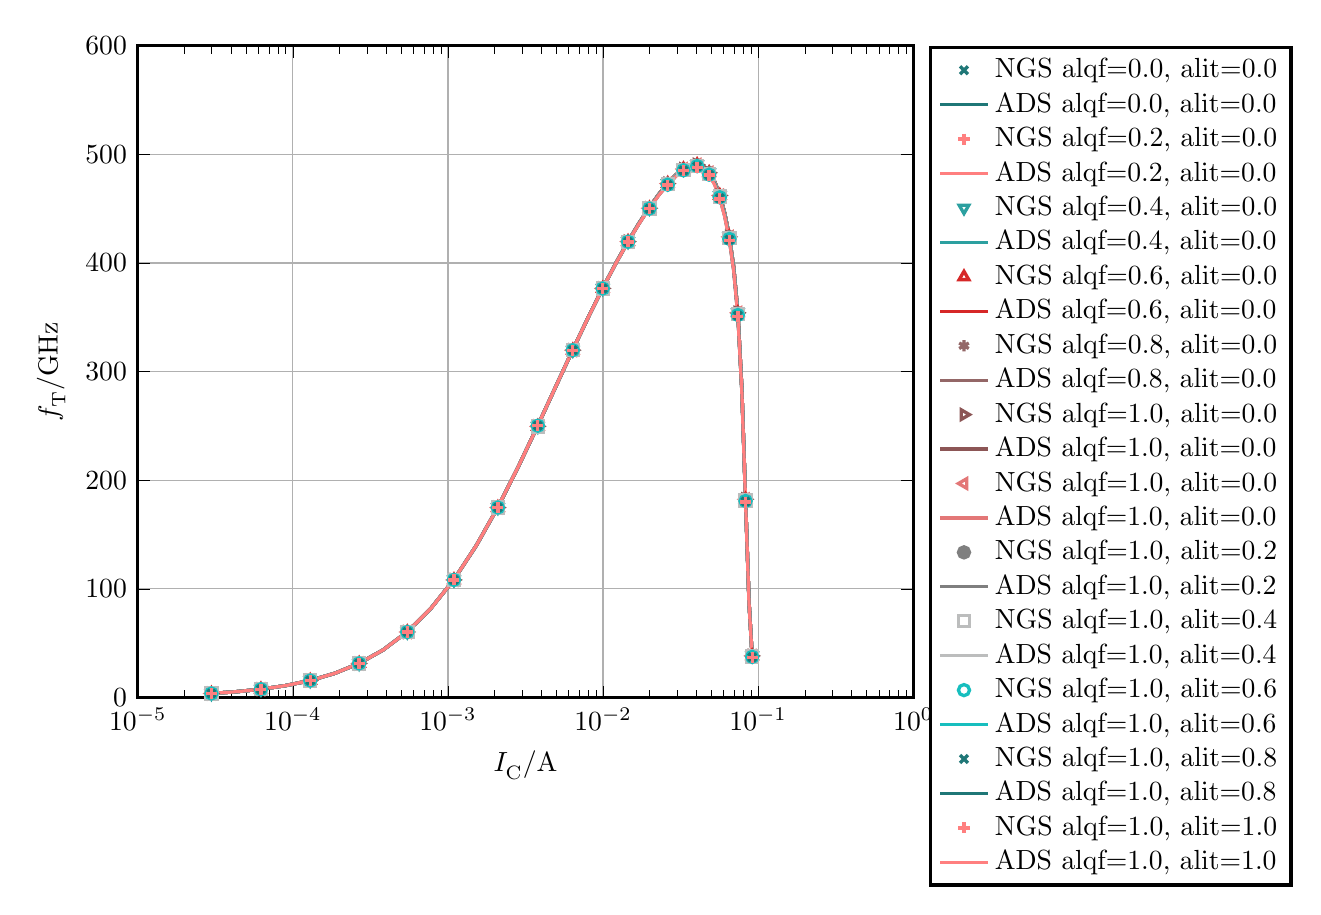
\begin{tikzpicture}[font=\normalsize]
\pgfplotsset{every axis/.append style={very thick}},
\definecolor{color0}{rgb}{0.12157, 0.46667, 0.46667}
\definecolor{color1}{rgb}{1.00000, 0.49804, 0.49804}
\definecolor{color2}{rgb}{0.17255, 0.62745, 0.62745}
\definecolor{color3}{rgb}{0.83922, 0.15294, 0.15294}
\definecolor{color4}{rgb}{0.58039, 0.40392, 0.40392}
\definecolor{color5}{rgb}{0.54902, 0.33725, 0.33725}
\definecolor{color6}{rgb}{0.89020, 0.46667, 0.46667}
\definecolor{color7}{rgb}{0.49804, 0.49804, 0.49804}
\definecolor{color8}{rgb}{0.73725, 0.74118, 0.74118}
\definecolor{color9}{rgb}{0.09020, 0.74510, 0.74510}

\begin{axis}[
width=4.5in,
xlabel={$I_{\mathrm{C}}^{}/\si{\ampere}$},
ylabel={$f_{\mathrm{T}}^{}/\si{\giga\hertz}$},
xmode=log,
xmin=1e-05,
xmax=1,
restrict x to domain=-5:0,
log basis x=10,
ymin=0,
ymax=600,
restrict y to domain=0:600,
log basis y=10,
xmajorgrids,
enlargelimits=false,
scaled ticks=false,
ymajorgrids,
x tick style={color=black},
y tick style={color=black},
x grid style={white!69.01960784313725!black},
y grid style={white!69.01960784313725!black},
/tikz/mark repeat=2,
legend style={at={(1.02,1.00)}, anchor=north west,legend cell align=left, align=left},
]
\addplot [color=color0, only marks, mark=x, mark options={solid}, mark phase=0, ]
  table[row sep=crcr, x expr=\thisrowno{0}*1.000000e+00, y expr=\thisrowno{1}*1.000000e-09]{
2.98396e-05 3.7103e+09\\
4.31177e-05 5.3303e+09\\
6.225e-05 7.65253e+09\\
8.97943e-05 1.09417e+10\\
0.000129401 1.56223e+10\\
0.000186243 2.21828e+10\\
0.000267564 3.13818e+10\\
0.000383354 4.38786e+10\\
0.000547084 6.03275e+10\\
0.000776382 8.18374e+10\\
0.00109339 1.08568e+11\\
0.00152451 1.40064e+11\\
0.00209913 1.74873e+11\\
0.00284735 2.1259e+11\\
0.00379703 2.50195e+11\\
0.00497087 2.8593e+11\\
0.00638447 3.19761e+11\\
0.00804567 3.49817e+11\\
0.0099552 3.76643e+11\\
0.012108 3.99286e+11\\
0.0144948 4.19769e+11\\
0.0171038 4.36956e+11\\
0.0199213 4.51143e+11\\
0.0229333 4.63334e+11\\
0.0261255 4.72548e+11\\
0.0294841 4.8106e+11\\
0.0329955 4.85948e+11\\
0.0366471 4.90655e+11\\
0.0404269 4.91097e+11\\
0.0443236 4.88864e+11\\
0.0483264 4.83167e+11\\
0.0524253 4.74985e+11\\
0.0566106 4.62728e+11\\
0.060873 4.45371e+11\\
0.0652035 4.24128e+11\\
0.0695925 3.96258e+11\\
0.0740296 3.54461e+11\\
0.0784992 2.84981e+11\\
0.08297 1.82551e+11\\
0.0873655 8.81619e+10\\
0.0915303 3.83321e+10\\
};
\addlegendentry{NGS alqf=0.0, alit=0.0}
\addplot [color=color0, solid,  mark phase=0, ]
  table[row sep=crcr, x expr=\thisrowno{0}*1.000000e+00, y expr=\thisrowno{1}*1.000000e-09]{
2.98384e-05 3.70997e+09\\
4.31161e-05 5.33215e+09\\
6.22476e-05 7.65375e+09\\
8.97908e-05 1.09652e+10\\
0.000129396 1.56617e+10\\
0.000186236 2.22643e+10\\
0.000267554 3.1429e+10\\
0.000383339 4.39242e+10\\
0.000547063 6.05531e+10\\
0.000776351 8.19942e+10\\
0.00109335 1.08568e+11\\
0.00152446 1.39988e+11\\
0.00209905 1.75236e+11\\
0.00284725 2.1267e+11\\
0.0037969 2.50381e+11\\
0.00497072 2.86632e+11\\
0.00638428 3.20174e+11\\
0.00804546 3.50328e+11\\
0.00995495 3.76898e+11\\
0.0121077 4.00002e+11\\
0.0144945 4.19916e+11\\
0.0171034 4.36961e+11\\
0.019921 4.51429e+11\\
0.0229329 4.63552e+11\\
0.0261251 4.73476e+11\\
0.0294836 4.81254e+11\\
0.032995 4.86848e+11\\
0.0366466 4.90127e+11\\
0.0404264 4.90879e+11\\
0.0443231 4.88826e+11\\
0.0483259 4.83647e+11\\
0.0524248 4.75012e+11\\
0.0566101 4.62595e+11\\
0.0608725 4.46031e+11\\
0.0652029 4.24618e+11\\
0.069592 3.96247e+11\\
0.074029 3.54454e+11\\
0.0784986 2.85095e+11\\
0.0829694 1.82583e+11\\
0.0873649 8.81736e+10\\
0.0915297 3.83405e+10\\
};
\addlegendentry{ADS alqf=0.0, alit=0.0}
\addplot [color=color1, only marks, mark=+, mark options={solid}, mark phase=0, ]
  table[row sep=crcr, x expr=\thisrowno{0}*1.000000e+00, y expr=\thisrowno{1}*1.000000e-09]{
2.98396e-05 3.69841e+09\\
4.31177e-05 5.3303e+09\\
6.225e-05 7.62815e+09\\
8.97943e-05 1.09417e+10\\
0.000129401 1.56223e+10\\
0.000186243 2.21828e+10\\
0.000267564 3.13818e+10\\
0.000383354 4.38786e+10\\
0.000547084 6.03275e+10\\
0.000776382 8.18374e+10\\
0.00109339 1.08264e+11\\
0.00152451 1.39689e+11\\
0.00209913 1.74873e+11\\
0.00284735 2.1208e+11\\
0.00379703 2.49632e+11\\
0.00497087 2.86535e+11\\
0.00638447 3.19761e+11\\
0.00804567 3.49817e+11\\
0.0099552 3.76643e+11\\
0.012108 3.99285e+11\\
0.0144948 4.19768e+11\\
0.0171038 4.36286e+11\\
0.0199213 4.50478e+11\\
0.0229333 4.63333e+11\\
0.0261255 4.73198e+11\\
0.0294841 4.80418e+11\\
0.0329955 4.86576e+11\\
0.0366471 4.89422e+11\\
0.0404269 4.90498e+11\\
0.0443236 4.88287e+11\\
0.0483264 4.83166e+11\\
0.0524253 4.74984e+11\\
0.0566106 4.62244e+11\\
0.060873 4.4581e+11\\
0.0652035 4.24126e+11\\
0.0695925 3.95917e+11\\
0.0740296 3.54191e+11\\
0.0784992 2.84978e+11\\
0.08297 1.82546e+11\\
0.0873655 8.81528e+10\\
0.0915303 3.8334e+10\\
};
\addlegendentry{NGS alqf=0.2, alit=0.0}
\addplot [color=color1, solid,  mark phase=0, ]
  table[row sep=crcr, x expr=\thisrowno{0}*1.000000e+00, y expr=\thisrowno{1}*1.000000e-09]{
2.98384e-05 3.70997e+09\\
4.31161e-05 5.33215e+09\\
6.22476e-05 7.65375e+09\\
8.97908e-05 1.09652e+10\\
0.000129396 1.56617e+10\\
0.000186236 2.22643e+10\\
0.000267554 3.1429e+10\\
0.000383339 4.39242e+10\\
0.000547063 6.05531e+10\\
0.000776351 8.19942e+10\\
0.00109335 1.08568e+11\\
0.00152446 1.39988e+11\\
0.00209905 1.75236e+11\\
0.00284725 2.1267e+11\\
0.0037969 2.50381e+11\\
0.00497072 2.86632e+11\\
0.00638428 3.20174e+11\\
0.00804546 3.50328e+11\\
0.00995495 3.76898e+11\\
0.0121077 4.00002e+11\\
0.0144945 4.19916e+11\\
0.0171034 4.36961e+11\\
0.019921 4.51429e+11\\
0.0229329 4.63552e+11\\
0.0261251 4.73476e+11\\
0.0294836 4.81254e+11\\
0.032995 4.86848e+11\\
0.0366466 4.90127e+11\\
0.0404264 4.90879e+11\\
0.0443231 4.88826e+11\\
0.0483259 4.83647e+11\\
0.0524248 4.75012e+11\\
0.0566101 4.62595e+11\\
0.0608725 4.46031e+11\\
0.0652029 4.24618e+11\\
0.069592 3.96246e+11\\
0.074029 3.54454e+11\\
0.0784986 2.85095e+11\\
0.0829694 1.82583e+11\\
0.0873649 8.81736e+10\\
0.0915297 3.83406e+10\\
};
\addlegendentry{ADS alqf=0.2, alit=0.0}
\addplot [color=color2, only marks, mark=triangle, mark options={solid, rotate=180}, mark phase=0, ]
  table[row sep=crcr, x expr=\thisrowno{0}*1.000000e+00, y expr=\thisrowno{1}*1.000000e-09]{
2.98396e-05 3.69841e+09\\
4.31177e-05 5.3303e+09\\
6.225e-05 7.62815e+09\\
8.97943e-05 1.09417e+10\\
0.000129401 1.56223e+10\\
0.000186243 2.21828e+10\\
0.000267564 3.13818e+10\\
0.000383354 4.38786e+10\\
0.000547084 6.03275e+10\\
0.000776382 8.18374e+10\\
0.00109339 1.08264e+11\\
0.00152451 1.39689e+11\\
0.00209913 1.74873e+11\\
0.00284735 2.1208e+11\\
0.00379703 2.49632e+11\\
0.00497087 2.86534e+11\\
0.00638447 3.1976e+11\\
0.00804567 3.49817e+11\\
0.0099552 3.76642e+11\\
0.012108 3.99285e+11\\
0.0144948 4.19768e+11\\
0.0171038 4.36285e+11\\
0.0199213 4.50478e+11\\
0.0229333 4.63332e+11\\
0.0261255 4.73197e+11\\
0.0294841 4.80417e+11\\
0.0329955 4.86575e+11\\
0.0366471 4.89421e+11\\
0.0404269 4.90497e+11\\
0.0443236 4.88286e+11\\
0.0483264 4.83164e+11\\
0.0524253 4.74982e+11\\
0.0566106 4.62243e+11\\
0.060873 4.45808e+11\\
0.0652035 4.24125e+11\\
0.0695925 3.95915e+11\\
0.0740296 3.54189e+11\\
0.0784992 2.84975e+11\\
0.08297 1.82541e+11\\
0.0873655 8.81431e+10\\
0.0915303 3.83361e+10\\
};
\addlegendentry{NGS alqf=0.4, alit=0.0}
\addplot [color=color2, solid,  mark phase=0, ]
  table[row sep=crcr, x expr=\thisrowno{0}*1.000000e+00, y expr=\thisrowno{1}*1.000000e-09]{
2.98384e-05 3.70997e+09\\
4.31161e-05 5.33215e+09\\
6.22476e-05 7.65375e+09\\
8.97908e-05 1.09652e+10\\
0.000129396 1.56617e+10\\
0.000186236 2.22643e+10\\
0.000267554 3.1429e+10\\
0.000383339 4.39242e+10\\
0.000547063 6.05531e+10\\
0.000776351 8.19942e+10\\
0.00109335 1.08568e+11\\
0.00152446 1.39988e+11\\
0.00209905 1.75236e+11\\
0.00284725 2.1267e+11\\
0.0037969 2.50381e+11\\
0.00497072 2.86632e+11\\
0.00638428 3.20174e+11\\
0.00804546 3.50328e+11\\
0.00995495 3.76898e+11\\
0.0121077 4.00002e+11\\
0.0144945 4.19916e+11\\
0.0171034 4.3696e+11\\
0.019921 4.51429e+11\\
0.0229329 4.63552e+11\\
0.0261251 4.73476e+11\\
0.0294836 4.81254e+11\\
0.032995 4.86848e+11\\
0.0366466 4.90127e+11\\
0.0404264 4.90879e+11\\
0.0443231 4.88826e+11\\
0.0483259 4.83647e+11\\
0.0524248 4.75012e+11\\
0.0566101 4.62595e+11\\
0.0608725 4.46031e+11\\
0.0652029 4.24618e+11\\
0.069592 3.96246e+11\\
0.074029 3.54454e+11\\
0.0784986 2.85095e+11\\
0.0829694 1.82583e+11\\
0.0873649 8.81741e+10\\
0.0915297 3.83421e+10\\
};
\addlegendentry{ADS alqf=0.4, alit=0.0}
\addplot [color=color3, only marks, mark=triangle, mark options={solid, rotate=0}, mark phase=0, ]
  table[row sep=crcr, x expr=\thisrowno{0}*1.000000e+00, y expr=\thisrowno{1}*1.000000e-09]{
2.98396e-05 3.69841e+09\\
4.31177e-05 5.3303e+09\\
6.225e-05 7.62815e+09\\
8.97943e-05 1.09417e+10\\
0.000129401 1.56223e+10\\
0.000186243 2.21828e+10\\
0.000267564 3.13818e+10\\
0.000383354 4.38786e+10\\
0.000547084 6.03275e+10\\
0.000776382 8.18374e+10\\
0.00109339 1.08264e+11\\
0.00152451 1.39689e+11\\
0.00209913 1.74873e+11\\
0.00284735 2.1208e+11\\
0.00379703 2.49632e+11\\
0.00497087 2.86534e+11\\
0.00638447 3.1976e+11\\
0.00804567 3.49816e+11\\
0.0099552 3.76642e+11\\
0.012108 3.99284e+11\\
0.0144948 4.19767e+11\\
0.0171038 4.36284e+11\\
0.0199213 4.50477e+11\\
0.0229333 4.63331e+11\\
0.0261255 4.73196e+11\\
0.0294841 4.80416e+11\\
0.0329955 4.86574e+11\\
0.0366471 4.8942e+11\\
0.0404269 4.90496e+11\\
0.0443236 4.88284e+11\\
0.0483264 4.83163e+11\\
0.0524253 4.74981e+11\\
0.0566106 4.62241e+11\\
0.060873 4.45807e+11\\
0.0652035 4.24123e+11\\
0.0695925 3.95913e+11\\
0.0740296 3.54186e+11\\
0.0784992 2.84973e+11\\
0.08297 1.82537e+11\\
0.0873655 8.81506e+10\\
0.0915303 3.83384e+10\\
};
\addlegendentry{NGS alqf=0.6, alit=0.0}
\addplot [color=color3, solid,  mark phase=0, ]
  table[row sep=crcr, x expr=\thisrowno{0}*1.000000e+00, y expr=\thisrowno{1}*1.000000e-09]{
2.98384e-05 3.70997e+09\\
4.31161e-05 5.33215e+09\\
6.22476e-05 7.65375e+09\\
8.97908e-05 1.09652e+10\\
0.000129396 1.56617e+10\\
0.000186236 2.22643e+10\\
0.000267554 3.1429e+10\\
0.000383339 4.39242e+10\\
0.000547063 6.05531e+10\\
0.000776351 8.19942e+10\\
0.00109335 1.08568e+11\\
0.00152446 1.39988e+11\\
0.00209905 1.75236e+11\\
0.00284725 2.1267e+11\\
0.0037969 2.50381e+11\\
0.00497072 2.86632e+11\\
0.00638428 3.20174e+11\\
0.00804546 3.50328e+11\\
0.00995495 3.76898e+11\\
0.0121077 4.00002e+11\\
0.0144945 4.19916e+11\\
0.0171034 4.3696e+11\\
0.019921 4.51429e+11\\
0.0229329 4.63552e+11\\
0.0261251 4.73476e+11\\
0.0294836 4.81254e+11\\
0.032995 4.86848e+11\\
0.0366466 4.90127e+11\\
0.0404264 4.90879e+11\\
0.0443231 4.88826e+11\\
0.0483259 4.83647e+11\\
0.0524248 4.75012e+11\\
0.0566101 4.62595e+11\\
0.0608725 4.46031e+11\\
0.0652029 4.24618e+11\\
0.069592 3.96247e+11\\
0.074029 3.54454e+11\\
0.0784986 2.85096e+11\\
0.0829694 1.82583e+11\\
0.0873649 8.81752e+10\\
0.0915297 3.83449e+10\\
};
\addlegendentry{ADS alqf=0.6, alit=0.0}
\addplot [color=color4, only marks, mark=asterisk, mark options={solid}, mark phase=0, ]
  table[row sep=crcr, x expr=\thisrowno{0}*1.000000e+00, y expr=\thisrowno{1}*1.000000e-09]{
2.98396e-05 3.69841e+09\\
4.31177e-05 5.3303e+09\\
6.225e-05 7.62815e+09\\
8.97943e-05 1.09417e+10\\
0.000129401 1.56223e+10\\
0.000186243 2.21828e+10\\
0.000267564 3.13818e+10\\
0.000383354 4.38786e+10\\
0.000547084 6.03275e+10\\
0.000776382 8.18373e+10\\
0.00109339 1.08264e+11\\
0.00152451 1.39689e+11\\
0.00209913 1.74873e+11\\
0.00284735 2.1208e+11\\
0.00379703 2.49632e+11\\
0.00497087 2.86534e+11\\
0.00638447 3.1976e+11\\
0.00804567 3.49816e+11\\
0.0099552 3.76641e+11\\
0.012108 3.99284e+11\\
0.0144948 4.19767e+11\\
0.0171038 4.36284e+11\\
0.0199213 4.50476e+11\\
0.0229333 4.63331e+11\\
0.0261255 4.73195e+11\\
0.0294841 4.80415e+11\\
0.0329955 4.86573e+11\\
0.0366471 4.89419e+11\\
0.0404269 4.90495e+11\\
0.0443236 4.88283e+11\\
0.0483264 4.83162e+11\\
0.0524253 4.7498e+11\\
0.0566106 4.6224e+11\\
0.060873 4.45805e+11\\
0.0652035 4.24121e+11\\
0.0695925 3.95912e+11\\
0.0740296 3.54184e+11\\
0.0784992 2.8497e+11\\
0.08297 1.82532e+11\\
0.0873655 8.81582e+10\\
0.0915303 3.83411e+10\\
};
\addlegendentry{NGS alqf=0.8, alit=0.0}
\addplot [color=color4, solid,  mark phase=0, ]
  table[row sep=crcr, x expr=\thisrowno{0}*1.000000e+00, y expr=\thisrowno{1}*1.000000e-09]{
2.98384e-05 3.70997e+09\\
4.31161e-05 5.33215e+09\\
6.22476e-05 7.65375e+09\\
8.97908e-05 1.09652e+10\\
0.000129396 1.56617e+10\\
0.000186236 2.22643e+10\\
0.000267554 3.1429e+10\\
0.000383339 4.39242e+10\\
0.000547063 6.05531e+10\\
0.000776351 8.19942e+10\\
0.00109335 1.08568e+11\\
0.00152446 1.39988e+11\\
0.00209905 1.75236e+11\\
0.00284725 2.1267e+11\\
0.0037969 2.50381e+11\\
0.00497072 2.86632e+11\\
0.00638428 3.20174e+11\\
0.00804546 3.50328e+11\\
0.00995495 3.76898e+11\\
0.0121077 4.00002e+11\\
0.0144945 4.19916e+11\\
0.0171034 4.36961e+11\\
0.019921 4.51429e+11\\
0.0229329 4.63552e+11\\
0.0261251 4.73476e+11\\
0.0294836 4.81254e+11\\
0.032995 4.86848e+11\\
0.0366466 4.90127e+11\\
0.0404264 4.90879e+11\\
0.0443231 4.88826e+11\\
0.0483259 4.83647e+11\\
0.0524248 4.75012e+11\\
0.0566101 4.62595e+11\\
0.0608725 4.46031e+11\\
0.0652029 4.24618e+11\\
0.069592 3.96247e+11\\
0.074029 3.54454e+11\\
0.0784986 2.85096e+11\\
0.0829694 1.82584e+11\\
0.0873649 8.81768e+10\\
0.0915297 3.83491e+10\\
};
\addlegendentry{ADS alqf=0.8, alit=0.0}
\addplot [color=color5, only marks, mark=triangle, mark options={solid, rotate=270}, mark phase=0, ]
  table[row sep=crcr, x expr=\thisrowno{0}*1.000000e+00, y expr=\thisrowno{1}*1.000000e-09]{
2.98396e-05 3.69841e+09\\
4.31177e-05 5.3303e+09\\
6.225e-05 7.62815e+09\\
8.97943e-05 1.09417e+10\\
0.000129401 1.56223e+10\\
0.000186243 2.21828e+10\\
0.000267564 3.13818e+10\\
0.000383354 4.38786e+10\\
0.000547084 6.03275e+10\\
0.000776382 8.18373e+10\\
0.00109339 1.08264e+11\\
0.00152451 1.39689e+11\\
0.00209913 1.74873e+11\\
0.00284735 2.1208e+11\\
0.00379703 2.49632e+11\\
0.00497087 2.86534e+11\\
0.00638447 3.1976e+11\\
0.00804567 3.49816e+11\\
0.0099552 3.76641e+11\\
0.012108 3.99283e+11\\
0.0144948 4.19766e+11\\
0.0171038 4.36283e+11\\
0.0199213 4.50476e+11\\
0.0229333 4.6333e+11\\
0.0261255 4.73194e+11\\
0.0294841 4.80414e+11\\
0.0329955 4.86572e+11\\
0.0366471 4.89418e+11\\
0.0404269 4.90494e+11\\
0.0443236 4.88282e+11\\
0.0483264 4.83161e+11\\
0.0524253 4.74978e+11\\
0.0566106 4.62239e+11\\
0.060873 4.45804e+11\\
0.0652035 4.2412e+11\\
0.0695925 3.9591e+11\\
0.0740296 3.54182e+11\\
0.0784992 2.84967e+11\\
0.08297 1.82527e+11\\
0.0873655 8.81659e+10\\
0.0915303 3.83475e+10\\
};
\addlegendentry{NGS alqf=1.0, alit=0.0}
\addplot [color=color5, solid,  mark phase=0, ]
  table[row sep=crcr, x expr=\thisrowno{0}*1.000000e+00, y expr=\thisrowno{1}*1.000000e-09]{
2.98384e-05 3.70997e+09\\
4.31161e-05 5.33215e+09\\
6.22476e-05 7.65375e+09\\
8.97908e-05 1.09652e+10\\
0.000129396 1.56617e+10\\
0.000186236 2.22643e+10\\
0.000267554 3.1429e+10\\
0.000383339 4.39242e+10\\
0.000547063 6.05531e+10\\
0.000776351 8.19942e+10\\
0.00109335 1.08568e+11\\
0.00152446 1.39988e+11\\
0.00209905 1.75236e+11\\
0.00284725 2.1267e+11\\
0.0037969 2.50381e+11\\
0.00497072 2.86632e+11\\
0.00638428 3.20174e+11\\
0.00804546 3.50328e+11\\
0.00995495 3.76898e+11\\
0.0121077 4.00002e+11\\
0.0144945 4.19916e+11\\
0.0171034 4.36961e+11\\
0.019921 4.51429e+11\\
0.0229329 4.63552e+11\\
0.0261251 4.73476e+11\\
0.0294836 4.81254e+11\\
0.032995 4.86848e+11\\
0.0366466 4.90127e+11\\
0.0404264 4.90879e+11\\
0.0443231 4.88826e+11\\
0.0483259 4.83648e+11\\
0.0524248 4.75012e+11\\
0.0566101 4.62595e+11\\
0.0608725 4.46031e+11\\
0.0652029 4.24618e+11\\
0.069592 3.96247e+11\\
0.074029 3.54454e+11\\
0.0784986 2.85096e+11\\
0.0829694 1.82585e+11\\
0.0873649 8.81791e+10\\
0.0915297 3.83546e+10\\
};
\addlegendentry{ADS alqf=1.0, alit=0.0}
\addplot [color=color6, only marks, mark=triangle, mark options={solid, rotate=90}, mark phase=0, ]
  table[row sep=crcr, x expr=\thisrowno{0}*1.000000e+00, y expr=\thisrowno{1}*1.000000e-09]{
2.98396e-05 3.69841e+09\\
4.31177e-05 5.3303e+09\\
6.225e-05 7.62815e+09\\
8.97943e-05 1.09417e+10\\
0.000129401 1.56223e+10\\
0.000186243 2.21828e+10\\
0.000267564 3.13818e+10\\
0.000383354 4.38786e+10\\
0.000547084 6.03275e+10\\
0.000776382 8.18373e+10\\
0.00109339 1.08264e+11\\
0.00152451 1.39689e+11\\
0.00209913 1.74873e+11\\
0.00284735 2.1208e+11\\
0.00379703 2.49632e+11\\
0.00497087 2.86534e+11\\
0.00638447 3.1976e+11\\
0.00804567 3.49816e+11\\
0.0099552 3.76641e+11\\
0.012108 3.99283e+11\\
0.0144948 4.19766e+11\\
0.0171038 4.36283e+11\\
0.0199213 4.50476e+11\\
0.0229333 4.6333e+11\\
0.0261255 4.73194e+11\\
0.0294841 4.80414e+11\\
0.0329955 4.86572e+11\\
0.0366471 4.89418e+11\\
0.0404269 4.90494e+11\\
0.0443236 4.88282e+11\\
0.0483264 4.83161e+11\\
0.0524253 4.74978e+11\\
0.0566106 4.62239e+11\\
0.060873 4.45804e+11\\
0.0652035 4.2412e+11\\
0.0695925 3.9591e+11\\
0.0740296 3.54182e+11\\
0.0784992 2.84967e+11\\
0.08297 1.82527e+11\\
0.0873655 8.81659e+10\\
0.0915303 3.83475e+10\\
};
\addlegendentry{NGS alqf=1.0, alit=0.0}
\addplot [color=color6, solid,  mark phase=0, ]
  table[row sep=crcr, x expr=\thisrowno{0}*1.000000e+00, y expr=\thisrowno{1}*1.000000e-09]{
2.98384e-05 3.70997e+09\\
4.31161e-05 5.33215e+09\\
6.22476e-05 7.65375e+09\\
8.97908e-05 1.09652e+10\\
0.000129396 1.56617e+10\\
0.000186236 2.22643e+10\\
0.000267554 3.1429e+10\\
0.000383339 4.39242e+10\\
0.000547063 6.05531e+10\\
0.000776351 8.19942e+10\\
0.00109335 1.08568e+11\\
0.00152446 1.39988e+11\\
0.00209905 1.75236e+11\\
0.00284725 2.1267e+11\\
0.0037969 2.50381e+11\\
0.00497072 2.86632e+11\\
0.00638428 3.20174e+11\\
0.00804546 3.50328e+11\\
0.00995495 3.76898e+11\\
0.0121077 4.00002e+11\\
0.0144945 4.19916e+11\\
0.0171034 4.36961e+11\\
0.019921 4.51429e+11\\
0.0229329 4.63552e+11\\
0.0261251 4.73476e+11\\
0.0294836 4.81254e+11\\
0.032995 4.86848e+11\\
0.0366466 4.90127e+11\\
0.0404264 4.90879e+11\\
0.0443231 4.88826e+11\\
0.0483259 4.83648e+11\\
0.0524248 4.75012e+11\\
0.0566101 4.62595e+11\\
0.0608725 4.46031e+11\\
0.0652029 4.24618e+11\\
0.069592 3.96247e+11\\
0.074029 3.54454e+11\\
0.0784986 2.85096e+11\\
0.0829694 1.82585e+11\\
0.0873649 8.81791e+10\\
0.0915297 3.83546e+10\\
};
\addlegendentry{ADS alqf=1.0, alit=0.0}
\addplot [color=color7, only marks, mark=*, mark options={solid, fill}, mark phase=0, ]
  table[row sep=crcr, x expr=\thisrowno{0}*1.000000e+00, y expr=\thisrowno{1}*1.000000e-09]{
2.98396e-05 3.69846e+09\\
4.31177e-05 5.33037e+09\\
6.225e-05 7.62826e+09\\
8.97943e-05 1.09419e+10\\
0.000129401 1.56226e+10\\
0.000186243 2.21834e+10\\
0.000267564 3.13828e+10\\
0.000383354 4.38804e+10\\
0.000547084 6.03306e+10\\
0.000776382 8.18423e+10\\
0.00109339 1.08272e+11\\
0.00152451 1.39699e+11\\
0.00209913 1.74887e+11\\
0.00284735 2.12095e+11\\
0.00379703 2.49646e+11\\
0.00497087 2.86543e+11\\
0.00638447 3.1976e+11\\
0.00804567 3.49802e+11\\
0.0099552 3.76611e+11\\
0.012108 3.99235e+11\\
0.0144948 4.19697e+11\\
0.0171038 4.36193e+11\\
0.0199213 4.50364e+11\\
0.0229333 4.63198e+11\\
0.0261255 4.73044e+11\\
0.0294841 4.80246e+11\\
0.0329955 4.85759e+11\\
0.0366471 4.8922e+11\\
0.0404269 4.89686e+11\\
0.0443236 4.88059e+11\\
0.0483264 4.82929e+11\\
0.0524253 4.7422e+11\\
0.0566106 4.61512e+11\\
0.060873 4.45115e+11\\
0.0652035 4.23871e+11\\
0.0695925 3.95326e+11\\
0.0740296 3.53677e+11\\
0.0784992 2.84406e+11\\
0.08297 1.81994e+11\\
0.0873655 8.77714e+10\\
0.0915303 3.80377e+10\\
};
\addlegendentry{NGS alqf=1.0, alit=0.2}
\addplot [color=color7, solid,  mark phase=0, ]
  table[row sep=crcr, x expr=\thisrowno{0}*1.000000e+00, y expr=\thisrowno{1}*1.000000e-09]{
2.98384e-05 3.71002e+09\\
4.31161e-05 5.33222e+09\\
6.22476e-05 7.65386e+09\\
8.97908e-05 1.09654e+10\\
0.000129396 1.5662e+10\\
0.000186236 2.22649e+10\\
0.000267554 3.143e+10\\
0.000383339 4.39261e+10\\
0.000547063 6.05563e+10\\
0.000776351 8.19996e+10\\
0.00109335 1.08576e+11\\
0.00152446 1.40001e+11\\
0.00209905 1.75253e+11\\
0.00284725 2.12691e+11\\
0.0037969 2.50403e+11\\
0.00497072 2.86652e+11\\
0.00638428 3.20187e+11\\
0.00804546 3.50328e+11\\
0.00995495 3.76879e+11\\
0.0121077 3.99959e+11\\
0.0144945 4.19842e+11\\
0.0171034 4.36852e+11\\
0.019921 4.51281e+11\\
0.0229329 4.63361e+11\\
0.0261251 4.7324e+11\\
0.0294836 4.80971e+11\\
0.032995 4.86515e+11\\
0.0366466 4.89744e+11\\
0.0404264 4.90445e+11\\
0.0443231 4.88342e+11\\
0.0483259 4.83116e+11\\
0.0524248 4.74436e+11\\
0.0566101 4.61978e+11\\
0.0608725 4.45378e+11\\
0.0652029 4.23937e+11\\
0.069592 3.9555e+11\\
0.074029 3.53763e+11\\
0.0784986 2.84455e+11\\
0.0829694 1.82061e+11\\
0.0873649 8.77896e+10\\
0.0915297 3.80449e+10\\
};
\addlegendentry{ADS alqf=1.0, alit=0.2}
\addplot [color=color8, only marks, mark=square, mark options={solid}, mark phase=0, ]
  table[row sep=crcr, x expr=\thisrowno{0}*1.000000e+00, y expr=\thisrowno{1}*1.000000e-09]{
2.98396e-05 3.69851e+09\\
4.31177e-05 5.33044e+09\\
6.225e-05 7.62837e+09\\
8.97943e-05 1.09421e+10\\
0.000129401 1.56229e+10\\
0.000186243 2.2184e+10\\
0.000267564 3.13838e+10\\
0.000383354 4.38822e+10\\
0.000547084 6.03336e+10\\
0.000776382 8.18474e+10\\
0.00109339 1.08279e+11\\
0.00152451 1.3971e+11\\
0.00209913 1.749e+11\\
0.00284735 2.12111e+11\\
0.00379703 2.4966e+11\\
0.00497087 2.86552e+11\\
0.00638447 3.1976e+11\\
0.00804567 3.49789e+11\\
0.0099552 3.76581e+11\\
0.012108 3.99186e+11\\
0.0144948 4.19627e+11\\
0.0171038 4.36102e+11\\
0.0199213 4.50253e+11\\
0.0229333 4.63067e+11\\
0.0261255 4.72893e+11\\
0.0294841 4.80078e+11\\
0.0329955 4.85575e+11\\
0.0366471 4.89021e+11\\
0.0404269 4.89474e+11\\
0.0443236 4.87837e+11\\
0.0483264 4.82149e+11\\
0.0524253 4.73465e+11\\
0.0566106 4.61268e+11\\
0.060873 4.44429e+11\\
0.0652035 4.22839e+11\\
0.0695925 3.94407e+11\\
0.0740296 3.52907e+11\\
0.0784992 2.83676e+11\\
0.08297 1.81465e+11\\
0.0873655 8.73806e+10\\
0.0915303 3.77333e+10\\
};
\addlegendentry{NGS alqf=1.0, alit=0.4}
\addplot [color=color8, solid,  mark phase=0, ]
  table[row sep=crcr, x expr=\thisrowno{0}*1.000000e+00, y expr=\thisrowno{1}*1.000000e-09]{
2.98384e-05 3.71008e+09\\
4.31161e-05 5.3323e+09\\
6.22476e-05 7.65397e+09\\
8.97908e-05 1.09655e+10\\
0.000129396 1.56623e+10\\
0.000186236 2.22655e+10\\
0.000267554 3.1431e+10\\
0.000383339 4.3928e+10\\
0.000547063 6.05595e+10\\
0.000776351 8.2005e+10\\
0.00109335 1.08585e+11\\
0.00152446 1.40013e+11\\
0.00209905 1.7527e+11\\
0.00284725 2.12711e+11\\
0.0037969 2.50425e+11\\
0.00497072 2.86672e+11\\
0.00638428 3.20199e+11\\
0.00804546 3.50328e+11\\
0.00995495 3.7686e+11\\
0.0121077 3.99915e+11\\
0.0144945 4.19768e+11\\
0.0171034 4.36743e+11\\
0.019921 4.51133e+11\\
0.0229329 4.63171e+11\\
0.0261251 4.73004e+11\\
0.0294836 4.80687e+11\\
0.032995 4.86182e+11\\
0.0366466 4.89361e+11\\
0.0404264 4.90012e+11\\
0.0443231 4.8786e+11\\
0.0483259 4.82586e+11\\
0.0524248 4.73861e+11\\
0.0566101 4.61362e+11\\
0.0608725 4.44727e+11\\
0.0652029 4.23258e+11\\
0.069592 3.94855e+11\\
0.074029 3.53073e+11\\
0.0784986 2.83817e+11\\
0.0829694 1.81541e+11\\
0.0873649 8.74038e+10\\
0.0915297 3.77405e+10\\
};
\addlegendentry{ADS alqf=1.0, alit=0.4}
\addplot [color=color9, only marks, mark=o, mark options={solid, fill}, mark phase=0, ]
  table[row sep=crcr, x expr=\thisrowno{0}*1.000000e+00, y expr=\thisrowno{1}*1.000000e-09]{
2.98396e-05 3.69857e+09\\
4.31177e-05 5.33052e+09\\
6.225e-05 7.62848e+09\\
8.97943e-05 1.09422e+10\\
0.000129401 1.56233e+10\\
0.000186243 2.21845e+10\\
0.000267564 3.13848e+10\\
0.000383354 4.3884e+10\\
0.000547084 6.03367e+10\\
0.000776382 8.18524e+10\\
0.00109339 1.08287e+11\\
0.00152451 1.39721e+11\\
0.00209913 1.74914e+11\\
0.00284735 2.12126e+11\\
0.00379703 2.50237e+11\\
0.00497087 2.86562e+11\\
0.00638447 3.1976e+11\\
0.00804567 3.49776e+11\\
0.0099552 3.76551e+11\\
0.012108 3.99137e+11\\
0.0144948 4.19558e+11\\
0.0171038 4.36012e+11\\
0.0199213 4.50142e+11\\
0.0229333 4.62935e+11\\
0.0261255 4.72094e+11\\
0.0294841 4.79911e+11\\
0.0329955 4.85391e+11\\
0.0366471 4.88211e+11\\
0.0404269 4.89263e+11\\
0.0443236 4.87041e+11\\
0.0483264 4.81372e+11\\
0.0524253 4.72711e+11\\
0.0566106 4.60545e+11\\
0.060873 4.43745e+11\\
0.0652035 4.22202e+11\\
0.0695925 3.94163e+11\\
0.0740296 3.52139e+11\\
0.0784992 2.8312e+11\\
0.08297 1.80938e+11\\
0.0873655 8.70102e+10\\
0.0915303 3.74343e+10\\
};
\addlegendentry{NGS alqf=1.0, alit=0.6}
\addplot [color=color9, solid,  mark phase=0, ]
  table[row sep=crcr, x expr=\thisrowno{0}*1.000000e+00, y expr=\thisrowno{1}*1.000000e-09]{
2.98384e-05 3.71013e+09\\
4.31161e-05 5.33237e+09\\
6.22476e-05 7.65408e+09\\
8.97908e-05 1.09657e+10\\
0.000129396 1.56626e+10\\
0.000186236 2.2266e+10\\
0.000267554 3.14321e+10\\
0.000383339 4.39298e+10\\
0.000547063 6.05628e+10\\
0.000776351 8.20104e+10\\
0.00109335 1.08593e+11\\
0.00152446 1.40026e+11\\
0.00209905 1.75287e+11\\
0.00284725 2.12732e+11\\
0.0037969 2.50447e+11\\
0.00497072 2.86692e+11\\
0.00638428 3.20212e+11\\
0.00804546 3.50328e+11\\
0.00995495 3.76841e+11\\
0.0121077 3.99871e+11\\
0.0144945 4.19694e+11\\
0.0171034 4.36634e+11\\
0.019921 4.50985e+11\\
0.0229329 4.6298e+11\\
0.0261251 4.72768e+11\\
0.0294836 4.80404e+11\\
0.032995 4.8585e+11\\
0.0366466 4.88979e+11\\
0.0404264 4.8958e+11\\
0.0443231 4.87378e+11\\
0.0483259 4.82057e+11\\
0.0524248 4.73287e+11\\
0.0566101 4.60747e+11\\
0.0608725 4.44077e+11\\
0.0652029 4.22582e+11\\
0.069592 3.94163e+11\\
0.074029 3.52387e+11\\
0.0784986 2.83182e+11\\
0.0829694 1.81024e+11\\
0.0873649 8.70215e+10\\
0.0915297 3.74413e+10\\
};
\addlegendentry{ADS alqf=1.0, alit=0.6}
\addplot [color=color0, only marks, mark=x, mark options={solid}, mark phase=0, ]
  table[row sep=crcr, x expr=\thisrowno{0}*1.000000e+00, y expr=\thisrowno{1}*1.000000e-09]{
2.98396e-05 3.69862e+09\\
4.31177e-05 5.33059e+09\\
6.225e-05 7.62859e+09\\
8.97943e-05 1.09424e+10\\
0.000129401 1.56236e+10\\
0.000186243 2.21851e+10\\
0.000267564 3.13858e+10\\
0.000383354 4.38858e+10\\
0.000547084 6.03398e+10\\
0.000776382 8.18574e+10\\
0.00109339 1.08295e+11\\
0.00152451 1.39732e+11\\
0.00209913 1.74928e+11\\
0.00284735 2.12141e+11\\
0.00379703 2.50251e+11\\
0.00497087 2.86571e+11\\
0.00638447 3.1976e+11\\
0.00804567 3.49763e+11\\
0.0099552 3.76522e+11\\
0.012108 3.99088e+11\\
0.0144948 4.19488e+11\\
0.0171038 4.35922e+11\\
0.0199213 4.50032e+11\\
0.0229333 4.62147e+11\\
0.0261255 4.71944e+11\\
0.0294841 4.79743e+11\\
0.0329955 4.85208e+11\\
0.0366471 4.88013e+11\\
0.0404269 4.89053e+11\\
0.0443236 4.86248e+11\\
0.0483264 4.81141e+11\\
0.0524253 4.72473e+11\\
0.0566106 4.59824e+11\\
0.060873 4.43063e+11\\
0.0652035 4.21567e+11\\
0.0695925 3.9325e+11\\
0.0740296 3.5164e+11\\
0.0784992 2.82396e+11\\
0.08297 1.80485e+11\\
0.0873655 8.66265e+10\\
0.0915303 3.71403e+10\\
};
\addlegendentry{NGS alqf=1.0, alit=0.8}
\addplot [color=color0, solid,  mark phase=0, ]
  table[row sep=crcr, x expr=\thisrowno{0}*1.000000e+00, y expr=\thisrowno{1}*1.000000e-09]{
2.98384e-05 3.71018e+09\\
4.31161e-05 5.33244e+09\\
6.22476e-05 7.6542e+09\\
8.97908e-05 1.09659e+10\\
0.000129396 1.56629e+10\\
0.000186236 2.22666e+10\\
0.000267554 3.14331e+10\\
0.000383339 4.39317e+10\\
0.000547063 6.0566e+10\\
0.000776351 8.20158e+10\\
0.00109335 1.08602e+11\\
0.00152446 1.40038e+11\\
0.00209905 1.75304e+11\\
0.00284725 2.12752e+11\\
0.0037969 2.50469e+11\\
0.00497072 2.86712e+11\\
0.00638428 3.20225e+11\\
0.00804546 3.50328e+11\\
0.00995495 3.76822e+11\\
0.0121077 3.99827e+11\\
0.0144945 4.1962e+11\\
0.0171034 4.36525e+11\\
0.019921 4.50837e+11\\
0.0229329 4.6279e+11\\
0.0261251 4.72532e+11\\
0.0294836 4.80121e+11\\
0.032995 4.85518e+11\\
0.0366466 4.88597e+11\\
0.0404264 4.89149e+11\\
0.0443231 4.86898e+11\\
0.0483259 4.81529e+11\\
0.0524248 4.72714e+11\\
0.0566101 4.60135e+11\\
0.0608725 4.4343e+11\\
0.0652029 4.21908e+11\\
0.069592 3.93473e+11\\
0.074029 3.51703e+11\\
0.0784986 2.82549e+11\\
0.0829694 1.80509e+11\\
0.0873649 8.66427e+10\\
0.0915297 3.71472e+10\\
};
\addlegendentry{ADS alqf=1.0, alit=0.8}
\addplot [color=color1, only marks, mark=+, mark options={solid}, mark phase=0, ]
  table[row sep=crcr, x expr=\thisrowno{0}*1.000000e+00, y expr=\thisrowno{1}*1.000000e-09]{
2.98396e-05 3.69867e+09\\
4.31177e-05 5.33066e+09\\
6.225e-05 7.6287e+09\\
8.97943e-05 1.09426e+10\\
0.000129401 1.56239e+10\\
0.000186243 2.21857e+10\\
0.000267564 3.13869e+10\\
0.000383354 4.38876e+10\\
0.000547084 6.03428e+10\\
0.000776382 8.18625e+10\\
0.00109339 1.08303e+11\\
0.00152451 1.39743e+11\\
0.00209913 1.74942e+11\\
0.00284735 2.12157e+11\\
0.00379703 2.50266e+11\\
0.00497087 2.86581e+11\\
0.00638447 3.1976e+11\\
0.00804567 3.4975e+11\\
0.0099552 3.76492e+11\\
0.012108 3.99039e+11\\
0.0144948 4.19419e+11\\
0.0171038 4.35832e+11\\
0.0199213 4.49921e+11\\
0.0229333 4.62016e+11\\
0.0261255 4.71794e+11\\
0.0294841 4.79576e+11\\
0.0329955 4.85025e+11\\
0.0366471 4.87815e+11\\
0.0404269 4.88249e+11\\
0.0443236 4.86027e+11\\
0.0483264 4.80911e+11\\
0.0524253 4.71723e+11\\
0.0566106 4.59105e+11\\
0.060873 4.42383e+11\\
0.0652035 4.20934e+11\\
0.0695925 3.92674e+11\\
0.0740296 3.50615e+11\\
0.0784992 2.81845e+11\\
0.08297 1.79895e+11\\
0.0873655 8.62464e+10\\
0.0915303 3.68515e+10\\
};
\addlegendentry{NGS alqf=1.0, alit=1.0}
\addplot [color=color1, solid,  mark phase=0, ]
  table[row sep=crcr, x expr=\thisrowno{0}*1.000000e+00, y expr=\thisrowno{1}*1.000000e-09]{
2.98384e-05 3.71024e+09\\
4.31161e-05 5.33252e+09\\
6.22476e-05 7.65431e+09\\
8.97908e-05 1.09661e+10\\
0.000129396 1.56633e+10\\
0.000186236 2.22672e+10\\
0.000267554 3.14342e+10\\
0.000383339 4.39336e+10\\
0.000547063 6.05693e+10\\
0.000776351 8.20212e+10\\
0.00109335 1.0861e+11\\
0.00152446 1.40051e+11\\
0.00209905 1.75321e+11\\
0.00284725 2.12773e+11\\
0.0037969 2.50491e+11\\
0.00497072 2.86732e+11\\
0.00638428 3.20238e+11\\
0.00804546 3.50327e+11\\
0.00995495 3.76803e+11\\
0.0121077 3.99783e+11\\
0.0144945 4.19547e+11\\
0.0171034 4.36416e+11\\
0.019921 4.5069e+11\\
0.0229329 4.626e+11\\
0.0261251 4.72297e+11\\
0.0294836 4.79838e+11\\
0.032995 4.85187e+11\\
0.0366466 4.88216e+11\\
0.0404264 4.88718e+11\\
0.0443231 4.86418e+11\\
0.0483259 4.81002e+11\\
0.0524248 4.72143e+11\\
0.0566101 4.59524e+11\\
0.0608725 4.42785e+11\\
0.0652029 4.21236e+11\\
0.069592 3.92786e+11\\
0.074029 3.51022e+11\\
0.0784986 2.8192e+11\\
0.0829694 1.79998e+11\\
0.0873649 8.62673e+10\\
0.0915297 3.68581e+10\\
};
\addlegendentry{ADS alqf=1.0, alit=1.0}
\end{axis}

\end{tikzpicture}
%
\caption{FT(VBE)}%
\label{FT(VBE)}%
\end{figure}

%


\begin{figure}[h!]%
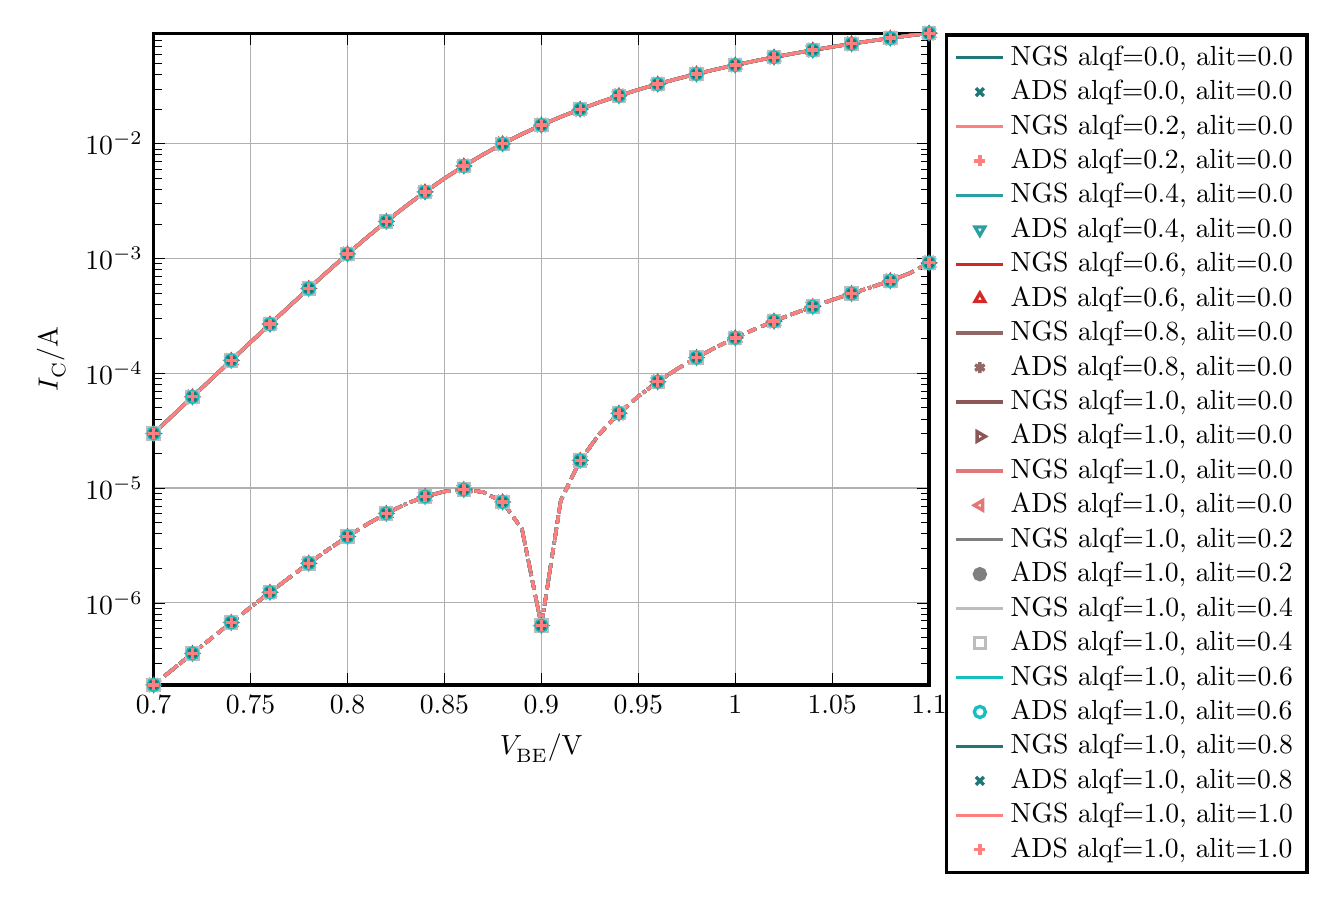
\begin{tikzpicture}[font=\normalsize]
\pgfplotsset{every axis/.append style={very thick}},
\definecolor{color0}{rgb}{0.12157, 0.46667, 0.46667}
\definecolor{color1}{rgb}{1.00000, 0.49804, 0.49804}
\definecolor{color2}{rgb}{0.17255, 0.62745, 0.62745}
\definecolor{color3}{rgb}{0.83922, 0.15294, 0.15294}
\definecolor{color4}{rgb}{0.58039, 0.40392, 0.40392}
\definecolor{color5}{rgb}{0.54902, 0.33725, 0.33725}
\definecolor{color6}{rgb}{0.89020, 0.46667, 0.46667}
\definecolor{color7}{rgb}{0.49804, 0.49804, 0.49804}
\definecolor{color8}{rgb}{0.73725, 0.74118, 0.74118}
\definecolor{color9}{rgb}{0.09020, 0.74510, 0.74510}

\begin{axis}[
width=4.5in,
xlabel={$V_{\mathrm{BE}}^{}/\si{\volt}$},
ylabel={$I_{\mathrm{C}}^{}/\si{\ampere}$},
ymode=log,
% xmin=0,
% xmax=0,
% restrict x to domain=0:1,
log basis x=10,
% ymin=0,
% ymax=0,
% restrict y to domain=0:1,
log basis y=10,
xmajorgrids,
enlargelimits=false,
scaled ticks=false,
ymajorgrids,
x tick style={color=black},
y tick style={color=black},
x grid style={white!69.01960784313725!black},
y grid style={white!69.01960784313725!black},
/tikz/mark repeat=2,
legend style={at={(1.02,1.00)}, anchor=north west,legend cell align=left, align=left},
]
\addplot [color=color0, solid,  mark phase=0, ]
  table[row sep=crcr, x expr=\thisrowno{0}*1.000000e+00, y expr=\thisrowno{1}*1.000000e+00]{
0.7 2.98396e-05\\
0.71 4.31177e-05\\
0.72 6.225e-05\\
0.73 8.97943e-05\\
0.74 0.000129401\\
0.75 0.000186243\\
0.76 0.000267564\\
0.77 0.000383354\\
0.78 0.000547084\\
0.79 0.000776382\\
0.8 0.00109339\\
0.81 0.00152451\\
0.82 0.00209913\\
0.83 0.00284735\\
0.84 0.00379703\\
0.85 0.00497087\\
0.86 0.00638447\\
0.87 0.00804567\\
0.88 0.0099552\\
0.89 0.012108\\
0.9 0.0144948\\
0.91 0.0171038\\
0.92 0.0199213\\
0.93 0.0229333\\
0.94 0.0261255\\
0.95 0.0294841\\
0.96 0.0329955\\
0.97 0.0366471\\
0.98 0.0404269\\
0.99 0.0443236\\
1 0.0483264\\
1.01 0.0524253\\
1.02 0.0566106\\
1.03 0.060873\\
1.04 0.0652035\\
1.05 0.0695925\\
1.06 0.0740296\\
1.07 0.0784992\\
1.08 0.08297\\
1.09 0.0873655\\
1.1 0.0915303\\
};
\addlegendentry{NGS alqf=0.0, alit=0.0}
\addplot [color=color0, only marks, mark=x, mark options={solid}, mark phase=0, ]
  table[row sep=crcr, x expr=\thisrowno{0}*1.000000e+00, y expr=\thisrowno{1}*1.000000e+00]{
0.7 2.98384e-05\\
0.71 4.31161e-05\\
0.72 6.22476e-05\\
0.73 8.97908e-05\\
0.74 0.000129396\\
0.75 0.000186236\\
0.76 0.000267554\\
0.77 0.000383339\\
0.78 0.000547063\\
0.79 0.000776351\\
0.8 0.00109335\\
0.81 0.00152446\\
0.82 0.00209905\\
0.83 0.00284725\\
0.84 0.0037969\\
0.85 0.00497072\\
0.86 0.00638428\\
0.87 0.00804546\\
0.88 0.00995495\\
0.89 0.0121077\\
0.9 0.0144945\\
0.91 0.0171034\\
0.92 0.019921\\
0.93 0.0229329\\
0.94 0.0261251\\
0.95 0.0294836\\
0.96 0.032995\\
0.97 0.0366466\\
0.98 0.0404264\\
0.99 0.0443231\\
1 0.0483259\\
1.01 0.0524248\\
1.02 0.0566101\\
1.03 0.0608725\\
1.04 0.0652029\\
1.05 0.069592\\
1.06 0.074029\\
1.07 0.0784986\\
1.08 0.0829694\\
1.09 0.0873649\\
1.1 0.0915297\\
};
\addlegendentry{ADS alqf=0.0, alit=0.0}
\addplot [color=color0, dashed,  mark phase=0, forget plot, ]
  table[row sep=crcr, x expr=\thisrowno{0}*1.000000e+00, y expr=\thisrowno{1}*1.000000e+00]{
0.7 1.92566e-07\\
0.71 2.64497e-07\\
0.72 3.62279e-07\\
0.73 4.94792e-07\\
0.74 6.737e-07\\
0.75 9.14018e-07\\
0.76 1.23452e-06\\
0.77 1.65766e-06\\
0.78 2.20837e-06\\
0.79 2.91096e-06\\
0.8 3.78297e-06\\
0.81 4.82508e-06\\
0.82 6.00723e-06\\
0.83 7.25302e-06\\
0.84 8.42655e-06\\
0.85 9.32676e-06\\
0.86 9.69201e-06\\
0.87 9.21432e-06\\
0.88 7.55919e-06\\
0.89 4.38615e-06\\
0.9 6.33686e-07\\
0.91 7.80474e-06\\
0.92 1.73992e-05\\
0.93 2.96533e-05\\
0.94 4.47678e-05\\
0.95 6.29099e-05\\
0.96 8.42176e-05\\
0.97 0.000108805\\
0.98 0.000136769\\
0.99 0.000168195\\
1 0.000203163\\
1.01 0.000241758\\
1.02 0.000284075\\
1.03 0.000330235\\
1.04 0.000380401\\
1.05 0.000434847\\
1.06 0.000494152\\
1.07 0.000559961\\
1.08 0.00063757\\
1.09 0.000743217\\
1.1 0.000914907\\
};
% \addlegendentry{}
\addplot [color=color0, dashdotted, mark=x, mark options={solid}, mark phase=0, forget plot, ]
  table[row sep=crcr, x expr=\thisrowno{0}*1.000000e+00, y expr=\thisrowno{1}*1.000000e+00]{
0.7 1.92559e-07\\
0.71 2.64488e-07\\
0.72 3.62265e-07\\
0.73 4.94774e-07\\
0.74 6.73673e-07\\
0.75 9.13982e-07\\
0.76 1.23448e-06\\
0.77 1.6576e-06\\
0.78 2.20828e-06\\
0.79 2.91085e-06\\
0.8 3.78283e-06\\
0.81 4.82491e-06\\
0.82 6.00703e-06\\
0.83 7.25279e-06\\
0.84 8.42632e-06\\
0.85 9.32655e-06\\
0.86 9.69185e-06\\
0.87 9.21425e-06\\
0.88 7.55926e-06\\
0.89 4.38638e-06\\
0.9 6.33234e-07\\
0.91 7.80403e-06\\
0.92 1.73982e-05\\
0.93 2.9652e-05\\
0.94 4.47661e-05\\
0.95 6.29078e-05\\
0.96 8.42152e-05\\
0.97 0.000108802\\
0.98 0.000136766\\
0.99 0.000168191\\
1 0.000203159\\
1.01 0.000241753\\
1.02 0.00028407\\
1.03 0.000330229\\
1.04 0.000380395\\
1.05 0.00043484\\
1.06 0.000494145\\
1.07 0.000559952\\
1.08 0.000637559\\
1.09 0.0007432\\
1.1 0.000914878\\
};
% \addlegendentry{}
\addplot [color=color1, solid,  mark phase=0, ]
  table[row sep=crcr, x expr=\thisrowno{0}*1.000000e+00, y expr=\thisrowno{1}*1.000000e+00]{
0.7 2.98396e-05\\
0.71 4.31177e-05\\
0.72 6.225e-05\\
0.73 8.97943e-05\\
0.74 0.000129401\\
0.75 0.000186243\\
0.76 0.000267564\\
0.77 0.000383354\\
0.78 0.000547084\\
0.79 0.000776382\\
0.8 0.00109339\\
0.81 0.00152451\\
0.82 0.00209913\\
0.83 0.00284735\\
0.84 0.00379703\\
0.85 0.00497087\\
0.86 0.00638447\\
0.87 0.00804567\\
0.88 0.0099552\\
0.89 0.012108\\
0.9 0.0144948\\
0.91 0.0171038\\
0.92 0.0199213\\
0.93 0.0229333\\
0.94 0.0261255\\
0.95 0.0294841\\
0.96 0.0329955\\
0.97 0.0366471\\
0.98 0.0404269\\
0.99 0.0443236\\
1 0.0483264\\
1.01 0.0524253\\
1.02 0.0566106\\
1.03 0.060873\\
1.04 0.0652035\\
1.05 0.0695925\\
1.06 0.0740296\\
1.07 0.0784992\\
1.08 0.08297\\
1.09 0.0873655\\
1.1 0.0915303\\
};
\addlegendentry{NGS alqf=0.2, alit=0.0}
\addplot [color=color1, only marks, mark=+, mark options={solid}, mark phase=0, ]
  table[row sep=crcr, x expr=\thisrowno{0}*1.000000e+00, y expr=\thisrowno{1}*1.000000e+00]{
0.7 2.98384e-05\\
0.71 4.31161e-05\\
0.72 6.22476e-05\\
0.73 8.97908e-05\\
0.74 0.000129396\\
0.75 0.000186236\\
0.76 0.000267554\\
0.77 0.000383339\\
0.78 0.000547063\\
0.79 0.000776351\\
0.8 0.00109335\\
0.81 0.00152446\\
0.82 0.00209905\\
0.83 0.00284725\\
0.84 0.0037969\\
0.85 0.00497072\\
0.86 0.00638428\\
0.87 0.00804546\\
0.88 0.00995495\\
0.89 0.0121077\\
0.9 0.0144945\\
0.91 0.0171034\\
0.92 0.019921\\
0.93 0.0229329\\
0.94 0.0261251\\
0.95 0.0294836\\
0.96 0.032995\\
0.97 0.0366466\\
0.98 0.0404264\\
0.99 0.0443231\\
1 0.0483259\\
1.01 0.0524248\\
1.02 0.0566101\\
1.03 0.0608725\\
1.04 0.0652029\\
1.05 0.069592\\
1.06 0.074029\\
1.07 0.0784986\\
1.08 0.0829694\\
1.09 0.0873649\\
1.1 0.0915297\\
};
\addlegendentry{ADS alqf=0.2, alit=0.0}
\addplot [color=color1, dashed,  mark phase=0, forget plot, ]
  table[row sep=crcr, x expr=\thisrowno{0}*1.000000e+00, y expr=\thisrowno{1}*1.000000e+00]{
0.7 1.92566e-07\\
0.71 2.64497e-07\\
0.72 3.62279e-07\\
0.73 4.94792e-07\\
0.74 6.737e-07\\
0.75 9.14018e-07\\
0.76 1.23452e-06\\
0.77 1.65766e-06\\
0.78 2.20837e-06\\
0.79 2.91096e-06\\
0.8 3.78297e-06\\
0.81 4.82508e-06\\
0.82 6.00723e-06\\
0.83 7.25302e-06\\
0.84 8.42655e-06\\
0.85 9.32676e-06\\
0.86 9.69201e-06\\
0.87 9.21432e-06\\
0.88 7.55919e-06\\
0.89 4.38615e-06\\
0.9 6.33687e-07\\
0.91 7.80474e-06\\
0.92 1.73992e-05\\
0.93 2.96533e-05\\
0.94 4.47678e-05\\
0.95 6.29099e-05\\
0.96 8.42176e-05\\
0.97 0.000108805\\
0.98 0.000136769\\
0.99 0.000168195\\
1 0.000203163\\
1.01 0.000241758\\
1.02 0.000284075\\
1.03 0.000330235\\
1.04 0.000380401\\
1.05 0.000434847\\
1.06 0.000494152\\
1.07 0.000559961\\
1.08 0.00063757\\
1.09 0.000743216\\
1.1 0.000914907\\
};
% \addlegendentry{}
\addplot [color=color1, dashdotted, mark=+, mark options={solid}, mark phase=0, forget plot, ]
  table[row sep=crcr, x expr=\thisrowno{0}*1.000000e+00, y expr=\thisrowno{1}*1.000000e+00]{
0.7 1.92559e-07\\
0.71 2.64488e-07\\
0.72 3.62265e-07\\
0.73 4.94774e-07\\
0.74 6.73673e-07\\
0.75 9.13982e-07\\
0.76 1.23448e-06\\
0.77 1.6576e-06\\
0.78 2.20828e-06\\
0.79 2.91085e-06\\
0.8 3.78283e-06\\
0.81 4.82491e-06\\
0.82 6.00703e-06\\
0.83 7.25279e-06\\
0.84 8.42632e-06\\
0.85 9.32655e-06\\
0.86 9.69185e-06\\
0.87 9.21425e-06\\
0.88 7.55926e-06\\
0.89 4.38638e-06\\
0.9 6.33234e-07\\
0.91 7.80403e-06\\
0.92 1.73982e-05\\
0.93 2.9652e-05\\
0.94 4.47661e-05\\
0.95 6.29078e-05\\
0.96 8.42152e-05\\
0.97 0.000108802\\
0.98 0.000136766\\
0.99 0.000168191\\
1 0.000203159\\
1.01 0.000241753\\
1.02 0.00028407\\
1.03 0.000330229\\
1.04 0.000380395\\
1.05 0.00043484\\
1.06 0.000494145\\
1.07 0.000559952\\
1.08 0.000637559\\
1.09 0.0007432\\
1.1 0.000914878\\
};
% \addlegendentry{}
\addplot [color=color2, solid,  mark phase=0, ]
  table[row sep=crcr, x expr=\thisrowno{0}*1.000000e+00, y expr=\thisrowno{1}*1.000000e+00]{
0.7 2.98396e-05\\
0.71 4.31177e-05\\
0.72 6.225e-05\\
0.73 8.97943e-05\\
0.74 0.000129401\\
0.75 0.000186243\\
0.76 0.000267564\\
0.77 0.000383354\\
0.78 0.000547084\\
0.79 0.000776382\\
0.8 0.00109339\\
0.81 0.00152451\\
0.82 0.00209913\\
0.83 0.00284735\\
0.84 0.00379703\\
0.85 0.00497087\\
0.86 0.00638447\\
0.87 0.00804567\\
0.88 0.0099552\\
0.89 0.012108\\
0.9 0.0144948\\
0.91 0.0171038\\
0.92 0.0199213\\
0.93 0.0229333\\
0.94 0.0261255\\
0.95 0.0294841\\
0.96 0.0329955\\
0.97 0.0366471\\
0.98 0.0404269\\
0.99 0.0443236\\
1 0.0483264\\
1.01 0.0524253\\
1.02 0.0566106\\
1.03 0.060873\\
1.04 0.0652035\\
1.05 0.0695925\\
1.06 0.0740296\\
1.07 0.0784992\\
1.08 0.08297\\
1.09 0.0873655\\
1.1 0.0915303\\
};
\addlegendentry{NGS alqf=0.4, alit=0.0}
\addplot [color=color2, only marks, mark=triangle, mark options={solid, rotate=180}, mark phase=0, ]
  table[row sep=crcr, x expr=\thisrowno{0}*1.000000e+00, y expr=\thisrowno{1}*1.000000e+00]{
0.7 2.98384e-05\\
0.71 4.31161e-05\\
0.72 6.22476e-05\\
0.73 8.97908e-05\\
0.74 0.000129396\\
0.75 0.000186236\\
0.76 0.000267554\\
0.77 0.000383339\\
0.78 0.000547063\\
0.79 0.000776351\\
0.8 0.00109335\\
0.81 0.00152446\\
0.82 0.00209905\\
0.83 0.00284725\\
0.84 0.0037969\\
0.85 0.00497072\\
0.86 0.00638428\\
0.87 0.00804546\\
0.88 0.00995495\\
0.89 0.0121077\\
0.9 0.0144945\\
0.91 0.0171034\\
0.92 0.019921\\
0.93 0.0229329\\
0.94 0.0261251\\
0.95 0.0294836\\
0.96 0.032995\\
0.97 0.0366466\\
0.98 0.0404264\\
0.99 0.0443231\\
1 0.0483259\\
1.01 0.0524248\\
1.02 0.0566101\\
1.03 0.0608725\\
1.04 0.0652029\\
1.05 0.069592\\
1.06 0.074029\\
1.07 0.0784986\\
1.08 0.0829694\\
1.09 0.0873649\\
1.1 0.0915297\\
};
\addlegendentry{ADS alqf=0.4, alit=0.0}
\addplot [color=color2, dashed,  mark phase=0, forget plot, ]
  table[row sep=crcr, x expr=\thisrowno{0}*1.000000e+00, y expr=\thisrowno{1}*1.000000e+00]{
0.7 1.92566e-07\\
0.71 2.64497e-07\\
0.72 3.62279e-07\\
0.73 4.94792e-07\\
0.74 6.737e-07\\
0.75 9.14018e-07\\
0.76 1.23452e-06\\
0.77 1.65766e-06\\
0.78 2.20837e-06\\
0.79 2.91096e-06\\
0.8 3.78297e-06\\
0.81 4.82508e-06\\
0.82 6.00723e-06\\
0.83 7.25302e-06\\
0.84 8.42655e-06\\
0.85 9.32676e-06\\
0.86 9.69201e-06\\
0.87 9.21432e-06\\
0.88 7.55919e-06\\
0.89 4.38615e-06\\
0.9 6.33687e-07\\
0.91 7.80474e-06\\
0.92 1.73992e-05\\
0.93 2.96533e-05\\
0.94 4.47678e-05\\
0.95 6.29099e-05\\
0.96 8.42176e-05\\
0.97 0.000108805\\
0.98 0.000136769\\
0.99 0.000168195\\
1 0.000203163\\
1.01 0.000241758\\
1.02 0.000284075\\
1.03 0.000330235\\
1.04 0.000380401\\
1.05 0.000434847\\
1.06 0.000494152\\
1.07 0.000559961\\
1.08 0.00063757\\
1.09 0.000743216\\
1.1 0.000914907\\
};
% \addlegendentry{}
\addplot [color=color2, dashdotted, mark=triangle, mark options={solid, rotate=180}, mark phase=0, forget plot, ]
  table[row sep=crcr, x expr=\thisrowno{0}*1.000000e+00, y expr=\thisrowno{1}*1.000000e+00]{
0.7 1.92559e-07\\
0.71 2.64488e-07\\
0.72 3.62265e-07\\
0.73 4.94774e-07\\
0.74 6.73673e-07\\
0.75 9.13982e-07\\
0.76 1.23448e-06\\
0.77 1.6576e-06\\
0.78 2.20828e-06\\
0.79 2.91085e-06\\
0.8 3.78283e-06\\
0.81 4.82491e-06\\
0.82 6.00703e-06\\
0.83 7.25279e-06\\
0.84 8.42632e-06\\
0.85 9.32655e-06\\
0.86 9.69185e-06\\
0.87 9.21425e-06\\
0.88 7.55926e-06\\
0.89 4.38638e-06\\
0.9 6.33234e-07\\
0.91 7.80403e-06\\
0.92 1.73982e-05\\
0.93 2.9652e-05\\
0.94 4.47661e-05\\
0.95 6.29078e-05\\
0.96 8.42152e-05\\
0.97 0.000108802\\
0.98 0.000136766\\
0.99 0.000168191\\
1 0.000203159\\
1.01 0.000241753\\
1.02 0.00028407\\
1.03 0.000330229\\
1.04 0.000380395\\
1.05 0.00043484\\
1.06 0.000494145\\
1.07 0.000559952\\
1.08 0.000637559\\
1.09 0.0007432\\
1.1 0.000914878\\
};
% \addlegendentry{}
\addplot [color=color3, solid,  mark phase=0, ]
  table[row sep=crcr, x expr=\thisrowno{0}*1.000000e+00, y expr=\thisrowno{1}*1.000000e+00]{
0.7 2.98396e-05\\
0.71 4.31177e-05\\
0.72 6.225e-05\\
0.73 8.97943e-05\\
0.74 0.000129401\\
0.75 0.000186243\\
0.76 0.000267564\\
0.77 0.000383354\\
0.78 0.000547084\\
0.79 0.000776382\\
0.8 0.00109339\\
0.81 0.00152451\\
0.82 0.00209913\\
0.83 0.00284735\\
0.84 0.00379703\\
0.85 0.00497087\\
0.86 0.00638447\\
0.87 0.00804567\\
0.88 0.0099552\\
0.89 0.012108\\
0.9 0.0144948\\
0.91 0.0171038\\
0.92 0.0199213\\
0.93 0.0229333\\
0.94 0.0261255\\
0.95 0.0294841\\
0.96 0.0329955\\
0.97 0.0366471\\
0.98 0.0404269\\
0.99 0.0443236\\
1 0.0483264\\
1.01 0.0524253\\
1.02 0.0566106\\
1.03 0.060873\\
1.04 0.0652035\\
1.05 0.0695925\\
1.06 0.0740296\\
1.07 0.0784992\\
1.08 0.08297\\
1.09 0.0873655\\
1.1 0.0915303\\
};
\addlegendentry{NGS alqf=0.6, alit=0.0}
\addplot [color=color3, only marks, mark=triangle, mark options={solid, rotate=0}, mark phase=0, ]
  table[row sep=crcr, x expr=\thisrowno{0}*1.000000e+00, y expr=\thisrowno{1}*1.000000e+00]{
0.7 2.98384e-05\\
0.71 4.31161e-05\\
0.72 6.22476e-05\\
0.73 8.97908e-05\\
0.74 0.000129396\\
0.75 0.000186236\\
0.76 0.000267554\\
0.77 0.000383339\\
0.78 0.000547063\\
0.79 0.000776351\\
0.8 0.00109335\\
0.81 0.00152446\\
0.82 0.00209905\\
0.83 0.00284725\\
0.84 0.0037969\\
0.85 0.00497072\\
0.86 0.00638428\\
0.87 0.00804546\\
0.88 0.00995495\\
0.89 0.0121077\\
0.9 0.0144945\\
0.91 0.0171034\\
0.92 0.019921\\
0.93 0.0229329\\
0.94 0.0261251\\
0.95 0.0294836\\
0.96 0.032995\\
0.97 0.0366466\\
0.98 0.0404264\\
0.99 0.0443231\\
1 0.0483259\\
1.01 0.0524248\\
1.02 0.0566101\\
1.03 0.0608725\\
1.04 0.0652029\\
1.05 0.069592\\
1.06 0.074029\\
1.07 0.0784986\\
1.08 0.0829694\\
1.09 0.0873649\\
1.1 0.0915297\\
};
\addlegendentry{ADS alqf=0.6, alit=0.0}
\addplot [color=color3, dashed,  mark phase=0, forget plot, ]
  table[row sep=crcr, x expr=\thisrowno{0}*1.000000e+00, y expr=\thisrowno{1}*1.000000e+00]{
0.7 1.92566e-07\\
0.71 2.64497e-07\\
0.72 3.62279e-07\\
0.73 4.94792e-07\\
0.74 6.737e-07\\
0.75 9.14018e-07\\
0.76 1.23452e-06\\
0.77 1.65766e-06\\
0.78 2.20837e-06\\
0.79 2.91096e-06\\
0.8 3.78297e-06\\
0.81 4.82508e-06\\
0.82 6.00723e-06\\
0.83 7.25302e-06\\
0.84 8.42655e-06\\
0.85 9.32676e-06\\
0.86 9.69201e-06\\
0.87 9.21432e-06\\
0.88 7.55919e-06\\
0.89 4.38615e-06\\
0.9 6.33687e-07\\
0.91 7.80474e-06\\
0.92 1.73992e-05\\
0.93 2.96533e-05\\
0.94 4.47678e-05\\
0.95 6.29099e-05\\
0.96 8.42176e-05\\
0.97 0.000108805\\
0.98 0.000136769\\
0.99 0.000168195\\
1 0.000203163\\
1.01 0.000241758\\
1.02 0.000284075\\
1.03 0.000330235\\
1.04 0.000380401\\
1.05 0.000434847\\
1.06 0.000494152\\
1.07 0.000559961\\
1.08 0.00063757\\
1.09 0.000743216\\
1.1 0.000914907\\
};
% \addlegendentry{}
\addplot [color=color3, dashdotted, mark=triangle, mark options={solid, rotate=0}, mark phase=0, forget plot, ]
  table[row sep=crcr, x expr=\thisrowno{0}*1.000000e+00, y expr=\thisrowno{1}*1.000000e+00]{
0.7 1.92559e-07\\
0.71 2.64488e-07\\
0.72 3.62265e-07\\
0.73 4.94774e-07\\
0.74 6.73673e-07\\
0.75 9.13982e-07\\
0.76 1.23448e-06\\
0.77 1.6576e-06\\
0.78 2.20828e-06\\
0.79 2.91085e-06\\
0.8 3.78283e-06\\
0.81 4.82491e-06\\
0.82 6.00703e-06\\
0.83 7.25279e-06\\
0.84 8.42632e-06\\
0.85 9.32655e-06\\
0.86 9.69185e-06\\
0.87 9.21425e-06\\
0.88 7.55926e-06\\
0.89 4.38638e-06\\
0.9 6.33234e-07\\
0.91 7.80403e-06\\
0.92 1.73982e-05\\
0.93 2.9652e-05\\
0.94 4.47661e-05\\
0.95 6.29078e-05\\
0.96 8.42152e-05\\
0.97 0.000108802\\
0.98 0.000136766\\
0.99 0.000168191\\
1 0.000203159\\
1.01 0.000241753\\
1.02 0.00028407\\
1.03 0.000330229\\
1.04 0.000380395\\
1.05 0.00043484\\
1.06 0.000494145\\
1.07 0.000559952\\
1.08 0.000637559\\
1.09 0.0007432\\
1.1 0.000914878\\
};
% \addlegendentry{}
\addplot [color=color4, solid,  mark phase=0, ]
  table[row sep=crcr, x expr=\thisrowno{0}*1.000000e+00, y expr=\thisrowno{1}*1.000000e+00]{
0.7 2.98396e-05\\
0.71 4.31177e-05\\
0.72 6.225e-05\\
0.73 8.97943e-05\\
0.74 0.000129401\\
0.75 0.000186243\\
0.76 0.000267564\\
0.77 0.000383354\\
0.78 0.000547084\\
0.79 0.000776382\\
0.8 0.00109339\\
0.81 0.00152451\\
0.82 0.00209913\\
0.83 0.00284735\\
0.84 0.00379703\\
0.85 0.00497087\\
0.86 0.00638447\\
0.87 0.00804567\\
0.88 0.0099552\\
0.89 0.012108\\
0.9 0.0144948\\
0.91 0.0171038\\
0.92 0.0199213\\
0.93 0.0229333\\
0.94 0.0261255\\
0.95 0.0294841\\
0.96 0.0329955\\
0.97 0.0366471\\
0.98 0.0404269\\
0.99 0.0443236\\
1 0.0483264\\
1.01 0.0524253\\
1.02 0.0566106\\
1.03 0.060873\\
1.04 0.0652035\\
1.05 0.0695925\\
1.06 0.0740296\\
1.07 0.0784992\\
1.08 0.08297\\
1.09 0.0873655\\
1.1 0.0915303\\
};
\addlegendentry{NGS alqf=0.8, alit=0.0}
\addplot [color=color4, only marks, mark=asterisk, mark options={solid}, mark phase=0, ]
  table[row sep=crcr, x expr=\thisrowno{0}*1.000000e+00, y expr=\thisrowno{1}*1.000000e+00]{
0.7 2.98384e-05\\
0.71 4.31161e-05\\
0.72 6.22476e-05\\
0.73 8.97908e-05\\
0.74 0.000129396\\
0.75 0.000186236\\
0.76 0.000267554\\
0.77 0.000383339\\
0.78 0.000547063\\
0.79 0.000776351\\
0.8 0.00109335\\
0.81 0.00152446\\
0.82 0.00209905\\
0.83 0.00284725\\
0.84 0.0037969\\
0.85 0.00497072\\
0.86 0.00638428\\
0.87 0.00804546\\
0.88 0.00995495\\
0.89 0.0121077\\
0.9 0.0144945\\
0.91 0.0171034\\
0.92 0.019921\\
0.93 0.0229329\\
0.94 0.0261251\\
0.95 0.0294836\\
0.96 0.032995\\
0.97 0.0366466\\
0.98 0.0404264\\
0.99 0.0443231\\
1 0.0483259\\
1.01 0.0524248\\
1.02 0.0566101\\
1.03 0.0608725\\
1.04 0.0652029\\
1.05 0.069592\\
1.06 0.074029\\
1.07 0.0784986\\
1.08 0.0829694\\
1.09 0.0873649\\
1.1 0.0915297\\
};
\addlegendentry{ADS alqf=0.8, alit=0.0}
\addplot [color=color4, dashed,  mark phase=0, forget plot, ]
  table[row sep=crcr, x expr=\thisrowno{0}*1.000000e+00, y expr=\thisrowno{1}*1.000000e+00]{
0.7 1.92566e-07\\
0.71 2.64497e-07\\
0.72 3.62279e-07\\
0.73 4.94792e-07\\
0.74 6.737e-07\\
0.75 9.14018e-07\\
0.76 1.23452e-06\\
0.77 1.65766e-06\\
0.78 2.20837e-06\\
0.79 2.91096e-06\\
0.8 3.78297e-06\\
0.81 4.82508e-06\\
0.82 6.00723e-06\\
0.83 7.25302e-06\\
0.84 8.42655e-06\\
0.85 9.32676e-06\\
0.86 9.69201e-06\\
0.87 9.21432e-06\\
0.88 7.55919e-06\\
0.89 4.38615e-06\\
0.9 6.33687e-07\\
0.91 7.80474e-06\\
0.92 1.73992e-05\\
0.93 2.96533e-05\\
0.94 4.47678e-05\\
0.95 6.29099e-05\\
0.96 8.42176e-05\\
0.97 0.000108805\\
0.98 0.000136769\\
0.99 0.000168195\\
1 0.000203163\\
1.01 0.000241758\\
1.02 0.000284075\\
1.03 0.000330235\\
1.04 0.000380401\\
1.05 0.000434847\\
1.06 0.000494152\\
1.07 0.000559961\\
1.08 0.00063757\\
1.09 0.000743216\\
1.1 0.000914907\\
};
% \addlegendentry{}
\addplot [color=color4, dashdotted, mark=asterisk, mark options={solid}, mark phase=0, forget plot, ]
  table[row sep=crcr, x expr=\thisrowno{0}*1.000000e+00, y expr=\thisrowno{1}*1.000000e+00]{
0.7 1.92559e-07\\
0.71 2.64488e-07\\
0.72 3.62265e-07\\
0.73 4.94774e-07\\
0.74 6.73673e-07\\
0.75 9.13982e-07\\
0.76 1.23448e-06\\
0.77 1.6576e-06\\
0.78 2.20828e-06\\
0.79 2.91085e-06\\
0.8 3.78283e-06\\
0.81 4.82491e-06\\
0.82 6.00703e-06\\
0.83 7.25279e-06\\
0.84 8.42632e-06\\
0.85 9.32655e-06\\
0.86 9.69185e-06\\
0.87 9.21425e-06\\
0.88 7.55926e-06\\
0.89 4.38638e-06\\
0.9 6.33234e-07\\
0.91 7.80403e-06\\
0.92 1.73982e-05\\
0.93 2.9652e-05\\
0.94 4.47661e-05\\
0.95 6.29078e-05\\
0.96 8.42152e-05\\
0.97 0.000108802\\
0.98 0.000136766\\
0.99 0.000168191\\
1 0.000203159\\
1.01 0.000241753\\
1.02 0.00028407\\
1.03 0.000330229\\
1.04 0.000380395\\
1.05 0.00043484\\
1.06 0.000494145\\
1.07 0.000559952\\
1.08 0.000637559\\
1.09 0.0007432\\
1.1 0.000914878\\
};
% \addlegendentry{}
\addplot [color=color5, solid,  mark phase=0, ]
  table[row sep=crcr, x expr=\thisrowno{0}*1.000000e+00, y expr=\thisrowno{1}*1.000000e+00]{
0.7 2.98396e-05\\
0.71 4.31177e-05\\
0.72 6.225e-05\\
0.73 8.97943e-05\\
0.74 0.000129401\\
0.75 0.000186243\\
0.76 0.000267564\\
0.77 0.000383354\\
0.78 0.000547084\\
0.79 0.000776382\\
0.8 0.00109339\\
0.81 0.00152451\\
0.82 0.00209913\\
0.83 0.00284735\\
0.84 0.00379703\\
0.85 0.00497087\\
0.86 0.00638447\\
0.87 0.00804567\\
0.88 0.0099552\\
0.89 0.012108\\
0.9 0.0144948\\
0.91 0.0171038\\
0.92 0.0199213\\
0.93 0.0229333\\
0.94 0.0261255\\
0.95 0.0294841\\
0.96 0.0329955\\
0.97 0.0366471\\
0.98 0.0404269\\
0.99 0.0443236\\
1 0.0483264\\
1.01 0.0524253\\
1.02 0.0566106\\
1.03 0.060873\\
1.04 0.0652035\\
1.05 0.0695925\\
1.06 0.0740296\\
1.07 0.0784992\\
1.08 0.08297\\
1.09 0.0873655\\
1.1 0.0915303\\
};
\addlegendentry{NGS alqf=1.0, alit=0.0}
\addplot [color=color5, only marks, mark=triangle, mark options={solid, rotate=270}, mark phase=0, ]
  table[row sep=crcr, x expr=\thisrowno{0}*1.000000e+00, y expr=\thisrowno{1}*1.000000e+00]{
0.7 2.98384e-05\\
0.71 4.31161e-05\\
0.72 6.22476e-05\\
0.73 8.97908e-05\\
0.74 0.000129396\\
0.75 0.000186236\\
0.76 0.000267554\\
0.77 0.000383339\\
0.78 0.000547063\\
0.79 0.000776351\\
0.8 0.00109335\\
0.81 0.00152446\\
0.82 0.00209905\\
0.83 0.00284725\\
0.84 0.0037969\\
0.85 0.00497072\\
0.86 0.00638428\\
0.87 0.00804546\\
0.88 0.00995495\\
0.89 0.0121077\\
0.9 0.0144945\\
0.91 0.0171034\\
0.92 0.019921\\
0.93 0.0229329\\
0.94 0.0261251\\
0.95 0.0294836\\
0.96 0.032995\\
0.97 0.0366466\\
0.98 0.0404264\\
0.99 0.0443231\\
1 0.0483259\\
1.01 0.0524248\\
1.02 0.0566101\\
1.03 0.0608725\\
1.04 0.0652029\\
1.05 0.069592\\
1.06 0.074029\\
1.07 0.0784986\\
1.08 0.0829694\\
1.09 0.0873649\\
1.1 0.0915297\\
};
\addlegendentry{ADS alqf=1.0, alit=0.0}
\addplot [color=color5, dashed,  mark phase=0, forget plot, ]
  table[row sep=crcr, x expr=\thisrowno{0}*1.000000e+00, y expr=\thisrowno{1}*1.000000e+00]{
0.7 1.92566e-07\\
0.71 2.64497e-07\\
0.72 3.62279e-07\\
0.73 4.94792e-07\\
0.74 6.737e-07\\
0.75 9.14018e-07\\
0.76 1.23452e-06\\
0.77 1.65766e-06\\
0.78 2.20837e-06\\
0.79 2.91096e-06\\
0.8 3.78297e-06\\
0.81 4.82508e-06\\
0.82 6.00723e-06\\
0.83 7.25302e-06\\
0.84 8.42655e-06\\
0.85 9.32676e-06\\
0.86 9.69201e-06\\
0.87 9.21432e-06\\
0.88 7.55919e-06\\
0.89 4.38615e-06\\
0.9 6.33687e-07\\
0.91 7.80474e-06\\
0.92 1.73992e-05\\
0.93 2.96533e-05\\
0.94 4.47678e-05\\
0.95 6.29099e-05\\
0.96 8.42176e-05\\
0.97 0.000108805\\
0.98 0.000136769\\
0.99 0.000168195\\
1 0.000203163\\
1.01 0.000241758\\
1.02 0.000284075\\
1.03 0.000330235\\
1.04 0.000380401\\
1.05 0.000434847\\
1.06 0.000494152\\
1.07 0.000559961\\
1.08 0.00063757\\
1.09 0.000743216\\
1.1 0.000914907\\
};
% \addlegendentry{}
\addplot [color=color5, dashdotted, mark=triangle, mark options={solid, rotate=270}, mark phase=0, forget plot, ]
  table[row sep=crcr, x expr=\thisrowno{0}*1.000000e+00, y expr=\thisrowno{1}*1.000000e+00]{
0.7 1.92559e-07\\
0.71 2.64488e-07\\
0.72 3.62265e-07\\
0.73 4.94774e-07\\
0.74 6.73673e-07\\
0.75 9.13982e-07\\
0.76 1.23448e-06\\
0.77 1.6576e-06\\
0.78 2.20828e-06\\
0.79 2.91085e-06\\
0.8 3.78283e-06\\
0.81 4.82491e-06\\
0.82 6.00703e-06\\
0.83 7.25279e-06\\
0.84 8.42632e-06\\
0.85 9.32655e-06\\
0.86 9.69185e-06\\
0.87 9.21425e-06\\
0.88 7.55926e-06\\
0.89 4.38638e-06\\
0.9 6.33234e-07\\
0.91 7.80403e-06\\
0.92 1.73982e-05\\
0.93 2.9652e-05\\
0.94 4.47661e-05\\
0.95 6.29078e-05\\
0.96 8.42152e-05\\
0.97 0.000108802\\
0.98 0.000136766\\
0.99 0.000168191\\
1 0.000203159\\
1.01 0.000241753\\
1.02 0.00028407\\
1.03 0.000330229\\
1.04 0.000380395\\
1.05 0.00043484\\
1.06 0.000494145\\
1.07 0.000559952\\
1.08 0.000637559\\
1.09 0.0007432\\
1.1 0.000914878\\
};
% \addlegendentry{}
\addplot [color=color6, solid,  mark phase=0, ]
  table[row sep=crcr, x expr=\thisrowno{0}*1.000000e+00, y expr=\thisrowno{1}*1.000000e+00]{
0.7 2.98396e-05\\
0.71 4.31177e-05\\
0.72 6.225e-05\\
0.73 8.97943e-05\\
0.74 0.000129401\\
0.75 0.000186243\\
0.76 0.000267564\\
0.77 0.000383354\\
0.78 0.000547084\\
0.79 0.000776382\\
0.8 0.00109339\\
0.81 0.00152451\\
0.82 0.00209913\\
0.83 0.00284735\\
0.84 0.00379703\\
0.85 0.00497087\\
0.86 0.00638447\\
0.87 0.00804567\\
0.88 0.0099552\\
0.89 0.012108\\
0.9 0.0144948\\
0.91 0.0171038\\
0.92 0.0199213\\
0.93 0.0229333\\
0.94 0.0261255\\
0.95 0.0294841\\
0.96 0.0329955\\
0.97 0.0366471\\
0.98 0.0404269\\
0.99 0.0443236\\
1 0.0483264\\
1.01 0.0524253\\
1.02 0.0566106\\
1.03 0.060873\\
1.04 0.0652035\\
1.05 0.0695925\\
1.06 0.0740296\\
1.07 0.0784992\\
1.08 0.08297\\
1.09 0.0873655\\
1.1 0.0915303\\
};
\addlegendentry{NGS alqf=1.0, alit=0.0}
\addplot [color=color6, only marks, mark=triangle, mark options={solid, rotate=90}, mark phase=0, ]
  table[row sep=crcr, x expr=\thisrowno{0}*1.000000e+00, y expr=\thisrowno{1}*1.000000e+00]{
0.7 2.98384e-05\\
0.71 4.31161e-05\\
0.72 6.22476e-05\\
0.73 8.97908e-05\\
0.74 0.000129396\\
0.75 0.000186236\\
0.76 0.000267554\\
0.77 0.000383339\\
0.78 0.000547063\\
0.79 0.000776351\\
0.8 0.00109335\\
0.81 0.00152446\\
0.82 0.00209905\\
0.83 0.00284725\\
0.84 0.0037969\\
0.85 0.00497072\\
0.86 0.00638428\\
0.87 0.00804546\\
0.88 0.00995495\\
0.89 0.0121077\\
0.9 0.0144945\\
0.91 0.0171034\\
0.92 0.019921\\
0.93 0.0229329\\
0.94 0.0261251\\
0.95 0.0294836\\
0.96 0.032995\\
0.97 0.0366466\\
0.98 0.0404264\\
0.99 0.0443231\\
1 0.0483259\\
1.01 0.0524248\\
1.02 0.0566101\\
1.03 0.0608725\\
1.04 0.0652029\\
1.05 0.069592\\
1.06 0.074029\\
1.07 0.0784986\\
1.08 0.0829694\\
1.09 0.0873649\\
1.1 0.0915297\\
};
\addlegendentry{ADS alqf=1.0, alit=0.0}
\addplot [color=color6, dashed,  mark phase=0, forget plot, ]
  table[row sep=crcr, x expr=\thisrowno{0}*1.000000e+00, y expr=\thisrowno{1}*1.000000e+00]{
0.7 1.92566e-07\\
0.71 2.64497e-07\\
0.72 3.62279e-07\\
0.73 4.94792e-07\\
0.74 6.737e-07\\
0.75 9.14018e-07\\
0.76 1.23452e-06\\
0.77 1.65766e-06\\
0.78 2.20837e-06\\
0.79 2.91096e-06\\
0.8 3.78297e-06\\
0.81 4.82508e-06\\
0.82 6.00723e-06\\
0.83 7.25302e-06\\
0.84 8.42655e-06\\
0.85 9.32676e-06\\
0.86 9.69201e-06\\
0.87 9.21432e-06\\
0.88 7.55919e-06\\
0.89 4.38615e-06\\
0.9 6.33687e-07\\
0.91 7.80474e-06\\
0.92 1.73992e-05\\
0.93 2.96533e-05\\
0.94 4.47678e-05\\
0.95 6.29099e-05\\
0.96 8.42176e-05\\
0.97 0.000108805\\
0.98 0.000136769\\
0.99 0.000168195\\
1 0.000203163\\
1.01 0.000241758\\
1.02 0.000284075\\
1.03 0.000330235\\
1.04 0.000380401\\
1.05 0.000434847\\
1.06 0.000494152\\
1.07 0.000559961\\
1.08 0.00063757\\
1.09 0.000743216\\
1.1 0.000914907\\
};
% \addlegendentry{}
\addplot [color=color6, dashdotted, mark=triangle, mark options={solid, rotate=90}, mark phase=0, forget plot, ]
  table[row sep=crcr, x expr=\thisrowno{0}*1.000000e+00, y expr=\thisrowno{1}*1.000000e+00]{
0.7 1.92559e-07\\
0.71 2.64488e-07\\
0.72 3.62265e-07\\
0.73 4.94774e-07\\
0.74 6.73673e-07\\
0.75 9.13982e-07\\
0.76 1.23448e-06\\
0.77 1.6576e-06\\
0.78 2.20828e-06\\
0.79 2.91085e-06\\
0.8 3.78283e-06\\
0.81 4.82491e-06\\
0.82 6.00703e-06\\
0.83 7.25279e-06\\
0.84 8.42632e-06\\
0.85 9.32655e-06\\
0.86 9.69185e-06\\
0.87 9.21425e-06\\
0.88 7.55926e-06\\
0.89 4.38638e-06\\
0.9 6.33234e-07\\
0.91 7.80403e-06\\
0.92 1.73982e-05\\
0.93 2.9652e-05\\
0.94 4.47661e-05\\
0.95 6.29078e-05\\
0.96 8.42152e-05\\
0.97 0.000108802\\
0.98 0.000136766\\
0.99 0.000168191\\
1 0.000203159\\
1.01 0.000241753\\
1.02 0.00028407\\
1.03 0.000330229\\
1.04 0.000380395\\
1.05 0.00043484\\
1.06 0.000494145\\
1.07 0.000559952\\
1.08 0.000637559\\
1.09 0.0007432\\
1.1 0.000914878\\
};
% \addlegendentry{}
\addplot [color=color7, solid,  mark phase=0, ]
  table[row sep=crcr, x expr=\thisrowno{0}*1.000000e+00, y expr=\thisrowno{1}*1.000000e+00]{
0.7 2.98396e-05\\
0.71 4.31177e-05\\
0.72 6.225e-05\\
0.73 8.97943e-05\\
0.74 0.000129401\\
0.75 0.000186243\\
0.76 0.000267564\\
0.77 0.000383354\\
0.78 0.000547084\\
0.79 0.000776382\\
0.8 0.00109339\\
0.81 0.00152451\\
0.82 0.00209913\\
0.83 0.00284735\\
0.84 0.00379703\\
0.85 0.00497087\\
0.86 0.00638447\\
0.87 0.00804567\\
0.88 0.0099552\\
0.89 0.012108\\
0.9 0.0144948\\
0.91 0.0171038\\
0.92 0.0199213\\
0.93 0.0229333\\
0.94 0.0261255\\
0.95 0.0294841\\
0.96 0.0329955\\
0.97 0.0366471\\
0.98 0.0404269\\
0.99 0.0443236\\
1 0.0483264\\
1.01 0.0524253\\
1.02 0.0566106\\
1.03 0.060873\\
1.04 0.0652035\\
1.05 0.0695925\\
1.06 0.0740296\\
1.07 0.0784992\\
1.08 0.08297\\
1.09 0.0873655\\
1.1 0.0915303\\
};
\addlegendentry{NGS alqf=1.0, alit=0.2}
\addplot [color=color7, only marks, mark=*, mark options={solid, fill}, mark phase=0, ]
  table[row sep=crcr, x expr=\thisrowno{0}*1.000000e+00, y expr=\thisrowno{1}*1.000000e+00]{
0.7 2.98384e-05\\
0.71 4.31161e-05\\
0.72 6.22476e-05\\
0.73 8.97908e-05\\
0.74 0.000129396\\
0.75 0.000186236\\
0.76 0.000267554\\
0.77 0.000383339\\
0.78 0.000547063\\
0.79 0.000776351\\
0.8 0.00109335\\
0.81 0.00152446\\
0.82 0.00209905\\
0.83 0.00284725\\
0.84 0.0037969\\
0.85 0.00497072\\
0.86 0.00638428\\
0.87 0.00804546\\
0.88 0.00995495\\
0.89 0.0121077\\
0.9 0.0144945\\
0.91 0.0171034\\
0.92 0.019921\\
0.93 0.0229329\\
0.94 0.0261251\\
0.95 0.0294836\\
0.96 0.032995\\
0.97 0.0366466\\
0.98 0.0404264\\
0.99 0.0443231\\
1 0.0483259\\
1.01 0.0524248\\
1.02 0.0566101\\
1.03 0.0608725\\
1.04 0.0652029\\
1.05 0.069592\\
1.06 0.074029\\
1.07 0.0784986\\
1.08 0.0829694\\
1.09 0.0873649\\
1.1 0.0915297\\
};
\addlegendentry{ADS alqf=1.0, alit=0.2}
\addplot [color=color7, dashed,  mark phase=0, forget plot, ]
  table[row sep=crcr, x expr=\thisrowno{0}*1.000000e+00, y expr=\thisrowno{1}*1.000000e+00]{
0.7 1.92566e-07\\
0.71 2.64497e-07\\
0.72 3.62279e-07\\
0.73 4.94792e-07\\
0.74 6.737e-07\\
0.75 9.14018e-07\\
0.76 1.23452e-06\\
0.77 1.65766e-06\\
0.78 2.20837e-06\\
0.79 2.91096e-06\\
0.8 3.78297e-06\\
0.81 4.82508e-06\\
0.82 6.00723e-06\\
0.83 7.25302e-06\\
0.84 8.42655e-06\\
0.85 9.32676e-06\\
0.86 9.69201e-06\\
0.87 9.21432e-06\\
0.88 7.55919e-06\\
0.89 4.38615e-06\\
0.9 6.33687e-07\\
0.91 7.80474e-06\\
0.92 1.73992e-05\\
0.93 2.96533e-05\\
0.94 4.47678e-05\\
0.95 6.29099e-05\\
0.96 8.42176e-05\\
0.97 0.000108805\\
0.98 0.000136769\\
0.99 0.000168195\\
1 0.000203163\\
1.01 0.000241758\\
1.02 0.000284075\\
1.03 0.000330235\\
1.04 0.000380401\\
1.05 0.000434847\\
1.06 0.000494152\\
1.07 0.000559961\\
1.08 0.00063757\\
1.09 0.000743216\\
1.1 0.000914907\\
};
% \addlegendentry{}
\addplot [color=color7, dashdotted, mark=*, mark options={solid, fill}, mark phase=0, forget plot, ]
  table[row sep=crcr, x expr=\thisrowno{0}*1.000000e+00, y expr=\thisrowno{1}*1.000000e+00]{
0.7 1.92559e-07\\
0.71 2.64488e-07\\
0.72 3.62265e-07\\
0.73 4.94774e-07\\
0.74 6.73673e-07\\
0.75 9.13982e-07\\
0.76 1.23448e-06\\
0.77 1.6576e-06\\
0.78 2.20828e-06\\
0.79 2.91085e-06\\
0.8 3.78283e-06\\
0.81 4.82491e-06\\
0.82 6.00703e-06\\
0.83 7.25279e-06\\
0.84 8.42632e-06\\
0.85 9.32655e-06\\
0.86 9.69185e-06\\
0.87 9.21425e-06\\
0.88 7.55926e-06\\
0.89 4.38638e-06\\
0.9 6.33234e-07\\
0.91 7.80403e-06\\
0.92 1.73982e-05\\
0.93 2.9652e-05\\
0.94 4.47661e-05\\
0.95 6.29078e-05\\
0.96 8.42152e-05\\
0.97 0.000108802\\
0.98 0.000136766\\
0.99 0.000168191\\
1 0.000203159\\
1.01 0.000241753\\
1.02 0.00028407\\
1.03 0.000330229\\
1.04 0.000380395\\
1.05 0.00043484\\
1.06 0.000494145\\
1.07 0.000559952\\
1.08 0.000637559\\
1.09 0.0007432\\
1.1 0.000914878\\
};
% \addlegendentry{}
\addplot [color=color8, solid,  mark phase=0, ]
  table[row sep=crcr, x expr=\thisrowno{0}*1.000000e+00, y expr=\thisrowno{1}*1.000000e+00]{
0.7 2.98396e-05\\
0.71 4.31177e-05\\
0.72 6.225e-05\\
0.73 8.97943e-05\\
0.74 0.000129401\\
0.75 0.000186243\\
0.76 0.000267564\\
0.77 0.000383354\\
0.78 0.000547084\\
0.79 0.000776382\\
0.8 0.00109339\\
0.81 0.00152451\\
0.82 0.00209913\\
0.83 0.00284735\\
0.84 0.00379703\\
0.85 0.00497087\\
0.86 0.00638447\\
0.87 0.00804567\\
0.88 0.0099552\\
0.89 0.012108\\
0.9 0.0144948\\
0.91 0.0171038\\
0.92 0.0199213\\
0.93 0.0229333\\
0.94 0.0261255\\
0.95 0.0294841\\
0.96 0.0329955\\
0.97 0.0366471\\
0.98 0.0404269\\
0.99 0.0443236\\
1 0.0483264\\
1.01 0.0524253\\
1.02 0.0566106\\
1.03 0.060873\\
1.04 0.0652035\\
1.05 0.0695925\\
1.06 0.0740296\\
1.07 0.0784992\\
1.08 0.08297\\
1.09 0.0873655\\
1.1 0.0915303\\
};
\addlegendentry{NGS alqf=1.0, alit=0.4}
\addplot [color=color8, only marks, mark=square, mark options={solid}, mark phase=0, ]
  table[row sep=crcr, x expr=\thisrowno{0}*1.000000e+00, y expr=\thisrowno{1}*1.000000e+00]{
0.7 2.98384e-05\\
0.71 4.31161e-05\\
0.72 6.22476e-05\\
0.73 8.97908e-05\\
0.74 0.000129396\\
0.75 0.000186236\\
0.76 0.000267554\\
0.77 0.000383339\\
0.78 0.000547063\\
0.79 0.000776351\\
0.8 0.00109335\\
0.81 0.00152446\\
0.82 0.00209905\\
0.83 0.00284725\\
0.84 0.0037969\\
0.85 0.00497072\\
0.86 0.00638428\\
0.87 0.00804546\\
0.88 0.00995495\\
0.89 0.0121077\\
0.9 0.0144945\\
0.91 0.0171034\\
0.92 0.019921\\
0.93 0.0229329\\
0.94 0.0261251\\
0.95 0.0294836\\
0.96 0.032995\\
0.97 0.0366466\\
0.98 0.0404264\\
0.99 0.0443231\\
1 0.0483259\\
1.01 0.0524248\\
1.02 0.0566101\\
1.03 0.0608725\\
1.04 0.0652029\\
1.05 0.069592\\
1.06 0.074029\\
1.07 0.0784986\\
1.08 0.0829694\\
1.09 0.0873649\\
1.1 0.0915297\\
};
\addlegendentry{ADS alqf=1.0, alit=0.4}
\addplot [color=color8, dashed,  mark phase=0, forget plot, ]
  table[row sep=crcr, x expr=\thisrowno{0}*1.000000e+00, y expr=\thisrowno{1}*1.000000e+00]{
0.7 1.92566e-07\\
0.71 2.64497e-07\\
0.72 3.62279e-07\\
0.73 4.94792e-07\\
0.74 6.737e-07\\
0.75 9.14018e-07\\
0.76 1.23452e-06\\
0.77 1.65766e-06\\
0.78 2.20837e-06\\
0.79 2.91096e-06\\
0.8 3.78297e-06\\
0.81 4.82508e-06\\
0.82 6.00723e-06\\
0.83 7.25302e-06\\
0.84 8.42655e-06\\
0.85 9.32676e-06\\
0.86 9.69201e-06\\
0.87 9.21432e-06\\
0.88 7.55919e-06\\
0.89 4.38615e-06\\
0.9 6.33687e-07\\
0.91 7.80474e-06\\
0.92 1.73992e-05\\
0.93 2.96533e-05\\
0.94 4.47678e-05\\
0.95 6.29099e-05\\
0.96 8.42176e-05\\
0.97 0.000108805\\
0.98 0.000136769\\
0.99 0.000168195\\
1 0.000203163\\
1.01 0.000241758\\
1.02 0.000284075\\
1.03 0.000330235\\
1.04 0.000380401\\
1.05 0.000434847\\
1.06 0.000494152\\
1.07 0.000559961\\
1.08 0.00063757\\
1.09 0.000743216\\
1.1 0.000914907\\
};
% \addlegendentry{}
\addplot [color=color8, dashdotted, mark=square, mark options={solid}, mark phase=0, forget plot, ]
  table[row sep=crcr, x expr=\thisrowno{0}*1.000000e+00, y expr=\thisrowno{1}*1.000000e+00]{
0.7 1.92559e-07\\
0.71 2.64488e-07\\
0.72 3.62265e-07\\
0.73 4.94774e-07\\
0.74 6.73673e-07\\
0.75 9.13982e-07\\
0.76 1.23448e-06\\
0.77 1.6576e-06\\
0.78 2.20828e-06\\
0.79 2.91085e-06\\
0.8 3.78283e-06\\
0.81 4.82491e-06\\
0.82 6.00703e-06\\
0.83 7.25279e-06\\
0.84 8.42632e-06\\
0.85 9.32655e-06\\
0.86 9.69185e-06\\
0.87 9.21425e-06\\
0.88 7.55926e-06\\
0.89 4.38638e-06\\
0.9 6.33234e-07\\
0.91 7.80403e-06\\
0.92 1.73982e-05\\
0.93 2.9652e-05\\
0.94 4.47661e-05\\
0.95 6.29078e-05\\
0.96 8.42152e-05\\
0.97 0.000108802\\
0.98 0.000136766\\
0.99 0.000168191\\
1 0.000203159\\
1.01 0.000241753\\
1.02 0.00028407\\
1.03 0.000330229\\
1.04 0.000380395\\
1.05 0.00043484\\
1.06 0.000494145\\
1.07 0.000559952\\
1.08 0.000637559\\
1.09 0.0007432\\
1.1 0.000914878\\
};
% \addlegendentry{}
\addplot [color=color9, solid,  mark phase=0, ]
  table[row sep=crcr, x expr=\thisrowno{0}*1.000000e+00, y expr=\thisrowno{1}*1.000000e+00]{
0.7 2.98396e-05\\
0.71 4.31177e-05\\
0.72 6.225e-05\\
0.73 8.97943e-05\\
0.74 0.000129401\\
0.75 0.000186243\\
0.76 0.000267564\\
0.77 0.000383354\\
0.78 0.000547084\\
0.79 0.000776382\\
0.8 0.00109339\\
0.81 0.00152451\\
0.82 0.00209913\\
0.83 0.00284735\\
0.84 0.00379703\\
0.85 0.00497087\\
0.86 0.00638447\\
0.87 0.00804567\\
0.88 0.0099552\\
0.89 0.012108\\
0.9 0.0144948\\
0.91 0.0171038\\
0.92 0.0199213\\
0.93 0.0229333\\
0.94 0.0261255\\
0.95 0.0294841\\
0.96 0.0329955\\
0.97 0.0366471\\
0.98 0.0404269\\
0.99 0.0443236\\
1 0.0483264\\
1.01 0.0524253\\
1.02 0.0566106\\
1.03 0.060873\\
1.04 0.0652035\\
1.05 0.0695925\\
1.06 0.0740296\\
1.07 0.0784992\\
1.08 0.08297\\
1.09 0.0873655\\
1.1 0.0915303\\
};
\addlegendentry{NGS alqf=1.0, alit=0.6}
\addplot [color=color9, only marks, mark=o, mark options={solid, fill}, mark phase=0, ]
  table[row sep=crcr, x expr=\thisrowno{0}*1.000000e+00, y expr=\thisrowno{1}*1.000000e+00]{
0.7 2.98384e-05\\
0.71 4.31161e-05\\
0.72 6.22476e-05\\
0.73 8.97908e-05\\
0.74 0.000129396\\
0.75 0.000186236\\
0.76 0.000267554\\
0.77 0.000383339\\
0.78 0.000547063\\
0.79 0.000776351\\
0.8 0.00109335\\
0.81 0.00152446\\
0.82 0.00209905\\
0.83 0.00284725\\
0.84 0.0037969\\
0.85 0.00497072\\
0.86 0.00638428\\
0.87 0.00804546\\
0.88 0.00995495\\
0.89 0.0121077\\
0.9 0.0144945\\
0.91 0.0171034\\
0.92 0.019921\\
0.93 0.0229329\\
0.94 0.0261251\\
0.95 0.0294836\\
0.96 0.032995\\
0.97 0.0366466\\
0.98 0.0404264\\
0.99 0.0443231\\
1 0.0483259\\
1.01 0.0524248\\
1.02 0.0566101\\
1.03 0.0608725\\
1.04 0.0652029\\
1.05 0.069592\\
1.06 0.074029\\
1.07 0.0784986\\
1.08 0.0829694\\
1.09 0.0873649\\
1.1 0.0915297\\
};
\addlegendentry{ADS alqf=1.0, alit=0.6}
\addplot [color=color9, dashed,  mark phase=0, forget plot, ]
  table[row sep=crcr, x expr=\thisrowno{0}*1.000000e+00, y expr=\thisrowno{1}*1.000000e+00]{
0.7 1.92566e-07\\
0.71 2.64497e-07\\
0.72 3.62279e-07\\
0.73 4.94792e-07\\
0.74 6.737e-07\\
0.75 9.14018e-07\\
0.76 1.23452e-06\\
0.77 1.65766e-06\\
0.78 2.20837e-06\\
0.79 2.91096e-06\\
0.8 3.78297e-06\\
0.81 4.82508e-06\\
0.82 6.00723e-06\\
0.83 7.25302e-06\\
0.84 8.42655e-06\\
0.85 9.32676e-06\\
0.86 9.69201e-06\\
0.87 9.21432e-06\\
0.88 7.55919e-06\\
0.89 4.38615e-06\\
0.9 6.33687e-07\\
0.91 7.80474e-06\\
0.92 1.73992e-05\\
0.93 2.96533e-05\\
0.94 4.47678e-05\\
0.95 6.29099e-05\\
0.96 8.42176e-05\\
0.97 0.000108805\\
0.98 0.000136769\\
0.99 0.000168195\\
1 0.000203163\\
1.01 0.000241758\\
1.02 0.000284075\\
1.03 0.000330235\\
1.04 0.000380401\\
1.05 0.000434847\\
1.06 0.000494152\\
1.07 0.000559961\\
1.08 0.00063757\\
1.09 0.000743216\\
1.1 0.000914907\\
};
% \addlegendentry{}
\addplot [color=color9, dashdotted, mark=o, mark options={solid, fill}, mark phase=0, forget plot, ]
  table[row sep=crcr, x expr=\thisrowno{0}*1.000000e+00, y expr=\thisrowno{1}*1.000000e+00]{
0.7 1.92559e-07\\
0.71 2.64488e-07\\
0.72 3.62265e-07\\
0.73 4.94774e-07\\
0.74 6.73673e-07\\
0.75 9.13982e-07\\
0.76 1.23448e-06\\
0.77 1.6576e-06\\
0.78 2.20828e-06\\
0.79 2.91085e-06\\
0.8 3.78283e-06\\
0.81 4.82491e-06\\
0.82 6.00703e-06\\
0.83 7.25279e-06\\
0.84 8.42632e-06\\
0.85 9.32655e-06\\
0.86 9.69185e-06\\
0.87 9.21425e-06\\
0.88 7.55926e-06\\
0.89 4.38638e-06\\
0.9 6.33234e-07\\
0.91 7.80403e-06\\
0.92 1.73982e-05\\
0.93 2.9652e-05\\
0.94 4.47661e-05\\
0.95 6.29078e-05\\
0.96 8.42152e-05\\
0.97 0.000108802\\
0.98 0.000136766\\
0.99 0.000168191\\
1 0.000203159\\
1.01 0.000241753\\
1.02 0.00028407\\
1.03 0.000330229\\
1.04 0.000380395\\
1.05 0.00043484\\
1.06 0.000494145\\
1.07 0.000559952\\
1.08 0.000637559\\
1.09 0.0007432\\
1.1 0.000914878\\
};
% \addlegendentry{}
\addplot [color=color0, solid,  mark phase=0, ]
  table[row sep=crcr, x expr=\thisrowno{0}*1.000000e+00, y expr=\thisrowno{1}*1.000000e+00]{
0.7 2.98396e-05\\
0.71 4.31177e-05\\
0.72 6.225e-05\\
0.73 8.97943e-05\\
0.74 0.000129401\\
0.75 0.000186243\\
0.76 0.000267564\\
0.77 0.000383354\\
0.78 0.000547084\\
0.79 0.000776382\\
0.8 0.00109339\\
0.81 0.00152451\\
0.82 0.00209913\\
0.83 0.00284735\\
0.84 0.00379703\\
0.85 0.00497087\\
0.86 0.00638447\\
0.87 0.00804567\\
0.88 0.0099552\\
0.89 0.012108\\
0.9 0.0144948\\
0.91 0.0171038\\
0.92 0.0199213\\
0.93 0.0229333\\
0.94 0.0261255\\
0.95 0.0294841\\
0.96 0.0329955\\
0.97 0.0366471\\
0.98 0.0404269\\
0.99 0.0443236\\
1 0.0483264\\
1.01 0.0524253\\
1.02 0.0566106\\
1.03 0.060873\\
1.04 0.0652035\\
1.05 0.0695925\\
1.06 0.0740296\\
1.07 0.0784992\\
1.08 0.08297\\
1.09 0.0873655\\
1.1 0.0915303\\
};
\addlegendentry{NGS alqf=1.0, alit=0.8}
\addplot [color=color0, only marks, mark=x, mark options={solid}, mark phase=0, ]
  table[row sep=crcr, x expr=\thisrowno{0}*1.000000e+00, y expr=\thisrowno{1}*1.000000e+00]{
0.7 2.98384e-05\\
0.71 4.31161e-05\\
0.72 6.22476e-05\\
0.73 8.97908e-05\\
0.74 0.000129396\\
0.75 0.000186236\\
0.76 0.000267554\\
0.77 0.000383339\\
0.78 0.000547063\\
0.79 0.000776351\\
0.8 0.00109335\\
0.81 0.00152446\\
0.82 0.00209905\\
0.83 0.00284725\\
0.84 0.0037969\\
0.85 0.00497072\\
0.86 0.00638428\\
0.87 0.00804546\\
0.88 0.00995495\\
0.89 0.0121077\\
0.9 0.0144945\\
0.91 0.0171034\\
0.92 0.019921\\
0.93 0.0229329\\
0.94 0.0261251\\
0.95 0.0294836\\
0.96 0.032995\\
0.97 0.0366466\\
0.98 0.0404264\\
0.99 0.0443231\\
1 0.0483259\\
1.01 0.0524248\\
1.02 0.0566101\\
1.03 0.0608725\\
1.04 0.0652029\\
1.05 0.069592\\
1.06 0.074029\\
1.07 0.0784986\\
1.08 0.0829694\\
1.09 0.0873649\\
1.1 0.0915297\\
};
\addlegendentry{ADS alqf=1.0, alit=0.8}
\addplot [color=color0, dashed,  mark phase=0, forget plot, ]
  table[row sep=crcr, x expr=\thisrowno{0}*1.000000e+00, y expr=\thisrowno{1}*1.000000e+00]{
0.7 1.92566e-07\\
0.71 2.64497e-07\\
0.72 3.62279e-07\\
0.73 4.94792e-07\\
0.74 6.737e-07\\
0.75 9.14018e-07\\
0.76 1.23452e-06\\
0.77 1.65766e-06\\
0.78 2.20837e-06\\
0.79 2.91096e-06\\
0.8 3.78297e-06\\
0.81 4.82508e-06\\
0.82 6.00723e-06\\
0.83 7.25302e-06\\
0.84 8.42655e-06\\
0.85 9.32676e-06\\
0.86 9.69201e-06\\
0.87 9.21432e-06\\
0.88 7.55919e-06\\
0.89 4.38615e-06\\
0.9 6.33687e-07\\
0.91 7.80474e-06\\
0.92 1.73992e-05\\
0.93 2.96533e-05\\
0.94 4.47678e-05\\
0.95 6.29099e-05\\
0.96 8.42176e-05\\
0.97 0.000108805\\
0.98 0.000136769\\
0.99 0.000168195\\
1 0.000203163\\
1.01 0.000241758\\
1.02 0.000284075\\
1.03 0.000330235\\
1.04 0.000380401\\
1.05 0.000434847\\
1.06 0.000494152\\
1.07 0.000559961\\
1.08 0.00063757\\
1.09 0.000743216\\
1.1 0.000914907\\
};
% \addlegendentry{}
\addplot [color=color0, dashdotted, mark=x, mark options={solid}, mark phase=0, forget plot, ]
  table[row sep=crcr, x expr=\thisrowno{0}*1.000000e+00, y expr=\thisrowno{1}*1.000000e+00]{
0.7 1.92559e-07\\
0.71 2.64488e-07\\
0.72 3.62265e-07\\
0.73 4.94774e-07\\
0.74 6.73673e-07\\
0.75 9.13982e-07\\
0.76 1.23448e-06\\
0.77 1.6576e-06\\
0.78 2.20828e-06\\
0.79 2.91085e-06\\
0.8 3.78283e-06\\
0.81 4.82491e-06\\
0.82 6.00703e-06\\
0.83 7.25279e-06\\
0.84 8.42632e-06\\
0.85 9.32655e-06\\
0.86 9.69185e-06\\
0.87 9.21425e-06\\
0.88 7.55926e-06\\
0.89 4.38638e-06\\
0.9 6.33234e-07\\
0.91 7.80403e-06\\
0.92 1.73982e-05\\
0.93 2.9652e-05\\
0.94 4.47661e-05\\
0.95 6.29078e-05\\
0.96 8.42152e-05\\
0.97 0.000108802\\
0.98 0.000136766\\
0.99 0.000168191\\
1 0.000203159\\
1.01 0.000241753\\
1.02 0.00028407\\
1.03 0.000330229\\
1.04 0.000380395\\
1.05 0.00043484\\
1.06 0.000494145\\
1.07 0.000559952\\
1.08 0.000637559\\
1.09 0.0007432\\
1.1 0.000914878\\
};
% \addlegendentry{}
\addplot [color=color1, solid,  mark phase=0, ]
  table[row sep=crcr, x expr=\thisrowno{0}*1.000000e+00, y expr=\thisrowno{1}*1.000000e+00]{
0.7 2.98396e-05\\
0.71 4.31177e-05\\
0.72 6.225e-05\\
0.73 8.97943e-05\\
0.74 0.000129401\\
0.75 0.000186243\\
0.76 0.000267564\\
0.77 0.000383354\\
0.78 0.000547084\\
0.79 0.000776382\\
0.8 0.00109339\\
0.81 0.00152451\\
0.82 0.00209913\\
0.83 0.00284735\\
0.84 0.00379703\\
0.85 0.00497087\\
0.86 0.00638447\\
0.87 0.00804567\\
0.88 0.0099552\\
0.89 0.012108\\
0.9 0.0144948\\
0.91 0.0171038\\
0.92 0.0199213\\
0.93 0.0229333\\
0.94 0.0261255\\
0.95 0.0294841\\
0.96 0.0329955\\
0.97 0.0366471\\
0.98 0.0404269\\
0.99 0.0443236\\
1 0.0483264\\
1.01 0.0524253\\
1.02 0.0566106\\
1.03 0.060873\\
1.04 0.0652035\\
1.05 0.0695925\\
1.06 0.0740296\\
1.07 0.0784992\\
1.08 0.08297\\
1.09 0.0873655\\
1.1 0.0915303\\
};
\addlegendentry{NGS alqf=1.0, alit=1.0}
\addplot [color=color1, only marks, mark=+, mark options={solid}, mark phase=0, ]
  table[row sep=crcr, x expr=\thisrowno{0}*1.000000e+00, y expr=\thisrowno{1}*1.000000e+00]{
0.7 2.98384e-05\\
0.71 4.31161e-05\\
0.72 6.22476e-05\\
0.73 8.97908e-05\\
0.74 0.000129396\\
0.75 0.000186236\\
0.76 0.000267554\\
0.77 0.000383339\\
0.78 0.000547063\\
0.79 0.000776351\\
0.8 0.00109335\\
0.81 0.00152446\\
0.82 0.00209905\\
0.83 0.00284725\\
0.84 0.0037969\\
0.85 0.00497072\\
0.86 0.00638428\\
0.87 0.00804546\\
0.88 0.00995495\\
0.89 0.0121077\\
0.9 0.0144945\\
0.91 0.0171034\\
0.92 0.019921\\
0.93 0.0229329\\
0.94 0.0261251\\
0.95 0.0294836\\
0.96 0.032995\\
0.97 0.0366466\\
0.98 0.0404264\\
0.99 0.0443231\\
1 0.0483259\\
1.01 0.0524248\\
1.02 0.0566101\\
1.03 0.0608725\\
1.04 0.0652029\\
1.05 0.069592\\
1.06 0.074029\\
1.07 0.0784986\\
1.08 0.0829694\\
1.09 0.0873649\\
1.1 0.0915297\\
};
\addlegendentry{ADS alqf=1.0, alit=1.0}
\addplot [color=color1, dashed,  mark phase=0, forget plot, ]
  table[row sep=crcr, x expr=\thisrowno{0}*1.000000e+00, y expr=\thisrowno{1}*1.000000e+00]{
0.7 1.92566e-07\\
0.71 2.64497e-07\\
0.72 3.62279e-07\\
0.73 4.94792e-07\\
0.74 6.737e-07\\
0.75 9.14018e-07\\
0.76 1.23452e-06\\
0.77 1.65766e-06\\
0.78 2.20837e-06\\
0.79 2.91096e-06\\
0.8 3.78297e-06\\
0.81 4.82508e-06\\
0.82 6.00723e-06\\
0.83 7.25302e-06\\
0.84 8.42655e-06\\
0.85 9.32676e-06\\
0.86 9.69201e-06\\
0.87 9.21432e-06\\
0.88 7.55919e-06\\
0.89 4.38615e-06\\
0.9 6.33687e-07\\
0.91 7.80474e-06\\
0.92 1.73992e-05\\
0.93 2.96533e-05\\
0.94 4.47678e-05\\
0.95 6.29099e-05\\
0.96 8.42176e-05\\
0.97 0.000108805\\
0.98 0.000136769\\
0.99 0.000168195\\
1 0.000203163\\
1.01 0.000241758\\
1.02 0.000284075\\
1.03 0.000330235\\
1.04 0.000380401\\
1.05 0.000434847\\
1.06 0.000494152\\
1.07 0.000559961\\
1.08 0.00063757\\
1.09 0.000743216\\
1.1 0.000914907\\
};
% \addlegendentry{}
\addplot [color=color1, dashdotted, mark=+, mark options={solid}, mark phase=0, forget plot, ]
  table[row sep=crcr, x expr=\thisrowno{0}*1.000000e+00, y expr=\thisrowno{1}*1.000000e+00]{
0.7 1.92559e-07\\
0.71 2.64488e-07\\
0.72 3.62265e-07\\
0.73 4.94774e-07\\
0.74 6.73673e-07\\
0.75 9.13982e-07\\
0.76 1.23448e-06\\
0.77 1.6576e-06\\
0.78 2.20828e-06\\
0.79 2.91085e-06\\
0.8 3.78283e-06\\
0.81 4.82491e-06\\
0.82 6.00703e-06\\
0.83 7.25279e-06\\
0.84 8.42632e-06\\
0.85 9.32655e-06\\
0.86 9.69185e-06\\
0.87 9.21425e-06\\
0.88 7.55926e-06\\
0.89 4.38638e-06\\
0.9 6.33234e-07\\
0.91 7.80403e-06\\
0.92 1.73982e-05\\
0.93 2.9652e-05\\
0.94 4.47661e-05\\
0.95 6.29078e-05\\
0.96 8.42152e-05\\
0.97 0.000108802\\
0.98 0.000136766\\
0.99 0.000168191\\
1 0.000203159\\
1.01 0.000241753\\
1.02 0.00028407\\
1.03 0.000330229\\
1.04 0.000380395\\
1.05 0.00043484\\
1.06 0.000494145\\
1.07 0.000559952\\
1.08 0.000637559\\
1.09 0.0007432\\
1.1 0.000914878\\
};
% \addlegendentry{}
\end{axis}

\end{tikzpicture}
%
\caption{$I(V_{\mathrm{BE}})$}%
\label{I(V_BE)}%
\end{figure}

%
\newpage%
\subsection{Frequency Dependence Y21}%
\label{subsec:FrequencyDependenceY21}%
Next, the frequency dependence of Y21 at peak ft are shown: %


\begin{figure}[h!]%
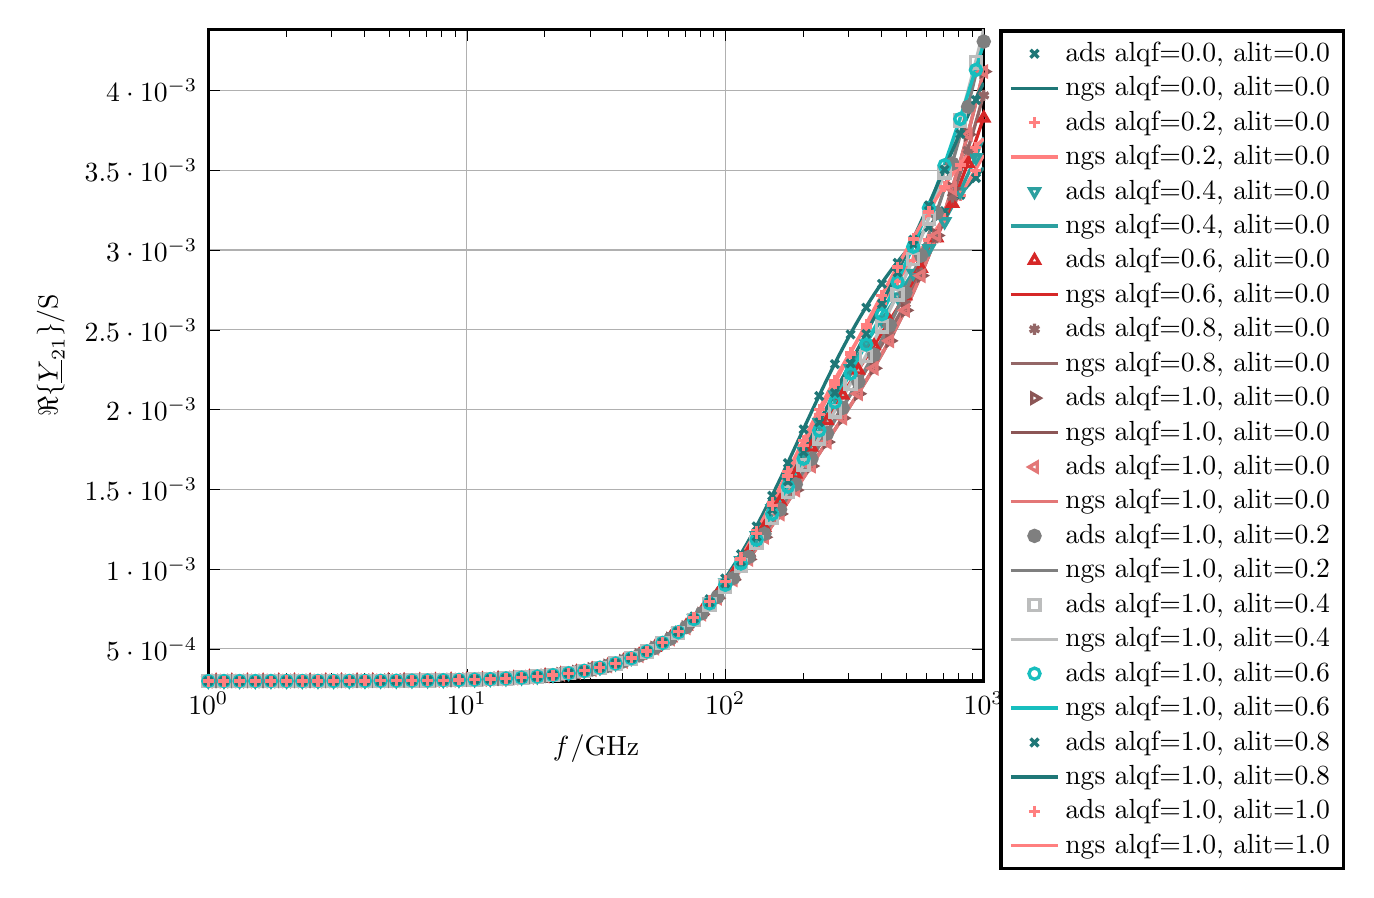
\begin{tikzpicture}[font=\normalsize]
\pgfplotsset{every axis/.append style={very thick}},
\definecolor{color0}{rgb}{0.12157, 0.46667, 0.46667}
\definecolor{color1}{rgb}{1.00000, 0.49804, 0.49804}
\definecolor{color2}{rgb}{0.17255, 0.62745, 0.62745}
\definecolor{color3}{rgb}{0.83922, 0.15294, 0.15294}
\definecolor{color4}{rgb}{0.58039, 0.40392, 0.40392}
\definecolor{color5}{rgb}{0.54902, 0.33725, 0.33725}
\definecolor{color6}{rgb}{0.89020, 0.46667, 0.46667}
\definecolor{color7}{rgb}{0.49804, 0.49804, 0.49804}
\definecolor{color8}{rgb}{0.73725, 0.74118, 0.74118}
\definecolor{color9}{rgb}{0.09020, 0.74510, 0.74510}

\begin{axis}[
width=4.5in,
xlabel={$f_{\mathrm{}}^{}/\si{\giga\hertz}$},
ylabel={$\Re\{\underline{Y}_{\mathrm{21}}^{}\}/\si{\siemens}$},
xmode=log,
% xmin=0,
% xmax=0,
% restrict x to domain=0:1,
log basis x=10,
% ymin=0,
% ymax=0,
% restrict y to domain=0:1,
log basis y=10,
xmajorgrids,
enlargelimits=false,
scaled ticks=false,
ymajorgrids,
x tick style={color=black},
y tick style={color=black},
x grid style={white!69.01960784313725!black},
y grid style={white!69.01960784313725!black},
/tikz/mark repeat=2,
legend style={at={(1.02,1.00)}, anchor=north west,legend cell align=left, align=left},
]
\addplot [color=color0, only marks, mark=x, mark options={solid}, mark phase=0, ]
  table[row sep=crcr, x expr=\thisrowno{0}*1.000000e-09, y expr=\thisrowno{1}*1.000000e+00]{
1e+09 0.000298566\\
1.07227e+09 0.000298578\\
1.14976e+09 0.000298591\\
1.23285e+09 0.000298607\\
1.32194e+09 0.000298625\\
1.41747e+09 0.000298646\\
1.51991e+09 0.00029867\\
1.62975e+09 0.000298697\\
1.74753e+09 0.000298729\\
1.87382e+09 0.000298765\\
2.00923e+09 0.000298807\\
2.15443e+09 0.000298856\\
2.31013e+09 0.000298911\\
2.47708e+09 0.000298975\\
2.65609e+09 0.000299049\\
2.84804e+09 0.000299134\\
3.05386e+09 0.000299232\\
3.27455e+09 0.000299344\\
3.51119e+09 0.000299474\\
3.76494e+09 0.000299623\\
4.03702e+09 0.000299795\\
4.32876e+09 0.000299993\\
4.64159e+09 0.00030022\\
4.97702e+09 0.000300482\\
5.3367e+09 0.000300784\\
5.72237e+09 0.00030113\\
6.13591e+09 0.000301529\\
6.57933e+09 0.000301988\\
7.0548e+09 0.000302515\\
7.56463e+09 0.000303122\\
8.11131e+09 0.000303819\\
8.69749e+09 0.000304621\\
9.32603e+09 0.000305543\\
1e+10 0.000306602\\
1.07227e+10 0.000307819\\
1.14976e+10 0.000309217\\
1.23285e+10 0.000310823\\
1.32194e+10 0.000312667\\
1.41747e+10 0.000314785\\
1.51991e+10 0.000317217\\
1.62975e+10 0.000320008\\
1.74753e+10 0.000323211\\
1.87382e+10 0.000326885\\
2.00923e+10 0.000331098\\
2.15443e+10 0.000335928\\
2.31013e+10 0.000341461\\
2.47708e+10 0.000347798\\
2.65609e+10 0.00035505\\
2.84804e+10 0.000363345\\
3.05386e+10 0.000372824\\
3.27455e+10 0.000383648\\
3.51119e+10 0.000395994\\
3.76494e+10 0.000410061\\
4.03702e+10 0.000426068\\
4.32876e+10 0.000444254\\
4.64159e+10 0.000464882\\
4.97702e+10 0.000488235\\
5.3367e+10 0.000514616\\
5.72237e+10 0.000544343\\
6.13591e+10 0.00057775\\
6.57933e+10 0.000615176\\
7.0548e+10 0.000656958\\
7.56463e+10 0.000703424\\
8.11131e+10 0.000754877\\
8.69749e+10 0.000811582\\
9.32603e+10 0.000873748\\
1e+11 0.000941513\\
1.07227e+11 0.00101492\\
1.14976e+11 0.0010939\\
1.23285e+11 0.00117827\\
1.32194e+11 0.00126771\\
1.41747e+11 0.00136173\\
1.51991e+11 0.00145975\\
1.62975e+11 0.00156103\\
1.74753e+11 0.00166472\\
1.87382e+11 0.00176991\\
2.00923e+11 0.00187564\\
2.15443e+11 0.00198093\\
2.31013e+11 0.00208483\\
2.47708e+11 0.00218649\\
2.65609e+11 0.00228513\\
2.84804e+11 0.00238012\\
3.05386e+11 0.00247095\\
3.27455e+11 0.00255729\\
3.51119e+11 0.00263894\\
3.76494e+11 0.00271587\\
4.03702e+11 0.00278817\\
4.32876e+11 0.00285606\\
4.64159e+11 0.00291986\\
4.97702e+11 0.00297998\\
5.3367e+11 0.0030369\\
5.72237e+11 0.00309118\\
6.13591e+11 0.00314341\\
6.57933e+11 0.00319423\\
7.0548e+11 0.00324431\\
7.56463e+11 0.00329434\\
8.11131e+11 0.00334505\\
8.69749e+11 0.00339717\\
9.32603e+11 0.00345144\\
1e+12 0.00350864\\
};
\addlegendentry{ads alqf=0.0, alit=0.0}
\addplot [color=color0, solid,  mark phase=0, ]
  table[row sep=crcr, x expr=\thisrowno{0}*1.000000e-09, y expr=\thisrowno{1}*1.000000e+00]{
1e+09 0.000298566\\
1.02306e+09 0.00029857\\
1.04665e+09 0.000298574\\
1.07079e+09 0.000298578\\
1.09548e+09 0.000298582\\
1.12074e+09 0.000298586\\
1.14658e+09 0.000298591\\
1.17302e+09 0.000298596\\
1.20007e+09 0.000298601\\
1.22775e+09 0.000298606\\
1.25606e+09 0.000298612\\
1.28502e+09 0.000298618\\
1.31466e+09 0.000298624\\
1.34497e+09 0.00029863\\
1.37599e+09 0.000298637\\
1.40772e+09 0.000298644\\
1.44018e+09 0.000298651\\
1.47339e+09 0.000298659\\
1.50736e+09 0.000298667\\
1.54212e+09 0.000298676\\
1.57768e+09 0.000298684\\
1.61406e+09 0.000298694\\
1.65128e+09 0.000298703\\
1.68936e+09 0.000298713\\
1.72832e+09 0.000298724\\
1.76817e+09 0.000298735\\
1.80895e+09 0.000298747\\
1.85066e+09 0.000298759\\
1.89334e+09 0.000298772\\
1.937e+09 0.000298785\\
1.98166e+09 0.000298799\\
2.02736e+09 0.000298814\\
2.07411e+09 0.000298829\\
2.12194e+09 0.000298845\\
2.17087e+09 0.000298862\\
2.22093e+09 0.00029888\\
2.27214e+09 0.000298898\\
2.32454e+09 0.000298917\\
2.37814e+09 0.000298938\\
2.43298e+09 0.000298959\\
2.48908e+09 0.000298981\\
2.54648e+09 0.000299004\\
2.6052e+09 0.000299029\\
2.66528e+09 0.000299054\\
2.72674e+09 0.000299081\\
2.78962e+09 0.000299109\\
2.85394e+09 0.000299138\\
2.91976e+09 0.000299169\\
2.98708e+09 0.000299201\\
3.05597e+09 0.000299234\\
3.12644e+09 0.00029927\\
3.19853e+09 0.000299306\\
3.27229e+09 0.000299345\\
3.34775e+09 0.000299385\\
3.42494e+09 0.000299428\\
3.50392e+09 0.000299472\\
3.58472e+09 0.000299518\\
3.66738e+09 0.000299567\\
3.75195e+09 0.000299618\\
3.83847e+09 0.000299671\\
3.92699e+09 0.000299727\\
4.01754e+09 0.000299785\\
4.11019e+09 0.000299846\\
4.20496e+09 0.00029991\\
4.30193e+09 0.000299977\\
4.40113e+09 0.000300047\\
4.50262e+09 0.000300121\\
4.60645e+09 0.000300198\\
4.71267e+09 0.000300278\\
4.82135e+09 0.000300363\\
4.93253e+09 0.000300451\\
5.04627e+09 0.000300543\\
5.16263e+09 0.00030064\\
5.28168e+09 0.000300741\\
5.40348e+09 0.000300847\\
5.52808e+09 0.000300958\\
5.65556e+09 0.000301074\\
5.78597e+09 0.000301196\\
5.91939e+09 0.000301323\\
6.05589e+09 0.000301457\\
6.19554e+09 0.000301596\\
6.33841e+09 0.000301742\\
6.48457e+09 0.000301895\\
6.6341e+09 0.000302055\\
6.78708e+09 0.000302223\\
6.94359e+09 0.000302398\\
7.10371e+09 0.000302581\\
7.26752e+09 0.000302774\\
7.43511e+09 0.000302975\\
7.60656e+09 0.000303185\\
7.78196e+09 0.000303405\\
7.96141e+09 0.000303636\\
8.145e+09 0.000303877\\
8.33282e+09 0.000304129\\
8.52497e+09 0.000304393\\
8.72156e+09 0.00030467\\
8.92267e+09 0.000304959\\
9.12843e+09 0.000305262\\
9.33893e+09 0.000305579\\
9.55428e+09 0.000305911\\
9.7746e+09 0.000306258\\
1e+10 0.000306621\\
1.02306e+10 0.000307001\\
1.04665e+10 0.000307399\\
1.07079e+10 0.000307815\\
1.09548e+10 0.00030825\\
1.12074e+10 0.000308706\\
1.14658e+10 0.000309183\\
1.17302e+10 0.000309682\\
1.20007e+10 0.000310204\\
1.22775e+10 0.00031075\\
1.25606e+10 0.000311322\\
1.28502e+10 0.00031192\\
1.31466e+10 0.000312545\\
1.34497e+10 0.0003132\\
1.37599e+10 0.000313884\\
1.40772e+10 0.000314601\\
1.44018e+10 0.00031535\\
1.47339e+10 0.000316134\\
1.50736e+10 0.000316954\\
1.54212e+10 0.000317812\\
1.57768e+10 0.00031871\\
1.61406e+10 0.000319648\\
1.65128e+10 0.00032063\\
1.68936e+10 0.000321657\\
1.72832e+10 0.000322732\\
1.76817e+10 0.000323855\\
1.80895e+10 0.00032503\\
1.85066e+10 0.000326259\\
1.89334e+10 0.000327544\\
1.937e+10 0.000328888\\
1.98166e+10 0.000330293\\
2.02736e+10 0.000331763\\
2.07411e+10 0.000333299\\
2.12194e+10 0.000334906\\
2.17087e+10 0.000336585\\
2.22093e+10 0.000338341\\
2.27214e+10 0.000340177\\
2.32454e+10 0.000342095\\
2.37814e+10 0.000344101\\
2.43298e+10 0.000346197\\
2.48908e+10 0.000348388\\
2.54648e+10 0.000350678\\
2.6052e+10 0.000353071\\
2.66528e+10 0.000355571\\
2.72674e+10 0.000358183\\
2.78962e+10 0.000360913\\
2.85394e+10 0.000363764\\
2.91976e+10 0.000366742\\
2.98708e+10 0.000369853\\
3.05597e+10 0.000373102\\
3.12644e+10 0.000376495\\
3.19853e+10 0.000380038\\
3.27229e+10 0.000383736\\
3.34775e+10 0.000387598\\
3.42494e+10 0.000391629\\
3.50392e+10 0.000395836\\
3.58472e+10 0.000400226\\
3.66738e+10 0.000404807\\
3.75195e+10 0.000409586\\
3.83847e+10 0.000414571\\
3.92699e+10 0.000419771\\
4.01754e+10 0.000425193\\
4.11019e+10 0.000430846\\
4.20496e+10 0.00043674\\
4.30193e+10 0.000442882\\
4.40113e+10 0.000449283\\
4.50262e+10 0.000455953\\
4.60645e+10 0.0004629\\
4.71267e+10 0.000470135\\
4.82135e+10 0.000477669\\
4.93253e+10 0.000485511\\
5.04627e+10 0.000493673\\
5.16263e+10 0.000502166\\
5.28168e+10 0.000511\\
5.40348e+10 0.000520187\\
5.52808e+10 0.000529738\\
5.65556e+10 0.000539665\\
5.78597e+10 0.000549979\\
5.91939e+10 0.000560693\\
6.05589e+10 0.000571819\\
6.19554e+10 0.000583367\\
6.33841e+10 0.000595351\\
6.48457e+10 0.000607781\\
6.6341e+10 0.00062067\\
6.78708e+10 0.00063403\\
6.94359e+10 0.000647872\\
7.10371e+10 0.000662208\\
7.26752e+10 0.000677048\\
7.43511e+10 0.000692404\\
7.60656e+10 0.000708286\\
7.78196e+10 0.000724704\\
7.96141e+10 0.000741669\\
8.145e+10 0.000759189\\
8.33282e+10 0.000777273\\
8.52497e+10 0.000795928\\
8.72156e+10 0.000815163\\
8.92267e+10 0.000834984\\
9.12843e+10 0.000855396\\
9.33893e+10 0.000876404\\
9.55428e+10 0.000898012\\
9.7746e+10 0.000920223\\
1e+11 0.000943037\\
1.02306e+11 0.000966457\\
1.04665e+11 0.00099048\\
1.07079e+11 0.0010151\\
1.09548e+11 0.00104033\\
1.12074e+11 0.00106614\\
1.14658e+11 0.00109255\\
1.17302e+11 0.00111953\\
1.20007e+11 0.00114708\\
1.22775e+11 0.00117518\\
1.25606e+11 0.00120384\\
1.28502e+11 0.00123302\\
1.31466e+11 0.00126272\\
1.34497e+11 0.00129292\\
1.37599e+11 0.00132359\\
1.40772e+11 0.00135472\\
1.44018e+11 0.00138629\\
1.47339e+11 0.00141827\\
1.50736e+11 0.00145063\\
1.54212e+11 0.00148335\\
1.57768e+11 0.00151641\\
1.61406e+11 0.00154977\\
1.65128e+11 0.0015834\\
1.68936e+11 0.00161727\\
1.72832e+11 0.00165135\\
1.76817e+11 0.0016856\\
1.80895e+11 0.00172\\
1.85066e+11 0.00175452\\
1.89334e+11 0.0017891\\
1.937e+11 0.00182373\\
1.98166e+11 0.00185836\\
2.02736e+11 0.00189297\\
2.07411e+11 0.00192752\\
2.12194e+11 0.00196197\\
2.17087e+11 0.0019963\\
2.22093e+11 0.00203047\\
2.27214e+11 0.00206445\\
2.32454e+11 0.0020982\\
2.37814e+11 0.00213171\\
2.43298e+11 0.00216494\\
2.48908e+11 0.00219787\\
2.54648e+11 0.00223047\\
2.6052e+11 0.00226272\\
2.66528e+11 0.00229459\\
2.72674e+11 0.00232607\\
2.78962e+11 0.00235713\\
2.85394e+11 0.00238776\\
2.91976e+11 0.00241794\\
2.98708e+11 0.00244767\\
3.05597e+11 0.00247692\\
3.12644e+11 0.00250569\\
3.19853e+11 0.00253396\\
3.27229e+11 0.00256174\\
3.34775e+11 0.00258902\\
3.42494e+11 0.0026158\\
3.50392e+11 0.00264206\\
3.58472e+11 0.00266782\\
3.66738e+11 0.00269308\\
3.75195e+11 0.00271783\\
3.83847e+11 0.00274209\\
3.92699e+11 0.00276586\\
4.01754e+11 0.00278914\\
4.11019e+11 0.00281195\\
4.20496e+11 0.00283429\\
4.30193e+11 0.00285618\\
4.40113e+11 0.00287762\\
4.50262e+11 0.00289864\\
4.60645e+11 0.00291925\\
4.71267e+11 0.00293945\\
4.82135e+11 0.00295927\\
4.93253e+11 0.00297873\\
5.04627e+11 0.00299784\\
5.16263e+11 0.00301661\\
5.28168e+11 0.00303508\\
5.40348e+11 0.00305325\\
5.52808e+11 0.00307115\\
5.65556e+11 0.0030888\\
5.78597e+11 0.00310622\\
5.91939e+11 0.00312343\\
6.05589e+11 0.00314045\\
6.19554e+11 0.00315731\\
6.33841e+11 0.00317402\\
6.48457e+11 0.00319062\\
6.6341e+11 0.00320713\\
6.78708e+11 0.00322356\\
6.94359e+11 0.00323995\\
7.10371e+11 0.00325632\\
7.26752e+11 0.00327269\\
7.43511e+11 0.00328909\\
7.60656e+11 0.00330554\\
7.78196e+11 0.00332206\\
7.96141e+11 0.0033387\\
8.145e+11 0.00335546\\
8.33282e+11 0.00337238\\
8.52497e+11 0.00338948\\
8.72156e+11 0.00340679\\
8.92267e+11 0.00342433\\
9.12843e+11 0.00344214\\
9.33893e+11 0.00346023\\
9.55428e+11 0.00347864\\
9.7746e+11 0.00349739\\
1e+12 0.00351651\\
};
\addlegendentry{ngs alqf=0.0, alit=0.0}
\addplot [color=color1, only marks, mark=+, mark options={solid}, mark phase=0, ]
  table[row sep=crcr, x expr=\thisrowno{0}*1.000000e-09, y expr=\thisrowno{1}*1.000000e+00]{
1e+09 0.000298566\\
1.07227e+09 0.000298578\\
1.14976e+09 0.000298591\\
1.23285e+09 0.000298607\\
1.32194e+09 0.000298625\\
1.41747e+09 0.000298646\\
1.51991e+09 0.000298669\\
1.62975e+09 0.000298697\\
1.74753e+09 0.000298728\\
1.87382e+09 0.000298765\\
2.00923e+09 0.000298807\\
2.15443e+09 0.000298855\\
2.31013e+09 0.00029891\\
2.47708e+09 0.000298974\\
2.65609e+09 0.000299048\\
2.84804e+09 0.000299132\\
3.05386e+09 0.00029923\\
3.27455e+09 0.000299342\\
3.51119e+09 0.000299472\\
3.76494e+09 0.00029962\\
4.03702e+09 0.000299792\\
4.32876e+09 0.000299989\\
4.64159e+09 0.000300216\\
4.97702e+09 0.000300477\\
5.3367e+09 0.000300778\\
5.72237e+09 0.000301124\\
6.13591e+09 0.000301522\\
6.57933e+09 0.00030198\\
7.0548e+09 0.000302506\\
7.56463e+09 0.000303111\\
8.11131e+09 0.000303807\\
8.69749e+09 0.000304606\\
9.32603e+09 0.000305525\\
1e+10 0.000306581\\
1.07227e+10 0.000307795\\
1.14976e+10 0.000309189\\
1.23285e+10 0.00031079\\
1.32194e+10 0.000312629\\
1.41747e+10 0.000314741\\
1.51991e+10 0.000317164\\
1.62975e+10 0.000319946\\
1.74753e+10 0.000323137\\
1.87382e+10 0.000326797\\
2.00923e+10 0.000330992\\
2.15443e+10 0.000335801\\
2.31013e+10 0.000341308\\
2.47708e+10 0.000347612\\
2.65609e+10 0.000354825\\
2.84804e+10 0.00036307\\
3.05386e+10 0.000372487\\
3.27455e+10 0.000383234\\
3.51119e+10 0.000395484\\
3.76494e+10 0.000409429\\
4.03702e+10 0.000425283\\
4.32876e+10 0.000443277\\
4.64159e+10 0.000463662\\
4.97702e+10 0.00048671\\
5.3367e+10 0.000512707\\
5.72237e+10 0.000541952\\
6.13591e+10 0.000574755\\
6.57933e+10 0.000611427\\
7.0548e+10 0.000652272\\
7.56463e+10 0.000697578\\
8.11131e+10 0.000747605\\
8.69749e+10 0.000802566\\
9.32603e+10 0.000862618\\
1e+11 0.00092784\\
1.07227e+11 0.00099822\\
1.14976e+11 0.00107364\\
1.23285e+11 0.00115386\\
1.32194e+11 0.00123852\\
1.41747e+11 0.00132714\\
1.51991e+11 0.00141912\\
1.62975e+11 0.00151376\\
1.74753e+11 0.00161029\\
1.87382e+11 0.00170788\\
2.00923e+11 0.0018057\\
2.15443e+11 0.00190293\\
2.31013e+11 0.00199883\\
2.47708e+11 0.00209272\\
2.65609e+11 0.00218406\\
2.84804e+11 0.00227244\\
3.05386e+11 0.00235757\\
3.27455e+11 0.00243934\\
3.51119e+11 0.00251775\\
3.76494e+11 0.00259295\\
4.03702e+11 0.00266521\\
4.32876e+11 0.00273489\\
4.64159e+11 0.00280246\\
4.97702e+11 0.00286844\\
5.3367e+11 0.00293344\\
5.72237e+11 0.00299808\\
6.13591e+11 0.00306305\\
6.57933e+11 0.00312905\\
7.0548e+11 0.0031968\\
7.56463e+11 0.00326705\\
8.11131e+11 0.00334054\\
8.69749e+11 0.00341804\\
9.32603e+11 0.00350032\\
1e+12 0.00358815\\
};
\addlegendentry{ads alqf=0.2, alit=0.0}
\addplot [color=color1, solid,  mark phase=0, ]
  table[row sep=crcr, x expr=\thisrowno{0}*1.000000e-09, y expr=\thisrowno{1}*1.000000e+00]{
1e+09 0.000298566\\
1.02306e+09 0.00029857\\
1.04665e+09 0.000298573\\
1.07079e+09 0.000298577\\
1.09548e+09 0.000298582\\
1.12074e+09 0.000298586\\
1.14658e+09 0.000298591\\
1.17302e+09 0.000298596\\
1.20007e+09 0.000298601\\
1.22775e+09 0.000298606\\
1.25606e+09 0.000298612\\
1.28502e+09 0.000298617\\
1.31466e+09 0.000298623\\
1.34497e+09 0.00029863\\
1.37599e+09 0.000298637\\
1.40772e+09 0.000298644\\
1.44018e+09 0.000298651\\
1.47339e+09 0.000298659\\
1.50736e+09 0.000298667\\
1.54212e+09 0.000298675\\
1.57768e+09 0.000298684\\
1.61406e+09 0.000298693\\
1.65128e+09 0.000298703\\
1.68936e+09 0.000298713\\
1.72832e+09 0.000298724\\
1.76817e+09 0.000298735\\
1.80895e+09 0.000298746\\
1.85066e+09 0.000298758\\
1.89334e+09 0.000298771\\
1.937e+09 0.000298784\\
1.98166e+09 0.000298798\\
2.02736e+09 0.000298813\\
2.07411e+09 0.000298828\\
2.12194e+09 0.000298844\\
2.17087e+09 0.000298861\\
2.22093e+09 0.000298879\\
2.27214e+09 0.000298897\\
2.32454e+09 0.000298916\\
2.37814e+09 0.000298937\\
2.43298e+09 0.000298958\\
2.48908e+09 0.00029898\\
2.54648e+09 0.000299003\\
2.6052e+09 0.000299027\\
2.66528e+09 0.000299053\\
2.72674e+09 0.000299079\\
2.78962e+09 0.000299107\\
2.85394e+09 0.000299137\\
2.91976e+09 0.000299167\\
2.98708e+09 0.000299199\\
3.05597e+09 0.000299233\\
3.12644e+09 0.000299268\\
3.19853e+09 0.000299304\\
3.27229e+09 0.000299343\\
3.34775e+09 0.000299383\\
3.42494e+09 0.000299425\\
3.50392e+09 0.00029947\\
3.58472e+09 0.000299516\\
3.66738e+09 0.000299564\\
3.75195e+09 0.000299615\\
3.83847e+09 0.000299668\\
3.92699e+09 0.000299724\\
4.01754e+09 0.000299782\\
4.11019e+09 0.000299843\\
4.20496e+09 0.000299907\\
4.30193e+09 0.000299974\\
4.40113e+09 0.000300044\\
4.50262e+09 0.000300117\\
4.60645e+09 0.000300194\\
4.71267e+09 0.000300274\\
4.82135e+09 0.000300358\\
4.93253e+09 0.000300446\\
5.04627e+09 0.000300538\\
5.16263e+09 0.000300635\\
5.28168e+09 0.000300736\\
5.40348e+09 0.000300842\\
5.52808e+09 0.000300952\\
5.65556e+09 0.000301068\\
5.78597e+09 0.00030119\\
5.91939e+09 0.000301317\\
6.05589e+09 0.00030145\\
6.19554e+09 0.000301589\\
6.33841e+09 0.000301735\\
6.48457e+09 0.000301887\\
6.6341e+09 0.000302047\\
6.78708e+09 0.000302214\\
6.94359e+09 0.000302389\\
7.10371e+09 0.000302572\\
7.26752e+09 0.000302763\\
7.43511e+09 0.000302964\\
7.60656e+09 0.000303174\\
7.78196e+09 0.000303393\\
7.96141e+09 0.000303623\\
8.145e+09 0.000303864\\
8.33282e+09 0.000304115\\
8.52497e+09 0.000304379\\
8.72156e+09 0.000304655\\
8.92267e+09 0.000304943\\
9.12843e+09 0.000305245\\
9.33893e+09 0.000305561\\
9.55428e+09 0.000305892\\
9.7746e+09 0.000306238\\
1e+10 0.000306601\\
1.02306e+10 0.00030698\\
1.04665e+10 0.000307376\\
1.07079e+10 0.000307791\\
1.09548e+10 0.000308225\\
1.12074e+10 0.00030868\\
1.14658e+10 0.000309155\\
1.17302e+10 0.000309653\\
1.20007e+10 0.000310173\\
1.22775e+10 0.000310718\\
1.25606e+10 0.000311288\\
1.28502e+10 0.000311884\\
1.31466e+10 0.000312507\\
1.34497e+10 0.00031316\\
1.37599e+10 0.000313842\\
1.40772e+10 0.000314556\\
1.44018e+10 0.000315303\\
1.47339e+10 0.000316085\\
1.50736e+10 0.000316902\\
1.54212e+10 0.000317757\\
1.57768e+10 0.000318651\\
1.61406e+10 0.000319587\\
1.65128e+10 0.000320565\\
1.68936e+10 0.000321589\\
1.72832e+10 0.000322659\\
1.76817e+10 0.000323778\\
1.80895e+10 0.000324949\\
1.85066e+10 0.000326173\\
1.89334e+10 0.000327453\\
1.937e+10 0.000328791\\
1.98166e+10 0.00033019\\
2.02736e+10 0.000331654\\
2.07411e+10 0.000333183\\
2.12194e+10 0.000334783\\
2.17087e+10 0.000336455\\
2.22093e+10 0.000338202\\
2.27214e+10 0.000340029\\
2.32454e+10 0.000341939\\
2.37814e+10 0.000343934\\
2.43298e+10 0.00034602\\
2.48908e+10 0.000348199\\
2.54648e+10 0.000350477\\
2.6052e+10 0.000352856\\
2.66528e+10 0.000355342\\
2.72674e+10 0.000357939\\
2.78962e+10 0.000360652\\
2.85394e+10 0.000363486\\
2.91976e+10 0.000366445\\
2.98708e+10 0.000369536\\
3.05597e+10 0.000372763\\
3.12644e+10 0.000376132\\
3.19853e+10 0.00037965\\
3.27229e+10 0.000383321\\
3.34775e+10 0.000387153\\
3.42494e+10 0.000391153\\
3.50392e+10 0.000395326\\
3.58472e+10 0.000399679\\
3.66738e+10 0.00040422\\
3.75195e+10 0.000408957\\
3.83847e+10 0.000413897\\
3.92699e+10 0.000419047\\
4.01754e+10 0.000424416\\
4.11019e+10 0.000430012\\
4.20496e+10 0.000435843\\
4.30193e+10 0.000441919\\
4.40113e+10 0.000448249\\
4.50262e+10 0.00045484\\
4.60645e+10 0.000461704\\
4.71267e+10 0.000468849\\
4.82135e+10 0.000476286\\
4.93253e+10 0.000484023\\
5.04627e+10 0.000492072\\
5.16263e+10 0.000500443\\
5.28168e+10 0.000509146\\
5.40348e+10 0.000518192\\
5.52808e+10 0.000527591\\
5.65556e+10 0.000537354\\
5.78597e+10 0.000547492\\
5.91939e+10 0.000558017\\
6.05589e+10 0.000568938\\
6.19554e+10 0.000580267\\
6.33841e+10 0.000592014\\
6.48457e+10 0.000604191\\
6.6341e+10 0.000616808\\
6.78708e+10 0.000629875\\
6.94359e+10 0.000643403\\
7.10371e+10 0.000657402\\
7.26752e+10 0.000671881\\
7.43511e+10 0.000686851\\
7.60656e+10 0.000702319\\
7.78196e+10 0.000718294\\
7.96141e+10 0.000734785\\
8.145e+10 0.000751799\\
8.33282e+10 0.000769343\\
8.52497e+10 0.000787423\\
8.72156e+10 0.000806043\\
8.92267e+10 0.00082521\\
9.12843e+10 0.000844926\\
9.33893e+10 0.000865195\\
9.55428e+10 0.000886017\\
9.7746e+10 0.000907394\\
1e+11 0.000929326\\
1.02306e+11 0.00095181\\
1.04665e+11 0.000974844\\
1.07079e+11 0.000998424\\
1.09548e+11 0.00102254\\
1.12074e+11 0.0010472\\
1.14658e+11 0.00107238\\
1.17302e+11 0.00109807\\
1.20007e+11 0.00112427\\
1.22775e+11 0.00115097\\
1.25606e+11 0.00117814\\
1.28502e+11 0.00120578\\
1.31466e+11 0.00123386\\
1.34497e+11 0.00126237\\
1.37599e+11 0.00129129\\
1.40772e+11 0.00132061\\
1.44018e+11 0.00135028\\
1.47339e+11 0.00138031\\
1.50736e+11 0.00141065\\
1.54212e+11 0.00144128\\
1.57768e+11 0.00147219\\
1.61406e+11 0.00150334\\
1.65128e+11 0.0015347\\
1.68936e+11 0.00156625\\
1.72832e+11 0.00159795\\
1.76817e+11 0.00162978\\
1.80895e+11 0.00166171\\
1.85066e+11 0.00169371\\
1.89334e+11 0.00172575\\
1.937e+11 0.0017578\\
1.98166e+11 0.00178984\\
2.02736e+11 0.00182182\\
2.07411e+11 0.00185374\\
2.12194e+11 0.00188555\\
2.17087e+11 0.00191724\\
2.22093e+11 0.00194877\\
2.27214e+11 0.00198013\\
2.32454e+11 0.00201129\\
2.37814e+11 0.00204223\\
2.43298e+11 0.00207292\\
2.48908e+11 0.00210336\\
2.54648e+11 0.00213352\\
2.6052e+11 0.00216338\\
2.66528e+11 0.00219294\\
2.72674e+11 0.00222218\\
2.78962e+11 0.00225109\\
2.85394e+11 0.00227965\\
2.91976e+11 0.00230787\\
2.98708e+11 0.00233573\\
3.05597e+11 0.00236324\\
3.12644e+11 0.00239038\\
3.19853e+11 0.00241716\\
3.27229e+11 0.00244358\\
3.34775e+11 0.00246963\\
3.42494e+11 0.00249533\\
3.50392e+11 0.00252068\\
3.58472e+11 0.00254569\\
3.66738e+11 0.00257036\\
3.75195e+11 0.0025947\\
3.83847e+11 0.00261872\\
3.92699e+11 0.00264244\\
4.01754e+11 0.00266586\\
4.11019e+11 0.00268901\\
4.20496e+11 0.00271189\\
4.30193e+11 0.00273452\\
4.40113e+11 0.00275693\\
4.50262e+11 0.00277911\\
4.60645e+11 0.00280111\\
4.71267e+11 0.00282293\\
4.82135e+11 0.00284459\\
4.93253e+11 0.00286611\\
5.04627e+11 0.00288753\\
5.16263e+11 0.00290884\\
5.28168e+11 0.00293009\\
5.40348e+11 0.00295129\\
5.52808e+11 0.00297247\\
5.65556e+11 0.00299364\\
5.78597e+11 0.00301484\\
5.91939e+11 0.00303609\\
6.05589e+11 0.0030574\\
6.19554e+11 0.00307881\\
6.33841e+11 0.00310034\\
6.48457e+11 0.00312202\\
6.6341e+11 0.00314387\\
6.78708e+11 0.00316592\\
6.94359e+11 0.00318819\\
7.10371e+11 0.00321071\\
7.26752e+11 0.0032335\\
7.43511e+11 0.0032566\\
7.60656e+11 0.00328002\\
7.78196e+11 0.0033038\\
7.96141e+11 0.00332795\\
8.145e+11 0.00335252\\
8.33282e+11 0.00337752\\
8.52497e+11 0.00340298\\
8.72156e+11 0.00342893\\
8.92267e+11 0.0034554\\
9.12843e+11 0.0034824\\
9.33893e+11 0.00350998\\
9.55428e+11 0.00353815\\
9.7746e+11 0.00356695\\
1e+12 0.0035964\\
};
\addlegendentry{ngs alqf=0.2, alit=0.0}
\addplot [color=color2, only marks, mark=triangle, mark options={solid, rotate=180}, mark phase=0, ]
  table[row sep=crcr, x expr=\thisrowno{0}*1.000000e-09, y expr=\thisrowno{1}*1.000000e+00]{
1e+09 0.000298566\\
1.07227e+09 0.000298577\\
1.14976e+09 0.000298591\\
1.23285e+09 0.000298607\\
1.32194e+09 0.000298625\\
1.41747e+09 0.000298645\\
1.51991e+09 0.000298669\\
1.62975e+09 0.000298696\\
1.74753e+09 0.000298728\\
1.87382e+09 0.000298764\\
2.00923e+09 0.000298806\\
2.15443e+09 0.000298854\\
2.31013e+09 0.000298909\\
2.47708e+09 0.000298973\\
2.65609e+09 0.000299046\\
2.84804e+09 0.000299131\\
3.05386e+09 0.000299228\\
3.27455e+09 0.00029934\\
3.51119e+09 0.000299469\\
3.76494e+09 0.000299618\\
4.03702e+09 0.000299789\\
4.32876e+09 0.000299986\\
4.64159e+09 0.000300212\\
4.97702e+09 0.000300473\\
5.3367e+09 0.000300773\\
5.72237e+09 0.000301118\\
6.13591e+09 0.000301515\\
6.57933e+09 0.000301971\\
7.0548e+09 0.000302496\\
7.56463e+09 0.0003031\\
8.11131e+09 0.000303794\\
8.69749e+09 0.000304591\\
9.32603e+09 0.000305508\\
1e+10 0.000306561\\
1.07227e+10 0.000307771\\
1.14976e+10 0.000309161\\
1.23285e+10 0.000310758\\
1.32194e+10 0.000312591\\
1.41747e+10 0.000314695\\
1.51991e+10 0.000317111\\
1.62975e+10 0.000319882\\
1.74753e+10 0.000323062\\
1.87382e+10 0.000326707\\
2.00923e+10 0.000330885\\
2.15443e+10 0.000335672\\
2.31013e+10 0.000341152\\
2.47708e+10 0.000347424\\
2.65609e+10 0.000354595\\
2.84804e+10 0.00036279\\
3.05386e+10 0.000372144\\
3.27455e+10 0.000382811\\
3.51119e+10 0.000394962\\
3.76494e+10 0.000408782\\
4.03702e+10 0.000424479\\
4.32876e+10 0.000442276\\
4.64159e+10 0.000462414\\
4.97702e+10 0.00048515\\
5.3367e+10 0.000510756\\
5.72237e+10 0.000539511\\
6.13591e+10 0.000571702\\
6.57933e+10 0.000607612\\
7.0548e+10 0.000647514\\
7.56463e+10 0.000691658\\
8.11131e+10 0.000740261\\
8.69749e+10 0.000793493\\
9.32603e+10 0.00085146\\
1e+11 0.000914194\\
1.07227e+11 0.000981633\\
1.14976e+11 0.00105362\\
1.23285e+11 0.00112988\\
1.32194e+11 0.00121003\\
1.41747e+11 0.00129359\\
1.51991e+11 0.00137999\\
1.62975e+11 0.00146858\\
1.74753e+11 0.00155865\\
1.87382e+11 0.00164949\\
2.00923e+11 0.00174039\\
2.15443e+11 0.00183072\\
2.31013e+11 0.00191988\\
2.47708e+11 0.00200742\\
2.65609e+11 0.00209296\\
2.84804e+11 0.0021763\\
3.05386e+11 0.00225736\\
3.27455e+11 0.0023362\\
3.51119e+11 0.002413\\
3.76494e+11 0.00248808\\
4.03702e+11 0.00256184\\
4.32876e+11 0.00263479\\
4.64159e+11 0.00270752\\
4.97702e+11 0.00278066\\
5.3367e+11 0.0028549\\
5.72237e+11 0.00293097\\
6.13591e+11 0.00300961\\
6.57933e+11 0.0030916\\
7.0548e+11 0.00317772\\
7.56463e+11 0.00326874\\
8.11131e+11 0.00336546\\
8.69749e+11 0.00346865\\
9.32603e+11 0.0035791\\
1e+12 0.00369757\\
};
\addlegendentry{ads alqf=0.4, alit=0.0}
\addplot [color=color2, solid,  mark phase=0, ]
  table[row sep=crcr, x expr=\thisrowno{0}*1.000000e-09, y expr=\thisrowno{1}*1.000000e+00]{
1e+09 0.000298566\\
1.02306e+09 0.000298569\\
1.04665e+09 0.000298573\\
1.07079e+09 0.000298577\\
1.09548e+09 0.000298581\\
1.12074e+09 0.000298586\\
1.14658e+09 0.00029859\\
1.17302e+09 0.000298595\\
1.20007e+09 0.0002986\\
1.22775e+09 0.000298606\\
1.25606e+09 0.000298611\\
1.28502e+09 0.000298617\\
1.31466e+09 0.000298623\\
1.34497e+09 0.00029863\\
1.37599e+09 0.000298636\\
1.40772e+09 0.000298643\\
1.44018e+09 0.000298651\\
1.47339e+09 0.000298658\\
1.50736e+09 0.000298666\\
1.54212e+09 0.000298675\\
1.57768e+09 0.000298683\\
1.61406e+09 0.000298693\\
1.65128e+09 0.000298702\\
1.68936e+09 0.000298712\\
1.72832e+09 0.000298723\\
1.76817e+09 0.000298734\\
1.80895e+09 0.000298746\\
1.85066e+09 0.000298758\\
1.89334e+09 0.00029877\\
1.937e+09 0.000298784\\
1.98166e+09 0.000298798\\
2.02736e+09 0.000298812\\
2.07411e+09 0.000298828\\
2.12194e+09 0.000298844\\
2.17087e+09 0.00029886\\
2.22093e+09 0.000298878\\
2.27214e+09 0.000298896\\
2.32454e+09 0.000298915\\
2.37814e+09 0.000298936\\
2.43298e+09 0.000298957\\
2.48908e+09 0.000298979\\
2.54648e+09 0.000299002\\
2.6052e+09 0.000299026\\
2.66528e+09 0.000299052\\
2.72674e+09 0.000299078\\
2.78962e+09 0.000299106\\
2.85394e+09 0.000299135\\
2.91976e+09 0.000299165\\
2.98708e+09 0.000299197\\
3.05597e+09 0.000299231\\
3.12644e+09 0.000299266\\
3.19853e+09 0.000299303\\
3.27229e+09 0.000299341\\
3.34775e+09 0.000299381\\
3.42494e+09 0.000299423\\
3.50392e+09 0.000299467\\
3.58472e+09 0.000299514\\
3.66738e+09 0.000299562\\
3.75195e+09 0.000299612\\
3.83847e+09 0.000299665\\
3.92699e+09 0.000299721\\
4.01754e+09 0.000299779\\
4.11019e+09 0.00029984\\
4.20496e+09 0.000299904\\
4.30193e+09 0.00029997\\
4.40113e+09 0.00030004\\
4.50262e+09 0.000300113\\
4.60645e+09 0.00030019\\
4.71267e+09 0.00030027\\
4.82135e+09 0.000300354\\
4.93253e+09 0.000300442\\
5.04627e+09 0.000300534\\
5.16263e+09 0.00030063\\
5.28168e+09 0.000300731\\
5.40348e+09 0.000300836\\
5.52808e+09 0.000300947\\
5.65556e+09 0.000301062\\
5.78597e+09 0.000301183\\
5.91939e+09 0.00030131\\
6.05589e+09 0.000301443\\
6.19554e+09 0.000301581\\
6.33841e+09 0.000301727\\
6.48457e+09 0.000301879\\
6.6341e+09 0.000302038\\
6.78708e+09 0.000302205\\
6.94359e+09 0.000302379\\
7.10371e+09 0.000302562\\
7.26752e+09 0.000302753\\
7.43511e+09 0.000302953\\
7.60656e+09 0.000303162\\
7.78196e+09 0.000303381\\
7.96141e+09 0.000303611\\
8.145e+09 0.000303851\\
8.33282e+09 0.000304102\\
8.52497e+09 0.000304364\\
8.72156e+09 0.00030464\\
8.92267e+09 0.000304927\\
9.12843e+09 0.000305229\\
9.33893e+09 0.000305544\\
9.55428e+09 0.000305874\\
9.7746e+09 0.000306219\\
1e+10 0.00030658\\
1.02306e+10 0.000306958\\
1.04665e+10 0.000307353\\
1.07079e+10 0.000307767\\
1.09548e+10 0.0003082\\
1.12074e+10 0.000308653\\
1.14658e+10 0.000309127\\
1.17302e+10 0.000309623\\
1.20007e+10 0.000310142\\
1.22775e+10 0.000310685\\
1.25606e+10 0.000311253\\
1.28502e+10 0.000311847\\
1.31466e+10 0.000312469\\
1.34497e+10 0.00031312\\
1.37599e+10 0.0003138\\
1.40772e+10 0.000314512\\
1.44018e+10 0.000315256\\
1.47339e+10 0.000316035\\
1.50736e+10 0.000316849\\
1.54212e+10 0.000317701\\
1.57768e+10 0.000318593\\
1.61406e+10 0.000319525\\
1.65128e+10 0.0003205\\
1.68936e+10 0.000321519\\
1.72832e+10 0.000322585\\
1.76817e+10 0.0003237\\
1.80895e+10 0.000324866\\
1.85066e+10 0.000326085\\
1.89334e+10 0.00032736\\
1.937e+10 0.000328693\\
1.98166e+10 0.000330086\\
2.02736e+10 0.000331543\\
2.07411e+10 0.000333066\\
2.12194e+10 0.000334658\\
2.17087e+10 0.000336322\\
2.22093e+10 0.000338062\\
2.27214e+10 0.000339879\\
2.32454e+10 0.000341779\\
2.37814e+10 0.000343765\\
2.43298e+10 0.000345839\\
2.48908e+10 0.000348007\\
2.54648e+10 0.000350272\\
2.6052e+10 0.000352638\\
2.66528e+10 0.000355109\\
2.72674e+10 0.000357691\\
2.78962e+10 0.000360387\\
2.85394e+10 0.000363202\\
2.91976e+10 0.000366143\\
2.98708e+10 0.000369212\\
3.05597e+10 0.000372417\\
3.12644e+10 0.000375762\\
3.19853e+10 0.000379254\\
3.27229e+10 0.000382897\\
3.34775e+10 0.0003867\\
3.42494e+10 0.000390666\\
3.50392e+10 0.000394804\\
3.58472e+10 0.00039912\\
3.66738e+10 0.000403621\\
3.75195e+10 0.000408314\\
3.83847e+10 0.000413207\\
3.92699e+10 0.000418307\\
4.01754e+10 0.000423621\\
4.11019e+10 0.000429158\\
4.20496e+10 0.000434927\\
4.30193e+10 0.000440934\\
4.40113e+10 0.00044719\\
4.50262e+10 0.000453702\\
4.60645e+10 0.000460481\\
4.71267e+10 0.000467534\\
4.82135e+10 0.000474871\\
4.93253e+10 0.000482502\\
5.04627e+10 0.000490436\\
5.16263e+10 0.000498682\\
5.28168e+10 0.000507252\\
5.40348e+10 0.000516153\\
5.52808e+10 0.000525398\\
5.65556e+10 0.000534995\\
5.78597e+10 0.000544954\\
5.91939e+10 0.000555286\\
6.05589e+10 0.000566\\
6.19554e+10 0.000577106\\
6.33841e+10 0.000588615\\
6.48457e+10 0.000600536\\
6.6341e+10 0.000612878\\
6.78708e+10 0.00062565\\
6.94359e+10 0.000638862\\
7.10371e+10 0.000652523\\
7.26752e+10 0.00066664\\
7.43511e+10 0.000681222\\
7.60656e+10 0.000696276\\
7.78196e+10 0.000711809\\
7.96141e+10 0.000727828\\
8.145e+10 0.000744339\\
8.33282e+10 0.000761346\\
8.52497e+10 0.000778854\\
8.72156e+10 0.000796867\\
8.92267e+10 0.000815388\\
9.12843e+10 0.000834418\\
9.33893e+10 0.000853959\\
9.55428e+10 0.000874011\\
9.7746e+10 0.000894572\\
1e+11 0.00091564\\
1.02306e+11 0.000937214\\
1.04665e+11 0.000959287\\
1.07079e+11 0.000981854\\
1.09548e+11 0.00100491\\
1.12074e+11 0.00102844\\
1.14658e+11 0.00105245\\
1.17302e+11 0.00107691\\
1.20007e+11 0.00110182\\
1.22775e+11 0.00112717\\
1.25606e+11 0.00115294\\
1.28502e+11 0.00117911\\
1.31466e+11 0.00120567\\
1.34497e+11 0.0012326\\
1.37599e+11 0.00125988\\
1.40772e+11 0.0012875\\
1.44018e+11 0.00131542\\
1.47339e+11 0.00134363\\
1.50736e+11 0.00137211\\
1.54212e+11 0.00140083\\
1.57768e+11 0.00142977\\
1.61406e+11 0.0014589\\
1.65128e+11 0.00148821\\
1.68936e+11 0.00151766\\
1.72832e+11 0.00154723\\
1.76817e+11 0.00157689\\
1.80895e+11 0.00160662\\
1.85066e+11 0.0016364\\
1.89334e+11 0.0016662\\
1.937e+11 0.00169599\\
1.98166e+11 0.00172576\\
2.02736e+11 0.00175547\\
2.07411e+11 0.00178512\\
2.12194e+11 0.00181467\\
2.17087e+11 0.00184411\\
2.22093e+11 0.00187342\\
2.27214e+11 0.00190258\\
2.32454e+11 0.00193158\\
2.37814e+11 0.00196039\\
2.43298e+11 0.00198902\\
2.48908e+11 0.00201743\\
2.54648e+11 0.00204564\\
2.6052e+11 0.00207362\\
2.66528e+11 0.00210136\\
2.72674e+11 0.00212887\\
2.78962e+11 0.00215614\\
2.85394e+11 0.00218317\\
2.91976e+11 0.00220994\\
2.98708e+11 0.00223648\\
3.05597e+11 0.00226277\\
3.12644e+11 0.00228882\\
3.19853e+11 0.00231465\\
3.27229e+11 0.00234024\\
3.34775e+11 0.00236561\\
3.42494e+11 0.00239078\\
3.50392e+11 0.00241575\\
3.58472e+11 0.00244053\\
3.66738e+11 0.00246513\\
3.75195e+11 0.00248958\\
3.83847e+11 0.00251389\\
3.92699e+11 0.00253806\\
4.01754e+11 0.00256213\\
4.11019e+11 0.00258611\\
4.20496e+11 0.00261002\\
4.30193e+11 0.00263387\\
4.40113e+11 0.0026577\\
4.50262e+11 0.00268151\\
4.60645e+11 0.00270534\\
4.71267e+11 0.00272921\\
4.82135e+11 0.00275314\\
4.93253e+11 0.00277715\\
5.04627e+11 0.00280127\\
5.16263e+11 0.00282552\\
5.28168e+11 0.00284993\\
5.40348e+11 0.00287452\\
5.52808e+11 0.00289933\\
5.65556e+11 0.00292437\\
5.78597e+11 0.00294967\\
5.91939e+11 0.00297526\\
6.05589e+11 0.00300117\\
6.19554e+11 0.00302742\\
6.33841e+11 0.00305404\\
6.48457e+11 0.00308106\\
6.6341e+11 0.00310851\\
6.78708e+11 0.0031364\\
6.94359e+11 0.00316477\\
7.10371e+11 0.00319365\\
7.26752e+11 0.00322307\\
7.43511e+11 0.00325305\\
7.60656e+11 0.00328361\\
7.78196e+11 0.00331479\\
7.96141e+11 0.00334662\\
8.145e+11 0.00337911\\
8.33282e+11 0.00341231\\
8.52497e+11 0.00344623\\
8.72156e+11 0.0034809\\
8.92267e+11 0.00351636\\
9.12843e+11 0.00355262\\
9.33893e+11 0.00358971\\
9.55428e+11 0.00362767\\
9.7746e+11 0.00366651\\
1e+12 0.00370627\\
};
\addlegendentry{ngs alqf=0.4, alit=0.0}
\addplot [color=color3, only marks, mark=triangle, mark options={solid, rotate=0}, mark phase=0, ]
  table[row sep=crcr, x expr=\thisrowno{0}*1.000000e-09, y expr=\thisrowno{1}*1.000000e+00]{
1e+09 0.000298565\\
1.07227e+09 0.000298577\\
1.14976e+09 0.000298591\\
1.23285e+09 0.000298606\\
1.32194e+09 0.000298624\\
1.41747e+09 0.000298645\\
1.51991e+09 0.000298669\\
1.62975e+09 0.000298696\\
1.74753e+09 0.000298727\\
1.87382e+09 0.000298764\\
2.00923e+09 0.000298805\\
2.15443e+09 0.000298853\\
2.31013e+09 0.000298908\\
2.47708e+09 0.000298972\\
2.65609e+09 0.000299045\\
2.84804e+09 0.000299129\\
3.05386e+09 0.000299227\\
3.27455e+09 0.000299338\\
3.51119e+09 0.000299467\\
3.76494e+09 0.000299615\\
4.03702e+09 0.000299786\\
4.32876e+09 0.000299982\\
4.64159e+09 0.000300208\\
4.97702e+09 0.000300468\\
5.3367e+09 0.000300767\\
5.72237e+09 0.000301112\\
6.13591e+09 0.000301508\\
6.57933e+09 0.000301963\\
7.0548e+09 0.000302487\\
7.56463e+09 0.000303089\\
8.11131e+09 0.000303781\\
8.69749e+09 0.000304576\\
9.32603e+09 0.00030549\\
1e+10 0.000306541\\
1.07227e+10 0.000307747\\
1.14976e+10 0.000309133\\
1.23285e+10 0.000310725\\
1.32194e+10 0.000312552\\
1.41747e+10 0.00031465\\
1.51991e+10 0.000317057\\
1.62975e+10 0.000319819\\
1.74753e+10 0.000322986\\
1.87382e+10 0.000326616\\
2.00923e+10 0.000330776\\
2.15443e+10 0.000335541\\
2.31013e+10 0.000340994\\
2.47708e+10 0.000347232\\
2.65609e+10 0.000354362\\
2.84804e+10 0.000362504\\
3.05386e+10 0.000371794\\
3.27455e+10 0.00038238\\
3.51119e+10 0.000394429\\
3.76494e+10 0.000408122\\
4.03702e+10 0.000423659\\
4.32876e+10 0.000441255\\
4.64159e+10 0.00046114\\
4.97702e+10 0.000483558\\
5.3367e+10 0.000508766\\
5.72237e+10 0.000537025\\
6.13591e+10 0.000568598\\
6.57933e+10 0.00060374\\
7.0548e+10 0.000642695\\
7.56463e+10 0.000685678\\
8.11131e+10 0.000732868\\
8.69749e+10 0.000784392\\
9.32603e+10 0.000840314\\
1e+11 0.000900623\\
1.07227e+11 0.000965219\\
1.14976e+11 0.00103391\\
1.23285e+11 0.00110641\\
1.32194e+11 0.00118232\\
1.41747e+11 0.00126118\\
1.51991e+11 0.00134245\\
1.62975e+11 0.00142553\\
1.74753e+11 0.00150982\\
1.87382e+11 0.0015947\\
2.00923e+11 0.00167962\\
2.15443e+11 0.00176406\\
2.31013e+11 0.00184762\\
2.47708e+11 0.00192999\\
2.65609e+11 0.00201102\\
2.84804e+11 0.00209064\\
3.05386e+11 0.00216896\\
3.27455e+11 0.00224618\\
3.51119e+11 0.00232266\\
3.76494e+11 0.00239885\\
4.03702e+11 0.00247527\\
4.32876e+11 0.00255256\\
4.64159e+11 0.0026314\\
4.97702e+11 0.00271253\\
5.3367e+11 0.00279673\\
5.72237e+11 0.00288481\\
6.13591e+11 0.00297758\\
6.57933e+11 0.00307587\\
7.0548e+11 0.00318051\\
7.56463e+11 0.00329231\\
8.11131e+11 0.00341208\\
8.69749e+11 0.00354062\\
9.32603e+11 0.00367868\\
1e+12 0.00382702\\
};
\addlegendentry{ads alqf=0.6, alit=0.0}
\addplot [color=color3, solid,  mark phase=0, ]
  table[row sep=crcr, x expr=\thisrowno{0}*1.000000e-09, y expr=\thisrowno{1}*1.000000e+00]{
1e+09 0.000298565\\
1.02306e+09 0.000298569\\
1.04665e+09 0.000298573\\
1.07079e+09 0.000298577\\
1.09548e+09 0.000298581\\
1.12074e+09 0.000298586\\
1.14658e+09 0.00029859\\
1.17302e+09 0.000298595\\
1.20007e+09 0.0002986\\
1.22775e+09 0.000298605\\
1.25606e+09 0.000298611\\
1.28502e+09 0.000298617\\
1.31466e+09 0.000298623\\
1.34497e+09 0.000298629\\
1.37599e+09 0.000298636\\
1.40772e+09 0.000298643\\
1.44018e+09 0.00029865\\
1.47339e+09 0.000298658\\
1.50736e+09 0.000298666\\
1.54212e+09 0.000298674\\
1.57768e+09 0.000298683\\
1.61406e+09 0.000298692\\
1.65128e+09 0.000298702\\
1.68936e+09 0.000298712\\
1.72832e+09 0.000298722\\
1.76817e+09 0.000298733\\
1.80895e+09 0.000298745\\
1.85066e+09 0.000298757\\
1.89334e+09 0.00029877\\
1.937e+09 0.000298783\\
1.98166e+09 0.000298797\\
2.02736e+09 0.000298812\\
2.07411e+09 0.000298827\\
2.12194e+09 0.000298843\\
2.17087e+09 0.000298859\\
2.22093e+09 0.000298877\\
2.27214e+09 0.000298895\\
2.32454e+09 0.000298914\\
2.37814e+09 0.000298935\\
2.43298e+09 0.000298956\\
2.48908e+09 0.000298978\\
2.54648e+09 0.000299001\\
2.6052e+09 0.000299025\\
2.66528e+09 0.00029905\\
2.72674e+09 0.000299077\\
2.78962e+09 0.000299104\\
2.85394e+09 0.000299133\\
2.91976e+09 0.000299164\\
2.98708e+09 0.000299196\\
3.05597e+09 0.000299229\\
3.12644e+09 0.000299264\\
3.19853e+09 0.000299301\\
3.27229e+09 0.000299339\\
3.34775e+09 0.000299379\\
3.42494e+09 0.000299421\\
3.50392e+09 0.000299465\\
3.58472e+09 0.000299511\\
3.66738e+09 0.000299559\\
3.75195e+09 0.00029961\\
3.83847e+09 0.000299663\\
3.92699e+09 0.000299718\\
4.01754e+09 0.000299776\\
4.11019e+09 0.000299837\\
4.20496e+09 0.0002999\\
4.30193e+09 0.000299967\\
4.40113e+09 0.000300036\\
4.50262e+09 0.000300109\\
4.60645e+09 0.000300186\\
4.71267e+09 0.000300266\\
4.82135e+09 0.000300349\\
4.93253e+09 0.000300437\\
5.04627e+09 0.000300529\\
5.16263e+09 0.000300625\\
5.28168e+09 0.000300725\\
5.40348e+09 0.000300831\\
5.52808e+09 0.000300941\\
5.65556e+09 0.000301056\\
5.78597e+09 0.000301177\\
5.91939e+09 0.000301303\\
6.05589e+09 0.000301436\\
6.19554e+09 0.000301574\\
6.33841e+09 0.000301719\\
6.48457e+09 0.000301871\\
6.6341e+09 0.00030203\\
6.78708e+09 0.000302196\\
6.94359e+09 0.00030237\\
7.10371e+09 0.000302552\\
7.26752e+09 0.000302743\\
7.43511e+09 0.000302942\\
7.60656e+09 0.000303151\\
7.78196e+09 0.000303369\\
7.96141e+09 0.000303598\\
8.145e+09 0.000303837\\
8.33282e+09 0.000304088\\
8.52497e+09 0.00030435\\
8.72156e+09 0.000304624\\
8.92267e+09 0.000304911\\
9.12843e+09 0.000305212\\
9.33893e+09 0.000305526\\
9.55428e+09 0.000305855\\
9.7746e+09 0.000306199\\
1e+10 0.000306559\\
1.02306e+10 0.000306936\\
1.04665e+10 0.000307331\\
1.07079e+10 0.000307743\\
1.09548e+10 0.000308175\\
1.12074e+10 0.000308627\\
1.14658e+10 0.000309099\\
1.17302e+10 0.000309594\\
1.20007e+10 0.000310111\\
1.22775e+10 0.000310652\\
1.25606e+10 0.000311219\\
1.28502e+10 0.000311811\\
1.31466e+10 0.000312431\\
1.34497e+10 0.000313079\\
1.37599e+10 0.000313757\\
1.40772e+10 0.000314466\\
1.44018e+10 0.000315208\\
1.47339e+10 0.000315985\\
1.50736e+10 0.000316796\\
1.54212e+10 0.000317645\\
1.57768e+10 0.000318533\\
1.61406e+10 0.000319462\\
1.65128e+10 0.000320433\\
1.68936e+10 0.000321449\\
1.72832e+10 0.000322511\\
1.76817e+10 0.000323621\\
1.80895e+10 0.000324783\\
1.85066e+10 0.000325997\\
1.89334e+10 0.000327266\\
1.937e+10 0.000328593\\
1.98166e+10 0.000329981\\
2.02736e+10 0.000331431\\
2.07411e+10 0.000332947\\
2.12194e+10 0.000334532\\
2.17087e+10 0.000336188\\
2.22093e+10 0.000337919\\
2.27214e+10 0.000339727\\
2.32454e+10 0.000341618\\
2.37814e+10 0.000343593\\
2.43298e+10 0.000345656\\
2.48908e+10 0.000347812\\
2.54648e+10 0.000350063\\
2.6052e+10 0.000352416\\
2.66528e+10 0.000354872\\
2.72674e+10 0.000357438\\
2.78962e+10 0.000360117\\
2.85394e+10 0.000362914\\
2.91976e+10 0.000365834\\
2.98708e+10 0.000368883\\
3.05597e+10 0.000372064\\
3.12644e+10 0.000375385\\
3.19853e+10 0.00037885\\
3.27229e+10 0.000382465\\
3.34775e+10 0.000386236\\
3.42494e+10 0.00039017\\
3.50392e+10 0.000394273\\
3.58472e+10 0.00039855\\
3.66738e+10 0.00040301\\
3.75195e+10 0.000407658\\
3.83847e+10 0.000412503\\
3.92699e+10 0.000417551\\
4.01754e+10 0.000422809\\
4.11019e+10 0.000428287\\
4.20496e+10 0.00043399\\
4.30193e+10 0.000439928\\
4.40113e+10 0.000446109\\
4.50262e+10 0.00045254\\
4.60645e+10 0.000459232\\
4.71267e+10 0.000466191\\
4.82135e+10 0.000473427\\
4.93253e+10 0.000480949\\
5.04627e+10 0.000488765\\
5.16263e+10 0.000496886\\
5.28168e+10 0.00050532\\
5.40348e+10 0.000514076\\
5.52808e+10 0.000523163\\
5.65556e+10 0.000532591\\
5.78597e+10 0.000542369\\
5.91939e+10 0.000552506\\
6.05589e+10 0.000563012\\
6.19554e+10 0.000573894\\
6.33841e+10 0.000585162\\
6.48457e+10 0.000596825\\
6.6341e+10 0.00060889\\
6.78708e+10 0.000621367\\
6.94359e+10 0.000634262\\
7.10371e+10 0.000647584\\
7.26752e+10 0.000661339\\
7.43511e+10 0.000675534\\
7.60656e+10 0.000690176\\
7.78196e+10 0.000705269\\
7.96141e+10 0.000720819\\
8.145e+10 0.00073683\\
8.33282e+10 0.000753307\\
8.52497e+10 0.000770251\\
8.72156e+10 0.000787665\\
8.92267e+10 0.00080555\\
9.12843e+10 0.000823908\\
9.33893e+10 0.000842736\\
9.55428e+10 0.000862035\\
9.7746e+10 0.000881801\\
1e+11 0.000902031\\
1.02306e+11 0.000922721\\
1.04665e+11 0.000943865\\
1.07079e+11 0.000965456\\
1.09548e+11 0.000987486\\
1.12074e+11 0.00100995\\
1.14658e+11 0.00103283\\
1.17302e+11 0.00105612\\
1.20007e+11 0.00107981\\
1.22775e+11 0.00110388\\
1.25606e+11 0.00112832\\
1.28502e+11 0.00115311\\
1.31466e+11 0.00117824\\
1.34497e+11 0.0012037\\
1.37599e+11 0.00122945\\
1.40772e+11 0.00125549\\
1.44018e+11 0.00128179\\
1.47339e+11 0.00130834\\
1.50736e+11 0.0013351\\
1.54212e+11 0.00136207\\
1.57768e+11 0.00138923\\
1.61406e+11 0.00141654\\
1.65128e+11 0.00144399\\
1.68936e+11 0.00147155\\
1.72832e+11 0.00149921\\
1.76817e+11 0.00152695\\
1.80895e+11 0.00155473\\
1.85066e+11 0.00158255\\
1.89334e+11 0.00161039\\
1.937e+11 0.00163822\\
1.98166e+11 0.00166602\\
2.02736e+11 0.00169378\\
2.07411e+11 0.00172149\\
2.12194e+11 0.00174912\\
2.17087e+11 0.00177666\\
2.22093e+11 0.00180411\\
2.27214e+11 0.00183145\\
2.32454e+11 0.00185866\\
2.37814e+11 0.00188575\\
2.43298e+11 0.0019127\\
2.48908e+11 0.0019395\\
2.54648e+11 0.00196616\\
2.6052e+11 0.00199267\\
2.66528e+11 0.00201903\\
2.72674e+11 0.00204524\\
2.78962e+11 0.0020713\\
2.85394e+11 0.00209722\\
2.91976e+11 0.00212299\\
2.98708e+11 0.00214863\\
3.05597e+11 0.00217415\\
3.12644e+11 0.00219955\\
3.19853e+11 0.00222484\\
3.27229e+11 0.00225004\\
3.34775e+11 0.00227516\\
3.42494e+11 0.00230021\\
3.50392e+11 0.00232521\\
3.58472e+11 0.00235018\\
3.66738e+11 0.00237513\\
3.75195e+11 0.00240008\\
3.83847e+11 0.00242506\\
3.92699e+11 0.00245008\\
4.01754e+11 0.00247516\\
4.11019e+11 0.00250033\\
4.20496e+11 0.00252561\\
4.30193e+11 0.00255103\\
4.40113e+11 0.00257661\\
4.50262e+11 0.00260237\\
4.60645e+11 0.00262834\\
4.71267e+11 0.00265455\\
4.82135e+11 0.00268102\\
4.93253e+11 0.00270778\\
5.04627e+11 0.00273486\\
5.16263e+11 0.00276229\\
5.28168e+11 0.00279009\\
5.40348e+11 0.00281829\\
5.52808e+11 0.00284692\\
5.65556e+11 0.00287601\\
5.78597e+11 0.00290559\\
5.91939e+11 0.00293569\\
6.05589e+11 0.00296633\\
6.19554e+11 0.00299755\\
6.33841e+11 0.00302937\\
6.48457e+11 0.00306182\\
6.6341e+11 0.00309493\\
6.78708e+11 0.00312874\\
6.94359e+11 0.00316326\\
7.10371e+11 0.00319853\\
7.26752e+11 0.00323458\\
7.43511e+11 0.00327143\\
7.60656e+11 0.00330911\\
7.78196e+11 0.00334766\\
7.96141e+11 0.00338709\\
8.145e+11 0.00342744\\
8.33282e+11 0.00346873\\
8.52497e+11 0.00351099\\
8.72156e+11 0.00355425\\
8.92267e+11 0.00359854\\
9.12843e+11 0.00364387\\
9.33893e+11 0.00369028\\
9.55428e+11 0.00373779\\
9.7746e+11 0.00378643\\
1e+12 0.00383622\\
};
\addlegendentry{ngs alqf=0.6, alit=0.0}
\addplot [color=color4, only marks, mark=asterisk, mark options={solid}, mark phase=0, ]
  table[row sep=crcr, x expr=\thisrowno{0}*1.000000e-09, y expr=\thisrowno{1}*1.000000e+00]{
1e+09 0.000298565\\
1.07227e+09 0.000298577\\
1.14976e+09 0.000298591\\
1.23285e+09 0.000298606\\
1.32194e+09 0.000298624\\
1.41747e+09 0.000298644\\
1.51991e+09 0.000298668\\
1.62975e+09 0.000298695\\
1.74753e+09 0.000298727\\
1.87382e+09 0.000298763\\
2.00923e+09 0.000298804\\
2.15443e+09 0.000298852\\
2.31013e+09 0.000298907\\
2.47708e+09 0.000298971\\
2.65609e+09 0.000299044\\
2.84804e+09 0.000299128\\
3.05386e+09 0.000299225\\
3.27455e+09 0.000299336\\
3.51119e+09 0.000299465\\
3.76494e+09 0.000299613\\
4.03702e+09 0.000299783\\
4.32876e+09 0.000299979\\
4.64159e+09 0.000300204\\
4.97702e+09 0.000300463\\
5.3367e+09 0.000300762\\
5.72237e+09 0.000301105\\
6.13591e+09 0.0003015\\
6.57933e+09 0.000301955\\
7.0548e+09 0.000302477\\
7.56463e+09 0.000303077\\
8.11131e+09 0.000303768\\
8.69749e+09 0.000304561\\
9.32603e+09 0.000305473\\
1e+10 0.00030652\\
1.07227e+10 0.000307723\\
1.14976e+10 0.000309105\\
1.23285e+10 0.000310692\\
1.32194e+10 0.000312513\\
1.41747e+10 0.000314604\\
1.51991e+10 0.000317003\\
1.62975e+10 0.000319754\\
1.74753e+10 0.000322909\\
1.87382e+10 0.000326524\\
2.00923e+10 0.000330666\\
2.15443e+10 0.000335408\\
2.31013e+10 0.000340834\\
2.47708e+10 0.000347037\\
2.65609e+10 0.000354125\\
2.84804e+10 0.000362214\\
3.05386e+10 0.000371437\\
3.27455e+10 0.000381941\\
3.51119e+10 0.000393886\\
3.76494e+10 0.000407449\\
4.03702e+10 0.000422823\\
4.32876e+10 0.000440213\\
4.64159e+10 0.000459841\\
4.97702e+10 0.000481937\\
5.3367e+10 0.000506742\\
5.72237e+10 0.000534499\\
6.13591e+10 0.000565448\\
6.57933e+10 0.000599821\\
7.0548e+10 0.00063783\\
7.56463e+10 0.000679658\\
8.11131e+10 0.000725448\\
8.69749e+10 0.000775292\\
9.32603e+10 0.000829215\\
1e+11 0.000887172\\
1.07227e+11 0.000949032\\
1.14976e+11 0.00101458\\
1.23285e+11 0.00108352\\
1.32194e+11 0.00115547\\
1.41747e+11 0.00122997\\
1.51991e+11 0.00130654\\
1.62975e+11 0.00138466\\
1.74753e+11 0.00146379\\
1.87382e+11 0.00154345\\
2.00923e+11 0.00162319\\
2.15443e+11 0.00170266\\
2.31013e+11 0.00178159\\
2.47708e+11 0.00185986\\
2.65609e+11 0.00193743\\
2.84804e+11 0.00201442\\
3.05386e+11 0.00209107\\
3.27455e+11 0.00216773\\
3.51119e+11 0.00224489\\
3.76494e+11 0.0023231\\
4.03702e+11 0.00240303\\
4.32876e+11 0.00248539\\
4.64159e+11 0.00257098\\
4.97702e+11 0.00266062\\
5.3367e+11 0.00275516\\
5.72237e+11 0.00285549\\
6.13591e+11 0.00296248\\
6.57933e+11 0.00307701\\
7.0548e+11 0.00319995\\
7.56463e+11 0.00333214\\
8.11131e+11 0.00347439\\
8.69749e+11 0.00362748\\
9.32603e+11 0.00379216\\
1e+12 0.00396911\\
};
\addlegendentry{ads alqf=0.8, alit=0.0}
\addplot [color=color4, solid,  mark phase=0, ]
  table[row sep=crcr, x expr=\thisrowno{0}*1.000000e-09, y expr=\thisrowno{1}*1.000000e+00]{
1e+09 0.000298565\\
1.02306e+09 0.000298569\\
1.04665e+09 0.000298573\\
1.07079e+09 0.000298577\\
1.09548e+09 0.000298581\\
1.12074e+09 0.000298585\\
1.14658e+09 0.00029859\\
1.17302e+09 0.000298595\\
1.20007e+09 0.0002986\\
1.22775e+09 0.000298605\\
1.25606e+09 0.000298611\\
1.28502e+09 0.000298616\\
1.31466e+09 0.000298623\\
1.34497e+09 0.000298629\\
1.37599e+09 0.000298636\\
1.40772e+09 0.000298642\\
1.44018e+09 0.00029865\\
1.47339e+09 0.000298657\\
1.50736e+09 0.000298665\\
1.54212e+09 0.000298674\\
1.57768e+09 0.000298683\\
1.61406e+09 0.000298692\\
1.65128e+09 0.000298701\\
1.68936e+09 0.000298711\\
1.72832e+09 0.000298722\\
1.76817e+09 0.000298733\\
1.80895e+09 0.000298744\\
1.85066e+09 0.000298756\\
1.89334e+09 0.000298769\\
1.937e+09 0.000298782\\
1.98166e+09 0.000298796\\
2.02736e+09 0.000298811\\
2.07411e+09 0.000298826\\
2.12194e+09 0.000298842\\
2.17087e+09 0.000298859\\
2.22093e+09 0.000298876\\
2.27214e+09 0.000298894\\
2.32454e+09 0.000298913\\
2.37814e+09 0.000298934\\
2.43298e+09 0.000298955\\
2.48908e+09 0.000298976\\
2.54648e+09 0.000299\\
2.6052e+09 0.000299024\\
2.66528e+09 0.000299049\\
2.72674e+09 0.000299075\\
2.78962e+09 0.000299103\\
2.85394e+09 0.000299132\\
2.91976e+09 0.000299162\\
2.98708e+09 0.000299194\\
3.05597e+09 0.000299227\\
3.12644e+09 0.000299262\\
3.19853e+09 0.000299299\\
3.27229e+09 0.000299337\\
3.34775e+09 0.000299377\\
3.42494e+09 0.000299419\\
3.50392e+09 0.000299463\\
3.58472e+09 0.000299509\\
3.66738e+09 0.000299557\\
3.75195e+09 0.000299607\\
3.83847e+09 0.00029966\\
3.92699e+09 0.000299715\\
4.01754e+09 0.000299773\\
4.11019e+09 0.000299834\\
4.20496e+09 0.000299897\\
4.30193e+09 0.000299963\\
4.40113e+09 0.000300033\\
4.50262e+09 0.000300106\\
4.60645e+09 0.000300182\\
4.71267e+09 0.000300262\\
4.82135e+09 0.000300345\\
4.93253e+09 0.000300432\\
5.04627e+09 0.000300524\\
5.16263e+09 0.00030062\\
5.28168e+09 0.00030072\\
5.40348e+09 0.000300825\\
5.52808e+09 0.000300935\\
5.65556e+09 0.00030105\\
5.78597e+09 0.00030117\\
5.91939e+09 0.000301297\\
6.05589e+09 0.000301429\\
6.19554e+09 0.000301567\\
6.33841e+09 0.000301711\\
6.48457e+09 0.000301863\\
6.6341e+09 0.000302021\\
6.78708e+09 0.000302187\\
6.94359e+09 0.00030236\\
7.10371e+09 0.000302542\\
7.26752e+09 0.000302732\\
7.43511e+09 0.000302931\\
7.60656e+09 0.000303139\\
7.78196e+09 0.000303357\\
7.96141e+09 0.000303585\\
8.145e+09 0.000303824\\
8.33282e+09 0.000304074\\
8.52497e+09 0.000304335\\
8.72156e+09 0.000304609\\
8.92267e+09 0.000304895\\
9.12843e+09 0.000305195\\
9.33893e+09 0.000305508\\
9.55428e+09 0.000305836\\
9.7746e+09 0.00030618\\
1e+10 0.000306539\\
1.02306e+10 0.000306914\\
1.04665e+10 0.000307308\\
1.07079e+10 0.000307719\\
1.09548e+10 0.00030815\\
1.12074e+10 0.0003086\\
1.14658e+10 0.000309071\\
1.17302e+10 0.000309564\\
1.20007e+10 0.00031008\\
1.22775e+10 0.000310619\\
1.25606e+10 0.000311184\\
1.28502e+10 0.000311774\\
1.31466e+10 0.000312392\\
1.34497e+10 0.000313038\\
1.37599e+10 0.000313714\\
1.40772e+10 0.000314421\\
1.44018e+10 0.00031516\\
1.47339e+10 0.000315934\\
1.50736e+10 0.000316743\\
1.54212e+10 0.000317589\\
1.57768e+10 0.000318473\\
1.61406e+10 0.000319399\\
1.65128e+10 0.000320366\\
1.68936e+10 0.000321378\\
1.72832e+10 0.000322436\\
1.76817e+10 0.000323542\\
1.80895e+10 0.000324698\\
1.85066e+10 0.000325907\\
1.89334e+10 0.000327171\\
1.937e+10 0.000328493\\
1.98166e+10 0.000329874\\
2.02736e+10 0.000331318\\
2.07411e+10 0.000332826\\
2.12194e+10 0.000334404\\
2.17087e+10 0.000336052\\
2.22093e+10 0.000337774\\
2.27214e+10 0.000339573\\
2.32454e+10 0.000341453\\
2.37814e+10 0.000343418\\
2.43298e+10 0.00034547\\
2.48908e+10 0.000347613\\
2.54648e+10 0.000349852\\
2.6052e+10 0.00035219\\
2.66528e+10 0.000354631\\
2.72674e+10 0.00035718\\
2.78962e+10 0.000359842\\
2.85394e+10 0.00036262\\
2.91976e+10 0.00036552\\
2.98708e+10 0.000368547\\
3.05597e+10 0.000371705\\
3.12644e+10 0.000375001\\
3.19853e+10 0.000378439\\
3.27229e+10 0.000382025\\
3.34775e+10 0.000385764\\
3.42494e+10 0.000389664\\
3.50392e+10 0.00039373\\
3.58472e+10 0.000397969\\
3.66738e+10 0.000402386\\
3.75195e+10 0.000406989\\
3.83847e+10 0.000411785\\
3.92699e+10 0.00041678\\
4.01754e+10 0.000421982\\
4.11019e+10 0.000427398\\
4.20496e+10 0.000433036\\
4.30193e+10 0.000438903\\
4.40113e+10 0.000445007\\
4.50262e+10 0.000451356\\
4.60645e+10 0.000457958\\
4.71267e+10 0.000464822\\
4.82135e+10 0.000471956\\
4.93253e+10 0.000479367\\
5.04627e+10 0.000487065\\
5.16263e+10 0.000495058\\
5.28168e+10 0.000503354\\
5.40348e+10 0.000511962\\
5.52808e+10 0.000520891\\
5.65556e+10 0.000530149\\
5.78597e+10 0.000539744\\
5.91939e+10 0.000549685\\
6.05589e+10 0.000559979\\
6.19554e+10 0.000570636\\
6.33841e+10 0.000581662\\
6.48457e+10 0.000593066\\
6.6341e+10 0.000604855\\
6.78708e+10 0.000617035\\
6.94359e+10 0.000629614\\
7.10371e+10 0.000642598\\
7.26752e+10 0.000655993\\
7.43511e+10 0.000669803\\
7.60656e+10 0.000684035\\
7.78196e+10 0.000698692\\
7.96141e+10 0.000713778\\
8.145e+10 0.000729297\\
8.33282e+10 0.00074525\\
8.52497e+10 0.000761639\\
8.72156e+10 0.000778465\\
8.92267e+10 0.000795729\\
9.12843e+10 0.000813428\\
9.33893e+10 0.000831563\\
9.55428e+10 0.000850129\\
9.7746e+10 0.000869124\\
1e+11 0.000888543\\
1.02306e+11 0.00090838\\
1.04665e+11 0.000928629\\
1.07079e+11 0.000949283\\
1.09548e+11 0.000970332\\
1.12074e+11 0.000991768\\
1.14658e+11 0.00101358\\
1.17302e+11 0.00103576\\
1.20007e+11 0.00105829\\
1.22775e+11 0.00108115\\
1.25606e+11 0.00110435\\
1.28502e+11 0.00112785\\
1.31466e+11 0.00115165\\
1.34497e+11 0.00117573\\
1.37599e+11 0.00120007\\
1.40772e+11 0.00122465\\
1.44018e+11 0.00124946\\
1.47339e+11 0.00127448\\
1.50736e+11 0.00129968\\
1.54212e+11 0.00132507\\
1.57768e+11 0.0013506\\
1.61406e+11 0.00137627\\
1.65128e+11 0.00140205\\
1.68936e+11 0.00142794\\
1.72832e+11 0.0014539\\
1.76817e+11 0.00147993\\
1.80895e+11 0.001506\\
1.85066e+11 0.00153211\\
1.89334e+11 0.00155823\\
1.937e+11 0.00158436\\
1.98166e+11 0.00161048\\
2.02736e+11 0.00163657\\
2.07411e+11 0.00166262\\
2.12194e+11 0.00168864\\
2.17087e+11 0.0017146\\
2.22093e+11 0.0017405\\
2.27214e+11 0.00176633\\
2.32454e+11 0.0017921\\
2.37814e+11 0.00181779\\
2.43298e+11 0.0018434\\
2.48908e+11 0.00186894\\
2.54648e+11 0.00189441\\
2.6052e+11 0.0019198\\
2.66528e+11 0.00194513\\
2.72674e+11 0.00197039\\
2.78962e+11 0.0019956\\
2.85394e+11 0.00202077\\
2.91976e+11 0.00204589\\
2.98708e+11 0.002071\\
3.05597e+11 0.00209609\\
3.12644e+11 0.00212118\\
3.19853e+11 0.00214629\\
3.27229e+11 0.00217143\\
3.34775e+11 0.00219663\\
3.42494e+11 0.00222189\\
3.50392e+11 0.00224724\\
3.58472e+11 0.00227271\\
3.66738e+11 0.00229831\\
3.75195e+11 0.00232406\\
3.83847e+11 0.00235\\
3.92699e+11 0.00237613\\
4.01754e+11 0.0024025\\
4.11019e+11 0.00242912\\
4.20496e+11 0.00245603\\
4.30193e+11 0.00248324\\
4.40113e+11 0.00251079\\
4.50262e+11 0.00253871\\
4.60645e+11 0.00256702\\
4.71267e+11 0.00259576\\
4.82135e+11 0.00262494\\
4.93253e+11 0.00265462\\
5.04627e+11 0.0026848\\
5.16263e+11 0.00271553\\
5.28168e+11 0.00274684\\
5.40348e+11 0.00277875\\
5.52808e+11 0.00281129\\
5.65556e+11 0.00284451\\
5.78597e+11 0.00287842\\
5.91939e+11 0.00291306\\
6.05589e+11 0.00294846\\
6.19554e+11 0.00298465\\
6.33841e+11 0.00302166\\
6.48457e+11 0.00305952\\
6.6341e+11 0.00309826\\
6.78708e+11 0.00313791\\
6.94359e+11 0.00317851\\
7.10371e+11 0.00322007\\
7.26752e+11 0.00326264\\
7.43511e+11 0.00330623\\
7.60656e+11 0.00335088\\
7.78196e+11 0.00339661\\
7.96141e+11 0.00344346\\
8.145e+11 0.00349144\\
8.33282e+11 0.00354059\\
8.52497e+11 0.00359094\\
8.72156e+11 0.0036425\\
8.92267e+11 0.0036953\\
9.12843e+11 0.00374938\\
9.33893e+11 0.00380474\\
9.55428e+11 0.00386143\\
9.7746e+11 0.00391945\\
1e+12 0.00397883\\
};
\addlegendentry{ngs alqf=0.8, alit=0.0}
\addplot [color=color5, only marks, mark=triangle, mark options={solid, rotate=270}, mark phase=0, ]
  table[row sep=crcr, x expr=\thisrowno{0}*1.000000e-09, y expr=\thisrowno{1}*1.000000e+00]{
1e+09 0.000298565\\
1.07227e+09 0.000298577\\
1.14976e+09 0.00029859\\
1.23285e+09 0.000298606\\
1.32194e+09 0.000298624\\
1.41747e+09 0.000298644\\
1.51991e+09 0.000298668\\
1.62975e+09 0.000298695\\
1.74753e+09 0.000298726\\
1.87382e+09 0.000298762\\
2.00923e+09 0.000298804\\
2.15443e+09 0.000298851\\
2.31013e+09 0.000298906\\
2.47708e+09 0.00029897\\
2.65609e+09 0.000299043\\
2.84804e+09 0.000299126\\
3.05386e+09 0.000299223\\
3.27455e+09 0.000299334\\
3.51119e+09 0.000299462\\
3.76494e+09 0.00029961\\
4.03702e+09 0.00029978\\
4.32876e+09 0.000299975\\
4.64159e+09 0.0003002\\
4.97702e+09 0.000300459\\
5.3367e+09 0.000300757\\
5.72237e+09 0.000301099\\
6.13591e+09 0.000301493\\
6.57933e+09 0.000301946\\
7.0548e+09 0.000302467\\
7.56463e+09 0.000303066\\
8.11131e+09 0.000303755\\
8.69749e+09 0.000304546\\
9.32603e+09 0.000305455\\
1e+10 0.000306499\\
1.07227e+10 0.000307699\\
1.14976e+10 0.000309077\\
1.23285e+10 0.000310659\\
1.32194e+10 0.000312474\\
1.41747e+10 0.000314558\\
1.51991e+10 0.000316948\\
1.62975e+10 0.000319689\\
1.74753e+10 0.000322831\\
1.87382e+10 0.000326432\\
2.00923e+10 0.000330555\\
2.15443e+10 0.000335274\\
2.31013e+10 0.000340671\\
2.47708e+10 0.00034684\\
2.65609e+10 0.000353884\\
2.84804e+10 0.000361919\\
3.05386e+10 0.000371075\\
3.27455e+10 0.000381494\\
3.51119e+10 0.000393333\\
3.76494e+10 0.000406764\\
4.03702e+10 0.000421971\\
4.32876e+10 0.000439152\\
4.64159e+10 0.000458519\\
4.97702e+10 0.000480289\\
5.3367e+10 0.000504686\\
5.72237e+10 0.000531937\\
6.13591e+10 0.00056226\\
6.57933e+10 0.000595863\\
7.0548e+10 0.000632929\\
7.56463e+10 0.000673612\\
8.11131e+10 0.000718023\\
8.69749e+10 0.000766219\\
9.32603e+10 0.000818197\\
1e+11 0.00087388\\
1.07227e+11 0.000933117\\
1.14976e+11 0.000995681\\
1.23285e+11 0.00106127\\
1.32194e+11 0.00112952\\
1.41747e+11 0.00120001\\
1.51991e+11 0.0012723\\
1.62975e+11 0.00134595\\
1.74753e+11 0.00142051\\
1.87382e+11 0.0014956\\
2.00923e+11 0.00157091\\
2.15443e+11 0.00164621\\
2.31013e+11 0.00172137\\
2.47708e+11 0.0017964\\
2.65609e+11 0.00187142\\
2.84804e+11 0.00194667\\
3.05386e+11 0.00202252\\
3.27455e+11 0.00209945\\
3.51119e+11 0.00217804\\
3.76494e+11 0.00225897\\
4.03702e+11 0.002343\\
4.32876e+11 0.00243094\\
4.64159e+11 0.00252365\\
4.97702e+11 0.00262206\\
5.3367e+11 0.00272707\\
5.72237e+11 0.00283964\\
6.13591e+11 0.0029607\\
6.57933e+11 0.00309117\\
7.0548e+11 0.00323194\\
7.56463e+11 0.00338386\\
8.11131e+11 0.00354774\\
8.69749e+11 0.00372435\\
9.32603e+11 0.00391436\\
1e+12 0.00411839\\
};
\addlegendentry{ads alqf=1.0, alit=0.0}
\addplot [color=color5, solid,  mark phase=0, ]
  table[row sep=crcr, x expr=\thisrowno{0}*1.000000e-09, y expr=\thisrowno{1}*1.000000e+00]{
1e+09 0.000298565\\
1.02306e+09 0.000298569\\
1.04665e+09 0.000298573\\
1.07079e+09 0.000298577\\
1.09548e+09 0.000298581\\
1.12074e+09 0.000298585\\
1.14658e+09 0.00029859\\
1.17302e+09 0.000298595\\
1.20007e+09 0.0002986\\
1.22775e+09 0.000298605\\
1.25606e+09 0.00029861\\
1.28502e+09 0.000298616\\
1.31466e+09 0.000298622\\
1.34497e+09 0.000298629\\
1.37599e+09 0.000298635\\
1.40772e+09 0.000298642\\
1.44018e+09 0.000298649\\
1.47339e+09 0.000298657\\
1.50736e+09 0.000298665\\
1.54212e+09 0.000298673\\
1.57768e+09 0.000298682\\
1.61406e+09 0.000298691\\
1.65128e+09 0.000298701\\
1.68936e+09 0.000298711\\
1.72832e+09 0.000298721\\
1.76817e+09 0.000298732\\
1.80895e+09 0.000298744\\
1.85066e+09 0.000298756\\
1.89334e+09 0.000298768\\
1.937e+09 0.000298782\\
1.98166e+09 0.000298796\\
2.02736e+09 0.00029881\\
2.07411e+09 0.000298825\\
2.12194e+09 0.000298841\\
2.17087e+09 0.000298858\\
2.22093e+09 0.000298875\\
2.27214e+09 0.000298893\\
2.32454e+09 0.000298912\\
2.37814e+09 0.000298932\\
2.43298e+09 0.000298953\\
2.48908e+09 0.000298975\\
2.54648e+09 0.000298998\\
2.6052e+09 0.000299022\\
2.66528e+09 0.000299048\\
2.72674e+09 0.000299074\\
2.78962e+09 0.000299102\\
2.85394e+09 0.00029913\\
2.91976e+09 0.000299161\\
2.98708e+09 0.000299192\\
3.05597e+09 0.000299226\\
3.12644e+09 0.00029926\\
3.19853e+09 0.000299297\\
3.27229e+09 0.000299335\\
3.34775e+09 0.000299375\\
3.42494e+09 0.000299417\\
3.50392e+09 0.00029946\\
3.58472e+09 0.000299506\\
3.66738e+09 0.000299554\\
3.75195e+09 0.000299605\\
3.83847e+09 0.000299657\\
3.92699e+09 0.000299712\\
4.01754e+09 0.00029977\\
4.11019e+09 0.00029983\\
4.20496e+09 0.000299894\\
4.30193e+09 0.00029996\\
4.40113e+09 0.000300029\\
4.50262e+09 0.000300102\\
4.60645e+09 0.000300178\\
4.71267e+09 0.000300257\\
4.82135e+09 0.000300341\\
4.93253e+09 0.000300428\\
5.04627e+09 0.000300519\\
5.16263e+09 0.000300615\\
5.28168e+09 0.000300715\\
5.40348e+09 0.000300819\\
5.52808e+09 0.000300929\\
5.65556e+09 0.000301044\\
5.78597e+09 0.000301164\\
5.91939e+09 0.00030129\\
6.05589e+09 0.000301421\\
6.19554e+09 0.000301559\\
6.33841e+09 0.000301703\\
6.48457e+09 0.000301854\\
6.6341e+09 0.000302012\\
6.78708e+09 0.000302178\\
6.94359e+09 0.000302351\\
7.10371e+09 0.000302532\\
7.26752e+09 0.000302722\\
7.43511e+09 0.00030292\\
7.60656e+09 0.000303128\\
7.78196e+09 0.000303345\\
7.96141e+09 0.000303573\\
8.145e+09 0.000303811\\
8.33282e+09 0.00030406\\
8.52497e+09 0.000304321\\
8.72156e+09 0.000304593\\
8.92267e+09 0.000304879\\
9.12843e+09 0.000305178\\
9.33893e+09 0.00030549\\
9.55428e+09 0.000305817\\
9.7746e+09 0.00030616\\
1e+10 0.000306518\\
1.02306e+10 0.000306893\\
1.04665e+10 0.000307285\\
1.07079e+10 0.000307695\\
1.09548e+10 0.000308124\\
1.12074e+10 0.000308573\\
1.14658e+10 0.000309043\\
1.17302e+10 0.000309534\\
1.20007e+10 0.000310048\\
1.22775e+10 0.000310586\\
1.25606e+10 0.000311149\\
1.28502e+10 0.000311738\\
1.31466e+10 0.000312353\\
1.34497e+10 0.000312997\\
1.37599e+10 0.000313671\\
1.40772e+10 0.000314375\\
1.44018e+10 0.000315112\\
1.47339e+10 0.000315883\\
1.50736e+10 0.000316689\\
1.54212e+10 0.000317532\\
1.57768e+10 0.000318413\\
1.61406e+10 0.000319335\\
1.65128e+10 0.000320298\\
1.68936e+10 0.000321306\\
1.72832e+10 0.00032236\\
1.76817e+10 0.000323461\\
1.80895e+10 0.000324613\\
1.85066e+10 0.000325817\\
1.89334e+10 0.000327075\\
1.937e+10 0.000328391\\
1.98166e+10 0.000329766\\
2.02736e+10 0.000331203\\
2.07411e+10 0.000332704\\
2.12194e+10 0.000334274\\
2.17087e+10 0.000335914\\
2.22093e+10 0.000337627\\
2.27214e+10 0.000339417\\
2.32454e+10 0.000341287\\
2.37814e+10 0.00034324\\
2.43298e+10 0.000345281\\
2.48908e+10 0.000347412\\
2.54648e+10 0.000349637\\
2.6052e+10 0.00035196\\
2.66528e+10 0.000354386\\
2.72674e+10 0.000356919\\
2.78962e+10 0.000359563\\
2.85394e+10 0.000362322\\
2.91976e+10 0.000365201\\
2.98708e+10 0.000368206\\
3.05597e+10 0.00037134\\
3.12644e+10 0.00037461\\
3.19853e+10 0.00037802\\
3.27229e+10 0.000381576\\
3.34775e+10 0.000385284\\
3.42494e+10 0.000389149\\
3.50392e+10 0.000393178\\
3.58472e+10 0.000397377\\
3.66738e+10 0.000401751\\
3.75195e+10 0.000406308\\
3.83847e+10 0.000411054\\
3.92699e+10 0.000415995\\
4.01754e+10 0.000421139\\
4.11019e+10 0.000426493\\
4.20496e+10 0.000432063\\
4.30193e+10 0.000437858\\
4.40113e+10 0.000443885\\
4.50262e+10 0.00045015\\
4.60645e+10 0.000456663\\
4.71267e+10 0.00046343\\
4.82135e+10 0.000470459\\
4.93253e+10 0.000477759\\
5.04627e+10 0.000485336\\
5.16263e+10 0.0004932\\
5.28168e+10 0.000501357\\
5.40348e+10 0.000509816\\
5.52808e+10 0.000518585\\
5.65556e+10 0.000527671\\
5.78597e+10 0.000537082\\
5.91939e+10 0.000546826\\
6.05589e+10 0.000556909\\
6.19554e+10 0.00056734\\
6.33841e+10 0.000578124\\
6.48457e+10 0.000589269\\
6.6341e+10 0.000600781\\
6.78708e+10 0.000612666\\
6.94359e+10 0.00062493\\
7.10371e+10 0.000637577\\
7.26752e+10 0.000650614\\
7.43511e+10 0.000664043\\
7.60656e+10 0.00067787\\
7.78196e+10 0.000692096\\
7.96141e+10 0.000706725\\
8.145e+10 0.000721759\\
8.33282e+10 0.000737198\\
8.52497e+10 0.000753043\\
8.72156e+10 0.000769295\\
8.92267e+10 0.000785952\\
9.12843e+10 0.000803011\\
9.33893e+10 0.000820471\\
9.55428e+10 0.000838328\\
9.7746e+10 0.000856578\\
1e+11 0.000875214\\
1.02306e+11 0.000894232\\
1.04665e+11 0.000913623\\
1.07079e+11 0.00093338\\
1.09548e+11 0.000953495\\
1.12074e+11 0.000973957\\
1.14658e+11 0.000994755\\
1.17302e+11 0.00101588\\
1.20007e+11 0.00103732\\
1.22775e+11 0.00105906\\
1.25606e+11 0.00108108\\
1.28502e+11 0.00110338\\
1.31466e+11 0.00112594\\
1.34497e+11 0.00114875\\
1.37599e+11 0.00117178\\
1.40772e+11 0.00119502\\
1.44018e+11 0.00121847\\
1.47339e+11 0.00124209\\
1.50736e+11 0.00126588\\
1.54212e+11 0.00128982\\
1.57768e+11 0.0013139\\
1.61406e+11 0.00133809\\
1.65128e+11 0.00136239\\
1.68936e+11 0.00138678\\
1.72832e+11 0.00141124\\
1.76817e+11 0.00143577\\
1.80895e+11 0.00146035\\
1.85066e+11 0.00148496\\
1.89334e+11 0.00150961\\
1.937e+11 0.00153427\\
1.98166e+11 0.00155894\\
2.02736e+11 0.00158361\\
2.07411e+11 0.00160828\\
2.12194e+11 0.00163294\\
2.17087e+11 0.00165759\\
2.22093e+11 0.00168222\\
2.27214e+11 0.00170683\\
2.32454e+11 0.00173143\\
2.37814e+11 0.00175601\\
2.43298e+11 0.00178058\\
2.48908e+11 0.00180515\\
2.54648e+11 0.00182971\\
2.6052e+11 0.00185428\\
2.66528e+11 0.00187887\\
2.72674e+11 0.00190348\\
2.78962e+11 0.00192813\\
2.85394e+11 0.00195283\\
2.91976e+11 0.0019776\\
2.98708e+11 0.00200245\\
3.05597e+11 0.00202739\\
3.12644e+11 0.00205245\\
3.19853e+11 0.00207765\\
3.27229e+11 0.002103\\
3.34775e+11 0.00212853\\
3.42494e+11 0.00215426\\
3.50392e+11 0.00218021\\
3.58472e+11 0.00220641\\
3.66738e+11 0.00223288\\
3.75195e+11 0.00225965\\
3.83847e+11 0.00228675\\
3.92699e+11 0.0023142\\
4.01754e+11 0.00234204\\
4.11019e+11 0.00237029\\
4.20496e+11 0.00239898\\
4.30193e+11 0.00242815\\
4.40113e+11 0.00245781\\
4.50262e+11 0.00248801\\
4.60645e+11 0.00251878\\
4.71267e+11 0.00255015\\
4.82135e+11 0.00258214\\
4.93253e+11 0.0026148\\
5.04627e+11 0.00264816\\
5.16263e+11 0.00268224\\
5.28168e+11 0.00271708\\
5.40348e+11 0.00275272\\
5.52808e+11 0.00278919\\
5.65556e+11 0.00282651\\
5.78597e+11 0.00286473\\
5.91939e+11 0.00290387\\
6.05589e+11 0.00294397\\
6.19554e+11 0.00298506\\
6.33841e+11 0.00302717\\
6.48457e+11 0.00307033\\
6.6341e+11 0.00311458\\
6.78708e+11 0.00315994\\
6.94359e+11 0.00320645\\
7.10371e+11 0.00325413\\
7.26752e+11 0.00330301\\
7.43511e+11 0.00335312\\
7.60656e+11 0.0034045\\
7.78196e+11 0.00345716\\
7.96141e+11 0.00351114\\
8.145e+11 0.00356646\\
8.33282e+11 0.00362315\\
8.52497e+11 0.00368122\\
8.72156e+11 0.00374072\\
8.92267e+11 0.00380165\\
9.12843e+11 0.00386404\\
9.33893e+11 0.00392792\\
9.55428e+11 0.0039933\\
9.7746e+11 0.0040602\\
1e+12 0.00412864\\
};
\addlegendentry{ngs alqf=1.0, alit=0.0}
\addplot [color=color6, only marks, mark=triangle, mark options={solid, rotate=90}, mark phase=0, ]
  table[row sep=crcr, x expr=\thisrowno{0}*1.000000e-09, y expr=\thisrowno{1}*1.000000e+00]{
1e+09 0.000298565\\
1.07227e+09 0.000298577\\
1.14976e+09 0.00029859\\
1.23285e+09 0.000298606\\
1.32194e+09 0.000298624\\
1.41747e+09 0.000298644\\
1.51991e+09 0.000298668\\
1.62975e+09 0.000298695\\
1.74753e+09 0.000298726\\
1.87382e+09 0.000298762\\
2.00923e+09 0.000298804\\
2.15443e+09 0.000298851\\
2.31013e+09 0.000298906\\
2.47708e+09 0.00029897\\
2.65609e+09 0.000299043\\
2.84804e+09 0.000299126\\
3.05386e+09 0.000299223\\
3.27455e+09 0.000299334\\
3.51119e+09 0.000299462\\
3.76494e+09 0.00029961\\
4.03702e+09 0.00029978\\
4.32876e+09 0.000299975\\
4.64159e+09 0.0003002\\
4.97702e+09 0.000300459\\
5.3367e+09 0.000300757\\
5.72237e+09 0.000301099\\
6.13591e+09 0.000301493\\
6.57933e+09 0.000301946\\
7.0548e+09 0.000302467\\
7.56463e+09 0.000303066\\
8.11131e+09 0.000303755\\
8.69749e+09 0.000304546\\
9.32603e+09 0.000305455\\
1e+10 0.000306499\\
1.07227e+10 0.000307699\\
1.14976e+10 0.000309077\\
1.23285e+10 0.000310659\\
1.32194e+10 0.000312474\\
1.41747e+10 0.000314558\\
1.51991e+10 0.000316948\\
1.62975e+10 0.000319689\\
1.74753e+10 0.000322831\\
1.87382e+10 0.000326432\\
2.00923e+10 0.000330555\\
2.15443e+10 0.000335274\\
2.31013e+10 0.000340671\\
2.47708e+10 0.00034684\\
2.65609e+10 0.000353884\\
2.84804e+10 0.000361919\\
3.05386e+10 0.000371075\\
3.27455e+10 0.000381494\\
3.51119e+10 0.000393333\\
3.76494e+10 0.000406764\\
4.03702e+10 0.000421971\\
4.32876e+10 0.000439152\\
4.64159e+10 0.000458519\\
4.97702e+10 0.000480289\\
5.3367e+10 0.000504686\\
5.72237e+10 0.000531937\\
6.13591e+10 0.00056226\\
6.57933e+10 0.000595863\\
7.0548e+10 0.000632929\\
7.56463e+10 0.000673612\\
8.11131e+10 0.000718023\\
8.69749e+10 0.000766219\\
9.32603e+10 0.000818197\\
1e+11 0.00087388\\
1.07227e+11 0.000933117\\
1.14976e+11 0.000995681\\
1.23285e+11 0.00106127\\
1.32194e+11 0.00112952\\
1.41747e+11 0.00120001\\
1.51991e+11 0.0012723\\
1.62975e+11 0.00134595\\
1.74753e+11 0.00142051\\
1.87382e+11 0.0014956\\
2.00923e+11 0.00157091\\
2.15443e+11 0.00164621\\
2.31013e+11 0.00172137\\
2.47708e+11 0.0017964\\
2.65609e+11 0.00187142\\
2.84804e+11 0.00194667\\
3.05386e+11 0.00202252\\
3.27455e+11 0.00209945\\
3.51119e+11 0.00217804\\
3.76494e+11 0.00225897\\
4.03702e+11 0.002343\\
4.32876e+11 0.00243094\\
4.64159e+11 0.00252365\\
4.97702e+11 0.00262206\\
5.3367e+11 0.00272707\\
5.72237e+11 0.00283964\\
6.13591e+11 0.0029607\\
6.57933e+11 0.00309117\\
7.0548e+11 0.00323194\\
7.56463e+11 0.00338386\\
8.11131e+11 0.00354774\\
8.69749e+11 0.00372435\\
9.32603e+11 0.00391436\\
1e+12 0.00411839\\
};
\addlegendentry{ads alqf=1.0, alit=0.0}
\addplot [color=color6, solid,  mark phase=0, ]
  table[row sep=crcr, x expr=\thisrowno{0}*1.000000e-09, y expr=\thisrowno{1}*1.000000e+00]{
1e+09 0.000298565\\
1.02306e+09 0.000298569\\
1.04665e+09 0.000298573\\
1.07079e+09 0.000298577\\
1.09548e+09 0.000298581\\
1.12074e+09 0.000298585\\
1.14658e+09 0.00029859\\
1.17302e+09 0.000298595\\
1.20007e+09 0.0002986\\
1.22775e+09 0.000298605\\
1.25606e+09 0.00029861\\
1.28502e+09 0.000298616\\
1.31466e+09 0.000298622\\
1.34497e+09 0.000298629\\
1.37599e+09 0.000298635\\
1.40772e+09 0.000298642\\
1.44018e+09 0.000298649\\
1.47339e+09 0.000298657\\
1.50736e+09 0.000298665\\
1.54212e+09 0.000298673\\
1.57768e+09 0.000298682\\
1.61406e+09 0.000298691\\
1.65128e+09 0.000298701\\
1.68936e+09 0.000298711\\
1.72832e+09 0.000298721\\
1.76817e+09 0.000298732\\
1.80895e+09 0.000298744\\
1.85066e+09 0.000298756\\
1.89334e+09 0.000298768\\
1.937e+09 0.000298782\\
1.98166e+09 0.000298796\\
2.02736e+09 0.00029881\\
2.07411e+09 0.000298825\\
2.12194e+09 0.000298841\\
2.17087e+09 0.000298858\\
2.22093e+09 0.000298875\\
2.27214e+09 0.000298893\\
2.32454e+09 0.000298912\\
2.37814e+09 0.000298932\\
2.43298e+09 0.000298953\\
2.48908e+09 0.000298975\\
2.54648e+09 0.000298998\\
2.6052e+09 0.000299022\\
2.66528e+09 0.000299048\\
2.72674e+09 0.000299074\\
2.78962e+09 0.000299102\\
2.85394e+09 0.00029913\\
2.91976e+09 0.000299161\\
2.98708e+09 0.000299192\\
3.05597e+09 0.000299226\\
3.12644e+09 0.00029926\\
3.19853e+09 0.000299297\\
3.27229e+09 0.000299335\\
3.34775e+09 0.000299375\\
3.42494e+09 0.000299417\\
3.50392e+09 0.00029946\\
3.58472e+09 0.000299506\\
3.66738e+09 0.000299554\\
3.75195e+09 0.000299605\\
3.83847e+09 0.000299657\\
3.92699e+09 0.000299712\\
4.01754e+09 0.00029977\\
4.11019e+09 0.00029983\\
4.20496e+09 0.000299894\\
4.30193e+09 0.00029996\\
4.40113e+09 0.000300029\\
4.50262e+09 0.000300102\\
4.60645e+09 0.000300178\\
4.71267e+09 0.000300257\\
4.82135e+09 0.000300341\\
4.93253e+09 0.000300428\\
5.04627e+09 0.000300519\\
5.16263e+09 0.000300615\\
5.28168e+09 0.000300715\\
5.40348e+09 0.000300819\\
5.52808e+09 0.000300929\\
5.65556e+09 0.000301044\\
5.78597e+09 0.000301164\\
5.91939e+09 0.00030129\\
6.05589e+09 0.000301421\\
6.19554e+09 0.000301559\\
6.33841e+09 0.000301703\\
6.48457e+09 0.000301854\\
6.6341e+09 0.000302012\\
6.78708e+09 0.000302178\\
6.94359e+09 0.000302351\\
7.10371e+09 0.000302532\\
7.26752e+09 0.000302722\\
7.43511e+09 0.00030292\\
7.60656e+09 0.000303128\\
7.78196e+09 0.000303345\\
7.96141e+09 0.000303573\\
8.145e+09 0.000303811\\
8.33282e+09 0.00030406\\
8.52497e+09 0.000304321\\
8.72156e+09 0.000304593\\
8.92267e+09 0.000304879\\
9.12843e+09 0.000305178\\
9.33893e+09 0.00030549\\
9.55428e+09 0.000305817\\
9.7746e+09 0.00030616\\
1e+10 0.000306518\\
1.02306e+10 0.000306893\\
1.04665e+10 0.000307285\\
1.07079e+10 0.000307695\\
1.09548e+10 0.000308124\\
1.12074e+10 0.000308573\\
1.14658e+10 0.000309043\\
1.17302e+10 0.000309534\\
1.20007e+10 0.000310048\\
1.22775e+10 0.000310586\\
1.25606e+10 0.000311149\\
1.28502e+10 0.000311738\\
1.31466e+10 0.000312353\\
1.34497e+10 0.000312997\\
1.37599e+10 0.000313671\\
1.40772e+10 0.000314375\\
1.44018e+10 0.000315112\\
1.47339e+10 0.000315883\\
1.50736e+10 0.000316689\\
1.54212e+10 0.000317532\\
1.57768e+10 0.000318413\\
1.61406e+10 0.000319335\\
1.65128e+10 0.000320298\\
1.68936e+10 0.000321306\\
1.72832e+10 0.00032236\\
1.76817e+10 0.000323461\\
1.80895e+10 0.000324613\\
1.85066e+10 0.000325817\\
1.89334e+10 0.000327075\\
1.937e+10 0.000328391\\
1.98166e+10 0.000329766\\
2.02736e+10 0.000331203\\
2.07411e+10 0.000332704\\
2.12194e+10 0.000334274\\
2.17087e+10 0.000335914\\
2.22093e+10 0.000337627\\
2.27214e+10 0.000339417\\
2.32454e+10 0.000341287\\
2.37814e+10 0.00034324\\
2.43298e+10 0.000345281\\
2.48908e+10 0.000347412\\
2.54648e+10 0.000349637\\
2.6052e+10 0.00035196\\
2.66528e+10 0.000354386\\
2.72674e+10 0.000356919\\
2.78962e+10 0.000359563\\
2.85394e+10 0.000362322\\
2.91976e+10 0.000365201\\
2.98708e+10 0.000368206\\
3.05597e+10 0.00037134\\
3.12644e+10 0.00037461\\
3.19853e+10 0.00037802\\
3.27229e+10 0.000381576\\
3.34775e+10 0.000385284\\
3.42494e+10 0.000389149\\
3.50392e+10 0.000393178\\
3.58472e+10 0.000397377\\
3.66738e+10 0.000401751\\
3.75195e+10 0.000406308\\
3.83847e+10 0.000411054\\
3.92699e+10 0.000415995\\
4.01754e+10 0.000421139\\
4.11019e+10 0.000426493\\
4.20496e+10 0.000432063\\
4.30193e+10 0.000437858\\
4.40113e+10 0.000443885\\
4.50262e+10 0.00045015\\
4.60645e+10 0.000456663\\
4.71267e+10 0.00046343\\
4.82135e+10 0.000470459\\
4.93253e+10 0.000477759\\
5.04627e+10 0.000485336\\
5.16263e+10 0.0004932\\
5.28168e+10 0.000501357\\
5.40348e+10 0.000509816\\
5.52808e+10 0.000518585\\
5.65556e+10 0.000527671\\
5.78597e+10 0.000537082\\
5.91939e+10 0.000546826\\
6.05589e+10 0.000556909\\
6.19554e+10 0.00056734\\
6.33841e+10 0.000578124\\
6.48457e+10 0.000589269\\
6.6341e+10 0.000600781\\
6.78708e+10 0.000612666\\
6.94359e+10 0.00062493\\
7.10371e+10 0.000637577\\
7.26752e+10 0.000650614\\
7.43511e+10 0.000664043\\
7.60656e+10 0.00067787\\
7.78196e+10 0.000692096\\
7.96141e+10 0.000706725\\
8.145e+10 0.000721759\\
8.33282e+10 0.000737198\\
8.52497e+10 0.000753043\\
8.72156e+10 0.000769295\\
8.92267e+10 0.000785952\\
9.12843e+10 0.000803011\\
9.33893e+10 0.000820471\\
9.55428e+10 0.000838328\\
9.7746e+10 0.000856578\\
1e+11 0.000875214\\
1.02306e+11 0.000894232\\
1.04665e+11 0.000913623\\
1.07079e+11 0.00093338\\
1.09548e+11 0.000953495\\
1.12074e+11 0.000973957\\
1.14658e+11 0.000994755\\
1.17302e+11 0.00101588\\
1.20007e+11 0.00103732\\
1.22775e+11 0.00105906\\
1.25606e+11 0.00108108\\
1.28502e+11 0.00110338\\
1.31466e+11 0.00112594\\
1.34497e+11 0.00114875\\
1.37599e+11 0.00117178\\
1.40772e+11 0.00119502\\
1.44018e+11 0.00121847\\
1.47339e+11 0.00124209\\
1.50736e+11 0.00126588\\
1.54212e+11 0.00128982\\
1.57768e+11 0.0013139\\
1.61406e+11 0.00133809\\
1.65128e+11 0.00136239\\
1.68936e+11 0.00138678\\
1.72832e+11 0.00141124\\
1.76817e+11 0.00143577\\
1.80895e+11 0.00146035\\
1.85066e+11 0.00148496\\
1.89334e+11 0.00150961\\
1.937e+11 0.00153427\\
1.98166e+11 0.00155894\\
2.02736e+11 0.00158361\\
2.07411e+11 0.00160828\\
2.12194e+11 0.00163294\\
2.17087e+11 0.00165759\\
2.22093e+11 0.00168222\\
2.27214e+11 0.00170683\\
2.32454e+11 0.00173143\\
2.37814e+11 0.00175601\\
2.43298e+11 0.00178058\\
2.48908e+11 0.00180515\\
2.54648e+11 0.00182971\\
2.6052e+11 0.00185428\\
2.66528e+11 0.00187887\\
2.72674e+11 0.00190348\\
2.78962e+11 0.00192813\\
2.85394e+11 0.00195283\\
2.91976e+11 0.0019776\\
2.98708e+11 0.00200245\\
3.05597e+11 0.00202739\\
3.12644e+11 0.00205245\\
3.19853e+11 0.00207765\\
3.27229e+11 0.002103\\
3.34775e+11 0.00212853\\
3.42494e+11 0.00215426\\
3.50392e+11 0.00218021\\
3.58472e+11 0.00220641\\
3.66738e+11 0.00223288\\
3.75195e+11 0.00225965\\
3.83847e+11 0.00228675\\
3.92699e+11 0.0023142\\
4.01754e+11 0.00234204\\
4.11019e+11 0.00237029\\
4.20496e+11 0.00239898\\
4.30193e+11 0.00242815\\
4.40113e+11 0.00245781\\
4.50262e+11 0.00248801\\
4.60645e+11 0.00251878\\
4.71267e+11 0.00255015\\
4.82135e+11 0.00258214\\
4.93253e+11 0.0026148\\
5.04627e+11 0.00264816\\
5.16263e+11 0.00268224\\
5.28168e+11 0.00271708\\
5.40348e+11 0.00275272\\
5.52808e+11 0.00278919\\
5.65556e+11 0.00282651\\
5.78597e+11 0.00286473\\
5.91939e+11 0.00290387\\
6.05589e+11 0.00294397\\
6.19554e+11 0.00298506\\
6.33841e+11 0.00302717\\
6.48457e+11 0.00307033\\
6.6341e+11 0.00311458\\
6.78708e+11 0.00315994\\
6.94359e+11 0.00320645\\
7.10371e+11 0.00325413\\
7.26752e+11 0.00330301\\
7.43511e+11 0.00335312\\
7.60656e+11 0.0034045\\
7.78196e+11 0.00345716\\
7.96141e+11 0.00351114\\
8.145e+11 0.00356646\\
8.33282e+11 0.00362315\\
8.52497e+11 0.00368122\\
8.72156e+11 0.00374072\\
8.92267e+11 0.00380165\\
9.12843e+11 0.00386404\\
9.33893e+11 0.00392792\\
9.55428e+11 0.0039933\\
9.7746e+11 0.0040602\\
1e+12 0.00412864\\
};
\addlegendentry{ngs alqf=1.0, alit=0.0}
\addplot [color=color7, only marks, mark=*, mark options={solid, fill}, mark phase=0, ]
  table[row sep=crcr, x expr=\thisrowno{0}*1.000000e-09, y expr=\thisrowno{1}*1.000000e+00]{
1e+09 0.000298565\\
1.07227e+09 0.000298577\\
1.14976e+09 0.000298591\\
1.23285e+09 0.000298606\\
1.32194e+09 0.000298624\\
1.41747e+09 0.000298645\\
1.51991e+09 0.000298668\\
1.62975e+09 0.000298696\\
1.74753e+09 0.000298727\\
1.87382e+09 0.000298763\\
2.00923e+09 0.000298805\\
2.15443e+09 0.000298852\\
2.31013e+09 0.000298908\\
2.47708e+09 0.000298971\\
2.65609e+09 0.000299044\\
2.84804e+09 0.000299128\\
3.05386e+09 0.000299225\\
3.27455e+09 0.000299337\\
3.51119e+09 0.000299465\\
3.76494e+09 0.000299613\\
4.03702e+09 0.000299784\\
4.32876e+09 0.00029998\\
4.64159e+09 0.000300205\\
4.97702e+09 0.000300465\\
5.3367e+09 0.000300763\\
5.72237e+09 0.000301107\\
6.13591e+09 0.000301502\\
6.57933e+09 0.000301957\\
7.0548e+09 0.000302479\\
7.56463e+09 0.00030308\\
8.11131e+09 0.000303771\\
8.69749e+09 0.000304564\\
9.32603e+09 0.000305476\\
1e+10 0.000306524\\
1.07227e+10 0.000307728\\
1.14976e+10 0.00030911\\
1.23285e+10 0.000310697\\
1.32194e+10 0.000312519\\
1.41747e+10 0.00031461\\
1.51991e+10 0.000317009\\
1.62975e+10 0.000319761\\
1.74753e+10 0.000322915\\
1.87382e+10 0.00032653\\
2.00923e+10 0.000330671\\
2.15443e+10 0.000335411\\
2.31013e+10 0.000340834\\
2.47708e+10 0.000347033\\
2.65609e+10 0.000354113\\
2.84804e+10 0.000362193\\
3.05386e+10 0.000371404\\
3.27455e+10 0.000381889\\
3.51119e+10 0.00039381\\
3.76494e+10 0.000407341\\
4.03702e+10 0.000422671\\
4.32876e+10 0.000440005\\
4.64159e+10 0.000459559\\
4.97702e+10 0.000481559\\
5.3367e+10 0.000506241\\
5.72237e+10 0.00053384\\
6.13591e+10 0.000564591\\
6.57933e+10 0.000598715\\
7.0548e+10 0.000636417\\
7.56463e+10 0.000677869\\
8.11131e+10 0.000723205\\
8.69749e+10 0.000772506\\
9.32603e+10 0.000825792\\
1e+11 0.000883013\\
1.07227e+11 0.00094404\\
1.14976e+11 0.00100866\\
1.23285e+11 0.0010766\\
1.32194e+11 0.0011475\\
1.41747e+11 0.00122094\\
1.51991e+11 0.00129648\\
1.62975e+11 0.00137366\\
1.74753e+11 0.00145203\\
1.87382e+11 0.00153119\\
2.00923e+11 0.00161079\\
2.15443e+11 0.00169058\\
2.31013e+11 0.00177042\\
2.47708e+11 0.00185028\\
2.65609e+11 0.00193028\\
2.84804e+11 0.00201065\\
3.05386e+11 0.00209176\\
3.27455e+11 0.00217409\\
3.51119e+11 0.00225824\\
3.76494e+11 0.00234491\\
4.03702e+11 0.00243488\\
4.32876e+11 0.00252898\\
4.64159e+11 0.00262813\\
4.97702e+11 0.00273324\\
5.3367e+11 0.00284526\\
5.72237e+11 0.00296515\\
6.13591e+11 0.00309383\\
6.57933e+11 0.00323219\\
7.0548e+11 0.00338106\\
7.56463e+11 0.00354123\\
8.11131e+11 0.00371336\\
8.69749e+11 0.00389804\\
9.32603e+11 0.0040957\\
1e+12 0.00430664\\
};
\addlegendentry{ads alqf=1.0, alit=0.2}
\addplot [color=color7, solid,  mark phase=0, ]
  table[row sep=crcr, x expr=\thisrowno{0}*1.000000e-09, y expr=\thisrowno{1}*1.000000e+00]{
1e+09 0.000298565\\
1.02306e+09 0.000298569\\
1.04665e+09 0.000298573\\
1.07079e+09 0.000298577\\
1.09548e+09 0.000298581\\
1.12074e+09 0.000298585\\
1.14658e+09 0.00029859\\
1.17302e+09 0.000298595\\
1.20007e+09 0.0002986\\
1.22775e+09 0.000298605\\
1.25606e+09 0.000298611\\
1.28502e+09 0.000298617\\
1.31466e+09 0.000298623\\
1.34497e+09 0.000298629\\
1.37599e+09 0.000298636\\
1.40772e+09 0.000298643\\
1.44018e+09 0.00029865\\
1.47339e+09 0.000298658\\
1.50736e+09 0.000298666\\
1.54212e+09 0.000298674\\
1.57768e+09 0.000298683\\
1.61406e+09 0.000298692\\
1.65128e+09 0.000298701\\
1.68936e+09 0.000298711\\
1.72832e+09 0.000298722\\
1.76817e+09 0.000298733\\
1.80895e+09 0.000298745\\
1.85066e+09 0.000298757\\
1.89334e+09 0.000298769\\
1.937e+09 0.000298783\\
1.98166e+09 0.000298796\\
2.02736e+09 0.000298811\\
2.07411e+09 0.000298826\\
2.12194e+09 0.000298842\\
2.17087e+09 0.000298859\\
2.22093e+09 0.000298876\\
2.27214e+09 0.000298895\\
2.32454e+09 0.000298914\\
2.37814e+09 0.000298934\\
2.43298e+09 0.000298955\\
2.48908e+09 0.000298977\\
2.54648e+09 0.000299\\
2.6052e+09 0.000299024\\
2.66528e+09 0.000299049\\
2.72674e+09 0.000299076\\
2.78962e+09 0.000299103\\
2.85394e+09 0.000299132\\
2.91976e+09 0.000299163\\
2.98708e+09 0.000299195\\
3.05597e+09 0.000299228\\
3.12644e+09 0.000299263\\
3.19853e+09 0.000299299\\
3.27229e+09 0.000299337\\
3.34775e+09 0.000299378\\
3.42494e+09 0.000299419\\
3.50392e+09 0.000299463\\
3.58472e+09 0.000299509\\
3.66738e+09 0.000299557\\
3.75195e+09 0.000299608\\
3.83847e+09 0.000299661\\
3.92699e+09 0.000299716\\
4.01754e+09 0.000299774\\
4.11019e+09 0.000299834\\
4.20496e+09 0.000299898\\
4.30193e+09 0.000299964\\
4.40113e+09 0.000300034\\
4.50262e+09 0.000300107\\
4.60645e+09 0.000300183\\
4.71267e+09 0.000300263\\
4.82135e+09 0.000300346\\
4.93253e+09 0.000300434\\
5.04627e+09 0.000300525\\
5.16263e+09 0.000300621\\
5.28168e+09 0.000300721\\
5.40348e+09 0.000300826\\
5.52808e+09 0.000300936\\
5.65556e+09 0.000301052\\
5.78597e+09 0.000301172\\
5.91939e+09 0.000301298\\
6.05589e+09 0.00030143\\
6.19554e+09 0.000301568\\
6.33841e+09 0.000301713\\
6.48457e+09 0.000301865\\
6.6341e+09 0.000302023\\
6.78708e+09 0.000302189\\
6.94359e+09 0.000302363\\
7.10371e+09 0.000302544\\
7.26752e+09 0.000302735\\
7.43511e+09 0.000302934\\
7.60656e+09 0.000303142\\
7.78196e+09 0.00030336\\
7.96141e+09 0.000303588\\
8.145e+09 0.000303827\\
8.33282e+09 0.000304077\\
8.52497e+09 0.000304339\\
8.72156e+09 0.000304612\\
8.92267e+09 0.000304899\\
9.12843e+09 0.000305198\\
9.33893e+09 0.000305512\\
9.55428e+09 0.00030584\\
9.7746e+09 0.000306183\\
1e+10 0.000306543\\
1.02306e+10 0.000306919\\
1.04665e+10 0.000307312\\
1.07079e+10 0.000307724\\
1.09548e+10 0.000308154\\
1.12074e+10 0.000308605\\
1.14658e+10 0.000309076\\
1.17302e+10 0.000309569\\
1.20007e+10 0.000310085\\
1.22775e+10 0.000310625\\
1.25606e+10 0.00031119\\
1.28502e+10 0.00031178\\
1.31466e+10 0.000312398\\
1.34497e+10 0.000313044\\
1.37599e+10 0.00031372\\
1.40772e+10 0.000314427\\
1.44018e+10 0.000315167\\
1.47339e+10 0.00031594\\
1.50736e+10 0.000316749\\
1.54212e+10 0.000317595\\
1.57768e+10 0.00031848\\
1.61406e+10 0.000319405\\
1.65128e+10 0.000320373\\
1.68936e+10 0.000321384\\
1.72832e+10 0.000322442\\
1.76817e+10 0.000323548\\
1.80895e+10 0.000324704\\
1.85066e+10 0.000325913\\
1.89334e+10 0.000327177\\
1.937e+10 0.000328498\\
1.98166e+10 0.000329879\\
2.02736e+10 0.000331322\\
2.07411e+10 0.00033283\\
2.12194e+10 0.000334407\\
2.17087e+10 0.000336054\\
2.22093e+10 0.000337775\\
2.27214e+10 0.000339574\\
2.32454e+10 0.000341453\\
2.37814e+10 0.000343416\\
2.43298e+10 0.000345466\\
2.48908e+10 0.000347608\\
2.54648e+10 0.000349844\\
2.6052e+10 0.00035218\\
2.66528e+10 0.000354619\\
2.72674e+10 0.000357165\\
2.78962e+10 0.000359824\\
2.85394e+10 0.000362599\\
2.91976e+10 0.000365495\\
2.98708e+10 0.000368517\\
3.05597e+10 0.000371671\\
3.12644e+10 0.000374961\\
3.19853e+10 0.000378393\\
3.27229e+10 0.000381973\\
3.34775e+10 0.000385705\\
3.42494e+10 0.000389597\\
3.50392e+10 0.000393655\\
3.58472e+10 0.000397884\\
3.66738e+10 0.00040229\\
3.75195e+10 0.000406882\\
3.83847e+10 0.000411665\\
3.92699e+10 0.000416646\\
4.01754e+10 0.000421833\\
4.11019e+10 0.000427232\\
4.20496e+10 0.000432852\\
4.30193e+10 0.000438699\\
4.40113e+10 0.000444781\\
4.50262e+10 0.000451107\\
4.60645e+10 0.000457684\\
4.71267e+10 0.000464519\\
4.82135e+10 0.000471622\\
4.93253e+10 0.000479001\\
5.04627e+10 0.000486663\\
5.16263e+10 0.000494616\\
5.28168e+10 0.00050287\\
5.40348e+10 0.000511433\\
5.52808e+10 0.000520312\\
5.65556e+10 0.000529516\\
5.78597e+10 0.000539053\\
5.91939e+10 0.000548932\\
6.05589e+10 0.000559159\\
6.19554e+10 0.000569744\\
6.33841e+10 0.000580692\\
6.48457e+10 0.000592013\\
6.6341e+10 0.000603712\\
6.78708e+10 0.000615796\\
6.94359e+10 0.000628272\\
7.10371e+10 0.000641146\\
7.26752e+10 0.000654423\\
7.43511e+10 0.000668108\\
7.60656e+10 0.000682206\\
7.78196e+10 0.000696722\\
7.96141e+10 0.000711657\\
8.145e+10 0.000727016\\
8.33282e+10 0.000742799\\
8.52497e+10 0.000759009\\
8.72156e+10 0.000775647\\
8.92267e+10 0.000792711\\
9.12843e+10 0.000810201\\
9.33893e+10 0.000828115\\
9.55428e+10 0.000846451\\
9.7746e+10 0.000865205\\
1e+11 0.000884371\\
1.02306e+11 0.000903946\\
1.04665e+11 0.000923922\\
1.07079e+11 0.000944293\\
1.09548e+11 0.00096505\\
1.12074e+11 0.000986183\\
1.14658e+11 0.00100768\\
1.17302e+11 0.00102954\\
1.20007e+11 0.00105174\\
1.22775e+11 0.00107428\\
1.25606e+11 0.00109713\\
1.28502e+11 0.00112029\\
1.31466e+11 0.00114374\\
1.34497e+11 0.00116747\\
1.37599e+11 0.00119146\\
1.40772e+11 0.00121569\\
1.44018e+11 0.00124016\\
1.47339e+11 0.00126484\\
1.50736e+11 0.00128971\\
1.54212e+11 0.00131477\\
1.57768e+11 0.00133999\\
1.61406e+11 0.00136536\\
1.65128e+11 0.00139087\\
1.68936e+11 0.00141649\\
1.72832e+11 0.00144222\\
1.76817e+11 0.00146803\\
1.80895e+11 0.00149393\\
1.85066e+11 0.00151989\\
1.89334e+11 0.0015459\\
1.937e+11 0.00157195\\
1.98166e+11 0.00159804\\
2.02736e+11 0.00162415\\
2.07411e+11 0.00165027\\
2.12194e+11 0.00167641\\
2.17087e+11 0.00170256\\
2.22093e+11 0.00172871\\
2.27214e+11 0.00175486\\
2.32454e+11 0.00178101\\
2.37814e+11 0.00180716\\
2.43298e+11 0.00183332\\
2.48908e+11 0.00185949\\
2.54648e+11 0.00188567\\
2.6052e+11 0.00191188\\
2.66528e+11 0.00193812\\
2.72674e+11 0.00196439\\
2.78962e+11 0.00199072\\
2.85394e+11 0.00201711\\
2.91976e+11 0.00204359\\
2.98708e+11 0.00207016\\
3.05597e+11 0.00209684\\
3.12644e+11 0.00212365\\
3.19853e+11 0.00215061\\
3.27229e+11 0.00217775\\
3.34775e+11 0.00220508\\
3.42494e+11 0.00223262\\
3.50392e+11 0.00226041\\
3.58472e+11 0.00228847\\
3.66738e+11 0.00231681\\
3.75195e+11 0.00234548\\
3.83847e+11 0.0023745\\
3.92699e+11 0.00240389\\
4.01754e+11 0.00243369\\
4.11019e+11 0.00246392\\
4.20496e+11 0.00249463\\
4.30193e+11 0.00252583\\
4.40113e+11 0.00255756\\
4.50262e+11 0.00258986\\
4.60645e+11 0.00262275\\
4.71267e+11 0.00265627\\
4.82135e+11 0.00269044\\
4.93253e+11 0.00272532\\
5.04627e+11 0.00276092\\
5.16263e+11 0.00279728\\
5.28168e+11 0.00283444\\
5.40348e+11 0.00287242\\
5.52808e+11 0.00291126\\
5.65556e+11 0.002951\\
5.78597e+11 0.00299166\\
5.91939e+11 0.00303327\\
6.05589e+11 0.00307588\\
6.19554e+11 0.0031195\\
6.33841e+11 0.00316418\\
6.48457e+11 0.00320993\\
6.6341e+11 0.0032568\\
6.78708e+11 0.0033048\\
6.94359e+11 0.00335396\\
7.10371e+11 0.00340431\\
7.26752e+11 0.00345589\\
7.43511e+11 0.0035087\\
7.60656e+11 0.00356278\\
7.78196e+11 0.00361814\\
7.96141e+11 0.00367482\\
8.145e+11 0.00373282\\
8.33282e+11 0.00379216\\
8.52497e+11 0.00385287\\
8.72156e+11 0.00391496\\
8.92267e+11 0.00397845\\
9.12843e+11 0.00404333\\
9.33893e+11 0.00410963\\
9.55428e+11 0.00417736\\
9.7746e+11 0.00424652\\
1e+12 0.00431711\\
};
\addlegendentry{ngs alqf=1.0, alit=0.2}
\addplot [color=color8, only marks, mark=square, mark options={solid}, mark phase=0, ]
  table[row sep=crcr, x expr=\thisrowno{0}*1.000000e-09, y expr=\thisrowno{1}*1.000000e+00]{
1e+09 0.000298566\\
1.07227e+09 0.000298577\\
1.14976e+09 0.000298591\\
1.23285e+09 0.000298606\\
1.32194e+09 0.000298624\\
1.41747e+09 0.000298645\\
1.51991e+09 0.000298669\\
1.62975e+09 0.000298696\\
1.74753e+09 0.000298728\\
1.87382e+09 0.000298764\\
2.00923e+09 0.000298806\\
2.15443e+09 0.000298854\\
2.31013e+09 0.000298909\\
2.47708e+09 0.000298973\\
2.65609e+09 0.000299046\\
2.84804e+09 0.00029913\\
3.05386e+09 0.000299227\\
3.27455e+09 0.000299339\\
3.51119e+09 0.000299468\\
3.76494e+09 0.000299617\\
4.03702e+09 0.000299787\\
4.32876e+09 0.000299984\\
4.64159e+09 0.00030021\\
4.97702e+09 0.000300471\\
5.3367e+09 0.00030077\\
5.72237e+09 0.000301115\\
6.13591e+09 0.000301511\\
6.57933e+09 0.000301967\\
7.0548e+09 0.000302491\\
7.56463e+09 0.000303094\\
8.11131e+09 0.000303787\\
8.69749e+09 0.000304583\\
9.32603e+09 0.000305498\\
1e+10 0.000306549\\
1.07227e+10 0.000307757\\
1.14976e+10 0.000309143\\
1.23285e+10 0.000310736\\
1.32194e+10 0.000312564\\
1.41747e+10 0.000314663\\
1.51991e+10 0.000317071\\
1.62975e+10 0.000319833\\
1.74753e+10 0.000322999\\
1.87382e+10 0.000326629\\
2.00923e+10 0.000330787\\
2.15443e+10 0.000335548\\
2.31013e+10 0.000340996\\
2.47708e+10 0.000347226\\
2.65609e+10 0.000354343\\
2.84804e+10 0.000362468\\
3.05386e+10 0.000371733\\
3.27455e+10 0.000382286\\
3.51119e+10 0.000394289\\
3.76494e+10 0.000407921\\
4.03702e+10 0.000423375\\
4.32876e+10 0.000440862\\
4.64159e+10 0.000460604\\
4.97702e+10 0.000482837\\
5.3367e+10 0.000507805\\
5.72237e+10 0.000535757\\
6.13591e+10 0.000566941\\
6.57933e+10 0.000601594\\
7.0548e+10 0.000639941\\
7.56463e+10 0.000682174\\
8.11131e+10 0.000728451\\
8.69749e+10 0.000778878\\
9.32603e+10 0.0008335\\
1e+11 0.000892292\\
1.07227e+11 0.000955149\\
1.14976e+11 0.00102188\\
1.23285e+11 0.00109222\\
1.32194e+11 0.00116583\\
1.41747e+11 0.00124229\\
1.51991e+11 0.00132114\\
1.62975e+11 0.00140192\\
1.74753e+11 0.00148416\\
1.87382e+11 0.0015674\\
2.00923e+11 0.00165129\\
2.15443e+11 0.00173551\\
2.31013e+11 0.0018199\\
2.47708e+11 0.00190439\\
2.65609e+11 0.00198904\\
2.84804e+11 0.00207405\\
3.05386e+11 0.00215977\\
3.27455e+11 0.00224665\\
3.51119e+11 0.00233527\\
3.76494e+11 0.00242628\\
4.03702e+11 0.00252043\\
4.32876e+11 0.00261854\\
4.64159e+11 0.00272143\\
4.97702e+11 0.00282998\\
5.3367e+11 0.00294503\\
5.72237e+11 0.0030674\\
6.13591e+11 0.00319783\\
6.57933e+11 0.00333698\\
7.0548e+11 0.0034854\\
7.56463e+11 0.00364347\\
8.11131e+11 0.0038114\\
8.69749e+11 0.00398916\\
9.32603e+11 0.00417648\\
1e+12 0.00437282\\
};
\addlegendentry{ads alqf=1.0, alit=0.4}
\addplot [color=color8, solid,  mark phase=0, ]
  table[row sep=crcr, x expr=\thisrowno{0}*1.000000e-09, y expr=\thisrowno{1}*1.000000e+00]{
1e+09 0.000298566\\
1.02306e+09 0.000298569\\
1.04665e+09 0.000298573\\
1.07079e+09 0.000298577\\
1.09548e+09 0.000298581\\
1.12074e+09 0.000298586\\
1.14658e+09 0.00029859\\
1.17302e+09 0.000298595\\
1.20007e+09 0.0002986\\
1.22775e+09 0.000298606\\
1.25606e+09 0.000298611\\
1.28502e+09 0.000298617\\
1.31466e+09 0.000298623\\
1.34497e+09 0.000298629\\
1.37599e+09 0.000298636\\
1.40772e+09 0.000298643\\
1.44018e+09 0.00029865\\
1.47339e+09 0.000298658\\
1.50736e+09 0.000298666\\
1.54212e+09 0.000298674\\
1.57768e+09 0.000298683\\
1.61406e+09 0.000298692\\
1.65128e+09 0.000298702\\
1.68936e+09 0.000298712\\
1.72832e+09 0.000298723\\
1.76817e+09 0.000298734\\
1.80895e+09 0.000298745\\
1.85066e+09 0.000298757\\
1.89334e+09 0.00029877\\
1.937e+09 0.000298783\\
1.98166e+09 0.000298797\\
2.02736e+09 0.000298812\\
2.07411e+09 0.000298827\\
2.12194e+09 0.000298843\\
2.17087e+09 0.00029886\\
2.22093e+09 0.000298877\\
2.27214e+09 0.000298896\\
2.32454e+09 0.000298915\\
2.37814e+09 0.000298935\\
2.43298e+09 0.000298956\\
2.48908e+09 0.000298978\\
2.54648e+09 0.000299001\\
2.6052e+09 0.000299026\\
2.66528e+09 0.000299051\\
2.72674e+09 0.000299077\\
2.78962e+09 0.000299105\\
2.85394e+09 0.000299134\\
2.91976e+09 0.000299165\\
2.98708e+09 0.000299197\\
3.05597e+09 0.00029923\\
3.12644e+09 0.000299265\\
3.19853e+09 0.000299302\\
3.27229e+09 0.00029934\\
3.34775e+09 0.00029938\\
3.42494e+09 0.000299422\\
3.50392e+09 0.000299466\\
3.58472e+09 0.000299512\\
3.66738e+09 0.000299561\\
3.75195e+09 0.000299611\\
3.83847e+09 0.000299664\\
3.92699e+09 0.00029972\\
4.01754e+09 0.000299778\\
4.11019e+09 0.000299838\\
4.20496e+09 0.000299902\\
4.30193e+09 0.000299969\\
4.40113e+09 0.000300038\\
4.50262e+09 0.000300111\\
4.60645e+09 0.000300188\\
4.71267e+09 0.000300268\\
4.82135e+09 0.000300352\\
4.93253e+09 0.000300439\\
5.04627e+09 0.000300531\\
5.16263e+09 0.000300627\\
5.28168e+09 0.000300728\\
5.40348e+09 0.000300833\\
5.52808e+09 0.000300944\\
5.65556e+09 0.000301059\\
5.78597e+09 0.00030118\\
5.91939e+09 0.000301307\\
6.05589e+09 0.000301439\\
6.19554e+09 0.000301578\\
6.33841e+09 0.000301723\\
6.48457e+09 0.000301875\\
6.6341e+09 0.000302034\\
6.78708e+09 0.0003022\\
6.94359e+09 0.000302374\\
7.10371e+09 0.000302557\\
7.26752e+09 0.000302747\\
7.43511e+09 0.000302947\\
7.60656e+09 0.000303156\\
7.78196e+09 0.000303375\\
7.96141e+09 0.000303604\\
8.145e+09 0.000303843\\
8.33282e+09 0.000304094\\
8.52497e+09 0.000304356\\
8.72156e+09 0.000304631\\
8.92267e+09 0.000304918\\
9.12843e+09 0.000305219\\
9.33893e+09 0.000305534\\
9.55428e+09 0.000305863\\
9.7746e+09 0.000306207\\
1e+10 0.000306568\\
1.02306e+10 0.000306945\\
1.04665e+10 0.00030734\\
1.07079e+10 0.000307752\\
1.09548e+10 0.000308185\\
1.12074e+10 0.000308637\\
1.14658e+10 0.000309109\\
1.17302e+10 0.000309604\\
1.20007e+10 0.000310122\\
1.22775e+10 0.000310664\\
1.25606e+10 0.00031123\\
1.28502e+10 0.000311823\\
1.31466e+10 0.000312443\\
1.34497e+10 0.000313091\\
1.37599e+10 0.00031377\\
1.40772e+10 0.000314479\\
1.44018e+10 0.000315221\\
1.47339e+10 0.000315998\\
1.50736e+10 0.00031681\\
1.54212e+10 0.000317659\\
1.57768e+10 0.000318547\\
1.61406e+10 0.000319476\\
1.65128e+10 0.000320447\\
1.68936e+10 0.000321462\\
1.72832e+10 0.000322524\\
1.76817e+10 0.000323635\\
1.80895e+10 0.000324796\\
1.85066e+10 0.00032601\\
1.89334e+10 0.000327279\\
1.937e+10 0.000328605\\
1.98166e+10 0.000329992\\
2.02736e+10 0.000331441\\
2.07411e+10 0.000332956\\
2.12194e+10 0.00033454\\
2.17087e+10 0.000336194\\
2.22093e+10 0.000337924\\
2.27214e+10 0.000339731\\
2.32454e+10 0.000341618\\
2.37814e+10 0.000343591\\
2.43298e+10 0.000345651\\
2.48908e+10 0.000347804\\
2.54648e+10 0.000350052\\
2.6052e+10 0.0003524\\
2.66528e+10 0.000354852\\
2.72674e+10 0.000357412\\
2.78962e+10 0.000360086\\
2.85394e+10 0.000362876\\
2.91976e+10 0.000365789\\
2.98708e+10 0.00036883\\
3.05597e+10 0.000372002\\
3.12644e+10 0.000375313\\
3.19853e+10 0.000378767\\
3.27229e+10 0.00038237\\
3.34775e+10 0.000386128\\
3.42494e+10 0.000390047\\
3.50392e+10 0.000394133\\
3.58472e+10 0.000398392\\
3.66738e+10 0.000402832\\
3.75195e+10 0.000407458\\
3.83847e+10 0.000412279\\
3.92699e+10 0.0004173\\
4.01754e+10 0.00042253\\
4.11019e+10 0.000427975\\
4.20496e+10 0.000433644\\
4.30193e+10 0.000439544\\
4.40113e+10 0.000445682\\
4.50262e+10 0.000452069\\
4.60645e+10 0.00045871\\
4.71267e+10 0.000465615\\
4.82135e+10 0.000472792\\
4.93253e+10 0.00048025\\
5.04627e+10 0.000487997\\
5.16263e+10 0.000496042\\
5.28168e+10 0.000504393\\
5.40348e+10 0.00051306\\
5.52808e+10 0.000522051\\
5.65556e+10 0.000531374\\
5.78597e+10 0.000541039\\
5.91939e+10 0.000551054\\
6.05589e+10 0.000561428\\
6.19554e+10 0.000572168\\
6.33841e+10 0.000583283\\
6.48457e+10 0.000594781\\
6.6341e+10 0.00060667\\
6.78708e+10 0.000618956\\
6.94359e+10 0.000631648\\
7.10371e+10 0.000644751\\
7.26752e+10 0.000658272\\
7.43511e+10 0.000672218\\
7.60656e+10 0.000686592\\
7.78196e+10 0.000701401\\
7.96141e+10 0.000716649\\
8.145e+10 0.000732338\\
8.33282e+10 0.000748473\\
8.52497e+10 0.000765054\\
8.72156e+10 0.000782085\\
8.92267e+10 0.000799565\\
9.12843e+10 0.000817495\\
9.33893e+10 0.000835873\\
9.55428e+10 0.000854698\\
9.7746e+10 0.000873966\\
1e+11 0.000893675\\
1.02306e+11 0.000913819\\
1.04665e+11 0.000934394\\
1.07079e+11 0.000955392\\
1.09548e+11 0.000976806\\
1.12074e+11 0.000998628\\
1.14658e+11 0.00102085\\
1.17302e+11 0.00104346\\
1.20007e+11 0.00106644\\
1.22775e+11 0.00108979\\
1.25606e+11 0.00111349\\
1.28502e+11 0.00113753\\
1.31466e+11 0.00116189\\
1.34497e+11 0.00118657\\
1.37599e+11 0.00121154\\
1.40772e+11 0.00123678\\
1.44018e+11 0.00126229\\
1.47339e+11 0.00128804\\
1.50736e+11 0.00131402\\
1.54212e+11 0.00134022\\
1.57768e+11 0.00136661\\
1.61406e+11 0.00139318\\
1.65128e+11 0.00141991\\
1.68936e+11 0.00144678\\
1.72832e+11 0.00147379\\
1.76817e+11 0.00150091\\
1.80895e+11 0.00152813\\
1.85066e+11 0.00155544\\
1.89334e+11 0.00158282\\
1.937e+11 0.00161027\\
1.98166e+11 0.00163777\\
2.02736e+11 0.0016653\\
2.07411e+11 0.00169287\\
2.12194e+11 0.00172047\\
2.17087e+11 0.00174809\\
2.22093e+11 0.00177572\\
2.27214e+11 0.00180336\\
2.32454e+11 0.00183101\\
2.37814e+11 0.00185868\\
2.43298e+11 0.00188635\\
2.48908e+11 0.00191404\\
2.54648e+11 0.00194174\\
2.6052e+11 0.00196947\\
2.66528e+11 0.00199723\\
2.72674e+11 0.00202503\\
2.78962e+11 0.00205288\\
2.85394e+11 0.00208079\\
2.91976e+11 0.00210878\\
2.98708e+11 0.00213686\\
3.05597e+11 0.00216504\\
3.12644e+11 0.00219335\\
3.19853e+11 0.00222181\\
3.27229e+11 0.00225042\\
3.34775e+11 0.00227922\\
3.42494e+11 0.00230823\\
3.50392e+11 0.00233746\\
3.58472e+11 0.00236695\\
3.66738e+11 0.00239672\\
3.75195e+11 0.0024268\\
3.83847e+11 0.0024572\\
3.92699e+11 0.00248797\\
4.01754e+11 0.00251913\\
4.11019e+11 0.0025507\\
4.20496e+11 0.00258271\\
4.30193e+11 0.00261521\\
4.40113e+11 0.0026482\\
4.50262e+11 0.00268174\\
4.60645e+11 0.00271583\\
4.71267e+11 0.00275053\\
4.82135e+11 0.00278585\\
4.93253e+11 0.00282182\\
5.04627e+11 0.00285848\\
5.16263e+11 0.00289585\\
5.28168e+11 0.00293397\\
5.40348e+11 0.00297285\\
5.52808e+11 0.00301254\\
5.65556e+11 0.00305305\\
5.78597e+11 0.00309441\\
5.91939e+11 0.00313664\\
6.05589e+11 0.00317978\\
6.19554e+11 0.00322384\\
6.33841e+11 0.00326885\\
6.48457e+11 0.00331481\\
6.6341e+11 0.00336176\\
6.78708e+11 0.00340971\\
6.94359e+11 0.00345867\\
7.10371e+11 0.00350866\\
7.26752e+11 0.00355969\\
7.43511e+11 0.00361176\\
7.60656e+11 0.00366488\\
7.78196e+11 0.00371906\\
7.96141e+11 0.0037743\\
8.145e+11 0.0038306\\
8.33282e+11 0.00388795\\
8.52497e+11 0.00394635\\
8.72156e+11 0.00400579\\
8.92267e+11 0.00406624\\
9.12843e+11 0.00412771\\
9.33893e+11 0.00419017\\
9.55428e+11 0.00425359\\
9.7746e+11 0.00431795\\
1e+12 0.00438321\\
};
\addlegendentry{ngs alqf=1.0, alit=0.4}
\addplot [color=color9, only marks, mark=o, mark options={solid, fill}, mark phase=0, ]
  table[row sep=crcr, x expr=\thisrowno{0}*1.000000e-09, y expr=\thisrowno{1}*1.000000e+00]{
1e+09 0.000298566\\
1.07227e+09 0.000298578\\
1.14976e+09 0.000298591\\
1.23285e+09 0.000298607\\
1.32194e+09 0.000298625\\
1.41747e+09 0.000298646\\
1.51991e+09 0.000298669\\
1.62975e+09 0.000298697\\
1.74753e+09 0.000298728\\
1.87382e+09 0.000298765\\
2.00923e+09 0.000298807\\
2.15443e+09 0.000298855\\
2.31013e+09 0.00029891\\
2.47708e+09 0.000298974\\
2.65609e+09 0.000299048\\
2.84804e+09 0.000299132\\
3.05386e+09 0.00029923\\
3.27455e+09 0.000299342\\
3.51119e+09 0.000299471\\
3.76494e+09 0.00029962\\
4.03702e+09 0.000299791\\
4.32876e+09 0.000299988\\
4.64159e+09 0.000300215\\
4.97702e+09 0.000300476\\
5.3367e+09 0.000300777\\
5.72237e+09 0.000301123\\
6.13591e+09 0.00030152\\
6.57933e+09 0.000301977\\
7.0548e+09 0.000302503\\
7.56463e+09 0.000303108\\
8.11131e+09 0.000303803\\
8.69749e+09 0.000304601\\
9.32603e+09 0.000305519\\
1e+10 0.000306574\\
1.07227e+10 0.000307785\\
1.14976e+10 0.000309177\\
1.23285e+10 0.000310775\\
1.32194e+10 0.00031261\\
1.41747e+10 0.000314716\\
1.51991e+10 0.000317132\\
1.62975e+10 0.000319904\\
1.74753e+10 0.000323084\\
1.87382e+10 0.000326728\\
2.00923e+10 0.000330904\\
2.15443e+10 0.000335686\\
2.31013e+10 0.000341159\\
2.47708e+10 0.000347419\\
2.65609e+10 0.000354574\\
2.84804e+10 0.000362744\\
3.05386e+10 0.000372064\\
3.27455e+10 0.000382684\\
3.51119e+10 0.000394769\\
3.76494e+10 0.000408502\\
4.03702e+10 0.000424082\\
4.32876e+10 0.000441722\\
4.64159e+10 0.000461655\\
4.97702e+10 0.000484122\\
5.3367e+10 0.00050938\\
5.72237e+10 0.000537689\\
6.13591e+10 0.00056931\\
6.57933e+10 0.000604501\\
7.0548e+10 0.000643502\\
7.56463e+10 0.00068653\\
8.11131e+10 0.000733765\\
8.69749e+10 0.00078534\\
9.32603e+10 0.000841326\\
1e+11 0.000901725\\
1.07227e+11 0.000966455\\
1.14976e+11 0.00103535\\
1.23285e+11 0.00110816\\
1.32194e+11 0.00118454\\
1.41747e+11 0.00126408\\
1.51991e+11 0.00134632\\
1.62975e+11 0.00143077\\
1.74753e+11 0.00151691\\
1.87382e+11 0.00160426\\
2.00923e+11 0.0016924\\
2.15443e+11 0.00178097\\
2.31013e+11 0.00186973\\
2.47708e+11 0.00195854\\
2.65609e+11 0.0020474\\
2.84804e+11 0.00213645\\
3.05386e+11 0.00222595\\
3.27455e+11 0.00231627\\
3.51119e+11 0.00240792\\
3.76494e+11 0.00250145\\
4.03702e+11 0.00259752\\
4.32876e+11 0.0026968\\
4.64159e+11 0.00279997\\
4.97702e+11 0.00290768\\
5.3367e+11 0.00302054\\
5.72237e+11 0.00313905\\
6.13591e+11 0.00326356\\
6.57933e+11 0.00339424\\
7.0548e+11 0.00353106\\
7.56463e+11 0.00367369\\
8.11131e+11 0.00382151\\
8.69749e+11 0.00397358\\
9.32603e+11 0.00412858\\
1e+12 0.00428487\\
};
\addlegendentry{ads alqf=1.0, alit=0.6}
\addplot [color=color9, solid,  mark phase=0, ]
  table[row sep=crcr, x expr=\thisrowno{0}*1.000000e-09, y expr=\thisrowno{1}*1.000000e+00]{
1e+09 0.000298566\\
1.02306e+09 0.000298569\\
1.04665e+09 0.000298573\\
1.07079e+09 0.000298577\\
1.09548e+09 0.000298582\\
1.12074e+09 0.000298586\\
1.14658e+09 0.000298591\\
1.17302e+09 0.000298596\\
1.20007e+09 0.000298601\\
1.22775e+09 0.000298606\\
1.25606e+09 0.000298612\\
1.28502e+09 0.000298617\\
1.31466e+09 0.000298623\\
1.34497e+09 0.00029863\\
1.37599e+09 0.000298637\\
1.40772e+09 0.000298644\\
1.44018e+09 0.000298651\\
1.47339e+09 0.000298659\\
1.50736e+09 0.000298667\\
1.54212e+09 0.000298675\\
1.57768e+09 0.000298684\\
1.61406e+09 0.000298693\\
1.65128e+09 0.000298703\\
1.68936e+09 0.000298713\\
1.72832e+09 0.000298723\\
1.76817e+09 0.000298735\\
1.80895e+09 0.000298746\\
1.85066e+09 0.000298758\\
1.89334e+09 0.000298771\\
1.937e+09 0.000298784\\
1.98166e+09 0.000298798\\
2.02736e+09 0.000298813\\
2.07411e+09 0.000298828\\
2.12194e+09 0.000298844\\
2.17087e+09 0.000298861\\
2.22093e+09 0.000298879\\
2.27214e+09 0.000298897\\
2.32454e+09 0.000298916\\
2.37814e+09 0.000298936\\
2.43298e+09 0.000298958\\
2.48908e+09 0.00029898\\
2.54648e+09 0.000299003\\
2.6052e+09 0.000299027\\
2.66528e+09 0.000299053\\
2.72674e+09 0.000299079\\
2.78962e+09 0.000299107\\
2.85394e+09 0.000299136\\
2.91976e+09 0.000299167\\
2.98708e+09 0.000299199\\
3.05597e+09 0.000299232\\
3.12644e+09 0.000299267\\
3.19853e+09 0.000299304\\
3.27229e+09 0.000299343\\
3.34775e+09 0.000299383\\
3.42494e+09 0.000299425\\
3.50392e+09 0.000299469\\
3.58472e+09 0.000299515\\
3.66738e+09 0.000299564\\
3.75195e+09 0.000299615\\
3.83847e+09 0.000299668\\
3.92699e+09 0.000299723\\
4.01754e+09 0.000299781\\
4.11019e+09 0.000299842\\
4.20496e+09 0.000299906\\
4.30193e+09 0.000299973\\
4.40113e+09 0.000300043\\
4.50262e+09 0.000300116\\
4.60645e+09 0.000300193\\
4.71267e+09 0.000300273\\
4.82135e+09 0.000300357\\
4.93253e+09 0.000300445\\
5.04627e+09 0.000300537\\
5.16263e+09 0.000300634\\
5.28168e+09 0.000300735\\
5.40348e+09 0.00030084\\
5.52808e+09 0.000300951\\
5.65556e+09 0.000301067\\
5.78597e+09 0.000301188\\
5.91939e+09 0.000301315\\
6.05589e+09 0.000301448\\
6.19554e+09 0.000301587\\
6.33841e+09 0.000301733\\
6.48457e+09 0.000301885\\
6.6341e+09 0.000302044\\
6.78708e+09 0.000302211\\
6.94359e+09 0.000302386\\
7.10371e+09 0.000302569\\
7.26752e+09 0.00030276\\
7.43511e+09 0.000302961\\
7.60656e+09 0.00030317\\
7.78196e+09 0.00030339\\
7.96141e+09 0.000303619\\
8.145e+09 0.000303859\\
8.33282e+09 0.000304111\\
8.52497e+09 0.000304374\\
8.72156e+09 0.00030465\\
8.92267e+09 0.000304938\\
9.12843e+09 0.000305239\\
9.33893e+09 0.000305555\\
9.55428e+09 0.000305885\\
9.7746e+09 0.000306231\\
1e+10 0.000306593\\
1.02306e+10 0.000306971\\
1.04665e+10 0.000307367\\
1.07079e+10 0.000307781\\
1.09548e+10 0.000308215\\
1.12074e+10 0.000308668\\
1.14658e+10 0.000309143\\
1.17302e+10 0.000309639\\
1.20007e+10 0.000310159\\
1.22775e+10 0.000310702\\
1.25606e+10 0.000311271\\
1.28502e+10 0.000311865\\
1.31466e+10 0.000312487\\
1.34497e+10 0.000313138\\
1.37599e+10 0.000313819\\
1.40772e+10 0.000314531\\
1.44018e+10 0.000315276\\
1.47339e+10 0.000316055\\
1.50736e+10 0.00031687\\
1.54212e+10 0.000317723\\
1.57768e+10 0.000318614\\
1.61406e+10 0.000319546\\
1.65128e+10 0.000320521\\
1.68936e+10 0.000321541\\
1.72832e+10 0.000322607\\
1.76817e+10 0.000323722\\
1.80895e+10 0.000324887\\
1.85066e+10 0.000326106\\
1.89334e+10 0.00032738\\
1.937e+10 0.000328712\\
1.98166e+10 0.000330105\\
2.02736e+10 0.000331561\\
2.07411e+10 0.000333082\\
2.12194e+10 0.000334673\\
2.17087e+10 0.000336335\\
2.22093e+10 0.000338072\\
2.27214e+10 0.000339888\\
2.32454e+10 0.000341785\\
2.37814e+10 0.000343767\\
2.43298e+10 0.000345837\\
2.48908e+10 0.000348001\\
2.54648e+10 0.00035026\\
2.6052e+10 0.000352621\\
2.66528e+10 0.000355086\\
2.72674e+10 0.00035766\\
2.78962e+10 0.000360348\\
2.85394e+10 0.000363154\\
2.91976e+10 0.000366084\\
2.98708e+10 0.000369143\\
3.05597e+10 0.000372335\\
3.12644e+10 0.000375666\\
3.19853e+10 0.000379142\\
3.27229e+10 0.000382769\\
3.34775e+10 0.000386552\\
3.42494e+10 0.000390497\\
3.50392e+10 0.000394612\\
3.58472e+10 0.000398902\\
3.66738e+10 0.000403375\\
3.75195e+10 0.000408036\\
3.83847e+10 0.000412894\\
3.92699e+10 0.000417956\\
4.01754e+10 0.000423229\\
4.11019e+10 0.000428721\\
4.20496e+10 0.000434439\\
4.30193e+10 0.000440392\\
4.40113e+10 0.000446588\\
4.50262e+10 0.000453035\\
4.60645e+10 0.000459742\\
4.71267e+10 0.000466716\\
4.82135e+10 0.000473969\\
4.93253e+10 0.000481507\\
5.04627e+10 0.000489339\\
5.16263e+10 0.000497476\\
5.28168e+10 0.000505926\\
5.40348e+10 0.000514699\\
5.52808e+10 0.000523802\\
5.65556e+10 0.000533247\\
5.78597e+10 0.000543041\\
5.91939e+10 0.000553194\\
6.05589e+10 0.000563715\\
6.19554e+10 0.000574613\\
6.33841e+10 0.000585897\\
6.48457e+10 0.000597575\\
6.6341e+10 0.000609656\\
6.78708e+10 0.000622148\\
6.94359e+10 0.000635058\\
7.10371e+10 0.000648394\\
7.26752e+10 0.000662164\\
7.43511e+10 0.000676374\\
7.60656e+10 0.00069103\\
7.78196e+10 0.000706138\\
7.96141e+10 0.000721703\\
8.145e+10 0.000737729\\
8.33282e+10 0.000754222\\
8.52497e+10 0.000771182\\
8.72156e+10 0.000788614\\
8.92267e+10 0.000806519\\
9.12843e+10 0.000824897\\
9.33893e+10 0.000843749\\
9.55428e+10 0.000863073\\
9.7746e+10 0.000882868\\
1e+11 0.000903132\\
1.02306e+11 0.000923859\\
1.04665e+11 0.000945046\\
1.07079e+11 0.000966686\\
1.09548e+11 0.000988774\\
1.12074e+11 0.0010113\\
1.14658e+11 0.00103426\\
1.17302e+11 0.00105763\\
1.20007e+11 0.00108142\\
1.22775e+11 0.0011056\\
1.25606e+11 0.00113017\\
1.28502e+11 0.00115512\\
1.31466e+11 0.00118042\\
1.34497e+11 0.00120606\\
1.37599e+11 0.00123203\\
1.40772e+11 0.00125831\\
1.44018e+11 0.00128488\\
1.47339e+11 0.00131173\\
1.50736e+11 0.00133885\\
1.54212e+11 0.0013662\\
1.57768e+11 0.00139378\\
1.61406e+11 0.00142156\\
1.65128e+11 0.00144953\\
1.68936e+11 0.00147768\\
1.72832e+11 0.00150598\\
1.76817e+11 0.00153441\\
1.80895e+11 0.00156297\\
1.85066e+11 0.00159163\\
1.89334e+11 0.00162039\\
1.937e+11 0.00164922\\
1.98166e+11 0.00167812\\
2.02736e+11 0.00170707\\
2.07411e+11 0.00173606\\
2.12194e+11 0.00176508\\
2.17087e+11 0.00179412\\
2.22093e+11 0.00182319\\
2.27214e+11 0.00185226\\
2.32454e+11 0.00188134\\
2.37814e+11 0.00191043\\
2.43298e+11 0.00193951\\
2.48908e+11 0.00196861\\
2.54648e+11 0.0019977\\
2.6052e+11 0.00202681\\
2.66528e+11 0.00205593\\
2.72674e+11 0.00208507\\
2.78962e+11 0.00211423\\
2.85394e+11 0.00214344\\
2.91976e+11 0.00217269\\
2.98708e+11 0.002202\\
3.05597e+11 0.00223139\\
3.12644e+11 0.00226087\\
3.19853e+11 0.00229045\\
3.27229e+11 0.00232015\\
3.34775e+11 0.00234999\\
3.42494e+11 0.00237999\\
3.50392e+11 0.00241017\\
3.58472e+11 0.00244056\\
3.66738e+11 0.00247116\\
3.75195e+11 0.00250201\\
3.83847e+11 0.00253312\\
3.92699e+11 0.00256453\\
4.01754e+11 0.00259625\\
4.11019e+11 0.00262831\\
4.20496e+11 0.00266073\\
4.30193e+11 0.00269354\\
4.40113e+11 0.00272676\\
4.50262e+11 0.00276041\\
4.60645e+11 0.00279452\\
4.71267e+11 0.00282912\\
4.82135e+11 0.00286421\\
4.93253e+11 0.00289982\\
5.04627e+11 0.00293598\\
5.16263e+11 0.00297271\\
5.28168e+11 0.00301001\\
5.40348e+11 0.00304792\\
5.52808e+11 0.00308643\\
5.65556e+11 0.00312558\\
5.78597e+11 0.00316536\\
5.91939e+11 0.00320579\\
6.05589e+11 0.00324688\\
6.19554e+11 0.00328862\\
6.33841e+11 0.00333104\\
6.48457e+11 0.00337411\\
6.6341e+11 0.00341785\\
6.78708e+11 0.00346224\\
6.94359e+11 0.00350728\\
7.10371e+11 0.00355296\\
7.26752e+11 0.00359925\\
7.43511e+11 0.00364615\\
7.60656e+11 0.00369362\\
7.78196e+11 0.00374165\\
7.96141e+11 0.0037902\\
8.145e+11 0.00383923\\
8.33282e+11 0.00388872\\
8.52497e+11 0.00393861\\
8.72156e+11 0.00398886\\
8.92267e+11 0.00403942\\
9.12843e+11 0.00409024\\
9.33893e+11 0.00414126\\
9.55428e+11 0.00419241\\
9.7746e+11 0.00424363\\
1e+12 0.00429486\\
};
\addlegendentry{ngs alqf=1.0, alit=0.6}
\addplot [color=color0, only marks, mark=x, mark options={solid}, mark phase=0, ]
  table[row sep=crcr, x expr=\thisrowno{0}*1.000000e-09, y expr=\thisrowno{1}*1.000000e+00]{
1e+09 0.000298566\\
1.07227e+09 0.000298578\\
1.14976e+09 0.000298592\\
1.23285e+09 0.000298607\\
1.32194e+09 0.000298625\\
1.41747e+09 0.000298646\\
1.51991e+09 0.00029867\\
1.62975e+09 0.000298697\\
1.74753e+09 0.000298729\\
1.87382e+09 0.000298766\\
2.00923e+09 0.000298807\\
2.15443e+09 0.000298856\\
2.31013e+09 0.000298911\\
2.47708e+09 0.000298975\\
2.65609e+09 0.000299049\\
2.84804e+09 0.000299134\\
3.05386e+09 0.000299232\\
3.27455e+09 0.000299344\\
3.51119e+09 0.000299474\\
3.76494e+09 0.000299623\\
4.03702e+09 0.000299795\\
4.32876e+09 0.000299993\\
4.64159e+09 0.00030022\\
4.97702e+09 0.000300482\\
5.3367e+09 0.000300784\\
5.72237e+09 0.00030113\\
6.13591e+09 0.000301529\\
6.57933e+09 0.000301988\\
7.0548e+09 0.000302515\\
7.56463e+09 0.000303122\\
8.11131e+09 0.000303819\\
8.69749e+09 0.00030462\\
9.32603e+09 0.000305541\\
1e+10 0.000306599\\
1.07227e+10 0.000307814\\
1.14976e+10 0.00030921\\
1.23285e+10 0.000310814\\
1.32194e+10 0.000312655\\
1.41747e+10 0.000314768\\
1.51991e+10 0.000317194\\
1.62975e+10 0.000319976\\
1.74753e+10 0.000323168\\
1.87382e+10 0.000326827\\
2.00923e+10 0.00033102\\
2.15443e+10 0.000335823\\
2.31013e+10 0.000341322\\
2.47708e+10 0.000347613\\
2.65609e+10 0.000354805\\
2.84804e+10 0.00036302\\
3.05386e+10 0.000372395\\
3.27455e+10 0.000383083\\
3.51119e+10 0.000395251\\
3.76494e+10 0.000409086\\
4.03702e+10 0.000424791\\
4.32876e+10 0.000442587\\
4.64159e+10 0.000462711\\
4.97702e+10 0.000485416\\
5.3367e+10 0.000510966\\
5.72237e+10 0.000539636\\
6.13591e+10 0.000571701\\
6.57933e+10 0.000607436\\
7.0548e+10 0.000647101\\
7.56463e+10 0.000690937\\
8.11131e+10 0.000739149\\
8.69749e+10 0.000791895\\
9.32603e+10 0.000849275\\
1e+11 0.000911317\\
1.07227e+11 0.000977966\\
1.14976e+11 0.00104908\\
1.23285e+11 0.00112441\\
1.32194e+11 0.00120363\\
1.41747e+11 0.00128634\\
1.51991e+11 0.00137204\\
1.62975e+11 0.00146021\\
1.74753e+11 0.00155029\\
1.87382e+11 0.00164176\\
2.00923e+11 0.00173409\\
2.15443e+11 0.00182688\\
2.31013e+11 0.00191975\\
2.47708e+11 0.0020125\\
2.65609e+11 0.002105\\
2.84804e+11 0.00219727\\
3.05386e+11 0.00228944\\
3.27455e+11 0.00238177\\
3.51119e+11 0.00247459\\
3.76494e+11 0.0025683\\
4.03702e+11 0.00266333\\
4.32876e+11 0.00276013\\
4.64159e+11 0.00285907\\
4.97702e+11 0.00296048\\
5.3367e+11 0.00306453\\
5.72237e+11 0.00317123\\
6.13591e+11 0.00328035\\
6.57933e+11 0.00339143\\
7.0548e+11 0.0035037\\
7.56463e+11 0.00361612\\
8.11131e+11 0.00372735\\
8.69749e+11 0.00383589\\
9.32603e+11 0.00394015\\
1e+12 0.00403864\\
};
\addlegendentry{ads alqf=1.0, alit=0.8}
\addplot [color=color0, solid,  mark phase=0, ]
  table[row sep=crcr, x expr=\thisrowno{0}*1.000000e-09, y expr=\thisrowno{1}*1.000000e+00]{
1e+09 0.000298566\\
1.02306e+09 0.00029857\\
1.04665e+09 0.000298574\\
1.07079e+09 0.000298578\\
1.09548e+09 0.000298582\\
1.12074e+09 0.000298586\\
1.14658e+09 0.000298591\\
1.17302e+09 0.000298596\\
1.20007e+09 0.000298601\\
1.22775e+09 0.000298606\\
1.25606e+09 0.000298612\\
1.28502e+09 0.000298618\\
1.31466e+09 0.000298624\\
1.34497e+09 0.00029863\\
1.37599e+09 0.000298637\\
1.40772e+09 0.000298644\\
1.44018e+09 0.000298651\\
1.47339e+09 0.000298659\\
1.50736e+09 0.000298667\\
1.54212e+09 0.000298676\\
1.57768e+09 0.000298684\\
1.61406e+09 0.000298694\\
1.65128e+09 0.000298703\\
1.68936e+09 0.000298713\\
1.72832e+09 0.000298724\\
1.76817e+09 0.000298735\\
1.80895e+09 0.000298747\\
1.85066e+09 0.000298759\\
1.89334e+09 0.000298772\\
1.937e+09 0.000298785\\
1.98166e+09 0.000298799\\
2.02736e+09 0.000298814\\
2.07411e+09 0.000298829\\
2.12194e+09 0.000298845\\
2.17087e+09 0.000298862\\
2.22093e+09 0.00029888\\
2.27214e+09 0.000298898\\
2.32454e+09 0.000298918\\
2.37814e+09 0.000298938\\
2.43298e+09 0.000298959\\
2.48908e+09 0.000298981\\
2.54648e+09 0.000299004\\
2.6052e+09 0.000299029\\
2.66528e+09 0.000299054\\
2.72674e+09 0.000299081\\
2.78962e+09 0.000299109\\
2.85394e+09 0.000299138\\
2.91976e+09 0.000299169\\
2.98708e+09 0.000299201\\
3.05597e+09 0.000299234\\
3.12644e+09 0.00029927\\
3.19853e+09 0.000299307\\
3.27229e+09 0.000299345\\
3.34775e+09 0.000299386\\
3.42494e+09 0.000299428\\
3.50392e+09 0.000299472\\
3.58472e+09 0.000299518\\
3.66738e+09 0.000299567\\
3.75195e+09 0.000299618\\
3.83847e+09 0.000299671\\
3.92699e+09 0.000299727\\
4.01754e+09 0.000299785\\
4.11019e+09 0.000299846\\
4.20496e+09 0.00029991\\
4.30193e+09 0.000299977\\
4.40113e+09 0.000300048\\
4.50262e+09 0.000300121\\
4.60645e+09 0.000300198\\
4.71267e+09 0.000300278\\
4.82135e+09 0.000300363\\
4.93253e+09 0.000300451\\
5.04627e+09 0.000300543\\
5.16263e+09 0.00030064\\
5.28168e+09 0.000300741\\
5.40348e+09 0.000300847\\
5.52808e+09 0.000300958\\
5.65556e+09 0.000301075\\
5.78597e+09 0.000301196\\
5.91939e+09 0.000301323\\
6.05589e+09 0.000301457\\
6.19554e+09 0.000301596\\
6.33841e+09 0.000301742\\
6.48457e+09 0.000301895\\
6.6341e+09 0.000302055\\
6.78708e+09 0.000302222\\
6.94359e+09 0.000302398\\
7.10371e+09 0.000302581\\
7.26752e+09 0.000302773\\
7.43511e+09 0.000302974\\
7.60656e+09 0.000303184\\
7.78196e+09 0.000303404\\
7.96141e+09 0.000303635\\
8.145e+09 0.000303876\\
8.33282e+09 0.000304128\\
8.52497e+09 0.000304392\\
8.72156e+09 0.000304668\\
8.92267e+09 0.000304957\\
9.12843e+09 0.00030526\\
9.33893e+09 0.000305577\\
9.55428e+09 0.000305908\\
9.7746e+09 0.000306255\\
1e+10 0.000306618\\
1.02306e+10 0.000306997\\
1.04665e+10 0.000307394\\
1.07079e+10 0.00030781\\
1.09548e+10 0.000308245\\
1.12074e+10 0.0003087\\
1.14658e+10 0.000309176\\
1.17302e+10 0.000309674\\
1.20007e+10 0.000310195\\
1.22775e+10 0.000310741\\
1.25606e+10 0.000311311\\
1.28502e+10 0.000311908\\
1.31466e+10 0.000312532\\
1.34497e+10 0.000313185\\
1.37599e+10 0.000313869\\
1.40772e+10 0.000314583\\
1.44018e+10 0.000315331\\
1.47339e+10 0.000316113\\
1.50736e+10 0.000316931\\
1.54212e+10 0.000317786\\
1.57768e+10 0.000318681\\
1.61406e+10 0.000319617\\
1.65128e+10 0.000320596\\
1.68936e+10 0.000321619\\
1.72832e+10 0.000322689\\
1.76817e+10 0.000323809\\
1.80895e+10 0.000324979\\
1.85066e+10 0.000326203\\
1.89334e+10 0.000327482\\
1.937e+10 0.00032882\\
1.98166e+10 0.000330218\\
2.02736e+10 0.00033168\\
2.07411e+10 0.000333209\\
2.12194e+10 0.000334806\\
2.17087e+10 0.000336476\\
2.22093e+10 0.000338221\\
2.27214e+10 0.000340045\\
2.32454e+10 0.000341951\\
2.37814e+10 0.000343942\\
2.43298e+10 0.000346023\\
2.48908e+10 0.000348197\\
2.54648e+10 0.000350469\\
2.6052e+10 0.000352841\\
2.66528e+10 0.00035532\\
2.72674e+10 0.000357908\\
2.78962e+10 0.000360611\\
2.85394e+10 0.000363433\\
2.91976e+10 0.00036638\\
2.98708e+10 0.000369457\\
3.05597e+10 0.000372668\\
3.12644e+10 0.00037602\\
3.19853e+10 0.000379518\\
3.27229e+10 0.000383168\\
3.34775e+10 0.000386977\\
3.42494e+10 0.000390949\\
3.50392e+10 0.000395093\\
3.58472e+10 0.000399414\\
3.66738e+10 0.00040392\\
3.75195e+10 0.000408617\\
3.83847e+10 0.000413513\\
3.92699e+10 0.000418615\\
4.01754e+10 0.000423932\\
4.11019e+10 0.00042947\\
4.20496e+10 0.000435238\\
4.30193e+10 0.000441245\\
4.40113e+10 0.000447498\\
4.50262e+10 0.000454006\\
4.60645e+10 0.000460779\\
4.71267e+10 0.000467824\\
4.82135e+10 0.000475152\\
4.93253e+10 0.000482771\\
5.04627e+10 0.00049069\\
5.16263e+10 0.00049892\\
5.28168e+10 0.00050747\\
5.40348e+10 0.000516349\\
5.52808e+10 0.000525567\\
5.65556e+10 0.000535133\\
5.78597e+10 0.000545058\\
5.91939e+10 0.000555351\\
6.05589e+10 0.000566022\\
6.19554e+10 0.00057708\\
6.33841e+10 0.000588535\\
6.48457e+10 0.000600396\\
6.6341e+10 0.000612672\\
6.78708e+10 0.000625372\\
6.94359e+10 0.000638504\\
7.10371e+10 0.000652078\\
7.26752e+10 0.0006661\\
7.43511e+10 0.000680579\\
7.60656e+10 0.000695521\\
7.78196e+10 0.000710934\\
7.96141e+10 0.000726822\\
8.145e+10 0.000743192\\
8.33282e+10 0.000760049\\
8.52497e+10 0.000777396\\
8.72156e+10 0.000795238\\
8.92267e+10 0.000813576\\
9.12843e+10 0.000832413\\
9.33893e+10 0.000851749\\
9.55428e+10 0.000871584\\
9.7746e+10 0.000891918\\
1e+11 0.000912749\\
1.02306e+11 0.000934073\\
1.04665e+11 0.000955887\\
1.07079e+11 0.000978186\\
1.09548e+11 0.00100096\\
1.12074e+11 0.00102421\\
1.14658e+11 0.00104792\\
1.17302e+11 0.00107209\\
1.20007e+11 0.0010967\\
1.22775e+11 0.00112174\\
1.25606e+11 0.0011472\\
1.28502e+11 0.00117307\\
1.31466e+11 0.00119932\\
1.34497e+11 0.00122596\\
1.37599e+11 0.00125295\\
1.40772e+11 0.00128029\\
1.44018e+11 0.00130796\\
1.47339e+11 0.00133593\\
1.50736e+11 0.00136419\\
1.54212e+11 0.00139273\\
1.57768e+11 0.00142152\\
1.61406e+11 0.00145054\\
1.65128e+11 0.00147977\\
1.68936e+11 0.0015092\\
1.72832e+11 0.0015388\\
1.76817e+11 0.00156856\\
1.80895e+11 0.00159846\\
1.85066e+11 0.00162847\\
1.89334e+11 0.00165859\\
1.937e+11 0.00168879\\
1.98166e+11 0.00171907\\
2.02736e+11 0.0017494\\
2.07411e+11 0.00177977\\
2.12194e+11 0.00181017\\
2.17087e+11 0.00184058\\
2.22093e+11 0.00187101\\
2.27214e+11 0.00190142\\
2.32454e+11 0.00193183\\
2.37814e+11 0.00196223\\
2.43298e+11 0.0019926\\
2.48908e+11 0.00202294\\
2.54648e+11 0.00205326\\
2.6052e+11 0.00208355\\
2.66528e+11 0.00211381\\
2.72674e+11 0.00214405\\
2.78962e+11 0.00217427\\
2.85394e+11 0.00220447\\
2.91976e+11 0.00223466\\
2.98708e+11 0.00226484\\
3.05597e+11 0.00229504\\
3.12644e+11 0.00232525\\
3.19853e+11 0.00235549\\
3.27229e+11 0.00238576\\
3.34775e+11 0.00241609\\
3.42494e+11 0.00244648\\
3.50392e+11 0.00247696\\
3.58472e+11 0.00250752\\
3.66738e+11 0.0025382\\
3.75195e+11 0.002569\\
3.83847e+11 0.00259994\\
3.92699e+11 0.00263103\\
4.01754e+11 0.0026623\\
4.11019e+11 0.00269375\\
4.20496e+11 0.0027254\\
4.30193e+11 0.00275726\\
4.40113e+11 0.00278936\\
4.50262e+11 0.00282169\\
4.60645e+11 0.00285427\\
4.71267e+11 0.00288712\\
4.82135e+11 0.00292024\\
4.93253e+11 0.00295363\\
5.04627e+11 0.00298731\\
5.16263e+11 0.00302128\\
5.28168e+11 0.00305553\\
5.40348e+11 0.00309006\\
5.52808e+11 0.00312489\\
5.65556e+11 0.00315998\\
5.78597e+11 0.00319535\\
5.91939e+11 0.00323097\\
6.05589e+11 0.00326683\\
6.19554e+11 0.00330292\\
6.33841e+11 0.00333921\\
6.48457e+11 0.00337568\\
6.6341e+11 0.00341229\\
6.78708e+11 0.00344903\\
6.94359e+11 0.00348584\\
7.10371e+11 0.00352271\\
7.26752e+11 0.00355958\\
7.43511e+11 0.0035964\\
7.60656e+11 0.00363314\\
7.78196e+11 0.00366975\\
7.96141e+11 0.00370617\\
8.145e+11 0.00374234\\
8.33282e+11 0.00377822\\
8.52497e+11 0.00381374\\
8.72156e+11 0.00384885\\
8.92267e+11 0.0038835\\
9.12843e+11 0.00391762\\
9.33893e+11 0.00395118\\
9.55428e+11 0.00398411\\
9.7746e+11 0.00401638\\
1e+12 0.00404793\\
};
\addlegendentry{ngs alqf=1.0, alit=0.8}
\addplot [color=color1, only marks, mark=+, mark options={solid}, mark phase=0, ]
  table[row sep=crcr, x expr=\thisrowno{0}*1.000000e-09, y expr=\thisrowno{1}*1.000000e+00]{
1e+09 0.000298566\\
1.07227e+09 0.000298578\\
1.14976e+09 0.000298592\\
1.23285e+09 0.000298608\\
1.32194e+09 0.000298626\\
1.41747e+09 0.000298646\\
1.51991e+09 0.00029867\\
1.62975e+09 0.000298698\\
1.74753e+09 0.00029873\\
1.87382e+09 0.000298766\\
2.00923e+09 0.000298808\\
2.15443e+09 0.000298857\\
2.31013e+09 0.000298913\\
2.47708e+09 0.000298977\\
2.65609e+09 0.000299051\\
2.84804e+09 0.000299136\\
3.05386e+09 0.000299234\\
3.27455e+09 0.000299347\\
3.51119e+09 0.000299477\\
3.76494e+09 0.000299627\\
4.03702e+09 0.000299799\\
4.32876e+09 0.000299997\\
4.64159e+09 0.000300226\\
4.97702e+09 0.000300488\\
5.3367e+09 0.000300791\\
5.72237e+09 0.000301138\\
6.13591e+09 0.000301538\\
6.57933e+09 0.000301998\\
7.0548e+09 0.000302527\\
7.56463e+09 0.000303135\\
8.11131e+09 0.000303835\\
8.69749e+09 0.000304638\\
9.32603e+09 0.000305562\\
1e+10 0.000306623\\
1.07227e+10 0.000307843\\
1.14976e+10 0.000309244\\
1.23285e+10 0.000310852\\
1.32194e+10 0.0003127\\
1.41747e+10 0.000314821\\
1.51991e+10 0.000317255\\
1.62975e+10 0.000320048\\
1.74753e+10 0.000323252\\
1.87382e+10 0.000326926\\
2.00923e+10 0.000331137\\
2.15443e+10 0.000335961\\
2.31013e+10 0.000341486\\
2.47708e+10 0.000347807\\
2.65609e+10 0.000355036\\
2.84804e+10 0.000363297\\
3.05386e+10 0.000372728\\
3.27455e+10 0.000383483\\
3.51119e+10 0.000395735\\
3.76494e+10 0.000409672\\
4.03702e+10 0.000425504\\
4.32876e+10 0.000443456\\
4.64159e+10 0.000463774\\
4.97702e+10 0.000486718\\
5.3367e+10 0.000512564\\
5.72237e+10 0.000541598\\
6.13591e+10 0.000574113\\
6.57933e+10 0.0006104\\
7.0548e+10 0.000650741\\
7.56463e+10 0.000695399\\
8.11131e+10 0.000744606\\
8.69749e+10 0.000798548\\
9.32603e+10 0.000857353\\
1e+11 0.000921078\\
1.07227e+11 0.000989693\\
1.14976e+11 0.00106308\\
1.23285e+11 0.001141\\
1.32194e+11 0.00122315\\
1.41747e+11 0.00130908\\
1.51991e+11 0.00139831\\
1.62975e+11 0.00149026\\
1.74753e+11 0.00158432\\
1.87382e+11 0.00167987\\
2.00923e+11 0.00177632\\
2.15443e+11 0.00187311\\
2.31013e+11 0.00196977\\
2.47708e+11 0.00206592\\
2.65609e+11 0.00216129\\
2.84804e+11 0.00225572\\
3.05386e+11 0.00234916\\
3.27455e+11 0.00244163\\
3.51119e+11 0.00253324\\
3.76494e+11 0.00262411\\
4.03702e+11 0.00271437\\
4.32876e+11 0.0028041\\
4.64159e+11 0.00289329\\
4.97702e+11 0.0029818\\
5.3367e+11 0.0030693\\
5.72237e+11 0.00315529\\
6.13591e+11 0.00323902\\
6.57933e+11 0.00331959\\
7.0548e+11 0.00339595\\
7.56463e+11 0.00346706\\
8.11131e+11 0.00353203\\
8.69749e+11 0.00359039\\
9.32603e+11 0.00364231\\
1e+12 0.00368886\\
};
\addlegendentry{ads alqf=1.0, alit=1.0}
\addplot [color=color1, solid,  mark phase=0, ]
  table[row sep=crcr, x expr=\thisrowno{0}*1.000000e-09, y expr=\thisrowno{1}*1.000000e+00]{
1e+09 0.000298566\\
1.02306e+09 0.00029857\\
1.04665e+09 0.000298574\\
1.07079e+09 0.000298578\\
1.09548e+09 0.000298582\\
1.12074e+09 0.000298587\\
1.14658e+09 0.000298591\\
1.17302e+09 0.000298596\\
1.20007e+09 0.000298601\\
1.22775e+09 0.000298607\\
1.25606e+09 0.000298612\\
1.28502e+09 0.000298618\\
1.31466e+09 0.000298624\\
1.34497e+09 0.000298631\\
1.37599e+09 0.000298637\\
1.40772e+09 0.000298644\\
1.44018e+09 0.000298652\\
1.47339e+09 0.00029866\\
1.50736e+09 0.000298668\\
1.54212e+09 0.000298676\\
1.57768e+09 0.000298685\\
1.61406e+09 0.000298694\\
1.65128e+09 0.000298704\\
1.68936e+09 0.000298714\\
1.72832e+09 0.000298725\\
1.76817e+09 0.000298736\\
1.80895e+09 0.000298748\\
1.85066e+09 0.00029876\\
1.89334e+09 0.000298773\\
1.937e+09 0.000298786\\
1.98166e+09 0.0002988\\
2.02736e+09 0.000298815\\
2.07411e+09 0.00029883\\
2.12194e+09 0.000298846\\
2.17087e+09 0.000298863\\
2.22093e+09 0.000298881\\
2.27214e+09 0.000298899\\
2.32454e+09 0.000298919\\
2.37814e+09 0.000298939\\
2.43298e+09 0.00029896\\
2.48908e+09 0.000298983\\
2.54648e+09 0.000299006\\
2.6052e+09 0.00029903\\
2.66528e+09 0.000299056\\
2.72674e+09 0.000299083\\
2.78962e+09 0.000299111\\
2.85394e+09 0.00029914\\
2.91976e+09 0.000299171\\
2.98708e+09 0.000299203\\
3.05597e+09 0.000299237\\
3.12644e+09 0.000299272\\
3.19853e+09 0.000299309\\
3.27229e+09 0.000299348\\
3.34775e+09 0.000299388\\
3.42494e+09 0.000299431\\
3.50392e+09 0.000299475\\
3.58472e+09 0.000299522\\
3.66738e+09 0.00029957\\
3.75195e+09 0.000299621\\
3.83847e+09 0.000299675\\
3.92699e+09 0.000299731\\
4.01754e+09 0.000299789\\
4.11019e+09 0.00029985\\
4.20496e+09 0.000299915\\
4.30193e+09 0.000299982\\
4.40113e+09 0.000300052\\
4.50262e+09 0.000300126\\
4.60645e+09 0.000300203\\
4.71267e+09 0.000300284\\
4.82135e+09 0.000300368\\
4.93253e+09 0.000300457\\
5.04627e+09 0.00030055\\
5.16263e+09 0.000300647\\
5.28168e+09 0.000300748\\
5.40348e+09 0.000300854\\
5.52808e+09 0.000300966\\
5.65556e+09 0.000301082\\
5.78597e+09 0.000301204\\
5.91939e+09 0.000301332\\
6.05589e+09 0.000301466\\
6.19554e+09 0.000301605\\
6.33841e+09 0.000301752\\
6.48457e+09 0.000301905\\
6.6341e+09 0.000302066\\
6.78708e+09 0.000302234\\
6.94359e+09 0.000302409\\
7.10371e+09 0.000302593\\
7.26752e+09 0.000302786\\
7.43511e+09 0.000302987\\
7.60656e+09 0.000303198\\
7.78196e+09 0.000303419\\
7.96141e+09 0.00030365\\
8.145e+09 0.000303892\\
8.33282e+09 0.000304145\\
8.52497e+09 0.00030441\\
8.72156e+09 0.000304687\\
8.92267e+09 0.000304977\\
9.12843e+09 0.000305281\\
9.33893e+09 0.000305598\\
9.55428e+09 0.000305931\\
9.7746e+09 0.000306279\\
1e+10 0.000306642\\
1.02306e+10 0.000307023\\
1.04665e+10 0.000307422\\
1.07079e+10 0.000307839\\
1.09548e+10 0.000308275\\
1.12074e+10 0.000308732\\
1.14658e+10 0.00030921\\
1.17302e+10 0.000309709\\
1.20007e+10 0.000310232\\
1.22775e+10 0.000310779\\
1.25606e+10 0.000311352\\
1.28502e+10 0.000311951\\
1.31466e+10 0.000312577\\
1.34497e+10 0.000313233\\
1.37599e+10 0.000313918\\
1.40772e+10 0.000314635\\
1.44018e+10 0.000315386\\
1.47339e+10 0.00031617\\
1.50736e+10 0.000316991\\
1.54212e+10 0.00031785\\
1.57768e+10 0.000318748\\
1.61406e+10 0.000319688\\
1.65128e+10 0.00032067\\
1.68936e+10 0.000321697\\
1.72832e+10 0.000322772\\
1.76817e+10 0.000323896\\
1.80895e+10 0.000325071\\
1.85066e+10 0.000326299\\
1.89334e+10 0.000327584\\
1.937e+10 0.000328927\\
1.98166e+10 0.000330332\\
2.02736e+10 0.0003318\\
2.07411e+10 0.000333335\\
2.12194e+10 0.00033494\\
2.17087e+10 0.000336617\\
2.22093e+10 0.00033837\\
2.27214e+10 0.000340202\\
2.32454e+10 0.000342117\\
2.37814e+10 0.000344119\\
2.43298e+10 0.00034621\\
2.48908e+10 0.000348395\\
2.54648e+10 0.000350678\\
2.6052e+10 0.000353063\\
2.66528e+10 0.000355554\\
2.72674e+10 0.000358156\\
2.78962e+10 0.000360874\\
2.85394e+10 0.000363713\\
2.91976e+10 0.000366677\\
2.98708e+10 0.000369771\\
3.05597e+10 0.000373002\\
3.12644e+10 0.000376375\\
3.19853e+10 0.000379895\\
3.27229e+10 0.000383569\\
3.34775e+10 0.000387403\\
3.42494e+10 0.000391403\\
3.50392e+10 0.000395575\\
3.58472e+10 0.000399928\\
3.66738e+10 0.000404467\\
3.75195e+10 0.000409199\\
3.83847e+10 0.000414134\\
3.92699e+10 0.000419277\\
4.01754e+10 0.000424637\\
4.11019e+10 0.000430222\\
4.20496e+10 0.000436041\\
4.30193e+10 0.000442101\\
4.40113e+10 0.000448412\\
4.50262e+10 0.000454983\\
4.60645e+10 0.000461822\\
4.71267e+10 0.000468938\\
4.82135e+10 0.000476342\\
4.93253e+10 0.000484043\\
5.04627e+10 0.00049205\\
5.16263e+10 0.000500374\\
5.28168e+10 0.000509024\\
5.40348e+10 0.000518011\\
5.52808e+10 0.000527344\\
5.65556e+10 0.000537034\\
5.78597e+10 0.000547092\\
5.91939e+10 0.000557527\\
6.05589e+10 0.000568349\\
6.19554e+10 0.00057957\\
6.33841e+10 0.000591198\\
6.48457e+10 0.000603244\\
6.6341e+10 0.000615718\\
6.78708e+10 0.00062863\\
6.94359e+10 0.000641988\\
7.10371e+10 0.000655803\\
7.26752e+10 0.000670082\\
7.43511e+10 0.000684834\\
7.60656e+10 0.000700068\\
7.78196e+10 0.000715791\\
7.96141e+10 0.000732009\\
8.145e+10 0.00074873\\
8.33282e+10 0.000765958\\
8.52497e+10 0.000783701\\
8.72156e+10 0.00080196\\
8.92267e+10 0.000820742\\
9.12843e+10 0.000840047\\
9.33893e+10 0.000859879\\
9.55428e+10 0.000880237\\
9.7746e+10 0.000901123\\
1e+11 0.000922535\\
1.02306e+11 0.000944471\\
1.04665e+11 0.000966928\\
1.07079e+11 0.000989901\\
1.09548e+11 0.00101339\\
1.12074e+11 0.00103738\\
1.14658e+11 0.00106186\\
1.17302e+11 0.00108684\\
1.20007e+11 0.00111229\\
1.22775e+11 0.00113821\\
1.25606e+11 0.00116458\\
1.28502e+11 0.0011914\\
1.31466e+11 0.00121864\\
1.34497e+11 0.00124629\\
1.37599e+11 0.00127433\\
1.40772e+11 0.00130276\\
1.44018e+11 0.00133154\\
1.47339e+11 0.00136066\\
1.50736e+11 0.0013901\\
1.54212e+11 0.00141983\\
1.57768e+11 0.00144985\\
1.61406e+11 0.00148012\\
1.65128e+11 0.00151063\\
1.68936e+11 0.00154135\\
1.72832e+11 0.00157226\\
1.76817e+11 0.00160335\\
1.80895e+11 0.00163458\\
1.85066e+11 0.00166594\\
1.89334e+11 0.0016974\\
1.937e+11 0.00172896\\
1.98166e+11 0.00176057\\
2.02736e+11 0.00179224\\
2.07411e+11 0.00182393\\
2.12194e+11 0.00185564\\
2.17087e+11 0.00188734\\
2.22093e+11 0.00191902\\
2.27214e+11 0.00195067\\
2.32454e+11 0.00198228\\
2.37814e+11 0.00201382\\
2.43298e+11 0.0020453\\
2.48908e+11 0.00207669\\
2.54648e+11 0.00210801\\
2.6052e+11 0.00213923\\
2.66528e+11 0.00217035\\
2.72674e+11 0.00220137\\
2.78962e+11 0.00223228\\
2.85394e+11 0.00226309\\
2.91976e+11 0.0022938\\
2.98708e+11 0.00232439\\
3.05597e+11 0.00235488\\
3.12644e+11 0.00238527\\
3.19853e+11 0.00241555\\
3.27229e+11 0.00244574\\
3.34775e+11 0.00247584\\
3.42494e+11 0.00250584\\
3.50392e+11 0.00253577\\
3.58472e+11 0.00256561\\
3.66738e+11 0.00259538\\
3.75195e+11 0.00262508\\
3.83847e+11 0.00265472\\
3.92699e+11 0.00268429\\
4.01754e+11 0.00271381\\
4.11019e+11 0.00274327\\
4.20496e+11 0.00277268\\
4.30193e+11 0.00280203\\
4.40113e+11 0.00283132\\
4.50262e+11 0.00286056\\
4.60645e+11 0.00288973\\
4.71267e+11 0.00291884\\
4.82135e+11 0.00294786\\
4.93253e+11 0.0029768\\
5.04627e+11 0.00300564\\
5.16263e+11 0.00303437\\
5.28168e+11 0.00306296\\
5.40348e+11 0.00309141\\
5.52808e+11 0.00311968\\
5.65556e+11 0.00314775\\
5.78597e+11 0.0031756\\
5.91939e+11 0.00320319\\
6.05589e+11 0.0032305\\
6.19554e+11 0.00325749\\
6.33841e+11 0.00328413\\
6.48457e+11 0.00331038\\
6.6341e+11 0.00333621\\
6.78708e+11 0.00336157\\
6.94359e+11 0.00338643\\
7.10371e+11 0.00341076\\
7.26752e+11 0.00343451\\
7.43511e+11 0.00345765\\
7.60656e+11 0.00348015\\
7.78196e+11 0.00350199\\
7.96141e+11 0.00352314\\
8.145e+11 0.00354359\\
8.33282e+11 0.00356333\\
8.52497e+11 0.00358234\\
8.72156e+11 0.00360065\\
8.92267e+11 0.00361826\\
9.12843e+11 0.00363521\\
9.33893e+11 0.00365153\\
9.55428e+11 0.00366727\\
9.7746e+11 0.00368249\\
1e+12 0.00369728\\
};
\addlegendentry{ngs alqf=1.0, alit=1.0}
\end{axis}

\end{tikzpicture}
%
\caption{ReY21(f)}%
\label{ReY21(f)}%
\end{figure}

%


\begin{figure}[h!]%
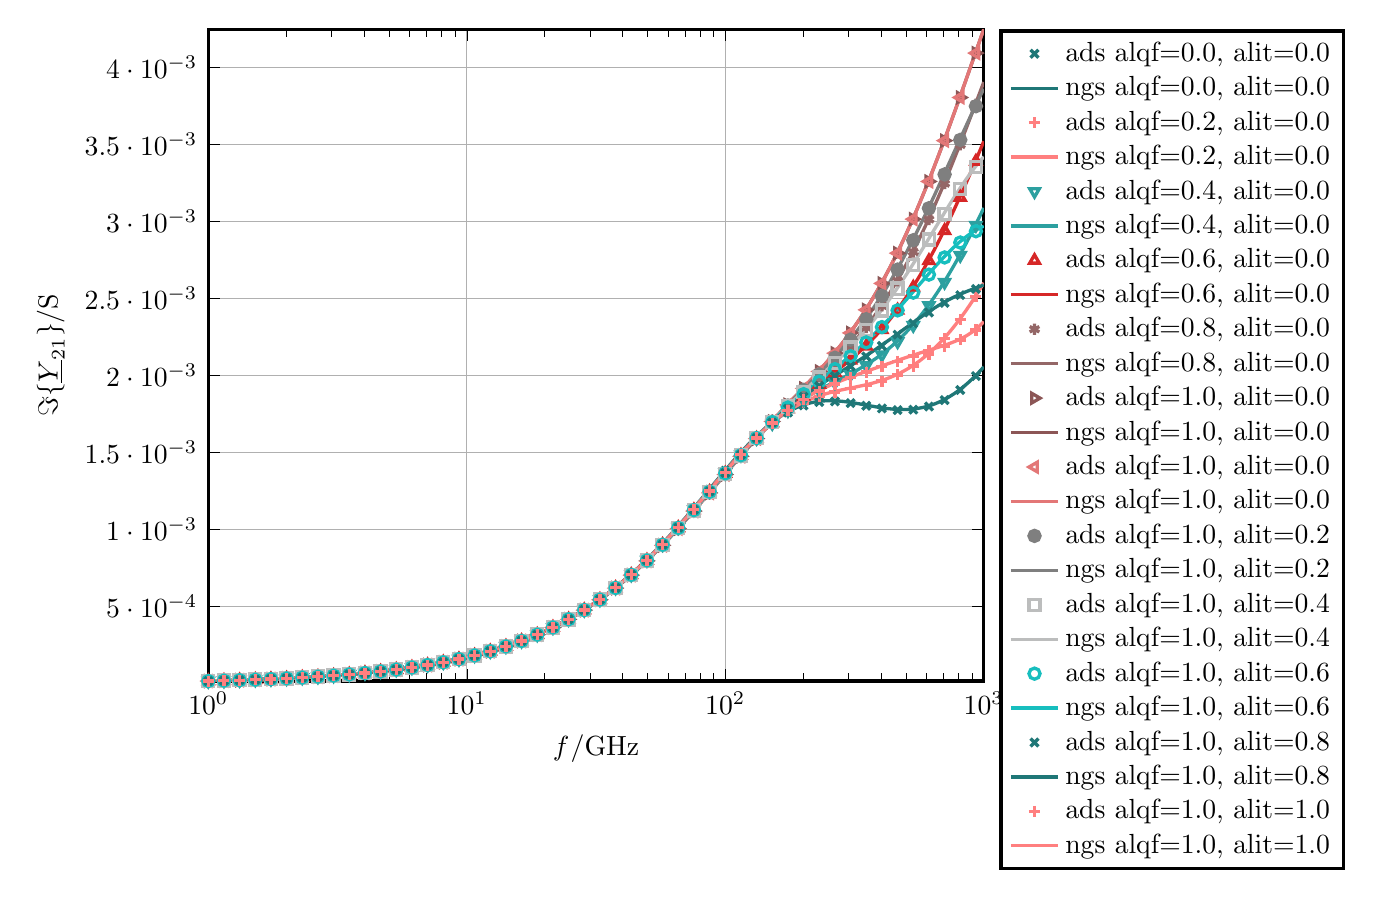
\begin{tikzpicture}[font=\normalsize]
\pgfplotsset{every axis/.append style={very thick}},
\definecolor{color0}{rgb}{0.12157, 0.46667, 0.46667}
\definecolor{color1}{rgb}{1.00000, 0.49804, 0.49804}
\definecolor{color2}{rgb}{0.17255, 0.62745, 0.62745}
\definecolor{color3}{rgb}{0.83922, 0.15294, 0.15294}
\definecolor{color4}{rgb}{0.58039, 0.40392, 0.40392}
\definecolor{color5}{rgb}{0.54902, 0.33725, 0.33725}
\definecolor{color6}{rgb}{0.89020, 0.46667, 0.46667}
\definecolor{color7}{rgb}{0.49804, 0.49804, 0.49804}
\definecolor{color8}{rgb}{0.73725, 0.74118, 0.74118}
\definecolor{color9}{rgb}{0.09020, 0.74510, 0.74510}

\begin{axis}[
width=4.5in,
xlabel={$f_{\mathrm{}}^{}/\si{\giga\hertz}$},
ylabel={$\Im\{\underline{Y}_{\mathrm{21}}^{}\}/\si{\siemens}$},
xmode=log,
% xmin=0,
% xmax=0,
% restrict x to domain=0:1,
log basis x=10,
% ymin=0,
% ymax=0,
% restrict y to domain=0:1,
log basis y=10,
xmajorgrids,
enlargelimits=false,
scaled ticks=false,
ymajorgrids,
x tick style={color=black},
y tick style={color=black},
x grid style={white!69.01960784313725!black},
y grid style={white!69.01960784313725!black},
/tikz/mark repeat=2,
legend style={at={(1.02,1.00)}, anchor=north west,legend cell align=left, align=left},
]
\addplot [color=color0, only marks, mark=x, mark options={solid}, mark phase=0, ]
  table[row sep=crcr, x expr=\thisrowno{0}*1.000000e-09, y expr=\thisrowno{1}*1.000000e+00]{
1e+09 1.71469e-05\\
1.07227e+09 1.83861e-05\\
1.14976e+09 1.97148e-05\\
1.23285e+09 2.11396e-05\\
1.32194e+09 2.26674e-05\\
1.41747e+09 2.43056e-05\\
1.51991e+09 2.60622e-05\\
1.62975e+09 2.79457e-05\\
1.74753e+09 2.99653e-05\\
1.87382e+09 3.21309e-05\\
2.00923e+09 3.4453e-05\\
2.15443e+09 3.69429e-05\\
2.31013e+09 3.96127e-05\\
2.47708e+09 4.24754e-05\\
2.65609e+09 4.55449e-05\\
2.84804e+09 4.88361e-05\\
3.05386e+09 5.23649e-05\\
3.27455e+09 5.61486e-05\\
3.51119e+09 6.02053e-05\\
3.76494e+09 6.45548e-05\\
4.03702e+09 6.92181e-05\\
4.32876e+09 7.42176e-05\\
4.64159e+09 7.95775e-05\\
4.97702e+09 8.53236e-05\\
5.3367e+09 9.14834e-05\\
5.72237e+09 9.80864e-05\\
6.13591e+09 0.000105164\\
6.57933e+09 0.000112751\\
7.0548e+09 0.000120882\\
7.56463e+09 0.000129596\\
8.11131e+09 0.000138934\\
8.69749e+09 0.00014894\\
9.32603e+09 0.000159661\\
1e+10 0.000171146\\
1.07227e+10 0.000183449\\
1.14976e+10 0.000196624\\
1.23285e+10 0.000210732\\
1.32194e+10 0.000225836\\
1.41747e+10 0.000242002\\
1.51991e+10 0.0002593\\
1.62975e+10 0.000277804\\
1.74753e+10 0.00029759\\
1.87382e+10 0.000318739\\
2.00923e+10 0.000341334\\
2.15443e+10 0.000365461\\
2.31013e+10 0.000391207\\
2.47708e+10 0.000418663\\
2.65609e+10 0.000447917\\
2.84804e+10 0.000479058\\
3.05386e+10 0.000512172\\
3.27455e+10 0.000547342\\
3.51119e+10 0.000584641\\
3.76494e+10 0.000624136\\
4.03702e+10 0.000665878\\
4.32876e+10 0.000709903\\
4.64159e+10 0.000756224\\
4.97702e+10 0.000804827\\
5.3367e+10 0.000855666\\
5.72237e+10 0.000908653\\
6.13591e+10 0.000963657\\
6.57933e+10 0.00102049\\
7.0548e+10 0.00107891\\
7.56463e+10 0.0011386\\
8.11131e+10 0.00119919\\
8.69749e+10 0.00126022\\
9.32603e+10 0.00132117\\
1e+11 0.00138146\\
1.07227e+11 0.00144042\\
1.14976e+11 0.00149739\\
1.23285e+11 0.00155165\\
1.32194e+11 0.0016025\\
1.41747e+11 0.00164928\\
1.51991e+11 0.00169138\\
1.62975e+11 0.0017283\\
1.74753e+11 0.00175968\\
1.87382e+11 0.00178528\\
2.00923e+11 0.00180507\\
2.15443e+11 0.00181918\\
2.31013e+11 0.00182792\\
2.47708e+11 0.00183178\\
2.65609e+11 0.00183138\\
2.84804e+11 0.00182748\\
3.05386e+11 0.0018209\\
3.27455e+11 0.00181253\\
3.51119e+11 0.00180331\\
3.76494e+11 0.00179413\\
4.03702e+11 0.00178588\\
4.32876e+11 0.00177942\\
4.64159e+11 0.0017755\\
4.97702e+11 0.00177486\\
5.3367e+11 0.00177812\\
5.72237e+11 0.00178585\\
6.13591e+11 0.00179853\\
6.57933e+11 0.00181657\\
7.0548e+11 0.0018403\\
7.56463e+11 0.00186999\\
8.11131e+11 0.00190581\\
8.69749e+11 0.00194788\\
9.32603e+11 0.00199623\\
1e+12 0.00205079\\
};
\addlegendentry{ads alqf=0.0, alit=0.0}
\addplot [color=color0, solid,  mark phase=0, ]
  table[row sep=crcr, x expr=\thisrowno{0}*1.000000e-09, y expr=\thisrowno{1}*1.000000e+00]{
1e+09 1.71874e-05\\
1.02306e+09 1.75838e-05\\
1.04665e+09 1.79893e-05\\
1.07079e+09 1.84041e-05\\
1.09548e+09 1.88285e-05\\
1.12074e+09 1.92627e-05\\
1.14658e+09 1.97069e-05\\
1.17302e+09 2.01614e-05\\
1.20007e+09 2.06263e-05\\
1.22775e+09 2.11019e-05\\
1.25606e+09 2.15886e-05\\
1.28502e+09 2.20864e-05\\
1.31466e+09 2.25957e-05\\
1.34497e+09 2.31168e-05\\
1.37599e+09 2.36499e-05\\
1.40772e+09 2.41953e-05\\
1.44018e+09 2.47533e-05\\
1.47339e+09 2.53241e-05\\
1.50736e+09 2.59081e-05\\
1.54212e+09 2.65055e-05\\
1.57768e+09 2.71168e-05\\
1.61406e+09 2.77421e-05\\
1.65128e+09 2.83819e-05\\
1.68936e+09 2.90364e-05\\
1.72832e+09 2.9706e-05\\
1.76817e+09 3.0391e-05\\
1.80895e+09 3.10918e-05\\
1.85066e+09 3.18088e-05\\
1.89334e+09 3.25424e-05\\
1.937e+09 3.32928e-05\\
1.98166e+09 3.40606e-05\\
2.02736e+09 3.4846e-05\\
2.07411e+09 3.56496e-05\\
2.12194e+09 3.64717e-05\\
2.17087e+09 3.73127e-05\\
2.22093e+09 3.81731e-05\\
2.27214e+09 3.90534e-05\\
2.32454e+09 3.9954e-05\\
2.37814e+09 4.08753e-05\\
2.43298e+09 4.18179e-05\\
2.48908e+09 4.27822e-05\\
2.54648e+09 4.37687e-05\\
2.6052e+09 4.4778e-05\\
2.66528e+09 4.58105e-05\\
2.72674e+09 4.68668e-05\\
2.78962e+09 4.79475e-05\\
2.85394e+09 4.9053e-05\\
2.91976e+09 5.01841e-05\\
2.98708e+09 5.13412e-05\\
3.05597e+09 5.25249e-05\\
3.12644e+09 5.3736e-05\\
3.19853e+09 5.49749e-05\\
3.27229e+09 5.62424e-05\\
3.34775e+09 5.75391e-05\\
3.42494e+09 5.88656e-05\\
3.50392e+09 6.02227e-05\\
3.58472e+09 6.1611e-05\\
3.66738e+09 6.30313e-05\\
3.75195e+09 6.44843e-05\\
3.83847e+09 6.59708e-05\\
3.92699e+09 6.74914e-05\\
4.01754e+09 6.90471e-05\\
4.11019e+09 7.06385e-05\\
4.20496e+09 7.22666e-05\\
4.30193e+09 7.39321e-05\\
4.40113e+09 7.5636e-05\\
4.50262e+09 7.7379e-05\\
4.60645e+09 7.91621e-05\\
4.71267e+09 8.09862e-05\\
4.82135e+09 8.28522e-05\\
4.93253e+09 8.47612e-05\\
5.04627e+09 8.67139e-05\\
5.16263e+09 8.87116e-05\\
5.28168e+09 9.07551e-05\\
5.40348e+09 9.28456e-05\\
5.52808e+09 9.49841e-05\\
5.65556e+09 9.71717e-05\\
5.78597e+09 9.94094e-05\\
5.91939e+09 0.000101699\\
6.05589e+09 0.00010404\\
6.19554e+09 0.000106436\\
6.33841e+09 0.000108886\\
6.48457e+09 0.000111392\\
6.6341e+09 0.000113956\\
6.78708e+09 0.000116579\\
6.94359e+09 0.000119261\\
7.10371e+09 0.000122005\\
7.26752e+09 0.000124812\\
7.43511e+09 0.000127683\\
7.60656e+09 0.00013062\\
7.78196e+09 0.000133624\\
7.96141e+09 0.000136696\\
8.145e+09 0.000139839\\
8.33282e+09 0.000143053\\
8.52497e+09 0.000146341\\
8.72156e+09 0.000149704\\
8.92267e+09 0.000153143\\
9.12843e+09 0.000156661\\
9.33893e+09 0.000160259\\
9.55428e+09 0.000163938\\
9.7746e+09 0.000167702\\
1e+10 0.000171551\\
1.02306e+10 0.000175487\\
1.04665e+10 0.000179512\\
1.07079e+10 0.000183629\\
1.09548e+10 0.00018784\\
1.12074e+10 0.000192145\\
1.14658e+10 0.000196548\\
1.17302e+10 0.000201051\\
1.20007e+10 0.000205655\\
1.22775e+10 0.000210363\\
1.25606e+10 0.000215177\\
1.28502e+10 0.000220099\\
1.31466e+10 0.000225133\\
1.34497e+10 0.000230279\\
1.37599e+10 0.00023554\\
1.40772e+10 0.00024092\\
1.44018e+10 0.00024642\\
1.47339e+10 0.000252043\\
1.50736e+10 0.000257791\\
1.54212e+10 0.000263667\\
1.57768e+10 0.000269674\\
1.61406e+10 0.000275814\\
1.65128e+10 0.00028209\\
1.68936e+10 0.000288505\\
1.72832e+10 0.000295062\\
1.76817e+10 0.000301763\\
1.80895e+10 0.000308611\\
1.85066e+10 0.00031561\\
1.89334e+10 0.000322762\\
1.937e+10 0.000330069\\
1.98166e+10 0.000337536\\
2.02736e+10 0.000345165\\
2.07411e+10 0.000352959\\
2.12194e+10 0.000360921\\
2.17087e+10 0.000369054\\
2.22093e+10 0.000377362\\
2.27214e+10 0.000385847\\
2.32454e+10 0.000394513\\
2.37814e+10 0.000403362\\
2.43298e+10 0.000412398\\
2.48908e+10 0.000421624\\
2.54648e+10 0.000431044\\
2.6052e+10 0.000440659\\
2.66528e+10 0.000450474\\
2.72674e+10 0.000460492\\
2.78962e+10 0.000470714\\
2.85394e+10 0.000481146\\
2.91976e+10 0.000491788\\
2.98708e+10 0.000502646\\
3.05597e+10 0.00051372\\
3.12644e+10 0.000525014\\
3.19853e+10 0.000536531\\
3.27229e+10 0.000548274\\
3.34775e+10 0.000560244\\
3.42494e+10 0.000572445\\
3.50392e+10 0.000584879\\
3.58472e+10 0.000597547\\
3.66738e+10 0.000610452\\
3.75195e+10 0.000623596\\
3.83847e+10 0.00063698\\
3.92699e+10 0.000650606\\
4.01754e+10 0.000664476\\
4.11019e+10 0.000678589\\
4.20496e+10 0.000692948\\
4.30193e+10 0.000707552\\
4.40113e+10 0.000722402\\
4.50262e+10 0.000737498\\
4.60645e+10 0.000752839\\
4.71267e+10 0.000768425\\
4.82135e+10 0.000784255\\
4.93253e+10 0.000800327\\
5.04627e+10 0.00081664\\
5.16263e+10 0.00083319\\
5.28168e+10 0.000849976\\
5.40348e+10 0.000866994\\
5.52808e+10 0.000884239\\
5.65556e+10 0.000901709\\
5.78597e+10 0.000919398\\
5.91939e+10 0.0009373\\
6.05589e+10 0.000955409\\
6.19554e+10 0.000973719\\
6.33841e+10 0.000992222\\
6.48457e+10 0.00101091\\
6.6341e+10 0.00102977\\
6.78708e+10 0.0010488\\
6.94359e+10 0.00106799\\
7.10371e+10 0.00108732\\
7.26752e+10 0.00110679\\
7.43511e+10 0.00112637\\
7.60656e+10 0.00114607\\
7.78196e+10 0.00116585\\
7.96141e+10 0.00118572\\
8.145e+10 0.00120564\\
8.33282e+10 0.00122561\\
8.52497e+10 0.00124561\\
8.72156e+10 0.00126561\\
8.92267e+10 0.00128561\\
9.12843e+10 0.00130557\\
9.33893e+10 0.00132548\\
9.55428e+10 0.00134533\\
9.7746e+10 0.00136507\\
1e+11 0.0013847\\
1.02306e+11 0.00140419\\
1.04665e+11 0.00142351\\
1.07079e+11 0.00144265\\
1.09548e+11 0.00146158\\
1.12074e+11 0.00148026\\
1.14658e+11 0.00149869\\
1.17302e+11 0.00151683\\
1.20007e+11 0.00153466\\
1.22775e+11 0.00155215\\
1.25606e+11 0.00156928\\
1.28502e+11 0.00158603\\
1.31466e+11 0.00160237\\
1.34497e+11 0.00161827\\
1.37599e+11 0.00163373\\
1.40772e+11 0.00164871\\
1.44018e+11 0.00166319\\
1.47339e+11 0.00167716\\
1.50736e+11 0.0016906\\
1.54212e+11 0.00170348\\
1.57768e+11 0.0017158\\
1.61406e+11 0.00172755\\
1.65128e+11 0.0017387\\
1.68936e+11 0.00174926\\
1.72832e+11 0.0017592\\
1.76817e+11 0.00176853\\
1.80895e+11 0.00177723\\
1.85066e+11 0.00178532\\
1.89334e+11 0.00179277\\
1.937e+11 0.00179961\\
1.98166e+11 0.00180583\\
2.02736e+11 0.00181143\\
2.07411e+11 0.00181643\\
2.12194e+11 0.00182083\\
2.17087e+11 0.00182465\\
2.22093e+11 0.0018279\\
2.27214e+11 0.00183059\\
2.32454e+11 0.00183274\\
2.37814e+11 0.00183438\\
2.43298e+11 0.00183552\\
2.48908e+11 0.00183618\\
2.54648e+11 0.0018364\\
2.6052e+11 0.00183618\\
2.66528e+11 0.00183557\\
2.72674e+11 0.00183459\\
2.78962e+11 0.00183326\\
2.85394e+11 0.00183162\\
2.91976e+11 0.00182969\\
2.98708e+11 0.00182751\\
3.05597e+11 0.00182511\\
3.12644e+11 0.00182252\\
3.19853e+11 0.00181978\\
3.27229e+11 0.0018169\\
3.34775e+11 0.00181394\\
3.42494e+11 0.00181091\\
3.50392e+11 0.00180785\\
3.58472e+11 0.0018048\\
3.66738e+11 0.00180178\\
3.75195e+11 0.00179883\\
3.83847e+11 0.00179597\\
3.92699e+11 0.00179323\\
4.01754e+11 0.00179066\\
4.11019e+11 0.00178826\\
4.20496e+11 0.00178608\\
4.30193e+11 0.00178414\\
4.40113e+11 0.00178247\\
4.50262e+11 0.00178109\\
4.60645e+11 0.00178003\\
4.71267e+11 0.00177931\\
4.82135e+11 0.00177895\\
4.93253e+11 0.00177899\\
5.04627e+11 0.00177943\\
5.16263e+11 0.00178031\\
5.28168e+11 0.00178163\\
5.40348e+11 0.00178343\\
5.52808e+11 0.00178571\\
5.65556e+11 0.00178851\\
5.78597e+11 0.00179182\\
5.91939e+11 0.00179567\\
6.05589e+11 0.00180007\\
6.19554e+11 0.00180504\\
6.33841e+11 0.00181059\\
6.48457e+11 0.00181673\\
6.6341e+11 0.00182347\\
6.78708e+11 0.00183083\\
6.94359e+11 0.00183881\\
7.10371e+11 0.00184742\\
7.26752e+11 0.00185667\\
7.43511e+11 0.00186657\\
7.60656e+11 0.00187712\\
7.78196e+11 0.00188833\\
7.96141e+11 0.0019002\\
8.145e+11 0.00191274\\
8.33282e+11 0.00192595\\
8.52497e+11 0.00193983\\
8.72156e+11 0.00195438\\
8.92267e+11 0.0019696\\
9.12843e+11 0.00198549\\
9.33893e+11 0.00200205\\
9.55428e+11 0.00201928\\
9.7746e+11 0.00203717\\
1e+12 0.00205571\\
};
\addlegendentry{ngs alqf=0.0, alit=0.0}
\addplot [color=color1, only marks, mark=+, mark options={solid}, mark phase=0, ]
  table[row sep=crcr, x expr=\thisrowno{0}*1.000000e-09, y expr=\thisrowno{1}*1.000000e+00]{
1e+09 1.71469e-05\\
1.07227e+09 1.83861e-05\\
1.14976e+09 1.97148e-05\\
1.23285e+09 2.11396e-05\\
1.32194e+09 2.26674e-05\\
1.41747e+09 2.43055e-05\\
1.51991e+09 2.60621e-05\\
1.62975e+09 2.79456e-05\\
1.74753e+09 2.99652e-05\\
1.87382e+09 3.21308e-05\\
2.00923e+09 3.44529e-05\\
2.15443e+09 3.69427e-05\\
2.31013e+09 3.96125e-05\\
2.47708e+09 4.24751e-05\\
2.65609e+09 4.55446e-05\\
2.84804e+09 4.88357e-05\\
3.05386e+09 5.23644e-05\\
3.27455e+09 5.6148e-05\\
3.51119e+09 6.02046e-05\\
3.76494e+09 6.45539e-05\\
4.03702e+09 6.92169e-05\\
4.32876e+09 7.42162e-05\\
4.64159e+09 7.95758e-05\\
4.97702e+09 8.53214e-05\\
5.3367e+09 9.14807e-05\\
5.72237e+09 9.80832e-05\\
6.13591e+09 0.00010516\\
6.57933e+09 0.000112746\\
7.0548e+09 0.000120876\\
7.56463e+09 0.000129588\\
8.11131e+09 0.000138925\\
8.69749e+09 0.000148929\\
9.32603e+09 0.000159647\\
1e+10 0.000171129\\
1.07227e+10 0.000183428\\
1.14976e+10 0.000196598\\
1.23285e+10 0.000210701\\
1.32194e+10 0.000225797\\
1.41747e+10 0.000241954\\
1.51991e+10 0.000259241\\
1.62975e+10 0.000277731\\
1.74753e+10 0.000297501\\
1.87382e+10 0.000318629\\
2.00923e+10 0.000341199\\
2.15443e+10 0.000365296\\
2.31013e+10 0.000391005\\
2.47708e+10 0.000418416\\
2.65609e+10 0.000447615\\
2.84804e+10 0.000478689\\
3.05386e+10 0.000511723\\
3.27455e+10 0.000546795\\
3.51119e+10 0.000583978\\
3.76494e+10 0.000623333\\
4.03702e+10 0.000664908\\
4.32876e+10 0.000708736\\
4.64159e+10 0.000754823\\
4.97702e+10 0.000803154\\
5.3367e+10 0.000853676\\
5.72237e+10 0.0009063\\
6.13591e+10 0.000960892\\
6.57933e+10 0.00101727\\
7.0548e+10 0.00107518\\
7.56463e+10 0.00113434\\
8.11131e+10 0.00119437\\
8.69749e+10 0.00125485\\
9.32603e+10 0.00131529\\
1e+11 0.00137515\\
1.07227e+11 0.00143385\\
1.14976e+11 0.00149079\\
1.23285e+11 0.00154537\\
1.32194e+11 0.00159699\\
1.41747e+11 0.00164514\\
1.51991e+11 0.00168936\\
1.62975e+11 0.00172932\\
1.74753e+11 0.00176481\\
1.87382e+11 0.00179578\\
2.00923e+11 0.00182233\\
2.15443e+11 0.00184475\\
2.31013e+11 0.00186344\\
2.47708e+11 0.00187898\\
2.65609e+11 0.00189205\\
2.84804e+11 0.00190339\\
3.05386e+11 0.00191384\\
3.27455e+11 0.00192424\\
3.51119e+11 0.00193542\\
3.76494e+11 0.0019482\\
4.03702e+11 0.00196336\\
4.32876e+11 0.00198161\\
4.64159e+11 0.00200358\\
4.97702e+11 0.00202985\\
5.3367e+11 0.00206088\\
5.72237e+11 0.00209709\\
6.13591e+11 0.00213879\\
6.57933e+11 0.00218622\\
7.0548e+11 0.00223954\\
7.56463e+11 0.00229884\\
8.11131e+11 0.00236411\\
8.69749e+11 0.00243528\\
9.32603e+11 0.00251219\\
1e+12 0.0025946\\
};
\addlegendentry{ads alqf=0.2, alit=0.0}
\addplot [color=color1, solid,  mark phase=0, ]
  table[row sep=crcr, x expr=\thisrowno{0}*1.000000e-09, y expr=\thisrowno{1}*1.000000e+00]{
1e+09 1.71874e-05\\
1.02306e+09 1.75837e-05\\
1.04665e+09 1.79892e-05\\
1.07079e+09 1.84041e-05\\
1.09548e+09 1.88285e-05\\
1.12074e+09 1.92627e-05\\
1.14658e+09 1.97069e-05\\
1.17302e+09 2.01613e-05\\
1.20007e+09 2.06263e-05\\
1.22775e+09 2.11019e-05\\
1.25606e+09 2.15885e-05\\
1.28502e+09 2.20864e-05\\
1.31466e+09 2.25957e-05\\
1.34497e+09 2.31168e-05\\
1.37599e+09 2.36499e-05\\
1.40772e+09 2.41952e-05\\
1.44018e+09 2.47532e-05\\
1.47339e+09 2.5324e-05\\
1.50736e+09 2.5908e-05\\
1.54212e+09 2.65055e-05\\
1.57768e+09 2.71167e-05\\
1.61406e+09 2.7742e-05\\
1.65128e+09 2.83818e-05\\
1.68936e+09 2.90363e-05\\
1.72832e+09 2.97059e-05\\
1.76817e+09 3.03909e-05\\
1.80895e+09 3.10917e-05\\
1.85066e+09 3.18087e-05\\
1.89334e+09 3.25423e-05\\
1.937e+09 3.32927e-05\\
1.98166e+09 3.40604e-05\\
2.02736e+09 3.48459e-05\\
2.07411e+09 3.56494e-05\\
2.12194e+09 3.64715e-05\\
2.17087e+09 3.73125e-05\\
2.22093e+09 3.8173e-05\\
2.27214e+09 3.90532e-05\\
2.32454e+09 3.99538e-05\\
2.37814e+09 4.08751e-05\\
2.43298e+09 4.18176e-05\\
2.48908e+09 4.27819e-05\\
2.54648e+09 4.37684e-05\\
2.6052e+09 4.47776e-05\\
2.66528e+09 4.58101e-05\\
2.72674e+09 4.68664e-05\\
2.78962e+09 4.79471e-05\\
2.85394e+09 4.90526e-05\\
2.91976e+09 5.01836e-05\\
2.98708e+09 5.13407e-05\\
3.05597e+09 5.25244e-05\\
3.12644e+09 5.37354e-05\\
3.19853e+09 5.49743e-05\\
3.27229e+09 5.62418e-05\\
3.34775e+09 5.75384e-05\\
3.42494e+09 5.88649e-05\\
3.50392e+09 6.02219e-05\\
3.58472e+09 6.16102e-05\\
3.66738e+09 6.30305e-05\\
3.75195e+09 6.44834e-05\\
3.83847e+09 6.59698e-05\\
3.92699e+09 6.74904e-05\\
4.01754e+09 6.90459e-05\\
4.11019e+09 7.06373e-05\\
4.20496e+09 7.22653e-05\\
4.30193e+09 7.39308e-05\\
4.40113e+09 7.56345e-05\\
4.50262e+09 7.73774e-05\\
4.60645e+09 7.91604e-05\\
4.71267e+09 8.09844e-05\\
4.82135e+09 8.28503e-05\\
4.93253e+09 8.47591e-05\\
5.04627e+09 8.67117e-05\\
5.16263e+09 8.87092e-05\\
5.28168e+09 9.07526e-05\\
5.40348e+09 9.28429e-05\\
5.52808e+09 9.49812e-05\\
5.65556e+09 9.71686e-05\\
5.78597e+09 9.94061e-05\\
5.91939e+09 0.000101695\\
6.05589e+09 0.000104036\\
6.19554e+09 0.000106431\\
6.33841e+09 0.000108881\\
6.48457e+09 0.000111388\\
6.6341e+09 0.000113951\\
6.78708e+09 0.000116573\\
6.94359e+09 0.000119256\\
7.10371e+09 0.000121999\\
7.26752e+09 0.000124806\\
7.43511e+09 0.000127676\\
7.60656e+09 0.000130612\\
7.78196e+09 0.000133616\\
7.96141e+09 0.000136688\\
8.145e+09 0.00013983\\
8.33282e+09 0.000143043\\
8.52497e+09 0.00014633\\
8.72156e+09 0.000149692\\
8.92267e+09 0.000153131\\
9.12843e+09 0.000156648\\
9.33893e+09 0.000160245\\
9.55428e+09 0.000163923\\
9.7746e+09 0.000167686\\
1e+10 0.000171533\\
1.02306e+10 0.000175468\\
1.04665e+10 0.000179493\\
1.07079e+10 0.000183608\\
1.09548e+10 0.000187817\\
1.12074e+10 0.000192121\\
1.14658e+10 0.000196522\\
1.17302e+10 0.000201023\\
1.20007e+10 0.000205625\\
1.22775e+10 0.000210331\\
1.25606e+10 0.000215143\\
1.28502e+10 0.000220063\\
1.31466e+10 0.000225094\\
1.34497e+10 0.000230237\\
1.37599e+10 0.000235496\\
1.40772e+10 0.000240873\\
1.44018e+10 0.000246369\\
1.47339e+10 0.000251988\\
1.50736e+10 0.000257733\\
1.54212e+10 0.000263605\\
1.57768e+10 0.000269607\\
1.61406e+10 0.000275743\\
1.65128e+10 0.000282014\\
1.68936e+10 0.000288424\\
1.72832e+10 0.000294975\\
1.76817e+10 0.00030167\\
1.80895e+10 0.000308512\\
1.85066e+10 0.000315504\\
1.89334e+10 0.000322648\\
1.937e+10 0.000329948\\
1.98166e+10 0.000337406\\
2.02736e+10 0.000345026\\
2.07411e+10 0.000352811\\
2.12194e+10 0.000360763\\
2.17087e+10 0.000368885\\
2.22093e+10 0.000377181\\
2.27214e+10 0.000385654\\
2.32454e+10 0.000394306\\
2.37814e+10 0.000403142\\
2.43298e+10 0.000412163\\
2.48908e+10 0.000421373\\
2.54648e+10 0.000430776\\
2.6052e+10 0.000440373\\
2.66528e+10 0.000450169\\
2.72674e+10 0.000460165\\
2.78962e+10 0.000470366\\
2.85394e+10 0.000480774\\
2.91976e+10 0.000491392\\
2.98708e+10 0.000502223\\
3.05597e+10 0.000513269\\
3.12644e+10 0.000524533\\
3.19853e+10 0.000536019\\
3.27229e+10 0.000547728\\
3.34775e+10 0.000559662\\
3.42494e+10 0.000571825\\
3.50392e+10 0.000584218\\
3.58472e+10 0.000596844\\
3.66738e+10 0.000609703\\
3.75195e+10 0.000622799\\
3.83847e+10 0.000636132\\
3.92699e+10 0.000649704\\
4.01754e+10 0.000663517\\
4.11019e+10 0.00067757\\
4.20496e+10 0.000691865\\
4.30193e+10 0.000706401\\
4.40113e+10 0.00072118\\
4.50262e+10 0.000736201\\
4.60645e+10 0.000751463\\
4.71267e+10 0.000766966\\
4.82135e+10 0.000782709\\
4.93253e+10 0.000798689\\
5.04627e+10 0.000814904\\
5.16263e+10 0.000831353\\
5.28168e+10 0.000848033\\
5.40348e+10 0.000864939\\
5.52808e+10 0.000882069\\
5.65556e+10 0.000899417\\
5.78597e+10 0.000916979\\
5.91939e+10 0.000934749\\
6.05589e+10 0.000952721\\
6.19554e+10 0.000970889\\
6.33841e+10 0.000989245\\
6.48457e+10 0.00100778\\
6.6341e+10 0.00102649\\
6.78708e+10 0.00104536\\
6.94359e+10 0.00106438\\
7.10371e+10 0.00108354\\
7.26752e+10 0.00110283\\
7.43511e+10 0.00112224\\
7.60656e+10 0.00114175\\
7.78196e+10 0.00116136\\
7.96141e+10 0.00118104\\
8.145e+10 0.00120078\\
8.33282e+10 0.00122057\\
8.52497e+10 0.00124038\\
8.72156e+10 0.00126021\\
8.92267e+10 0.00128003\\
9.12843e+10 0.00129983\\
9.33893e+10 0.00131958\\
9.55428e+10 0.00133927\\
9.7746e+10 0.00135888\\
1e+11 0.00137839\\
1.02306e+11 0.00139777\\
1.04665e+11 0.00141701\\
1.07079e+11 0.00143608\\
1.09548e+11 0.00145496\\
1.12074e+11 0.00147364\\
1.14658e+11 0.00149208\\
1.17302e+11 0.00151028\\
1.20007e+11 0.0015282\\
1.22775e+11 0.00154583\\
1.25606e+11 0.00156315\\
1.28502e+11 0.00158014\\
1.31466e+11 0.00159677\\
1.34497e+11 0.00161304\\
1.37599e+11 0.00162892\\
1.40772e+11 0.0016444\\
1.44018e+11 0.00165947\\
1.47339e+11 0.0016741\\
1.50736e+11 0.00168829\\
1.54212e+11 0.00170203\\
1.57768e+11 0.0017153\\
1.61406e+11 0.0017281\\
1.65128e+11 0.00174043\\
1.68936e+11 0.00175227\\
1.72832e+11 0.00176363\\
1.76817e+11 0.00177451\\
1.80895e+11 0.0017849\\
1.85066e+11 0.00179481\\
1.89334e+11 0.00180424\\
1.937e+11 0.0018132\\
1.98166e+11 0.0018217\\
2.02736e+11 0.00182975\\
2.07411e+11 0.00183736\\
2.12194e+11 0.00184454\\
2.17087e+11 0.00185132\\
2.22093e+11 0.0018577\\
2.27214e+11 0.00186371\\
2.32454e+11 0.00186936\\
2.37814e+11 0.00187468\\
2.43298e+11 0.00187969\\
2.48908e+11 0.00188442\\
2.54648e+11 0.00188888\\
2.6052e+11 0.00189311\\
2.66528e+11 0.00189714\\
2.72674e+11 0.00190098\\
2.78962e+11 0.00190467\\
2.85394e+11 0.00190824\\
2.91976e+11 0.00191172\\
2.98708e+11 0.00191513\\
3.05597e+11 0.00191851\\
3.12644e+11 0.00192188\\
3.19853e+11 0.00192527\\
3.27229e+11 0.00192873\\
3.34775e+11 0.00193226\\
3.42494e+11 0.00193591\\
3.50392e+11 0.0019397\\
3.58472e+11 0.00194366\\
3.66738e+11 0.00194781\\
3.75195e+11 0.00195219\\
3.83847e+11 0.00195682\\
3.92699e+11 0.00196173\\
4.01754e+11 0.00196694\\
4.11019e+11 0.00197247\\
4.20496e+11 0.00197836\\
4.30193e+11 0.00198461\\
4.40113e+11 0.00199126\\
4.50262e+11 0.00199833\\
4.60645e+11 0.00200582\\
4.71267e+11 0.00201378\\
4.82135e+11 0.0020222\\
4.93253e+11 0.00203111\\
5.04627e+11 0.00204053\\
5.16263e+11 0.00205047\\
5.28168e+11 0.00206094\\
5.40348e+11 0.00207196\\
5.52808e+11 0.00208354\\
5.65556e+11 0.00209569\\
5.78597e+11 0.00210843\\
5.91939e+11 0.00212176\\
6.05589e+11 0.00213569\\
6.19554e+11 0.00215023\\
6.33841e+11 0.00216539\\
6.48457e+11 0.00218116\\
6.6341e+11 0.00219757\\
6.78708e+11 0.00221461\\
6.94359e+11 0.00223228\\
7.10371e+11 0.0022506\\
7.26752e+11 0.00226955\\
7.43511e+11 0.00228914\\
7.60656e+11 0.00230937\\
7.78196e+11 0.00233024\\
7.96141e+11 0.00235175\\
8.145e+11 0.0023739\\
8.33282e+11 0.00239667\\
8.52497e+11 0.00242007\\
8.72156e+11 0.0024441\\
8.92267e+11 0.00246873\\
9.12843e+11 0.00249397\\
9.33893e+11 0.00251981\\
9.55428e+11 0.00254624\\
9.7746e+11 0.00257324\\
1e+12 0.0026008\\
};
\addlegendentry{ngs alqf=0.2, alit=0.0}
\addplot [color=color2, only marks, mark=triangle, mark options={solid, rotate=180}, mark phase=0, ]
  table[row sep=crcr, x expr=\thisrowno{0}*1.000000e-09, y expr=\thisrowno{1}*1.000000e+00]{
1e+09 1.71468e-05\\
1.07227e+09 1.8386e-05\\
1.14976e+09 1.97148e-05\\
1.23285e+09 2.11396e-05\\
1.32194e+09 2.26673e-05\\
1.41747e+09 2.43055e-05\\
1.51991e+09 2.6062e-05\\
1.62975e+09 2.79455e-05\\
1.74753e+09 2.99651e-05\\
1.87382e+09 3.21307e-05\\
2.00923e+09 3.44527e-05\\
2.15443e+09 3.69426e-05\\
2.31013e+09 3.96123e-05\\
2.47708e+09 4.24749e-05\\
2.65609e+09 4.55442e-05\\
2.84804e+09 4.88353e-05\\
3.05386e+09 5.23639e-05\\
3.27455e+09 5.61474e-05\\
3.51119e+09 6.02038e-05\\
3.76494e+09 6.4553e-05\\
4.03702e+09 6.92158e-05\\
4.32876e+09 7.42148e-05\\
4.64159e+09 7.95741e-05\\
4.97702e+09 8.53193e-05\\
5.3367e+09 9.14781e-05\\
5.72237e+09 9.808e-05\\
6.13591e+09 0.000105156\\
6.57933e+09 0.000112741\\
7.0548e+09 0.00012087\\
7.56463e+09 0.000129581\\
8.11131e+09 0.000138916\\
8.69749e+09 0.000148918\\
9.32603e+09 0.000159633\\
1e+10 0.000171112\\
1.07227e+10 0.000183407\\
1.14976e+10 0.000196573\\
1.23285e+10 0.000210669\\
1.32194e+10 0.000225758\\
1.41747e+10 0.000241906\\
1.51991e+10 0.000259182\\
1.62975e+10 0.000277659\\
1.74753e+10 0.000297412\\
1.87382e+10 0.00031852\\
2.00923e+10 0.000341066\\
2.15443e+10 0.000365133\\
2.31013e+10 0.000390805\\
2.47708e+10 0.000418171\\
2.65609e+10 0.000447317\\
2.84804e+10 0.000478326\\
3.05386e+10 0.000511281\\
3.27455e+10 0.000546258\\
3.51119e+10 0.000583327\\
3.76494e+10 0.000622546\\
4.03702e+10 0.00066396\\
4.32876e+10 0.000707597\\
4.64159e+10 0.000753462\\
4.97702e+10 0.000801533\\
5.3367e+10 0.000851756\\
5.72237e+10 0.000904041\\
6.13591e+10 0.000958252\\
6.57933e+10 0.00101421\\
7.0548e+10 0.00107167\\
7.56463e+10 0.00113036\\
8.11131e+10 0.00118991\\
8.69749e+10 0.00124995\\
9.32603e+10 0.00131001\\
1e+11 0.0013696\\
1.07227e+11 0.00142823\\
1.14976e+11 0.00148536\\
1.23285e+11 0.00154049\\
1.32194e+11 0.00159316\\
1.41747e+11 0.00164297\\
1.51991e+11 0.00168961\\
1.62975e+11 0.00173288\\
1.74753e+11 0.00177273\\
1.87382e+11 0.00180924\\
2.00923e+11 0.00184265\\
2.15443e+11 0.00187333\\
2.31013e+11 0.00190178\\
2.47708e+11 0.00192862\\
2.65609e+11 0.00195455\\
2.84804e+11 0.00198033\\
3.05386e+11 0.00200672\\
3.27455e+11 0.00203453\\
3.51119e+11 0.00206451\\
3.76494e+11 0.00209737\\
4.03702e+11 0.00213378\\
4.32876e+11 0.00217433\\
4.64159e+11 0.00221951\\
4.97702e+11 0.00226975\\
5.3367e+11 0.00232538\\
5.72237e+11 0.00238664\\
6.13591e+11 0.00245367\\
6.57933e+11 0.00252656\\
7.0548e+11 0.00260526\\
7.56463e+11 0.00268968\\
8.11131e+11 0.00277963\\
8.69749e+11 0.00287482\\
9.32603e+11 0.00297488\\
1e+12 0.00307935\\
};
\addlegendentry{ads alqf=0.4, alit=0.0}
\addplot [color=color2, solid,  mark phase=0, ]
  table[row sep=crcr, x expr=\thisrowno{0}*1.000000e-09, y expr=\thisrowno{1}*1.000000e+00]{
1e+09 1.71874e-05\\
1.02306e+09 1.75837e-05\\
1.04665e+09 1.79892e-05\\
1.07079e+09 1.84041e-05\\
1.09548e+09 1.88285e-05\\
1.12074e+09 1.92626e-05\\
1.14658e+09 1.97069e-05\\
1.17302e+09 2.01613e-05\\
1.20007e+09 2.06262e-05\\
1.22775e+09 2.11019e-05\\
1.25606e+09 2.15885e-05\\
1.28502e+09 2.20863e-05\\
1.31466e+09 2.25957e-05\\
1.34497e+09 2.31167e-05\\
1.37599e+09 2.36498e-05\\
1.40772e+09 2.41952e-05\\
1.44018e+09 2.47531e-05\\
1.47339e+09 2.5324e-05\\
1.50736e+09 2.5908e-05\\
1.54212e+09 2.65054e-05\\
1.57768e+09 2.71166e-05\\
1.61406e+09 2.7742e-05\\
1.65128e+09 2.83817e-05\\
1.68936e+09 2.90362e-05\\
1.72832e+09 2.97058e-05\\
1.76817e+09 3.03908e-05\\
1.80895e+09 3.10916e-05\\
1.85066e+09 3.18086e-05\\
1.89334e+09 3.25421e-05\\
1.937e+09 3.32926e-05\\
1.98166e+09 3.40603e-05\\
2.02736e+09 3.48457e-05\\
2.07411e+09 3.56493e-05\\
2.12194e+09 3.64713e-05\\
2.17087e+09 3.73124e-05\\
2.22093e+09 3.81728e-05\\
2.27214e+09 3.9053e-05\\
2.32454e+09 3.99536e-05\\
2.37814e+09 4.08748e-05\\
2.43298e+09 4.18174e-05\\
2.48908e+09 4.27816e-05\\
2.54648e+09 4.37681e-05\\
2.6052e+09 4.47773e-05\\
2.66528e+09 4.58098e-05\\
2.72674e+09 4.68661e-05\\
2.78962e+09 4.79467e-05\\
2.85394e+09 4.90522e-05\\
2.91976e+09 5.01832e-05\\
2.98708e+09 5.13403e-05\\
3.05597e+09 5.2524e-05\\
3.12644e+09 5.37349e-05\\
3.19853e+09 5.49738e-05\\
3.27229e+09 5.62412e-05\\
3.34775e+09 5.75378e-05\\
3.42494e+09 5.88642e-05\\
3.50392e+09 6.02212e-05\\
3.58472e+09 6.16094e-05\\
3.66738e+09 6.30296e-05\\
3.75195e+09 6.44825e-05\\
3.83847e+09 6.59688e-05\\
3.92699e+09 6.74893e-05\\
4.01754e+09 6.90448e-05\\
4.11019e+09 7.06361e-05\\
4.20496e+09 7.2264e-05\\
4.30193e+09 7.39294e-05\\
4.40113e+09 7.5633e-05\\
4.50262e+09 7.73758e-05\\
4.60645e+09 7.91587e-05\\
4.71267e+09 8.09826e-05\\
4.82135e+09 8.28484e-05\\
4.93253e+09 8.4757e-05\\
5.04627e+09 8.67095e-05\\
5.16263e+09 8.87069e-05\\
5.28168e+09 9.07501e-05\\
5.40348e+09 9.28402e-05\\
5.52808e+09 9.49783e-05\\
5.65556e+09 9.71655e-05\\
5.78597e+09 9.94028e-05\\
5.91939e+09 0.000101691\\
6.05589e+09 0.000104033\\
6.19554e+09 0.000106427\\
6.33841e+09 0.000108877\\
6.48457e+09 0.000111383\\
6.6341e+09 0.000113946\\
6.78708e+09 0.000116568\\
6.94359e+09 0.00011925\\
7.10371e+09 0.000121993\\
7.26752e+09 0.000124799\\
7.43511e+09 0.000127669\\
7.60656e+09 0.000130605\\
7.78196e+09 0.000133608\\
7.96141e+09 0.000136679\\
8.145e+09 0.00013982\\
8.33282e+09 0.000143033\\
8.52497e+09 0.00014632\\
8.72156e+09 0.000149681\\
8.92267e+09 0.000153119\\
9.12843e+09 0.000156635\\
9.33893e+09 0.000160231\\
9.55428e+09 0.000163908\\
9.7746e+09 0.00016767\\
1e+10 0.000171516\\
1.02306e+10 0.00017545\\
1.04665e+10 0.000179473\\
1.07079e+10 0.000183588\\
1.09548e+10 0.000187795\\
1.12074e+10 0.000192097\\
1.14658e+10 0.000196497\\
1.17302e+10 0.000200996\\
1.20007e+10 0.000205596\\
1.22775e+10 0.0002103\\
1.25606e+10 0.00021511\\
1.28502e+10 0.000220027\\
1.31466e+10 0.000225056\\
1.34497e+10 0.000230196\\
1.37599e+10 0.000235452\\
1.40772e+10 0.000240826\\
1.44018e+10 0.000246319\\
1.47339e+10 0.000251935\\
1.50736e+10 0.000257675\\
1.54212e+10 0.000263543\\
1.57768e+10 0.000269542\\
1.61406e+10 0.000275673\\
1.65128e+10 0.000281939\\
1.68936e+10 0.000288344\\
1.72832e+10 0.000294889\\
1.76817e+10 0.000301578\\
1.80895e+10 0.000308414\\
1.85066e+10 0.000315399\\
1.89334e+10 0.000322536\\
1.937e+10 0.000329828\\
1.98166e+10 0.000337278\\
2.02736e+10 0.000344889\\
2.07411e+10 0.000352664\\
2.12194e+10 0.000360606\\
2.17087e+10 0.000368718\\
2.22093e+10 0.000377002\\
2.27214e+10 0.000385463\\
2.32454e+10 0.000394103\\
2.37814e+10 0.000402924\\
2.43298e+10 0.000411931\\
2.48908e+10 0.000421125\\
2.54648e+10 0.000430511\\
2.6052e+10 0.00044009\\
2.66528e+10 0.000449867\\
2.72674e+10 0.000459844\\
2.78962e+10 0.000470023\\
2.85394e+10 0.000480408\\
2.91976e+10 0.000491002\\
2.98708e+10 0.000501806\\
3.05597e+10 0.000512825\\
3.12644e+10 0.00052406\\
3.19853e+10 0.000535515\\
3.27229e+10 0.000547191\\
3.34775e+10 0.00055909\\
3.42494e+10 0.000571216\\
3.50392e+10 0.00058357\\
3.58472e+10 0.000596154\\
3.66738e+10 0.000608969\\
3.75195e+10 0.000622018\\
3.83847e+10 0.000635302\\
3.92699e+10 0.000648822\\
4.01754e+10 0.000662579\\
4.11019e+10 0.000676574\\
4.20496e+10 0.000690808\\
4.30193e+10 0.00070528\\
4.40113e+10 0.00071999\\
4.50262e+10 0.000734939\\
4.60645e+10 0.000750126\\
4.71267e+10 0.000765549\\
4.82135e+10 0.000781208\\
4.93253e+10 0.000797101\\
5.04627e+10 0.000813225\\
5.16263e+10 0.000829578\\
5.28168e+10 0.000846157\\
5.40348e+10 0.000862959\\
5.52808e+10 0.00087998\\
5.65556e+10 0.000897214\\
5.78597e+10 0.000914658\\
5.91939e+10 0.000932306\\
6.05589e+10 0.000950152\\
6.19554e+10 0.000968189\\
6.33841e+10 0.000986409\\
6.48457e+10 0.00100481\\
6.6341e+10 0.00102337\\
6.78708e+10 0.00104209\\
6.94359e+10 0.00106097\\
7.10371e+10 0.00107998\\
7.26752e+10 0.00109911\\
7.43511e+10 0.00111837\\
7.60656e+10 0.00113773\\
7.78196e+10 0.00115717\\
7.96141e+10 0.0011767\\
8.145e+10 0.00119629\\
8.33282e+10 0.00121593\\
8.52497e+10 0.0012356\\
8.72156e+10 0.00125528\\
8.92267e+10 0.00127497\\
9.12843e+10 0.00129465\\
9.33893e+10 0.00131429\\
9.55428e+10 0.00133388\\
9.7746e+10 0.0013534\\
1e+11 0.00137284\\
1.02306e+11 0.00139217\\
1.04665e+11 0.00141138\\
1.07079e+11 0.00143045\\
1.09548e+11 0.00144936\\
1.12074e+11 0.0014681\\
1.14658e+11 0.00148664\\
1.17302e+11 0.00150496\\
1.20007e+11 0.00152306\\
1.22775e+11 0.00154091\\
1.25606e+11 0.00155851\\
1.28502e+11 0.00157582\\
1.31466e+11 0.00159285\\
1.34497e+11 0.00160957\\
1.37599e+11 0.00162597\\
1.40772e+11 0.00164205\\
1.44018e+11 0.00165779\\
1.47339e+11 0.00167318\\
1.50736e+11 0.00168822\\
1.54212e+11 0.0017029\\
1.57768e+11 0.00171722\\
1.61406e+11 0.00173117\\
1.65128e+11 0.00174476\\
1.68936e+11 0.00175797\\
1.72832e+11 0.00177083\\
1.76817e+11 0.00178332\\
1.80895e+11 0.00179546\\
1.85066e+11 0.00180725\\
1.89334e+11 0.0018187\\
1.937e+11 0.00182982\\
1.98166e+11 0.00184062\\
2.02736e+11 0.00185113\\
2.07411e+11 0.00186135\\
2.12194e+11 0.00187129\\
2.17087e+11 0.00188099\\
2.22093e+11 0.00189045\\
2.27214e+11 0.00189971\\
2.32454e+11 0.00190877\\
2.37814e+11 0.00191766\\
2.43298e+11 0.00192642\\
2.48908e+11 0.00193505\\
2.54648e+11 0.0019436\\
2.6052e+11 0.00195207\\
2.66528e+11 0.00196051\\
2.72674e+11 0.00196893\\
2.78962e+11 0.00197737\\
2.85394e+11 0.00198585\\
2.91976e+11 0.0019944\\
2.98708e+11 0.00200305\\
3.05597e+11 0.00201182\\
3.12644e+11 0.00202074\\
3.19853e+11 0.00202984\\
3.27229e+11 0.00203915\\
3.34775e+11 0.00204869\\
3.42494e+11 0.00205848\\
3.50392e+11 0.00206856\\
3.58472e+11 0.00207895\\
3.66738e+11 0.00208967\\
3.75195e+11 0.00210074\\
3.83847e+11 0.00211219\\
3.92699e+11 0.00212404\\
4.01754e+11 0.0021363\\
4.11019e+11 0.00214901\\
4.20496e+11 0.00216217\\
4.30193e+11 0.00217581\\
4.40113e+11 0.00218994\\
4.50262e+11 0.00220458\\
4.60645e+11 0.00221974\\
4.71267e+11 0.00223544\\
4.82135e+11 0.00225169\\
4.93253e+11 0.0022685\\
5.04627e+11 0.00228589\\
5.16263e+11 0.00230386\\
5.28168e+11 0.00232242\\
5.40348e+11 0.00234158\\
5.52808e+11 0.00236134\\
5.65556e+11 0.00238172\\
5.78597e+11 0.00240271\\
5.91939e+11 0.00242433\\
6.05589e+11 0.00244657\\
6.19554e+11 0.00246943\\
6.33841e+11 0.00249292\\
6.48457e+11 0.00251704\\
6.6341e+11 0.00254178\\
6.78708e+11 0.00256714\\
6.94359e+11 0.00259313\\
7.10371e+11 0.00261972\\
7.26752e+11 0.00264693\\
7.43511e+11 0.00267474\\
7.60656e+11 0.00270315\\
7.78196e+11 0.00273215\\
7.96141e+11 0.00276173\\
8.145e+11 0.00279188\\
8.33282e+11 0.00282258\\
8.52497e+11 0.00285384\\
8.72156e+11 0.00288563\\
8.92267e+11 0.00291793\\
9.12843e+11 0.00295074\\
9.33893e+11 0.00298404\\
9.55428e+11 0.00301781\\
9.7746e+11 0.00305203\\
1e+12 0.00308668\\
};
\addlegendentry{ngs alqf=0.4, alit=0.0}
\addplot [color=color3, only marks, mark=triangle, mark options={solid, rotate=0}, mark phase=0, ]
  table[row sep=crcr, x expr=\thisrowno{0}*1.000000e-09, y expr=\thisrowno{1}*1.000000e+00]{
1e+09 1.71468e-05\\
1.07227e+09 1.8386e-05\\
1.14976e+09 1.97148e-05\\
1.23285e+09 2.11395e-05\\
1.32194e+09 2.26673e-05\\
1.41747e+09 2.43054e-05\\
1.51991e+09 2.6062e-05\\
1.62975e+09 2.79455e-05\\
1.74753e+09 2.99651e-05\\
1.87382e+09 3.21306e-05\\
2.00923e+09 3.44526e-05\\
2.15443e+09 3.69424e-05\\
2.31013e+09 3.96121e-05\\
2.47708e+09 4.24746e-05\\
2.65609e+09 4.55439e-05\\
2.84804e+09 4.88349e-05\\
3.05386e+09 5.23635e-05\\
3.27455e+09 5.61468e-05\\
3.51119e+09 6.02031e-05\\
3.76494e+09 6.45521e-05\\
4.03702e+09 6.92147e-05\\
4.32876e+09 7.42134e-05\\
4.64159e+09 7.95724e-05\\
4.97702e+09 8.53172e-05\\
5.3367e+09 9.14756e-05\\
5.72237e+09 9.80768e-05\\
6.13591e+09 0.000105152\\
6.57933e+09 0.000112736\\
7.0548e+09 0.000120864\\
7.56463e+09 0.000129574\\
8.11131e+09 0.000138907\\
8.69749e+09 0.000148907\\
9.32603e+09 0.00015962\\
1e+10 0.000171095\\
1.07227e+10 0.000183386\\
1.14976e+10 0.000196547\\
1.23285e+10 0.000210637\\
1.32194e+10 0.00022572\\
1.41747e+10 0.000241859\\
1.51991e+10 0.000259124\\
1.62975e+10 0.000277587\\
1.74753e+10 0.000297324\\
1.87382e+10 0.000318413\\
2.00923e+10 0.000340934\\
2.15443e+10 0.000364971\\
2.31013e+10 0.000390608\\
2.47708e+10 0.00041793\\
2.65609e+10 0.000447023\\
2.84804e+10 0.000477968\\
3.05386e+10 0.000510846\\
3.27455e+10 0.000545731\\
3.51119e+10 0.000582689\\
3.76494e+10 0.000621776\\
4.03702e+10 0.000663035\\
4.32876e+10 0.000706489\\
4.64159e+10 0.000752141\\
4.97702e+10 0.000799966\\
5.3367e+10 0.000849908\\
5.72237e+10 0.000901876\\
6.13591e+10 0.000955736\\
6.57933e+10 0.00101131\\
7.0548e+10 0.00106838\\
7.56463e+10 0.00112665\\
8.11131e+10 0.00118582\\
8.69749e+10 0.00124551\\
9.32603e+10 0.00130531\\
1e+11 0.00136479\\
1.07227e+11 0.00142351\\
1.14976e+11 0.00148103\\
1.23285e+11 0.00153694\\
1.32194e+11 0.00159088\\
1.41747e+11 0.00164259\\
1.51991e+11 0.00169186\\
1.62975e+11 0.00173865\\
1.74753e+11 0.00178302\\
1.87382e+11 0.00182515\\
2.00923e+11 0.0018654\\
2.15443e+11 0.0019042\\
2.31013e+11 0.00194212\\
2.47708e+11 0.00197979\\
2.65609e+11 0.00201793\\
2.84804e+11 0.00205725\\
3.05386e+11 0.0020985\\
3.27455e+11 0.0021424\\
3.51119e+11 0.00218962\\
3.76494e+11 0.00224078\\
4.03702e+11 0.00229644\\
4.32876e+11 0.00235705\\
4.64159e+11 0.00242301\\
4.97702e+11 0.00249457\\
5.3367e+11 0.00257194\\
5.72237e+11 0.00265518\\
6.13591e+11 0.00274429\\
6.57933e+11 0.00283916\\
7.0548e+11 0.00293957\\
7.56463e+11 0.00304522\\
8.11131e+11 0.00315571\\
8.69749e+11 0.00327054\\
9.32603e+11 0.00338911\\
1e+12 0.00351071\\
};
\addlegendentry{ads alqf=0.6, alit=0.0}
\addplot [color=color3, solid,  mark phase=0, ]
  table[row sep=crcr, x expr=\thisrowno{0}*1.000000e-09, y expr=\thisrowno{1}*1.000000e+00]{
1e+09 1.71874e-05\\
1.02306e+09 1.75837e-05\\
1.04665e+09 1.79892e-05\\
1.07079e+09 1.8404e-05\\
1.09548e+09 1.88284e-05\\
1.12074e+09 1.92626e-05\\
1.14658e+09 1.97068e-05\\
1.17302e+09 2.01613e-05\\
1.20007e+09 2.06262e-05\\
1.22775e+09 2.11018e-05\\
1.25606e+09 2.15885e-05\\
1.28502e+09 2.20863e-05\\
1.31466e+09 2.25956e-05\\
1.34497e+09 2.31167e-05\\
1.37599e+09 2.36498e-05\\
1.40772e+09 2.41951e-05\\
1.44018e+09 2.47531e-05\\
1.47339e+09 2.53239e-05\\
1.50736e+09 2.59079e-05\\
1.54212e+09 2.65053e-05\\
1.57768e+09 2.71166e-05\\
1.61406e+09 2.77419e-05\\
1.65128e+09 2.83816e-05\\
1.68936e+09 2.90361e-05\\
1.72832e+09 2.97057e-05\\
1.76817e+09 3.03907e-05\\
1.80895e+09 3.10915e-05\\
1.85066e+09 3.18085e-05\\
1.89334e+09 3.2542e-05\\
1.937e+09 3.32924e-05\\
1.98166e+09 3.40602e-05\\
2.02736e+09 3.48456e-05\\
2.07411e+09 3.56491e-05\\
2.12194e+09 3.64712e-05\\
2.17087e+09 3.73122e-05\\
2.22093e+09 3.81726e-05\\
2.27214e+09 3.90528e-05\\
2.32454e+09 3.99533e-05\\
2.37814e+09 4.08746e-05\\
2.43298e+09 4.18171e-05\\
2.48908e+09 4.27814e-05\\
2.54648e+09 4.37678e-05\\
2.6052e+09 4.4777e-05\\
2.66528e+09 4.58095e-05\\
2.72674e+09 4.68657e-05\\
2.78962e+09 4.79463e-05\\
2.85394e+09 4.90518e-05\\
2.91976e+09 5.01828e-05\\
2.98708e+09 5.13398e-05\\
3.05597e+09 5.25235e-05\\
3.12644e+09 5.37344e-05\\
3.19853e+09 5.49732e-05\\
3.27229e+09 5.62406e-05\\
3.34775e+09 5.75371e-05\\
3.42494e+09 5.88635e-05\\
3.50392e+09 6.02205e-05\\
3.58472e+09 6.16086e-05\\
3.66738e+09 6.30288e-05\\
3.75195e+09 6.44816e-05\\
3.83847e+09 6.59678e-05\\
3.92699e+09 6.74883e-05\\
4.01754e+09 6.90437e-05\\
4.11019e+09 7.0635e-05\\
4.20496e+09 7.22628e-05\\
4.30193e+09 7.3928e-05\\
4.40113e+09 7.56316e-05\\
4.50262e+09 7.73743e-05\\
4.60645e+09 7.91571e-05\\
4.71267e+09 8.09808e-05\\
4.82135e+09 8.28465e-05\\
4.93253e+09 8.4755e-05\\
5.04627e+09 8.67073e-05\\
5.16263e+09 8.87045e-05\\
5.28168e+09 9.07476e-05\\
5.40348e+09 9.28375e-05\\
5.52808e+09 9.49754e-05\\
5.65556e+09 9.71624e-05\\
5.78597e+09 9.93995e-05\\
5.91939e+09 0.000101688\\
6.05589e+09 0.000104029\\
6.19554e+09 0.000106423\\
6.33841e+09 0.000108873\\
6.48457e+09 0.000111378\\
6.6341e+09 0.000113941\\
6.78708e+09 0.000116563\\
6.94359e+09 0.000119244\\
7.10371e+09 0.000121987\\
7.26752e+09 0.000124792\\
7.43511e+09 0.000127662\\
7.60656e+09 0.000130597\\
7.78196e+09 0.0001336\\
7.96141e+09 0.00013667\\
8.145e+09 0.000139811\\
8.33282e+09 0.000143024\\
8.52497e+09 0.000146309\\
8.72156e+09 0.00014967\\
8.92267e+09 0.000153107\\
9.12843e+09 0.000156622\\
9.33893e+09 0.000160217\\
9.55428e+09 0.000163894\\
9.7746e+09 0.000167654\\
1e+10 0.0001715\\
1.02306e+10 0.000175432\\
1.04665e+10 0.000179454\\
1.07079e+10 0.000183567\\
1.09548e+10 0.000187773\\
1.12074e+10 0.000192074\\
1.14658e+10 0.000196471\\
1.17302e+10 0.000200969\\
1.20007e+10 0.000205567\\
1.22775e+10 0.000210269\\
1.25606e+10 0.000215076\\
1.28502e+10 0.000219992\\
1.31466e+10 0.000225017\\
1.34497e+10 0.000230156\\
1.37599e+10 0.000235409\\
1.40772e+10 0.000240779\\
1.44018e+10 0.000246269\\
1.47339e+10 0.000251881\\
1.50736e+10 0.000257618\\
1.54212e+10 0.000263483\\
1.57768e+10 0.000269477\\
1.61406e+10 0.000275603\\
1.65128e+10 0.000281865\\
1.68936e+10 0.000288264\\
1.72832e+10 0.000294804\\
1.76817e+10 0.000301487\\
1.80895e+10 0.000308317\\
1.85066e+10 0.000315295\\
1.89334e+10 0.000322425\\
1.937e+10 0.000329709\\
1.98166e+10 0.000337151\\
2.02736e+10 0.000344754\\
2.07411e+10 0.000352519\\
2.12194e+10 0.000360451\\
2.17087e+10 0.000368552\\
2.22093e+10 0.000376826\\
2.27214e+10 0.000385274\\
2.32454e+10 0.000393901\\
2.37814e+10 0.000402709\\
2.43298e+10 0.000411701\\
2.48908e+10 0.00042088\\
2.54648e+10 0.000430249\\
2.6052e+10 0.000439812\\
2.66528e+10 0.00044957\\
2.72674e+10 0.000459526\\
2.78962e+10 0.000469685\\
2.85394e+10 0.000480047\\
2.91976e+10 0.000490617\\
2.98708e+10 0.000501397\\
3.05597e+10 0.000512389\\
3.12644e+10 0.000523595\\
3.19853e+10 0.000535019\\
3.27229e+10 0.000546663\\
3.34775e+10 0.000558529\\
3.42494e+10 0.000570619\\
3.50392e+10 0.000582934\\
3.58472e+10 0.000595478\\
3.66738e+10 0.000608251\\
3.75195e+10 0.000621255\\
3.83847e+10 0.000634491\\
3.92699e+10 0.00064796\\
4.01754e+10 0.000661664\\
4.11019e+10 0.000675603\\
4.20496e+10 0.000689777\\
4.30193e+10 0.000704187\\
4.40113e+10 0.000718832\\
4.50262e+10 0.000733713\\
4.60645e+10 0.000748827\\
4.71267e+10 0.000764175\\
4.82135e+10 0.000779755\\
4.93253e+10 0.000795565\\
5.04627e+10 0.000811602\\
5.16263e+10 0.000827865\\
5.28168e+10 0.00084435\\
5.40348e+10 0.000861054\\
5.52808e+10 0.000877973\\
5.65556e+10 0.000895102\\
5.78597e+10 0.000912437\\
5.91939e+10 0.000929972\\
6.05589e+10 0.000947701\\
6.19554e+10 0.000965618\\
6.33841e+10 0.000983716\\
6.48457e+10 0.00100199\\
6.6341e+10 0.00102042\\
6.78708e+10 0.00103902\\
6.94359e+10 0.00105776\\
7.10371e+10 0.00107663\\
7.26752e+10 0.00109564\\
7.43511e+10 0.00111476\\
7.60656e+10 0.00113398\\
7.78196e+10 0.0011533\\
7.96141e+10 0.0011727\\
8.145e+10 0.00119217\\
8.33282e+10 0.00121168\\
8.52497e+10 0.00123124\\
8.72156e+10 0.00125083\\
8.92267e+10 0.00127042\\
9.12843e+10 0.00129001\\
9.33893e+10 0.00130958\\
9.55428e+10 0.00132912\\
9.7746e+10 0.0013486\\
1e+11 0.00136802\\
1.02306e+11 0.00138736\\
1.04665e+11 0.0014066\\
1.07079e+11 0.00142572\\
1.09548e+11 0.00144472\\
1.12074e+11 0.00146358\\
1.14658e+11 0.00148228\\
1.17302e+11 0.00150081\\
1.20007e+11 0.00151915\\
1.22775e+11 0.0015373\\
1.25606e+11 0.00155524\\
1.28502e+11 0.00157296\\
1.31466e+11 0.00159045\\
1.34497e+11 0.0016077\\
1.37599e+11 0.00162471\\
1.40772e+11 0.00164146\\
1.44018e+11 0.00165795\\
1.47339e+11 0.00167418\\
1.50736e+11 0.00169014\\
1.54212e+11 0.00170584\\
1.57768e+11 0.00172127\\
1.61406e+11 0.00173643\\
1.65128e+11 0.00175134\\
1.68936e+11 0.00176598\\
1.72832e+11 0.00178037\\
1.76817e+11 0.00179452\\
1.80895e+11 0.00180844\\
1.85066e+11 0.00182213\\
1.89334e+11 0.00183561\\
1.937e+11 0.0018489\\
1.98166e+11 0.001862\\
2.02736e+11 0.00187494\\
2.07411e+11 0.00188772\\
2.12194e+11 0.00190038\\
2.17087e+11 0.00191293\\
2.22093e+11 0.0019254\\
2.27214e+11 0.00193779\\
2.32454e+11 0.00195015\\
2.37814e+11 0.00196248\\
2.43298e+11 0.00197482\\
2.48908e+11 0.00198718\\
2.54648e+11 0.0019996\\
2.6052e+11 0.00201211\\
2.66528e+11 0.00202471\\
2.72674e+11 0.00203745\\
2.78962e+11 0.00205034\\
2.85394e+11 0.00206342\\
2.91976e+11 0.00207671\\
2.98708e+11 0.00209023\\
3.05597e+11 0.00210401\\
3.12644e+11 0.00211807\\
3.19853e+11 0.00213244\\
3.27229e+11 0.00214715\\
3.34775e+11 0.00216221\\
3.42494e+11 0.00217765\\
3.50392e+11 0.00219348\\
3.58472e+11 0.00220974\\
3.66738e+11 0.00222644\\
3.75195e+11 0.0022436\\
3.83847e+11 0.00226124\\
3.92699e+11 0.00227937\\
4.01754e+11 0.00229802\\
4.11019e+11 0.0023172\\
4.20496e+11 0.00233692\\
4.30193e+11 0.00235719\\
4.40113e+11 0.00237803\\
4.50262e+11 0.00239945\\
4.60645e+11 0.00242147\\
4.71267e+11 0.00244408\\
4.82135e+11 0.00246729\\
4.93253e+11 0.00249112\\
5.04627e+11 0.00251557\\
5.16263e+11 0.00254065\\
5.28168e+11 0.00256634\\
5.40348e+11 0.00259267\\
5.52808e+11 0.00261963\\
5.65556e+11 0.00264722\\
5.78597e+11 0.00267544\\
5.91939e+11 0.00270428\\
6.05589e+11 0.00273375\\
6.19554e+11 0.00276384\\
6.33841e+11 0.00279454\\
6.48457e+11 0.00282585\\
6.6341e+11 0.00285776\\
6.78708e+11 0.00289025\\
6.94359e+11 0.00292333\\
7.10371e+11 0.00295697\\
7.26752e+11 0.00299118\\
7.43511e+11 0.00302592\\
7.60656e+11 0.0030612\\
7.78196e+11 0.00309699\\
7.96141e+11 0.00313328\\
8.145e+11 0.00317005\\
8.33282e+11 0.00320727\\
8.52497e+11 0.00324494\\
8.72156e+11 0.00328303\\
8.92267e+11 0.00332152\\
9.12843e+11 0.00336038\\
9.33893e+11 0.00339959\\
9.55428e+11 0.00343912\\
9.7746e+11 0.00347894\\
1e+12 0.00351903\\
};
\addlegendentry{ngs alqf=0.6, alit=0.0}
\addplot [color=color4, only marks, mark=asterisk, mark options={solid}, mark phase=0, ]
  table[row sep=crcr, x expr=\thisrowno{0}*1.000000e-09, y expr=\thisrowno{1}*1.000000e+00]{
1e+09 1.71468e-05\\
1.07227e+09 1.8386e-05\\
1.14976e+09 1.97147e-05\\
1.23285e+09 2.11395e-05\\
1.32194e+09 2.26672e-05\\
1.41747e+09 2.43054e-05\\
1.51991e+09 2.60619e-05\\
1.62975e+09 2.79454e-05\\
1.74753e+09 2.9965e-05\\
1.87382e+09 3.21305e-05\\
2.00923e+09 3.44525e-05\\
2.15443e+09 3.69422e-05\\
2.31013e+09 3.96119e-05\\
2.47708e+09 4.24744e-05\\
2.65609e+09 4.55436e-05\\
2.84804e+09 4.88345e-05\\
3.05386e+09 5.2363e-05\\
3.27455e+09 5.61462e-05\\
3.51119e+09 6.02024e-05\\
3.76494e+09 6.45512e-05\\
4.03702e+09 6.92136e-05\\
4.32876e+09 7.42121e-05\\
4.64159e+09 7.95707e-05\\
4.97702e+09 8.53152e-05\\
5.3367e+09 9.1473e-05\\
5.72237e+09 9.80736e-05\\
6.13591e+09 0.000105149\\
6.57933e+09 0.000112731\\
7.0548e+09 0.000120858\\
7.56463e+09 0.000129566\\
8.11131e+09 0.000138898\\
8.69749e+09 0.000148896\\
9.32603e+09 0.000159606\\
1e+10 0.000171079\\
1.07227e+10 0.000183365\\
1.14976e+10 0.000196522\\
1.23285e+10 0.000210606\\
1.32194e+10 0.000225681\\
1.41747e+10 0.000241812\\
1.51991e+10 0.000259066\\
1.62975e+10 0.000277516\\
1.74753e+10 0.000297237\\
1.87382e+10 0.000318306\\
2.00923e+10 0.000340804\\
2.15443e+10 0.000364811\\
2.31013e+10 0.000390413\\
2.47708e+10 0.000417692\\
2.65609e+10 0.000446733\\
2.84804e+10 0.000477615\\
3.05386e+10 0.000510418\\
3.27455e+10 0.000545213\\
3.51119e+10 0.000582064\\
3.76494e+10 0.000621024\\
4.03702e+10 0.000662133\\
4.32876e+10 0.000705412\\
4.64159e+10 0.00075086\\
4.97702e+10 0.000798452\\
5.3367e+10 0.000848131\\
5.72237e+10 0.000899806\\
6.13591e+10 0.000953346\\
6.57933e+10 0.00100858\\
7.0548e+10 0.00106529\\
7.56463e+10 0.00112322\\
8.11131e+10 0.00118208\\
8.69749e+10 0.00124151\\
9.32603e+10 0.00130117\\
1e+11 0.00136067\\
1.07227e+11 0.00141964\\
1.14976e+11 0.00147772\\
1.23285e+11 0.0015346\\
1.32194e+11 0.00159001\\
1.41747e+11 0.0016438\\
1.51991e+11 0.00169589\\
1.62975e+11 0.00174633\\
1.74753e+11 0.0017953\\
1.87382e+11 0.00184306\\
2.00923e+11 0.00189005\\
2.15443e+11 0.00193675\\
2.31013e+11 0.00198377\\
2.47708e+11 0.00203176\\
2.65609e+11 0.0020814\\
2.84804e+11 0.00213339\\
3.05386e+11 0.00218842\\
3.27455e+11 0.00224713\\
3.51119e+11 0.00231013\\
3.76494e+11 0.00237793\\
4.03702e+11 0.00245099\\
4.32876e+11 0.00252966\\
4.64159e+11 0.00261418\\
4.97702e+11 0.0027047\\
5.3367e+11 0.00280127\\
5.72237e+11 0.0029038\\
6.13591e+11 0.00301212\\
6.57933e+11 0.00312594\\
7.0548e+11 0.00324487\\
7.56463e+11 0.00336838\\
8.11131e+11 0.00349588\\
8.69749e+11 0.00362663\\
9.32603e+11 0.0037598\\
1e+12 0.00389443\\
};
\addlegendentry{ads alqf=0.8, alit=0.0}
\addplot [color=color4, solid,  mark phase=0, ]
  table[row sep=crcr, x expr=\thisrowno{0}*1.000000e-09, y expr=\thisrowno{1}*1.000000e+00]{
1e+09 1.71873e-05\\
1.02306e+09 1.75837e-05\\
1.04665e+09 1.79892e-05\\
1.07079e+09 1.8404e-05\\
1.09548e+09 1.88284e-05\\
1.12074e+09 1.92626e-05\\
1.14658e+09 1.97068e-05\\
1.17302e+09 2.01612e-05\\
1.20007e+09 2.06262e-05\\
1.22775e+09 2.11018e-05\\
1.25606e+09 2.15884e-05\\
1.28502e+09 2.20863e-05\\
1.31466e+09 2.25956e-05\\
1.34497e+09 2.31167e-05\\
1.37599e+09 2.36497e-05\\
1.40772e+09 2.41951e-05\\
1.44018e+09 2.4753e-05\\
1.47339e+09 2.53239e-05\\
1.50736e+09 2.59078e-05\\
1.54212e+09 2.65053e-05\\
1.57768e+09 2.71165e-05\\
1.61406e+09 2.77418e-05\\
1.65128e+09 2.83815e-05\\
1.68936e+09 2.9036e-05\\
1.72832e+09 2.97056e-05\\
1.76817e+09 3.03906e-05\\
1.80895e+09 3.10914e-05\\
1.85066e+09 3.18084e-05\\
1.89334e+09 3.25419e-05\\
1.937e+09 3.32923e-05\\
1.98166e+09 3.406e-05\\
2.02736e+09 3.48454e-05\\
2.07411e+09 3.5649e-05\\
2.12194e+09 3.6471e-05\\
2.17087e+09 3.7312e-05\\
2.22093e+09 3.81724e-05\\
2.27214e+09 3.90526e-05\\
2.32454e+09 3.99531e-05\\
2.37814e+09 4.08744e-05\\
2.43298e+09 4.18169e-05\\
2.48908e+09 4.27811e-05\\
2.54648e+09 4.37676e-05\\
2.6052e+09 4.47767e-05\\
2.66528e+09 4.58092e-05\\
2.72674e+09 4.68654e-05\\
2.78962e+09 4.7946e-05\\
2.85394e+09 4.90514e-05\\
2.91976e+09 5.01824e-05\\
2.98708e+09 5.13393e-05\\
3.05597e+09 5.2523e-05\\
3.12644e+09 5.37339e-05\\
3.19853e+09 5.49727e-05\\
3.27229e+09 5.624e-05\\
3.34775e+09 5.75365e-05\\
3.42494e+09 5.88628e-05\\
3.50392e+09 6.02197e-05\\
3.58472e+09 6.16079e-05\\
3.66738e+09 6.30279e-05\\
3.75195e+09 6.44807e-05\\
3.83847e+09 6.59669e-05\\
3.92699e+09 6.74873e-05\\
4.01754e+09 6.90426e-05\\
4.11019e+09 7.06338e-05\\
4.20496e+09 7.22615e-05\\
4.30193e+09 7.39267e-05\\
4.40113e+09 7.56301e-05\\
4.50262e+09 7.73727e-05\\
4.60645e+09 7.91554e-05\\
4.71267e+09 8.0979e-05\\
4.82135e+09 8.28446e-05\\
4.93253e+09 8.4753e-05\\
5.04627e+09 8.67052e-05\\
5.16263e+09 8.87022e-05\\
5.28168e+09 9.07451e-05\\
5.40348e+09 9.28348e-05\\
5.52808e+09 9.49726e-05\\
5.65556e+09 9.71593e-05\\
5.78597e+09 9.93962e-05\\
5.91939e+09 0.000101684\\
6.05589e+09 0.000104025\\
6.19554e+09 0.000106419\\
6.33841e+09 0.000108868\\
6.48457e+09 0.000111374\\
6.6341e+09 0.000113936\\
6.78708e+09 0.000116557\\
6.94359e+09 0.000119238\\
7.10371e+09 0.000121981\\
7.26752e+09 0.000124786\\
7.43511e+09 0.000127655\\
7.60656e+09 0.00013059\\
7.78196e+09 0.000133592\\
7.96141e+09 0.000136662\\
8.145e+09 0.000139802\\
8.33282e+09 0.000143014\\
8.52497e+09 0.000146299\\
8.72156e+09 0.000149659\\
8.92267e+09 0.000153095\\
9.12843e+09 0.000156609\\
9.33893e+09 0.000160203\\
9.55428e+09 0.000163879\\
9.7746e+09 0.000167638\\
1e+10 0.000171483\\
1.02306e+10 0.000175414\\
1.04665e+10 0.000179435\\
1.07079e+10 0.000183546\\
1.09548e+10 0.000187751\\
1.12074e+10 0.00019205\\
1.14658e+10 0.000196446\\
1.17302e+10 0.000200942\\
1.20007e+10 0.000205538\\
1.22775e+10 0.000210238\\
1.25606e+10 0.000215043\\
1.28502e+10 0.000219957\\
1.31466e+10 0.00022498\\
1.34497e+10 0.000230115\\
1.37599e+10 0.000235366\\
1.40772e+10 0.000240733\\
1.44018e+10 0.00024622\\
1.47339e+10 0.000251829\\
1.50736e+10 0.000257562\\
1.54212e+10 0.000263422\\
1.57768e+10 0.000269412\\
1.61406e+10 0.000275534\\
1.65128e+10 0.000281791\\
1.68936e+10 0.000288185\\
1.72832e+10 0.00029472\\
1.76817e+10 0.000301397\\
1.80895e+10 0.00030822\\
1.85066e+10 0.000315192\\
1.89334e+10 0.000322315\\
1.937e+10 0.000329592\\
1.98166e+10 0.000337026\\
2.02736e+10 0.000344619\\
2.07411e+10 0.000352376\\
2.12194e+10 0.000360298\\
2.17087e+10 0.000368389\\
2.22093e+10 0.000376651\\
2.27214e+10 0.000385088\\
2.32454e+10 0.000393702\\
2.37814e+10 0.000402497\\
2.43298e+10 0.000411475\\
2.48908e+10 0.000420639\\
2.54648e+10 0.000429992\\
2.6052e+10 0.000439537\\
2.66528e+10 0.000449276\\
2.72674e+10 0.000459214\\
2.78962e+10 0.000469351\\
2.85394e+10 0.000479692\\
2.91976e+10 0.000490239\\
2.98708e+10 0.000500994\\
3.05597e+10 0.000511959\\
3.12644e+10 0.000523138\\
3.19853e+10 0.000534533\\
3.27229e+10 0.000546146\\
3.34775e+10 0.000557978\\
3.42494e+10 0.000570033\\
3.50392e+10 0.000582312\\
3.58472e+10 0.000594816\\
3.66738e+10 0.000607547\\
3.75195e+10 0.000620508\\
3.83847e+10 0.000633698\\
3.92699e+10 0.000647119\\
4.01754e+10 0.000660772\\
4.11019e+10 0.000674657\\
4.20496e+10 0.000688774\\
4.30193e+10 0.000703125\\
4.40113e+10 0.000717707\\
4.50262e+10 0.000732522\\
4.60645e+10 0.000747568\\
4.71267e+10 0.000762844\\
4.82135e+10 0.000778349\\
4.93253e+10 0.000794081\\
5.04627e+10 0.000810037\\
5.16263e+10 0.000826215\\
5.28168e+10 0.000842612\\
5.40348e+10 0.000859224\\
5.52808e+10 0.000876048\\
5.65556e+10 0.00089308\\
5.78597e+10 0.000910314\\
5.91939e+10 0.000927746\\
6.05589e+10 0.000945369\\
6.19554e+10 0.000963178\\
6.33841e+10 0.000981165\\
6.48457e+10 0.000999324\\
6.6341e+10 0.00101765\\
6.78708e+10 0.00103612\\
6.94359e+10 0.00105475\\
7.10371e+10 0.00107351\\
7.26752e+10 0.0010924\\
7.43511e+10 0.00111141\\
7.60656e+10 0.00113053\\
7.78196e+10 0.00114974\\
7.96141e+10 0.00116903\\
8.145e+10 0.0011884\\
8.33282e+10 0.00120783\\
8.52497e+10 0.00122731\\
8.72156e+10 0.00124682\\
8.92267e+10 0.00126636\\
9.12843e+10 0.0012859\\
9.33893e+10 0.00130544\\
9.55428e+10 0.00132496\\
9.7746e+10 0.00134445\\
1e+11 0.0013639\\
1.02306e+11 0.00138329\\
1.04665e+11 0.00140261\\
1.07079e+11 0.00142185\\
1.09548e+11 0.00144099\\
1.12074e+11 0.00146003\\
1.14658e+11 0.00147895\\
1.17302e+11 0.00149774\\
1.20007e+11 0.00151639\\
1.22775e+11 0.0015349\\
1.25606e+11 0.00155325\\
1.28502e+11 0.00157144\\
1.31466e+11 0.00158945\\
1.34497e+11 0.0016073\\
1.37599e+11 0.00162497\\
1.40772e+11 0.00164246\\
1.44018e+11 0.00165976\\
1.47339e+11 0.00167688\\
1.50736e+11 0.00169382\\
1.54212e+11 0.00171059\\
1.57768e+11 0.00172718\\
1.61406e+11 0.00174359\\
1.65128e+11 0.00175985\\
1.68936e+11 0.00177595\\
1.72832e+11 0.00179191\\
1.76817e+11 0.00180773\\
1.80895e+11 0.00182343\\
1.85066e+11 0.00183902\\
1.89334e+11 0.00185452\\
1.937e+11 0.00186994\\
1.98166e+11 0.0018853\\
2.02736e+11 0.00190062\\
2.07411e+11 0.00191592\\
2.12194e+11 0.00193122\\
2.17087e+11 0.00194653\\
2.22093e+11 0.00196188\\
2.27214e+11 0.0019773\\
2.32454e+11 0.0019928\\
2.37814e+11 0.00200842\\
2.43298e+11 0.00202416\\
2.48908e+11 0.00204007\\
2.54648e+11 0.00205615\\
2.6052e+11 0.00207245\\
2.66528e+11 0.00208897\\
2.72674e+11 0.00210575\\
2.78962e+11 0.00212281\\
2.85394e+11 0.00214017\\
2.91976e+11 0.00215786\\
2.98708e+11 0.0021759\\
3.05597e+11 0.00219431\\
3.12644e+11 0.00221312\\
3.19853e+11 0.00223235\\
3.27229e+11 0.00225202\\
3.34775e+11 0.00227214\\
3.42494e+11 0.00229274\\
3.50392e+11 0.00231384\\
3.58472e+11 0.00233545\\
3.66738e+11 0.00235759\\
3.75195e+11 0.00238028\\
3.83847e+11 0.00240352\\
3.92699e+11 0.00242735\\
4.01754e+11 0.00245176\\
4.11019e+11 0.00247676\\
4.20496e+11 0.00250238\\
4.30193e+11 0.00252861\\
4.40113e+11 0.00255547\\
4.50262e+11 0.00258296\\
4.60645e+11 0.00261109\\
4.71267e+11 0.00263985\\
4.82135e+11 0.00266927\\
4.93253e+11 0.00269933\\
5.04627e+11 0.00273004\\
5.16263e+11 0.00276139\\
5.28168e+11 0.00279339\\
5.40348e+11 0.00282603\\
5.52808e+11 0.0028593\\
5.65556e+11 0.00289321\\
5.78597e+11 0.00292774\\
5.91939e+11 0.00296289\\
6.05589e+11 0.00299864\\
6.19554e+11 0.00303499\\
6.33841e+11 0.00307192\\
6.48457e+11 0.00310942\\
6.6341e+11 0.00314748\\
6.78708e+11 0.00318608\\
6.94359e+11 0.0032252\\
7.10371e+11 0.00326482\\
7.26752e+11 0.00330493\\
7.43511e+11 0.00334551\\
7.60656e+11 0.00338652\\
7.78196e+11 0.00342796\\
7.96141e+11 0.0034698\\
8.145e+11 0.003512\\
8.33282e+11 0.00355455\\
8.52497e+11 0.00359741\\
8.72156e+11 0.00364056\\
8.92267e+11 0.00368396\\
9.12843e+11 0.00372758\\
9.33893e+11 0.0037714\\
9.55428e+11 0.00381536\\
9.7746e+11 0.00385945\\
1e+12 0.00390361\\
};
\addlegendentry{ngs alqf=0.8, alit=0.0}
\addplot [color=color5, only marks, mark=triangle, mark options={solid, rotate=270}, mark phase=0, ]
  table[row sep=crcr, x expr=\thisrowno{0}*1.000000e-09, y expr=\thisrowno{1}*1.000000e+00]{
1e+09 1.71468e-05\\
1.07227e+09 1.8386e-05\\
1.14976e+09 1.97147e-05\\
1.23285e+09 2.11395e-05\\
1.32194e+09 2.26672e-05\\
1.41747e+09 2.43053e-05\\
1.51991e+09 2.60619e-05\\
1.62975e+09 2.79453e-05\\
1.74753e+09 2.99649e-05\\
1.87382e+09 3.21304e-05\\
2.00923e+09 3.44523e-05\\
2.15443e+09 3.69421e-05\\
2.31013e+09 3.96117e-05\\
2.47708e+09 4.24741e-05\\
2.65609e+09 4.55433e-05\\
2.84804e+09 4.88341e-05\\
3.05386e+09 5.23625e-05\\
3.27455e+09 5.61456e-05\\
3.51119e+09 6.02016e-05\\
3.76494e+09 6.45503e-05\\
4.03702e+09 6.92125e-05\\
4.32876e+09 7.42107e-05\\
4.64159e+09 7.9569e-05\\
4.97702e+09 8.53131e-05\\
5.3367e+09 9.14704e-05\\
5.72237e+09 9.80705e-05\\
6.13591e+09 0.000105145\\
6.57933e+09 0.000112727\\
7.0548e+09 0.000120852\\
7.56463e+09 0.000129559\\
8.11131e+09 0.000138889\\
8.69749e+09 0.000148885\\
9.32603e+09 0.000159593\\
1e+10 0.000171062\\
1.07227e+10 0.000183345\\
1.14976e+10 0.000196497\\
1.23285e+10 0.000210575\\
1.32194e+10 0.000225643\\
1.41747e+10 0.000241765\\
1.51991e+10 0.000259009\\
1.62975e+10 0.000277446\\
1.74753e+10 0.000297151\\
1.87382e+10 0.000318201\\
2.00923e+10 0.000340675\\
2.15443e+10 0.000364654\\
2.31013e+10 0.000390221\\
2.47708e+10 0.000417458\\
2.65609e+10 0.000446447\\
2.84804e+10 0.000477268\\
3.05386e+10 0.000509998\\
3.27455e+10 0.000544705\\
3.51119e+10 0.000581452\\
3.76494e+10 0.000620289\\
4.03702e+10 0.000661254\\
4.32876e+10 0.000704365\\
4.64159e+10 0.000749621\\
4.97702e+10 0.000796993\\
5.3367e+10 0.000846427\\
5.72237e+10 0.000897831\\
6.13591e+10 0.00095108\\
6.57933e+10 0.00100601\\
7.0548e+10 0.00106242\\
7.56463e+10 0.00112007\\
8.11131e+10 0.00117868\\
8.69749e+10 0.00123796\\
9.32603e+10 0.00129758\\
1e+11 0.00135722\\
1.07227e+11 0.00141658\\
1.14976e+11 0.00147537\\
1.23285e+11 0.00153337\\
1.32194e+11 0.00159042\\
1.41747e+11 0.00164644\\
1.51991e+11 0.00170147\\
1.62975e+11 0.00175564\\
1.74753e+11 0.00180922\\
1.87382e+11 0.00186256\\
2.00923e+11 0.00191613\\
2.15443e+11 0.00197047\\
2.31013e+11 0.00202619\\
2.47708e+11 0.00208393\\
2.65609e+11 0.00214437\\
2.84804e+11 0.00220816\\
3.05386e+11 0.00227593\\
3.27455e+11 0.00234826\\
3.51119e+11 0.00242567\\
3.76494e+11 0.0025086\\
4.03702e+11 0.00259739\\
4.32876e+11 0.00269228\\
4.64159e+11 0.0027934\\
4.97702e+11 0.00290078\\
5.3367e+11 0.00301431\\
5.72237e+11 0.00313376\\
6.13591e+11 0.00325881\\
6.57933e+11 0.00338897\\
7.0548e+11 0.00352365\\
7.56463e+11 0.00366216\\
8.11131e+11 0.00380366\\
8.69749e+11 0.00394721\\
9.32603e+11 0.00409172\\
1e+12 0.004236\\
};
\addlegendentry{ads alqf=1.0, alit=0.0}
\addplot [color=color5, solid,  mark phase=0, ]
  table[row sep=crcr, x expr=\thisrowno{0}*1.000000e-09, y expr=\thisrowno{1}*1.000000e+00]{
1e+09 1.71873e-05\\
1.02306e+09 1.75837e-05\\
1.04665e+09 1.79892e-05\\
1.07079e+09 1.8404e-05\\
1.09548e+09 1.88284e-05\\
1.12074e+09 1.92626e-05\\
1.14658e+09 1.97068e-05\\
1.17302e+09 2.01612e-05\\
1.20007e+09 2.06261e-05\\
1.22775e+09 2.11018e-05\\
1.25606e+09 2.15884e-05\\
1.28502e+09 2.20862e-05\\
1.31466e+09 2.25955e-05\\
1.34497e+09 2.31166e-05\\
1.37599e+09 2.36497e-05\\
1.40772e+09 2.41951e-05\\
1.44018e+09 2.4753e-05\\
1.47339e+09 2.53238e-05\\
1.50736e+09 2.59078e-05\\
1.54212e+09 2.65052e-05\\
1.57768e+09 2.71164e-05\\
1.61406e+09 2.77417e-05\\
1.65128e+09 2.83815e-05\\
1.68936e+09 2.9036e-05\\
1.72832e+09 2.97055e-05\\
1.76817e+09 3.03905e-05\\
1.80895e+09 3.10913e-05\\
1.85066e+09 3.18083e-05\\
1.89334e+09 3.25418e-05\\
1.937e+09 3.32922e-05\\
1.98166e+09 3.40599e-05\\
2.02736e+09 3.48453e-05\\
2.07411e+09 3.56488e-05\\
2.12194e+09 3.64709e-05\\
2.17087e+09 3.73118e-05\\
2.22093e+09 3.81722e-05\\
2.27214e+09 3.90524e-05\\
2.32454e+09 3.99529e-05\\
2.37814e+09 4.08742e-05\\
2.43298e+09 4.18166e-05\\
2.48908e+09 4.27809e-05\\
2.54648e+09 4.37673e-05\\
2.6052e+09 4.47764e-05\\
2.66528e+09 4.58089e-05\\
2.72674e+09 4.68651e-05\\
2.78962e+09 4.79456e-05\\
2.85394e+09 4.9051e-05\\
2.91976e+09 5.01819e-05\\
2.98708e+09 5.13389e-05\\
3.05597e+09 5.25225e-05\\
3.12644e+09 5.37334e-05\\
3.19853e+09 5.49721e-05\\
3.27229e+09 5.62394e-05\\
3.34775e+09 5.75359e-05\\
3.42494e+09 5.88622e-05\\
3.50392e+09 6.0219e-05\\
3.58472e+09 6.16071e-05\\
3.66738e+09 6.30271e-05\\
3.75195e+09 6.44798e-05\\
3.83847e+09 6.59659e-05\\
3.92699e+09 6.74862e-05\\
4.01754e+09 6.90415e-05\\
4.11019e+09 7.06326e-05\\
4.20496e+09 7.22603e-05\\
4.30193e+09 7.39253e-05\\
4.40113e+09 7.56287e-05\\
4.50262e+09 7.73712e-05\\
4.60645e+09 7.91538e-05\\
4.71267e+09 8.09773e-05\\
4.82135e+09 8.28427e-05\\
4.93253e+09 8.47509e-05\\
5.04627e+09 8.6703e-05\\
5.16263e+09 8.86999e-05\\
5.28168e+09 9.07426e-05\\
5.40348e+09 9.28322e-05\\
5.52808e+09 9.49697e-05\\
5.65556e+09 9.71563e-05\\
5.78597e+09 9.9393e-05\\
5.91939e+09 0.000101681\\
6.05589e+09 0.000104021\\
6.19554e+09 0.000106415\\
6.33841e+09 0.000108864\\
6.48457e+09 0.000111369\\
6.6341e+09 0.000113931\\
6.78708e+09 0.000116552\\
6.94359e+09 0.000119233\\
7.10371e+09 0.000121975\\
7.26752e+09 0.00012478\\
7.43511e+09 0.000127648\\
7.60656e+09 0.000130583\\
7.78196e+09 0.000133584\\
7.96141e+09 0.000136653\\
8.145e+09 0.000139793\\
8.33282e+09 0.000143004\\
8.52497e+09 0.000146289\\
8.72156e+09 0.000149648\\
8.92267e+09 0.000153083\\
9.12843e+09 0.000156596\\
9.33893e+09 0.00016019\\
9.55428e+09 0.000163865\\
9.7746e+09 0.000167623\\
1e+10 0.000171466\\
1.02306e+10 0.000175396\\
1.04665e+10 0.000179416\\
1.07079e+10 0.000183526\\
1.09548e+10 0.000187729\\
1.12074e+10 0.000192027\\
1.14658e+10 0.000196421\\
1.17302e+10 0.000200915\\
1.20007e+10 0.00020551\\
1.22775e+10 0.000210207\\
1.25606e+10 0.000215011\\
1.28502e+10 0.000219922\\
1.31466e+10 0.000224942\\
1.34497e+10 0.000230075\\
1.37599e+10 0.000235323\\
1.40772e+10 0.000240687\\
1.44018e+10 0.000246171\\
1.47339e+10 0.000251776\\
1.50736e+10 0.000257506\\
1.54212e+10 0.000263362\\
1.57768e+10 0.000269348\\
1.61406e+10 0.000275466\\
1.65128e+10 0.000281718\\
1.68936e+10 0.000288107\\
1.72832e+10 0.000294636\\
1.76817e+10 0.000301308\\
1.80895e+10 0.000308125\\
1.85066e+10 0.00031509\\
1.89334e+10 0.000322206\\
1.937e+10 0.000329475\\
1.98166e+10 0.000336901\\
2.02736e+10 0.000344487\\
2.07411e+10 0.000352234\\
2.12194e+10 0.000360147\\
2.17087e+10 0.000368228\\
2.22093e+10 0.000376479\\
2.27214e+10 0.000384904\\
2.32454e+10 0.000393506\\
2.37814e+10 0.000402287\\
2.43298e+10 0.000411251\\
2.48908e+10 0.0004204\\
2.54648e+10 0.000429738\\
2.6052e+10 0.000439266\\
2.66528e+10 0.000448988\\
2.72674e+10 0.000458906\\
2.78962e+10 0.000469023\\
2.85394e+10 0.000479343\\
2.91976e+10 0.000489867\\
2.98708e+10 0.000500597\\
3.05597e+10 0.000511538\\
3.12644e+10 0.000522689\\
3.19853e+10 0.000534055\\
3.27229e+10 0.000545638\\
3.34775e+10 0.000557438\\
3.42494e+10 0.000569459\\
3.50392e+10 0.000581702\\
3.58472e+10 0.000594168\\
3.66738e+10 0.00060686\\
3.75195e+10 0.000619778\\
3.83847e+10 0.000632924\\
3.92699e+10 0.000646298\\
4.01754e+10 0.000659902\\
4.11019e+10 0.000673735\\
4.20496e+10 0.000687799\\
4.30193e+10 0.000702092\\
4.40113e+10 0.000716616\\
4.50262e+10 0.000731368\\
4.60645e+10 0.000746349\\
4.71267e+10 0.000761558\\
4.82135e+10 0.000776992\\
4.93253e+10 0.000792649\\
5.04627e+10 0.000808529\\
5.16263e+10 0.000824628\\
5.28168e+10 0.000840943\\
5.40348e+10 0.000857471\\
5.52808e+10 0.000874208\\
5.65556e+10 0.00089115\\
5.78597e+10 0.000908292\\
5.91939e+10 0.000925629\\
6.05589e+10 0.000943156\\
6.19554e+10 0.000960868\\
6.33841e+10 0.000978756\\
6.48457e+10 0.000996816\\
6.6341e+10 0.00101504\\
6.78708e+10 0.00103342\\
6.94359e+10 0.00105194\\
7.10371e+10 0.00107061\\
7.26752e+10 0.0010894\\
7.43511e+10 0.00110832\\
7.60656e+10 0.00112735\\
7.78196e+10 0.00114647\\
7.96141e+10 0.00116569\\
8.145e+10 0.00118499\\
8.33282e+10 0.00120436\\
8.52497e+10 0.00122379\\
8.72156e+10 0.00124326\\
8.92267e+10 0.00126277\\
9.12843e+10 0.0012823\\
9.33893e+10 0.00130185\\
9.55428e+10 0.00132139\\
9.7746e+10 0.00134093\\
1e+11 0.00136045\\
1.02306e+11 0.00137994\\
1.04665e+11 0.00139938\\
1.07079e+11 0.00141878\\
1.09548e+11 0.00143811\\
1.12074e+11 0.00145738\\
1.14658e+11 0.00147657\\
1.17302e+11 0.00149567\\
1.20007e+11 0.00151468\\
1.22775e+11 0.0015336\\
1.25606e+11 0.00155241\\
1.28502e+11 0.00157112\\
1.31466e+11 0.00158972\\
1.34497e+11 0.00160821\\
1.37599e+11 0.00162659\\
1.40772e+11 0.00164486\\
1.44018e+11 0.00166303\\
1.47339e+11 0.00168108\\
1.50736e+11 0.00169904\\
1.54212e+11 0.0017169\\
1.57768e+11 0.00173468\\
1.61406e+11 0.00175237\\
1.65128e+11 0.00177\\
1.68936e+11 0.00178757\\
1.72832e+11 0.00180509\\
1.76817e+11 0.00182258\\
1.80895e+11 0.00184005\\
1.85066e+11 0.00185752\\
1.89334e+11 0.00187501\\
1.937e+11 0.00189252\\
1.98166e+11 0.00191008\\
2.02736e+11 0.00192772\\
2.07411e+11 0.00194544\\
2.12194e+11 0.00196328\\
2.17087e+11 0.00198125\\
2.22093e+11 0.00199937\\
2.27214e+11 0.00201767\\
2.32454e+11 0.00203617\\
2.37814e+11 0.0020549\\
2.43298e+11 0.00207387\\
2.48908e+11 0.00209311\\
2.54648e+11 0.00211264\\
2.6052e+11 0.00213249\\
2.66528e+11 0.00215268\\
2.72674e+11 0.00217323\\
2.78962e+11 0.00219417\\
2.85394e+11 0.00221551\\
2.91976e+11 0.00223729\\
2.98708e+11 0.00225951\\
3.05597e+11 0.0022822\\
3.12644e+11 0.00230538\\
3.19853e+11 0.00232907\\
3.27229e+11 0.00235328\\
3.34775e+11 0.00237804\\
3.42494e+11 0.00240336\\
3.50392e+11 0.00242925\\
3.58472e+11 0.00245574\\
3.66738e+11 0.00248282\\
3.75195e+11 0.00251053\\
3.83847e+11 0.00253885\\
3.92699e+11 0.00256782\\
4.01754e+11 0.00259743\\
4.11019e+11 0.00262769\\
4.20496e+11 0.0026586\\
4.30193e+11 0.00269019\\
4.40113e+11 0.00272244\\
4.50262e+11 0.00275535\\
4.60645e+11 0.00278894\\
4.71267e+11 0.0028232\\
4.82135e+11 0.00285813\\
4.93253e+11 0.00289372\\
5.04627e+11 0.00292998\\
5.16263e+11 0.00296688\\
5.28168e+11 0.00300444\\
5.40348e+11 0.00304264\\
5.52808e+11 0.00308146\\
5.65556e+11 0.0031209\\
5.78597e+11 0.00316095\\
5.91939e+11 0.00320159\\
6.05589e+11 0.0032428\\
6.19554e+11 0.00328458\\
6.33841e+11 0.00332689\\
6.48457e+11 0.00336972\\
6.6341e+11 0.00341305\\
6.78708e+11 0.00345686\\
6.94359e+11 0.00350112\\
7.10371e+11 0.0035458\\
7.26752e+11 0.00359089\\
7.43511e+11 0.00363635\\
7.60656e+11 0.00368215\\
7.78196e+11 0.00372826\\
7.96141e+11 0.00377466\\
8.145e+11 0.0038213\\
8.33282e+11 0.00386815\\
8.52497e+11 0.00391518\\
8.72156e+11 0.00396234\\
8.92267e+11 0.00400961\\
9.12843e+11 0.00405693\\
9.33893e+11 0.00410426\\
9.55428e+11 0.00415157\\
9.7746e+11 0.00419881\\
1e+12 0.00424592\\
};
\addlegendentry{ngs alqf=1.0, alit=0.0}
\addplot [color=color6, only marks, mark=triangle, mark options={solid, rotate=90}, mark phase=0, ]
  table[row sep=crcr, x expr=\thisrowno{0}*1.000000e-09, y expr=\thisrowno{1}*1.000000e+00]{
1e+09 1.71468e-05\\
1.07227e+09 1.8386e-05\\
1.14976e+09 1.97147e-05\\
1.23285e+09 2.11395e-05\\
1.32194e+09 2.26672e-05\\
1.41747e+09 2.43053e-05\\
1.51991e+09 2.60619e-05\\
1.62975e+09 2.79453e-05\\
1.74753e+09 2.99649e-05\\
1.87382e+09 3.21304e-05\\
2.00923e+09 3.44523e-05\\
2.15443e+09 3.69421e-05\\
2.31013e+09 3.96117e-05\\
2.47708e+09 4.24741e-05\\
2.65609e+09 4.55433e-05\\
2.84804e+09 4.88341e-05\\
3.05386e+09 5.23625e-05\\
3.27455e+09 5.61456e-05\\
3.51119e+09 6.02016e-05\\
3.76494e+09 6.45503e-05\\
4.03702e+09 6.92125e-05\\
4.32876e+09 7.42107e-05\\
4.64159e+09 7.9569e-05\\
4.97702e+09 8.53131e-05\\
5.3367e+09 9.14704e-05\\
5.72237e+09 9.80705e-05\\
6.13591e+09 0.000105145\\
6.57933e+09 0.000112727\\
7.0548e+09 0.000120852\\
7.56463e+09 0.000129559\\
8.11131e+09 0.000138889\\
8.69749e+09 0.000148885\\
9.32603e+09 0.000159593\\
1e+10 0.000171062\\
1.07227e+10 0.000183345\\
1.14976e+10 0.000196497\\
1.23285e+10 0.000210575\\
1.32194e+10 0.000225643\\
1.41747e+10 0.000241765\\
1.51991e+10 0.000259009\\
1.62975e+10 0.000277446\\
1.74753e+10 0.000297151\\
1.87382e+10 0.000318201\\
2.00923e+10 0.000340675\\
2.15443e+10 0.000364654\\
2.31013e+10 0.000390221\\
2.47708e+10 0.000417458\\
2.65609e+10 0.000446447\\
2.84804e+10 0.000477268\\
3.05386e+10 0.000509998\\
3.27455e+10 0.000544705\\
3.51119e+10 0.000581452\\
3.76494e+10 0.000620289\\
4.03702e+10 0.000661254\\
4.32876e+10 0.000704365\\
4.64159e+10 0.000749621\\
4.97702e+10 0.000796993\\
5.3367e+10 0.000846427\\
5.72237e+10 0.000897831\\
6.13591e+10 0.00095108\\
6.57933e+10 0.00100601\\
7.0548e+10 0.00106242\\
7.56463e+10 0.00112007\\
8.11131e+10 0.00117868\\
8.69749e+10 0.00123796\\
9.32603e+10 0.00129758\\
1e+11 0.00135722\\
1.07227e+11 0.00141658\\
1.14976e+11 0.00147537\\
1.23285e+11 0.00153337\\
1.32194e+11 0.00159042\\
1.41747e+11 0.00164644\\
1.51991e+11 0.00170147\\
1.62975e+11 0.00175564\\
1.74753e+11 0.00180922\\
1.87382e+11 0.00186256\\
2.00923e+11 0.00191613\\
2.15443e+11 0.00197047\\
2.31013e+11 0.00202619\\
2.47708e+11 0.00208393\\
2.65609e+11 0.00214437\\
2.84804e+11 0.00220816\\
3.05386e+11 0.00227593\\
3.27455e+11 0.00234826\\
3.51119e+11 0.00242567\\
3.76494e+11 0.0025086\\
4.03702e+11 0.00259739\\
4.32876e+11 0.00269228\\
4.64159e+11 0.0027934\\
4.97702e+11 0.00290078\\
5.3367e+11 0.00301431\\
5.72237e+11 0.00313376\\
6.13591e+11 0.00325881\\
6.57933e+11 0.00338897\\
7.0548e+11 0.00352365\\
7.56463e+11 0.00366216\\
8.11131e+11 0.00380366\\
8.69749e+11 0.00394721\\
9.32603e+11 0.00409172\\
1e+12 0.004236\\
};
\addlegendentry{ads alqf=1.0, alit=0.0}
\addplot [color=color6, solid,  mark phase=0, ]
  table[row sep=crcr, x expr=\thisrowno{0}*1.000000e-09, y expr=\thisrowno{1}*1.000000e+00]{
1e+09 1.71873e-05\\
1.02306e+09 1.75837e-05\\
1.04665e+09 1.79892e-05\\
1.07079e+09 1.8404e-05\\
1.09548e+09 1.88284e-05\\
1.12074e+09 1.92626e-05\\
1.14658e+09 1.97068e-05\\
1.17302e+09 2.01612e-05\\
1.20007e+09 2.06261e-05\\
1.22775e+09 2.11018e-05\\
1.25606e+09 2.15884e-05\\
1.28502e+09 2.20862e-05\\
1.31466e+09 2.25955e-05\\
1.34497e+09 2.31166e-05\\
1.37599e+09 2.36497e-05\\
1.40772e+09 2.41951e-05\\
1.44018e+09 2.4753e-05\\
1.47339e+09 2.53238e-05\\
1.50736e+09 2.59078e-05\\
1.54212e+09 2.65052e-05\\
1.57768e+09 2.71164e-05\\
1.61406e+09 2.77417e-05\\
1.65128e+09 2.83815e-05\\
1.68936e+09 2.9036e-05\\
1.72832e+09 2.97055e-05\\
1.76817e+09 3.03905e-05\\
1.80895e+09 3.10913e-05\\
1.85066e+09 3.18083e-05\\
1.89334e+09 3.25418e-05\\
1.937e+09 3.32922e-05\\
1.98166e+09 3.40599e-05\\
2.02736e+09 3.48453e-05\\
2.07411e+09 3.56488e-05\\
2.12194e+09 3.64709e-05\\
2.17087e+09 3.73118e-05\\
2.22093e+09 3.81722e-05\\
2.27214e+09 3.90524e-05\\
2.32454e+09 3.99529e-05\\
2.37814e+09 4.08742e-05\\
2.43298e+09 4.18166e-05\\
2.48908e+09 4.27809e-05\\
2.54648e+09 4.37673e-05\\
2.6052e+09 4.47764e-05\\
2.66528e+09 4.58089e-05\\
2.72674e+09 4.68651e-05\\
2.78962e+09 4.79456e-05\\
2.85394e+09 4.9051e-05\\
2.91976e+09 5.01819e-05\\
2.98708e+09 5.13389e-05\\
3.05597e+09 5.25225e-05\\
3.12644e+09 5.37334e-05\\
3.19853e+09 5.49721e-05\\
3.27229e+09 5.62394e-05\\
3.34775e+09 5.75359e-05\\
3.42494e+09 5.88622e-05\\
3.50392e+09 6.0219e-05\\
3.58472e+09 6.16071e-05\\
3.66738e+09 6.30271e-05\\
3.75195e+09 6.44798e-05\\
3.83847e+09 6.59659e-05\\
3.92699e+09 6.74862e-05\\
4.01754e+09 6.90415e-05\\
4.11019e+09 7.06326e-05\\
4.20496e+09 7.22603e-05\\
4.30193e+09 7.39253e-05\\
4.40113e+09 7.56287e-05\\
4.50262e+09 7.73712e-05\\
4.60645e+09 7.91538e-05\\
4.71267e+09 8.09773e-05\\
4.82135e+09 8.28427e-05\\
4.93253e+09 8.47509e-05\\
5.04627e+09 8.6703e-05\\
5.16263e+09 8.86999e-05\\
5.28168e+09 9.07426e-05\\
5.40348e+09 9.28322e-05\\
5.52808e+09 9.49697e-05\\
5.65556e+09 9.71563e-05\\
5.78597e+09 9.9393e-05\\
5.91939e+09 0.000101681\\
6.05589e+09 0.000104021\\
6.19554e+09 0.000106415\\
6.33841e+09 0.000108864\\
6.48457e+09 0.000111369\\
6.6341e+09 0.000113931\\
6.78708e+09 0.000116552\\
6.94359e+09 0.000119233\\
7.10371e+09 0.000121975\\
7.26752e+09 0.00012478\\
7.43511e+09 0.000127648\\
7.60656e+09 0.000130583\\
7.78196e+09 0.000133584\\
7.96141e+09 0.000136653\\
8.145e+09 0.000139793\\
8.33282e+09 0.000143004\\
8.52497e+09 0.000146289\\
8.72156e+09 0.000149648\\
8.92267e+09 0.000153083\\
9.12843e+09 0.000156596\\
9.33893e+09 0.00016019\\
9.55428e+09 0.000163865\\
9.7746e+09 0.000167623\\
1e+10 0.000171466\\
1.02306e+10 0.000175396\\
1.04665e+10 0.000179416\\
1.07079e+10 0.000183526\\
1.09548e+10 0.000187729\\
1.12074e+10 0.000192027\\
1.14658e+10 0.000196421\\
1.17302e+10 0.000200915\\
1.20007e+10 0.00020551\\
1.22775e+10 0.000210207\\
1.25606e+10 0.000215011\\
1.28502e+10 0.000219922\\
1.31466e+10 0.000224942\\
1.34497e+10 0.000230075\\
1.37599e+10 0.000235323\\
1.40772e+10 0.000240687\\
1.44018e+10 0.000246171\\
1.47339e+10 0.000251776\\
1.50736e+10 0.000257506\\
1.54212e+10 0.000263362\\
1.57768e+10 0.000269348\\
1.61406e+10 0.000275466\\
1.65128e+10 0.000281718\\
1.68936e+10 0.000288107\\
1.72832e+10 0.000294636\\
1.76817e+10 0.000301308\\
1.80895e+10 0.000308125\\
1.85066e+10 0.00031509\\
1.89334e+10 0.000322206\\
1.937e+10 0.000329475\\
1.98166e+10 0.000336901\\
2.02736e+10 0.000344487\\
2.07411e+10 0.000352234\\
2.12194e+10 0.000360147\\
2.17087e+10 0.000368228\\
2.22093e+10 0.000376479\\
2.27214e+10 0.000384904\\
2.32454e+10 0.000393506\\
2.37814e+10 0.000402287\\
2.43298e+10 0.000411251\\
2.48908e+10 0.0004204\\
2.54648e+10 0.000429738\\
2.6052e+10 0.000439266\\
2.66528e+10 0.000448988\\
2.72674e+10 0.000458906\\
2.78962e+10 0.000469023\\
2.85394e+10 0.000479343\\
2.91976e+10 0.000489867\\
2.98708e+10 0.000500597\\
3.05597e+10 0.000511538\\
3.12644e+10 0.000522689\\
3.19853e+10 0.000534055\\
3.27229e+10 0.000545638\\
3.34775e+10 0.000557438\\
3.42494e+10 0.000569459\\
3.50392e+10 0.000581702\\
3.58472e+10 0.000594168\\
3.66738e+10 0.00060686\\
3.75195e+10 0.000619778\\
3.83847e+10 0.000632924\\
3.92699e+10 0.000646298\\
4.01754e+10 0.000659902\\
4.11019e+10 0.000673735\\
4.20496e+10 0.000687799\\
4.30193e+10 0.000702092\\
4.40113e+10 0.000716616\\
4.50262e+10 0.000731368\\
4.60645e+10 0.000746349\\
4.71267e+10 0.000761558\\
4.82135e+10 0.000776992\\
4.93253e+10 0.000792649\\
5.04627e+10 0.000808529\\
5.16263e+10 0.000824628\\
5.28168e+10 0.000840943\\
5.40348e+10 0.000857471\\
5.52808e+10 0.000874208\\
5.65556e+10 0.00089115\\
5.78597e+10 0.000908292\\
5.91939e+10 0.000925629\\
6.05589e+10 0.000943156\\
6.19554e+10 0.000960868\\
6.33841e+10 0.000978756\\
6.48457e+10 0.000996816\\
6.6341e+10 0.00101504\\
6.78708e+10 0.00103342\\
6.94359e+10 0.00105194\\
7.10371e+10 0.00107061\\
7.26752e+10 0.0010894\\
7.43511e+10 0.00110832\\
7.60656e+10 0.00112735\\
7.78196e+10 0.00114647\\
7.96141e+10 0.00116569\\
8.145e+10 0.00118499\\
8.33282e+10 0.00120436\\
8.52497e+10 0.00122379\\
8.72156e+10 0.00124326\\
8.92267e+10 0.00126277\\
9.12843e+10 0.0012823\\
9.33893e+10 0.00130185\\
9.55428e+10 0.00132139\\
9.7746e+10 0.00134093\\
1e+11 0.00136045\\
1.02306e+11 0.00137994\\
1.04665e+11 0.00139938\\
1.07079e+11 0.00141878\\
1.09548e+11 0.00143811\\
1.12074e+11 0.00145738\\
1.14658e+11 0.00147657\\
1.17302e+11 0.00149567\\
1.20007e+11 0.00151468\\
1.22775e+11 0.0015336\\
1.25606e+11 0.00155241\\
1.28502e+11 0.00157112\\
1.31466e+11 0.00158972\\
1.34497e+11 0.00160821\\
1.37599e+11 0.00162659\\
1.40772e+11 0.00164486\\
1.44018e+11 0.00166303\\
1.47339e+11 0.00168108\\
1.50736e+11 0.00169904\\
1.54212e+11 0.0017169\\
1.57768e+11 0.00173468\\
1.61406e+11 0.00175237\\
1.65128e+11 0.00177\\
1.68936e+11 0.00178757\\
1.72832e+11 0.00180509\\
1.76817e+11 0.00182258\\
1.80895e+11 0.00184005\\
1.85066e+11 0.00185752\\
1.89334e+11 0.00187501\\
1.937e+11 0.00189252\\
1.98166e+11 0.00191008\\
2.02736e+11 0.00192772\\
2.07411e+11 0.00194544\\
2.12194e+11 0.00196328\\
2.17087e+11 0.00198125\\
2.22093e+11 0.00199937\\
2.27214e+11 0.00201767\\
2.32454e+11 0.00203617\\
2.37814e+11 0.0020549\\
2.43298e+11 0.00207387\\
2.48908e+11 0.00209311\\
2.54648e+11 0.00211264\\
2.6052e+11 0.00213249\\
2.66528e+11 0.00215268\\
2.72674e+11 0.00217323\\
2.78962e+11 0.00219417\\
2.85394e+11 0.00221551\\
2.91976e+11 0.00223729\\
2.98708e+11 0.00225951\\
3.05597e+11 0.0022822\\
3.12644e+11 0.00230538\\
3.19853e+11 0.00232907\\
3.27229e+11 0.00235328\\
3.34775e+11 0.00237804\\
3.42494e+11 0.00240336\\
3.50392e+11 0.00242925\\
3.58472e+11 0.00245574\\
3.66738e+11 0.00248282\\
3.75195e+11 0.00251053\\
3.83847e+11 0.00253885\\
3.92699e+11 0.00256782\\
4.01754e+11 0.00259743\\
4.11019e+11 0.00262769\\
4.20496e+11 0.0026586\\
4.30193e+11 0.00269019\\
4.40113e+11 0.00272244\\
4.50262e+11 0.00275535\\
4.60645e+11 0.00278894\\
4.71267e+11 0.0028232\\
4.82135e+11 0.00285813\\
4.93253e+11 0.00289372\\
5.04627e+11 0.00292998\\
5.16263e+11 0.00296688\\
5.28168e+11 0.00300444\\
5.40348e+11 0.00304264\\
5.52808e+11 0.00308146\\
5.65556e+11 0.0031209\\
5.78597e+11 0.00316095\\
5.91939e+11 0.00320159\\
6.05589e+11 0.0032428\\
6.19554e+11 0.00328458\\
6.33841e+11 0.00332689\\
6.48457e+11 0.00336972\\
6.6341e+11 0.00341305\\
6.78708e+11 0.00345686\\
6.94359e+11 0.00350112\\
7.10371e+11 0.0035458\\
7.26752e+11 0.00359089\\
7.43511e+11 0.00363635\\
7.60656e+11 0.00368215\\
7.78196e+11 0.00372826\\
7.96141e+11 0.00377466\\
8.145e+11 0.0038213\\
8.33282e+11 0.00386815\\
8.52497e+11 0.00391518\\
8.72156e+11 0.00396234\\
8.92267e+11 0.00400961\\
9.12843e+11 0.00405693\\
9.33893e+11 0.00410426\\
9.55428e+11 0.00415157\\
9.7746e+11 0.00419881\\
1e+12 0.00424592\\
};
\addlegendentry{ngs alqf=1.0, alit=0.0}
\addplot [color=color7, only marks, mark=*, mark options={solid, fill}, mark phase=0, ]
  table[row sep=crcr, x expr=\thisrowno{0}*1.000000e-09, y expr=\thisrowno{1}*1.000000e+00]{
1e+09 1.7146e-05\\
1.07227e+09 1.83851e-05\\
1.14976e+09 1.97138e-05\\
1.23285e+09 2.11384e-05\\
1.32194e+09 2.26661e-05\\
1.41747e+09 2.43042e-05\\
1.51991e+09 2.60606e-05\\
1.62975e+09 2.7944e-05\\
1.74753e+09 2.99635e-05\\
1.87382e+09 3.21289e-05\\
2.00923e+09 3.44507e-05\\
2.15443e+09 3.69403e-05\\
2.31013e+09 3.96098e-05\\
2.47708e+09 4.24722e-05\\
2.65609e+09 4.55412e-05\\
2.84804e+09 4.88319e-05\\
3.05386e+09 5.23602e-05\\
3.27455e+09 5.61432e-05\\
3.51119e+09 6.01991e-05\\
3.76494e+09 6.45476e-05\\
4.03702e+09 6.92097e-05\\
4.32876e+09 7.42079e-05\\
4.64159e+09 7.95661e-05\\
4.97702e+09 8.53101e-05\\
5.3367e+09 9.14675e-05\\
5.72237e+09 9.80676e-05\\
6.13591e+09 0.000105142\\
6.57933e+09 0.000112724\\
7.0548e+09 0.00012085\\
7.56463e+09 0.000129557\\
8.11131e+09 0.000138887\\
8.69749e+09 0.000148884\\
9.32603e+09 0.000159593\\
1e+10 0.000171064\\
1.07227e+10 0.000183348\\
1.14976e+10 0.000196502\\
1.23285e+10 0.000210584\\
1.32194e+10 0.000225655\\
1.41747e+10 0.000241782\\
1.51991e+10 0.000259031\\
1.62975e+10 0.000277476\\
1.74753e+10 0.000297189\\
1.87382e+10 0.00031825\\
2.00923e+10 0.000340737\\
2.15443e+10 0.000364733\\
2.31013e+10 0.00039032\\
2.47708e+10 0.000417582\\
2.65609e+10 0.000446602\\
2.84804e+10 0.00047746\\
3.05386e+10 0.000510233\\
3.27455e+10 0.000544993\\
3.51119e+10 0.000581804\\
3.76494e+10 0.000620717\\
4.03702e+10 0.000661771\\
4.32876e+10 0.000704988\\
4.64159e+10 0.000750366\\
4.97702e+10 0.00079788\\
5.3367e+10 0.000847473\\
5.72237e+10 0.000899057\\
6.13591e+10 0.000952505\\
6.57933e+10 0.00100765\\
7.0548e+10 0.00106428\\
7.56463e+10 0.00112216\\
8.11131e+10 0.00118099\\
8.69749e+10 0.00124045\\
9.32603e+10 0.00130022\\
1e+11 0.00135993\\
1.07227e+11 0.00141924\\
1.14976e+11 0.00147784\\
1.23285e+11 0.00153546\\
1.32194e+11 0.00159187\\
1.41747e+11 0.00164697\\
1.51991e+11 0.00170072\\
1.62975e+11 0.0017532\\
1.74753e+11 0.00180463\\
1.87382e+11 0.00185531\\
2.00923e+11 0.00190567\\
2.15443e+11 0.00195619\\
2.31013e+11 0.00200746\\
2.47708e+11 0.00206009\\
2.65609e+11 0.00211472\\
2.84804e+11 0.00217197\\
3.05386e+11 0.00223243\\
3.27455e+11 0.00229666\\
3.51119e+11 0.00236511\\
3.76494e+11 0.00243817\\
4.03702e+11 0.00251609\\
4.32876e+11 0.00259904\\
4.64159e+11 0.00268704\\
4.97702e+11 0.00277997\\
5.3367e+11 0.00287757\\
5.72237e+11 0.00297945\\
6.13591e+11 0.00308505\\
6.57933e+11 0.00319368\\
7.0548e+11 0.00330447\\
7.56463e+11 0.00341644\\
8.11131e+11 0.00352842\\
8.69749e+11 0.00363914\\
9.32603e+11 0.00374715\\
1e+12 0.00385086\\
};
\addlegendentry{ads alqf=1.0, alit=0.2}
\addplot [color=color7, solid,  mark phase=0, ]
  table[row sep=crcr, x expr=\thisrowno{0}*1.000000e-09, y expr=\thisrowno{1}*1.000000e+00]{
1e+09 1.71865e-05\\
1.02306e+09 1.75828e-05\\
1.04665e+09 1.79883e-05\\
1.07079e+09 1.84031e-05\\
1.09548e+09 1.88275e-05\\
1.12074e+09 1.92616e-05\\
1.14658e+09 1.97058e-05\\
1.17302e+09 2.01602e-05\\
1.20007e+09 2.06251e-05\\
1.22775e+09 2.11008e-05\\
1.25606e+09 2.15874e-05\\
1.28502e+09 2.20852e-05\\
1.31466e+09 2.25945e-05\\
1.34497e+09 2.31155e-05\\
1.37599e+09 2.36485e-05\\
1.40772e+09 2.41939e-05\\
1.44018e+09 2.47518e-05\\
1.47339e+09 2.53226e-05\\
1.50736e+09 2.59065e-05\\
1.54212e+09 2.65039e-05\\
1.57768e+09 2.71151e-05\\
1.61406e+09 2.77404e-05\\
1.65128e+09 2.83801e-05\\
1.68936e+09 2.90346e-05\\
1.72832e+09 2.97041e-05\\
1.76817e+09 3.03891e-05\\
1.80895e+09 3.10899e-05\\
1.85066e+09 3.18068e-05\\
1.89334e+09 3.25403e-05\\
1.937e+09 3.32906e-05\\
1.98166e+09 3.40583e-05\\
2.02736e+09 3.48437e-05\\
2.07411e+09 3.56471e-05\\
2.12194e+09 3.64691e-05\\
2.17087e+09 3.73101e-05\\
2.22093e+09 3.81704e-05\\
2.27214e+09 3.90506e-05\\
2.32454e+09 3.99511e-05\\
2.37814e+09 4.08723e-05\\
2.43298e+09 4.18147e-05\\
2.48908e+09 4.27789e-05\\
2.54648e+09 4.37653e-05\\
2.6052e+09 4.47744e-05\\
2.66528e+09 4.58068e-05\\
2.72674e+09 4.6863e-05\\
2.78962e+09 4.79435e-05\\
2.85394e+09 4.90489e-05\\
2.91976e+09 5.01797e-05\\
2.98708e+09 5.13366e-05\\
3.05597e+09 5.25202e-05\\
3.12644e+09 5.3731e-05\\
3.19853e+09 5.49697e-05\\
3.27229e+09 5.6237e-05\\
3.34775e+09 5.75334e-05\\
3.42494e+09 5.88597e-05\\
3.50392e+09 6.02165e-05\\
3.58472e+09 6.16045e-05\\
3.66738e+09 6.30245e-05\\
3.75195e+09 6.44772e-05\\
3.83847e+09 6.59632e-05\\
3.92699e+09 6.74835e-05\\
4.01754e+09 6.90388e-05\\
4.11019e+09 7.06298e-05\\
4.20496e+09 7.22575e-05\\
4.30193e+09 7.39225e-05\\
4.40113e+09 7.56258e-05\\
4.50262e+09 7.73683e-05\\
4.60645e+09 7.91509e-05\\
4.71267e+09 8.09744e-05\\
4.82135e+09 8.28397e-05\\
4.93253e+09 8.4748e-05\\
5.04627e+09 8.67e-05\\
5.16263e+09 8.86969e-05\\
5.28168e+09 9.07396e-05\\
5.40348e+09 9.28292e-05\\
5.52808e+09 9.49668e-05\\
5.65556e+09 9.71533e-05\\
5.78597e+09 9.939e-05\\
5.91939e+09 0.000101678\\
6.05589e+09 0.000104018\\
6.19554e+09 0.000106412\\
6.33841e+09 0.000108861\\
6.48457e+09 0.000111366\\
6.6341e+09 0.000113929\\
6.78708e+09 0.00011655\\
6.94359e+09 0.00011923\\
7.10371e+09 0.000121973\\
7.26752e+09 0.000124777\\
7.43511e+09 0.000127646\\
7.60656e+09 0.000130581\\
7.78196e+09 0.000133582\\
7.96141e+09 0.000136652\\
8.145e+09 0.000139792\\
8.33282e+09 0.000143003\\
8.52497e+09 0.000146288\\
8.72156e+09 0.000149647\\
8.92267e+09 0.000153083\\
9.12843e+09 0.000156596\\
9.33893e+09 0.00016019\\
9.55428e+09 0.000163865\\
9.7746e+09 0.000167624\\
1e+10 0.000171468\\
1.02306e+10 0.000175399\\
1.04665e+10 0.000179419\\
1.07079e+10 0.000183529\\
1.09548e+10 0.000187733\\
1.12074e+10 0.000192032\\
1.14658e+10 0.000196427\\
1.17302e+10 0.000200921\\
1.20007e+10 0.000205517\\
1.22775e+10 0.000210216\\
1.25606e+10 0.00021502\\
1.28502e+10 0.000219932\\
1.31466e+10 0.000224954\\
1.34497e+10 0.000230088\\
1.37599e+10 0.000235337\\
1.40772e+10 0.000240703\\
1.44018e+10 0.000246189\\
1.47339e+10 0.000251796\\
1.50736e+10 0.000257528\\
1.54212e+10 0.000263386\\
1.57768e+10 0.000269374\\
1.61406e+10 0.000275494\\
1.65128e+10 0.000281749\\
1.68936e+10 0.000288141\\
1.72832e+10 0.000294673\\
1.76817e+10 0.000301348\\
1.80895e+10 0.000308168\\
1.85066e+10 0.000315137\\
1.89334e+10 0.000322257\\
1.937e+10 0.000329531\\
1.98166e+10 0.000336961\\
2.02736e+10 0.000344551\\
2.07411e+10 0.000352304\\
2.12194e+10 0.000360222\\
2.17087e+10 0.000368309\\
2.22093e+10 0.000376567\\
2.27214e+10 0.000384999\\
2.32454e+10 0.000393608\\
2.37814e+10 0.000402397\\
2.43298e+10 0.000411369\\
2.48908e+10 0.000420527\\
2.54648e+10 0.000429873\\
2.6052e+10 0.000439411\\
2.66528e+10 0.000449144\\
2.72674e+10 0.000459073\\
2.78962e+10 0.000469203\\
2.85394e+10 0.000479535\\
2.91976e+10 0.000490073\\
2.98708e+10 0.000500818\\
3.05597e+10 0.000511774\\
3.12644e+10 0.000522942\\
3.19853e+10 0.000534325\\
3.27229e+10 0.000545926\\
3.34775e+10 0.000557746\\
3.42494e+10 0.000569788\\
3.50392e+10 0.000582052\\
3.58472e+10 0.000594542\\
3.66738e+10 0.000607258\\
3.75195e+10 0.000620203\\
3.83847e+10 0.000633376\\
3.92699e+10 0.000646779\\
4.01754e+10 0.000660413\\
4.11019e+10 0.000674279\\
4.20496e+10 0.000688377\\
4.30193e+10 0.000702706\\
4.40113e+10 0.000717267\\
4.50262e+10 0.000732059\\
4.60645e+10 0.000747081\\
4.71267e+10 0.000762333\\
4.82135e+10 0.000777812\\
4.93253e+10 0.000793518\\
5.04627e+10 0.000809447\\
5.16263e+10 0.000825597\\
5.28168e+10 0.000841966\\
5.40348e+10 0.000858549\\
5.52808e+10 0.000875344\\
5.65556e+10 0.000892346\\
5.78597e+10 0.00090955\\
5.91939e+10 0.000926952\\
6.05589e+10 0.000944545\\
6.19554e+10 0.000962323\\
6.33841e+10 0.000980281\\
6.48457e+10 0.000998411\\
6.6341e+10 0.00101671\\
6.78708e+10 0.00103516\\
6.94359e+10 0.00105376\\
7.10371e+10 0.0010725\\
7.26752e+10 0.00109137\\
7.43511e+10 0.00111036\\
7.60656e+10 0.00112946\\
7.78196e+10 0.00114866\\
7.96141e+10 0.00116794\\
8.145e+10 0.00118731\\
8.33282e+10 0.00120675\\
8.52497e+10 0.00122623\\
8.72156e+10 0.00124576\\
8.92267e+10 0.00126532\\
9.12843e+10 0.0012849\\
9.33893e+10 0.00130449\\
9.55428e+10 0.00132407\\
9.7746e+10 0.00134363\\
1e+11 0.00136316\\
1.02306e+11 0.00138264\\
1.04665e+11 0.00140208\\
1.07079e+11 0.00142144\\
1.09548e+11 0.00144074\\
1.12074e+11 0.00145994\\
1.14658e+11 0.00147905\\
1.17302e+11 0.00149805\\
1.20007e+11 0.00151694\\
1.22775e+11 0.00153571\\
1.25606e+11 0.00155436\\
1.28502e+11 0.00157286\\
1.31466e+11 0.00159124\\
1.34497e+11 0.00160946\\
1.37599e+11 0.00162755\\
1.40772e+11 0.00164549\\
1.44018e+11 0.00166329\\
1.47339e+11 0.00168094\\
1.50736e+11 0.00169845\\
1.54212e+11 0.00171582\\
1.57768e+11 0.00173306\\
1.61406e+11 0.00175018\\
1.65128e+11 0.00176718\\
1.68936e+11 0.00178406\\
1.72832e+11 0.00180086\\
1.76817e+11 0.00181756\\
1.80895e+11 0.00183419\\
1.85066e+11 0.00185076\\
1.89334e+11 0.00186728\\
1.937e+11 0.00188378\\
1.98166e+11 0.00190026\\
2.02736e+11 0.00191676\\
2.07411e+11 0.00193327\\
2.12194e+11 0.00194984\\
2.17087e+11 0.00196647\\
2.22093e+11 0.00198318\\
2.27214e+11 0.002\\
2.32454e+11 0.00201696\\
2.37814e+11 0.00203406\\
2.43298e+11 0.00205134\\
2.48908e+11 0.00206881\\
2.54648e+11 0.00208651\\
2.6052e+11 0.00210444\\
2.66528e+11 0.00212263\\
2.72674e+11 0.00214111\\
2.78962e+11 0.0021599\\
2.85394e+11 0.00217901\\
2.91976e+11 0.00219847\\
2.98708e+11 0.00221829\\
3.05597e+11 0.0022385\\
3.12644e+11 0.00225912\\
3.19853e+11 0.00228015\\
3.27229e+11 0.00230162\\
3.34775e+11 0.00232354\\
3.42494e+11 0.00234593\\
3.50392e+11 0.0023688\\
3.58472e+11 0.00239217\\
3.66738e+11 0.00241603\\
3.75195e+11 0.00244041\\
3.83847e+11 0.00246531\\
3.92699e+11 0.00249074\\
4.01754e+11 0.0025167\\
4.11019e+11 0.00254319\\
4.20496e+11 0.00257023\\
4.30193e+11 0.00259781\\
4.40113e+11 0.00262593\\
4.50262e+11 0.00265459\\
4.60645e+11 0.00268379\\
4.71267e+11 0.00271351\\
4.82135e+11 0.00274376\\
4.93253e+11 0.00277453\\
5.04627e+11 0.0028058\\
5.16263e+11 0.00283757\\
5.28168e+11 0.00286981\\
5.40348e+11 0.00290252\\
5.52808e+11 0.00293568\\
5.65556e+11 0.00296927\\
5.78597e+11 0.00300327\\
5.91939e+11 0.00303766\\
6.05589e+11 0.00307241\\
6.19554e+11 0.0031075\\
6.33841e+11 0.00314291\\
6.48457e+11 0.00317859\\
6.6341e+11 0.00321453\\
6.78708e+11 0.00325069\\
6.94359e+11 0.00328704\\
7.10371e+11 0.00332354\\
7.26752e+11 0.00336015\\
7.43511e+11 0.00339684\\
7.60656e+11 0.00343356\\
7.78196e+11 0.00347027\\
7.96141e+11 0.00350693\\
8.145e+11 0.00354349\\
8.33282e+11 0.00357991\\
8.52497e+11 0.00361613\\
8.72156e+11 0.00365211\\
8.92267e+11 0.0036878\\
9.12843e+11 0.00372313\\
9.33893e+11 0.00375806\\
9.55428e+11 0.00379252\\
9.7746e+11 0.00382646\\
1e+12 0.00385982\\
};
\addlegendentry{ngs alqf=1.0, alit=0.2}
\addplot [color=color8, only marks, mark=square, mark options={solid}, mark phase=0, ]
  table[row sep=crcr, x expr=\thisrowno{0}*1.000000e-09, y expr=\thisrowno{1}*1.000000e+00]{
1e+09 1.71451e-05\\
1.07227e+09 1.83842e-05\\
1.14976e+09 1.97128e-05\\
1.23285e+09 2.11374e-05\\
1.32194e+09 2.2665e-05\\
1.41747e+09 2.4303e-05\\
1.51991e+09 2.60594e-05\\
1.62975e+09 2.79426e-05\\
1.74753e+09 2.9962e-05\\
1.87382e+09 3.21273e-05\\
2.00923e+09 3.44491e-05\\
2.15443e+09 3.69386e-05\\
2.31013e+09 3.9608e-05\\
2.47708e+09 4.24702e-05\\
2.65609e+09 4.55392e-05\\
2.84804e+09 4.88298e-05\\
3.05386e+09 5.23579e-05\\
3.27455e+09 5.61408e-05\\
3.51119e+09 6.01966e-05\\
3.76494e+09 6.4545e-05\\
4.03702e+09 6.9207e-05\\
4.32876e+09 7.42051e-05\\
4.64159e+09 7.95632e-05\\
4.97702e+09 8.53072e-05\\
5.3367e+09 9.14645e-05\\
5.72237e+09 9.80647e-05\\
6.13591e+09 0.000105139\\
6.57933e+09 0.000112721\\
7.0548e+09 0.000120847\\
7.56463e+09 0.000129555\\
8.11131e+09 0.000138886\\
8.69749e+09 0.000148883\\
9.32603e+09 0.000159593\\
1e+10 0.000171066\\
1.07227e+10 0.000183352\\
1.14976e+10 0.000196508\\
1.23285e+10 0.000210593\\
1.32194e+10 0.000225668\\
1.41747e+10 0.000241798\\
1.51991e+10 0.000259054\\
1.62975e+10 0.000277505\\
1.74753e+10 0.000297228\\
1.87382e+10 0.000318299\\
2.00923e+10 0.0003408\\
2.15443e+10 0.000364812\\
2.31013e+10 0.000390419\\
2.47708e+10 0.000417706\\
2.65609e+10 0.000446756\\
2.84804e+10 0.000477651\\
3.05386e+10 0.000510468\\
3.27455e+10 0.000545282\\
3.51119e+10 0.000582156\\
3.76494e+10 0.000621145\\
4.03702e+10 0.000662289\\
4.32876e+10 0.000705611\\
4.64159e+10 0.000751111\\
4.97702e+10 0.000798766\\
5.3367e+10 0.00084852\\
5.72237e+10 0.000900284\\
6.13591e+10 0.000953929\\
6.57933e+10 0.00100929\\
7.0548e+10 0.00106614\\
7.56463e+10 0.00112424\\
8.11131e+10 0.00118328\\
8.69749e+10 0.00124292\\
9.32603e+10 0.00130281\\
1e+11 0.00136257\\
1.07227e+11 0.0014218\\
1.14976e+11 0.00148016\\
1.23285e+11 0.00153732\\
1.32194e+11 0.00159301\\
1.41747e+11 0.00164704\\
1.51991e+11 0.00169933\\
1.62975e+11 0.00174991\\
1.74753e+11 0.0017989\\
1.87382e+11 0.00184656\\
2.00923e+11 0.00189326\\
2.15443e+11 0.00193944\\
2.31013e+11 0.00198562\\
2.47708e+11 0.0020324\\
2.65609e+11 0.00208035\\
2.84804e+11 0.00213006\\
3.05386e+11 0.00218209\\
3.27455e+11 0.00223692\\
3.51119e+11 0.00229496\\
3.76494e+11 0.00235652\\
4.03702e+11 0.00242177\\
4.32876e+11 0.00249075\\
4.64159e+11 0.00256338\\
4.97702e+11 0.00263938\\
5.3367e+11 0.00271833\\
5.72237e+11 0.00279964\\
6.13591e+11 0.00288254\\
6.57933e+11 0.00296611\\
7.0548e+11 0.00304926\\
7.56463e+11 0.00313074\\
8.11131e+11 0.00320918\\
8.69749e+11 0.00328309\\
9.32603e+11 0.00335086\\
1e+12 0.00341085\\
};
\addlegendentry{ads alqf=1.0, alit=0.4}
\addplot [color=color8, solid,  mark phase=0, ]
  table[row sep=crcr, x expr=\thisrowno{0}*1.000000e-09, y expr=\thisrowno{1}*1.000000e+00]{
1e+09 1.71856e-05\\
1.02306e+09 1.7582e-05\\
1.04665e+09 1.79874e-05\\
1.07079e+09 1.84022e-05\\
1.09548e+09 1.88266e-05\\
1.12074e+09 1.92607e-05\\
1.14658e+09 1.97049e-05\\
1.17302e+09 2.01593e-05\\
1.20007e+09 2.06241e-05\\
1.22775e+09 2.10997e-05\\
1.25606e+09 2.15863e-05\\
1.28502e+09 2.20841e-05\\
1.31466e+09 2.25934e-05\\
1.34497e+09 2.31144e-05\\
1.37599e+09 2.36474e-05\\
1.40772e+09 2.41927e-05\\
1.44018e+09 2.47506e-05\\
1.47339e+09 2.53214e-05\\
1.50736e+09 2.59053e-05\\
1.54212e+09 2.65027e-05\\
1.57768e+09 2.71138e-05\\
1.61406e+09 2.77391e-05\\
1.65128e+09 2.83788e-05\\
1.68936e+09 2.90332e-05\\
1.72832e+09 2.97027e-05\\
1.76817e+09 3.03876e-05\\
1.80895e+09 3.10884e-05\\
1.85066e+09 3.18053e-05\\
1.89334e+09 3.25387e-05\\
1.937e+09 3.32891e-05\\
1.98166e+09 3.40567e-05\\
2.02736e+09 3.4842e-05\\
2.07411e+09 3.56455e-05\\
2.12194e+09 3.64674e-05\\
2.17087e+09 3.73084e-05\\
2.22093e+09 3.81687e-05\\
2.27214e+09 3.90488e-05\\
2.32454e+09 3.99492e-05\\
2.37814e+09 4.08704e-05\\
2.43298e+09 4.18128e-05\\
2.48908e+09 4.27769e-05\\
2.54648e+09 4.37633e-05\\
2.6052e+09 4.47724e-05\\
2.66528e+09 4.58047e-05\\
2.72674e+09 4.68608e-05\\
2.78962e+09 4.79413e-05\\
2.85394e+09 4.90467e-05\\
2.91976e+09 5.01775e-05\\
2.98708e+09 5.13344e-05\\
3.05597e+09 5.25179e-05\\
3.12644e+09 5.37287e-05\\
3.19853e+09 5.49674e-05\\
3.27229e+09 5.62346e-05\\
3.34775e+09 5.75309e-05\\
3.42494e+09 5.88572e-05\\
3.50392e+09 6.02139e-05\\
3.58472e+09 6.16019e-05\\
3.66738e+09 6.30219e-05\\
3.75195e+09 6.44745e-05\\
3.83847e+09 6.59606e-05\\
3.92699e+09 6.74808e-05\\
4.01754e+09 6.9036e-05\\
4.11019e+09 7.06271e-05\\
4.20496e+09 7.22546e-05\\
4.30193e+09 7.39197e-05\\
4.40113e+09 7.5623e-05\\
4.50262e+09 7.73654e-05\\
4.60645e+09 7.9148e-05\\
4.71267e+09 8.09714e-05\\
4.82135e+09 8.28368e-05\\
4.93253e+09 8.4745e-05\\
5.04627e+09 8.66971e-05\\
5.16263e+09 8.86939e-05\\
5.28168e+09 9.07367e-05\\
5.40348e+09 9.28263e-05\\
5.52808e+09 9.49638e-05\\
5.65556e+09 9.71504e-05\\
5.78597e+09 9.93871e-05\\
5.91939e+09 0.000101675\\
6.05589e+09 0.000104016\\
6.19554e+09 0.00010641\\
6.33841e+09 0.000108859\\
6.48457e+09 0.000111364\\
6.6341e+09 0.000113926\\
6.78708e+09 0.000116547\\
6.94359e+09 0.000119228\\
7.10371e+09 0.00012197\\
7.26752e+09 0.000124775\\
7.43511e+09 0.000127644\\
7.60656e+09 0.000130579\\
7.78196e+09 0.00013358\\
7.96141e+09 0.00013665\\
8.145e+09 0.00013979\\
8.33282e+09 0.000143002\\
8.52497e+09 0.000146287\\
8.72156e+09 0.000149646\\
8.92267e+09 0.000153082\\
9.12843e+09 0.000156596\\
9.33893e+09 0.000160191\\
9.55428e+09 0.000163866\\
9.7746e+09 0.000167625\\
1e+10 0.00017147\\
1.02306e+10 0.000175401\\
1.04665e+10 0.000179421\\
1.07079e+10 0.000183533\\
1.09548e+10 0.000187737\\
1.12074e+10 0.000192036\\
1.14658e+10 0.000196433\\
1.17302e+10 0.000200928\\
1.20007e+10 0.000205524\\
1.22775e+10 0.000210224\\
1.25606e+10 0.00021503\\
1.28502e+10 0.000219943\\
1.31466e+10 0.000224966\\
1.34497e+10 0.000230102\\
1.37599e+10 0.000235352\\
1.40772e+10 0.000240719\\
1.44018e+10 0.000246207\\
1.47339e+10 0.000251816\\
1.50736e+10 0.000257549\\
1.54212e+10 0.00026341\\
1.57768e+10 0.0002694\\
1.61406e+10 0.000275522\\
1.65128e+10 0.00028178\\
1.68936e+10 0.000288175\\
1.72832e+10 0.00029471\\
1.76817e+10 0.000301388\\
1.80895e+10 0.000308212\\
1.85066e+10 0.000315184\\
1.89334e+10 0.000322308\\
1.937e+10 0.000329586\\
1.98166e+10 0.000337021\\
2.02736e+10 0.000344616\\
2.07411e+10 0.000352374\\
2.12194e+10 0.000360298\\
2.17087e+10 0.00036839\\
2.22093e+10 0.000376654\\
2.27214e+10 0.000385093\\
2.32454e+10 0.000393709\\
2.37814e+10 0.000402506\\
2.43298e+10 0.000411486\\
2.48908e+10 0.000420653\\
2.54648e+10 0.000430009\\
2.6052e+10 0.000439557\\
2.66528e+10 0.0004493\\
2.72674e+10 0.000459241\\
2.78962e+10 0.000469383\\
2.85394e+10 0.000479728\\
2.91976e+10 0.000490279\\
2.98708e+10 0.000501039\\
3.05597e+10 0.00051201\\
3.12644e+10 0.000523194\\
3.19853e+10 0.000534595\\
3.27229e+10 0.000546214\\
3.34775e+10 0.000558054\\
3.42494e+10 0.000570116\\
3.50392e+10 0.000582403\\
3.58472e+10 0.000594916\\
3.66738e+10 0.000607657\\
3.75195e+10 0.000620627\\
3.83847e+10 0.000633828\\
3.92699e+10 0.00064726\\
4.01754e+10 0.000660925\\
4.11019e+10 0.000674823\\
4.20496e+10 0.000688955\\
4.30193e+10 0.00070332\\
4.40113e+10 0.000717918\\
4.50262e+10 0.00073275\\
4.60645e+10 0.000747814\\
4.71267e+10 0.000763109\\
4.82135e+10 0.000778633\\
4.93253e+10 0.000794386\\
5.04627e+10 0.000810365\\
5.16263e+10 0.000826567\\
5.28168e+10 0.000842989\\
5.40348e+10 0.000859628\\
5.52808e+10 0.000876481\\
5.65556e+10 0.000893542\\
5.78597e+10 0.000910808\\
5.91939e+10 0.000928273\\
6.05589e+10 0.000945932\\
6.19554e+10 0.000963778\\
6.33841e+10 0.000981804\\
6.48457e+10 0.001\\
6.6341e+10 0.00101837\\
6.78708e+10 0.00103689\\
6.94359e+10 0.00105557\\
7.10371e+10 0.00107438\\
7.26752e+10 0.00109332\\
7.43511e+10 0.00111238\\
7.60656e+10 0.00113156\\
7.78196e+10 0.00115083\\
7.96141e+10 0.00117018\\
8.145e+10 0.00118962\\
8.33282e+10 0.00120911\\
8.52497e+10 0.00122866\\
8.72156e+10 0.00124824\\
8.92267e+10 0.00126785\\
9.12843e+10 0.00128747\\
9.33893e+10 0.00130709\\
9.55428e+10 0.00132669\\
9.7746e+10 0.00134626\\
1e+11 0.0013658\\
1.02306e+11 0.00138527\\
1.04665e+11 0.00140468\\
1.07079e+11 0.00142401\\
1.09548e+11 0.00144324\\
1.12074e+11 0.00146237\\
1.14658e+11 0.00148138\\
1.17302e+11 0.00150026\\
1.20007e+11 0.00151901\\
1.22775e+11 0.00153761\\
1.25606e+11 0.00155605\\
1.28502e+11 0.00157432\\
1.31466e+11 0.00159243\\
1.34497e+11 0.00161036\\
1.37599e+11 0.00162811\\
1.40772e+11 0.00164568\\
1.44018e+11 0.00166306\\
1.47339e+11 0.00168025\\
1.50736e+11 0.00169725\\
1.54212e+11 0.00171407\\
1.57768e+11 0.0017307\\
1.61406e+11 0.00174716\\
1.65128e+11 0.00176344\\
1.68936e+11 0.00177956\\
1.72832e+11 0.00179552\\
1.76817e+11 0.00181133\\
1.80895e+11 0.00182701\\
1.85066e+11 0.00184256\\
1.89334e+11 0.00185799\\
1.937e+11 0.00187333\\
1.98166e+11 0.00188859\\
2.02736e+11 0.00190378\\
2.07411e+11 0.00191893\\
2.12194e+11 0.00193404\\
2.17087e+11 0.00194914\\
2.22093e+11 0.00196425\\
2.27214e+11 0.00197938\\
2.32454e+11 0.00199456\\
2.37814e+11 0.00200981\\
2.43298e+11 0.00202515\\
2.48908e+11 0.0020406\\
2.54648e+11 0.00205618\\
2.6052e+11 0.00207191\\
2.66528e+11 0.00208781\\
2.72674e+11 0.00210391\\
2.78962e+11 0.00212021\\
2.85394e+11 0.00213675\\
2.91976e+11 0.00215354\\
2.98708e+11 0.00217059\\
3.05597e+11 0.00218793\\
3.12644e+11 0.00220557\\
3.19853e+11 0.00222353\\
3.27229e+11 0.00224181\\
3.34775e+11 0.00226045\\
3.42494e+11 0.00227943\\
3.50392e+11 0.00229879\\
3.58472e+11 0.00231852\\
3.66738e+11 0.00233863\\
3.75195e+11 0.00235914\\
3.83847e+11 0.00238004\\
3.92699e+11 0.00240134\\
4.01754e+11 0.00242304\\
4.11019e+11 0.00244514\\
4.20496e+11 0.00246764\\
4.30193e+11 0.00249054\\
4.40113e+11 0.00251383\\
4.50262e+11 0.00253751\\
4.60645e+11 0.00256156\\
4.71267e+11 0.00258598\\
4.82135e+11 0.00261075\\
4.93253e+11 0.00263586\\
5.04627e+11 0.00266129\\
5.16263e+11 0.00268703\\
5.28168e+11 0.00271306\\
5.40348e+11 0.00273935\\
5.52808e+11 0.00276588\\
5.65556e+11 0.00279262\\
5.78597e+11 0.00281955\\
5.91939e+11 0.00284663\\
6.05589e+11 0.00287385\\
6.19554e+11 0.00290115\\
6.33841e+11 0.00292851\\
6.48457e+11 0.00295589\\
6.6341e+11 0.00298325\\
6.78708e+11 0.00301055\\
6.94359e+11 0.00303775\\
7.10371e+11 0.0030648\\
7.26752e+11 0.00309166\\
7.43511e+11 0.00311829\\
7.60656e+11 0.00314462\\
7.78196e+11 0.00317062\\
7.96141e+11 0.00319622\\
8.145e+11 0.00322139\\
8.33282e+11 0.00324606\\
8.52497e+11 0.00327017\\
8.72156e+11 0.00329368\\
8.92267e+11 0.00331653\\
9.12843e+11 0.00333866\\
9.33893e+11 0.00336001\\
9.55428e+11 0.00338052\\
9.7746e+11 0.00340013\\
1e+12 0.00341879\\
};
\addlegendentry{ngs alqf=1.0, alit=0.4}
\addplot [color=color9, only marks, mark=o, mark options={solid, fill}, mark phase=0, ]
  table[row sep=crcr, x expr=\thisrowno{0}*1.000000e-09, y expr=\thisrowno{1}*1.000000e+00]{
1e+09 1.71443e-05\\
1.07227e+09 1.83833e-05\\
1.14976e+09 1.97118e-05\\
1.23285e+09 2.11364e-05\\
1.32194e+09 2.26639e-05\\
1.41747e+09 2.43018e-05\\
1.51991e+09 2.60581e-05\\
1.62975e+09 2.79413e-05\\
1.74753e+09 2.99606e-05\\
1.87382e+09 3.21258e-05\\
2.00923e+09 3.44475e-05\\
2.15443e+09 3.69369e-05\\
2.31013e+09 3.96062e-05\\
2.47708e+09 4.24683e-05\\
2.65609e+09 4.55371e-05\\
2.84804e+09 4.88276e-05\\
3.05386e+09 5.23556e-05\\
3.27455e+09 5.61384e-05\\
3.51119e+09 6.01941e-05\\
3.76494e+09 6.45424e-05\\
4.03702e+09 6.92043e-05\\
4.32876e+09 7.42022e-05\\
4.64159e+09 7.95603e-05\\
4.97702e+09 8.53043e-05\\
5.3367e+09 9.14616e-05\\
5.72237e+09 9.80618e-05\\
6.13591e+09 0.000105136\\
6.57933e+09 0.000112719\\
7.0548e+09 0.000120845\\
7.56463e+09 0.000129553\\
8.11131e+09 0.000138885\\
8.69749e+09 0.000148883\\
9.32603e+09 0.000159594\\
1e+10 0.000171067\\
1.07227e+10 0.000183355\\
1.14976e+10 0.000196514\\
1.23285e+10 0.000210601\\
1.32194e+10 0.00022568\\
1.41747e+10 0.000241815\\
1.51991e+10 0.000259076\\
1.62975e+10 0.000277534\\
1.74753e+10 0.000297266\\
1.87382e+10 0.000318348\\
2.00923e+10 0.000340862\\
2.15443e+10 0.000364891\\
2.31013e+10 0.000390519\\
2.47708e+10 0.00041783\\
2.65609e+10 0.00044691\\
2.84804e+10 0.000477842\\
3.05386e+10 0.000510704\\
3.27455e+10 0.00054557\\
3.51119e+10 0.000582508\\
3.76494e+10 0.000621573\\
4.03702e+10 0.000662807\\
4.32876e+10 0.000706234\\
4.64159e+10 0.000751857\\
4.97702e+10 0.000799653\\
5.3367e+10 0.000849567\\
5.72237e+10 0.00090151\\
6.13591e+10 0.000955352\\
6.57933e+10 0.00101092\\
7.0548e+10 0.00106799\\
7.56463e+10 0.00112631\\
8.11131e+10 0.00118555\\
8.69749e+10 0.00124537\\
9.32603e+10 0.00130537\\
1e+11 0.00136514\\
1.07227e+11 0.00142426\\
1.14976e+11 0.00148232\\
1.23285e+11 0.00153894\\
1.32194e+11 0.00159379\\
1.41747e+11 0.00164663\\
1.51991e+11 0.00169728\\
1.62975e+11 0.00174569\\
1.74753e+11 0.00179193\\
1.87382e+11 0.00183618\\
2.00923e+11 0.00187874\\
2.15443e+11 0.00192\\
2.31013e+11 0.00196042\\
2.47708e+11 0.00200053\\
2.65609e+11 0.00204087\\
2.84804e+11 0.00208198\\
3.05386e+11 0.00212437\\
3.27455e+11 0.00216847\\
3.51119e+11 0.00221462\\
3.76494e+11 0.00226306\\
4.03702e+11 0.00231388\\
4.32876e+11 0.00236702\\
4.64159e+11 0.00242229\\
4.97702e+11 0.00247929\\
5.3367e+11 0.00253749\\
5.72237e+11 0.00259617\\
6.13591e+11 0.00265446\\
6.57933e+11 0.00271138\\
7.0548e+11 0.00276581\\
7.56463e+11 0.00281661\\
8.11131e+11 0.00286259\\
8.69749e+11 0.00290268\\
9.32603e+11 0.00293594\\
1e+12 0.00296172\\
};
\addlegendentry{ads alqf=1.0, alit=0.6}
\addplot [color=color9, solid,  mark phase=0, ]
  table[row sep=crcr, x expr=\thisrowno{0}*1.000000e-09, y expr=\thisrowno{1}*1.000000e+00]{
1e+09 1.71848e-05\\
1.02306e+09 1.75811e-05\\
1.04665e+09 1.79865e-05\\
1.07079e+09 1.84013e-05\\
1.09548e+09 1.88256e-05\\
1.12074e+09 1.92598e-05\\
1.14658e+09 1.97039e-05\\
1.17302e+09 2.01583e-05\\
1.20007e+09 2.06231e-05\\
1.22775e+09 2.10987e-05\\
1.25606e+09 2.15853e-05\\
1.28502e+09 2.2083e-05\\
1.31466e+09 2.25923e-05\\
1.34497e+09 2.31133e-05\\
1.37599e+09 2.36463e-05\\
1.40772e+09 2.41915e-05\\
1.44018e+09 2.47494e-05\\
1.47339e+09 2.53201e-05\\
1.50736e+09 2.5904e-05\\
1.54212e+09 2.65014e-05\\
1.57768e+09 2.71125e-05\\
1.61406e+09 2.77378e-05\\
1.65128e+09 2.83774e-05\\
1.68936e+09 2.90318e-05\\
1.72832e+09 2.97013e-05\\
1.76817e+09 3.03862e-05\\
1.80895e+09 3.10869e-05\\
1.85066e+09 3.18038e-05\\
1.89334e+09 3.25372e-05\\
1.937e+09 3.32875e-05\\
1.98166e+09 3.40551e-05\\
2.02736e+09 3.48404e-05\\
2.07411e+09 3.56438e-05\\
2.12194e+09 3.64657e-05\\
2.17087e+09 3.73066e-05\\
2.22093e+09 3.81669e-05\\
2.27214e+09 3.9047e-05\\
2.32454e+09 3.99474e-05\\
2.37814e+09 4.08685e-05\\
2.43298e+09 4.18109e-05\\
2.48908e+09 4.2775e-05\\
2.54648e+09 4.37613e-05\\
2.6052e+09 4.47703e-05\\
2.66528e+09 4.58026e-05\\
2.72674e+09 4.68587e-05\\
2.78962e+09 4.79392e-05\\
2.85394e+09 4.90445e-05\\
2.91976e+09 5.01753e-05\\
2.98708e+09 5.13321e-05\\
3.05597e+09 5.25156e-05\\
3.12644e+09 5.37263e-05\\
3.19853e+09 5.4965e-05\\
3.27229e+09 5.62321e-05\\
3.34775e+09 5.75285e-05\\
3.42494e+09 5.88547e-05\\
3.50392e+09 6.02114e-05\\
3.58472e+09 6.15994e-05\\
3.66738e+09 6.30193e-05\\
3.75195e+09 6.44719e-05\\
3.83847e+09 6.59579e-05\\
3.92699e+09 6.74781e-05\\
4.01754e+09 6.90333e-05\\
4.11019e+09 7.06243e-05\\
4.20496e+09 7.22518e-05\\
4.30193e+09 7.39168e-05\\
4.40113e+09 7.56201e-05\\
4.50262e+09 7.73626e-05\\
4.60645e+09 7.9145e-05\\
4.71267e+09 8.09685e-05\\
4.82135e+09 8.28339e-05\\
4.93253e+09 8.47421e-05\\
5.04627e+09 8.66941e-05\\
5.16263e+09 8.8691e-05\\
5.28168e+09 9.07337e-05\\
5.40348e+09 9.28233e-05\\
5.52808e+09 9.49608e-05\\
5.65556e+09 9.71474e-05\\
5.78597e+09 9.93842e-05\\
5.91939e+09 0.000101672\\
6.05589e+09 0.000104013\\
6.19554e+09 0.000106407\\
6.33841e+09 0.000108856\\
6.48457e+09 0.000111361\\
6.6341e+09 0.000113923\\
6.78708e+09 0.000116544\\
6.94359e+09 0.000119225\\
7.10371e+09 0.000121968\\
7.26752e+09 0.000124773\\
7.43511e+09 0.000127642\\
7.60656e+09 0.000130577\\
7.78196e+09 0.000133578\\
7.96141e+09 0.000136649\\
8.145e+09 0.000139789\\
8.33282e+09 0.000143001\\
8.52497e+09 0.000146286\\
8.72156e+09 0.000149646\\
8.92267e+09 0.000153082\\
9.12843e+09 0.000156597\\
9.33893e+09 0.000160191\\
9.55428e+09 0.000163867\\
9.7746e+09 0.000167626\\
1e+10 0.000171471\\
1.02306e+10 0.000175403\\
1.04665e+10 0.000179424\\
1.07079e+10 0.000183536\\
1.09548e+10 0.000187741\\
1.12074e+10 0.000192041\\
1.14658e+10 0.000196438\\
1.17302e+10 0.000200934\\
1.20007e+10 0.000205532\\
1.22775e+10 0.000210232\\
1.25606e+10 0.000215039\\
1.28502e+10 0.000219953\\
1.31466e+10 0.000224978\\
1.34497e+10 0.000230115\\
1.37599e+10 0.000235367\\
1.40772e+10 0.000240736\\
1.44018e+10 0.000246224\\
1.47339e+10 0.000251835\\
1.50736e+10 0.000257571\\
1.54212e+10 0.000263433\\
1.57768e+10 0.000269426\\
1.61406e+10 0.000275551\\
1.65128e+10 0.000281811\\
1.68936e+10 0.000288208\\
1.72832e+10 0.000294746\\
1.76817e+10 0.000301428\\
1.80895e+10 0.000308255\\
1.85066e+10 0.000315231\\
1.89334e+10 0.000322359\\
1.937e+10 0.000329641\\
1.98166e+10 0.000337081\\
2.02736e+10 0.00034468\\
2.07411e+10 0.000352444\\
2.12194e+10 0.000360373\\
2.17087e+10 0.000368471\\
2.22093e+10 0.000376742\\
2.27214e+10 0.000385187\\
2.32454e+10 0.000393811\\
2.37814e+10 0.000402615\\
2.43298e+10 0.000411604\\
2.48908e+10 0.000420779\\
2.54648e+10 0.000430144\\
2.6052e+10 0.000439702\\
2.66528e+10 0.000449456\\
2.72674e+10 0.000459409\\
2.78962e+10 0.000469562\\
2.85394e+10 0.00047992\\
2.91976e+10 0.000490485\\
2.98708e+10 0.000501259\\
3.05597e+10 0.000512246\\
3.12644e+10 0.000523447\\
3.19853e+10 0.000534865\\
3.27229e+10 0.000546503\\
3.34775e+10 0.000558362\\
3.42494e+10 0.000570445\\
3.50392e+10 0.000582754\\
3.58472e+10 0.00059529\\
3.66738e+10 0.000608056\\
3.75195e+10 0.000621052\\
3.83847e+10 0.00063428\\
3.92699e+10 0.000647742\\
4.01754e+10 0.000661437\\
4.11019e+10 0.000675368\\
4.20496e+10 0.000689533\\
4.30193e+10 0.000703934\\
4.40113e+10 0.00071857\\
4.50262e+10 0.000733441\\
4.60645e+10 0.000748546\\
4.71267e+10 0.000763884\\
4.82135e+10 0.000779455\\
4.93253e+10 0.000795255\\
5.04627e+10 0.000811283\\
5.16263e+10 0.000827536\\
5.28168e+10 0.000844012\\
5.40348e+10 0.000860707\\
5.52808e+10 0.000877617\\
5.65556e+10 0.000894739\\
5.78597e+10 0.000912066\\
5.91939e+10 0.000929595\\
6.05589e+10 0.000947318\\
6.19554e+10 0.000965231\\
6.33841e+10 0.000983326\\
6.48457e+10 0.0010016\\
6.6341e+10 0.00102003\\
6.78708e+10 0.00103863\\
6.94359e+10 0.00105737\\
7.10371e+10 0.00107626\\
7.26752e+10 0.00109527\\
7.43511e+10 0.0011144\\
7.60656e+10 0.00113365\\
7.78196e+10 0.00115299\\
7.96141e+10 0.00117241\\
8.145e+10 0.0011919\\
8.33282e+10 0.00121146\\
8.52497e+10 0.00123106\\
8.72156e+10 0.00125069\\
8.92267e+10 0.00127034\\
9.12843e+10 0.00129\\
9.33893e+10 0.00130964\\
9.55428e+10 0.00132926\\
9.7746e+10 0.00134884\\
1e+11 0.00136837\\
1.02306e+11 0.00138782\\
1.04665e+11 0.00140719\\
1.07079e+11 0.00142647\\
1.09548e+11 0.00144563\\
1.12074e+11 0.00146466\\
1.14658e+11 0.00148355\\
1.17302e+11 0.00150229\\
1.20007e+11 0.00152087\\
1.22775e+11 0.00153927\\
1.25606e+11 0.00155748\\
1.28502e+11 0.00157549\\
1.31466e+11 0.00159329\\
1.34497e+11 0.00161088\\
1.37599e+11 0.00162825\\
1.40772e+11 0.00164539\\
1.44018e+11 0.0016623\\
1.47339e+11 0.00167897\\
1.50736e+11 0.0016954\\
1.54212e+11 0.00171159\\
1.57768e+11 0.00172754\\
1.61406e+11 0.00174325\\
1.65128e+11 0.00175873\\
1.68936e+11 0.00177398\\
1.72832e+11 0.001789\\
1.76817e+11 0.00180381\\
1.80895e+11 0.0018184\\
1.85066e+11 0.0018328\\
1.89334e+11 0.00184701\\
1.937e+11 0.00186104\\
1.98166e+11 0.00187491\\
2.02736e+11 0.00188863\\
2.07411e+11 0.00190221\\
2.12194e+11 0.00191568\\
2.17087e+11 0.00192905\\
2.22093e+11 0.00194233\\
2.27214e+11 0.00195555\\
2.32454e+11 0.00196872\\
2.37814e+11 0.00198186\\
2.43298e+11 0.00199499\\
2.48908e+11 0.00200814\\
2.54648e+11 0.00202131\\
2.6052e+11 0.00203453\\
2.66528e+11 0.00204782\\
2.72674e+11 0.00206119\\
2.78962e+11 0.00207467\\
2.85394e+11 0.00208827\\
2.91976e+11 0.002102\\
2.98708e+11 0.00211589\\
3.05597e+11 0.00212996\\
3.12644e+11 0.0021442\\
3.19853e+11 0.00215864\\
3.27229e+11 0.0021733\\
3.34775e+11 0.00218817\\
3.42494e+11 0.00220327\\
3.50392e+11 0.00221861\\
3.58472e+11 0.0022342\\
3.66738e+11 0.00225003\\
3.75195e+11 0.00226612\\
3.83847e+11 0.00228247\\
3.92699e+11 0.00229907\\
4.01754e+11 0.00231592\\
4.11019e+11 0.00233303\\
4.20496e+11 0.00235038\\
4.30193e+11 0.00236797\\
4.40113e+11 0.0023858\\
4.50262e+11 0.00240384\\
4.60645e+11 0.00242209\\
4.71267e+11 0.00244053\\
4.82135e+11 0.00245915\\
4.93253e+11 0.00247792\\
5.04627e+11 0.00249684\\
5.16263e+11 0.00251586\\
5.28168e+11 0.00253498\\
5.40348e+11 0.00255416\\
5.52808e+11 0.00257338\\
5.65556e+11 0.00259261\\
5.78597e+11 0.00261181\\
5.91939e+11 0.00263096\\
6.05589e+11 0.00265002\\
6.19554e+11 0.00266895\\
6.33841e+11 0.00268771\\
6.48457e+11 0.00270628\\
6.6341e+11 0.0027246\\
6.78708e+11 0.00274265\\
6.94359e+11 0.00276037\\
7.10371e+11 0.00277773\\
7.26752e+11 0.00279469\\
7.43511e+11 0.00281121\\
7.60656e+11 0.00282724\\
7.78196e+11 0.00284275\\
7.96141e+11 0.00285769\\
8.145e+11 0.00287203\\
8.33282e+11 0.00288573\\
8.52497e+11 0.00289875\\
8.72156e+11 0.00291107\\
8.92267e+11 0.00292265\\
9.12843e+11 0.00293347\\
9.33893e+11 0.0029435\\
9.55428e+11 0.00295273\\
9.7746e+11 0.00296113\\
1e+12 0.00296871\\
};
\addlegendentry{ngs alqf=1.0, alit=0.6}
\addplot [color=color0, only marks, mark=x, mark options={solid}, mark phase=0, ]
  table[row sep=crcr, x expr=\thisrowno{0}*1.000000e-09, y expr=\thisrowno{1}*1.000000e+00]{
1e+09 1.71435e-05\\
1.07227e+09 1.83824e-05\\
1.14976e+09 1.97109e-05\\
1.23285e+09 2.11354e-05\\
1.32194e+09 2.26628e-05\\
1.41747e+09 2.43007e-05\\
1.51991e+09 2.60569e-05\\
1.62975e+09 2.794e-05\\
1.74753e+09 2.99592e-05\\
1.87382e+09 3.21243e-05\\
2.00923e+09 3.44459e-05\\
2.15443e+09 3.69352e-05\\
2.31013e+09 3.96044e-05\\
2.47708e+09 4.24664e-05\\
2.65609e+09 4.55351e-05\\
2.84804e+09 4.88254e-05\\
3.05386e+09 5.23533e-05\\
3.27455e+09 5.61359e-05\\
3.51119e+09 6.01915e-05\\
3.76494e+09 6.45397e-05\\
4.03702e+09 6.92015e-05\\
4.32876e+09 7.41994e-05\\
4.64159e+09 7.95574e-05\\
4.97702e+09 8.53013e-05\\
5.3367e+09 9.14586e-05\\
5.72237e+09 9.80588e-05\\
6.13591e+09 0.000105133\\
6.57933e+09 0.000112716\\
7.0548e+09 0.000120842\\
7.56463e+09 0.000129551\\
8.11131e+09 0.000138883\\
8.69749e+09 0.000148882\\
9.32603e+09 0.000159594\\
1e+10 0.000171069\\
1.07227e+10 0.000183359\\
1.14976e+10 0.000196519\\
1.23285e+10 0.00021061\\
1.32194e+10 0.000225692\\
1.41747e+10 0.000241832\\
1.51991e+10 0.000259098\\
1.62975e+10 0.000277564\\
1.74753e+10 0.000297304\\
1.87382e+10 0.000318397\\
2.00923e+10 0.000340925\\
2.15443e+10 0.00036497\\
2.31013e+10 0.000390618\\
2.47708e+10 0.000417954\\
2.65609e+10 0.000447065\\
2.84804e+10 0.000478033\\
3.05386e+10 0.000510939\\
3.27455e+10 0.000545859\\
3.51119e+10 0.000582861\\
3.76494e+10 0.000622002\\
4.03702e+10 0.000663325\\
4.32876e+10 0.000706858\\
4.64159e+10 0.000752603\\
4.97702e+10 0.00080054\\
5.3367e+10 0.000850614\\
5.72237e+10 0.000902736\\
6.13591e+10 0.000956774\\
6.57933e+10 0.00101255\\
7.0548e+10 0.00106984\\
7.56463e+10 0.00112837\\
8.11131e+10 0.00118781\\
8.69749e+10 0.00124778\\
9.32603e+10 0.00130787\\
1e+11 0.00136763\\
1.07227e+11 0.0014266\\
1.14976e+11 0.00148431\\
1.23285e+11 0.00154031\\
1.32194e+11 0.00159422\\
1.41747e+11 0.00164569\\
1.51991e+11 0.00169449\\
1.62975e+11 0.00174048\\
1.74753e+11 0.00178363\\
1.87382e+11 0.00182404\\
2.00923e+11 0.00186194\\
2.15443e+11 0.00189763\\
2.31013e+11 0.00193153\\
2.47708e+11 0.00196411\\
2.65609e+11 0.00199585\\
2.84804e+11 0.00202724\\
3.05386e+11 0.00205875\\
3.27455e+11 0.00209076\\
3.51119e+11 0.00212358\\
3.76494e+11 0.00215738\\
4.03702e+11 0.00219223\\
4.32876e+11 0.00222803\\
4.64159e+11 0.00226454\\
4.97702e+11 0.00230139\\
5.3367e+11 0.00233808\\
5.72237e+11 0.00237399\\
6.13591e+11 0.00240848\\
6.57933e+11 0.0024409\\
7.0548e+11 0.00247069\\
7.56463e+11 0.00249749\\
8.11131e+11 0.00252124\\
8.69749e+11 0.00254232\\
9.32603e+11 0.00256167\\
1e+12 0.00258088\\
};
\addlegendentry{ads alqf=1.0, alit=0.8}
\addplot [color=color0, solid,  mark phase=0, ]
  table[row sep=crcr, x expr=\thisrowno{0}*1.000000e-09, y expr=\thisrowno{1}*1.000000e+00]{
1e+09 1.7184e-05\\
1.02306e+09 1.75802e-05\\
1.04665e+09 1.79856e-05\\
1.07079e+09 1.84004e-05\\
1.09548e+09 1.88247e-05\\
1.12074e+09 1.92588e-05\\
1.14658e+09 1.97029e-05\\
1.17302e+09 2.01573e-05\\
1.20007e+09 2.06221e-05\\
1.22775e+09 2.10977e-05\\
1.25606e+09 2.15842e-05\\
1.28502e+09 2.2082e-05\\
1.31466e+09 2.25912e-05\\
1.34497e+09 2.31121e-05\\
1.37599e+09 2.36451e-05\\
1.40772e+09 2.41904e-05\\
1.44018e+09 2.47482e-05\\
1.47339e+09 2.53189e-05\\
1.50736e+09 2.59028e-05\\
1.54212e+09 2.65001e-05\\
1.57768e+09 2.71112e-05\\
1.61406e+09 2.77364e-05\\
1.65128e+09 2.8376e-05\\
1.68936e+09 2.90304e-05\\
1.72832e+09 2.96999e-05\\
1.76817e+09 3.03847e-05\\
1.80895e+09 3.10854e-05\\
1.85066e+09 3.18023e-05\\
1.89334e+09 3.25356e-05\\
1.937e+09 3.32859e-05\\
1.98166e+09 3.40535e-05\\
2.02736e+09 3.48388e-05\\
2.07411e+09 3.56421e-05\\
2.12194e+09 3.6464e-05\\
2.17087e+09 3.73049e-05\\
2.22093e+09 3.81651e-05\\
2.27214e+09 3.90452e-05\\
2.32454e+09 3.99455e-05\\
2.37814e+09 4.08666e-05\\
2.43298e+09 4.1809e-05\\
2.48908e+09 4.2773e-05\\
2.54648e+09 4.37593e-05\\
2.6052e+09 4.47683e-05\\
2.66528e+09 4.58006e-05\\
2.72674e+09 4.68566e-05\\
2.78962e+09 4.7937e-05\\
2.85394e+09 4.90423e-05\\
2.91976e+09 5.0173e-05\\
2.98708e+09 5.13298e-05\\
3.05597e+09 5.25133e-05\\
3.12644e+09 5.3724e-05\\
3.19853e+09 5.49626e-05\\
3.27229e+09 5.62297e-05\\
3.34775e+09 5.7526e-05\\
3.42494e+09 5.88522e-05\\
3.50392e+09 6.02089e-05\\
3.58472e+09 6.15968e-05\\
3.66738e+09 6.30167e-05\\
3.75195e+09 6.44692e-05\\
3.83847e+09 6.59552e-05\\
3.92699e+09 6.74754e-05\\
4.01754e+09 6.90306e-05\\
4.11019e+09 7.06215e-05\\
4.20496e+09 7.2249e-05\\
4.30193e+09 7.3914e-05\\
4.40113e+09 7.56172e-05\\
4.50262e+09 7.73597e-05\\
4.60645e+09 7.91421e-05\\
4.71267e+09 8.09656e-05\\
4.82135e+09 8.28309e-05\\
4.93253e+09 8.47391e-05\\
5.04627e+09 8.66911e-05\\
5.16263e+09 8.8688e-05\\
5.28168e+09 9.07307e-05\\
5.40348e+09 9.28203e-05\\
5.52808e+09 9.49579e-05\\
5.65556e+09 9.71445e-05\\
5.78597e+09 9.93813e-05\\
5.91939e+09 0.000101669\\
6.05589e+09 0.00010401\\
6.19554e+09 0.000106404\\
6.33841e+09 0.000108853\\
6.48457e+09 0.000111358\\
6.6341e+09 0.000113921\\
6.78708e+09 0.000116542\\
6.94359e+09 0.000119223\\
7.10371e+09 0.000121965\\
7.26752e+09 0.000124771\\
7.43511e+09 0.00012764\\
7.60656e+09 0.000130575\\
7.78196e+09 0.000133577\\
7.96141e+09 0.000136647\\
8.145e+09 0.000139788\\
8.33282e+09 0.000143\\
8.52497e+09 0.000146285\\
8.72156e+09 0.000149645\\
8.92267e+09 0.000153082\\
9.12843e+09 0.000156597\\
9.33893e+09 0.000160191\\
9.55428e+09 0.000163868\\
9.7746e+09 0.000167628\\
1e+10 0.000171473\\
1.02306e+10 0.000175405\\
1.04665e+10 0.000179427\\
1.07079e+10 0.00018354\\
1.09548e+10 0.000187745\\
1.12074e+10 0.000192046\\
1.14658e+10 0.000196444\\
1.17302e+10 0.000200941\\
1.20007e+10 0.000205539\\
1.22775e+10 0.000210241\\
1.25606e+10 0.000215048\\
1.28502e+10 0.000219964\\
1.31466e+10 0.00022499\\
1.34497e+10 0.000230128\\
1.37599e+10 0.000235381\\
1.40772e+10 0.000240752\\
1.44018e+10 0.000246242\\
1.47339e+10 0.000251855\\
1.50736e+10 0.000257592\\
1.54212e+10 0.000263457\\
1.57768e+10 0.000269452\\
1.61406e+10 0.000275579\\
1.65128e+10 0.000281842\\
1.68936e+10 0.000288242\\
1.72832e+10 0.000294783\\
1.76817e+10 0.000301468\\
1.80895e+10 0.000308298\\
1.85066e+10 0.000315278\\
1.89334e+10 0.00032241\\
1.937e+10 0.000329696\\
1.98166e+10 0.00033714\\
2.02736e+10 0.000344745\\
2.07411e+10 0.000352513\\
2.12194e+10 0.000360448\\
2.17087e+10 0.000368552\\
2.22093e+10 0.000376829\\
2.27214e+10 0.000385281\\
2.32454e+10 0.000393912\\
2.37814e+10 0.000402724\\
2.43298e+10 0.000411721\\
2.48908e+10 0.000420905\\
2.54648e+10 0.00043028\\
2.6052e+10 0.000439848\\
2.66528e+10 0.000449612\\
2.72674e+10 0.000459576\\
2.78962e+10 0.000469742\\
2.85394e+10 0.000480113\\
2.91976e+10 0.000490691\\
2.98708e+10 0.00050148\\
3.05597e+10 0.000512482\\
3.12644e+10 0.000523699\\
3.19853e+10 0.000535135\\
3.27229e+10 0.000546791\\
3.34775e+10 0.00055867\\
3.42494e+10 0.000570774\\
3.50392e+10 0.000583105\\
3.58472e+10 0.000595664\\
3.66738e+10 0.000608455\\
3.75195e+10 0.000621477\\
3.83847e+10 0.000634733\\
3.92699e+10 0.000648223\\
4.01754e+10 0.000661949\\
4.11019e+10 0.000675912\\
4.20496e+10 0.000690112\\
4.30193e+10 0.000704548\\
4.40113e+10 0.000719222\\
4.50262e+10 0.000734132\\
4.60645e+10 0.000749279\\
4.71267e+10 0.000764661\\
4.82135e+10 0.000780276\\
4.93253e+10 0.000796124\\
5.04627e+10 0.000812201\\
5.16263e+10 0.000828506\\
5.28168e+10 0.000845036\\
5.40348e+10 0.000861786\\
5.52808e+10 0.000878754\\
5.65556e+10 0.000895935\\
5.78597e+10 0.000913324\\
5.91939e+10 0.000930916\\
6.05589e+10 0.000948704\\
6.19554e+10 0.000966683\\
6.33841e+10 0.000984846\\
6.48457e+10 0.00100318\\
6.6341e+10 0.00102169\\
6.78708e+10 0.00104036\\
6.94359e+10 0.00105917\\
7.10371e+10 0.00107813\\
7.26752e+10 0.00109721\\
7.43511e+10 0.00111642\\
7.60656e+10 0.00113573\\
7.78196e+10 0.00115513\\
7.96141e+10 0.00117462\\
8.145e+10 0.00119418\\
8.33282e+10 0.00121379\\
8.52497e+10 0.00123344\\
8.72156e+10 0.00125312\\
8.92267e+10 0.00127281\\
9.12843e+10 0.00129249\\
9.33893e+10 0.00131215\\
9.55428e+10 0.00133178\\
9.7746e+10 0.00135136\\
1e+11 0.00137087\\
1.02306e+11 0.00139029\\
1.04665e+11 0.00140961\\
1.07079e+11 0.00142881\\
1.09548e+11 0.00144788\\
1.12074e+11 0.0014668\\
1.14658e+11 0.00148556\\
1.17302e+11 0.00150413\\
1.20007e+11 0.00152251\\
1.22775e+11 0.00154068\\
1.25606e+11 0.00155862\\
1.28502e+11 0.00157633\\
1.31466e+11 0.0015938\\
1.34497e+11 0.001611\\
1.37599e+11 0.00162794\\
1.40772e+11 0.0016446\\
1.44018e+11 0.00166098\\
1.47339e+11 0.00167706\\
1.50736e+11 0.00169285\\
1.54212e+11 0.00170833\\
1.57768e+11 0.00172351\\
1.61406e+11 0.00173839\\
1.65128e+11 0.00175296\\
1.68936e+11 0.00176723\\
1.72832e+11 0.0017812\\
1.76817e+11 0.00179488\\
1.80895e+11 0.00180826\\
1.85066e+11 0.00182136\\
1.89334e+11 0.00183418\\
1.937e+11 0.00184674\\
1.98166e+11 0.00185904\\
2.02736e+11 0.0018711\\
2.07411e+11 0.00188293\\
2.12194e+11 0.00189454\\
2.17087e+11 0.00190595\\
2.22093e+11 0.00191717\\
2.27214e+11 0.00192822\\
2.32454e+11 0.00193912\\
2.37814e+11 0.00194988\\
2.43298e+11 0.00196052\\
2.48908e+11 0.00197105\\
2.54648e+11 0.0019815\\
2.6052e+11 0.00199188\\
2.66528e+11 0.00200221\\
2.72674e+11 0.00201251\\
2.78962e+11 0.00202279\\
2.85394e+11 0.00203307\\
2.91976e+11 0.00204336\\
2.98708e+11 0.00205368\\
3.05597e+11 0.00206404\\
3.12644e+11 0.00207446\\
3.19853e+11 0.00208495\\
3.27229e+11 0.00209551\\
3.34775e+11 0.00210616\\
3.42494e+11 0.0021169\\
3.50392e+11 0.00212775\\
3.58472e+11 0.0021387\\
3.66738e+11 0.00214976\\
3.75195e+11 0.00216093\\
3.83847e+11 0.00217222\\
3.92699e+11 0.00218362\\
4.01754e+11 0.00219512\\
4.11019e+11 0.00220673\\
4.20496e+11 0.00221844\\
4.30193e+11 0.00223024\\
4.40113e+11 0.00224212\\
4.50262e+11 0.00225407\\
4.60645e+11 0.00226607\\
4.71267e+11 0.00227812\\
4.82135e+11 0.00229019\\
4.93253e+11 0.00230227\\
5.04627e+11 0.00231434\\
5.16263e+11 0.00232639\\
5.28168e+11 0.00233838\\
5.40348e+11 0.0023503\\
5.52808e+11 0.00236212\\
5.65556e+11 0.00237383\\
5.78597e+11 0.0023854\\
5.91939e+11 0.0023968\\
6.05589e+11 0.00240802\\
6.19554e+11 0.00241902\\
6.33841e+11 0.0024298\\
6.48457e+11 0.00244032\\
6.6341e+11 0.00245057\\
6.78708e+11 0.00246053\\
6.94359e+11 0.00247018\\
7.10371e+11 0.00247953\\
7.26752e+11 0.00248854\\
7.43511e+11 0.00249723\\
7.60656e+11 0.00250558\\
7.78196e+11 0.0025136\\
7.96141e+11 0.0025213\\
8.145e+11 0.0025287\\
8.33282e+11 0.00253581\\
8.52497e+11 0.00254266\\
8.72156e+11 0.00254929\\
8.92267e+11 0.00255573\\
9.12843e+11 0.00256203\\
9.33893e+11 0.00256825\\
9.55428e+11 0.00257446\\
9.7746e+11 0.00258072\\
1e+12 0.00258712\\
};
\addlegendentry{ngs alqf=1.0, alit=0.8}
\addplot [color=color1, only marks, mark=+, mark options={solid}, mark phase=0, ]
  table[row sep=crcr, x expr=\thisrowno{0}*1.000000e-09, y expr=\thisrowno{1}*1.000000e+00]{
1e+09 1.71426e-05\\
1.07227e+09 1.83815e-05\\
1.14976e+09 1.97099e-05\\
1.23285e+09 2.11344e-05\\
1.32194e+09 2.26617e-05\\
1.41747e+09 2.42995e-05\\
1.51991e+09 2.60556e-05\\
1.62975e+09 2.79386e-05\\
1.74753e+09 2.99578e-05\\
1.87382e+09 3.21228e-05\\
2.00923e+09 3.44443e-05\\
2.15443e+09 3.69335e-05\\
2.31013e+09 3.96025e-05\\
2.47708e+09 4.24644e-05\\
2.65609e+09 4.5533e-05\\
2.84804e+09 4.88232e-05\\
3.05386e+09 5.23511e-05\\
3.27455e+09 5.61335e-05\\
3.51119e+09 6.0189e-05\\
3.76494e+09 6.45371e-05\\
4.03702e+09 6.91988e-05\\
4.32876e+09 7.41966e-05\\
4.64159e+09 7.95545e-05\\
4.97702e+09 8.52984e-05\\
5.3367e+09 9.14557e-05\\
5.72237e+09 9.80559e-05\\
6.13591e+09 0.000105131\\
6.57933e+09 0.000112713\\
7.0548e+09 0.00012084\\
7.56463e+09 0.000129549\\
8.11131e+09 0.000138882\\
8.69749e+09 0.000148882\\
9.32603e+09 0.000159595\\
1e+10 0.000171071\\
1.07227e+10 0.000183362\\
1.14976e+10 0.000196525\\
1.23285e+10 0.000210618\\
1.32194e+10 0.000225704\\
1.41747e+10 0.000241848\\
1.51991e+10 0.000259121\\
1.62975e+10 0.000277593\\
1.74753e+10 0.000297342\\
1.87382e+10 0.000318446\\
2.00923e+10 0.000340987\\
2.15443e+10 0.000365049\\
2.31013e+10 0.000390717\\
2.47708e+10 0.000418079\\
2.65609e+10 0.000447219\\
2.84804e+10 0.000478224\\
3.05386e+10 0.000511174\\
3.27455e+10 0.000546148\\
3.51119e+10 0.000583213\\
3.76494e+10 0.00062243\\
4.03702e+10 0.000663844\\
4.32876e+10 0.000707482\\
4.64159e+10 0.00075335\\
4.97702e+10 0.000801428\\
5.3367e+10 0.000851662\\
5.72237e+10 0.000903962\\
6.13591e+10 0.000958196\\
6.57933e+10 0.00101418\\
7.0548e+10 0.00107169\\
7.56463e+10 0.00113043\\
8.11131e+10 0.00119005\\
8.69749e+10 0.00125017\\
9.32603e+10 0.00131033\\
1e+11 0.00137005\\
1.07227e+11 0.00142882\\
1.14976e+11 0.00148611\\
1.23285e+11 0.00154141\\
1.32194e+11 0.00159425\\
1.41747e+11 0.00164419\\
1.51991e+11 0.00169092\\
1.62975e+11 0.00173418\\
1.74753e+11 0.00177386\\
1.87382e+11 0.00180997\\
2.00923e+11 0.00184263\\
2.15443e+11 0.00187207\\
2.31013e+11 0.00189865\\
2.47708e+11 0.00192275\\
2.65609e+11 0.00194483\\
2.84804e+11 0.00196534\\
3.05386e+11 0.00198472\\
3.27455e+11 0.00200335\\
3.51119e+11 0.00202153\\
3.76494e+11 0.00203949\\
4.03702e+11 0.00205732\\
4.32876e+11 0.00207504\\
4.64159e+11 0.00209258\\
4.97702e+11 0.0021098\\
5.3367e+11 0.00212658\\
5.72237e+11 0.00214285\\
6.13591e+11 0.0021587\\
6.57933e+11 0.00217448\\
7.0548e+11 0.00219089\\
7.56463e+11 0.00220914\\
8.11131e+11 0.00223096\\
8.69749e+11 0.00225865\\
9.32603e+11 0.00229502\\
1e+12 0.00234315\\
};
\addlegendentry{ads alqf=1.0, alit=1.0}
\addplot [color=color1, solid,  mark phase=0, ]
  table[row sep=crcr, x expr=\thisrowno{0}*1.000000e-09, y expr=\thisrowno{1}*1.000000e+00]{
1e+09 1.71831e-05\\
1.02306e+09 1.75794e-05\\
1.04665e+09 1.79848e-05\\
1.07079e+09 1.83995e-05\\
1.09548e+09 1.88238e-05\\
1.12074e+09 1.92579e-05\\
1.14658e+09 1.9702e-05\\
1.17302e+09 2.01563e-05\\
1.20007e+09 2.06211e-05\\
1.22775e+09 2.10967e-05\\
1.25606e+09 2.15832e-05\\
1.28502e+09 2.20809e-05\\
1.31466e+09 2.25901e-05\\
1.34497e+09 2.3111e-05\\
1.37599e+09 2.3644e-05\\
1.40772e+09 2.41892e-05\\
1.44018e+09 2.4747e-05\\
1.47339e+09 2.53177e-05\\
1.50736e+09 2.59015e-05\\
1.54212e+09 2.64989e-05\\
1.57768e+09 2.71099e-05\\
1.61406e+09 2.77351e-05\\
1.65128e+09 2.83747e-05\\
1.68936e+09 2.9029e-05\\
1.72832e+09 2.96984e-05\\
1.76817e+09 3.03833e-05\\
1.80895e+09 3.1084e-05\\
1.85066e+09 3.18008e-05\\
1.89334e+09 3.25341e-05\\
1.937e+09 3.32843e-05\\
1.98166e+09 3.40519e-05\\
2.02736e+09 3.48371e-05\\
2.07411e+09 3.56405e-05\\
2.12194e+09 3.64623e-05\\
2.17087e+09 3.73031e-05\\
2.22093e+09 3.81633e-05\\
2.27214e+09 3.90434e-05\\
2.32454e+09 3.99437e-05\\
2.37814e+09 4.08647e-05\\
2.43298e+09 4.1807e-05\\
2.48908e+09 4.27711e-05\\
2.54648e+09 4.37573e-05\\
2.6052e+09 4.47663e-05\\
2.66528e+09 4.57985e-05\\
2.72674e+09 4.68545e-05\\
2.78962e+09 4.79349e-05\\
2.85394e+09 4.90401e-05\\
2.91976e+09 5.01708e-05\\
2.98708e+09 5.13276e-05\\
3.05597e+09 5.2511e-05\\
3.12644e+09 5.37217e-05\\
3.19853e+09 5.49602e-05\\
3.27229e+09 5.62273e-05\\
3.34775e+09 5.75236e-05\\
3.42494e+09 5.88497e-05\\
3.50392e+09 6.02063e-05\\
3.58472e+09 6.15942e-05\\
3.66738e+09 6.30141e-05\\
3.75195e+09 6.44666e-05\\
3.83847e+09 6.59525e-05\\
3.92699e+09 6.74727e-05\\
4.01754e+09 6.90278e-05\\
4.11019e+09 7.06187e-05\\
4.20496e+09 7.22462e-05\\
4.30193e+09 7.39112e-05\\
4.40113e+09 7.56144e-05\\
4.50262e+09 7.73568e-05\\
4.60645e+09 7.91392e-05\\
4.71267e+09 8.09626e-05\\
4.82135e+09 8.2828e-05\\
4.93253e+09 8.47362e-05\\
5.04627e+09 8.66882e-05\\
5.16263e+09 8.8685e-05\\
5.28168e+09 9.07277e-05\\
5.40348e+09 9.28173e-05\\
5.52808e+09 9.49549e-05\\
5.65556e+09 9.71415e-05\\
5.78597e+09 9.93783e-05\\
5.91939e+09 0.000101666\\
6.05589e+09 0.000104007\\
6.19554e+09 0.000106401\\
6.33841e+09 0.00010885\\
6.48457e+09 0.000111355\\
6.6341e+09 0.000113918\\
6.78708e+09 0.000116539\\
6.94359e+09 0.000119221\\
7.10371e+09 0.000121963\\
7.26752e+09 0.000124768\\
7.43511e+09 0.000127638\\
7.60656e+09 0.000130573\\
7.78196e+09 0.000133575\\
7.96141e+09 0.000136645\\
8.145e+09 0.000139786\\
8.33282e+09 0.000142998\\
8.52497e+09 0.000146284\\
8.72156e+09 0.000149644\\
8.92267e+09 0.000153081\\
9.12843e+09 0.000156597\\
9.33893e+09 0.000160192\\
9.55428e+09 0.000163869\\
9.7746e+09 0.000167629\\
1e+10 0.000171475\\
1.02306e+10 0.000175408\\
1.04665e+10 0.00017943\\
1.07079e+10 0.000183543\\
1.09548e+10 0.000187749\\
1.12074e+10 0.000192051\\
1.14658e+10 0.000196449\\
1.17302e+10 0.000200947\\
1.20007e+10 0.000205546\\
1.22775e+10 0.000210249\\
1.25606e+10 0.000215058\\
1.28502e+10 0.000219974\\
1.31466e+10 0.000225001\\
1.34497e+10 0.000230141\\
1.37599e+10 0.000235396\\
1.40772e+10 0.000240768\\
1.44018e+10 0.00024626\\
1.47339e+10 0.000251874\\
1.50736e+10 0.000257614\\
1.54212e+10 0.000263481\\
1.57768e+10 0.000269478\\
1.61406e+10 0.000275607\\
1.65128e+10 0.000281872\\
1.68936e+10 0.000288276\\
1.72832e+10 0.00029482\\
1.76817e+10 0.000301507\\
1.80895e+10 0.000308342\\
1.85066e+10 0.000315325\\
1.89334e+10 0.000322461\\
1.937e+10 0.000329751\\
1.98166e+10 0.0003372\\
2.02736e+10 0.000344809\\
2.07411e+10 0.000352583\\
2.12194e+10 0.000360523\\
2.17087e+10 0.000368633\\
2.22093e+10 0.000376916\\
2.27214e+10 0.000385375\\
2.32454e+10 0.000394013\\
2.37814e+10 0.000402833\\
2.43298e+10 0.000411838\\
2.48908e+10 0.000421031\\
2.54648e+10 0.000430415\\
2.6052e+10 0.000439993\\
2.66528e+10 0.000449768\\
2.72674e+10 0.000459743\\
2.78962e+10 0.000469921\\
2.85394e+10 0.000480305\\
2.91976e+10 0.000490897\\
2.98708e+10 0.0005017\\
3.05597e+10 0.000512718\\
3.12644e+10 0.000523952\\
3.19853e+10 0.000535405\\
3.27229e+10 0.00054708\\
3.34775e+10 0.000558978\\
3.42494e+10 0.000571103\\
3.50392e+10 0.000583456\\
3.58472e+10 0.000596039\\
3.66738e+10 0.000608853\\
3.75195e+10 0.000621902\\
3.83847e+10 0.000635185\\
3.92699e+10 0.000648705\\
4.01754e+10 0.000662462\\
4.11019e+10 0.000676457\\
4.20496e+10 0.00069069\\
4.30193e+10 0.000705163\\
4.40113e+10 0.000719874\\
4.50262e+10 0.000734824\\
4.60645e+10 0.000750012\\
4.71267e+10 0.000765437\\
4.82135e+10 0.000781098\\
4.93253e+10 0.000796993\\
5.04627e+10 0.00081312\\
5.16263e+10 0.000829476\\
5.28168e+10 0.000846059\\
5.40348e+10 0.000862866\\
5.52808e+10 0.000879891\\
5.65556e+10 0.000897131\\
5.78597e+10 0.000914582\\
5.91939e+10 0.000932236\\
6.05589e+10 0.00095009\\
6.19554e+10 0.000968135\\
6.33841e+10 0.000986365\\
6.48457e+10 0.00100477\\
6.6341e+10 0.00102335\\
6.78708e+10 0.00104208\\
6.94359e+10 0.00106097\\
7.10371e+10 0.00108\\
7.26752e+10 0.00109915\\
7.43511e+10 0.00111842\\
7.60656e+10 0.0011378\\
7.78196e+10 0.00115727\\
7.96141e+10 0.00117682\\
8.145e+10 0.00119643\\
8.33282e+10 0.00121609\\
8.52497e+10 0.00123579\\
8.72156e+10 0.00125551\\
8.92267e+10 0.00127523\\
9.12843e+10 0.00129494\\
9.33893e+10 0.00131462\\
9.55428e+10 0.00133425\\
9.7746e+10 0.00135381\\
1e+11 0.00137329\\
1.02306e+11 0.00139266\\
1.04665e+11 0.00141192\\
1.07079e+11 0.00143104\\
1.09548e+11 0.00145\\
1.12074e+11 0.00146879\\
1.14658e+11 0.00148738\\
1.17302e+11 0.00150576\\
1.20007e+11 0.00152392\\
1.22775e+11 0.00154182\\
1.25606e+11 0.00155947\\
1.28502e+11 0.00157684\\
1.31466e+11 0.00159392\\
1.34497e+11 0.00161069\\
1.37599e+11 0.00162714\\
1.40772e+11 0.00164326\\
1.44018e+11 0.00165904\\
1.47339e+11 0.00167447\\
1.50736e+11 0.00168953\\
1.54212e+11 0.00170423\\
1.57768e+11 0.00171855\\
1.61406e+11 0.00173249\\
1.65128e+11 0.00174605\\
1.68936e+11 0.00175922\\
1.72832e+11 0.00177201\\
1.76817e+11 0.00178441\\
1.80895e+11 0.00179643\\
1.85066e+11 0.00180808\\
1.89334e+11 0.00181935\\
1.937e+11 0.00183025\\
1.98166e+11 0.00184079\\
2.02736e+11 0.00185099\\
2.07411e+11 0.00186084\\
2.12194e+11 0.00187036\\
2.17087e+11 0.00187957\\
2.22093e+11 0.00188848\\
2.27214e+11 0.00189709\\
2.32454e+11 0.00190543\\
2.37814e+11 0.00191351\\
2.43298e+11 0.00192134\\
2.48908e+11 0.00192894\\
2.54648e+11 0.00193634\\
2.6052e+11 0.00194353\\
2.66528e+11 0.00195055\\
2.72674e+11 0.00195739\\
2.78962e+11 0.00196409\\
2.85394e+11 0.00197066\\
2.91976e+11 0.00197711\\
2.98708e+11 0.00198345\\
3.05597e+11 0.0019897\\
3.12644e+11 0.00199587\\
3.19853e+11 0.00200197\\
3.27229e+11 0.00200801\\
3.34775e+11 0.00201401\\
3.42494e+11 0.00201997\\
3.50392e+11 0.0020259\\
3.58472e+11 0.00203181\\
3.66738e+11 0.00203769\\
3.75195e+11 0.00204356\\
3.83847e+11 0.00204942\\
3.92699e+11 0.00205527\\
4.01754e+11 0.00206111\\
4.11019e+11 0.00206693\\
4.20496e+11 0.00207274\\
4.30193e+11 0.00207854\\
4.40113e+11 0.00208432\\
4.50262e+11 0.00209008\\
4.60645e+11 0.00209581\\
4.71267e+11 0.00210151\\
4.82135e+11 0.00210717\\
4.93253e+11 0.00211279\\
5.04627e+11 0.00211836\\
5.16263e+11 0.00212389\\
5.28168e+11 0.00212936\\
5.40348e+11 0.00213477\\
5.52808e+11 0.00214013\\
5.65556e+11 0.00214543\\
5.78597e+11 0.00215069\\
5.91939e+11 0.0021559\\
6.05589e+11 0.00216108\\
6.19554e+11 0.00216623\\
6.33841e+11 0.00217138\\
6.48457e+11 0.00217656\\
6.6341e+11 0.00218177\\
6.78708e+11 0.00218706\\
6.94359e+11 0.00219247\\
7.10371e+11 0.00219804\\
7.26752e+11 0.00220381\\
7.43511e+11 0.00220984\\
7.60656e+11 0.0022162\\
7.78196e+11 0.00222296\\
7.96141e+11 0.00223018\\
8.145e+11 0.00223796\\
8.33282e+11 0.00224638\\
8.52497e+11 0.00225554\\
8.72156e+11 0.00226553\\
8.92267e+11 0.00227646\\
9.12843e+11 0.00228844\\
9.33893e+11 0.00230157\\
9.55428e+11 0.00231596\\
9.7746e+11 0.00233173\\
1e+12 0.00234898\\
};
\addlegendentry{ngs alqf=1.0, alit=1.0}
\end{axis}

\end{tikzpicture}
%
\caption{ImY21(f)}%
\label{ImY21(f)}%
\end{figure}

%


\begin{figure}[h!]%
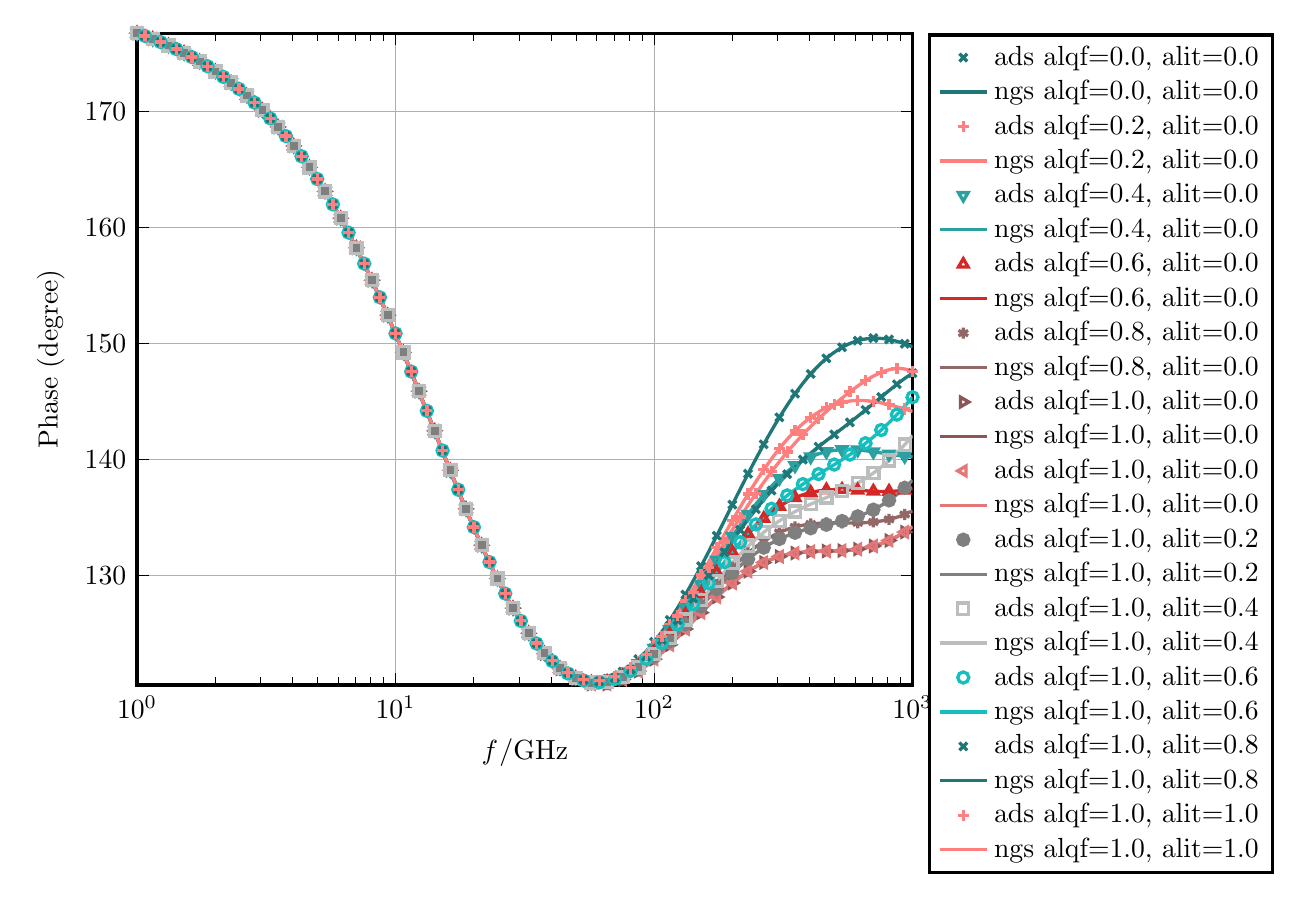
\begin{tikzpicture}[font=\normalsize]
\pgfplotsset{every axis/.append style={very thick}},
\definecolor{color0}{rgb}{0.12157, 0.46667, 0.46667}
\definecolor{color1}{rgb}{1.00000, 0.49804, 0.49804}
\definecolor{color2}{rgb}{0.17255, 0.62745, 0.62745}
\definecolor{color3}{rgb}{0.83922, 0.15294, 0.15294}
\definecolor{color4}{rgb}{0.58039, 0.40392, 0.40392}
\definecolor{color5}{rgb}{0.54902, 0.33725, 0.33725}
\definecolor{color6}{rgb}{0.89020, 0.46667, 0.46667}
\definecolor{color7}{rgb}{0.49804, 0.49804, 0.49804}
\definecolor{color8}{rgb}{0.73725, 0.74118, 0.74118}
\definecolor{color9}{rgb}{0.09020, 0.74510, 0.74510}

\begin{axis}[
width=4.5in,
xlabel={$f_{\mathrm{}}^{}/\si{\giga\hertz}$},
ylabel={Phase (degree)},
xmode=log,
% xmin=0,
% xmax=0,
% restrict x to domain=0:1,
log basis x=10,
% ymin=0,
% ymax=0,
% restrict y to domain=0:1,
log basis y=10,
xmajorgrids,
enlargelimits=false,
scaled ticks=false,
ymajorgrids,
x tick style={color=black},
y tick style={color=black},
x grid style={white!69.01960784313725!black},
y grid style={white!69.01960784313725!black},
/tikz/mark repeat=2,
legend style={at={(1.02,1.00)}, anchor=north west,legend cell align=left, align=left},
]
\addplot [color=color0, only marks, mark=x, mark options={solid}, mark phase=0, ]
  table[row sep=crcr, x expr=\thisrowno{0}*1.000000e-09, y expr=\thisrowno{1}*1.000000e+00]{
1e+09 176.713\\
1.07227e+09 176.476\\
1.14976e+09 176.222\\
1.23285e+09 175.951\\
1.32194e+09 175.659\\
1.41747e+09 175.347\\
1.51991e+09 175.013\\
1.62975e+09 174.655\\
1.74753e+09 174.272\\
1.87382e+09 173.862\\
2.00923e+09 173.423\\
2.15443e+09 172.953\\
2.31013e+09 172.451\\
2.47708e+09 171.914\\
2.65609e+09 171.34\\
2.84804e+09 170.728\\
3.05386e+09 170.074\\
3.27455e+09 169.376\\
3.51119e+09 168.633\\
3.76494e+09 167.841\\
4.03702e+09 166.999\\
4.32876e+09 166.104\\
4.64159e+09 165.154\\
4.97702e+09 164.148\\
5.3367e+09 163.083\\
5.72237e+09 161.958\\
6.13591e+09 160.773\\
6.57933e+09 159.526\\
7.0548e+09 158.219\\
7.56463e+09 156.852\\
8.11131e+09 155.426\\
8.69749e+09 153.944\\
9.32603e+09 152.411\\
1e+10 150.83\\
1.07227e+10 149.207\\
1.14976e+10 147.549\\
1.23285e+10 145.863\\
1.32194e+10 144.16\\
1.41747e+10 142.447\\
1.51991e+10 140.737\\
1.62975e+10 139.038\\
1.74753e+10 137.363\\
1.87382e+10 135.723\\
2.00923e+10 134.128\\
2.15443e+10 132.589\\
2.31013e+10 131.116\\
2.47708e+10 129.718\\
2.65609e+10 128.403\\
2.84804e+10 127.179\\
3.05386e+10 126.052\\
3.27455e+10 125.028\\
3.51119e+10 124.111\\
3.76494e+10 123.305\\
4.03702e+10 122.613\\
4.32876e+10 122.038\\
4.64159e+10 121.581\\
4.97702e+10 121.242\\
5.3367e+10 121.024\\
5.72237e+10 120.924\\
6.13591e+10 120.944\\
6.57933e+10 121.083\\
7.0548e+10 121.338\\
7.56463e+10 121.708\\
8.11131e+10 122.19\\
8.69749e+10 122.781\\
9.32603e+10 123.478\\
1e+11 124.276\\
1.07227e+11 125.168\\
1.14976e+11 126.15\\
1.23285e+11 127.212\\
1.32194e+11 128.347\\
1.41747e+11 129.545\\
1.51991e+11 130.796\\
1.62975e+11 132.089\\
1.74753e+11 133.412\\
1.87382e+11 134.752\\
2.00923e+11 136.098\\
2.15443e+11 137.437\\
2.31013e+11 138.757\\
2.47708e+11 140.045\\
2.65609e+11 141.29\\
2.84804e+11 142.483\\
3.05386e+11 143.613\\
3.27455e+11 144.672\\
3.51119e+11 145.653\\
3.76494e+11 146.551\\
4.03702e+11 147.36\\
4.32876e+11 148.076\\
4.64159e+11 148.697\\
4.97702e+11 149.222\\
5.3367e+11 149.651\\
5.72237e+11 149.984\\
6.13591e+11 150.224\\
6.57933e+11 150.373\\
7.0548e+11 150.436\\
7.56463e+11 150.419\\
8.11131e+11 150.328\\
8.69749e+11 150.171\\
9.32603e+11 149.956\\
1e+12 149.694\\
};
\addlegendentry{ads alqf=0.0, alit=0.0}
\addplot [color=color0, solid,  mark phase=0, ]
  table[row sep=crcr, x expr=\thisrowno{0}*1.000000e-09, y expr=\thisrowno{1}*1.000000e+00]{
1e+09 176.705\\
1.02306e+09 176.63\\
1.04665e+09 176.552\\
1.07079e+09 176.473\\
1.09548e+09 176.392\\
1.12074e+09 176.309\\
1.14658e+09 176.224\\
1.17302e+09 176.137\\
1.20007e+09 176.048\\
1.22775e+09 175.958\\
1.25606e+09 175.865\\
1.28502e+09 175.77\\
1.31466e+09 175.673\\
1.34497e+09 175.574\\
1.37599e+09 175.472\\
1.40772e+09 175.368\\
1.44018e+09 175.262\\
1.47339e+09 175.153\\
1.50736e+09 175.042\\
1.54212e+09 174.929\\
1.57768e+09 174.812\\
1.61406e+09 174.694\\
1.65128e+09 174.572\\
1.68936e+09 174.448\\
1.72832e+09 174.321\\
1.76817e+09 174.191\\
1.80895e+09 174.058\\
1.85066e+09 173.923\\
1.89334e+09 173.784\\
1.937e+09 173.642\\
1.98166e+09 173.497\\
2.02736e+09 173.349\\
2.07411e+09 173.197\\
2.12194e+09 173.042\\
2.17087e+09 172.883\\
2.22093e+09 172.722\\
2.27214e+09 172.556\\
2.32454e+09 172.387\\
2.37814e+09 172.214\\
2.43298e+09 172.037\\
2.48908e+09 171.857\\
2.54648e+09 171.672\\
2.6052e+09 171.484\\
2.66528e+09 171.291\\
2.72674e+09 171.094\\
2.78962e+09 170.893\\
2.85394e+09 170.687\\
2.91976e+09 170.478\\
2.98708e+09 170.263\\
3.05597e+09 170.044\\
3.12644e+09 169.821\\
3.19853e+09 169.592\\
3.27229e+09 169.359\\
3.34775e+09 169.121\\
3.42494e+09 168.878\\
3.50392e+09 168.63\\
3.58472e+09 168.376\\
3.66738e+09 168.118\\
3.75195e+09 167.854\\
3.83847e+09 167.585\\
3.92699e+09 167.31\\
4.01754e+09 167.03\\
4.11019e+09 166.744\\
4.20496e+09 166.452\\
4.30193e+09 166.155\\
4.40113e+09 165.852\\
4.50262e+09 165.543\\
4.60645e+09 165.227\\
4.71267e+09 164.906\\
4.82135e+09 164.579\\
4.93253e+09 164.246\\
5.04627e+09 163.906\\
5.16263e+09 163.56\\
5.28168e+09 163.208\\
5.40348e+09 162.849\\
5.52808e+09 162.484\\
5.65556e+09 162.113\\
5.78597e+09 161.735\\
5.91939e+09 161.35\\
6.05589e+09 160.959\\
6.19554e+09 160.562\\
6.33841e+09 160.158\\
6.48457e+09 159.747\\
6.6341e+09 159.33\\
6.78708e+09 158.906\\
6.94359e+09 158.476\\
7.10371e+09 158.04\\
7.26752e+09 157.597\\
7.43511e+09 157.148\\
7.60656e+09 156.692\\
7.78196e+09 156.231\\
7.96141e+09 155.763\\
8.145e+09 155.289\\
8.33282e+09 154.809\\
8.52497e+09 154.323\\
8.72156e+09 153.832\\
8.92267e+09 153.335\\
9.12843e+09 152.833\\
9.33893e+09 152.326\\
9.55428e+09 151.813\\
9.7746e+09 151.296\\
1e+10 150.774\\
1.02306e+10 150.247\\
1.04665e+10 149.716\\
1.07079e+10 149.181\\
1.09548e+10 148.643\\
1.12074e+10 148.101\\
1.14658e+10 147.556\\
1.17302e+10 147.008\\
1.20007e+10 146.457\\
1.22775e+10 145.904\\
1.25606e+10 145.349\\
1.28502e+10 144.792\\
1.31466e+10 144.234\\
1.34497e+10 143.675\\
1.37599e+10 143.115\\
1.40772e+10 142.555\\
1.44018e+10 141.995\\
1.47339e+10 141.436\\
1.50736e+10 140.877\\
1.54212e+10 140.32\\
1.57768e+10 139.764\\
1.61406e+10 139.21\\
1.65128e+10 138.659\\
1.68936e+10 138.11\\
1.72832e+10 137.564\\
1.76817e+10 137.022\\
1.80895e+10 136.484\\
1.85066e+10 135.95\\
1.89334e+10 135.421\\
1.937e+10 134.897\\
1.98166e+10 134.379\\
2.02736e+10 133.866\\
2.07411e+10 133.359\\
2.12194e+10 132.859\\
2.17087e+10 132.365\\
2.22093e+10 131.879\\
2.27214e+10 131.401\\
2.32454e+10 130.93\\
2.37814e+10 130.467\\
2.43298e+10 130.013\\
2.48908e+10 129.567\\
2.54648e+10 129.13\\
2.6052e+10 128.703\\
2.66528e+10 128.285\\
2.72674e+10 127.877\\
2.78962e+10 127.479\\
2.85394e+10 127.091\\
2.91976e+10 126.713\\
2.98708e+10 126.346\\
3.05597e+10 125.99\\
3.12644e+10 125.645\\
3.19853e+10 125.311\\
3.27229e+10 124.988\\
3.34775e+10 124.677\\
3.42494e+10 124.377\\
3.50392e+10 124.089\\
3.58472e+10 123.813\\
3.66738e+10 123.549\\
3.75195e+10 123.297\\
3.83847e+10 123.058\\
3.92699e+10 122.83\\
4.01754e+10 122.615\\
4.11019e+10 122.412\\
4.20496e+10 122.222\\
4.30193e+10 122.044\\
4.40113e+10 121.879\\
4.50262e+10 121.726\\
4.60645e+10 121.586\\
4.71267e+10 121.459\\
4.82135e+10 121.344\\
4.93253e+10 121.243\\
5.04627e+10 121.154\\
5.16263e+10 121.077\\
5.28168e+10 121.014\\
5.40348e+10 120.963\\
5.52808e+10 120.925\\
5.65556e+10 120.9\\
5.78597e+10 120.888\\
5.91939e+10 120.888\\
6.05589e+10 120.901\\
6.19554e+10 120.926\\
6.33841e+10 120.965\\
6.48457e+10 121.015\\
6.6341e+10 121.078\\
6.78708e+10 121.154\\
6.94359e+10 121.242\\
7.10371e+10 121.342\\
7.26752e+10 121.455\\
7.43511e+10 121.58\\
7.60656e+10 121.717\\
7.78196e+10 121.865\\
7.96141e+10 122.026\\
8.145e+10 122.199\\
8.33282e+10 122.383\\
8.52497e+10 122.578\\
8.72156e+10 122.785\\
8.92267e+10 123.003\\
9.12843e+10 123.232\\
9.33893e+10 123.472\\
9.55428e+10 123.723\\
9.7746e+10 123.985\\
1e+11 124.256\\
1.02306e+11 124.538\\
1.04665e+11 124.83\\
1.07079e+11 125.132\\
1.09548e+11 125.443\\
1.12074e+11 125.763\\
1.14658e+11 126.092\\
1.17302e+11 126.43\\
1.20007e+11 126.776\\
1.22775e+11 127.131\\
1.25606e+11 127.493\\
1.28502e+11 127.863\\
1.31466e+11 128.239\\
1.34497e+11 128.623\\
1.37599e+11 129.013\\
1.40772e+11 129.41\\
1.44018e+11 129.812\\
1.47339e+11 130.219\\
1.50736e+11 130.632\\
1.54212e+11 131.049\\
1.57768e+11 131.47\\
1.61406e+11 131.895\\
1.65128e+11 132.323\\
1.68936e+11 132.755\\
1.72832e+11 133.189\\
1.76817e+11 133.625\\
1.80895e+11 134.063\\
1.85066e+11 134.501\\
1.89334e+11 134.941\\
1.937e+11 135.381\\
1.98166e+11 135.821\\
2.02736e+11 136.261\\
2.07411e+11 136.7\\
2.12194e+11 137.137\\
2.17087e+11 137.572\\
2.22093e+11 138.005\\
2.27214e+11 138.436\\
2.32454e+11 138.863\\
2.37814e+11 139.287\\
2.43298e+11 139.708\\
2.48908e+11 140.123\\
2.54648e+11 140.535\\
2.6052e+11 140.941\\
2.66528e+11 141.342\\
2.72674e+11 141.737\\
2.78962e+11 142.126\\
2.85394e+11 142.509\\
2.91976e+11 142.885\\
2.98708e+11 143.254\\
3.05597e+11 143.615\\
3.12644e+11 143.97\\
3.19853e+11 144.316\\
3.27229e+11 144.654\\
3.34775e+11 144.984\\
3.42494e+11 145.305\\
3.50392e+11 145.618\\
3.58472e+11 145.921\\
3.66738e+11 146.216\\
3.75195e+11 146.501\\
3.83847e+11 146.777\\
3.92699e+11 147.043\\
4.01754e+11 147.299\\
4.11019e+11 147.546\\
4.20496e+11 147.782\\
4.30193e+11 148.009\\
4.40113e+11 148.225\\
4.50262e+11 148.431\\
4.60645e+11 148.627\\
4.71267e+11 148.813\\
4.82135e+11 148.988\\
4.93253e+11 149.153\\
5.04627e+11 149.308\\
5.16263e+11 149.452\\
5.28168e+11 149.586\\
5.40348e+11 149.71\\
5.52808e+11 149.824\\
5.65556e+11 149.928\\
5.78597e+11 150.022\\
5.91939e+11 150.105\\
6.05589e+11 150.179\\
6.19554e+11 150.243\\
6.33841e+11 150.298\\
6.48457e+11 150.343\\
6.6341e+11 150.379\\
6.78708e+11 150.405\\
6.94359e+11 150.423\\
7.10371e+11 150.432\\
7.26752e+11 150.433\\
7.43511e+11 150.425\\
7.60656e+11 150.409\\
7.78196e+11 150.385\\
7.96141e+11 150.354\\
8.145e+11 150.315\\
8.33282e+11 150.27\\
8.52497e+11 150.217\\
8.72156e+11 150.158\\
8.92267e+11 150.093\\
9.12843e+11 150.023\\
9.33893e+11 149.947\\
9.55428e+11 149.866\\
9.7746e+11 149.78\\
1e+12 149.69\\
};
\addlegendentry{ngs alqf=0.0, alit=0.0}
\addplot [color=color1, only marks, mark=+, mark options={solid}, mark phase=0, ]
  table[row sep=crcr, x expr=\thisrowno{0}*1.000000e-09, y expr=\thisrowno{1}*1.000000e+00]{
1e+09 176.713\\
1.07227e+09 176.476\\
1.14976e+09 176.222\\
1.23285e+09 175.951\\
1.32194e+09 175.659\\
1.41747e+09 175.347\\
1.51991e+09 175.013\\
1.62975e+09 174.655\\
1.74753e+09 174.272\\
1.87382e+09 173.862\\
2.00923e+09 173.423\\
2.15443e+09 172.953\\
2.31013e+09 172.451\\
2.47708e+09 171.914\\
2.65609e+09 171.34\\
2.84804e+09 170.728\\
3.05386e+09 170.074\\
3.27455e+09 169.376\\
3.51119e+09 168.633\\
3.76494e+09 167.841\\
4.03702e+09 166.999\\
4.32876e+09 166.104\\
4.64159e+09 165.154\\
4.97702e+09 164.148\\
5.3367e+09 163.083\\
5.72237e+09 161.958\\
6.13591e+09 160.773\\
6.57933e+09 159.527\\
7.0548e+09 158.219\\
7.56463e+09 156.852\\
8.11131e+09 155.426\\
8.69749e+09 153.945\\
9.32603e+09 152.411\\
1e+10 150.83\\
1.07227e+10 149.208\\
1.14976e+10 147.55\\
1.23285e+10 145.865\\
1.32194e+10 144.161\\
1.41747e+10 142.449\\
1.51991e+10 140.738\\
1.62975e+10 139.04\\
1.74753e+10 137.365\\
1.87382e+10 135.725\\
2.00923e+10 134.13\\
2.15443e+10 132.591\\
2.31013e+10 131.118\\
2.47708e+10 129.719\\
2.65609e+10 128.404\\
2.84804e+10 127.179\\
3.05386e+10 126.051\\
3.27455e+10 125.026\\
3.51119e+10 124.107\\
3.76494e+10 123.298\\
4.03702e+10 122.603\\
4.32876e+10 122.024\\
4.64159e+10 121.561\\
4.97702e+10 121.216\\
5.3367e+10 120.988\\
5.72237e+10 120.879\\
6.13591e+10 120.886\\
6.57933e+10 121.008\\
7.0548e+10 121.244\\
7.56463e+10 121.59\\
8.11131e+10 122.044\\
8.69749e+10 122.602\\
9.32603e+10 123.258\\
1e+11 124.008\\
1.07227e+11 124.845\\
1.14976e+11 125.761\\
1.23285e+11 126.747\\
1.32194e+11 127.795\\
1.41747e+11 128.893\\
1.51991e+11 130.031\\
1.62975e+11 131.197\\
1.74753e+11 132.379\\
1.87382e+11 133.563\\
2.00923e+11 134.737\\
2.15443e+11 135.889\\
2.31013e+11 137.008\\
2.47708e+11 138.08\\
2.65609e+11 139.098\\
2.84804e+11 140.05\\
3.05386e+11 140.931\\
3.27455e+11 141.732\\
3.51119e+11 142.45\\
3.76494e+11 143.081\\
4.03702e+11 143.622\\
4.32876e+11 144.074\\
4.64159e+11 144.438\\
4.97702e+11 144.715\\
5.3367e+11 144.91\\
5.72237e+11 145.028\\
6.13591e+11 145.075\\
6.57933e+11 145.059\\
7.0548e+11 144.987\\
7.56463e+11 144.868\\
8.11131e+11 144.713\\
8.69749e+11 144.531\\
9.32603e+11 144.333\\
1e+12 144.129\\
};
\addlegendentry{ads alqf=0.2, alit=0.0}
\addplot [color=color1, solid,  mark phase=0, ]
  table[row sep=crcr, x expr=\thisrowno{0}*1.000000e-09, y expr=\thisrowno{1}*1.000000e+00]{
1e+09 176.705\\
1.02306e+09 176.63\\
1.04665e+09 176.552\\
1.07079e+09 176.473\\
1.09548e+09 176.392\\
1.12074e+09 176.309\\
1.14658e+09 176.224\\
1.17302e+09 176.137\\
1.20007e+09 176.048\\
1.22775e+09 175.958\\
1.25606e+09 175.865\\
1.28502e+09 175.77\\
1.31466e+09 175.673\\
1.34497e+09 175.574\\
1.37599e+09 175.472\\
1.40772e+09 175.368\\
1.44018e+09 175.262\\
1.47339e+09 175.153\\
1.50736e+09 175.042\\
1.54212e+09 174.929\\
1.57768e+09 174.812\\
1.61406e+09 174.694\\
1.65128e+09 174.572\\
1.68936e+09 174.448\\
1.72832e+09 174.321\\
1.76817e+09 174.191\\
1.80895e+09 174.058\\
1.85066e+09 173.923\\
1.89334e+09 173.784\\
1.937e+09 173.642\\
1.98166e+09 173.497\\
2.02736e+09 173.349\\
2.07411e+09 173.197\\
2.12194e+09 173.042\\
2.17087e+09 172.883\\
2.22093e+09 172.722\\
2.27214e+09 172.556\\
2.32454e+09 172.387\\
2.37814e+09 172.214\\
2.43298e+09 172.037\\
2.48908e+09 171.857\\
2.54648e+09 171.672\\
2.6052e+09 171.484\\
2.66528e+09 171.291\\
2.72674e+09 171.094\\
2.78962e+09 170.893\\
2.85394e+09 170.687\\
2.91976e+09 170.478\\
2.98708e+09 170.263\\
3.05597e+09 170.044\\
3.12644e+09 169.821\\
3.19853e+09 169.592\\
3.27229e+09 169.359\\
3.34775e+09 169.121\\
3.42494e+09 168.878\\
3.50392e+09 168.63\\
3.58472e+09 168.376\\
3.66738e+09 168.118\\
3.75195e+09 167.854\\
3.83847e+09 167.585\\
3.92699e+09 167.31\\
4.01754e+09 167.03\\
4.11019e+09 166.744\\
4.20496e+09 166.452\\
4.30193e+09 166.155\\
4.40113e+09 165.852\\
4.50262e+09 165.543\\
4.60645e+09 165.228\\
4.71267e+09 164.906\\
4.82135e+09 164.579\\
4.93253e+09 164.246\\
5.04627e+09 163.906\\
5.16263e+09 163.56\\
5.28168e+09 163.208\\
5.40348e+09 162.849\\
5.52808e+09 162.484\\
5.65556e+09 162.113\\
5.78597e+09 161.735\\
5.91939e+09 161.35\\
6.05589e+09 160.959\\
6.19554e+09 160.562\\
6.33841e+09 160.158\\
6.48457e+09 159.747\\
6.6341e+09 159.33\\
6.78708e+09 158.907\\
6.94359e+09 158.477\\
7.10371e+09 158.04\\
7.26752e+09 157.597\\
7.43511e+09 157.148\\
7.60656e+09 156.693\\
7.78196e+09 156.231\\
7.96141e+09 155.763\\
8.145e+09 155.289\\
8.33282e+09 154.81\\
8.52497e+09 154.324\\
8.72156e+09 153.833\\
8.92267e+09 153.336\\
9.12843e+09 152.834\\
9.33893e+09 152.326\\
9.55428e+09 151.814\\
9.7746e+09 151.296\\
1e+10 150.774\\
1.02306e+10 150.248\\
1.04665e+10 149.717\\
1.07079e+10 149.182\\
1.09548e+10 148.644\\
1.12074e+10 148.102\\
1.14658e+10 147.557\\
1.17302e+10 147.009\\
1.20007e+10 146.458\\
1.22775e+10 145.905\\
1.25606e+10 145.35\\
1.28502e+10 144.793\\
1.31466e+10 144.235\\
1.34497e+10 143.676\\
1.37599e+10 143.117\\
1.40772e+10 142.557\\
1.44018e+10 141.997\\
1.47339e+10 141.438\\
1.50736e+10 140.879\\
1.54212e+10 140.322\\
1.57768e+10 139.766\\
1.61406e+10 139.212\\
1.65128e+10 138.661\\
1.68936e+10 138.112\\
1.72832e+10 137.566\\
1.76817e+10 137.024\\
1.80895e+10 136.486\\
1.85066e+10 135.953\\
1.89334e+10 135.423\\
1.937e+10 134.899\\
1.98166e+10 134.381\\
2.02736e+10 133.868\\
2.07411e+10 133.361\\
2.12194e+10 132.861\\
2.17087e+10 132.367\\
2.22093e+10 131.881\\
2.27214e+10 131.402\\
2.32454e+10 130.932\\
2.37814e+10 130.469\\
2.43298e+10 130.014\\
2.48908e+10 129.568\\
2.54648e+10 129.132\\
2.6052e+10 128.704\\
2.66528e+10 128.286\\
2.72674e+10 127.878\\
2.78962e+10 127.479\\
2.85394e+10 127.091\\
2.91976e+10 126.713\\
2.98708e+10 126.346\\
3.05597e+10 125.989\\
3.12644e+10 125.644\\
3.19853e+10 125.309\\
3.27229e+10 124.986\\
3.34775e+10 124.674\\
3.42494e+10 124.374\\
3.50392e+10 124.085\\
3.58472e+10 123.808\\
3.66738e+10 123.544\\
3.75195e+10 123.291\\
3.83847e+10 123.05\\
3.92699e+10 122.821\\
4.01754e+10 122.605\\
4.11019e+10 122.401\\
4.20496e+10 122.209\\
4.30193e+10 122.03\\
4.40113e+10 121.863\\
4.50262e+10 121.709\\
4.60645e+10 121.567\\
4.71267e+10 121.438\\
4.82135e+10 121.321\\
4.93253e+10 121.217\\
5.04627e+10 121.125\\
5.16263e+10 121.046\\
5.28168e+10 120.98\\
5.40348e+10 120.926\\
5.52808e+10 120.885\\
5.65556e+10 120.856\\
5.78597e+10 120.84\\
5.91939e+10 120.836\\
6.05589e+10 120.844\\
6.19554e+10 120.865\\
6.33841e+10 120.898\\
6.48457e+10 120.944\\
6.6341e+10 121.001\\
6.78708e+10 121.071\\
6.94359e+10 121.152\\
7.10371e+10 121.246\\
7.26752e+10 121.351\\
7.43511e+10 121.468\\
7.60656e+10 121.597\\
7.78196e+10 121.737\\
7.96141e+10 121.888\\
8.145e+10 122.05\\
8.33282e+10 122.224\\
8.52497e+10 122.408\\
8.72156e+10 122.603\\
8.92267e+10 122.809\\
9.12843e+10 123.025\\
9.33893e+10 123.251\\
9.55428e+10 123.487\\
9.7746e+10 123.733\\
1e+11 123.988\\
1.02306e+11 124.253\\
1.04665e+11 124.526\\
1.07079e+11 124.809\\
1.09548e+11 125.099\\
1.12074e+11 125.398\\
1.14658e+11 125.705\\
1.17302e+11 126.02\\
1.20007e+11 126.341\\
1.22775e+11 126.67\\
1.25606e+11 127.005\\
1.28502e+11 127.347\\
1.31466e+11 127.694\\
1.34497e+11 128.047\\
1.37599e+11 128.405\\
1.40772e+11 128.768\\
1.44018e+11 129.135\\
1.47339e+11 129.506\\
1.50736e+11 129.88\\
1.54212e+11 130.258\\
1.57768e+11 130.638\\
1.61406e+11 131.021\\
1.65128e+11 131.406\\
1.68936e+11 131.791\\
1.72832e+11 132.178\\
1.76817e+11 132.566\\
1.80895e+11 132.953\\
1.85066e+11 133.34\\
1.89334e+11 133.726\\
1.937e+11 134.111\\
1.98166e+11 134.494\\
2.02736e+11 134.876\\
2.07411e+11 135.254\\
2.12194e+11 135.63\\
2.17087e+11 136.002\\
2.22093e+11 136.371\\
2.27214e+11 136.735\\
2.32454e+11 137.095\\
2.37814e+11 137.449\\
2.43298e+11 137.799\\
2.48908e+11 138.143\\
2.54648e+11 138.48\\
2.6052e+11 138.812\\
2.66528e+11 139.137\\
2.72674e+11 139.454\\
2.78962e+11 139.765\\
2.85394e+11 140.068\\
2.91976e+11 140.363\\
2.98708e+11 140.651\\
3.05597e+11 140.93\\
3.12644e+11 141.201\\
3.19853e+11 141.463\\
3.27229e+11 141.716\\
3.34775e+11 141.96\\
3.42494e+11 142.195\\
3.50392e+11 142.421\\
3.58472e+11 142.638\\
3.66738e+11 142.845\\
3.75195e+11 143.043\\
3.83847e+11 143.231\\
3.92699e+11 143.41\\
4.01754e+11 143.579\\
4.11019e+11 143.739\\
4.20496e+11 143.889\\
4.30193e+11 144.029\\
4.40113e+11 144.16\\
4.50262e+11 144.282\\
4.60645e+11 144.394\\
4.71267e+11 144.497\\
4.82135e+11 144.591\\
4.93253e+11 144.676\\
5.04627e+11 144.752\\
5.16263e+11 144.82\\
5.28168e+11 144.879\\
5.40348e+11 144.929\\
5.52808e+11 144.972\\
5.65556e+11 145.006\\
5.78597e+11 145.033\\
5.91939e+11 145.052\\
6.05589e+11 145.064\\
6.19554e+11 145.07\\
6.33841e+11 145.068\\
6.48457e+11 145.06\\
6.6341e+11 145.046\\
6.78708e+11 145.027\\
6.94359e+11 145.001\\
7.10371e+11 144.971\\
7.26752e+11 144.936\\
7.43511e+11 144.896\\
7.60656e+11 144.852\\
7.78196e+11 144.804\\
7.96141e+11 144.752\\
8.145e+11 144.698\\
8.33282e+11 144.641\\
8.52497e+11 144.581\\
8.72156e+11 144.519\\
8.92267e+11 144.456\\
9.12843e+11 144.391\\
9.33893e+11 144.325\\
9.55428e+11 144.259\\
9.7746e+11 144.193\\
1e+12 144.127\\
};
\addlegendentry{ngs alqf=0.2, alit=0.0}
\addplot [color=color2, only marks, mark=triangle, mark options={solid, rotate=180}, mark phase=0, ]
  table[row sep=crcr, x expr=\thisrowno{0}*1.000000e-09, y expr=\thisrowno{1}*1.000000e+00]{
1e+09 176.713\\
1.07227e+09 176.476\\
1.14976e+09 176.222\\
1.23285e+09 175.951\\
1.32194e+09 175.659\\
1.41747e+09 175.347\\
1.51991e+09 175.013\\
1.62975e+09 174.655\\
1.74753e+09 174.272\\
1.87382e+09 173.862\\
2.00923e+09 173.423\\
2.15443e+09 172.953\\
2.31013e+09 172.451\\
2.47708e+09 171.914\\
2.65609e+09 171.34\\
2.84804e+09 170.728\\
3.05386e+09 170.074\\
3.27455e+09 169.376\\
3.51119e+09 168.633\\
3.76494e+09 167.841\\
4.03702e+09 166.999\\
4.32876e+09 166.104\\
4.64159e+09 165.155\\
4.97702e+09 164.148\\
5.3367e+09 163.083\\
5.72237e+09 161.959\\
6.13591e+09 160.773\\
6.57933e+09 159.527\\
7.0548e+09 158.22\\
7.56463e+09 156.852\\
8.11131e+09 155.427\\
8.69749e+09 153.946\\
9.32603e+09 152.412\\
1e+10 150.831\\
1.07227e+10 149.208\\
1.14976e+10 147.551\\
1.23285e+10 145.866\\
1.32194e+10 144.163\\
1.41747e+10 142.451\\
1.51991e+10 140.74\\
1.62975e+10 139.042\\
1.74753e+10 137.367\\
1.87382e+10 135.727\\
2.00923e+10 134.132\\
2.15443e+10 132.593\\
2.31013e+10 131.119\\
2.47708e+10 129.72\\
2.65609e+10 128.404\\
2.84804e+10 127.179\\
3.05386e+10 126.05\\
3.27455e+10 125.022\\
3.51119e+10 124.101\\
3.76494e+10 123.29\\
4.03702e+10 122.591\\
4.32876e+10 122.007\\
4.64159e+10 121.538\\
4.97702e+10 121.186\\
5.3367e+10 120.949\\
5.72237e+10 120.828\\
6.13591e+10 120.821\\
6.57933e+10 120.926\\
7.0548e+10 121.141\\
7.56463e+10 121.462\\
8.11131e+10 121.886\\
8.69749e+10 122.408\\
9.32603e+10 123.023\\
1e+11 123.723\\
1.07227e+11 124.501\\
1.14976e+11 125.349\\
1.23285e+11 126.258\\
1.32194e+11 127.217\\
1.41747e+11 128.215\\
1.51991e+11 129.24\\
1.62975e+11 130.281\\
1.74753e+11 131.323\\
1.87382e+11 132.355\\
2.00923e+11 133.365\\
2.15443e+11 134.341\\
2.31013e+11 135.271\\
2.47708e+11 136.147\\
2.65609e+11 136.958\\
2.84804e+11 137.699\\
3.05386e+11 138.364\\
3.27455e+11 138.948\\
3.51119e+11 139.451\\
3.76494e+11 139.87\\
4.03702e+11 140.209\\
4.32876e+11 140.469\\
4.64159e+11 140.657\\
4.97702e+11 140.776\\
5.3367e+11 140.836\\
5.72237e+11 140.845\\
6.13591e+11 140.81\\
6.57933e+11 140.743\\
7.0548e+11 140.653\\
7.56463e+11 140.551\\
8.11131e+11 140.446\\
8.69749e+11 140.348\\
9.32603e+11 140.267\\
1e+12 140.212\\
};
\addlegendentry{ads alqf=0.4, alit=0.0}
\addplot [color=color2, solid,  mark phase=0, ]
  table[row sep=crcr, x expr=\thisrowno{0}*1.000000e-09, y expr=\thisrowno{1}*1.000000e+00]{
1e+09 176.705\\
1.02306e+09 176.63\\
1.04665e+09 176.552\\
1.07079e+09 176.473\\
1.09548e+09 176.392\\
1.12074e+09 176.309\\
1.14658e+09 176.224\\
1.17302e+09 176.137\\
1.20007e+09 176.048\\
1.22775e+09 175.958\\
1.25606e+09 175.865\\
1.28502e+09 175.77\\
1.31466e+09 175.673\\
1.34497e+09 175.574\\
1.37599e+09 175.472\\
1.40772e+09 175.368\\
1.44018e+09 175.262\\
1.47339e+09 175.153\\
1.50736e+09 175.042\\
1.54212e+09 174.929\\
1.57768e+09 174.812\\
1.61406e+09 174.694\\
1.65128e+09 174.572\\
1.68936e+09 174.448\\
1.72832e+09 174.321\\
1.76817e+09 174.191\\
1.80895e+09 174.058\\
1.85066e+09 173.923\\
1.89334e+09 173.784\\
1.937e+09 173.642\\
1.98166e+09 173.497\\
2.02736e+09 173.349\\
2.07411e+09 173.197\\
2.12194e+09 173.042\\
2.17087e+09 172.884\\
2.22093e+09 172.722\\
2.27214e+09 172.556\\
2.32454e+09 172.387\\
2.37814e+09 172.214\\
2.43298e+09 172.037\\
2.48908e+09 171.857\\
2.54648e+09 171.672\\
2.6052e+09 171.484\\
2.66528e+09 171.291\\
2.72674e+09 171.094\\
2.78962e+09 170.893\\
2.85394e+09 170.688\\
2.91976e+09 170.478\\
2.98708e+09 170.263\\
3.05597e+09 170.044\\
3.12644e+09 169.821\\
3.19853e+09 169.592\\
3.27229e+09 169.359\\
3.34775e+09 169.121\\
3.42494e+09 168.878\\
3.50392e+09 168.63\\
3.58472e+09 168.376\\
3.66738e+09 168.118\\
3.75195e+09 167.854\\
3.83847e+09 167.585\\
3.92699e+09 167.31\\
4.01754e+09 167.03\\
4.11019e+09 166.744\\
4.20496e+09 166.452\\
4.30193e+09 166.155\\
4.40113e+09 165.852\\
4.50262e+09 165.543\\
4.60645e+09 165.228\\
4.71267e+09 164.906\\
4.82135e+09 164.579\\
4.93253e+09 164.246\\
5.04627e+09 163.906\\
5.16263e+09 163.56\\
5.28168e+09 163.208\\
5.40348e+09 162.849\\
5.52808e+09 162.484\\
5.65556e+09 162.113\\
5.78597e+09 161.735\\
5.91939e+09 161.351\\
6.05589e+09 160.96\\
6.19554e+09 160.562\\
6.33841e+09 160.158\\
6.48457e+09 159.748\\
6.6341e+09 159.331\\
6.78708e+09 158.907\\
6.94359e+09 158.477\\
7.10371e+09 158.041\\
7.26752e+09 157.598\\
7.43511e+09 157.149\\
7.60656e+09 156.693\\
7.78196e+09 156.232\\
7.96141e+09 155.764\\
8.145e+09 155.29\\
8.33282e+09 154.81\\
8.52497e+09 154.325\\
8.72156e+09 153.833\\
8.92267e+09 153.337\\
9.12843e+09 152.834\\
9.33893e+09 152.327\\
9.55428e+09 151.814\\
9.7746e+09 151.297\\
1e+10 150.775\\
1.02306e+10 150.249\\
1.04665e+10 149.718\\
1.07079e+10 149.183\\
1.09548e+10 148.645\\
1.12074e+10 148.103\\
1.14658e+10 147.558\\
1.17302e+10 147.01\\
1.20007e+10 146.459\\
1.22775e+10 145.906\\
1.25606e+10 145.351\\
1.28502e+10 144.795\\
1.31466e+10 144.237\\
1.34497e+10 143.678\\
1.37599e+10 143.118\\
1.40772e+10 142.558\\
1.44018e+10 141.998\\
1.47339e+10 141.439\\
1.50736e+10 140.881\\
1.54212e+10 140.323\\
1.57768e+10 139.767\\
1.61406e+10 139.214\\
1.65128e+10 138.662\\
1.68936e+10 138.114\\
1.72832e+10 137.568\\
1.76817e+10 137.026\\
1.80895e+10 136.488\\
1.85066e+10 135.954\\
1.89334e+10 135.425\\
1.937e+10 134.901\\
1.98166e+10 134.383\\
2.02736e+10 133.87\\
2.07411e+10 133.363\\
2.12194e+10 132.863\\
2.17087e+10 132.369\\
2.22093e+10 131.883\\
2.27214e+10 131.404\\
2.32454e+10 130.933\\
2.37814e+10 130.47\\
2.43298e+10 130.015\\
2.48908e+10 129.569\\
2.54648e+10 129.132\\
2.6052e+10 128.705\\
2.66528e+10 128.286\\
2.72674e+10 127.878\\
2.78962e+10 127.479\\
2.85394e+10 127.09\\
2.91976e+10 126.712\\
2.98708e+10 126.344\\
3.05597e+10 125.987\\
3.12644e+10 125.641\\
3.19853e+10 125.306\\
3.27229e+10 124.982\\
3.34775e+10 124.67\\
3.42494e+10 124.369\\
3.50392e+10 124.08\\
3.58472e+10 123.802\\
3.66738e+10 123.536\\
3.75195e+10 123.282\\
3.83847e+10 123.04\\
3.92699e+10 122.811\\
4.01754e+10 122.593\\
4.11019e+10 122.387\\
4.20496e+10 122.194\\
4.30193e+10 122.013\\
4.40113e+10 121.845\\
4.50262e+10 121.688\\
4.60645e+10 121.545\\
4.71267e+10 121.413\\
4.82135e+10 121.294\\
4.93253e+10 121.187\\
5.04627e+10 121.093\\
5.16263e+10 121.011\\
5.28168e+10 120.942\\
5.40348e+10 120.885\\
5.52808e+10 120.84\\
5.65556e+10 120.807\\
5.78597e+10 120.787\\
5.91939e+10 120.778\\
6.05589e+10 120.782\\
6.19554e+10 120.798\\
6.33841e+10 120.826\\
6.48457e+10 120.865\\
6.6341e+10 120.917\\
6.78708e+10 120.98\\
6.94359e+10 121.054\\
7.10371e+10 121.14\\
7.26752e+10 121.238\\
7.43511e+10 121.346\\
7.60656e+10 121.466\\
7.78196e+10 121.597\\
7.96141e+10 121.738\\
8.145e+10 121.89\\
8.33282e+10 122.053\\
8.52497e+10 122.225\\
8.72156e+10 122.408\\
8.92267e+10 122.6\\
9.12843e+10 122.802\\
9.33893e+10 123.014\\
9.55428e+10 123.234\\
9.7746e+10 123.464\\
1e+11 123.702\\
1.02306e+11 123.949\\
1.04665e+11 124.203\\
1.07079e+11 124.466\\
1.09548e+11 124.735\\
1.12074e+11 125.012\\
1.14658e+11 125.296\\
1.17302e+11 125.587\\
1.20007e+11 125.883\\
1.22775e+11 126.185\\
1.25606e+11 126.493\\
1.28502e+11 126.806\\
1.31466e+11 127.123\\
1.34497e+11 127.445\\
1.37599e+11 127.77\\
1.40772e+11 128.099\\
1.44018e+11 128.431\\
1.47339e+11 128.766\\
1.50736e+11 129.103\\
1.54212e+11 129.441\\
1.57768e+11 129.781\\
1.61406e+11 130.122\\
1.65128e+11 130.463\\
1.68936e+11 130.804\\
1.72832e+11 131.145\\
1.76817e+11 131.485\\
1.80895e+11 131.823\\
1.85066e+11 132.16\\
1.89334e+11 132.494\\
1.937e+11 132.826\\
1.98166e+11 133.155\\
2.02736e+11 133.481\\
2.07411e+11 133.802\\
2.12194e+11 134.12\\
2.17087e+11 134.433\\
2.22093e+11 134.741\\
2.27214e+11 135.043\\
2.32454e+11 135.34\\
2.37814e+11 135.631\\
2.43298e+11 135.916\\
2.48908e+11 136.194\\
2.54648e+11 136.465\\
2.6052e+11 136.729\\
2.66528e+11 136.986\\
2.72674e+11 137.235\\
2.78962e+11 137.476\\
2.85394e+11 137.71\\
2.91976e+11 137.935\\
2.98708e+11 138.152\\
3.05597e+11 138.36\\
3.12644e+11 138.56\\
3.19853e+11 138.751\\
3.27229e+11 138.933\\
3.34775e+11 139.107\\
3.42494e+11 139.271\\
3.50392e+11 139.427\\
3.58472e+11 139.574\\
3.66738e+11 139.712\\
3.75195e+11 139.842\\
3.83847e+11 139.963\\
3.92699e+11 140.075\\
4.01754e+11 140.179\\
4.11019e+11 140.274\\
4.20496e+11 140.361\\
4.30193e+11 140.44\\
4.40113e+11 140.512\\
4.50262e+11 140.575\\
4.60645e+11 140.631\\
4.71267e+11 140.68\\
4.82135e+11 140.722\\
4.93253e+11 140.756\\
5.04627e+11 140.785\\
5.16263e+11 140.807\\
5.28168e+11 140.823\\
5.40348e+11 140.834\\
5.52808e+11 140.839\\
5.65556e+11 140.839\\
5.78597e+11 140.835\\
5.91939e+11 140.826\\
6.05589e+11 140.813\\
6.19554e+11 140.796\\
6.33841e+11 140.776\\
6.48457e+11 140.753\\
6.6341e+11 140.728\\
6.78708e+11 140.7\\
6.94359e+11 140.67\\
7.10371e+11 140.638\\
7.26752e+11 140.606\\
7.43511e+11 140.572\\
7.60656e+11 140.538\\
7.78196e+11 140.504\\
7.96141e+11 140.47\\
8.145e+11 140.436\\
8.33282e+11 140.403\\
8.52497e+11 140.372\\
8.72156e+11 140.342\\
8.92267e+11 140.314\\
9.12843e+11 140.288\\
9.33893e+11 140.264\\
9.55428e+11 140.243\\
9.7746e+11 140.226\\
1e+12 140.212\\
};
\addlegendentry{ngs alqf=0.4, alit=0.0}
\addplot [color=color3, only marks, mark=triangle, mark options={solid, rotate=0}, mark phase=0, ]
  table[row sep=crcr, x expr=\thisrowno{0}*1.000000e-09, y expr=\thisrowno{1}*1.000000e+00]{
1e+09 176.713\\
1.07227e+09 176.476\\
1.14976e+09 176.222\\
1.23285e+09 175.951\\
1.32194e+09 175.659\\
1.41747e+09 175.347\\
1.51991e+09 175.013\\
1.62975e+09 174.655\\
1.74753e+09 174.272\\
1.87382e+09 173.862\\
2.00923e+09 173.423\\
2.15443e+09 172.953\\
2.31013e+09 172.451\\
2.47708e+09 171.914\\
2.65609e+09 171.341\\
2.84804e+09 170.728\\
3.05386e+09 170.074\\
3.27455e+09 169.376\\
3.51119e+09 168.633\\
3.76494e+09 167.841\\
4.03702e+09 166.999\\
4.32876e+09 166.104\\
4.64159e+09 165.155\\
4.97702e+09 164.148\\
5.3367e+09 163.083\\
5.72237e+09 161.959\\
6.13591e+09 160.774\\
6.57933e+09 159.527\\
7.0548e+09 158.22\\
7.56463e+09 156.853\\
8.11131e+09 155.427\\
8.69749e+09 153.946\\
9.32603e+09 152.413\\
1e+10 150.832\\
1.07227e+10 149.209\\
1.14976e+10 147.552\\
1.23285e+10 145.867\\
1.32194e+10 144.164\\
1.41747e+10 142.452\\
1.51991e+10 140.742\\
1.62975e+10 139.044\\
1.74753e+10 137.369\\
1.87382e+10 135.729\\
2.00923e+10 134.134\\
2.15443e+10 132.594\\
2.31013e+10 131.12\\
2.47708e+10 129.721\\
2.65609e+10 128.404\\
2.84804e+10 127.178\\
3.05386e+10 126.047\\
3.27455e+10 125.018\\
3.51119e+10 124.095\\
3.76494e+10 123.28\\
4.03702e+10 122.577\\
4.32876e+10 121.988\\
4.64159e+10 121.513\\
4.97702e+10 121.152\\
5.3367e+10 120.905\\
5.72237e+10 120.772\\
6.13591e+10 120.75\\
6.57933e+10 120.837\\
7.0548e+10 121.03\\
7.56463e+10 121.325\\
8.11131e+10 121.717\\
8.69749e+10 122.202\\
9.32603e+10 122.772\\
1e+11 123.421\\
1.07227e+11 124.139\\
1.14976e+11 124.919\\
1.23285e+11 125.749\\
1.32194e+11 126.619\\
1.41747e+11 127.517\\
1.51991e+11 128.431\\
1.62975e+11 129.349\\
1.74753e+11 130.257\\
1.87382e+11 131.145\\
2.00923e+11 132\\
2.15443e+11 132.812\\
2.31013e+11 133.572\\
2.47708e+11 134.27\\
2.65609e+11 134.902\\
2.84804e+11 135.461\\
3.05386e+11 135.946\\
3.27455e+11 136.355\\
3.51119e+11 136.689\\
3.76494e+11 136.951\\
4.03702e+11 137.146\\
4.32876e+11 137.28\\
4.64159e+11 137.361\\
4.97702e+11 137.397\\
5.3367e+11 137.398\\
5.72237e+11 137.374\\
6.13591e+11 137.335\\
6.57933e+11 137.292\\
7.0548e+11 137.255\\
7.56463e+11 137.233\\
8.11131e+11 137.235\\
8.69749e+11 137.271\\
9.32603e+11 137.346\\
1e+12 137.468\\
};
\addlegendentry{ads alqf=0.6, alit=0.0}
\addplot [color=color3, solid,  mark phase=0, ]
  table[row sep=crcr, x expr=\thisrowno{0}*1.000000e-09, y expr=\thisrowno{1}*1.000000e+00]{
1e+09 176.705\\
1.02306e+09 176.63\\
1.04665e+09 176.552\\
1.07079e+09 176.473\\
1.09548e+09 176.392\\
1.12074e+09 176.309\\
1.14658e+09 176.224\\
1.17302e+09 176.137\\
1.20007e+09 176.048\\
1.22775e+09 175.958\\
1.25606e+09 175.865\\
1.28502e+09 175.77\\
1.31466e+09 175.673\\
1.34497e+09 175.574\\
1.37599e+09 175.472\\
1.40772e+09 175.368\\
1.44018e+09 175.262\\
1.47339e+09 175.153\\
1.50736e+09 175.042\\
1.54212e+09 174.929\\
1.57768e+09 174.813\\
1.61406e+09 174.694\\
1.65128e+09 174.572\\
1.68936e+09 174.448\\
1.72832e+09 174.321\\
1.76817e+09 174.191\\
1.80895e+09 174.058\\
1.85066e+09 173.923\\
1.89334e+09 173.784\\
1.937e+09 173.642\\
1.98166e+09 173.497\\
2.02736e+09 173.349\\
2.07411e+09 173.197\\
2.12194e+09 173.042\\
2.17087e+09 172.884\\
2.22093e+09 172.722\\
2.27214e+09 172.556\\
2.32454e+09 172.387\\
2.37814e+09 172.214\\
2.43298e+09 172.037\\
2.48908e+09 171.857\\
2.54648e+09 171.672\\
2.6052e+09 171.484\\
2.66528e+09 171.291\\
2.72674e+09 171.094\\
2.78962e+09 170.893\\
2.85394e+09 170.688\\
2.91976e+09 170.478\\
2.98708e+09 170.263\\
3.05597e+09 170.044\\
3.12644e+09 169.821\\
3.19853e+09 169.592\\
3.27229e+09 169.359\\
3.34775e+09 169.121\\
3.42494e+09 168.878\\
3.50392e+09 168.63\\
3.58472e+09 168.377\\
3.66738e+09 168.118\\
3.75195e+09 167.854\\
3.83847e+09 167.585\\
3.92699e+09 167.31\\
4.01754e+09 167.03\\
4.11019e+09 166.744\\
4.20496e+09 166.452\\
4.30193e+09 166.155\\
4.40113e+09 165.852\\
4.50262e+09 165.543\\
4.60645e+09 165.228\\
4.71267e+09 164.907\\
4.82135e+09 164.579\\
4.93253e+09 164.246\\
5.04627e+09 163.906\\
5.16263e+09 163.56\\
5.28168e+09 163.208\\
5.40348e+09 162.85\\
5.52808e+09 162.485\\
5.65556e+09 162.113\\
5.78597e+09 161.735\\
5.91939e+09 161.351\\
6.05589e+09 160.96\\
6.19554e+09 160.562\\
6.33841e+09 160.158\\
6.48457e+09 159.748\\
6.6341e+09 159.331\\
6.78708e+09 158.907\\
6.94359e+09 158.477\\
7.10371e+09 158.041\\
7.26752e+09 157.598\\
7.43511e+09 157.149\\
7.60656e+09 156.694\\
7.78196e+09 156.232\\
7.96141e+09 155.764\\
8.145e+09 155.29\\
8.33282e+09 154.811\\
8.52497e+09 154.325\\
8.72156e+09 153.834\\
8.92267e+09 153.337\\
9.12843e+09 152.835\\
9.33893e+09 152.328\\
9.55428e+09 151.815\\
9.7746e+09 151.298\\
1e+10 150.776\\
1.02306e+10 150.249\\
1.04665e+10 149.719\\
1.07079e+10 149.184\\
1.09548e+10 148.646\\
1.12074e+10 148.104\\
1.14658e+10 147.559\\
1.17302e+10 147.011\\
1.20007e+10 146.46\\
1.22775e+10 145.907\\
1.25606e+10 145.353\\
1.28502e+10 144.796\\
1.31466e+10 144.238\\
1.34497e+10 143.679\\
1.37599e+10 143.119\\
1.40772e+10 142.56\\
1.44018e+10 142\\
1.47339e+10 141.441\\
1.50736e+10 140.882\\
1.54212e+10 140.325\\
1.57768e+10 139.769\\
1.61406e+10 139.215\\
1.65128e+10 138.664\\
1.68936e+10 138.115\\
1.72832e+10 137.57\\
1.76817e+10 137.028\\
1.80895e+10 136.49\\
1.85066e+10 135.956\\
1.89334e+10 135.427\\
1.937e+10 134.903\\
1.98166e+10 134.384\\
2.02736e+10 133.871\\
2.07411e+10 133.364\\
2.12194e+10 132.864\\
2.17087e+10 132.371\\
2.22093e+10 131.884\\
2.27214e+10 131.405\\
2.32454e+10 130.934\\
2.37814e+10 130.471\\
2.43298e+10 130.016\\
2.48908e+10 129.57\\
2.54648e+10 129.133\\
2.6052e+10 128.705\\
2.66528e+10 128.286\\
2.72674e+10 127.877\\
2.78962e+10 127.478\\
2.85394e+10 127.089\\
2.91976e+10 126.71\\
2.98708e+10 126.342\\
3.05597e+10 125.985\\
3.12644e+10 125.638\\
3.19853e+10 125.302\\
3.27229e+10 124.978\\
3.34775e+10 124.665\\
3.42494e+10 124.363\\
3.50392e+10 124.073\\
3.58472e+10 123.794\\
3.66738e+10 123.527\\
3.75195e+10 123.272\\
3.83847e+10 123.029\\
3.92699e+10 122.798\\
4.01754e+10 122.579\\
4.11019e+10 122.372\\
4.20496e+10 122.177\\
4.30193e+10 121.994\\
4.40113e+10 121.824\\
4.50262e+10 121.666\\
4.60645e+10 121.519\\
4.71267e+10 121.386\\
4.82135e+10 121.264\\
4.93253e+10 121.155\\
5.04627e+10 121.057\\
5.16263e+10 120.972\\
5.28168e+10 120.899\\
5.40348e+10 120.839\\
5.52808e+10 120.79\\
5.65556e+10 120.753\\
5.78597e+10 120.728\\
5.91939e+10 120.715\\
6.05589e+10 120.714\\
6.19554e+10 120.724\\
6.33841e+10 120.746\\
6.48457e+10 120.78\\
6.6341e+10 120.825\\
6.78708e+10 120.881\\
6.94359e+10 120.948\\
7.10371e+10 121.026\\
7.26752e+10 121.116\\
7.43511e+10 121.215\\
7.60656e+10 121.326\\
7.78196e+10 121.447\\
7.96141e+10 121.578\\
8.145e+10 121.719\\
8.33282e+10 121.869\\
8.52497e+10 122.03\\
8.72156e+10 122.199\\
8.92267e+10 122.378\\
9.12843e+10 122.566\\
9.33893e+10 122.762\\
9.55428e+10 122.967\\
9.7746e+10 123.179\\
1e+11 123.4\\
1.02306e+11 123.628\\
1.04665e+11 123.863\\
1.07079e+11 124.105\\
1.09548e+11 124.353\\
1.12074e+11 124.608\\
1.14658e+11 124.868\\
1.17302e+11 125.134\\
1.20007e+11 125.405\\
1.22775e+11 125.681\\
1.25606e+11 125.961\\
1.28502e+11 126.245\\
1.31466e+11 126.532\\
1.34497e+11 126.822\\
1.37599e+11 127.116\\
1.40772e+11 127.411\\
1.44018e+11 127.708\\
1.47339e+11 128.007\\
1.50736e+11 128.306\\
1.54212e+11 128.607\\
1.57768e+11 128.907\\
1.61406e+11 129.207\\
1.65128e+11 129.506\\
1.68936e+11 129.804\\
1.72832e+11 130.1\\
1.76817e+11 130.394\\
1.80895e+11 130.686\\
1.85066e+11 130.975\\
1.89334e+11 131.261\\
1.937e+11 131.543\\
1.98166e+11 131.82\\
2.02736e+11 132.094\\
2.07411e+11 132.363\\
2.12194e+11 132.627\\
2.17087e+11 132.885\\
2.22093e+11 133.137\\
2.27214e+11 133.384\\
2.32454e+11 133.624\\
2.37814e+11 133.858\\
2.43298e+11 134.085\\
2.48908e+11 134.304\\
2.54648e+11 134.517\\
2.6052e+11 134.722\\
2.66528e+11 134.92\\
2.72674e+11 135.109\\
2.78962e+11 135.291\\
2.85394e+11 135.465\\
2.91976e+11 135.631\\
2.98708e+11 135.789\\
3.05597e+11 135.939\\
3.12644e+11 136.081\\
3.19853e+11 136.215\\
3.27229e+11 136.34\\
3.34775e+11 136.458\\
3.42494e+11 136.568\\
3.50392e+11 136.67\\
3.58472e+11 136.764\\
3.66738e+11 136.851\\
3.75195e+11 136.93\\
3.83847e+11 137.002\\
3.92699e+11 137.067\\
4.01754e+11 137.125\\
4.11019e+11 137.177\\
4.20496e+11 137.222\\
4.30193e+11 137.262\\
4.40113e+11 137.295\\
4.50262e+11 137.323\\
4.60645e+11 137.346\\
4.71267e+11 137.364\\
4.82135e+11 137.377\\
4.93253e+11 137.386\\
5.04627e+11 137.392\\
5.16263e+11 137.393\\
5.28168e+11 137.392\\
5.40348e+11 137.388\\
5.52808e+11 137.381\\
5.65556e+11 137.372\\
5.78597e+11 137.361\\
5.91939e+11 137.349\\
6.05589e+11 137.337\\
6.19554e+11 137.323\\
6.33841e+11 137.309\\
6.48457e+11 137.295\\
6.6341e+11 137.282\\
6.78708e+11 137.269\\
6.94359e+11 137.257\\
7.10371e+11 137.247\\
7.26752e+11 137.239\\
7.43511e+11 137.233\\
7.60656e+11 137.229\\
7.78196e+11 137.227\\
7.96141e+11 137.229\\
8.145e+11 137.234\\
8.33282e+11 137.243\\
8.52497e+11 137.255\\
8.72156e+11 137.272\\
8.92267e+11 137.292\\
9.12843e+11 137.318\\
9.33893e+11 137.348\\
9.55428e+11 137.383\\
9.7746e+11 137.423\\
1e+12 137.469\\
};
\addlegendentry{ngs alqf=0.6, alit=0.0}
\addplot [color=color4, only marks, mark=asterisk, mark options={solid}, mark phase=0, ]
  table[row sep=crcr, x expr=\thisrowno{0}*1.000000e-09, y expr=\thisrowno{1}*1.000000e+00]{
1e+09 176.713\\
1.07227e+09 176.476\\
1.14976e+09 176.222\\
1.23285e+09 175.951\\
1.32194e+09 175.659\\
1.41747e+09 175.347\\
1.51991e+09 175.013\\
1.62975e+09 174.655\\
1.74753e+09 174.272\\
1.87382e+09 173.862\\
2.00923e+09 173.423\\
2.15443e+09 172.953\\
2.31013e+09 172.451\\
2.47708e+09 171.914\\
2.65609e+09 171.341\\
2.84804e+09 170.728\\
3.05386e+09 170.074\\
3.27455e+09 169.377\\
3.51119e+09 168.633\\
3.76494e+09 167.842\\
4.03702e+09 166.999\\
4.32876e+09 166.105\\
4.64159e+09 165.155\\
4.97702e+09 164.148\\
5.3367e+09 163.084\\
5.72237e+09 161.959\\
6.13591e+09 160.774\\
6.57933e+09 159.527\\
7.0548e+09 158.22\\
7.56463e+09 156.853\\
8.11131e+09 155.428\\
8.69749e+09 153.947\\
9.32603e+09 152.413\\
1e+10 150.833\\
1.07227e+10 149.21\\
1.14976e+10 147.553\\
1.23285e+10 145.868\\
1.32194e+10 144.165\\
1.41747e+10 142.453\\
1.51991e+10 140.743\\
1.62975e+10 139.045\\
1.74753e+10 137.37\\
1.87382e+10 135.73\\
2.00923e+10 134.135\\
2.15443e+10 132.595\\
2.31013e+10 131.121\\
2.47708e+10 129.721\\
2.65609e+10 128.404\\
2.84804e+10 127.176\\
3.05386e+10 126.044\\
3.27455e+10 125.013\\
3.51119e+10 124.086\\
3.76494e+10 123.269\\
4.03702e+10 122.561\\
4.32876e+10 121.966\\
4.64159e+10 121.484\\
4.97702e+10 121.115\\
5.3367e+10 120.858\\
5.72237e+10 120.711\\
6.13591e+10 120.673\\
6.57933e+10 120.741\\
7.0548e+10 120.911\\
7.56463e+10 121.178\\
8.11131e+10 121.538\\
8.69749e+10 121.984\\
9.32603e+10 122.509\\
1e+11 123.105\\
1.07227e+11 123.763\\
1.14976e+11 124.473\\
1.23285e+11 125.224\\
1.32194e+11 126.006\\
1.41747e+11 126.806\\
1.51991e+11 127.611\\
1.62975e+11 128.411\\
1.74753e+11 129.192\\
1.87382e+11 129.944\\
2.00923e+11 130.656\\
2.15443e+11 131.32\\
2.31013e+11 131.926\\
2.47708e+11 132.471\\
2.65609e+11 132.948\\
2.84804e+11 133.357\\
3.05386e+11 133.697\\
3.27455e+11 133.97\\
3.51119e+11 134.179\\
3.76494e+11 134.332\\
4.03702e+11 134.434\\
4.32876e+11 134.494\\
4.64159e+11 134.523\\
4.97702e+11 134.529\\
5.3367e+11 134.525\\
5.72237e+11 134.519\\
6.13591e+11 134.524\\
6.57933e+11 134.548\\
7.0548e+11 134.601\\
7.56463e+11 134.69\\
8.11131e+11 134.823\\
8.69749e+11 135.007\\
9.32603e+11 135.245\\
1e+12 135.544\\
};
\addlegendentry{ads alqf=0.8, alit=0.0}
\addplot [color=color4, solid,  mark phase=0, ]
  table[row sep=crcr, x expr=\thisrowno{0}*1.000000e-09, y expr=\thisrowno{1}*1.000000e+00]{
1e+09 176.705\\
1.02306e+09 176.63\\
1.04665e+09 176.552\\
1.07079e+09 176.473\\
1.09548e+09 176.392\\
1.12074e+09 176.309\\
1.14658e+09 176.224\\
1.17302e+09 176.137\\
1.20007e+09 176.048\\
1.22775e+09 175.958\\
1.25606e+09 175.865\\
1.28502e+09 175.77\\
1.31466e+09 175.673\\
1.34497e+09 175.574\\
1.37599e+09 175.472\\
1.40772e+09 175.368\\
1.44018e+09 175.262\\
1.47339e+09 175.153\\
1.50736e+09 175.042\\
1.54212e+09 174.929\\
1.57768e+09 174.813\\
1.61406e+09 174.694\\
1.65128e+09 174.572\\
1.68936e+09 174.448\\
1.72832e+09 174.321\\
1.76817e+09 174.191\\
1.80895e+09 174.058\\
1.85066e+09 173.923\\
1.89334e+09 173.784\\
1.937e+09 173.642\\
1.98166e+09 173.497\\
2.02736e+09 173.349\\
2.07411e+09 173.197\\
2.12194e+09 173.042\\
2.17087e+09 172.884\\
2.22093e+09 172.722\\
2.27214e+09 172.556\\
2.32454e+09 172.387\\
2.37814e+09 172.214\\
2.43298e+09 172.037\\
2.48908e+09 171.857\\
2.54648e+09 171.672\\
2.6052e+09 171.484\\
2.66528e+09 171.291\\
2.72674e+09 171.094\\
2.78962e+09 170.893\\
2.85394e+09 170.688\\
2.91976e+09 170.478\\
2.98708e+09 170.263\\
3.05597e+09 170.044\\
3.12644e+09 169.821\\
3.19853e+09 169.592\\
3.27229e+09 169.359\\
3.34775e+09 169.121\\
3.42494e+09 168.878\\
3.50392e+09 168.63\\
3.58472e+09 168.377\\
3.66738e+09 168.118\\
3.75195e+09 167.854\\
3.83847e+09 167.585\\
3.92699e+09 167.31\\
4.01754e+09 167.03\\
4.11019e+09 166.744\\
4.20496e+09 166.453\\
4.30193e+09 166.155\\
4.40113e+09 165.852\\
4.50262e+09 165.543\\
4.60645e+09 165.228\\
4.71267e+09 164.907\\
4.82135e+09 164.579\\
4.93253e+09 164.246\\
5.04627e+09 163.906\\
5.16263e+09 163.561\\
5.28168e+09 163.208\\
5.40348e+09 162.85\\
5.52808e+09 162.485\\
5.65556e+09 162.113\\
5.78597e+09 161.735\\
5.91939e+09 161.351\\
6.05589e+09 160.96\\
6.19554e+09 160.563\\
6.33841e+09 160.159\\
6.48457e+09 159.748\\
6.6341e+09 159.331\\
6.78708e+09 158.908\\
6.94359e+09 158.478\\
7.10371e+09 158.041\\
7.26752e+09 157.599\\
7.43511e+09 157.149\\
7.60656e+09 156.694\\
7.78196e+09 156.232\\
7.96141e+09 155.765\\
8.145e+09 155.291\\
8.33282e+09 154.811\\
8.52497e+09 154.326\\
8.72156e+09 153.834\\
8.92267e+09 153.338\\
9.12843e+09 152.836\\
9.33893e+09 152.328\\
9.55428e+09 151.816\\
9.7746e+09 151.299\\
1e+10 150.777\\
1.02306e+10 150.25\\
1.04665e+10 149.72\\
1.07079e+10 149.185\\
1.09548e+10 148.647\\
1.12074e+10 148.105\\
1.14658e+10 147.56\\
1.17302e+10 147.012\\
1.20007e+10 146.461\\
1.22775e+10 145.908\\
1.25606e+10 145.354\\
1.28502e+10 144.797\\
1.31466e+10 144.239\\
1.34497e+10 143.68\\
1.37599e+10 143.121\\
1.40772e+10 142.561\\
1.44018e+10 142.001\\
1.47339e+10 141.442\\
1.50736e+10 140.883\\
1.54212e+10 140.326\\
1.57768e+10 139.771\\
1.61406e+10 139.217\\
1.65128e+10 138.665\\
1.68936e+10 138.117\\
1.72832e+10 137.571\\
1.76817e+10 137.029\\
1.80895e+10 136.491\\
1.85066e+10 135.958\\
1.89334e+10 135.428\\
1.937e+10 134.904\\
1.98166e+10 134.386\\
2.02736e+10 133.873\\
2.07411e+10 133.366\\
2.12194e+10 132.865\\
2.17087e+10 132.372\\
2.22093e+10 131.885\\
2.27214e+10 131.406\\
2.32454e+10 130.935\\
2.37814e+10 130.471\\
2.43298e+10 130.016\\
2.48908e+10 129.57\\
2.54648e+10 129.133\\
2.6052e+10 128.704\\
2.66528e+10 128.285\\
2.72674e+10 127.876\\
2.78962e+10 127.477\\
2.85394e+10 127.087\\
2.91976e+10 126.708\\
2.98708e+10 126.339\\
3.05597e+10 125.981\\
3.12644e+10 125.634\\
3.19853e+10 125.298\\
3.27229e+10 124.972\\
3.34775e+10 124.658\\
3.42494e+10 124.356\\
3.50392e+10 124.065\\
3.58472e+10 123.785\\
3.66738e+10 123.517\\
3.75195e+10 123.261\\
3.83847e+10 123.016\\
3.92699e+10 122.784\\
4.01754e+10 122.563\\
4.11019e+10 122.354\\
4.20496e+10 122.158\\
4.30193e+10 121.973\\
4.40113e+10 121.801\\
4.50262e+10 121.64\\
4.60645e+10 121.492\\
4.71267e+10 121.355\\
4.82135e+10 121.231\\
4.93253e+10 121.118\\
5.04627e+10 121.018\\
5.16263e+10 120.93\\
5.28168e+10 120.853\\
5.40348e+10 120.788\\
5.52808e+10 120.735\\
5.65556e+10 120.694\\
5.78597e+10 120.665\\
5.91939e+10 120.647\\
6.05589e+10 120.64\\
6.19554e+10 120.645\\
6.33841e+10 120.661\\
6.48457e+10 120.688\\
6.6341e+10 120.726\\
6.78708e+10 120.775\\
6.94359e+10 120.834\\
7.10371e+10 120.904\\
7.26752e+10 120.985\\
7.43511e+10 121.076\\
7.60656e+10 121.176\\
7.78196e+10 121.287\\
7.96141e+10 121.407\\
8.145e+10 121.537\\
8.33282e+10 121.675\\
8.52497e+10 121.823\\
8.72156e+10 121.979\\
8.92267e+10 122.144\\
9.12843e+10 122.316\\
9.33893e+10 122.497\\
9.55428e+10 122.685\\
9.7746e+10 122.881\\
1e+11 123.083\\
1.02306e+11 123.292\\
1.04665e+11 123.507\\
1.07079e+11 123.729\\
1.09548e+11 123.955\\
1.12074e+11 124.187\\
1.14658e+11 124.424\\
1.17302e+11 124.666\\
1.20007e+11 124.911\\
1.22775e+11 125.16\\
1.25606e+11 125.413\\
1.28502e+11 125.668\\
1.31466e+11 125.925\\
1.34497e+11 126.185\\
1.37599e+11 126.446\\
1.40772e+11 126.709\\
1.44018e+11 126.972\\
1.47339e+11 127.236\\
1.50736e+11 127.499\\
1.54212e+11 127.762\\
1.57768e+11 128.024\\
1.61406e+11 128.285\\
1.65128e+11 128.544\\
1.68936e+11 128.801\\
1.72832e+11 129.055\\
1.76817e+11 129.306\\
1.80895e+11 129.554\\
1.85066e+11 129.798\\
1.89334e+11 130.038\\
1.937e+11 130.274\\
1.98166e+11 130.505\\
2.02736e+11 130.731\\
2.07411e+11 130.951\\
2.12194e+11 131.166\\
2.17087e+11 131.375\\
2.22093e+11 131.578\\
2.27214e+11 131.775\\
2.32454e+11 131.965\\
2.37814e+11 132.148\\
2.43298e+11 132.324\\
2.48908e+11 132.493\\
2.54648e+11 132.656\\
2.6052e+11 132.81\\
2.66528e+11 132.958\\
2.72674e+11 133.098\\
2.78962e+11 133.231\\
2.85394e+11 133.356\\
2.91976e+11 133.474\\
2.98708e+11 133.585\\
3.05597e+11 133.688\\
3.12644e+11 133.785\\
3.19853e+11 133.874\\
3.27229e+11 133.956\\
3.34775e+11 134.032\\
3.42494e+11 134.101\\
3.50392e+11 134.164\\
3.58472e+11 134.22\\
3.66738e+11 134.271\\
3.75195e+11 134.315\\
3.83847e+11 134.355\\
3.92699e+11 134.389\\
4.01754e+11 134.419\\
4.11019e+11 134.444\\
4.20496e+11 134.464\\
4.30193e+11 134.481\\
4.40113e+11 134.495\\
4.50262e+11 134.505\\
4.60645e+11 134.512\\
4.71267e+11 134.517\\
4.82135e+11 134.52\\
4.93253e+11 134.522\\
5.04627e+11 134.521\\
5.16263e+11 134.52\\
5.28168e+11 134.519\\
5.40348e+11 134.517\\
5.52808e+11 134.515\\
5.65556e+11 134.514\\
5.78597e+11 134.513\\
5.91939e+11 134.514\\
6.05589e+11 134.517\\
6.19554e+11 134.521\\
6.33841e+11 134.527\\
6.48457e+11 134.537\\
6.6341e+11 134.549\\
6.78708e+11 134.564\\
6.94359e+11 134.582\\
7.10371e+11 134.605\\
7.26752e+11 134.631\\
7.43511e+11 134.662\\
7.60656e+11 134.697\\
7.78196e+11 134.737\\
7.96141e+11 134.782\\
8.145e+11 134.832\\
8.33282e+11 134.887\\
8.52497e+11 134.948\\
8.72156e+11 135.015\\
8.92267e+11 135.088\\
9.12843e+11 135.167\\
9.33893e+11 135.252\\
9.55428e+11 135.344\\
9.7746e+11 135.442\\
1e+12 135.547\\
};
\addlegendentry{ngs alqf=0.8, alit=0.0}
\addplot [color=color5, only marks, mark=triangle, mark options={solid, rotate=270}, mark phase=0, ]
  table[row sep=crcr, x expr=\thisrowno{0}*1.000000e-09, y expr=\thisrowno{1}*1.000000e+00]{
1e+09 176.713\\
1.07227e+09 176.476\\
1.14976e+09 176.222\\
1.23285e+09 175.951\\
1.32194e+09 175.659\\
1.41747e+09 175.347\\
1.51991e+09 175.013\\
1.62975e+09 174.655\\
1.74753e+09 174.272\\
1.87382e+09 173.862\\
2.00923e+09 173.423\\
2.15443e+09 172.953\\
2.31013e+09 172.451\\
2.47708e+09 171.914\\
2.65609e+09 171.341\\
2.84804e+09 170.728\\
3.05386e+09 170.074\\
3.27455e+09 169.377\\
3.51119e+09 168.633\\
3.76494e+09 167.842\\
4.03702e+09 166.999\\
4.32876e+09 166.105\\
4.64159e+09 165.155\\
4.97702e+09 164.148\\
5.3367e+09 163.084\\
5.72237e+09 161.959\\
6.13591e+09 160.774\\
6.57933e+09 159.528\\
7.0548e+09 158.221\\
7.56463e+09 156.854\\
8.11131e+09 155.428\\
8.69749e+09 153.947\\
9.32603e+09 152.414\\
1e+10 150.833\\
1.07227e+10 149.211\\
1.14976e+10 147.554\\
1.23285e+10 145.869\\
1.32194e+10 144.166\\
1.41747e+10 142.455\\
1.51991e+10 140.744\\
1.62975e+10 139.047\\
1.74753e+10 137.372\\
1.87382e+10 135.732\\
2.00923e+10 134.136\\
2.15443e+10 132.596\\
2.31013e+10 131.122\\
2.47708e+10 129.721\\
2.65609e+10 128.403\\
2.84804e+10 127.174\\
3.05386e+10 126.04\\
3.27455e+10 125.006\\
3.51119e+10 124.077\\
3.76494e+10 123.255\\
4.03702e+10 122.543\\
4.32876e+10 121.942\\
4.64159e+10 121.453\\
4.97702e+10 121.074\\
5.3367e+10 120.806\\
5.72237e+10 120.645\\
6.13591e+10 120.591\\
6.57933e+10 120.638\\
7.0548e+10 120.784\\
7.56463e+10 121.023\\
8.11131e+10 121.349\\
8.69749e+10 121.755\\
9.32603e+10 122.234\\
1e+11 122.776\\
1.07227e+11 123.373\\
1.14976e+11 124.014\\
1.23285e+11 124.688\\
1.32194e+11 125.382\\
1.41747e+11 126.087\\
1.51991e+11 126.788\\
1.62975e+11 127.475\\
1.74753e+11 128.137\\
1.87382e+11 128.764\\
2.00923e+11 129.346\\
2.15443e+11 129.877\\
2.31013e+11 130.35\\
2.47708e+11 130.762\\
2.65609e+11 131.112\\
2.84804e+11 131.399\\
3.05386e+11 131.626\\
3.27455e+11 131.798\\
3.51119e+11 131.921\\
3.76494e+11 132.003\\
4.03702e+11 132.052\\
4.32876e+11 132.08\\
4.64159e+11 132.096\\
4.97702e+11 132.111\\
5.3367e+11 132.136\\
5.72237e+11 132.181\\
6.13591e+11 132.256\\
6.57933e+11 132.369\\
7.0548e+11 132.527\\
7.56463e+11 132.738\\
8.11131e+11 133.006\\
8.69749e+11 133.336\\
9.32603e+11 133.731\\
1e+12 134.193\\
};
\addlegendentry{ads alqf=1.0, alit=0.0}
\addplot [color=color5, solid,  mark phase=0, ]
  table[row sep=crcr, x expr=\thisrowno{0}*1.000000e-09, y expr=\thisrowno{1}*1.000000e+00]{
1e+09 176.705\\
1.02306e+09 176.63\\
1.04665e+09 176.552\\
1.07079e+09 176.473\\
1.09548e+09 176.392\\
1.12074e+09 176.309\\
1.14658e+09 176.224\\
1.17302e+09 176.137\\
1.20007e+09 176.048\\
1.22775e+09 175.958\\
1.25606e+09 175.865\\
1.28502e+09 175.77\\
1.31466e+09 175.673\\
1.34497e+09 175.574\\
1.37599e+09 175.472\\
1.40772e+09 175.368\\
1.44018e+09 175.262\\
1.47339e+09 175.153\\
1.50736e+09 175.042\\
1.54212e+09 174.929\\
1.57768e+09 174.813\\
1.61406e+09 174.694\\
1.65128e+09 174.572\\
1.68936e+09 174.448\\
1.72832e+09 174.321\\
1.76817e+09 174.191\\
1.80895e+09 174.058\\
1.85066e+09 173.923\\
1.89334e+09 173.784\\
1.937e+09 173.642\\
1.98166e+09 173.497\\
2.02736e+09 173.349\\
2.07411e+09 173.197\\
2.12194e+09 173.042\\
2.17087e+09 172.884\\
2.22093e+09 172.722\\
2.27214e+09 172.556\\
2.32454e+09 172.387\\
2.37814e+09 172.214\\
2.43298e+09 172.037\\
2.48908e+09 171.857\\
2.54648e+09 171.672\\
2.6052e+09 171.484\\
2.66528e+09 171.291\\
2.72674e+09 171.094\\
2.78962e+09 170.893\\
2.85394e+09 170.688\\
2.91976e+09 170.478\\
2.98708e+09 170.263\\
3.05597e+09 170.044\\
3.12644e+09 169.821\\
3.19853e+09 169.592\\
3.27229e+09 169.359\\
3.34775e+09 169.121\\
3.42494e+09 168.878\\
3.50392e+09 168.63\\
3.58472e+09 168.377\\
3.66738e+09 168.118\\
3.75195e+09 167.854\\
3.83847e+09 167.585\\
3.92699e+09 167.31\\
4.01754e+09 167.03\\
4.11019e+09 166.744\\
4.20496e+09 166.453\\
4.30193e+09 166.155\\
4.40113e+09 165.852\\
4.50262e+09 165.543\\
4.60645e+09 165.228\\
4.71267e+09 164.907\\
4.82135e+09 164.58\\
4.93253e+09 164.246\\
5.04627e+09 163.907\\
5.16263e+09 163.561\\
5.28168e+09 163.208\\
5.40348e+09 162.85\\
5.52808e+09 162.485\\
5.65556e+09 162.113\\
5.78597e+09 161.736\\
5.91939e+09 161.351\\
6.05589e+09 160.96\\
6.19554e+09 160.563\\
6.33841e+09 160.159\\
6.48457e+09 159.748\\
6.6341e+09 159.332\\
6.78708e+09 158.908\\
6.94359e+09 158.478\\
7.10371e+09 158.042\\
7.26752e+09 157.599\\
7.43511e+09 157.15\\
7.60656e+09 156.694\\
7.78196e+09 156.233\\
7.96141e+09 155.765\\
8.145e+09 155.291\\
8.33282e+09 154.812\\
8.52497e+09 154.326\\
8.72156e+09 153.835\\
8.92267e+09 153.338\\
9.12843e+09 152.836\\
9.33893e+09 152.329\\
9.55428e+09 151.816\\
9.7746e+09 151.299\\
1e+10 150.777\\
1.02306e+10 150.251\\
1.04665e+10 149.72\\
1.07079e+10 149.186\\
1.09548e+10 148.648\\
1.12074e+10 148.106\\
1.14658e+10 147.561\\
1.17302e+10 147.013\\
1.20007e+10 146.462\\
1.22775e+10 145.91\\
1.25606e+10 145.355\\
1.28502e+10 144.798\\
1.31466e+10 144.24\\
1.34497e+10 143.681\\
1.37599e+10 143.122\\
1.40772e+10 142.562\\
1.44018e+10 142.002\\
1.47339e+10 141.443\\
1.50736e+10 140.885\\
1.54212e+10 140.328\\
1.57768e+10 139.772\\
1.61406e+10 139.218\\
1.65128e+10 138.667\\
1.68936e+10 138.118\\
1.72832e+10 137.573\\
1.76817e+10 137.031\\
1.80895e+10 136.493\\
1.85066e+10 135.959\\
1.89334e+10 135.43\\
1.937e+10 134.906\\
1.98166e+10 134.387\\
2.02736e+10 133.874\\
2.07411e+10 133.367\\
2.12194e+10 132.866\\
2.17087e+10 132.372\\
2.22093e+10 131.886\\
2.27214e+10 131.407\\
2.32454e+10 130.935\\
2.37814e+10 130.472\\
2.43298e+10 130.016\\
2.48908e+10 129.57\\
2.54648e+10 129.132\\
2.6052e+10 128.703\\
2.66528e+10 128.284\\
2.72674e+10 127.874\\
2.78962e+10 127.474\\
2.85394e+10 127.085\\
2.91976e+10 126.705\\
2.98708e+10 126.336\\
3.05597e+10 125.977\\
3.12644e+10 125.629\\
3.19853e+10 125.292\\
3.27229e+10 124.966\\
3.34775e+10 124.651\\
3.42494e+10 124.347\\
3.50392e+10 124.055\\
3.58472e+10 123.774\\
3.66738e+10 123.505\\
3.75195e+10 123.248\\
3.83847e+10 123.002\\
3.92699e+10 122.768\\
4.01754e+10 122.545\\
4.11019e+10 122.335\\
4.20496e+10 122.136\\
4.30193e+10 121.95\\
4.40113e+10 121.775\\
4.50262e+10 121.612\\
4.60645e+10 121.461\\
4.71267e+10 121.322\\
4.82135e+10 121.194\\
4.93253e+10 121.079\\
5.04627e+10 120.975\\
5.16263e+10 120.883\\
5.28168e+10 120.803\\
5.40348e+10 120.734\\
5.52808e+10 120.677\\
5.65556e+10 120.631\\
5.78597e+10 120.596\\
5.91939e+10 120.573\\
6.05589e+10 120.561\\
6.19554e+10 120.56\\
6.33841e+10 120.569\\
6.48457e+10 120.59\\
6.6341e+10 120.62\\
6.78708e+10 120.662\\
6.94359e+10 120.713\\
7.10371e+10 120.775\\
7.26752e+10 120.847\\
7.43511e+10 120.928\\
7.60656e+10 121.018\\
7.78196e+10 121.118\\
7.96141e+10 121.227\\
8.145e+10 121.345\\
8.33282e+10 121.471\\
8.52497e+10 121.606\\
8.72156e+10 121.748\\
8.92267e+10 121.898\\
9.12843e+10 122.056\\
9.33893e+10 122.221\\
9.55428e+10 122.392\\
9.7746e+10 122.57\\
1e+11 122.754\\
1.02306e+11 122.944\\
1.04665e+11 123.14\\
1.07079e+11 123.34\\
1.09548e+11 123.545\\
1.12074e+11 123.755\\
1.14658e+11 123.968\\
1.17302e+11 124.185\\
1.20007e+11 124.405\\
1.22775e+11 124.628\\
1.25606e+11 124.853\\
1.28502e+11 125.08\\
1.31466e+11 125.309\\
1.34497e+11 125.538\\
1.37599e+11 125.768\\
1.40772e+11 125.999\\
1.44018e+11 126.23\\
1.47339e+11 126.459\\
1.50736e+11 126.688\\
1.54212e+11 126.916\\
1.57768e+11 127.141\\
1.61406e+11 127.365\\
1.65128e+11 127.586\\
1.68936e+11 127.804\\
1.72832e+11 128.019\\
1.76817e+11 128.23\\
1.80895e+11 128.437\\
1.85066e+11 128.64\\
1.89334e+11 128.838\\
1.937e+11 129.032\\
1.98166e+11 129.22\\
2.02736e+11 129.403\\
2.07411e+11 129.58\\
2.12194e+11 129.752\\
2.17087e+11 129.917\\
2.22093e+11 130.076\\
2.27214e+11 130.229\\
2.32454e+11 130.376\\
2.37814e+11 130.515\\
2.43298e+11 130.649\\
2.48908e+11 130.775\\
2.54648e+11 130.895\\
2.6052e+11 131.008\\
2.66528e+11 131.115\\
2.72674e+11 131.214\\
2.78962e+11 131.307\\
2.85394e+11 131.394\\
2.91976e+11 131.474\\
2.98708e+11 131.548\\
3.05597e+11 131.616\\
3.12644e+11 131.678\\
3.19853e+11 131.735\\
3.27229e+11 131.785\\
3.34775e+11 131.831\\
3.42494e+11 131.872\\
3.50392e+11 131.907\\
3.58472e+11 131.939\\
3.66738e+11 131.966\\
3.75195e+11 131.989\\
3.83847e+11 132.009\\
3.92699e+11 132.026\\
4.01754e+11 132.04\\
4.11019e+11 132.052\\
4.20496e+11 132.061\\
4.30193e+11 132.069\\
4.40113e+11 132.076\\
4.50262e+11 132.081\\
4.60645e+11 132.086\\
4.71267e+11 132.091\\
4.82135e+11 132.096\\
4.93253e+11 132.101\\
5.04627e+11 132.108\\
5.16263e+11 132.115\\
5.28168e+11 132.125\\
5.40348e+11 132.136\\
5.52808e+11 132.15\\
5.65556e+11 132.166\\
5.78597e+11 132.186\\
5.91939e+11 132.208\\
6.05589e+11 132.235\\
6.19554e+11 132.265\\
6.33841e+11 132.299\\
6.48457e+11 132.338\\
6.6341e+11 132.382\\
6.78708e+11 132.431\\
6.94359e+11 132.485\\
7.10371e+11 132.544\\
7.26752e+11 132.609\\
7.43511e+11 132.68\\
7.60656e+11 132.756\\
7.78196e+11 132.839\\
7.96141e+11 132.929\\
8.145e+11 133.024\\
8.33282e+11 133.127\\
8.52497e+11 133.236\\
8.72156e+11 133.352\\
8.92267e+11 133.475\\
9.12843e+11 133.605\\
9.33893e+11 133.742\\
9.55428e+11 133.887\\
9.7746e+11 134.039\\
1e+12 134.198\\
};
\addlegendentry{ngs alqf=1.0, alit=0.0}
\addplot [color=color6, only marks, mark=triangle, mark options={solid, rotate=90}, mark phase=0, ]
  table[row sep=crcr, x expr=\thisrowno{0}*1.000000e-09, y expr=\thisrowno{1}*1.000000e+00]{
1e+09 176.713\\
1.07227e+09 176.476\\
1.14976e+09 176.222\\
1.23285e+09 175.951\\
1.32194e+09 175.659\\
1.41747e+09 175.347\\
1.51991e+09 175.013\\
1.62975e+09 174.655\\
1.74753e+09 174.272\\
1.87382e+09 173.862\\
2.00923e+09 173.423\\
2.15443e+09 172.953\\
2.31013e+09 172.451\\
2.47708e+09 171.914\\
2.65609e+09 171.341\\
2.84804e+09 170.728\\
3.05386e+09 170.074\\
3.27455e+09 169.377\\
3.51119e+09 168.633\\
3.76494e+09 167.842\\
4.03702e+09 166.999\\
4.32876e+09 166.105\\
4.64159e+09 165.155\\
4.97702e+09 164.148\\
5.3367e+09 163.084\\
5.72237e+09 161.959\\
6.13591e+09 160.774\\
6.57933e+09 159.528\\
7.0548e+09 158.221\\
7.56463e+09 156.854\\
8.11131e+09 155.428\\
8.69749e+09 153.947\\
9.32603e+09 152.414\\
1e+10 150.833\\
1.07227e+10 149.211\\
1.14976e+10 147.554\\
1.23285e+10 145.869\\
1.32194e+10 144.166\\
1.41747e+10 142.455\\
1.51991e+10 140.744\\
1.62975e+10 139.047\\
1.74753e+10 137.372\\
1.87382e+10 135.732\\
2.00923e+10 134.136\\
2.15443e+10 132.596\\
2.31013e+10 131.122\\
2.47708e+10 129.721\\
2.65609e+10 128.403\\
2.84804e+10 127.174\\
3.05386e+10 126.04\\
3.27455e+10 125.006\\
3.51119e+10 124.077\\
3.76494e+10 123.255\\
4.03702e+10 122.543\\
4.32876e+10 121.942\\
4.64159e+10 121.453\\
4.97702e+10 121.074\\
5.3367e+10 120.806\\
5.72237e+10 120.645\\
6.13591e+10 120.591\\
6.57933e+10 120.638\\
7.0548e+10 120.784\\
7.56463e+10 121.023\\
8.11131e+10 121.349\\
8.69749e+10 121.755\\
9.32603e+10 122.234\\
1e+11 122.776\\
1.07227e+11 123.373\\
1.14976e+11 124.014\\
1.23285e+11 124.688\\
1.32194e+11 125.382\\
1.41747e+11 126.087\\
1.51991e+11 126.788\\
1.62975e+11 127.475\\
1.74753e+11 128.137\\
1.87382e+11 128.764\\
2.00923e+11 129.346\\
2.15443e+11 129.877\\
2.31013e+11 130.35\\
2.47708e+11 130.762\\
2.65609e+11 131.112\\
2.84804e+11 131.399\\
3.05386e+11 131.626\\
3.27455e+11 131.798\\
3.51119e+11 131.921\\
3.76494e+11 132.003\\
4.03702e+11 132.052\\
4.32876e+11 132.08\\
4.64159e+11 132.096\\
4.97702e+11 132.111\\
5.3367e+11 132.136\\
5.72237e+11 132.181\\
6.13591e+11 132.256\\
6.57933e+11 132.369\\
7.0548e+11 132.527\\
7.56463e+11 132.738\\
8.11131e+11 133.006\\
8.69749e+11 133.336\\
9.32603e+11 133.731\\
1e+12 134.193\\
};
\addlegendentry{ads alqf=1.0, alit=0.0}
\addplot [color=color6, solid,  mark phase=0, ]
  table[row sep=crcr, x expr=\thisrowno{0}*1.000000e-09, y expr=\thisrowno{1}*1.000000e+00]{
1e+09 176.705\\
1.02306e+09 176.63\\
1.04665e+09 176.552\\
1.07079e+09 176.473\\
1.09548e+09 176.392\\
1.12074e+09 176.309\\
1.14658e+09 176.224\\
1.17302e+09 176.137\\
1.20007e+09 176.048\\
1.22775e+09 175.958\\
1.25606e+09 175.865\\
1.28502e+09 175.77\\
1.31466e+09 175.673\\
1.34497e+09 175.574\\
1.37599e+09 175.472\\
1.40772e+09 175.368\\
1.44018e+09 175.262\\
1.47339e+09 175.153\\
1.50736e+09 175.042\\
1.54212e+09 174.929\\
1.57768e+09 174.813\\
1.61406e+09 174.694\\
1.65128e+09 174.572\\
1.68936e+09 174.448\\
1.72832e+09 174.321\\
1.76817e+09 174.191\\
1.80895e+09 174.058\\
1.85066e+09 173.923\\
1.89334e+09 173.784\\
1.937e+09 173.642\\
1.98166e+09 173.497\\
2.02736e+09 173.349\\
2.07411e+09 173.197\\
2.12194e+09 173.042\\
2.17087e+09 172.884\\
2.22093e+09 172.722\\
2.27214e+09 172.556\\
2.32454e+09 172.387\\
2.37814e+09 172.214\\
2.43298e+09 172.037\\
2.48908e+09 171.857\\
2.54648e+09 171.672\\
2.6052e+09 171.484\\
2.66528e+09 171.291\\
2.72674e+09 171.094\\
2.78962e+09 170.893\\
2.85394e+09 170.688\\
2.91976e+09 170.478\\
2.98708e+09 170.263\\
3.05597e+09 170.044\\
3.12644e+09 169.821\\
3.19853e+09 169.592\\
3.27229e+09 169.359\\
3.34775e+09 169.121\\
3.42494e+09 168.878\\
3.50392e+09 168.63\\
3.58472e+09 168.377\\
3.66738e+09 168.118\\
3.75195e+09 167.854\\
3.83847e+09 167.585\\
3.92699e+09 167.31\\
4.01754e+09 167.03\\
4.11019e+09 166.744\\
4.20496e+09 166.453\\
4.30193e+09 166.155\\
4.40113e+09 165.852\\
4.50262e+09 165.543\\
4.60645e+09 165.228\\
4.71267e+09 164.907\\
4.82135e+09 164.58\\
4.93253e+09 164.246\\
5.04627e+09 163.907\\
5.16263e+09 163.561\\
5.28168e+09 163.208\\
5.40348e+09 162.85\\
5.52808e+09 162.485\\
5.65556e+09 162.113\\
5.78597e+09 161.736\\
5.91939e+09 161.351\\
6.05589e+09 160.96\\
6.19554e+09 160.563\\
6.33841e+09 160.159\\
6.48457e+09 159.748\\
6.6341e+09 159.332\\
6.78708e+09 158.908\\
6.94359e+09 158.478\\
7.10371e+09 158.042\\
7.26752e+09 157.599\\
7.43511e+09 157.15\\
7.60656e+09 156.694\\
7.78196e+09 156.233\\
7.96141e+09 155.765\\
8.145e+09 155.291\\
8.33282e+09 154.812\\
8.52497e+09 154.326\\
8.72156e+09 153.835\\
8.92267e+09 153.338\\
9.12843e+09 152.836\\
9.33893e+09 152.329\\
9.55428e+09 151.816\\
9.7746e+09 151.299\\
1e+10 150.777\\
1.02306e+10 150.251\\
1.04665e+10 149.72\\
1.07079e+10 149.186\\
1.09548e+10 148.648\\
1.12074e+10 148.106\\
1.14658e+10 147.561\\
1.17302e+10 147.013\\
1.20007e+10 146.462\\
1.22775e+10 145.91\\
1.25606e+10 145.355\\
1.28502e+10 144.798\\
1.31466e+10 144.24\\
1.34497e+10 143.681\\
1.37599e+10 143.122\\
1.40772e+10 142.562\\
1.44018e+10 142.002\\
1.47339e+10 141.443\\
1.50736e+10 140.885\\
1.54212e+10 140.328\\
1.57768e+10 139.772\\
1.61406e+10 139.218\\
1.65128e+10 138.667\\
1.68936e+10 138.118\\
1.72832e+10 137.573\\
1.76817e+10 137.031\\
1.80895e+10 136.493\\
1.85066e+10 135.959\\
1.89334e+10 135.43\\
1.937e+10 134.906\\
1.98166e+10 134.387\\
2.02736e+10 133.874\\
2.07411e+10 133.367\\
2.12194e+10 132.866\\
2.17087e+10 132.372\\
2.22093e+10 131.886\\
2.27214e+10 131.407\\
2.32454e+10 130.935\\
2.37814e+10 130.472\\
2.43298e+10 130.016\\
2.48908e+10 129.57\\
2.54648e+10 129.132\\
2.6052e+10 128.703\\
2.66528e+10 128.284\\
2.72674e+10 127.874\\
2.78962e+10 127.474\\
2.85394e+10 127.085\\
2.91976e+10 126.705\\
2.98708e+10 126.336\\
3.05597e+10 125.977\\
3.12644e+10 125.629\\
3.19853e+10 125.292\\
3.27229e+10 124.966\\
3.34775e+10 124.651\\
3.42494e+10 124.347\\
3.50392e+10 124.055\\
3.58472e+10 123.774\\
3.66738e+10 123.505\\
3.75195e+10 123.248\\
3.83847e+10 123.002\\
3.92699e+10 122.768\\
4.01754e+10 122.545\\
4.11019e+10 122.335\\
4.20496e+10 122.136\\
4.30193e+10 121.95\\
4.40113e+10 121.775\\
4.50262e+10 121.612\\
4.60645e+10 121.461\\
4.71267e+10 121.322\\
4.82135e+10 121.194\\
4.93253e+10 121.079\\
5.04627e+10 120.975\\
5.16263e+10 120.883\\
5.28168e+10 120.803\\
5.40348e+10 120.734\\
5.52808e+10 120.677\\
5.65556e+10 120.631\\
5.78597e+10 120.596\\
5.91939e+10 120.573\\
6.05589e+10 120.561\\
6.19554e+10 120.56\\
6.33841e+10 120.569\\
6.48457e+10 120.59\\
6.6341e+10 120.62\\
6.78708e+10 120.662\\
6.94359e+10 120.713\\
7.10371e+10 120.775\\
7.26752e+10 120.847\\
7.43511e+10 120.928\\
7.60656e+10 121.018\\
7.78196e+10 121.118\\
7.96141e+10 121.227\\
8.145e+10 121.345\\
8.33282e+10 121.471\\
8.52497e+10 121.606\\
8.72156e+10 121.748\\
8.92267e+10 121.898\\
9.12843e+10 122.056\\
9.33893e+10 122.221\\
9.55428e+10 122.392\\
9.7746e+10 122.57\\
1e+11 122.754\\
1.02306e+11 122.944\\
1.04665e+11 123.14\\
1.07079e+11 123.34\\
1.09548e+11 123.545\\
1.12074e+11 123.755\\
1.14658e+11 123.968\\
1.17302e+11 124.185\\
1.20007e+11 124.405\\
1.22775e+11 124.628\\
1.25606e+11 124.853\\
1.28502e+11 125.08\\
1.31466e+11 125.309\\
1.34497e+11 125.538\\
1.37599e+11 125.768\\
1.40772e+11 125.999\\
1.44018e+11 126.23\\
1.47339e+11 126.459\\
1.50736e+11 126.688\\
1.54212e+11 126.916\\
1.57768e+11 127.141\\
1.61406e+11 127.365\\
1.65128e+11 127.586\\
1.68936e+11 127.804\\
1.72832e+11 128.019\\
1.76817e+11 128.23\\
1.80895e+11 128.437\\
1.85066e+11 128.64\\
1.89334e+11 128.838\\
1.937e+11 129.032\\
1.98166e+11 129.22\\
2.02736e+11 129.403\\
2.07411e+11 129.58\\
2.12194e+11 129.752\\
2.17087e+11 129.917\\
2.22093e+11 130.076\\
2.27214e+11 130.229\\
2.32454e+11 130.376\\
2.37814e+11 130.515\\
2.43298e+11 130.649\\
2.48908e+11 130.775\\
2.54648e+11 130.895\\
2.6052e+11 131.008\\
2.66528e+11 131.115\\
2.72674e+11 131.214\\
2.78962e+11 131.307\\
2.85394e+11 131.394\\
2.91976e+11 131.474\\
2.98708e+11 131.548\\
3.05597e+11 131.616\\
3.12644e+11 131.678\\
3.19853e+11 131.735\\
3.27229e+11 131.785\\
3.34775e+11 131.831\\
3.42494e+11 131.872\\
3.50392e+11 131.907\\
3.58472e+11 131.939\\
3.66738e+11 131.966\\
3.75195e+11 131.989\\
3.83847e+11 132.009\\
3.92699e+11 132.026\\
4.01754e+11 132.04\\
4.11019e+11 132.052\\
4.20496e+11 132.061\\
4.30193e+11 132.069\\
4.40113e+11 132.076\\
4.50262e+11 132.081\\
4.60645e+11 132.086\\
4.71267e+11 132.091\\
4.82135e+11 132.096\\
4.93253e+11 132.101\\
5.04627e+11 132.108\\
5.16263e+11 132.115\\
5.28168e+11 132.125\\
5.40348e+11 132.136\\
5.52808e+11 132.15\\
5.65556e+11 132.166\\
5.78597e+11 132.186\\
5.91939e+11 132.208\\
6.05589e+11 132.235\\
6.19554e+11 132.265\\
6.33841e+11 132.299\\
6.48457e+11 132.338\\
6.6341e+11 132.382\\
6.78708e+11 132.431\\
6.94359e+11 132.485\\
7.10371e+11 132.544\\
7.26752e+11 132.609\\
7.43511e+11 132.68\\
7.60656e+11 132.756\\
7.78196e+11 132.839\\
7.96141e+11 132.929\\
8.145e+11 133.024\\
8.33282e+11 133.127\\
8.52497e+11 133.236\\
8.72156e+11 133.352\\
8.92267e+11 133.475\\
9.12843e+11 133.605\\
9.33893e+11 133.742\\
9.55428e+11 133.887\\
9.7746e+11 134.039\\
1e+12 134.198\\
};
\addlegendentry{ngs alqf=1.0, alit=0.0}
\addplot [color=color7, only marks, mark=*, mark options={solid, fill}, mark phase=0, ]
  table[row sep=crcr, x expr=\thisrowno{0}*1.000000e-09, y expr=\thisrowno{1}*1.000000e+00]{
1e+09 176.713\\
1.07227e+09 176.476\\
1.14976e+09 176.223\\
1.23285e+09 175.951\\
1.32194e+09 175.659\\
1.41747e+09 175.347\\
1.51991e+09 175.013\\
1.62975e+09 174.655\\
1.74753e+09 174.272\\
1.87382e+09 173.862\\
2.00923e+09 173.423\\
2.15443e+09 172.954\\
2.31013e+09 172.451\\
2.47708e+09 171.915\\
2.65609e+09 171.341\\
2.84804e+09 170.728\\
3.05386e+09 170.075\\
3.27455e+09 169.377\\
3.51119e+09 168.634\\
3.76494e+09 167.842\\
4.03702e+09 167\\
4.32876e+09 166.105\\
4.64159e+09 165.156\\
4.97702e+09 164.149\\
5.3367e+09 163.085\\
5.72237e+09 161.96\\
6.13591e+09 160.775\\
6.57933e+09 159.529\\
7.0548e+09 158.222\\
7.56463e+09 156.855\\
8.11131e+09 155.43\\
8.69749e+09 153.949\\
9.32603e+09 152.416\\
1e+10 150.835\\
1.07227e+10 149.213\\
1.14976e+10 147.556\\
1.23285e+10 145.871\\
1.32194e+10 144.169\\
1.41747e+10 142.457\\
1.51991e+10 140.747\\
1.62975e+10 139.05\\
1.74753e+10 137.376\\
1.87382e+10 135.736\\
2.00923e+10 134.141\\
2.15443e+10 132.602\\
2.31013e+10 131.128\\
2.47708e+10 129.728\\
2.65609e+10 128.411\\
2.84804e+10 127.183\\
3.05386e+10 126.051\\
3.27455e+10 125.02\\
3.51119e+10 124.093\\
3.76494e+10 123.275\\
4.03702e+10 122.566\\
4.32876e+10 121.97\\
4.64159e+10 121.485\\
4.97702e+10 121.113\\
5.3367e+10 120.852\\
5.72237e+10 120.701\\
6.13591e+10 120.657\\
6.57933e+10 120.718\\
7.0548e+10 120.878\\
7.56463e+10 121.135\\
8.11131e+10 121.482\\
8.69749e+10 121.913\\
9.32603e+10 122.42\\
1e+11 122.996\\
1.07227e+11 123.631\\
1.14976e+11 124.314\\
1.23285e+11 125.037\\
1.32194e+11 125.786\\
1.41747e+11 126.55\\
1.51991e+11 127.319\\
1.62975e+11 128.079\\
1.74753e+11 128.821\\
1.87382e+11 129.533\\
2.00923e+11 130.207\\
2.15443e+11 130.834\\
2.31013e+11 131.41\\
2.47708e+11 131.929\\
2.65609e+11 132.389\\
2.84804e+11 132.791\\
3.05386e+11 133.137\\
3.27455e+11 133.43\\
3.51119e+11 133.676\\
3.76494e+11 133.883\\
4.03702e+11 134.06\\
4.32876e+11 134.217\\
4.64159e+11 134.365\\
4.97702e+11 134.514\\
5.3367e+11 134.677\\
5.72237e+11 134.862\\
6.13591e+11 135.081\\
6.57933e+11 135.343\\
7.0548e+11 135.656\\
7.56463e+11 136.028\\
8.11131e+11 136.463\\
8.69749e+11 136.967\\
9.32603e+11 137.545\\
1e+12 138.198\\
};
\addlegendentry{ads alqf=1.0, alit=0.2}
\addplot [color=color7, solid,  mark phase=0, ]
  table[row sep=crcr, x expr=\thisrowno{0}*1.000000e-09, y expr=\thisrowno{1}*1.000000e+00]{
1e+09 176.705\\
1.02306e+09 176.63\\
1.04665e+09 176.552\\
1.07079e+09 176.473\\
1.09548e+09 176.392\\
1.12074e+09 176.309\\
1.14658e+09 176.224\\
1.17302e+09 176.137\\
1.20007e+09 176.049\\
1.22775e+09 175.958\\
1.25606e+09 175.865\\
1.28502e+09 175.77\\
1.31466e+09 175.673\\
1.34497e+09 175.574\\
1.37599e+09 175.472\\
1.40772e+09 175.368\\
1.44018e+09 175.262\\
1.47339e+09 175.154\\
1.50736e+09 175.043\\
1.54212e+09 174.929\\
1.57768e+09 174.813\\
1.61406e+09 174.694\\
1.65128e+09 174.573\\
1.68936e+09 174.448\\
1.72832e+09 174.321\\
1.76817e+09 174.191\\
1.80895e+09 174.059\\
1.85066e+09 173.923\\
1.89334e+09 173.784\\
1.937e+09 173.642\\
1.98166e+09 173.497\\
2.02736e+09 173.349\\
2.07411e+09 173.197\\
2.12194e+09 173.042\\
2.17087e+09 172.884\\
2.22093e+09 172.722\\
2.27214e+09 172.556\\
2.32454e+09 172.387\\
2.37814e+09 172.214\\
2.43298e+09 172.038\\
2.48908e+09 171.857\\
2.54648e+09 171.673\\
2.6052e+09 171.484\\
2.66528e+09 171.291\\
2.72674e+09 171.095\\
2.78962e+09 170.893\\
2.85394e+09 170.688\\
2.91976e+09 170.478\\
2.98708e+09 170.264\\
3.05597e+09 170.045\\
3.12644e+09 169.821\\
3.19853e+09 169.593\\
3.27229e+09 169.36\\
3.34775e+09 169.122\\
3.42494e+09 168.879\\
3.50392e+09 168.631\\
3.58472e+09 168.377\\
3.66738e+09 168.119\\
3.75195e+09 167.855\\
3.83847e+09 167.586\\
3.92699e+09 167.311\\
4.01754e+09 167.031\\
4.11019e+09 166.745\\
4.20496e+09 166.453\\
4.30193e+09 166.156\\
4.40113e+09 165.853\\
4.50262e+09 165.544\\
4.60645e+09 165.229\\
4.71267e+09 164.908\\
4.82135e+09 164.58\\
4.93253e+09 164.247\\
5.04627e+09 163.907\\
5.16263e+09 163.562\\
5.28168e+09 163.209\\
5.40348e+09 162.851\\
5.52808e+09 162.486\\
5.65556e+09 162.114\\
5.78597e+09 161.737\\
5.91939e+09 161.352\\
6.05589e+09 160.961\\
6.19554e+09 160.564\\
6.33841e+09 160.16\\
6.48457e+09 159.75\\
6.6341e+09 159.333\\
6.78708e+09 158.909\\
6.94359e+09 158.479\\
7.10371e+09 158.043\\
7.26752e+09 157.6\\
7.43511e+09 157.151\\
7.60656e+09 156.696\\
7.78196e+09 156.234\\
7.96141e+09 155.766\\
8.145e+09 155.293\\
8.33282e+09 154.813\\
8.52497e+09 154.328\\
8.72156e+09 153.836\\
8.92267e+09 153.34\\
9.12843e+09 152.838\\
9.33893e+09 152.33\\
9.55428e+09 151.818\\
9.7746e+09 151.301\\
1e+10 150.779\\
1.02306e+10 150.253\\
1.04665e+10 149.722\\
1.07079e+10 149.188\\
1.09548e+10 148.649\\
1.12074e+10 148.108\\
1.14658e+10 147.563\\
1.17302e+10 147.015\\
1.20007e+10 146.465\\
1.22775e+10 145.912\\
1.25606e+10 145.357\\
1.28502e+10 144.801\\
1.31466e+10 144.243\\
1.34497e+10 143.684\\
1.37599e+10 143.125\\
1.40772e+10 142.565\\
1.44018e+10 142.005\\
1.47339e+10 141.446\\
1.50736e+10 140.888\\
1.54212e+10 140.331\\
1.57768e+10 139.775\\
1.61406e+10 139.221\\
1.65128e+10 138.67\\
1.68936e+10 138.122\\
1.72832e+10 137.576\\
1.76817e+10 137.035\\
1.80895e+10 136.497\\
1.85066e+10 135.963\\
1.89334e+10 135.434\\
1.937e+10 134.91\\
1.98166e+10 134.391\\
2.02736e+10 133.879\\
2.07411e+10 133.372\\
2.12194e+10 132.872\\
2.17087e+10 132.378\\
2.22093e+10 131.892\\
2.27214e+10 131.413\\
2.32454e+10 130.941\\
2.37814e+10 130.478\\
2.43298e+10 130.023\\
2.48908e+10 129.577\\
2.54648e+10 129.14\\
2.6052e+10 128.712\\
2.66528e+10 128.293\\
2.72674e+10 127.883\\
2.78962e+10 127.484\\
2.85394e+10 127.095\\
2.91976e+10 126.715\\
2.98708e+10 126.347\\
3.05597e+10 125.989\\
3.12644e+10 125.641\\
3.19853e+10 125.305\\
3.27229e+10 124.98\\
3.34775e+10 124.666\\
3.42494e+10 124.363\\
3.50392e+10 124.071\\
3.58472e+10 123.791\\
3.66738e+10 123.523\\
3.75195e+10 123.267\\
3.83847e+10 123.022\\
3.92699e+10 122.789\\
4.01754e+10 122.568\\
4.11019e+10 122.359\\
4.20496e+10 122.162\\
4.30193e+10 121.977\\
4.40113e+10 121.803\\
4.50262e+10 121.642\\
4.60645e+10 121.493\\
4.71267e+10 121.356\\
4.82135e+10 121.23\\
4.93253e+10 121.117\\
5.04627e+10 121.015\\
5.16263e+10 120.926\\
5.28168e+10 120.848\\
5.40348e+10 120.782\\
5.52808e+10 120.728\\
5.65556e+10 120.685\\
5.78597e+10 120.653\\
5.91939e+10 120.634\\
6.05589e+10 120.625\\
6.19554e+10 120.628\\
6.33841e+10 120.641\\
6.48457e+10 120.666\\
6.6341e+10 120.702\\
6.78708e+10 120.748\\
6.94359e+10 120.804\\
7.10371e+10 120.871\\
7.26752e+10 120.948\\
7.43511e+10 121.036\\
7.60656e+10 121.133\\
7.78196e+10 121.239\\
7.96141e+10 121.355\\
8.145e+10 121.48\\
8.33282e+10 121.614\\
8.52497e+10 121.757\\
8.72156e+10 121.908\\
8.92267e+10 122.067\\
9.12843e+10 122.234\\
9.33893e+10 122.408\\
9.55428e+10 122.59\\
9.7746e+10 122.779\\
1e+11 122.974\\
1.02306e+11 123.176\\
1.04665e+11 123.384\\
1.07079e+11 123.597\\
1.09548e+11 123.815\\
1.12074e+11 124.039\\
1.14658e+11 124.267\\
1.17302e+11 124.499\\
1.20007e+11 124.735\\
1.22775e+11 124.974\\
1.25606e+11 125.216\\
1.28502e+11 125.461\\
1.31466e+11 125.708\\
1.34497e+11 125.956\\
1.37599e+11 126.206\\
1.40772e+11 126.457\\
1.44018e+11 126.708\\
1.47339e+11 126.96\\
1.50736e+11 127.211\\
1.54212e+11 127.462\\
1.57768e+11 127.711\\
1.61406e+11 127.959\\
1.65128e+11 128.205\\
1.68936e+11 128.448\\
1.72832e+11 128.69\\
1.76817e+11 128.928\\
1.80895e+11 129.162\\
1.85066e+11 129.394\\
1.89334e+11 129.621\\
1.937e+11 129.844\\
1.98166e+11 130.062\\
2.02736e+11 130.276\\
2.07411e+11 130.485\\
2.12194e+11 130.688\\
2.17087e+11 130.886\\
2.22093e+11 131.078\\
2.27214e+11 131.265\\
2.32454e+11 131.445\\
2.37814e+11 131.62\\
2.43298e+11 131.788\\
2.48908e+11 131.95\\
2.54648e+11 132.106\\
2.6052e+11 132.255\\
2.66528e+11 132.398\\
2.72674e+11 132.535\\
2.78962e+11 132.666\\
2.85394e+11 132.79\\
2.91976e+11 132.909\\
2.98708e+11 133.022\\
3.05597e+11 133.128\\
3.12644e+11 133.23\\
3.19853e+11 133.325\\
3.27229e+11 133.416\\
3.34775e+11 133.502\\
3.42494e+11 133.582\\
3.50392e+11 133.659\\
3.58472e+11 133.731\\
3.66738e+11 133.799\\
3.75195e+11 133.864\\
3.83847e+11 133.925\\
3.92699e+11 133.984\\
4.01754e+11 134.039\\
4.11019e+11 134.093\\
4.20496e+11 134.145\\
4.30193e+11 134.195\\
4.40113e+11 134.244\\
4.50262e+11 134.293\\
4.60645e+11 134.341\\
4.71267e+11 134.389\\
4.82135e+11 134.438\\
4.93253e+11 134.487\\
5.04627e+11 134.538\\
5.16263e+11 134.59\\
5.28168e+11 134.645\\
5.40348e+11 134.701\\
5.52808e+11 134.761\\
5.65556e+11 134.823\\
5.78597e+11 134.889\\
5.91939e+11 134.959\\
6.05589e+11 135.032\\
6.19554e+11 135.11\\
6.33841e+11 135.193\\
6.48457e+11 135.281\\
6.6341e+11 135.374\\
6.78708e+11 135.473\\
6.94359e+11 135.577\\
7.10371e+11 135.688\\
7.26752e+11 135.805\\
7.43511e+11 135.928\\
7.60656e+11 136.058\\
7.78196e+11 136.195\\
7.96141e+11 136.339\\
8.145e+11 136.49\\
8.33282e+11 136.649\\
8.52497e+11 136.815\\
8.72156e+11 136.989\\
8.92267e+11 137.171\\
9.12843e+11 137.361\\
9.33893e+11 137.559\\
9.55428e+11 137.764\\
9.7746e+11 137.979\\
1e+12 138.201\\
};
\addlegendentry{ngs alqf=1.0, alit=0.2}
\addplot [color=color8, only marks, mark=square, mark options={solid}, mark phase=0, ]
  table[row sep=crcr, x expr=\thisrowno{0}*1.000000e-09, y expr=\thisrowno{1}*1.000000e+00]{
1e+09 176.713\\
1.07227e+09 176.477\\
1.14976e+09 176.223\\
1.23285e+09 175.951\\
1.32194e+09 175.66\\
1.41747e+09 175.348\\
1.51991e+09 175.013\\
1.62975e+09 174.656\\
1.74753e+09 174.272\\
1.87382e+09 173.862\\
2.00923e+09 173.423\\
2.15443e+09 172.954\\
2.31013e+09 172.452\\
2.47708e+09 171.915\\
2.65609e+09 171.341\\
2.84804e+09 170.729\\
3.05386e+09 170.075\\
3.27455e+09 169.378\\
3.51119e+09 168.634\\
3.76494e+09 167.843\\
4.03702e+09 167.001\\
4.32876e+09 166.106\\
4.64159e+09 165.156\\
4.97702e+09 164.15\\
5.3367e+09 163.085\\
5.72237e+09 161.961\\
6.13591e+09 160.776\\
6.57933e+09 159.53\\
7.0548e+09 158.223\\
7.56463e+09 156.856\\
8.11131e+09 155.431\\
8.69749e+09 153.95\\
9.32603e+09 152.417\\
1e+10 150.837\\
1.07227e+10 149.215\\
1.14976e+10 147.558\\
1.23285e+10 145.874\\
1.32194e+10 144.171\\
1.41747e+10 142.46\\
1.51991e+10 140.75\\
1.62975e+10 139.053\\
1.74753e+10 137.379\\
1.87382e+10 135.74\\
2.00923e+10 134.146\\
2.15443e+10 132.607\\
2.31013e+10 131.134\\
2.47708e+10 129.736\\
2.65609e+10 128.42\\
2.84804e+10 127.193\\
3.05386e+10 126.063\\
3.27455e+10 125.034\\
3.51119e+10 124.109\\
3.76494e+10 123.294\\
4.03702e+10 122.589\\
4.32876e+10 121.997\\
4.64159e+10 121.518\\
4.97702e+10 121.152\\
5.3367e+10 120.899\\
5.72237e+10 120.757\\
6.13591e+10 120.724\\
6.57933e+10 120.797\\
7.0548e+10 120.974\\
7.56463e+10 121.249\\
8.11131e+10 121.617\\
8.69749e+10 122.073\\
9.32603e+10 122.61\\
1e+11 123.219\\
1.07227e+11 123.893\\
1.14976e+11 124.621\\
1.23285e+11 125.393\\
1.32194e+11 126.198\\
1.41747e+11 127.026\\
1.51991e+11 127.863\\
1.62975e+11 128.7\\
1.74753e+11 129.524\\
1.87382e+11 130.325\\
2.00923e+11 131.095\\
2.15443e+11 131.824\\
2.31013e+11 132.506\\
2.47708e+11 133.138\\
2.65609e+11 133.715\\
2.84804e+11 134.237\\
3.05386e+11 134.706\\
3.27455e+11 135.124\\
3.51119e+11 135.499\\
3.76494e+11 135.836\\
4.03702e+11 136.144\\
4.32876e+11 136.433\\
4.64159e+11 136.713\\
4.97702e+11 136.996\\
5.3367e+11 137.292\\
5.72237e+11 137.613\\
6.13591e+11 137.968\\
6.57933e+11 138.367\\
7.0548e+11 138.818\\
7.56463e+11 139.328\\
8.11131e+11 139.903\\
8.69749e+11 140.546\\
9.32603e+11 141.259\\
1e+12 142.045\\
};
\addlegendentry{ads alqf=1.0, alit=0.4}
\addplot [color=color8, solid,  mark phase=0, ]
  table[row sep=crcr, x expr=\thisrowno{0}*1.000000e-09, y expr=\thisrowno{1}*1.000000e+00]{
1e+09 176.706\\
1.02306e+09 176.63\\
1.04665e+09 176.552\\
1.07079e+09 176.473\\
1.09548e+09 176.392\\
1.12074e+09 176.309\\
1.14658e+09 176.224\\
1.17302e+09 176.138\\
1.20007e+09 176.049\\
1.22775e+09 175.958\\
1.25606e+09 175.865\\
1.28502e+09 175.77\\
1.31466e+09 175.673\\
1.34497e+09 175.574\\
1.37599e+09 175.472\\
1.40772e+09 175.369\\
1.44018e+09 175.262\\
1.47339e+09 175.154\\
1.50736e+09 175.043\\
1.54212e+09 174.929\\
1.57768e+09 174.813\\
1.61406e+09 174.694\\
1.65128e+09 174.573\\
1.68936e+09 174.449\\
1.72832e+09 174.322\\
1.76817e+09 174.192\\
1.80895e+09 174.059\\
1.85066e+09 173.923\\
1.89334e+09 173.784\\
1.937e+09 173.643\\
1.98166e+09 173.498\\
2.02736e+09 173.349\\
2.07411e+09 173.198\\
2.12194e+09 173.043\\
2.17087e+09 172.884\\
2.22093e+09 172.722\\
2.27214e+09 172.557\\
2.32454e+09 172.388\\
2.37814e+09 172.215\\
2.43298e+09 172.038\\
2.48908e+09 171.858\\
2.54648e+09 171.673\\
2.6052e+09 171.484\\
2.66528e+09 171.292\\
2.72674e+09 171.095\\
2.78962e+09 170.894\\
2.85394e+09 170.689\\
2.91976e+09 170.479\\
2.98708e+09 170.264\\
3.05597e+09 170.045\\
3.12644e+09 169.822\\
3.19853e+09 169.593\\
3.27229e+09 169.36\\
3.34775e+09 169.122\\
3.42494e+09 168.879\\
3.50392e+09 168.631\\
3.58472e+09 168.378\\
3.66738e+09 168.119\\
3.75195e+09 167.856\\
3.83847e+09 167.586\\
3.92699e+09 167.312\\
4.01754e+09 167.031\\
4.11019e+09 166.746\\
4.20496e+09 166.454\\
4.30193e+09 166.157\\
4.40113e+09 165.854\\
4.50262e+09 165.545\\
4.60645e+09 165.229\\
4.71267e+09 164.908\\
4.82135e+09 164.581\\
4.93253e+09 164.248\\
5.04627e+09 163.908\\
5.16263e+09 163.562\\
5.28168e+09 163.21\\
5.40348e+09 162.852\\
5.52808e+09 162.487\\
5.65556e+09 162.115\\
5.78597e+09 161.738\\
5.91939e+09 161.353\\
6.05589e+09 160.962\\
6.19554e+09 160.565\\
6.33841e+09 160.161\\
6.48457e+09 159.751\\
6.6341e+09 159.334\\
6.78708e+09 158.91\\
6.94359e+09 158.48\\
7.10371e+09 158.044\\
7.26752e+09 157.601\\
7.43511e+09 157.152\\
7.60656e+09 156.697\\
7.78196e+09 156.235\\
7.96141e+09 155.768\\
8.145e+09 155.294\\
8.33282e+09 154.814\\
8.52497e+09 154.329\\
8.72156e+09 153.838\\
8.92267e+09 153.341\\
9.12843e+09 152.839\\
9.33893e+09 152.332\\
9.55428e+09 151.82\\
9.7746e+09 151.303\\
1e+10 150.781\\
1.02306e+10 150.255\\
1.04665e+10 149.724\\
1.07079e+10 149.19\\
1.09548e+10 148.651\\
1.12074e+10 148.11\\
1.14658e+10 147.565\\
1.17302e+10 147.017\\
1.20007e+10 146.467\\
1.22775e+10 145.914\\
1.25606e+10 145.359\\
1.28502e+10 144.803\\
1.31466e+10 144.245\\
1.34497e+10 143.687\\
1.37599e+10 143.127\\
1.40772e+10 142.568\\
1.44018e+10 142.008\\
1.47339e+10 141.449\\
1.50736e+10 140.891\\
1.54212e+10 140.334\\
1.57768e+10 139.778\\
1.61406e+10 139.225\\
1.65128e+10 138.674\\
1.68936e+10 138.125\\
1.72832e+10 137.58\\
1.76817e+10 137.039\\
1.80895e+10 136.501\\
1.85066e+10 135.967\\
1.89334e+10 135.438\\
1.937e+10 134.915\\
1.98166e+10 134.396\\
2.02736e+10 133.884\\
2.07411e+10 133.377\\
2.12194e+10 132.877\\
2.17087e+10 132.384\\
2.22093e+10 131.898\\
2.27214e+10 131.419\\
2.32454e+10 130.948\\
2.37814e+10 130.485\\
2.43298e+10 130.031\\
2.48908e+10 129.585\\
2.54648e+10 129.148\\
2.6052e+10 128.72\\
2.66528e+10 128.301\\
2.72674e+10 127.892\\
2.78962e+10 127.494\\
2.85394e+10 127.105\\
2.91976e+10 126.726\\
2.98708e+10 126.358\\
3.05597e+10 126\\
3.12644e+10 125.654\\
3.19853e+10 125.318\\
3.27229e+10 124.993\\
3.34775e+10 124.68\\
3.42494e+10 124.378\\
3.50392e+10 124.088\\
3.58472e+10 123.809\\
3.66738e+10 123.541\\
3.75195e+10 123.286\\
3.83847e+10 123.042\\
3.92699e+10 122.811\\
4.01754e+10 122.591\\
4.11019e+10 122.383\\
4.20496e+10 122.187\\
4.30193e+10 122.004\\
4.40113e+10 121.832\\
4.50262e+10 121.672\\
4.60645e+10 121.525\\
4.71267e+10 121.39\\
4.82135e+10 121.266\\
4.93253e+10 121.155\\
5.04627e+10 121.056\\
5.16263e+10 120.969\\
5.28168e+10 120.894\\
5.40348e+10 120.83\\
5.52808e+10 120.779\\
5.65556e+10 120.739\\
5.78597e+10 120.711\\
5.91939e+10 120.695\\
6.05589e+10 120.69\\
6.19554e+10 120.696\\
6.33841e+10 120.714\\
6.48457e+10 120.743\\
6.6341e+10 120.783\\
6.78708e+10 120.834\\
6.94359e+10 120.896\\
7.10371e+10 120.969\\
7.26752e+10 121.052\\
7.43511e+10 121.145\\
7.60656e+10 121.248\\
7.78196e+10 121.361\\
7.96141e+10 121.484\\
8.145e+10 121.617\\
8.33282e+10 121.759\\
8.52497e+10 121.909\\
8.72156e+10 122.069\\
8.92267e+10 122.237\\
9.12843e+10 122.414\\
9.33893e+10 122.599\\
9.55428e+10 122.791\\
9.7746e+10 122.991\\
1e+11 123.198\\
1.02306e+11 123.412\\
1.04665e+11 123.632\\
1.07079e+11 123.858\\
1.09548e+11 124.091\\
1.12074e+11 124.329\\
1.14658e+11 124.571\\
1.17302e+11 124.819\\
1.20007e+11 125.071\\
1.22775e+11 125.327\\
1.25606e+11 125.587\\
1.28502e+11 125.85\\
1.31466e+11 126.116\\
1.34497e+11 126.384\\
1.37599e+11 126.654\\
1.40772e+11 126.926\\
1.44018e+11 127.199\\
1.47339e+11 127.473\\
1.50736e+11 127.747\\
1.54212e+11 128.022\\
1.57768e+11 128.296\\
1.61406e+11 128.569\\
1.65128e+11 128.841\\
1.68936e+11 129.111\\
1.72832e+11 129.38\\
1.76817e+11 129.646\\
1.80895e+11 129.91\\
1.85066e+11 130.17\\
1.89334e+11 130.428\\
1.937e+11 130.681\\
1.98166e+11 130.931\\
2.02736e+11 131.177\\
2.07411e+11 131.419\\
2.12194e+11 131.655\\
2.17087e+11 131.887\\
2.22093e+11 132.114\\
2.27214e+11 132.336\\
2.32454e+11 132.552\\
2.37814e+11 132.763\\
2.43298e+11 132.968\\
2.48908e+11 133.167\\
2.54648e+11 133.36\\
2.6052e+11 133.548\\
2.66528e+11 133.73\\
2.72674e+11 133.906\\
2.78962e+11 134.076\\
2.85394e+11 134.24\\
2.91976e+11 134.398\\
2.98708e+11 134.551\\
3.05597e+11 134.699\\
3.12644e+11 134.841\\
3.19853e+11 134.978\\
3.27229e+11 135.11\\
3.34775e+11 135.237\\
3.42494e+11 135.36\\
3.50392e+11 135.478\\
3.58472e+11 135.592\\
3.66738e+11 135.703\\
3.75195e+11 135.81\\
3.83847e+11 135.914\\
3.92699e+11 136.015\\
4.01754e+11 136.114\\
4.11019e+11 136.21\\
4.20496e+11 136.305\\
4.30193e+11 136.399\\
4.40113e+11 136.491\\
4.50262e+11 136.583\\
4.60645e+11 136.674\\
4.71267e+11 136.766\\
4.82135e+11 136.858\\
4.93253e+11 136.952\\
5.04627e+11 137.046\\
5.16263e+11 137.142\\
5.28168e+11 137.24\\
5.40348e+11 137.341\\
5.52808e+11 137.444\\
5.65556e+11 137.551\\
5.78597e+11 137.661\\
5.91939e+11 137.775\\
6.05589e+11 137.893\\
6.19554e+11 138.016\\
6.33841e+11 138.143\\
6.48457e+11 138.276\\
6.6341e+11 138.414\\
6.78708e+11 138.558\\
6.94359e+11 138.707\\
7.10371e+11 138.863\\
7.26752e+11 139.025\\
7.43511e+11 139.194\\
7.60656e+11 139.369\\
7.78196e+11 139.551\\
7.96141e+11 139.741\\
8.145e+11 139.937\\
8.33282e+11 140.141\\
8.52497e+11 140.353\\
8.72156e+11 140.572\\
8.92267e+11 140.798\\
9.12843e+11 141.033\\
9.33893e+11 141.275\\
9.55428e+11 141.524\\
9.7746e+11 141.782\\
1e+12 142.047\\
};
\addlegendentry{ngs alqf=1.0, alit=0.4}
\addplot [color=color9, only marks, mark=o, mark options={solid, fill}, mark phase=0, ]
  table[row sep=crcr, x expr=\thisrowno{0}*1.000000e-09, y expr=\thisrowno{1}*1.000000e+00]{
1e+09 176.714\\
1.07227e+09 176.477\\
1.14976e+09 176.223\\
1.23285e+09 175.951\\
1.32194e+09 175.66\\
1.41747e+09 175.348\\
1.51991e+09 175.014\\
1.62975e+09 174.656\\
1.74753e+09 174.273\\
1.87382e+09 173.863\\
2.00923e+09 173.424\\
2.15443e+09 172.954\\
2.31013e+09 172.452\\
2.47708e+09 171.915\\
2.65609e+09 171.342\\
2.84804e+09 170.729\\
3.05386e+09 170.076\\
3.27455e+09 169.378\\
3.51119e+09 168.635\\
3.76494e+09 167.843\\
4.03702e+09 167.001\\
4.32876e+09 166.107\\
4.64159e+09 165.157\\
4.97702e+09 164.151\\
5.3367e+09 163.086\\
5.72237e+09 161.962\\
6.13591e+09 160.777\\
6.57933e+09 159.531\\
7.0548e+09 158.224\\
7.56463e+09 156.857\\
8.11131e+09 155.432\\
8.69749e+09 153.952\\
9.32603e+09 152.419\\
1e+10 150.839\\
1.07227e+10 149.217\\
1.14976e+10 147.56\\
1.23285e+10 145.876\\
1.32194e+10 144.174\\
1.41747e+10 142.463\\
1.51991e+10 140.753\\
1.62975e+10 139.057\\
1.74753e+10 137.383\\
1.87382e+10 135.744\\
2.00923e+10 134.151\\
2.15443e+10 132.613\\
2.31013e+10 131.141\\
2.47708e+10 129.743\\
2.65609e+10 128.428\\
2.84804e+10 127.203\\
3.05386e+10 126.075\\
3.27455e+10 125.047\\
3.51119e+10 124.126\\
3.76494e+10 123.313\\
4.03702e+10 122.612\\
4.32876e+10 122.024\\
4.64159e+10 121.551\\
4.97702e+10 121.191\\
5.3367e+10 120.946\\
5.72237e+10 120.813\\
6.13591e+10 120.791\\
6.57933e+10 120.878\\
7.0548e+10 121.07\\
7.56463e+10 121.364\\
8.11131e+10 121.754\\
8.69749e+10 122.236\\
9.32603e+10 122.802\\
1e+11 123.446\\
1.07227e+11 124.16\\
1.14976e+11 124.933\\
1.23285e+11 125.757\\
1.32194e+11 126.62\\
1.41747e+11 127.513\\
1.51991e+11 128.422\\
1.62975e+11 129.338\\
1.74753e+11 130.249\\
1.87382e+11 131.143\\
2.00923e+11 132.013\\
2.15443e+11 132.849\\
2.31013e+11 133.644\\
2.47708e+11 134.392\\
2.65609e+11 135.092\\
2.84804e+11 135.74\\
3.05386e+11 136.338\\
3.27455e+11 136.888\\
3.51119e+11 137.394\\
3.76494e+11 137.864\\
4.03702e+11 138.305\\
4.32876e+11 138.726\\
4.64159e+11 139.136\\
4.97702e+11 139.547\\
5.3367e+11 139.967\\
5.72237e+11 140.407\\
6.13591e+11 140.876\\
6.57933e+11 141.382\\
7.0548e+11 141.929\\
7.56463e+11 142.523\\
8.11131e+11 143.164\\
8.69749e+11 143.852\\
9.32603e+11 144.582\\
1e+12 145.348\\
};
\addlegendentry{ads alqf=1.0, alit=0.6}
\addplot [color=color9, solid,  mark phase=0, ]
  table[row sep=crcr, x expr=\thisrowno{0}*1.000000e-09, y expr=\thisrowno{1}*1.000000e+00]{
1e+09 176.706\\
1.02306e+09 176.63\\
1.04665e+09 176.553\\
1.07079e+09 176.473\\
1.09548e+09 176.392\\
1.12074e+09 176.309\\
1.14658e+09 176.225\\
1.17302e+09 176.138\\
1.20007e+09 176.049\\
1.22775e+09 175.958\\
1.25606e+09 175.866\\
1.28502e+09 175.771\\
1.31466e+09 175.674\\
1.34497e+09 175.574\\
1.37599e+09 175.473\\
1.40772e+09 175.369\\
1.44018e+09 175.263\\
1.47339e+09 175.154\\
1.50736e+09 175.043\\
1.54212e+09 174.929\\
1.57768e+09 174.813\\
1.61406e+09 174.695\\
1.65128e+09 174.573\\
1.68936e+09 174.449\\
1.72832e+09 174.322\\
1.76817e+09 174.192\\
1.80895e+09 174.059\\
1.85066e+09 173.924\\
1.89334e+09 173.785\\
1.937e+09 173.643\\
1.98166e+09 173.498\\
2.02736e+09 173.35\\
2.07411e+09 173.198\\
2.12194e+09 173.043\\
2.17087e+09 172.885\\
2.22093e+09 172.723\\
2.27214e+09 172.557\\
2.32454e+09 172.388\\
2.37814e+09 172.215\\
2.43298e+09 172.039\\
2.48908e+09 171.858\\
2.54648e+09 171.673\\
2.6052e+09 171.485\\
2.66528e+09 171.292\\
2.72674e+09 171.095\\
2.78962e+09 170.894\\
2.85394e+09 170.689\\
2.91976e+09 170.479\\
2.98708e+09 170.265\\
3.05597e+09 170.046\\
3.12644e+09 169.822\\
3.19853e+09 169.594\\
3.27229e+09 169.361\\
3.34775e+09 169.123\\
3.42494e+09 168.88\\
3.50392e+09 168.632\\
3.58472e+09 168.378\\
3.66738e+09 168.12\\
3.75195e+09 167.856\\
3.83847e+09 167.587\\
3.92699e+09 167.312\\
4.01754e+09 167.032\\
4.11019e+09 166.746\\
4.20496e+09 166.455\\
4.30193e+09 166.157\\
4.40113e+09 165.854\\
4.50262e+09 165.545\\
4.60645e+09 165.23\\
4.71267e+09 164.909\\
4.82135e+09 164.582\\
4.93253e+09 164.249\\
5.04627e+09 163.909\\
5.16263e+09 163.563\\
5.28168e+09 163.211\\
5.40348e+09 162.853\\
5.52808e+09 162.488\\
5.65556e+09 162.116\\
5.78597e+09 161.738\\
5.91939e+09 161.354\\
6.05589e+09 160.963\\
6.19554e+09 160.566\\
6.33841e+09 160.162\\
6.48457e+09 159.752\\
6.6341e+09 159.335\\
6.78708e+09 158.911\\
6.94359e+09 158.482\\
7.10371e+09 158.045\\
7.26752e+09 157.603\\
7.43511e+09 157.154\\
7.60656e+09 156.698\\
7.78196e+09 156.237\\
7.96141e+09 155.769\\
8.145e+09 155.295\\
8.33282e+09 154.816\\
8.52497e+09 154.331\\
8.72156e+09 153.839\\
8.92267e+09 153.343\\
9.12843e+09 152.841\\
9.33893e+09 152.334\\
9.55428e+09 151.821\\
9.7746e+09 151.304\\
1e+10 150.783\\
1.02306e+10 150.256\\
1.04665e+10 149.726\\
1.07079e+10 149.192\\
1.09548e+10 148.653\\
1.12074e+10 148.112\\
1.14658e+10 147.567\\
1.17302e+10 147.019\\
1.20007e+10 146.469\\
1.22775e+10 145.916\\
1.25606e+10 145.362\\
1.28502e+10 144.805\\
1.31466e+10 144.248\\
1.34497e+10 143.689\\
1.37599e+10 143.13\\
1.40772e+10 142.57\\
1.44018e+10 142.011\\
1.47339e+10 141.452\\
1.50736e+10 140.894\\
1.54212e+10 140.337\\
1.57768e+10 139.782\\
1.61406e+10 139.228\\
1.65128e+10 138.677\\
1.68936e+10 138.129\\
1.72832e+10 137.584\\
1.76817e+10 137.042\\
1.80895e+10 136.505\\
1.85066e+10 135.971\\
1.89334e+10 135.443\\
1.937e+10 134.919\\
1.98166e+10 134.401\\
2.02736e+10 133.889\\
2.07411e+10 133.382\\
2.12194e+10 132.882\\
2.17087e+10 132.389\\
2.22093e+10 131.903\\
2.27214e+10 131.425\\
2.32454e+10 130.954\\
2.37814e+10 130.492\\
2.43298e+10 130.038\\
2.48908e+10 129.592\\
2.54648e+10 129.155\\
2.6052e+10 128.728\\
2.66528e+10 128.31\\
2.72674e+10 127.902\\
2.78962e+10 127.503\\
2.85394e+10 127.115\\
2.91976e+10 126.737\\
2.98708e+10 126.369\\
3.05597e+10 126.012\\
3.12644e+10 125.666\\
3.19853e+10 125.331\\
3.27229e+10 125.007\\
3.34775e+10 124.695\\
3.42494e+10 124.394\\
3.50392e+10 124.104\\
3.58472e+10 123.826\\
3.66738e+10 123.56\\
3.75195e+10 123.305\\
3.83847e+10 123.063\\
3.92699e+10 122.832\\
4.01754e+10 122.614\\
4.11019e+10 122.407\\
4.20496e+10 122.213\\
4.30193e+10 122.031\\
4.40113e+10 121.861\\
4.50262e+10 121.703\\
4.60645e+10 121.557\\
4.71267e+10 121.424\\
4.82135e+10 121.303\\
4.93253e+10 121.194\\
5.04627e+10 121.097\\
5.16263e+10 121.012\\
5.28168e+10 120.94\\
5.40348e+10 120.879\\
5.52808e+10 120.831\\
5.65556e+10 120.794\\
5.78597e+10 120.769\\
5.91939e+10 120.757\\
6.05589e+10 120.755\\
6.19554e+10 120.766\\
6.33841e+10 120.788\\
6.48457e+10 120.821\\
6.6341e+10 120.866\\
6.78708e+10 120.922\\
6.94359e+10 120.989\\
7.10371e+10 121.067\\
7.26752e+10 121.156\\
7.43511e+10 121.255\\
7.60656e+10 121.365\\
7.78196e+10 121.485\\
7.96141e+10 121.615\\
8.145e+10 121.755\\
8.33282e+10 121.905\\
8.52497e+10 122.065\\
8.72156e+10 122.233\\
8.92267e+10 122.411\\
9.12843e+10 122.597\\
9.33893e+10 122.792\\
9.55428e+10 122.995\\
9.7746e+10 123.206\\
1e+11 123.425\\
1.02306e+11 123.651\\
1.04665e+11 123.885\\
1.07079e+11 124.125\\
1.09548e+11 124.371\\
1.12074e+11 124.624\\
1.14658e+11 124.882\\
1.17302e+11 125.146\\
1.20007e+11 125.415\\
1.22775e+11 125.688\\
1.25606e+11 125.966\\
1.28502e+11 126.248\\
1.31466e+11 126.533\\
1.34497e+11 126.822\\
1.37599e+11 127.113\\
1.40772e+11 127.407\\
1.44018e+11 127.702\\
1.47339e+11 128\\
1.50736e+11 128.298\\
1.54212e+11 128.597\\
1.57768e+11 128.897\\
1.61406e+11 129.196\\
1.65128e+11 129.495\\
1.68936e+11 129.793\\
1.72832e+11 130.091\\
1.76817e+11 130.386\\
1.80895e+11 130.68\\
1.85066e+11 130.972\\
1.89334e+11 131.261\\
1.937e+11 131.547\\
1.98166e+11 131.83\\
2.02736e+11 132.109\\
2.07411e+11 132.385\\
2.12194e+11 132.657\\
2.17087e+11 132.925\\
2.22093e+11 133.188\\
2.27214e+11 133.446\\
2.32454e+11 133.7\\
2.37814e+11 133.949\\
2.43298e+11 134.192\\
2.48908e+11 134.43\\
2.54648e+11 134.663\\
2.6052e+11 134.891\\
2.66528e+11 135.113\\
2.72674e+11 135.33\\
2.78962e+11 135.541\\
2.85394e+11 135.747\\
2.91976e+11 135.947\\
2.98708e+11 136.142\\
3.05597e+11 136.332\\
3.12644e+11 136.517\\
3.19853e+11 136.697\\
3.27229e+11 136.872\\
3.34775e+11 137.042\\
3.42494e+11 137.208\\
3.50392e+11 137.37\\
3.58472e+11 137.528\\
3.66738e+11 137.682\\
3.75195e+11 137.832\\
3.83847e+11 137.98\\
3.92699e+11 138.124\\
4.01754e+11 138.266\\
4.11019e+11 138.406\\
4.20496e+11 138.544\\
4.30193e+11 138.68\\
4.40113e+11 138.815\\
4.50262e+11 138.95\\
4.60645e+11 139.084\\
4.71267e+11 139.217\\
4.82135e+11 139.351\\
4.93253e+11 139.486\\
5.04627e+11 139.621\\
5.16263e+11 139.758\\
5.28168e+11 139.897\\
5.40348e+11 140.037\\
5.52808e+11 140.18\\
5.65556e+11 140.325\\
5.78597e+11 140.473\\
5.91939e+11 140.625\\
6.05589e+11 140.78\\
6.19554e+11 140.938\\
6.33841e+11 141.101\\
6.48457e+11 141.268\\
6.6341e+11 141.439\\
6.78708e+11 141.615\\
6.94359e+11 141.796\\
7.10371e+11 141.981\\
7.26752e+11 142.172\\
7.43511e+11 142.367\\
7.60656e+11 142.568\\
7.78196e+11 142.774\\
7.96141e+11 142.985\\
8.145e+11 143.201\\
8.33282e+11 143.422\\
8.52497e+11 143.648\\
8.72156e+11 143.878\\
8.92267e+11 144.113\\
9.12843e+11 144.352\\
9.33893e+11 144.596\\
9.55428e+11 144.843\\
9.7746e+11 145.093\\
1e+12 145.347\\
};
\addlegendentry{ngs alqf=1.0, alit=0.6}
\addplot [color=color0, only marks, mark=x, mark options={solid}, mark phase=0, ]
  table[row sep=crcr, x expr=\thisrowno{0}*1.000000e-09, y expr=\thisrowno{1}*1.000000e+00]{
1e+09 176.714\\
1.07227e+09 176.477\\
1.14976e+09 176.223\\
1.23285e+09 175.951\\
1.32194e+09 175.66\\
1.41747e+09 175.348\\
1.51991e+09 175.014\\
1.62975e+09 174.656\\
1.74753e+09 174.273\\
1.87382e+09 173.863\\
2.00923e+09 173.424\\
2.15443e+09 172.955\\
2.31013e+09 172.453\\
2.47708e+09 171.916\\
2.65609e+09 171.342\\
2.84804e+09 170.73\\
3.05386e+09 170.076\\
3.27455e+09 169.379\\
3.51119e+09 168.635\\
3.76494e+09 167.844\\
4.03702e+09 167.002\\
4.32876e+09 166.107\\
4.64159e+09 165.158\\
4.97702e+09 164.152\\
5.3367e+09 163.087\\
5.72237e+09 161.963\\
6.13591e+09 160.778\\
6.57933e+09 159.532\\
7.0548e+09 158.225\\
7.56463e+09 156.859\\
8.11131e+09 155.434\\
8.69749e+09 153.953\\
9.32603e+09 152.42\\
1e+10 150.84\\
1.07227e+10 149.219\\
1.14976e+10 147.562\\
1.23285e+10 145.878\\
1.32194e+10 144.176\\
1.41747e+10 142.465\\
1.51991e+10 140.756\\
1.62975e+10 139.06\\
1.74753e+10 137.387\\
1.87382e+10 135.749\\
2.00923e+10 134.156\\
2.15443e+10 132.618\\
2.31013e+10 131.147\\
2.47708e+10 129.75\\
2.65609e+10 128.437\\
2.84804e+10 127.213\\
3.05386e+10 126.086\\
3.27455e+10 125.061\\
3.51119e+10 124.142\\
3.76494e+10 123.333\\
4.03702e+10 122.635\\
4.32876e+10 122.052\\
4.64159e+10 121.584\\
4.97702e+10 121.231\\
5.3367e+10 120.993\\
5.72237e+10 120.87\\
6.13591e+10 120.86\\
6.57933e+10 120.96\\
7.0548e+10 121.168\\
7.56463e+10 121.48\\
8.11131e+10 121.893\\
8.69749e+10 122.401\\
9.32603e+10 122.998\\
1e+11 123.677\\
1.07227e+11 124.432\\
1.14976e+11 125.252\\
1.23285e+11 126.129\\
1.32194e+11 127.053\\
1.41747e+11 128.013\\
1.51991e+11 128.997\\
1.62975e+11 129.996\\
1.74753e+11 130.996\\
1.87382e+11 131.989\\
2.00923e+11 132.964\\
2.15443e+11 133.912\\
2.31013e+11 134.825\\
2.47708e+11 135.697\\
2.65609e+11 136.525\\
2.84804e+11 137.305\\
3.05386e+11 138.037\\
3.27455e+11 138.723\\
3.51119e+11 139.365\\
3.76494e+11 139.97\\
4.03702e+11 140.542\\
4.32876e+11 141.089\\
4.64159e+11 141.619\\
4.97702e+11 142.139\\
5.3367e+11 142.658\\
5.72237e+11 143.181\\
6.13591e+11 143.713\\
6.57933e+11 144.256\\
7.0548e+11 144.81\\
7.56463e+11 145.369\\
8.11131e+11 145.925\\
8.69749e+11 146.465\\
9.32603e+11 146.97\\
1e+12 147.42\\
};
\addlegendentry{ads alqf=1.0, alit=0.8}
\addplot [color=color0, solid,  mark phase=0, ]
  table[row sep=crcr, x expr=\thisrowno{0}*1.000000e-09, y expr=\thisrowno{1}*1.000000e+00]{
1e+09 176.706\\
1.02306e+09 176.63\\
1.04665e+09 176.553\\
1.07079e+09 176.474\\
1.09548e+09 176.392\\
1.12074e+09 176.31\\
1.14658e+09 176.225\\
1.17302e+09 176.138\\
1.20007e+09 176.049\\
1.22775e+09 175.959\\
1.25606e+09 175.866\\
1.28502e+09 175.771\\
1.31466e+09 175.674\\
1.34497e+09 175.574\\
1.37599e+09 175.473\\
1.40772e+09 175.369\\
1.44018e+09 175.263\\
1.47339e+09 175.154\\
1.50736e+09 175.043\\
1.54212e+09 174.93\\
1.57768e+09 174.814\\
1.61406e+09 174.695\\
1.65128e+09 174.573\\
1.68936e+09 174.449\\
1.72832e+09 174.322\\
1.76817e+09 174.192\\
1.80895e+09 174.06\\
1.85066e+09 173.924\\
1.89334e+09 173.785\\
1.937e+09 173.643\\
1.98166e+09 173.498\\
2.02736e+09 173.35\\
2.07411e+09 173.198\\
2.12194e+09 173.043\\
2.17087e+09 172.885\\
2.22093e+09 172.723\\
2.27214e+09 172.558\\
2.32454e+09 172.388\\
2.37814e+09 172.216\\
2.43298e+09 172.039\\
2.48908e+09 171.858\\
2.54648e+09 171.674\\
2.6052e+09 171.485\\
2.66528e+09 171.293\\
2.72674e+09 171.096\\
2.78962e+09 170.895\\
2.85394e+09 170.689\\
2.91976e+09 170.48\\
2.98708e+09 170.265\\
3.05597e+09 170.046\\
3.12644e+09 169.823\\
3.19853e+09 169.595\\
3.27229e+09 169.361\\
3.34775e+09 169.123\\
3.42494e+09 168.88\\
3.50392e+09 168.632\\
3.58472e+09 168.379\\
3.66738e+09 168.121\\
3.75195e+09 167.857\\
3.83847e+09 167.588\\
3.92699e+09 167.313\\
4.01754e+09 167.033\\
4.11019e+09 166.747\\
4.20496e+09 166.455\\
4.30193e+09 166.158\\
4.40113e+09 165.855\\
4.50262e+09 165.546\\
4.60645e+09 165.231\\
4.71267e+09 164.91\\
4.82135e+09 164.583\\
4.93253e+09 164.249\\
5.04627e+09 163.91\\
5.16263e+09 163.564\\
5.28168e+09 163.212\\
5.40348e+09 162.853\\
5.52808e+09 162.489\\
5.65556e+09 162.117\\
5.78597e+09 161.739\\
5.91939e+09 161.355\\
6.05589e+09 160.964\\
6.19554e+09 160.567\\
6.33841e+09 160.163\\
6.48457e+09 159.753\\
6.6341e+09 159.336\\
6.78708e+09 158.913\\
6.94359e+09 158.483\\
7.10371e+09 158.046\\
7.26752e+09 157.604\\
7.43511e+09 157.155\\
7.60656e+09 156.7\\
7.78196e+09 156.238\\
7.96141e+09 155.77\\
8.145e+09 155.297\\
8.33282e+09 154.817\\
8.52497e+09 154.332\\
8.72156e+09 153.841\\
8.92267e+09 153.344\\
9.12843e+09 152.842\\
9.33893e+09 152.335\\
9.55428e+09 151.823\\
9.7746e+09 151.306\\
1e+10 150.784\\
1.02306e+10 150.258\\
1.04665e+10 149.728\\
1.07079e+10 149.193\\
1.09548e+10 148.655\\
1.12074e+10 148.114\\
1.14658e+10 147.569\\
1.17302e+10 147.021\\
1.20007e+10 146.471\\
1.22775e+10 145.919\\
1.25606e+10 145.364\\
1.28502e+10 144.808\\
1.31466e+10 144.25\\
1.34497e+10 143.692\\
1.37599e+10 143.132\\
1.40772e+10 142.573\\
1.44018e+10 142.014\\
1.47339e+10 141.455\\
1.50736e+10 140.897\\
1.54212e+10 140.34\\
1.57768e+10 139.785\\
1.61406e+10 139.232\\
1.65128e+10 138.681\\
1.68936e+10 138.133\\
1.72832e+10 137.588\\
1.76817e+10 137.046\\
1.80895e+10 136.509\\
1.85066e+10 135.976\\
1.89334e+10 135.447\\
1.937e+10 134.924\\
1.98166e+10 134.406\\
2.02736e+10 133.894\\
2.07411e+10 133.387\\
2.12194e+10 132.888\\
2.17087e+10 132.395\\
2.22093e+10 131.909\\
2.27214e+10 131.431\\
2.32454e+10 130.961\\
2.37814e+10 130.499\\
2.43298e+10 130.045\\
2.48908e+10 129.6\\
2.54648e+10 129.163\\
2.6052e+10 128.736\\
2.66528e+10 128.319\\
2.72674e+10 127.911\\
2.78962e+10 127.513\\
2.85394e+10 127.125\\
2.91976e+10 126.747\\
2.98708e+10 126.38\\
3.05597e+10 126.024\\
3.12644e+10 125.679\\
3.19853e+10 125.344\\
3.27229e+10 125.021\\
3.34775e+10 124.709\\
3.42494e+10 124.409\\
3.50392e+10 124.12\\
3.58472e+10 123.843\\
3.66738e+10 123.578\\
3.75195e+10 123.325\\
3.83847e+10 123.083\\
3.92699e+10 122.854\\
4.01754e+10 122.637\\
4.11019e+10 122.432\\
4.20496e+10 122.239\\
4.30193e+10 122.058\\
4.40113e+10 121.89\\
4.50262e+10 121.734\\
4.60645e+10 121.59\\
4.71267e+10 121.459\\
4.82135e+10 121.339\\
4.93253e+10 121.233\\
5.04627e+10 121.138\\
5.16263e+10 121.056\\
5.28168e+10 120.986\\
5.40348e+10 120.928\\
5.52808e+10 120.883\\
5.65556e+10 120.849\\
5.78597e+10 120.828\\
5.91939e+10 120.819\\
6.05589e+10 120.821\\
6.19554e+10 120.836\\
6.33841e+10 120.862\\
6.48457e+10 120.9\\
6.6341e+10 120.95\\
6.78708e+10 121.011\\
6.94359e+10 121.083\\
7.10371e+10 121.167\\
7.26752e+10 121.261\\
7.43511e+10 121.367\\
7.60656e+10 121.483\\
7.78196e+10 121.61\\
7.96141e+10 121.748\\
8.145e+10 121.896\\
8.33282e+10 122.054\\
8.52497e+10 122.222\\
8.72156e+10 122.4\\
8.92267e+10 122.587\\
9.12843e+10 122.783\\
9.33893e+10 122.989\\
9.55428e+10 123.203\\
9.7746e+10 123.425\\
1e+11 123.656\\
1.02306e+11 123.895\\
1.04665e+11 124.142\\
1.07079e+11 124.396\\
1.09548e+11 124.657\\
1.12074e+11 124.925\\
1.14658e+11 125.199\\
1.17302e+11 125.48\\
1.20007e+11 125.766\\
1.22775e+11 126.058\\
1.25606e+11 126.354\\
1.28502e+11 126.656\\
1.31466e+11 126.961\\
1.34497e+11 127.271\\
1.37599e+11 127.584\\
1.40772e+11 127.9\\
1.44018e+11 128.219\\
1.47339e+11 128.541\\
1.50736e+11 128.864\\
1.54212e+11 129.189\\
1.57768e+11 129.515\\
1.61406e+11 129.842\\
1.65128e+11 130.169\\
1.68936e+11 130.497\\
1.72832e+11 130.824\\
1.76817e+11 131.15\\
1.80895e+11 131.476\\
1.85066e+11 131.8\\
1.89334e+11 132.122\\
1.937e+11 132.442\\
1.98166e+11 132.76\\
2.02736e+11 133.075\\
2.07411e+11 133.387\\
2.12194e+11 133.695\\
2.17087e+11 134\\
2.22093e+11 134.302\\
2.27214e+11 134.599\\
2.32454e+11 134.892\\
2.37814e+11 135.181\\
2.43298e+11 135.465\\
2.48908e+11 135.744\\
2.54648e+11 136.019\\
2.6052e+11 136.288\\
2.66528e+11 136.553\\
2.72674e+11 136.813\\
2.78962e+11 137.067\\
2.85394e+11 137.316\\
2.91976e+11 137.56\\
2.98708e+11 137.799\\
3.05597e+11 138.033\\
3.12644e+11 138.262\\
3.19853e+11 138.487\\
3.27229e+11 138.706\\
3.34775e+11 138.921\\
3.42494e+11 139.131\\
3.50392e+11 139.337\\
3.58472e+11 139.539\\
3.66738e+11 139.737\\
3.75195e+11 139.931\\
3.83847e+11 140.122\\
3.92699e+11 140.309\\
4.01754e+11 140.494\\
4.11019e+11 140.675\\
4.20496e+11 140.855\\
4.30193e+11 141.032\\
4.40113e+11 141.207\\
4.50262e+11 141.381\\
4.60645e+11 141.553\\
4.71267e+11 141.724\\
4.82135e+11 141.895\\
4.93253e+11 142.065\\
5.04627e+11 142.234\\
5.16263e+11 142.404\\
5.28168e+11 142.573\\
5.40348e+11 142.743\\
5.52808e+11 142.914\\
5.65556e+11 143.086\\
5.78597e+11 143.258\\
5.91939e+11 143.431\\
6.05589e+11 143.606\\
6.19554e+11 143.781\\
6.33841e+11 143.958\\
6.48457e+11 144.136\\
6.6341e+11 144.316\\
6.78708e+11 144.496\\
6.94359e+11 144.677\\
7.10371e+11 144.859\\
7.26752e+11 145.042\\
7.43511e+11 145.225\\
7.60656e+11 145.408\\
7.78196e+11 145.591\\
7.96141e+11 145.773\\
8.145e+11 145.953\\
8.33282e+11 146.132\\
8.52497e+11 146.308\\
8.72156e+11 146.482\\
8.92267e+11 146.651\\
9.12843e+11 146.816\\
9.33893e+11 146.976\\
9.55428e+11 147.13\\
9.7746e+11 147.277\\
1e+12 147.416\\
};
\addlegendentry{ngs alqf=1.0, alit=0.8}
\addplot [color=color1, only marks, mark=+, mark options={solid}, mark phase=0, ]
  table[row sep=crcr, x expr=\thisrowno{0}*1.000000e-09, y expr=\thisrowno{1}*1.000000e+00]{
1e+09 176.714\\
1.07227e+09 176.477\\
1.14976e+09 176.223\\
1.23285e+09 175.952\\
1.32194e+09 175.66\\
1.41747e+09 175.348\\
1.51991e+09 175.014\\
1.62975e+09 174.656\\
1.74753e+09 174.273\\
1.87382e+09 173.863\\
2.00923e+09 173.424\\
2.15443e+09 172.955\\
2.31013e+09 172.453\\
2.47708e+09 171.916\\
2.65609e+09 171.343\\
2.84804e+09 170.73\\
3.05386e+09 170.077\\
3.27455e+09 169.379\\
3.51119e+09 168.636\\
3.76494e+09 167.845\\
4.03702e+09 167.003\\
4.32876e+09 166.108\\
4.64159e+09 165.159\\
4.97702e+09 164.153\\
5.3367e+09 163.088\\
5.72237e+09 161.964\\
6.13591e+09 160.779\\
6.57933e+09 159.533\\
7.0548e+09 158.226\\
7.56463e+09 156.86\\
8.11131e+09 155.435\\
8.69749e+09 153.955\\
9.32603e+09 152.422\\
1e+10 150.842\\
1.07227e+10 149.22\\
1.14976e+10 147.564\\
1.23285e+10 145.88\\
1.32194e+10 144.179\\
1.41747e+10 142.468\\
1.51991e+10 140.759\\
1.62975e+10 139.063\\
1.74753e+10 137.391\\
1.87382e+10 135.753\\
2.00923e+10 134.16\\
2.15443e+10 132.624\\
2.31013e+10 131.153\\
2.47708e+10 129.758\\
2.65609e+10 128.445\\
2.84804e+10 127.223\\
3.05386e+10 126.098\\
3.27455e+10 125.075\\
3.51119e+10 124.159\\
3.76494e+10 123.352\\
4.03702e+10 122.659\\
4.32876e+10 122.08\\
4.64159e+10 121.617\\
4.97702e+10 121.271\\
5.3367e+10 121.041\\
5.72237e+10 120.927\\
6.13591e+10 120.928\\
6.57933e+10 121.042\\
7.0548e+10 121.267\\
7.56463e+10 121.598\\
8.11131e+10 122.034\\
8.69749e+10 122.568\\
9.32603e+10 123.197\\
1e+11 123.913\\
1.07227e+11 124.709\\
1.14976e+11 125.578\\
1.23285e+11 126.51\\
1.32194e+11 127.496\\
1.41747e+11 128.526\\
1.51991e+11 129.589\\
1.62975e+11 130.674\\
1.74753e+11 131.769\\
1.87382e+11 132.865\\
2.00923e+11 133.95\\
2.15443e+11 135.016\\
2.31013e+11 136.053\\
2.47708e+11 137.056\\
2.65609e+11 138.018\\
2.84804e+11 138.935\\
3.05386e+11 139.807\\
3.27455e+11 140.631\\
3.51119e+11 141.41\\
3.76494e+11 142.145\\
4.03702e+11 142.84\\
4.32876e+11 143.498\\
4.64159e+11 144.124\\
4.97702e+11 144.718\\
5.3367e+11 145.284\\
5.72237e+11 145.818\\
6.13591e+11 146.318\\
6.57933e+11 146.773\\
7.0548e+11 147.172\\
7.56463e+11 147.496\\
8.11131e+11 147.722\\
8.69749e+11 147.827\\
9.32603e+11 147.785\\
1e+12 147.576\\
};
\addlegendentry{ads alqf=1.0, alit=1.0}
\addplot [color=color1, solid,  mark phase=0, ]
  table[row sep=crcr, x expr=\thisrowno{0}*1.000000e-09, y expr=\thisrowno{1}*1.000000e+00]{
1e+09 176.706\\
1.02306e+09 176.63\\
1.04665e+09 176.553\\
1.07079e+09 176.474\\
1.09548e+09 176.393\\
1.12074e+09 176.31\\
1.14658e+09 176.225\\
1.17302e+09 176.138\\
1.20007e+09 176.049\\
1.22775e+09 175.959\\
1.25606e+09 175.866\\
1.28502e+09 175.771\\
1.31466e+09 175.674\\
1.34497e+09 175.575\\
1.37599e+09 175.473\\
1.40772e+09 175.369\\
1.44018e+09 175.263\\
1.47339e+09 175.155\\
1.50736e+09 175.044\\
1.54212e+09 174.93\\
1.57768e+09 174.814\\
1.61406e+09 174.695\\
1.65128e+09 174.574\\
1.68936e+09 174.449\\
1.72832e+09 174.322\\
1.76817e+09 174.193\\
1.80895e+09 174.06\\
1.85066e+09 173.924\\
1.89334e+09 173.785\\
1.937e+09 173.644\\
1.98166e+09 173.499\\
2.02736e+09 173.35\\
2.07411e+09 173.199\\
2.12194e+09 173.044\\
2.17087e+09 172.885\\
2.22093e+09 172.723\\
2.27214e+09 172.558\\
2.32454e+09 172.389\\
2.37814e+09 172.216\\
2.43298e+09 172.039\\
2.48908e+09 171.859\\
2.54648e+09 171.674\\
2.6052e+09 171.486\\
2.66528e+09 171.293\\
2.72674e+09 171.096\\
2.78962e+09 170.895\\
2.85394e+09 170.69\\
2.91976e+09 170.48\\
2.98708e+09 170.266\\
3.05597e+09 170.047\\
3.12644e+09 169.823\\
3.19853e+09 169.595\\
3.27229e+09 169.362\\
3.34775e+09 169.124\\
3.42494e+09 168.881\\
3.50392e+09 168.633\\
3.58472e+09 168.38\\
3.66738e+09 168.121\\
3.75195e+09 167.857\\
3.83847e+09 167.588\\
3.92699e+09 167.314\\
4.01754e+09 167.033\\
4.11019e+09 166.748\\
4.20496e+09 166.456\\
4.30193e+09 166.159\\
4.40113e+09 165.856\\
4.50262e+09 165.547\\
4.60645e+09 165.232\\
4.71267e+09 164.911\\
4.82135e+09 164.584\\
4.93253e+09 164.25\\
5.04627e+09 163.911\\
5.16263e+09 163.565\\
5.28168e+09 163.213\\
5.40348e+09 162.854\\
5.52808e+09 162.489\\
5.65556e+09 162.118\\
5.78597e+09 161.74\\
5.91939e+09 161.356\\
6.05589e+09 160.965\\
6.19554e+09 160.568\\
6.33841e+09 160.164\\
6.48457e+09 159.754\\
6.6341e+09 159.337\\
6.78708e+09 158.914\\
6.94359e+09 158.484\\
7.10371e+09 158.048\\
7.26752e+09 157.605\\
7.43511e+09 157.156\\
7.60656e+09 156.701\\
7.78196e+09 156.239\\
7.96141e+09 155.772\\
8.145e+09 155.298\\
8.33282e+09 154.819\\
8.52497e+09 154.333\\
8.72156e+09 153.842\\
8.92267e+09 153.346\\
9.12843e+09 152.844\\
9.33893e+09 152.337\\
9.55428e+09 151.825\\
9.7746e+09 151.308\\
1e+10 150.786\\
1.02306e+10 150.26\\
1.04665e+10 149.73\\
1.07079e+10 149.195\\
1.09548e+10 148.657\\
1.12074e+10 148.116\\
1.14658e+10 147.571\\
1.17302e+10 147.023\\
1.20007e+10 146.473\\
1.22775e+10 145.921\\
1.25606e+10 145.366\\
1.28502e+10 144.81\\
1.31466e+10 144.253\\
1.34497e+10 143.694\\
1.37599e+10 143.135\\
1.40772e+10 142.576\\
1.44018e+10 142.017\\
1.47339e+10 141.458\\
1.50736e+10 140.9\\
1.54212e+10 140.343\\
1.57768e+10 139.788\\
1.61406e+10 139.235\\
1.65128e+10 138.684\\
1.68936e+10 138.136\\
1.72832e+10 137.591\\
1.76817e+10 137.05\\
1.80895e+10 136.513\\
1.85066e+10 135.98\\
1.89334e+10 135.452\\
1.937e+10 134.928\\
1.98166e+10 134.411\\
2.02736e+10 133.898\\
2.07411e+10 133.393\\
2.12194e+10 132.893\\
2.17087e+10 132.401\\
2.22093e+10 131.915\\
2.27214e+10 131.437\\
2.32454e+10 130.967\\
2.37814e+10 130.505\\
2.43298e+10 130.052\\
2.48908e+10 129.607\\
2.54648e+10 129.171\\
2.6052e+10 128.745\\
2.66528e+10 128.327\\
2.72674e+10 127.92\\
2.78962e+10 127.522\\
2.85394e+10 127.135\\
2.91976e+10 126.758\\
2.98708e+10 126.392\\
3.05597e+10 126.036\\
3.12644e+10 125.691\\
3.19853e+10 125.358\\
3.27229e+10 125.035\\
3.34775e+10 124.724\\
3.42494e+10 124.425\\
3.50392e+10 124.137\\
3.58472e+10 123.861\\
3.66738e+10 123.596\\
3.75195e+10 123.344\\
3.83847e+10 123.104\\
3.92699e+10 122.876\\
4.01754e+10 122.66\\
4.11019e+10 122.456\\
4.20496e+10 122.265\\
4.30193e+10 122.086\\
4.40113e+10 121.919\\
4.50262e+10 121.765\\
4.60645e+10 121.623\\
4.71267e+10 121.493\\
4.82135e+10 121.376\\
4.93253e+10 121.272\\
5.04627e+10 121.18\\
5.16263e+10 121.1\\
5.28168e+10 121.033\\
5.40348e+10 120.978\\
5.52808e+10 120.935\\
5.65556e+10 120.905\\
5.78597e+10 120.887\\
5.91939e+10 120.882\\
6.05589e+10 120.888\\
6.19554e+10 120.907\\
6.33841e+10 120.937\\
6.48457e+10 120.98\\
6.6341e+10 121.034\\
6.78708e+10 121.1\\
6.94359e+10 121.178\\
7.10371e+10 121.267\\
7.26752e+10 121.368\\
7.43511e+10 121.48\\
7.60656e+10 121.603\\
7.78196e+10 121.738\\
7.96141e+10 121.883\\
8.145e+10 122.038\\
8.33282e+10 122.205\\
8.52497e+10 122.382\\
8.72156e+10 122.569\\
8.92267e+10 122.765\\
9.12843e+10 122.972\\
9.33893e+10 123.188\\
9.55428e+10 123.414\\
9.7746e+10 123.649\\
1e+11 123.892\\
1.02306e+11 124.144\\
1.04665e+11 124.405\\
1.07079e+11 124.673\\
1.09548e+11 124.949\\
1.12074e+11 125.233\\
1.14658e+11 125.524\\
1.17302e+11 125.821\\
1.20007e+11 126.125\\
1.22775e+11 126.436\\
1.25606e+11 126.752\\
1.28502e+11 127.073\\
1.31466e+11 127.4\\
1.34497e+11 127.731\\
1.37599e+11 128.067\\
1.40772e+11 128.407\\
1.44018e+11 128.75\\
1.47339e+11 129.097\\
1.50736e+11 129.446\\
1.54212e+11 129.798\\
1.57768e+11 130.153\\
1.61406e+11 130.508\\
1.65128e+11 130.865\\
1.68936e+11 131.223\\
1.72832e+11 131.582\\
1.76817e+11 131.941\\
1.80895e+11 132.299\\
1.85066e+11 132.657\\
1.89334e+11 133.014\\
1.937e+11 133.37\\
1.98166e+11 133.724\\
2.02736e+11 134.076\\
2.07411e+11 134.426\\
2.12194e+11 134.774\\
2.17087e+11 135.118\\
2.22093e+11 135.46\\
2.27214e+11 135.798\\
2.32454e+11 136.132\\
2.37814e+11 136.463\\
2.43298e+11 136.79\\
2.48908e+11 137.112\\
2.54648e+11 137.431\\
2.6052e+11 137.744\\
2.66528e+11 138.053\\
2.72674e+11 138.357\\
2.78962e+11 138.657\\
2.85394e+11 138.951\\
2.91976e+11 139.241\\
2.98708e+11 139.525\\
3.05597e+11 139.805\\
3.12644e+11 140.079\\
3.19853e+11 140.349\\
3.27229e+11 140.613\\
3.34775e+11 140.873\\
3.42494e+11 141.128\\
3.50392e+11 141.378\\
3.58472e+11 141.623\\
3.66738e+11 141.864\\
3.75195e+11 142.1\\
3.83847e+11 142.332\\
3.92699e+11 142.56\\
4.01754e+11 142.784\\
4.11019e+11 143.004\\
4.20496e+11 143.22\\
4.30193e+11 143.432\\
4.40113e+11 143.641\\
4.50262e+11 143.846\\
4.60645e+11 144.048\\
4.71267e+11 144.247\\
4.82135e+11 144.442\\
4.93253e+11 144.635\\
5.04627e+11 144.824\\
5.16263e+11 145.01\\
5.28168e+11 145.193\\
5.40348e+11 145.373\\
5.52808e+11 145.55\\
5.65556e+11 145.723\\
5.78597e+11 145.892\\
5.91939e+11 146.058\\
6.05589e+11 146.219\\
6.19554e+11 146.376\\
6.33841e+11 146.528\\
6.48457e+11 146.675\\
6.6341e+11 146.817\\
6.78708e+11 146.952\\
6.94359e+11 147.08\\
7.10371e+11 147.201\\
7.26752e+11 147.313\\
7.43511e+11 147.417\\
7.60656e+11 147.511\\
7.78196e+11 147.594\\
7.96141e+11 147.666\\
8.145e+11 147.725\\
8.33282e+11 147.772\\
8.52497e+11 147.804\\
8.72156e+11 147.822\\
8.92267e+11 147.824\\
9.12843e+11 147.809\\
9.33893e+11 147.777\\
9.55428e+11 147.727\\
9.7746e+11 147.658\\
1e+12 147.571\\
};
\addlegendentry{ngs alqf=1.0, alit=1.0}
\end{axis}

\end{tikzpicture}
%
\caption{PhaseY21(f)}%
\label{PhaseY21(f)}%
\end{figure}

%


\begin{figure}[h!]%
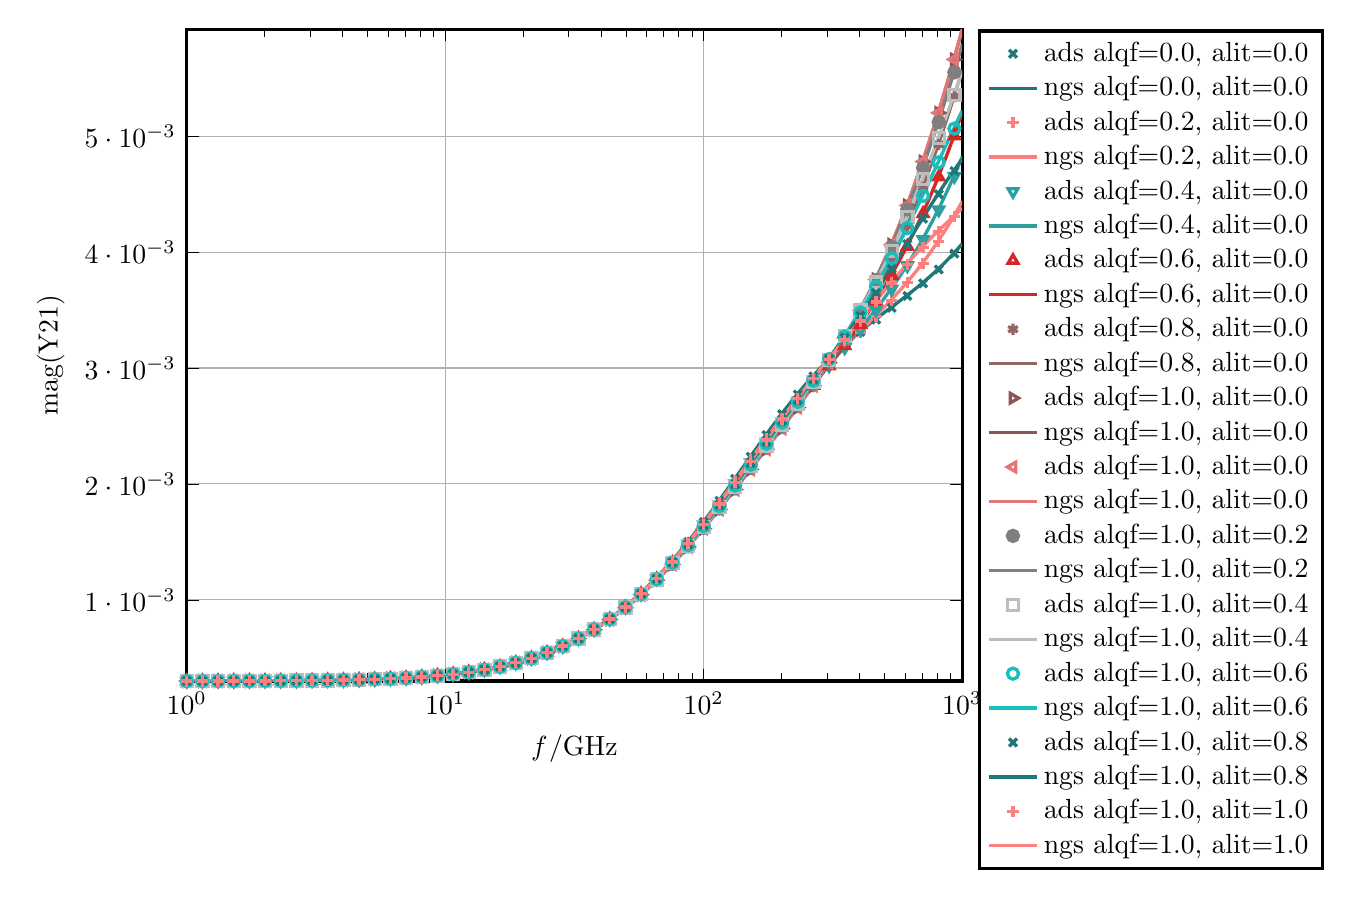
\begin{tikzpicture}[font=\normalsize]
\pgfplotsset{every axis/.append style={very thick}},
\definecolor{color0}{rgb}{0.12157, 0.46667, 0.46667}
\definecolor{color1}{rgb}{1.00000, 0.49804, 0.49804}
\definecolor{color2}{rgb}{0.17255, 0.62745, 0.62745}
\definecolor{color3}{rgb}{0.83922, 0.15294, 0.15294}
\definecolor{color4}{rgb}{0.58039, 0.40392, 0.40392}
\definecolor{color5}{rgb}{0.54902, 0.33725, 0.33725}
\definecolor{color6}{rgb}{0.89020, 0.46667, 0.46667}
\definecolor{color7}{rgb}{0.49804, 0.49804, 0.49804}
\definecolor{color8}{rgb}{0.73725, 0.74118, 0.74118}
\definecolor{color9}{rgb}{0.09020, 0.74510, 0.74510}

\begin{axis}[
width=4.5in,
xlabel={$f_{\mathrm{}}^{}/\si{\giga\hertz}$},
ylabel={mag(Y21)},
xmode=log,
% xmin=0,
% xmax=0,
% restrict x to domain=0:1,
log basis x=10,
% ymin=0,
% ymax=0,
% restrict y to domain=0:1,
log basis y=10,
xmajorgrids,
enlargelimits=false,
scaled ticks=false,
ymajorgrids,
x tick style={color=black},
y tick style={color=black},
x grid style={white!69.01960784313725!black},
y grid style={white!69.01960784313725!black},
/tikz/mark repeat=2,
legend style={at={(1.02,1.00)}, anchor=north west,legend cell align=left, align=left},
]
\addplot [color=color0, only marks, mark=x, mark options={solid}, mark phase=0, ]
  table[row sep=crcr, x expr=\thisrowno{0}*1.000000e-09, y expr=\thisrowno{1}*1.000000e+00]{
1e+09 0.000299058\\
1.07227e+09 0.000299143\\
1.14976e+09 0.000299242\\
1.23285e+09 0.000299355\\
1.32194e+09 0.000299484\\
1.41747e+09 0.000299633\\
1.51991e+09 0.000299805\\
1.62975e+09 0.000300002\\
1.74753e+09 0.000300228\\
1.87382e+09 0.000300488\\
2.00923e+09 0.000300787\\
2.15443e+09 0.00030113\\
2.31013e+09 0.000301525\\
2.47708e+09 0.000301977\\
2.65609e+09 0.000302497\\
2.84804e+09 0.000303094\\
3.05386e+09 0.000303779\\
3.27455e+09 0.000304565\\
3.51119e+09 0.000305466\\
3.76494e+09 0.000306498\\
4.03702e+09 0.000307682\\
4.32876e+09 0.000309037\\
4.64159e+09 0.000310588\\
4.97702e+09 0.000312361\\
5.3367e+09 0.000314388\\
5.72237e+09 0.000316702\\
6.13591e+09 0.000319342\\
6.57933e+09 0.00032235\\
7.0548e+09 0.000325773\\
7.56463e+09 0.000329664\\
8.11131e+09 0.000334079\\
8.69749e+09 0.000339083\\
9.32603e+09 0.000344743\\
1e+10 0.000351135\\
1.07227e+10 0.000358337\\
1.14976e+10 0.000366437\\
1.23285e+10 0.000375525\\
1.32194e+10 0.000385698\\
1.41747e+10 0.000397058\\
1.51991e+10 0.000409711\\
1.62975e+10 0.000423769\\
1.74753e+10 0.000439346\\
1.87382e+10 0.000456562\\
2.00923e+10 0.000475536\\
2.15443e+10 0.000496396\\
2.31013e+10 0.000519268\\
2.47708e+10 0.000544281\\
2.65609e+10 0.000571568\\
2.84804e+10 0.000601262\\
3.05386e+10 0.000633497\\
3.27455e+10 0.000668407\\
3.51119e+10 0.000706128\\
3.76494e+10 0.00074679\\
4.03702e+10 0.000790524\\
4.32876e+10 0.000837451\\
4.64159e+10 0.000887688\\
4.97702e+10 0.00094134\\
5.3367e+10 0.000998495\\
5.72237e+10 0.00105923\\
6.13591e+10 0.00112358\\
6.57933e+10 0.00119157\\
7.0548e+10 0.00126319\\
7.56463e+10 0.00133837\\
8.11131e+10 0.00141701\\
8.69749e+10 0.00149894\\
9.32603e+10 0.00158396\\
1e+11 0.00167178\\
1.07227e+11 0.00176207\\
1.14976e+11 0.0018544\\
1.23285e+11 0.00194832\\
1.32194e+11 0.00204331\\
1.41747e+11 0.0021388\\
1.51991e+11 0.0022342\\
1.62975e+11 0.00232892\\
1.74753e+11 0.00242235\\
1.87382e+11 0.00251392\\
2.00923e+11 0.00260313\\
2.15443e+11 0.00268951\\
2.31013e+11 0.00277269\\
2.47708e+11 0.0028524\\
2.65609e+11 0.00292845\\
2.84804e+11 0.00300077\\
3.05386e+11 0.00306941\\
3.27455e+11 0.00313449\\
3.51119e+11 0.00319624\\
3.76494e+11 0.00325498\\
4.03702e+11 0.00331109\\
4.32876e+11 0.00336503\\
4.64159e+11 0.00341731\\
4.97702e+11 0.00346848\\
5.3367e+11 0.00351916\\
5.72237e+11 0.00356997\\
6.13591e+11 0.00362157\\
6.57933e+11 0.00367465\\
7.0548e+11 0.00372992\\
7.56463e+11 0.00378808\\
8.11131e+11 0.00384987\\
8.69749e+11 0.00391599\\
9.32603e+11 0.00398715\\
1e+12 0.00406403\\
};
\addlegendentry{ads alqf=0.0, alit=0.0}
\addplot [color=color0, solid,  mark phase=0, ]
  table[row sep=crcr, x expr=\thisrowno{0}*1.000000e-09, y expr=\thisrowno{1}*1.000000e+00]{
1e+09 0.00029906\\
1.02306e+09 0.000299087\\
1.04665e+09 0.000299115\\
1.07079e+09 0.000299144\\
1.09548e+09 0.000299175\\
1.12074e+09 0.000299207\\
1.14658e+09 0.000299241\\
1.17302e+09 0.000299276\\
1.20007e+09 0.000299312\\
1.22775e+09 0.000299351\\
1.25606e+09 0.000299391\\
1.28502e+09 0.000299433\\
1.31466e+09 0.000299477\\
1.34497e+09 0.000299524\\
1.37599e+09 0.000299572\\
1.40772e+09 0.000299622\\
1.44018e+09 0.000299675\\
1.47339e+09 0.000299731\\
1.50736e+09 0.000299789\\
1.54212e+09 0.000299849\\
1.57768e+09 0.000299913\\
1.61406e+09 0.000299979\\
1.65128e+09 0.000300049\\
1.68936e+09 0.000300121\\
1.72832e+09 0.000300197\\
1.76817e+09 0.000300277\\
1.80895e+09 0.00030036\\
1.85066e+09 0.000300448\\
1.89334e+09 0.000300539\\
1.937e+09 0.000300634\\
1.98166e+09 0.000300734\\
2.02736e+09 0.000300839\\
2.07411e+09 0.000300948\\
2.12194e+09 0.000301063\\
2.17087e+09 0.000301182\\
2.22093e+09 0.000301308\\
2.27214e+09 0.000301439\\
2.32454e+09 0.000301576\\
2.37814e+09 0.000301719\\
2.43298e+09 0.000301869\\
2.48908e+09 0.000302027\\
2.54648e+09 0.000302191\\
2.6052e+09 0.000302363\\
2.66528e+09 0.000302543\\
2.72674e+09 0.000302731\\
2.78962e+09 0.000302927\\
2.85394e+09 0.000303133\\
2.91976e+09 0.000303349\\
2.98708e+09 0.000303574\\
3.05597e+09 0.000303809\\
3.12644e+09 0.000304056\\
3.19853e+09 0.000304313\\
3.27229e+09 0.000304583\\
3.34775e+09 0.000304864\\
3.42494e+09 0.000305159\\
3.50392e+09 0.000305467\\
3.58472e+09 0.000305789\\
3.66738e+09 0.000306126\\
3.75195e+09 0.000306478\\
3.83847e+09 0.000306847\\
3.92699e+09 0.000307232\\
4.01754e+09 0.000307634\\
4.11019e+09 0.000308054\\
4.20496e+09 0.000308494\\
4.30193e+09 0.000308954\\
4.40113e+09 0.000309434\\
4.50262e+09 0.000309936\\
4.60645e+09 0.00031046\\
4.71267e+09 0.000311008\\
4.82135e+09 0.00031158\\
4.93253e+09 0.000312178\\
5.04627e+09 0.000312803\\
5.16263e+09 0.000313455\\
5.28168e+09 0.000314137\\
5.40348e+09 0.000314848\\
5.52808e+09 0.000315591\\
5.65556e+09 0.000316367\\
5.78597e+09 0.000317177\\
5.91939e+09 0.000318023\\
6.05589e+09 0.000318905\\
6.19554e+09 0.000319826\\
6.33841e+09 0.000320787\\
6.48457e+09 0.00032179\\
6.6341e+09 0.000322836\\
6.78708e+09 0.000323928\\
6.94359e+09 0.000325066\\
7.10371e+09 0.000326253\\
7.26752e+09 0.00032749\\
7.43511e+09 0.00032878\\
7.60656e+09 0.000330125\\
7.78196e+09 0.000331527\\
7.96141e+09 0.000332987\\
8.145e+09 0.000334509\\
8.33282e+09 0.000336094\\
8.52497e+09 0.000337744\\
8.72156e+09 0.000339463\\
8.92267e+09 0.000341252\\
9.12843e+09 0.000343115\\
9.33893e+09 0.000345053\\
9.55428e+09 0.000347069\\
9.7746e+09 0.000349167\\
1e+10 0.000351349\\
1.02306e+10 0.000353617\\
1.04665e+10 0.000355976\\
1.07079e+10 0.000358427\\
1.09548e+10 0.000360974\\
1.12074e+10 0.00036362\\
1.14658e+10 0.000366368\\
1.17302e+10 0.000369221\\
1.20007e+10 0.000372183\\
1.22775e+10 0.000375257\\
1.25606e+10 0.000378447\\
1.28502e+10 0.000381756\\
1.31466e+10 0.000385187\\
1.34497e+10 0.000388744\\
1.37599e+10 0.000392432\\
1.40772e+10 0.000396252\\
1.44018e+10 0.00040021\\
1.47339e+10 0.00040431\\
1.50736e+10 0.000408554\\
1.54212e+10 0.000412947\\
1.57768e+10 0.000417492\\
1.61406e+10 0.000422195\\
1.65128e+10 0.000427058\\
1.68936e+10 0.000432087\\
1.72832e+10 0.000437284\\
1.76817e+10 0.000442655\\
1.80895e+10 0.000448203\\
1.85066e+10 0.000453932\\
1.89334e+10 0.000459848\\
1.937e+10 0.000465954\\
1.98166e+10 0.000472254\\
2.02736e+10 0.000478754\\
2.07411e+10 0.000485457\\
2.12194e+10 0.000492367\\
2.17087e+10 0.00049949\\
2.22093e+10 0.00050683\\
2.27214e+10 0.000514391\\
2.32454e+10 0.000522178\\
2.37814e+10 0.000530195\\
2.43298e+10 0.000538447\\
2.48908e+10 0.000546938\\
2.54648e+10 0.000555674\\
2.6052e+10 0.000564659\\
2.66528e+10 0.000573897\\
2.72674e+10 0.000583393\\
2.78962e+10 0.000593153\\
2.85394e+10 0.000603179\\
2.91976e+10 0.000613478\\
2.98708e+10 0.000624054\\
3.05597e+10 0.000634912\\
3.12644e+10 0.000646056\\
3.19853e+10 0.000657491\\
3.27229e+10 0.000669222\\
3.34775e+10 0.000681253\\
3.42494e+10 0.00069359\\
3.50392e+10 0.000706236\\
3.58472e+10 0.000719196\\
3.66738e+10 0.000732475\\
3.75195e+10 0.000746078\\
3.83847e+10 0.000760008\\
3.92699e+10 0.000774271\\
4.01754e+10 0.000788871\\
4.11019e+10 0.000803811\\
4.20496e+10 0.000819096\\
4.30193e+10 0.00083473\\
4.40113e+10 0.000850718\\
4.50262e+10 0.000867062\\
4.60645e+10 0.000883767\\
4.71267e+10 0.000900836\\
4.82135e+10 0.000918272\\
4.93253e+10 0.00093608\\
5.04627e+10 0.000954261\\
5.16263e+10 0.000972819\\
5.28168e+10 0.000991756\\
5.40348e+10 0.00101107\\
5.52808e+10 0.00103078\\
5.65556e+10 0.00105087\\
5.78597e+10 0.00107134\\
5.91939e+10 0.0010922\\
6.05589e+10 0.00111346\\
6.19554e+10 0.0011351\\
6.33841e+10 0.00115713\\
6.48457e+10 0.00117955\\
6.6341e+10 0.00120236\\
6.78708e+10 0.00122556\\
6.94359e+10 0.00124914\\
7.10371e+10 0.0012731\\
7.26752e+10 0.00129745\\
7.43511e+10 0.00132217\\
7.60656e+10 0.00134727\\
7.78196e+10 0.00137274\\
7.96141e+10 0.00139857\\
8.145e+10 0.00142476\\
8.33282e+10 0.0014513\\
8.52497e+10 0.00147819\\
8.72156e+10 0.00150541\\
8.92267e+10 0.00153297\\
9.12843e+10 0.00156084\\
9.33893e+10 0.00158902\\
9.55428e+10 0.00161751\\
9.7746e+10 0.00164628\\
1e+11 0.00167533\\
1.02306e+11 0.00170464\\
1.04665e+11 0.0017342\\
1.07079e+11 0.001764\\
1.09548e+11 0.00179401\\
1.12074e+11 0.00182424\\
1.14658e+11 0.00185465\\
1.17302e+11 0.00188524\\
1.20007e+11 0.00191597\\
1.22775e+11 0.00194685\\
1.25606e+11 0.00197784\\
1.28502e+11 0.00200894\\
1.31466e+11 0.00204011\\
1.34497e+11 0.00207134\\
1.37599e+11 0.00210261\\
1.40772e+11 0.00213389\\
1.44018e+11 0.00216518\\
1.47339e+11 0.00219644\\
1.50736e+11 0.00222765\\
1.54212e+11 0.0022588\\
1.57768e+11 0.00228987\\
1.61406e+11 0.00232082\\
1.65128e+11 0.00235164\\
1.68936e+11 0.00238232\\
1.72832e+11 0.00241283\\
1.76817e+11 0.00244314\\
1.80895e+11 0.00247325\\
1.85066e+11 0.00250313\\
1.89334e+11 0.00253277\\
1.937e+11 0.00256214\\
1.98166e+11 0.00259124\\
2.02736e+11 0.00262004\\
2.07411e+11 0.00264854\\
2.12194e+11 0.00267671\\
2.17087e+11 0.00270454\\
2.22093e+11 0.00273203\\
2.27214e+11 0.00275917\\
2.32454e+11 0.00278593\\
2.37814e+11 0.00281232\\
2.43298e+11 0.00283833\\
2.48908e+11 0.00286395\\
2.54648e+11 0.00288918\\
2.6052e+11 0.00291401\\
2.66528e+11 0.00293845\\
2.72674e+11 0.00296248\\
2.78962e+11 0.00298612\\
2.85394e+11 0.00300935\\
2.91976e+11 0.0030322\\
2.98708e+11 0.00305465\\
3.05597e+11 0.00307671\\
3.12644e+11 0.0030984\\
3.19853e+11 0.0031197\\
3.27229e+11 0.00314065\\
3.34775e+11 0.00316124\\
3.42494e+11 0.00318148\\
3.50392e+11 0.00320138\\
3.58472e+11 0.00322096\\
3.66738e+11 0.00324023\\
3.75195e+11 0.0032592\\
3.83847e+11 0.00327789\\
3.92699e+11 0.00329631\\
4.01754e+11 0.00331447\\
4.11019e+11 0.00333241\\
4.20496e+11 0.00335012\\
4.30193e+11 0.00336763\\
4.40113e+11 0.00338495\\
4.50262e+11 0.00340212\\
4.60645e+11 0.00341914\\
4.71267e+11 0.00343603\\
4.82135e+11 0.00345282\\
4.93253e+11 0.00346953\\
5.04627e+11 0.00348617\\
5.16263e+11 0.00350278\\
5.28168e+11 0.00351936\\
5.40348e+11 0.00353595\\
5.52808e+11 0.00355257\\
5.65556e+11 0.00356923\\
5.78597e+11 0.00358597\\
5.91939e+11 0.00360281\\
6.05589e+11 0.00361976\\
6.19554e+11 0.00363686\\
6.33841e+11 0.00365413\\
6.48457e+11 0.00367159\\
6.6341e+11 0.00368927\\
6.78708e+11 0.0037072\\
6.94359e+11 0.00372539\\
7.10371e+11 0.00374387\\
7.26752e+11 0.00376268\\
7.43511e+11 0.00378182\\
7.60656e+11 0.00380134\\
7.78196e+11 0.00382125\\
7.96141e+11 0.00384157\\
8.145e+11 0.00386234\\
8.33282e+11 0.00388358\\
8.52497e+11 0.00390532\\
8.72156e+11 0.00392757\\
8.92267e+11 0.00395036\\
9.12843e+11 0.00397373\\
9.33893e+11 0.00399768\\
9.55428e+11 0.00402224\\
9.7746e+11 0.00404744\\
1e+12 0.0040733\\
};
\addlegendentry{ngs alqf=0.0, alit=0.0}
\addplot [color=color1, only marks, mark=+, mark options={solid}, mark phase=0, ]
  table[row sep=crcr, x expr=\thisrowno{0}*1.000000e-09, y expr=\thisrowno{1}*1.000000e+00]{
1e+09 0.000299058\\
1.07227e+09 0.000299143\\
1.14976e+09 0.000299241\\
1.23285e+09 0.000299354\\
1.32194e+09 0.000299484\\
1.41747e+09 0.000299633\\
1.51991e+09 0.000299804\\
1.62975e+09 0.000300001\\
1.74753e+09 0.000300228\\
1.87382e+09 0.000300488\\
2.00923e+09 0.000300786\\
2.15443e+09 0.000301129\\
2.31013e+09 0.000301524\\
2.47708e+09 0.000301976\\
2.65609e+09 0.000302496\\
2.84804e+09 0.000303093\\
3.05386e+09 0.000303777\\
3.27455e+09 0.000304563\\
3.51119e+09 0.000305463\\
3.76494e+09 0.000306496\\
4.03702e+09 0.000307679\\
4.32876e+09 0.000309033\\
4.64159e+09 0.000310583\\
4.97702e+09 0.000312356\\
5.3367e+09 0.000314382\\
5.72237e+09 0.000316695\\
6.13591e+09 0.000319334\\
6.57933e+09 0.00032234\\
7.0548e+09 0.000325762\\
7.56463e+09 0.00032965\\
8.11131e+09 0.000334064\\
8.69749e+09 0.000339065\\
9.32603e+09 0.000344722\\
1e+10 0.000351109\\
1.07227e+10 0.000358306\\
1.14976e+10 0.0003664\\
1.23285e+10 0.00037548\\
1.32194e+10 0.000385644\\
1.41747e+10 0.000396993\\
1.51991e+10 0.000409633\\
1.62975e+10 0.000423674\\
1.74753e+10 0.000439231\\
1.87382e+10 0.000456421\\
2.00923e+10 0.000475366\\
2.15443e+10 0.000496188\\
2.31013e+10 0.000519015\\
2.47708e+10 0.000543972\\
2.65609e+10 0.000571191\\
2.84804e+10 0.000600802\\
3.05386e+10 0.000632935\\
3.27455e+10 0.000667722\\
3.51119e+10 0.000705292\\
3.76494e+10 0.000745772\\
4.03702e+10 0.000789283\\
4.32876e+10 0.000835943\\
4.64159e+10 0.000885856\\
4.97702e+10 0.000939118\\
5.3367e+10 0.000995807\\
5.72237e+10 0.00105598\\
6.13591e+10 0.00111967\\
6.57933e+10 0.00118688\\
7.0548e+10 0.00125757\\
7.56463e+10 0.00133167\\
8.11131e+10 0.00140905\\
8.69749e+10 0.00148955\\
9.32603e+10 0.00157293\\
1e+11 0.00165889\\
1.07227e+11 0.00174711\\
1.14976e+11 0.00183716\\
1.23285e+11 0.00192861\\
1.32194e+11 0.00202097\\
1.41747e+11 0.00211371\\
1.51991e+11 0.00220632\\
1.62975e+11 0.00229827\\
1.74753e+11 0.00238905\\
1.87382e+11 0.00247824\\
2.00923e+11 0.00256543\\
2.15443e+11 0.00265033\\
2.31013e+11 0.00273271\\
2.47708e+11 0.00281248\\
2.65609e+11 0.00288963\\
2.84804e+11 0.00296427\\
3.05386e+11 0.0030366\\
3.27455e+11 0.00310694\\
3.51119e+11 0.00317567\\
3.76494e+11 0.00324328\\
4.03702e+11 0.0033103\\
4.32876e+11 0.00337733\\
4.64159e+11 0.00344501\\
4.97702e+11 0.00351401\\
5.3367e+11 0.00358501\\
5.72237e+11 0.00365873\\
6.13591e+11 0.00373587\\
6.57933e+11 0.00381714\\
7.0548e+11 0.00390322\\
7.56463e+11 0.00399478\\
8.11131e+11 0.00409245\\
8.69749e+11 0.00419685\\
9.32603e+11 0.00430852\\
1e+12 0.00442795\\
};
\addlegendentry{ads alqf=0.2, alit=0.0}
\addplot [color=color1, solid,  mark phase=0, ]
  table[row sep=crcr, x expr=\thisrowno{0}*1.000000e-09, y expr=\thisrowno{1}*1.000000e+00]{
1e+09 0.00029906\\
1.02306e+09 0.000299087\\
1.04665e+09 0.000299115\\
1.07079e+09 0.000299144\\
1.09548e+09 0.000299175\\
1.12074e+09 0.000299207\\
1.14658e+09 0.00029924\\
1.17302e+09 0.000299275\\
1.20007e+09 0.000299312\\
1.22775e+09 0.000299351\\
1.25606e+09 0.000299391\\
1.28502e+09 0.000299433\\
1.31466e+09 0.000299477\\
1.34497e+09 0.000299523\\
1.37599e+09 0.000299572\\
1.40772e+09 0.000299622\\
1.44018e+09 0.000299675\\
1.47339e+09 0.00029973\\
1.50736e+09 0.000299788\\
1.54212e+09 0.000299849\\
1.57768e+09 0.000299912\\
1.61406e+09 0.000299979\\
1.65128e+09 0.000300048\\
1.68936e+09 0.000300121\\
1.72832e+09 0.000300197\\
1.76817e+09 0.000300276\\
1.80895e+09 0.00030036\\
1.85066e+09 0.000300447\\
1.89334e+09 0.000300538\\
1.937e+09 0.000300634\\
1.98166e+09 0.000300733\\
2.02736e+09 0.000300838\\
2.07411e+09 0.000300947\\
2.12194e+09 0.000301062\\
2.17087e+09 0.000301181\\
2.22093e+09 0.000301307\\
2.27214e+09 0.000301438\\
2.32454e+09 0.000301575\\
2.37814e+09 0.000301718\\
2.43298e+09 0.000301868\\
2.48908e+09 0.000302025\\
2.54648e+09 0.00030219\\
2.6052e+09 0.000302361\\
2.66528e+09 0.000302541\\
2.72674e+09 0.000302729\\
2.78962e+09 0.000302926\\
2.85394e+09 0.000303132\\
2.91976e+09 0.000303347\\
2.98708e+09 0.000303572\\
3.05597e+09 0.000303807\\
3.12644e+09 0.000304054\\
3.19853e+09 0.000304311\\
3.27229e+09 0.000304581\\
3.34775e+09 0.000304862\\
3.42494e+09 0.000305157\\
3.50392e+09 0.000305465\\
3.58472e+09 0.000305787\\
3.66738e+09 0.000306124\\
3.75195e+09 0.000306476\\
3.83847e+09 0.000306844\\
3.92699e+09 0.000307228\\
4.01754e+09 0.000307631\\
4.11019e+09 0.000308051\\
4.20496e+09 0.000308491\\
4.30193e+09 0.00030895\\
4.40113e+09 0.00030943\\
4.50262e+09 0.000309931\\
4.60645e+09 0.000310456\\
4.71267e+09 0.000311003\\
4.82135e+09 0.000311575\\
4.93253e+09 0.000312173\\
5.04627e+09 0.000312798\\
5.16263e+09 0.00031345\\
5.28168e+09 0.000314131\\
5.40348e+09 0.000314842\\
5.52808e+09 0.000315585\\
5.65556e+09 0.00031636\\
5.78597e+09 0.00031717\\
5.91939e+09 0.000318015\\
6.05589e+09 0.000318897\\
6.19554e+09 0.000319818\\
6.33841e+09 0.000320779\\
6.48457e+09 0.000321781\\
6.6341e+09 0.000322827\\
6.78708e+09 0.000323917\\
6.94359e+09 0.000325055\\
7.10371e+09 0.000326241\\
7.26752e+09 0.000327478\\
7.43511e+09 0.000328768\\
7.60656e+09 0.000330112\\
7.78196e+09 0.000331513\\
7.96141e+09 0.000332972\\
8.145e+09 0.000334493\\
8.33282e+09 0.000336077\\
8.52497e+09 0.000337726\\
8.72156e+09 0.000339444\\
8.92267e+09 0.000341232\\
9.12843e+09 0.000343094\\
9.33893e+09 0.000345031\\
9.55428e+09 0.000347046\\
9.7746e+09 0.000349142\\
1e+10 0.000351323\\
1.02306e+10 0.00035359\\
1.04665e+10 0.000355946\\
1.07079e+10 0.000358396\\
1.09548e+10 0.000360941\\
1.12074e+10 0.000363585\\
1.14658e+10 0.00036633\\
1.17302e+10 0.000369182\\
1.20007e+10 0.000372141\\
1.22775e+10 0.000375213\\
1.25606e+10 0.0003784\\
1.28502e+10 0.000381706\\
1.31466e+10 0.000385134\\
1.34497e+10 0.000388688\\
1.37599e+10 0.000392372\\
1.40772e+10 0.000396188\\
1.44018e+10 0.000400142\\
1.47339e+10 0.000404237\\
1.50736e+10 0.000408477\\
1.54212e+10 0.000412865\\
1.57768e+10 0.000417405\\
1.61406e+10 0.000422102\\
1.65128e+10 0.000426959\\
1.68936e+10 0.000431981\\
1.72832e+10 0.000437172\\
1.76817e+10 0.000442535\\
1.80895e+10 0.000448075\\
1.85066e+10 0.000453797\\
1.89334e+10 0.000459703\\
1.937e+10 0.0004658\\
1.98166e+10 0.00047209\\
2.02736e+10 0.000478578\\
2.07411e+10 0.00048527\\
2.12194e+10 0.000492168\\
2.17087e+10 0.000499277\\
2.22093e+10 0.000506603\\
2.27214e+10 0.000514149\\
2.32454e+10 0.000521919\\
2.37814e+10 0.000529919\\
2.43298e+10 0.000538152\\
2.48908e+10 0.000546624\\
2.54648e+10 0.000555339\\
2.6052e+10 0.000564301\\
2.66528e+10 0.000573515\\
2.72674e+10 0.000582986\\
2.78962e+10 0.000592718\\
2.85394e+10 0.000602715\\
2.91976e+10 0.000612983\\
2.98708e+10 0.000623526\\
3.05597e+10 0.000634348\\
3.12644e+10 0.000645454\\
3.19853e+10 0.000656849\\
3.27229e+10 0.000668536\\
3.34775e+10 0.000680522\\
3.42494e+10 0.000692809\\
3.50392e+10 0.000705403\\
3.58472e+10 0.000718307\\
3.66738e+10 0.000731527\\
3.75195e+10 0.000745067\\
3.83847e+10 0.00075893\\
3.92699e+10 0.000773121\\
4.01754e+10 0.000787644\\
4.11019e+10 0.000802503\\
4.20496e+10 0.000817702\\
4.30193e+10 0.000833244\\
4.40113e+10 0.000849134\\
4.50262e+10 0.000865374\\
4.60645e+10 0.000881968\\
4.71267e+10 0.00089892\\
4.82135e+10 0.000916232\\
4.93253e+10 0.000933907\\
5.04627e+10 0.000951948\\
5.16263e+10 0.000970357\\
5.28168e+10 0.000989136\\
5.40348e+10 0.00100829\\
5.52808e+10 0.00102781\\
5.65556e+10 0.00104771\\
5.78597e+10 0.00106799\\
5.91939e+10 0.00108864\\
6.05589e+10 0.00110967\\
6.19554e+10 0.00113108\\
6.33841e+10 0.00115286\\
6.48457e+10 0.00117502\\
6.6341e+10 0.00119755\\
6.78708e+10 0.00122046\\
6.94359e+10 0.00124373\\
7.10371e+10 0.00126737\\
7.26752e+10 0.00129138\\
7.43511e+10 0.00131574\\
7.60656e+10 0.00134047\\
7.78196e+10 0.00136554\\
7.96141e+10 0.00139096\\
8.145e+10 0.00141671\\
8.33282e+10 0.0014428\\
8.52497e+10 0.00146921\\
8.72156e+10 0.00149594\\
8.92267e+10 0.00152298\\
9.12843e+10 0.00155031\\
9.33893e+10 0.00157793\\
9.55428e+10 0.00160583\\
9.7746e+10 0.00163399\\
1e+11 0.00166241\\
1.02306e+11 0.00169107\\
1.04665e+11 0.00171995\\
1.07079e+11 0.00174905\\
1.09548e+11 0.00177835\\
1.12074e+11 0.00180783\\
1.14658e+11 0.00183747\\
1.17302e+11 0.00186727\\
1.20007e+11 0.00189721\\
1.22775e+11 0.00192726\\
1.25606e+11 0.00195741\\
1.28502e+11 0.00198764\\
1.31466e+11 0.00201794\\
1.34497e+11 0.00204829\\
1.37599e+11 0.00207866\\
1.40772e+11 0.00210904\\
1.44018e+11 0.00213941\\
1.47339e+11 0.00216976\\
1.50736e+11 0.00220006\\
1.54212e+11 0.00223029\\
1.57768e+11 0.00226044\\
1.61406e+11 0.0022905\\
1.65128e+11 0.00232043\\
1.68936e+11 0.00235023\\
1.72832e+11 0.00237988\\
1.76817e+11 0.00240937\\
1.80895e+11 0.00243868\\
1.85066e+11 0.00246779\\
1.89334e+11 0.0024967\\
1.937e+11 0.00252539\\
1.98166e+11 0.00255384\\
2.02736e+11 0.00258206\\
2.07411e+11 0.00261003\\
2.12194e+11 0.00263773\\
2.17087e+11 0.00266518\\
2.22093e+11 0.00269235\\
2.27214e+11 0.00271925\\
2.32454e+11 0.00274587\\
2.37814e+11 0.0027722\\
2.43298e+11 0.00279826\\
2.48908e+11 0.00282403\\
2.54648e+11 0.00284952\\
2.6052e+11 0.00287474\\
2.66528e+11 0.00289968\\
2.72674e+11 0.00292435\\
2.78962e+11 0.00294876\\
2.85394e+11 0.00297291\\
2.91976e+11 0.00299682\\
2.98708e+11 0.00302049\\
3.05597e+11 0.00304394\\
3.12644e+11 0.00306717\\
3.19853e+11 0.0030902\\
3.27229e+11 0.00311304\\
3.34775e+11 0.00313572\\
3.42494e+11 0.00315823\\
3.50392e+11 0.00318061\\
3.58472e+11 0.00320286\\
3.66738e+11 0.00322501\\
3.75195e+11 0.00324708\\
3.83847e+11 0.00326907\\
3.92699e+11 0.00329103\\
4.01754e+11 0.00331295\\
4.11019e+11 0.00333488\\
4.20496e+11 0.00335682\\
4.30193e+11 0.0033788\\
4.40113e+11 0.00340085\\
4.50262e+11 0.00342298\\
4.60645e+11 0.00344522\\
4.71267e+11 0.00346759\\
4.82135e+11 0.00349012\\
4.93253e+11 0.00351284\\
5.04627e+11 0.00353575\\
5.16263e+11 0.0035589\\
5.28168e+11 0.00358231\\
5.40348e+11 0.00360599\\
5.52808e+11 0.00362998\\
5.65556e+11 0.00365429\\
5.78597e+11 0.00367896\\
5.91939e+11 0.00370401\\
6.05589e+11 0.00372946\\
6.19554e+11 0.00375534\\
6.33841e+11 0.00378167\\
6.48457e+11 0.00380848\\
6.6341e+11 0.00383578\\
6.78708e+11 0.00386362\\
6.94359e+11 0.003892\\
7.10371e+11 0.00392095\\
7.26752e+11 0.00395049\\
7.43511e+11 0.00398065\\
7.60656e+11 0.00401145\\
7.78196e+11 0.00404291\\
7.96141e+11 0.00407505\\
8.145e+11 0.00410789\\
8.33282e+11 0.00414146\\
8.52497e+11 0.00417577\\
8.72156e+11 0.00421084\\
8.92267e+11 0.00424669\\
9.12843e+11 0.00428334\\
9.33893e+11 0.00432081\\
9.55428e+11 0.00435911\\
9.7746e+11 0.00439826\\
1e+12 0.00443827\\
};
\addlegendentry{ngs alqf=0.2, alit=0.0}
\addplot [color=color2, only marks, mark=triangle, mark options={solid, rotate=180}, mark phase=0, ]
  table[row sep=crcr, x expr=\thisrowno{0}*1.000000e-09, y expr=\thisrowno{1}*1.000000e+00]{
1e+09 0.000299058\\
1.07227e+09 0.000299143\\
1.14976e+09 0.000299241\\
1.23285e+09 0.000299354\\
1.32194e+09 0.000299484\\
1.41747e+09 0.000299633\\
1.51991e+09 0.000299804\\
1.62975e+09 0.000300001\\
1.74753e+09 0.000300227\\
1.87382e+09 0.000300487\\
2.00923e+09 0.000300786\\
2.15443e+09 0.000301129\\
2.31013e+09 0.000301523\\
2.47708e+09 0.000301975\\
2.65609e+09 0.000302495\\
2.84804e+09 0.000303091\\
3.05386e+09 0.000303775\\
3.27455e+09 0.000304561\\
3.51119e+09 0.000305461\\
3.76494e+09 0.000306493\\
4.03702e+09 0.000307675\\
4.32876e+09 0.000309029\\
4.64159e+09 0.000310579\\
4.97702e+09 0.000312351\\
5.3367e+09 0.000314376\\
5.72237e+09 0.000316689\\
6.13591e+09 0.000319326\\
6.57933e+09 0.000322331\\
7.0548e+09 0.000325751\\
7.56463e+09 0.000329637\\
8.11131e+09 0.000334048\\
8.69749e+09 0.000339046\\
9.32603e+09 0.0003447\\
1e+10 0.000351083\\
1.07227e+10 0.000358275\\
1.14976e+10 0.000366362\\
1.23285e+10 0.000375435\\
1.32194e+10 0.00038559\\
1.41747e+10 0.000396928\\
1.51991e+10 0.000409554\\
1.62975e+10 0.000423579\\
1.74753e+10 0.000439116\\
1.87382e+10 0.000456281\\
2.00923e+10 0.000475196\\
2.15443e+10 0.000495981\\
2.31013e+10 0.000518762\\
2.47708e+10 0.000543664\\
2.65609e+10 0.000570815\\
2.84804e+10 0.000600343\\
3.05386e+10 0.000632376\\
3.27455e+10 0.00066704\\
3.51119e+10 0.000704461\\
3.76494e+10 0.00074476\\
4.03702e+10 0.000788052\\
4.32876e+10 0.000834447\\
4.64159e+10 0.000884043\\
4.97702e+10 0.000936924\\
5.3367e+10 0.000993157\\
5.72237e+10 0.00105279\\
6.13591e+10 0.00111584\\
6.57933e+10 0.00118229\\
7.0548e+10 0.0012521\\
7.56463e+10 0.00132518\\
8.11131e+10 0.00140139\\
8.69749e+10 0.00148054\\
9.32603e+10 0.0015624\\
1e+11 0.00164668\\
1.07227e+11 0.00173304\\
1.14976e+11 0.0018211\\
1.23285e+11 0.00191043\\
1.32194e+11 0.00200058\\
1.41747e+11 0.00209111\\
1.51991e+11 0.00218155\\
1.62975e+11 0.00227147\\
1.74753e+11 0.0023605\\
1.87382e+11 0.0024483\\
2.00923e+11 0.00253463\\
2.15443e+11 0.00261933\\
2.31013e+11 0.00270236\\
2.47708e+11 0.00278376\\
2.65609e+11 0.0028637\\
2.84804e+11 0.00294245\\
3.05386e+11 0.00302037\\
3.27455e+11 0.00309793\\
3.51119e+11 0.00317565\\
3.76494e+11 0.00325415\\
4.03702e+11 0.00333408\\
4.32876e+11 0.00341612\\
4.64159e+11 0.00350098\\
4.97702e+11 0.0035894\\
5.3367e+11 0.0036821\\
5.72237e+11 0.00377976\\
6.13591e+11 0.00388308\\
6.57933e+11 0.00399268\\
7.0548e+11 0.00410917\\
7.56463e+11 0.0042331\\
8.11131e+11 0.00436494\\
8.69749e+11 0.00450513\\
9.32603e+11 0.00465402\\
1e+12 0.0048119\\
};
\addlegendentry{ads alqf=0.4, alit=0.0}
\addplot [color=color2, solid,  mark phase=0, ]
  table[row sep=crcr, x expr=\thisrowno{0}*1.000000e-09, y expr=\thisrowno{1}*1.000000e+00]{
1e+09 0.00029906\\
1.02306e+09 0.000299087\\
1.04665e+09 0.000299115\\
1.07079e+09 0.000299144\\
1.09548e+09 0.000299174\\
1.12074e+09 0.000299207\\
1.14658e+09 0.00029924\\
1.17302e+09 0.000299275\\
1.20007e+09 0.000299312\\
1.22775e+09 0.00029935\\
1.25606e+09 0.000299391\\
1.28502e+09 0.000299433\\
1.31466e+09 0.000299477\\
1.34497e+09 0.000299523\\
1.37599e+09 0.000299571\\
1.40772e+09 0.000299622\\
1.44018e+09 0.000299675\\
1.47339e+09 0.00029973\\
1.50736e+09 0.000299788\\
1.54212e+09 0.000299848\\
1.57768e+09 0.000299912\\
1.61406e+09 0.000299978\\
1.65128e+09 0.000300048\\
1.68936e+09 0.00030012\\
1.72832e+09 0.000300196\\
1.76817e+09 0.000300276\\
1.80895e+09 0.000300359\\
1.85066e+09 0.000300446\\
1.89334e+09 0.000300537\\
1.937e+09 0.000300633\\
1.98166e+09 0.000300733\\
2.02736e+09 0.000300837\\
2.07411e+09 0.000300946\\
2.12194e+09 0.000301061\\
2.17087e+09 0.000301181\\
2.22093e+09 0.000301306\\
2.27214e+09 0.000301437\\
2.32454e+09 0.000301574\\
2.37814e+09 0.000301717\\
2.43298e+09 0.000301867\\
2.48908e+09 0.000302024\\
2.54648e+09 0.000302188\\
2.6052e+09 0.00030236\\
2.66528e+09 0.00030254\\
2.72674e+09 0.000302728\\
2.78962e+09 0.000302924\\
2.85394e+09 0.00030313\\
2.91976e+09 0.000303345\\
2.98708e+09 0.00030357\\
3.05597e+09 0.000303806\\
3.12644e+09 0.000304052\\
3.19853e+09 0.000304309\\
3.27229e+09 0.000304579\\
3.34775e+09 0.00030486\\
3.42494e+09 0.000305155\\
3.50392e+09 0.000305462\\
3.58472e+09 0.000305784\\
3.66738e+09 0.000306121\\
3.75195e+09 0.000306473\\
3.83847e+09 0.000306841\\
3.92699e+09 0.000307225\\
4.01754e+09 0.000307627\\
4.11019e+09 0.000308048\\
4.20496e+09 0.000308487\\
4.30193e+09 0.000308946\\
4.40113e+09 0.000309426\\
4.50262e+09 0.000309927\\
4.60645e+09 0.000310451\\
4.71267e+09 0.000310999\\
4.82135e+09 0.000311571\\
4.93253e+09 0.000312168\\
5.04627e+09 0.000312792\\
5.16263e+09 0.000313444\\
5.28168e+09 0.000314125\\
5.40348e+09 0.000314836\\
5.52808e+09 0.000315578\\
5.65556e+09 0.000316354\\
5.78597e+09 0.000317163\\
5.91939e+09 0.000318008\\
6.05589e+09 0.000318889\\
6.19554e+09 0.00031981\\
6.33841e+09 0.00032077\\
6.48457e+09 0.000321772\\
6.6341e+09 0.000322817\\
6.78708e+09 0.000323907\\
6.94359e+09 0.000325044\\
7.10371e+09 0.00032623\\
7.26752e+09 0.000327466\\
7.43511e+09 0.000328755\\
7.60656e+09 0.000330098\\
7.78196e+09 0.000331498\\
7.96141e+09 0.000332957\\
8.145e+09 0.000334477\\
8.33282e+09 0.00033606\\
8.52497e+09 0.000337709\\
8.72156e+09 0.000339425\\
8.92267e+09 0.000341213\\
9.12843e+09 0.000343073\\
9.33893e+09 0.000345009\\
9.55428e+09 0.000347023\\
9.7746e+09 0.000349118\\
1e+10 0.000351296\\
1.02306e+10 0.000353562\\
1.04665e+10 0.000355917\\
1.07079e+10 0.000358364\\
1.09548e+10 0.000360908\\
1.12074e+10 0.00036355\\
1.14658e+10 0.000366293\\
1.17302e+10 0.000369142\\
1.20007e+10 0.000372099\\
1.22775e+10 0.000375168\\
1.25606e+10 0.000378353\\
1.28502e+10 0.000381655\\
1.31466e+10 0.00038508\\
1.34497e+10 0.000388631\\
1.37599e+10 0.000392311\\
1.40772e+10 0.000396124\\
1.44018e+10 0.000400074\\
1.47339e+10 0.000404165\\
1.50736e+10 0.000408399\\
1.54212e+10 0.000412782\\
1.57768e+10 0.000417318\\
1.61406e+10 0.000422009\\
1.65128e+10 0.00042686\\
1.68936e+10 0.000431876\\
1.72832e+10 0.000437059\\
1.76817e+10 0.000442415\\
1.80895e+10 0.000447948\\
1.85066e+10 0.000453661\\
1.89334e+10 0.000459558\\
1.937e+10 0.000465645\\
1.98166e+10 0.000471925\\
2.02736e+10 0.000478403\\
2.07411e+10 0.000485082\\
2.12194e+10 0.000491968\\
2.17087e+10 0.000499065\\
2.22093e+10 0.000506376\\
2.27214e+10 0.000513906\\
2.32454e+10 0.000521661\\
2.37814e+10 0.000529643\\
2.43298e+10 0.000537858\\
2.48908e+10 0.000546311\\
2.54648e+10 0.000555004\\
2.6052e+10 0.000563944\\
2.66528e+10 0.000573134\\
2.72674e+10 0.000582579\\
2.78962e+10 0.000592284\\
2.85394e+10 0.000602252\\
2.91976e+10 0.000612489\\
2.98708e+10 0.000622999\\
3.05597e+10 0.000633785\\
3.12644e+10 0.000644854\\
3.19853e+10 0.000656208\\
3.27229e+10 0.000667853\\
3.34775e+10 0.000679793\\
3.42494e+10 0.000692032\\
3.50392e+10 0.000704574\\
3.58472e+10 0.000717423\\
3.66738e+10 0.000730585\\
3.75195e+10 0.000744062\\
3.83847e+10 0.000757858\\
3.92699e+10 0.000771978\\
4.01754e+10 0.000786426\\
4.11019e+10 0.000801205\\
4.20496e+10 0.000816319\\
4.30193e+10 0.000831771\\
4.40113e+10 0.000847564\\
4.50262e+10 0.000863702\\
4.60645e+10 0.000880188\\
4.71267e+10 0.000897025\\
4.82135e+10 0.000914215\\
4.93253e+10 0.00093176\\
5.04627e+10 0.000949664\\
5.16263e+10 0.000967928\\
5.28168e+10 0.000986553\\
5.40348e+10 0.00100554\\
5.52808e+10 0.00102489\\
5.65556e+10 0.00104461\\
5.78597e+10 0.00106469\\
5.91939e+10 0.00108514\\
6.05589e+10 0.00110596\\
6.19554e+10 0.00112714\\
6.33841e+10 0.00114868\\
6.48457e+10 0.00117059\\
6.6341e+10 0.00119286\\
6.78708e+10 0.00121548\\
6.94359e+10 0.00123846\\
7.10371e+10 0.0012618\\
7.26752e+10 0.00128548\\
7.43511e+10 0.00130951\\
7.60656e+10 0.00133387\\
7.78196e+10 0.00135857\\
7.96141e+10 0.0013836\\
8.145e+10 0.00140895\\
8.33282e+10 0.00143462\\
8.52497e+10 0.00146059\\
8.72156e+10 0.00148685\\
8.92267e+10 0.00151341\\
9.12843e+10 0.00154025\\
9.33893e+10 0.00156735\\
9.55428e+10 0.00159472\\
9.7746e+10 0.00162233\\
1e+11 0.00165018\\
1.02306e+11 0.00167825\\
1.04665e+11 0.00170652\\
1.07079e+11 0.001735\\
1.09548e+11 0.00176366\\
1.12074e+11 0.00179248\\
1.14658e+11 0.00182146\\
1.17302e+11 0.00185058\\
1.20007e+11 0.00187982\\
1.22775e+11 0.00190917\\
1.25606e+11 0.00193861\\
1.28502e+11 0.00196813\\
1.31466e+11 0.0019977\\
1.34497e+11 0.00202732\\
1.37599e+11 0.00205696\\
1.40772e+11 0.00208662\\
1.44018e+11 0.00211627\\
1.47339e+11 0.0021459\\
1.50736e+11 0.0021755\\
1.54212e+11 0.00220504\\
1.57768e+11 0.00223452\\
1.61406e+11 0.00226393\\
1.65128e+11 0.00229324\\
1.68936e+11 0.00232245\\
1.72832e+11 0.00235154\\
1.76817e+11 0.00238051\\
1.80895e+11 0.00240934\\
1.85066e+11 0.00243802\\
1.89334e+11 0.00246655\\
1.937e+11 0.00249492\\
1.98166e+11 0.00252312\\
2.02736e+11 0.00255115\\
2.07411e+11 0.002579\\
2.12194e+11 0.00260668\\
2.17087e+11 0.00263417\\
2.22093e+11 0.00266149\\
2.27214e+11 0.00268862\\
2.32454e+11 0.00271558\\
2.37814e+11 0.00274237\\
2.43298e+11 0.00276898\\
2.48908e+11 0.00279544\\
2.54648e+11 0.00282174\\
2.6052e+11 0.00284789\\
2.66528e+11 0.0028739\\
2.72674e+11 0.00289979\\
2.78962e+11 0.00292557\\
2.85394e+11 0.00295124\\
2.91976e+11 0.00297682\\
2.98708e+11 0.00300234\\
3.05597e+11 0.00302779\\
3.12644e+11 0.00305321\\
3.19853e+11 0.00307861\\
3.27229e+11 0.003104\\
3.34775e+11 0.00312942\\
3.42494e+11 0.00315486\\
3.50392e+11 0.00318037\\
3.58472e+11 0.00320596\\
3.66738e+11 0.00323165\\
3.75195e+11 0.00325747\\
3.83847e+11 0.00328344\\
3.92699e+11 0.00330958\\
4.01754e+11 0.00333591\\
4.11019e+11 0.00336247\\
4.20496e+11 0.00338927\\
4.30193e+11 0.00341635\\
4.40113e+11 0.00344372\\
4.50262e+11 0.00347141\\
4.60645e+11 0.00349945\\
4.71267e+11 0.00352786\\
4.82135e+11 0.00355667\\
4.93253e+11 0.0035859\\
5.04627e+11 0.00361557\\
5.16263e+11 0.00364572\\
5.28168e+11 0.00367637\\
5.40348e+11 0.00370754\\
5.52808e+11 0.00373926\\
5.65556e+11 0.00377154\\
5.78597e+11 0.00380442\\
5.91939e+11 0.00383791\\
6.05589e+11 0.00387204\\
6.19554e+11 0.00390684\\
6.33841e+11 0.00394232\\
6.48457e+11 0.0039785\\
6.6341e+11 0.0040154\\
6.78708e+11 0.00405305\\
6.94359e+11 0.00409147\\
7.10371e+11 0.00413066\\
7.26752e+11 0.00417066\\
7.43511e+11 0.00421148\\
7.60656e+11 0.00425313\\
7.78196e+11 0.00429564\\
7.96141e+11 0.00433901\\
8.145e+11 0.00438326\\
8.33282e+11 0.00442841\\
8.52497e+11 0.00447447\\
8.72156e+11 0.00452145\\
8.92267e+11 0.00456936\\
9.12843e+11 0.00461822\\
9.33893e+11 0.00466804\\
9.55428e+11 0.00471881\\
9.7746e+11 0.00477056\\
1e+12 0.00482328\\
};
\addlegendentry{ngs alqf=0.4, alit=0.0}
\addplot [color=color3, only marks, mark=triangle, mark options={solid, rotate=0}, mark phase=0, ]
  table[row sep=crcr, x expr=\thisrowno{0}*1.000000e-09, y expr=\thisrowno{1}*1.000000e+00]{
1e+09 0.000299057\\
1.07227e+09 0.000299143\\
1.14976e+09 0.000299241\\
1.23285e+09 0.000299354\\
1.32194e+09 0.000299483\\
1.41747e+09 0.000299632\\
1.51991e+09 0.000299804\\
1.62975e+09 0.0003\\
1.74753e+09 0.000300226\\
1.87382e+09 0.000300486\\
2.00923e+09 0.000300785\\
2.15443e+09 0.000301128\\
2.31013e+09 0.000301522\\
2.47708e+09 0.000301974\\
2.65609e+09 0.000302493\\
2.84804e+09 0.00030309\\
3.05386e+09 0.000303774\\
3.27455e+09 0.000304558\\
3.51119e+09 0.000305458\\
3.76494e+09 0.00030649\\
4.03702e+09 0.000307672\\
4.32876e+09 0.000309026\\
4.64159e+09 0.000310575\\
4.97702e+09 0.000312346\\
5.3367e+09 0.00031437\\
5.72237e+09 0.000316682\\
6.13591e+09 0.000319318\\
6.57933e+09 0.000322321\\
7.0548e+09 0.000325739\\
7.56463e+09 0.000329624\\
8.11131e+09 0.000334033\\
8.69749e+09 0.000339028\\
9.32603e+09 0.000344678\\
1e+10 0.000351057\\
1.07227e+10 0.000358244\\
1.14976e+10 0.000366325\\
1.23285e+10 0.000375391\\
1.32194e+10 0.000385536\\
1.41747e+10 0.000396863\\
1.51991e+10 0.000409476\\
1.62975e+10 0.000423484\\
1.74753e+10 0.000439\\
1.87382e+10 0.000456141\\
2.00923e+10 0.000475025\\
2.15443e+10 0.000495774\\
2.31013e+10 0.000518509\\
2.47708e+10 0.000543356\\
2.65609e+10 0.00057044\\
2.84804e+10 0.000599886\\
3.05386e+10 0.000631818\\
3.27455e+10 0.000666361\\
3.51119e+10 0.000703634\\
3.76494e+10 0.000743754\\
4.03702e+10 0.000786831\\
4.32876e+10 0.000832966\\
4.64159e+10 0.00088225\\
4.97702e+10 0.000934759\\
5.3367e+10 0.000990549\\
5.72237e+10 0.00104966\\
6.13591e+10 0.00111209\\
6.57933e+10 0.00117782\\
7.0548e+10 0.00124679\\
7.56463e+10 0.0013189\\
8.11131e+10 0.00139401\\
8.69749e+10 0.00147192\\
9.32603e+10 0.0015524\\
1e+11 0.00163517\\
1.07227e+11 0.00171989\\
1.14976e+11 0.00180622\\
1.23285e+11 0.00189376\\
1.32194e+11 0.00198212\\
1.41747e+11 0.00207091\\
1.51991e+11 0.00215976\\
1.62975e+11 0.00224834\\
1.74753e+11 0.00233639\\
1.87382e+11 0.00242369\\
2.00923e+11 0.00251014\\
2.15443e+11 0.00259574\\
2.31013e+11 0.00268058\\
2.47708e+11 0.00276486\\
2.65609e+11 0.0028489\\
2.84804e+11 0.0029331\\
3.05386e+11 0.00301796\\
3.27455e+11 0.00310406\\
3.51119e+11 0.00319205\\
3.76494e+11 0.00328261\\
4.03702e+11 0.00337647\\
4.32876e+11 0.00347437\\
4.64159e+11 0.00357704\\
4.97702e+11 0.0036852\\
5.3367e+11 0.00379955\\
5.72237e+11 0.00392073\\
6.13591e+11 0.00404934\\
6.57933e+11 0.0041859\\
7.0548e+11 0.0043309\\
7.56463e+11 0.00448471\\
8.11131e+11 0.00464767\\
8.69749e+11 0.00482\\
9.32603e+11 0.00500187\\
1e+12 0.00519338\\
};
\addlegendentry{ads alqf=0.6, alit=0.0}
\addplot [color=color3, solid,  mark phase=0, ]
  table[row sep=crcr, x expr=\thisrowno{0}*1.000000e-09, y expr=\thisrowno{1}*1.000000e+00]{
1e+09 0.00029906\\
1.02306e+09 0.000299086\\
1.04665e+09 0.000299114\\
1.07079e+09 0.000299144\\
1.09548e+09 0.000299174\\
1.12074e+09 0.000299206\\
1.14658e+09 0.00029924\\
1.17302e+09 0.000299275\\
1.20007e+09 0.000299312\\
1.22775e+09 0.00029935\\
1.25606e+09 0.00029939\\
1.28502e+09 0.000299432\\
1.31466e+09 0.000299476\\
1.34497e+09 0.000299523\\
1.37599e+09 0.000299571\\
1.40772e+09 0.000299621\\
1.44018e+09 0.000299674\\
1.47339e+09 0.00029973\\
1.50736e+09 0.000299787\\
1.54212e+09 0.000299848\\
1.57768e+09 0.000299911\\
1.61406e+09 0.000299978\\
1.65128e+09 0.000300047\\
1.68936e+09 0.00030012\\
1.72832e+09 0.000300196\\
1.76817e+09 0.000300275\\
1.80895e+09 0.000300359\\
1.85066e+09 0.000300446\\
1.89334e+09 0.000300537\\
1.937e+09 0.000300632\\
1.98166e+09 0.000300732\\
2.02736e+09 0.000300836\\
2.07411e+09 0.000300946\\
2.12194e+09 0.00030106\\
2.17087e+09 0.00030118\\
2.22093e+09 0.000301305\\
2.27214e+09 0.000301436\\
2.32454e+09 0.000301573\\
2.37814e+09 0.000301716\\
2.43298e+09 0.000301866\\
2.48908e+09 0.000302023\\
2.54648e+09 0.000302187\\
2.6052e+09 0.000302359\\
2.66528e+09 0.000302538\\
2.72674e+09 0.000302726\\
2.78962e+09 0.000302923\\
2.85394e+09 0.000303129\\
2.91976e+09 0.000303344\\
2.98708e+09 0.000303569\\
3.05597e+09 0.000303804\\
3.12644e+09 0.00030405\\
3.19853e+09 0.000304307\\
3.27229e+09 0.000304576\\
3.34775e+09 0.000304858\\
3.42494e+09 0.000305152\\
3.50392e+09 0.00030546\\
3.58472e+09 0.000305782\\
3.66738e+09 0.000306118\\
3.75195e+09 0.00030647\\
3.83847e+09 0.000306838\\
3.92699e+09 0.000307222\\
4.01754e+09 0.000307624\\
4.11019e+09 0.000308044\\
4.20496e+09 0.000308484\\
4.30193e+09 0.000308942\\
4.40113e+09 0.000309422\\
4.50262e+09 0.000309923\\
4.60645e+09 0.000310447\\
4.71267e+09 0.000310994\\
4.82135e+09 0.000311566\\
4.93253e+09 0.000312163\\
5.04627e+09 0.000312787\\
5.16263e+09 0.000313439\\
5.28168e+09 0.000314119\\
5.40348e+09 0.00031483\\
5.52808e+09 0.000315572\\
5.65556e+09 0.000316347\\
5.78597e+09 0.000317156\\
5.91939e+09 0.000318\\
6.05589e+09 0.000318881\\
6.19554e+09 0.000319801\\
6.33841e+09 0.000320761\\
6.48457e+09 0.000321762\\
6.6341e+09 0.000322807\\
6.78708e+09 0.000323897\\
6.94359e+09 0.000325033\\
7.10371e+09 0.000326218\\
7.26752e+09 0.000327454\\
7.43511e+09 0.000328742\\
7.60656e+09 0.000330085\\
7.78196e+09 0.000331484\\
7.96141e+09 0.000332942\\
8.145e+09 0.000334461\\
8.33282e+09 0.000336043\\
8.52497e+09 0.000337691\\
8.72156e+09 0.000339407\\
8.92267e+09 0.000341193\\
9.12843e+09 0.000343052\\
9.33893e+09 0.000344986\\
9.55428e+09 0.000346999\\
9.7746e+09 0.000349093\\
1e+10 0.00035127\\
1.02306e+10 0.000353534\\
1.04665e+10 0.000355887\\
1.07079e+10 0.000358333\\
1.09548e+10 0.000360875\\
1.12074e+10 0.000363514\\
1.14658e+10 0.000366256\\
1.17302e+10 0.000369103\\
1.20007e+10 0.000372057\\
1.22775e+10 0.000375124\\
1.25606e+10 0.000378305\\
1.28502e+10 0.000381605\\
1.31466e+10 0.000385027\\
1.34497e+10 0.000388574\\
1.37599e+10 0.000392251\\
1.40772e+10 0.00039606\\
1.44018e+10 0.000400006\\
1.47339e+10 0.000404092\\
1.50736e+10 0.000408322\\
1.54212e+10 0.0004127\\
1.57768e+10 0.00041723\\
1.61406e+10 0.000421916\\
1.65128e+10 0.000426761\\
1.68936e+10 0.00043177\\
1.72832e+10 0.000436947\\
1.76817e+10 0.000442296\\
1.80895e+10 0.00044782\\
1.85066e+10 0.000453525\\
1.89334e+10 0.000459414\\
1.937e+10 0.000465491\\
1.98166e+10 0.000471761\\
2.02736e+10 0.000478228\\
2.07411e+10 0.000484895\\
2.12194e+10 0.000491769\\
2.17087e+10 0.000498852\\
2.22093e+10 0.000506149\\
2.27214e+10 0.000513664\\
2.32454e+10 0.000521403\\
2.37814e+10 0.000529368\\
2.43298e+10 0.000537565\\
2.48908e+10 0.000545997\\
2.54648e+10 0.00055467\\
2.6052e+10 0.000563588\\
2.66528e+10 0.000572754\\
2.72674e+10 0.000582174\\
2.78962e+10 0.000591851\\
2.85394e+10 0.000601791\\
2.91976e+10 0.000611996\\
2.98708e+10 0.000622473\\
3.05597e+10 0.000633225\\
3.12644e+10 0.000644256\\
3.19853e+10 0.000655571\\
3.27229e+10 0.000667173\\
3.34775e+10 0.000679068\\
3.42494e+10 0.000691259\\
3.50392e+10 0.000703749\\
3.58472e+10 0.000716544\\
3.66738e+10 0.000729648\\
3.75195e+10 0.000743063\\
3.83847e+10 0.000756794\\
3.92699e+10 0.000770844\\
4.01754e+10 0.000785218\\
4.11019e+10 0.000799918\\
4.20496e+10 0.000814948\\
4.30193e+10 0.000830311\\
4.40113e+10 0.00084601\\
4.50262e+10 0.000862048\\
4.60645e+10 0.000878428\\
4.71267e+10 0.000895152\\
4.82135e+10 0.000912223\\
4.93253e+10 0.000929642\\
5.04627e+10 0.000947412\\
5.16263e+10 0.000965534\\
5.28168e+10 0.00098401\\
5.40348e+10 0.00100284\\
5.52808e+10 0.00102203\\
5.65556e+10 0.00104157\\
5.78597e+10 0.00106146\\
5.91939e+10 0.00108172\\
6.05589e+10 0.00110232\\
6.19554e+10 0.00112329\\
6.33841e+10 0.0011446\\
6.48457e+10 0.00116627\\
6.6341e+10 0.00118828\\
6.78708e+10 0.00121064\\
6.94359e+10 0.00123334\\
7.10371e+10 0.00125639\\
7.26752e+10 0.00127976\\
7.43511e+10 0.00130347\\
7.60656e+10 0.0013275\\
7.78196e+10 0.00135185\\
7.96141e+10 0.00137652\\
8.145e+10 0.00140149\\
8.33282e+10 0.00142676\\
8.52497e+10 0.00145232\\
8.72156e+10 0.00147817\\
8.92267e+10 0.00150429\\
9.12843e+10 0.00153067\\
9.33893e+10 0.00155731\\
9.55428e+10 0.00158419\\
9.7746e+10 0.0016113\\
1e+11 0.00163864\\
1.02306e+11 0.00166618\\
1.04665e+11 0.00169393\\
1.07079e+11 0.00172186\\
1.09548e+11 0.00174996\\
1.12074e+11 0.00177822\\
1.14658e+11 0.00180662\\
1.17302e+11 0.00183516\\
1.20007e+11 0.00186382\\
1.22775e+11 0.00189258\\
1.25606e+11 0.00192143\\
1.28502e+11 0.00195035\\
1.31466e+11 0.00197934\\
1.34497e+11 0.00200838\\
1.37599e+11 0.00203746\\
1.40772e+11 0.00206655\\
1.44018e+11 0.00209566\\
1.47339e+11 0.00212476\\
1.50736e+11 0.00215386\\
1.54212e+11 0.00218292\\
1.57768e+11 0.00221195\\
1.61406e+11 0.00224093\\
1.65128e+11 0.00226986\\
1.68936e+11 0.00229873\\
1.72832e+11 0.00232752\\
1.76817e+11 0.00235624\\
1.80895e+11 0.00238488\\
1.85066e+11 0.00241343\\
1.89334e+11 0.00244189\\
1.937e+11 0.00247026\\
1.98166e+11 0.00249853\\
2.02736e+11 0.00252671\\
2.07411e+11 0.0025548\\
2.12194e+11 0.0025828\\
2.17087e+11 0.00261072\\
2.22093e+11 0.00263855\\
2.27214e+11 0.00266632\\
2.32454e+11 0.00269401\\
2.37814e+11 0.00272165\\
2.43298e+11 0.00274924\\
2.48908e+11 0.00277679\\
2.54648e+11 0.00280432\\
2.6052e+11 0.00283184\\
2.66528e+11 0.00285936\\
2.72674e+11 0.0028869\\
2.78962e+11 0.00291448\\
2.85394e+11 0.00294211\\
2.91976e+11 0.00296982\\
2.98708e+11 0.00299761\\
3.05597e+11 0.00302552\\
3.12644e+11 0.00305356\\
3.19853e+11 0.00308176\\
3.27229e+11 0.00311013\\
3.34775e+11 0.00313871\\
3.42494e+11 0.00316751\\
3.50392e+11 0.00319656\\
3.58472e+11 0.00322588\\
3.66738e+11 0.0032555\\
3.75195e+11 0.00328544\\
3.83847e+11 0.00331574\\
3.92699e+11 0.0033464\\
4.01754e+11 0.00337747\\
4.11019e+11 0.00340897\\
4.20496e+11 0.00344092\\
4.30193e+11 0.00347334\\
4.40113e+11 0.00350627\\
4.50262e+11 0.00353973\\
4.60645e+11 0.00357375\\
4.71267e+11 0.00360834\\
4.82135e+11 0.00364354\\
4.93253e+11 0.00367937\\
5.04627e+11 0.00371585\\
5.16263e+11 0.00375301\\
5.28168e+11 0.00379087\\
5.40348e+11 0.00382945\\
5.52808e+11 0.00386878\\
5.65556e+11 0.00390887\\
5.78597e+11 0.00394974\\
5.91939e+11 0.00399142\\
6.05589e+11 0.00403392\\
6.19554e+11 0.00407727\\
6.33841e+11 0.00412147\\
6.48457e+11 0.00416655\\
6.6341e+11 0.00421253\\
6.78708e+11 0.00425941\\
6.94359e+11 0.00430721\\
7.10371e+11 0.00435595\\
7.26752e+11 0.00440564\\
7.43511e+11 0.00445629\\
7.60656e+11 0.0045079\\
7.78196e+11 0.0045605\\
7.96141e+11 0.00461409\\
8.145e+11 0.00466868\\
8.33282e+11 0.00472427\\
8.52497e+11 0.00478087\\
8.72156e+11 0.00483849\\
8.92267e+11 0.00489714\\
9.12843e+11 0.00495681\\
9.33893e+11 0.0050175\\
9.55428e+11 0.00507923\\
9.7746e+11 0.00514199\\
1e+12 0.00520578\\
};
\addlegendentry{ngs alqf=0.6, alit=0.0}
\addplot [color=color4, only marks, mark=asterisk, mark options={solid}, mark phase=0, ]
  table[row sep=crcr, x expr=\thisrowno{0}*1.000000e-09, y expr=\thisrowno{1}*1.000000e+00]{
1e+09 0.000299057\\
1.07227e+09 0.000299143\\
1.14976e+09 0.000299241\\
1.23285e+09 0.000299353\\
1.32194e+09 0.000299483\\
1.41747e+09 0.000299632\\
1.51991e+09 0.000299803\\
1.62975e+09 0.0003\\
1.74753e+09 0.000300226\\
1.87382e+09 0.000300486\\
2.00923e+09 0.000300784\\
2.15443e+09 0.000301127\\
2.31013e+09 0.000301521\\
2.47708e+09 0.000301973\\
2.65609e+09 0.000302492\\
2.84804e+09 0.000303088\\
3.05386e+09 0.000303772\\
3.27455e+09 0.000304556\\
3.51119e+09 0.000305456\\
3.76494e+09 0.000306487\\
4.03702e+09 0.000307669\\
4.32876e+09 0.000309022\\
4.64159e+09 0.00031057\\
4.97702e+09 0.000312341\\
5.3367e+09 0.000314365\\
5.72237e+09 0.000316675\\
6.13591e+09 0.00031931\\
6.57933e+09 0.000322312\\
7.0548e+09 0.000325728\\
7.56463e+09 0.000329611\\
8.11131e+09 0.000334017\\
8.69749e+09 0.000339009\\
9.32603e+09 0.000344656\\
1e+10 0.000351031\\
1.07227e+10 0.000358213\\
1.14976e+10 0.000366288\\
1.23285e+10 0.000375346\\
1.32194e+10 0.000385482\\
1.41747e+10 0.000396798\\
1.51991e+10 0.000409397\\
1.62975e+10 0.000423389\\
1.74753e+10 0.000438885\\
1.87382e+10 0.000456001\\
2.00923e+10 0.000474855\\
2.15443e+10 0.000495566\\
2.31013e+10 0.000518257\\
2.47708e+10 0.000543049\\
2.65609e+10 0.000570065\\
2.84804e+10 0.000599429\\
3.05386e+10 0.000631262\\
3.27455e+10 0.000665684\\
3.51119e+10 0.000702812\\
3.76494e+10 0.000742755\\
4.03702e+10 0.00078562\\
4.32876e+10 0.0008315\\
4.64159e+10 0.00088048\\
4.97702e+10 0.000932625\\
5.3367e+10 0.000987985\\
5.72237e+10 0.00104658\\
6.13591e+10 0.00110842\\
6.57933e+10 0.00117346\\
7.0548e+10 0.00124164\\
7.56463e+10 0.00131285\\
8.11131e+10 0.00138693\\
8.69749e+10 0.00146371\\
9.32603e+10 0.00154293\\
1e+11 0.00162435\\
1.07227e+11 0.00170764\\
1.14976e+11 0.00179249\\
1.23285e+11 0.00187856\\
1.32194e+11 0.00196551\\
1.41747e+11 0.00205302\\
1.51991e+11 0.00214082\\
1.62975e+11 0.00222867\\
1.74753e+11 0.00231641\\
1.87382e+11 0.00240398\\
2.00923e+11 0.00249139\\
2.15443e+11 0.00257877\\
2.31013e+11 0.00266635\\
2.47708e+11 0.00275447\\
2.65609e+11 0.00284356\\
2.84804e+11 0.00293415\\
3.05386e+11 0.00302683\\
3.27455e+11 0.00312228\\
3.51119e+11 0.00322121\\
3.76494e+11 0.00332436\\
4.03702e+11 0.00343248\\
4.32876e+11 0.00354632\\
4.64159e+11 0.00366659\\
4.97702e+11 0.00379398\\
5.3367e+11 0.00392912\\
5.72237e+11 0.00407258\\
6.13591e+11 0.00422483\\
6.57933e+11 0.00438629\\
7.0548e+11 0.00455729\\
7.56463e+11 0.00473805\\
8.11131e+11 0.00492875\\
8.69749e+11 0.00512943\\
9.32603e+11 0.00534009\\
1e+12 0.00556062\\
};
\addlegendentry{ads alqf=0.8, alit=0.0}
\addplot [color=color4, solid,  mark phase=0, ]
  table[row sep=crcr, x expr=\thisrowno{0}*1.000000e-09, y expr=\thisrowno{1}*1.000000e+00]{
1e+09 0.00029906\\
1.02306e+09 0.000299086\\
1.04665e+09 0.000299114\\
1.07079e+09 0.000299143\\
1.09548e+09 0.000299174\\
1.12074e+09 0.000299206\\
1.14658e+09 0.00029924\\
1.17302e+09 0.000299275\\
1.20007e+09 0.000299311\\
1.22775e+09 0.00029935\\
1.25606e+09 0.00029939\\
1.28502e+09 0.000299432\\
1.31466e+09 0.000299476\\
1.34497e+09 0.000299522\\
1.37599e+09 0.000299571\\
1.40772e+09 0.000299621\\
1.44018e+09 0.000299674\\
1.47339e+09 0.000299729\\
1.50736e+09 0.000299787\\
1.54212e+09 0.000299848\\
1.57768e+09 0.000299911\\
1.61406e+09 0.000299977\\
1.65128e+09 0.000300047\\
1.68936e+09 0.000300119\\
1.72832e+09 0.000300195\\
1.76817e+09 0.000300275\\
1.80895e+09 0.000300358\\
1.85066e+09 0.000300445\\
1.89334e+09 0.000300536\\
1.937e+09 0.000300631\\
1.98166e+09 0.000300731\\
2.02736e+09 0.000300836\\
2.07411e+09 0.000300945\\
2.12194e+09 0.000301059\\
2.17087e+09 0.000301179\\
2.22093e+09 0.000301304\\
2.27214e+09 0.000301435\\
2.32454e+09 0.000301572\\
2.37814e+09 0.000301715\\
2.43298e+09 0.000301865\\
2.48908e+09 0.000302022\\
2.54648e+09 0.000302186\\
2.6052e+09 0.000302358\\
2.66528e+09 0.000302537\\
2.72674e+09 0.000302725\\
2.78962e+09 0.000302921\\
2.85394e+09 0.000303127\\
2.91976e+09 0.000303342\\
2.98708e+09 0.000303567\\
3.05597e+09 0.000303802\\
3.12644e+09 0.000304048\\
3.19853e+09 0.000304305\\
3.27229e+09 0.000304574\\
3.34775e+09 0.000304856\\
3.42494e+09 0.00030515\\
3.50392e+09 0.000305458\\
3.58472e+09 0.000305779\\
3.66738e+09 0.000306116\\
3.75195e+09 0.000306467\\
3.83847e+09 0.000306835\\
3.92699e+09 0.000307219\\
4.01754e+09 0.000307621\\
4.11019e+09 0.000308041\\
4.20496e+09 0.00030848\\
4.30193e+09 0.000308939\\
4.40113e+09 0.000309418\\
4.50262e+09 0.000309919\\
4.60645e+09 0.000310443\\
4.71267e+09 0.00031099\\
4.82135e+09 0.000311561\\
4.93253e+09 0.000312158\\
5.04627e+09 0.000312782\\
5.16263e+09 0.000313433\\
5.28168e+09 0.000314113\\
5.40348e+09 0.000314824\\
5.52808e+09 0.000315566\\
5.65556e+09 0.00031634\\
5.78597e+09 0.000317149\\
5.91939e+09 0.000317993\\
6.05589e+09 0.000318874\\
6.19554e+09 0.000319793\\
6.33841e+09 0.000320752\\
6.48457e+09 0.000321753\\
6.6341e+09 0.000322797\\
6.78708e+09 0.000323887\\
6.94359e+09 0.000325022\\
7.10371e+09 0.000326207\\
7.26752e+09 0.000327442\\
7.43511e+09 0.00032873\\
7.60656e+09 0.000330072\\
7.78196e+09 0.00033147\\
7.96141e+09 0.000332927\\
8.145e+09 0.000334445\\
8.33282e+09 0.000336027\\
8.52497e+09 0.000337673\\
8.72156e+09 0.000339388\\
8.92267e+09 0.000341173\\
9.12843e+09 0.000343031\\
9.33893e+09 0.000344964\\
9.55428e+09 0.000346976\\
9.7746e+09 0.000349068\\
1e+10 0.000351244\\
1.02306e+10 0.000353506\\
1.04665e+10 0.000355858\\
1.07079e+10 0.000358302\\
1.09548e+10 0.000360841\\
1.12074e+10 0.000363479\\
1.14658e+10 0.000366219\\
1.17302e+10 0.000369063\\
1.20007e+10 0.000372015\\
1.22775e+10 0.000375079\\
1.25606e+10 0.000378258\\
1.28502e+10 0.000381555\\
1.31466e+10 0.000384974\\
1.34497e+10 0.000388518\\
1.37599e+10 0.000392191\\
1.40772e+10 0.000395996\\
1.44018e+10 0.000399938\\
1.47339e+10 0.00040402\\
1.50736e+10 0.000408245\\
1.54212e+10 0.000412618\\
1.57768e+10 0.000417143\\
1.61406e+10 0.000421823\\
1.65128e+10 0.000426662\\
1.68936e+10 0.000431665\\
1.72832e+10 0.000436835\\
1.76817e+10 0.000442176\\
1.80895e+10 0.000447693\\
1.85066e+10 0.000453389\\
1.89334e+10 0.000459269\\
1.937e+10 0.000465337\\
1.98166e+10 0.000471596\\
2.02736e+10 0.000478052\\
2.07411e+10 0.000484708\\
2.12194e+10 0.000491569\\
2.17087e+10 0.000498639\\
2.22093e+10 0.000505922\\
2.27214e+10 0.000513423\\
2.32454e+10 0.000521145\\
2.37814e+10 0.000529093\\
2.43298e+10 0.000537272\\
2.48908e+10 0.000545685\\
2.54648e+10 0.000554337\\
2.6052e+10 0.000563232\\
2.66528e+10 0.000572375\\
2.72674e+10 0.000581769\\
2.78962e+10 0.000591419\\
2.85394e+10 0.00060133\\
2.91976e+10 0.000611506\\
2.98708e+10 0.00062195\\
3.05597e+10 0.000632667\\
3.12644e+10 0.000643661\\
3.19853e+10 0.000654936\\
3.27229e+10 0.000666497\\
3.34775e+10 0.000678346\\
3.42494e+10 0.00069049\\
3.50392e+10 0.00070293\\
3.58472e+10 0.000715671\\
3.66738e+10 0.000728717\\
3.75195e+10 0.000742071\\
3.83847e+10 0.000755738\\
3.92699e+10 0.00076972\\
4.01754e+10 0.00078402\\
4.11019e+10 0.000798643\\
4.20496e+10 0.000813591\\
4.30193e+10 0.000828866\\
4.40113e+10 0.000844473\\
4.50262e+10 0.000860413\\
4.60645e+10 0.000876689\\
4.71267e+10 0.000893304\\
4.82135e+10 0.000910258\\
4.93253e+10 0.000927554\\
5.04627e+10 0.000945194\\
5.16263e+10 0.000963178\\
5.28168e+10 0.000981509\\
5.40348e+10 0.00100019\\
5.52808e+10 0.00101921\\
5.65556e+10 0.00103858\\
5.78597e+10 0.0010583\\
5.91939e+10 0.00107836\\
6.05589e+10 0.00109877\\
6.19554e+10 0.00111953\\
6.33841e+10 0.00114062\\
6.48457e+10 0.00116206\\
6.6341e+10 0.00118383\\
6.78708e+10 0.00120594\\
6.94359e+10 0.00122838\\
7.10371e+10 0.00125114\\
7.26752e+10 0.00127423\\
7.43511e+10 0.00129764\\
7.60656e+10 0.00132136\\
7.78196e+10 0.00134539\\
7.96141e+10 0.00136972\\
8.145e+10 0.00139434\\
8.33282e+10 0.00141924\\
8.52497e+10 0.00144443\\
8.72156e+10 0.00146989\\
8.92267e+10 0.00149561\\
9.12843e+10 0.00152158\\
9.33893e+10 0.0015478\\
9.55428e+10 0.00157424\\
9.7746e+10 0.00160092\\
1e+11 0.0016278\\
1.02306e+11 0.00165489\\
1.04665e+11 0.00168216\\
1.07079e+11 0.00170962\\
1.09548e+11 0.00173724\\
1.12074e+11 0.00176502\\
1.14658e+11 0.00179294\\
1.17302e+11 0.00182099\\
1.20007e+11 0.00184917\\
1.22775e+11 0.00187745\\
1.25606e+11 0.00190582\\
1.28502e+11 0.00193429\\
1.31466e+11 0.00196282\\
1.34497e+11 0.00199142\\
1.37599e+11 0.00202007\\
1.40772e+11 0.00204876\\
1.44018e+11 0.00207749\\
1.47339e+11 0.00210624\\
1.50736e+11 0.002135\\
1.54212e+11 0.00216377\\
1.57768e+11 0.00219254\\
1.61406e+11 0.00222131\\
1.65128e+11 0.00225007\\
1.68936e+11 0.00227882\\
1.72832e+11 0.00230754\\
1.76817e+11 0.00233625\\
1.80895e+11 0.00236494\\
1.85066e+11 0.00239361\\
1.89334e+11 0.00242226\\
1.937e+11 0.00245089\\
1.98166e+11 0.00247952\\
2.02736e+11 0.00250813\\
2.07411e+11 0.00253675\\
2.12194e+11 0.00256536\\
2.17087e+11 0.002594\\
2.22093e+11 0.00262266\\
2.27214e+11 0.00265135\\
2.32454e+11 0.00268009\\
2.37814e+11 0.00270889\\
2.43298e+11 0.00273777\\
2.48908e+11 0.00276674\\
2.54648e+11 0.00279581\\
2.6052e+11 0.00282501\\
2.66528e+11 0.00285435\\
2.72674e+11 0.00288386\\
2.78962e+11 0.00291354\\
2.85394e+11 0.00294344\\
2.91976e+11 0.00297356\\
2.98708e+11 0.00300393\\
3.05597e+11 0.00303457\\
3.12644e+11 0.0030655\\
3.19853e+11 0.00309676\\
3.27229e+11 0.00312837\\
3.34775e+11 0.00316035\\
3.42494e+11 0.00319272\\
3.50392e+11 0.00322552\\
3.58472e+11 0.00325876\\
3.66738e+11 0.00329248\\
3.75195e+11 0.00332671\\
3.83847e+11 0.00336146\\
3.92699e+11 0.00339677\\
4.01754e+11 0.00343265\\
4.11019e+11 0.00346915\\
4.20496e+11 0.00350627\\
4.30193e+11 0.00354406\\
4.40113e+11 0.00358253\\
4.50262e+11 0.0036217\\
4.60645e+11 0.00366161\\
4.71267e+11 0.00370227\\
4.82135e+11 0.0037437\\
4.93253e+11 0.00378594\\
5.04627e+11 0.003829\\
5.16263e+11 0.0038729\\
5.28168e+11 0.00391767\\
5.40348e+11 0.00396331\\
5.52808e+11 0.00400986\\
5.65556e+11 0.00405732\\
5.78597e+11 0.00410572\\
5.91939e+11 0.00415507\\
6.05589e+11 0.00420538\\
6.19554e+11 0.00425667\\
6.33841e+11 0.00430896\\
6.48457e+11 0.00436224\\
6.6341e+11 0.00441654\\
6.78708e+11 0.00447187\\
6.94359e+11 0.00452822\\
7.10371e+11 0.00458562\\
7.26752e+11 0.00464407\\
7.43511e+11 0.00470357\\
7.60656e+11 0.00476413\\
7.78196e+11 0.00482575\\
7.96141e+11 0.00488844\\
8.145e+11 0.0049522\\
8.33282e+11 0.00501703\\
8.52497e+11 0.00508293\\
8.72156e+11 0.0051499\\
8.92267e+11 0.00521793\\
9.12843e+11 0.00528703\\
9.33893e+11 0.00535719\\
9.55428e+11 0.00542841\\
9.7746e+11 0.00550067\\
1e+12 0.00557398\\
};
\addlegendentry{ngs alqf=0.8, alit=0.0}
\addplot [color=color5, only marks, mark=triangle, mark options={solid, rotate=270}, mark phase=0, ]
  table[row sep=crcr, x expr=\thisrowno{0}*1.000000e-09, y expr=\thisrowno{1}*1.000000e+00]{
1e+09 0.000299057\\
1.07227e+09 0.000299142\\
1.14976e+09 0.00029924\\
1.23285e+09 0.000299353\\
1.32194e+09 0.000299483\\
1.41747e+09 0.000299632\\
1.51991e+09 0.000299803\\
1.62975e+09 0.000299999\\
1.74753e+09 0.000300225\\
1.87382e+09 0.000300485\\
2.00923e+09 0.000300783\\
2.15443e+09 0.000301126\\
2.31013e+09 0.00030152\\
2.47708e+09 0.000301972\\
2.65609e+09 0.000302491\\
2.84804e+09 0.000303086\\
3.05386e+09 0.00030377\\
3.27455e+09 0.000304554\\
3.51119e+09 0.000305454\\
3.76494e+09 0.000306485\\
4.03702e+09 0.000307666\\
4.32876e+09 0.000309018\\
4.64159e+09 0.000310566\\
4.97702e+09 0.000312336\\
5.3367e+09 0.000314359\\
5.72237e+09 0.000316668\\
6.13591e+09 0.000319302\\
6.57933e+09 0.000322302\\
7.0548e+09 0.000325717\\
7.56463e+09 0.000329598\\
8.11131e+09 0.000334001\\
8.69749e+09 0.000338991\\
9.32603e+09 0.000344634\\
1e+10 0.000351004\\
1.07227e+10 0.000358182\\
1.14976e+10 0.00036625\\
1.23285e+10 0.000375301\\
1.32194e+10 0.000385428\\
1.41747e+10 0.000396733\\
1.51991e+10 0.000409319\\
1.62975e+10 0.000423294\\
1.74753e+10 0.00043877\\
1.87382e+10 0.000455861\\
2.00923e+10 0.000474685\\
2.15443e+10 0.000495359\\
2.31013e+10 0.000518005\\
2.47708e+10 0.000542742\\
2.65609e+10 0.000569692\\
2.84804e+10 0.000598975\\
3.05386e+10 0.000630709\\
3.27455e+10 0.000665012\\
3.51119e+10 0.000701995\\
3.76494e+10 0.000741765\\
4.03702e+10 0.000784421\\
4.32876e+10 0.000830051\\
4.64159e+10 0.000878732\\
4.97702e+10 0.000930524\\
5.3367e+10 0.000985468\\
5.72237e+10 0.00104358\\
6.13591e+10 0.00110485\\
6.57933e+10 0.00116923\\
7.0548e+10 0.00123666\\
7.56463e+10 0.00130702\\
8.11131e+10 0.00138016\\
8.69749e+10 0.00145589\\
9.32603e+10 0.001534\\
1e+11 0.00161422\\
1.07227e+11 0.00169629\\
1.14976e+11 0.00177992\\
1.23285e+11 0.00186481\\
1.32194e+11 0.0019507\\
1.41747e+11 0.00203735\\
1.51991e+11 0.00212456\\
1.62975e+11 0.00221221\\
1.74753e+11 0.00230025\\
1.87382e+11 0.00238872\\
2.00923e+11 0.00247777\\
2.15443e+11 0.00256764\\
2.31013e+11 0.00265867\\
2.47708e+11 0.00275133\\
2.65609e+11 0.00284614\\
2.84804e+11 0.00294372\\
3.05386e+11 0.00304473\\
3.27455e+11 0.00314992\\
3.51119e+11 0.00326002\\
3.76494e+11 0.0033758\\
4.03702e+11 0.00349801\\
4.32876e+11 0.00362737\\
4.64159e+11 0.00376456\\
4.97702e+11 0.0039102\\
5.3367e+11 0.00406485\\
5.72237e+11 0.00422895\\
6.13591e+11 0.00440291\\
6.57933e+11 0.00458698\\
7.0548e+11 0.00478138\\
7.56463e+11 0.00498617\\
8.11131e+11 0.00520138\\
8.69749e+11 0.00542689\\
9.32603e+11 0.00566254\\
1e+12 0.00590803\\
};
\addlegendentry{ads alqf=1.0, alit=0.0}
\addplot [color=color5, solid,  mark phase=0, ]
  table[row sep=crcr, x expr=\thisrowno{0}*1.000000e-09, y expr=\thisrowno{1}*1.000000e+00]{
1e+09 0.000299059\\
1.02306e+09 0.000299086\\
1.04665e+09 0.000299114\\
1.07079e+09 0.000299143\\
1.09548e+09 0.000299174\\
1.12074e+09 0.000299206\\
1.14658e+09 0.000299239\\
1.17302e+09 0.000299274\\
1.20007e+09 0.000299311\\
1.22775e+09 0.00029935\\
1.25606e+09 0.00029939\\
1.28502e+09 0.000299432\\
1.31466e+09 0.000299476\\
1.34497e+09 0.000299522\\
1.37599e+09 0.00029957\\
1.40772e+09 0.000299621\\
1.44018e+09 0.000299673\\
1.47339e+09 0.000299729\\
1.50736e+09 0.000299787\\
1.54212e+09 0.000299847\\
1.57768e+09 0.00029991\\
1.61406e+09 0.000299977\\
1.65128e+09 0.000300046\\
1.68936e+09 0.000300119\\
1.72832e+09 0.000300195\\
1.76817e+09 0.000300274\\
1.80895e+09 0.000300357\\
1.85066e+09 0.000300444\\
1.89334e+09 0.000300535\\
1.937e+09 0.000300631\\
1.98166e+09 0.000300731\\
2.02736e+09 0.000300835\\
2.07411e+09 0.000300944\\
2.12194e+09 0.000301058\\
2.17087e+09 0.000301178\\
2.22093e+09 0.000301303\\
2.27214e+09 0.000301434\\
2.32454e+09 0.000301571\\
2.37814e+09 0.000301714\\
2.43298e+09 0.000301864\\
2.48908e+09 0.000302021\\
2.54648e+09 0.000302185\\
2.6052e+09 0.000302356\\
2.66528e+09 0.000302536\\
2.72674e+09 0.000302724\\
2.78962e+09 0.00030292\\
2.85394e+09 0.000303125\\
2.91976e+09 0.00030334\\
2.98708e+09 0.000303565\\
3.05597e+09 0.0003038\\
3.12644e+09 0.000304046\\
3.19853e+09 0.000304303\\
3.27229e+09 0.000304572\\
3.34775e+09 0.000304854\\
3.42494e+09 0.000305148\\
3.50392e+09 0.000305455\\
3.58472e+09 0.000305777\\
3.66738e+09 0.000306113\\
3.75195e+09 0.000306465\\
3.83847e+09 0.000306832\\
3.92699e+09 0.000307216\\
4.01754e+09 0.000307618\\
4.11019e+09 0.000308038\\
4.20496e+09 0.000308476\\
4.30193e+09 0.000308935\\
4.40113e+09 0.000309414\\
4.50262e+09 0.000309915\\
4.60645e+09 0.000310438\\
4.71267e+09 0.000310985\\
4.82135e+09 0.000311556\\
4.93253e+09 0.000312153\\
5.04627e+09 0.000312777\\
5.16263e+09 0.000313428\\
5.28168e+09 0.000314108\\
5.40348e+09 0.000314818\\
5.52808e+09 0.000315559\\
5.65556e+09 0.000316333\\
5.78597e+09 0.000317142\\
5.91939e+09 0.000317985\\
6.05589e+09 0.000318866\\
6.19554e+09 0.000319785\\
6.33841e+09 0.000320743\\
6.48457e+09 0.000321744\\
6.6341e+09 0.000322788\\
6.78708e+09 0.000323876\\
6.94359e+09 0.000325012\\
7.10371e+09 0.000326196\\
7.26752e+09 0.00032743\\
7.43511e+09 0.000328717\\
7.60656e+09 0.000330058\\
7.78196e+09 0.000331456\\
7.96141e+09 0.000332912\\
8.145e+09 0.00033443\\
8.33282e+09 0.00033601\\
8.52497e+09 0.000337656\\
8.72156e+09 0.000339369\\
8.92267e+09 0.000341153\\
9.12843e+09 0.00034301\\
9.33893e+09 0.000344942\\
9.55428e+09 0.000346952\\
9.7746e+09 0.000349043\\
1e+10 0.000351218\\
1.02306e+10 0.000353478\\
1.04665e+10 0.000355828\\
1.07079e+10 0.000358271\\
1.09548e+10 0.000360808\\
1.12074e+10 0.000363444\\
1.14658e+10 0.000366181\\
1.17302e+10 0.000369023\\
1.20007e+10 0.000371973\\
1.22775e+10 0.000375035\\
1.25606e+10 0.000378211\\
1.28502e+10 0.000381505\\
1.31466e+10 0.00038492\\
1.34497e+10 0.000388461\\
1.37599e+10 0.00039213\\
1.40772e+10 0.000395932\\
1.44018e+10 0.00039987\\
1.47339e+10 0.000403947\\
1.50736e+10 0.000408168\\
1.54212e+10 0.000412536\\
1.57768e+10 0.000417055\\
1.61406e+10 0.00042173\\
1.65128e+10 0.000426563\\
1.68936e+10 0.000431559\\
1.72832e+10 0.000436722\\
1.76817e+10 0.000442056\\
1.80895e+10 0.000447565\\
1.85066e+10 0.000453253\\
1.89334e+10 0.000459124\\
1.937e+10 0.000465182\\
1.98166e+10 0.000471432\\
2.02736e+10 0.000477877\\
2.07411e+10 0.000484522\\
2.12194e+10 0.00049137\\
2.17087e+10 0.000498427\\
2.22093e+10 0.000505696\\
2.27214e+10 0.000513181\\
2.32454e+10 0.000520888\\
2.37814e+10 0.000528819\\
2.43298e+10 0.000536979\\
2.48908e+10 0.000545373\\
2.54648e+10 0.000554004\\
2.6052e+10 0.000562877\\
2.66528e+10 0.000571996\\
2.72674e+10 0.000581365\\
2.78962e+10 0.000590989\\
2.85394e+10 0.000600872\\
2.91976e+10 0.000611016\\
2.98708e+10 0.000621428\\
3.05597e+10 0.000632111\\
3.12644e+10 0.000643068\\
3.19853e+10 0.000654304\\
3.27229e+10 0.000665823\\
3.34775e+10 0.000677629\\
3.42494e+10 0.000689725\\
3.50392e+10 0.000702116\\
3.58472e+10 0.000714804\\
3.66738e+10 0.000727793\\
3.75195e+10 0.000741088\\
3.83847e+10 0.00075469\\
3.92699e+10 0.000768605\\
4.01754e+10 0.000782834\\
4.11019e+10 0.00079738\\
4.20496e+10 0.000812247\\
4.30193e+10 0.000827438\\
4.40113e+10 0.000842954\\
4.50262e+10 0.000858799\\
4.60645e+10 0.000874973\\
4.71267e+10 0.00089148\\
4.82135e+10 0.000908321\\
4.93253e+10 0.000925498\\
5.04627e+10 0.000943011\\
5.16263e+10 0.000960863\\
5.28168e+10 0.000979053\\
5.40348e+10 0.000997582\\
5.52808e+10 0.00101645\\
5.65556e+10 0.00103566\\
5.78597e+10 0.0010552\\
5.91939e+10 0.00107509\\
6.05589e+10 0.0010953\\
6.19554e+10 0.00111586\\
6.33841e+10 0.00113675\\
6.48457e+10 0.00115796\\
6.6341e+10 0.00117951\\
6.78708e+10 0.00120138\\
6.94359e+10 0.00122357\\
7.10371e+10 0.00124608\\
7.26752e+10 0.0012689\\
7.43511e+10 0.00129202\\
7.60656e+10 0.00131545\\
7.78196e+10 0.00133918\\
7.96141e+10 0.00136319\\
8.145e+10 0.00138749\\
8.33282e+10 0.00141207\\
8.52497e+10 0.00143692\\
8.72156e+10 0.00146202\\
8.92267e+10 0.00148738\\
9.12843e+10 0.00151298\\
9.33893e+10 0.00153882\\
9.55428e+10 0.00156489\\
9.7746e+10 0.00159117\\
1e+11 0.00161766\\
1.02306e+11 0.00164435\\
1.04665e+11 0.00167122\\
1.07079e+11 0.00169827\\
1.09548e+11 0.00172549\\
1.12074e+11 0.00175287\\
1.14658e+11 0.00178039\\
1.17302e+11 0.00180805\\
1.20007e+11 0.00183584\\
1.22775e+11 0.00186374\\
1.25606e+11 0.00189175\\
1.28502e+11 0.00191987\\
1.31466e+11 0.00194807\\
1.34497e+11 0.00197635\\
1.37599e+11 0.00200471\\
1.40772e+11 0.00203314\\
1.44018e+11 0.00206163\\
1.47339e+11 0.00209017\\
1.50736e+11 0.00211877\\
1.54212e+11 0.00214742\\
1.57768e+11 0.00217611\\
1.61406e+11 0.00220484\\
1.65128e+11 0.00223361\\
1.68936e+11 0.00226242\\
1.72832e+11 0.00229128\\
1.76817e+11 0.00232018\\
1.80895e+11 0.00234913\\
1.85066e+11 0.00237813\\
1.89334e+11 0.00240719\\
1.937e+11 0.00243631\\
1.98166e+11 0.00246551\\
2.02736e+11 0.00249478\\
2.07411e+11 0.00252415\\
2.12194e+11 0.00255362\\
2.17087e+11 0.0025832\\
2.22093e+11 0.00261292\\
2.27214e+11 0.00264278\\
2.32454e+11 0.0026728\\
2.37814e+11 0.00270299\\
2.43298e+11 0.00273339\\
2.48908e+11 0.00276399\\
2.54648e+11 0.00279484\\
2.6052e+11 0.00282593\\
2.66528e+11 0.00285731\\
2.72674e+11 0.00288898\\
2.78962e+11 0.00292097\\
2.85394e+11 0.00295331\\
2.91976e+11 0.00298603\\
2.98708e+11 0.00301913\\
3.05597e+11 0.00305266\\
3.12644e+11 0.00308664\\
3.19853e+11 0.00312109\\
3.27229e+11 0.00315603\\
3.34775e+11 0.00319151\\
3.42494e+11 0.00322753\\
3.50392e+11 0.00326414\\
3.58472e+11 0.00330135\\
3.66738e+11 0.00333919\\
3.75195e+11 0.00337769\\
3.83847e+11 0.00341687\\
3.92699e+11 0.00345677\\
4.01754e+11 0.0034974\\
4.11019e+11 0.00353879\\
4.20496e+11 0.00358096\\
4.30193e+11 0.00362395\\
4.40113e+11 0.00366776\\
4.50262e+11 0.00371244\\
4.60645e+11 0.00375799\\
4.71267e+11 0.00380443\\
4.82135e+11 0.0038518\\
4.93253e+11 0.0039001\\
5.04627e+11 0.00394937\\
5.16263e+11 0.0039996\\
5.28168e+11 0.00405083\\
5.40348e+11 0.00410306\\
5.52808e+11 0.00415632\\
5.65556e+11 0.00421061\\
5.78597e+11 0.00426595\\
5.91939e+11 0.00432234\\
6.05589e+11 0.00437981\\
6.19554e+11 0.00443836\\
6.33841e+11 0.00449799\\
6.48457e+11 0.00455872\\
6.6341e+11 0.00462055\\
6.78708e+11 0.00468349\\
6.94359e+11 0.00474754\\
7.10371e+11 0.0048127\\
7.26752e+11 0.00487897\\
7.43511e+11 0.00494636\\
7.60656e+11 0.00501486\\
7.78196e+11 0.00508448\\
7.96141e+11 0.00515521\\
8.145e+11 0.00522704\\
8.33282e+11 0.00529998\\
8.52497e+11 0.00537402\\
8.72156e+11 0.00544914\\
8.92267e+11 0.00552535\\
9.12843e+11 0.00560263\\
9.33893e+11 0.00568098\\
9.55428e+11 0.00576038\\
9.7746e+11 0.00584082\\
1e+12 0.00592229\\
};
\addlegendentry{ngs alqf=1.0, alit=0.0}
\addplot [color=color6, only marks, mark=triangle, mark options={solid, rotate=90}, mark phase=0, ]
  table[row sep=crcr, x expr=\thisrowno{0}*1.000000e-09, y expr=\thisrowno{1}*1.000000e+00]{
1e+09 0.000299057\\
1.07227e+09 0.000299142\\
1.14976e+09 0.00029924\\
1.23285e+09 0.000299353\\
1.32194e+09 0.000299483\\
1.41747e+09 0.000299632\\
1.51991e+09 0.000299803\\
1.62975e+09 0.000299999\\
1.74753e+09 0.000300225\\
1.87382e+09 0.000300485\\
2.00923e+09 0.000300783\\
2.15443e+09 0.000301126\\
2.31013e+09 0.00030152\\
2.47708e+09 0.000301972\\
2.65609e+09 0.000302491\\
2.84804e+09 0.000303086\\
3.05386e+09 0.00030377\\
3.27455e+09 0.000304554\\
3.51119e+09 0.000305454\\
3.76494e+09 0.000306485\\
4.03702e+09 0.000307666\\
4.32876e+09 0.000309018\\
4.64159e+09 0.000310566\\
4.97702e+09 0.000312336\\
5.3367e+09 0.000314359\\
5.72237e+09 0.000316668\\
6.13591e+09 0.000319302\\
6.57933e+09 0.000322302\\
7.0548e+09 0.000325717\\
7.56463e+09 0.000329598\\
8.11131e+09 0.000334001\\
8.69749e+09 0.000338991\\
9.32603e+09 0.000344634\\
1e+10 0.000351004\\
1.07227e+10 0.000358182\\
1.14976e+10 0.00036625\\
1.23285e+10 0.000375301\\
1.32194e+10 0.000385428\\
1.41747e+10 0.000396733\\
1.51991e+10 0.000409319\\
1.62975e+10 0.000423294\\
1.74753e+10 0.00043877\\
1.87382e+10 0.000455861\\
2.00923e+10 0.000474685\\
2.15443e+10 0.000495359\\
2.31013e+10 0.000518005\\
2.47708e+10 0.000542742\\
2.65609e+10 0.000569692\\
2.84804e+10 0.000598975\\
3.05386e+10 0.000630709\\
3.27455e+10 0.000665012\\
3.51119e+10 0.000701995\\
3.76494e+10 0.000741765\\
4.03702e+10 0.000784421\\
4.32876e+10 0.000830051\\
4.64159e+10 0.000878732\\
4.97702e+10 0.000930524\\
5.3367e+10 0.000985468\\
5.72237e+10 0.00104358\\
6.13591e+10 0.00110485\\
6.57933e+10 0.00116923\\
7.0548e+10 0.00123666\\
7.56463e+10 0.00130702\\
8.11131e+10 0.00138016\\
8.69749e+10 0.00145589\\
9.32603e+10 0.001534\\
1e+11 0.00161422\\
1.07227e+11 0.00169629\\
1.14976e+11 0.00177992\\
1.23285e+11 0.00186481\\
1.32194e+11 0.0019507\\
1.41747e+11 0.00203735\\
1.51991e+11 0.00212456\\
1.62975e+11 0.00221221\\
1.74753e+11 0.00230025\\
1.87382e+11 0.00238872\\
2.00923e+11 0.00247777\\
2.15443e+11 0.00256764\\
2.31013e+11 0.00265867\\
2.47708e+11 0.00275133\\
2.65609e+11 0.00284614\\
2.84804e+11 0.00294372\\
3.05386e+11 0.00304473\\
3.27455e+11 0.00314992\\
3.51119e+11 0.00326002\\
3.76494e+11 0.0033758\\
4.03702e+11 0.00349801\\
4.32876e+11 0.00362737\\
4.64159e+11 0.00376456\\
4.97702e+11 0.0039102\\
5.3367e+11 0.00406485\\
5.72237e+11 0.00422895\\
6.13591e+11 0.00440291\\
6.57933e+11 0.00458698\\
7.0548e+11 0.00478138\\
7.56463e+11 0.00498617\\
8.11131e+11 0.00520138\\
8.69749e+11 0.00542689\\
9.32603e+11 0.00566254\\
1e+12 0.00590803\\
};
\addlegendentry{ads alqf=1.0, alit=0.0}
\addplot [color=color6, solid,  mark phase=0, ]
  table[row sep=crcr, x expr=\thisrowno{0}*1.000000e-09, y expr=\thisrowno{1}*1.000000e+00]{
1e+09 0.000299059\\
1.02306e+09 0.000299086\\
1.04665e+09 0.000299114\\
1.07079e+09 0.000299143\\
1.09548e+09 0.000299174\\
1.12074e+09 0.000299206\\
1.14658e+09 0.000299239\\
1.17302e+09 0.000299274\\
1.20007e+09 0.000299311\\
1.22775e+09 0.00029935\\
1.25606e+09 0.00029939\\
1.28502e+09 0.000299432\\
1.31466e+09 0.000299476\\
1.34497e+09 0.000299522\\
1.37599e+09 0.00029957\\
1.40772e+09 0.000299621\\
1.44018e+09 0.000299673\\
1.47339e+09 0.000299729\\
1.50736e+09 0.000299787\\
1.54212e+09 0.000299847\\
1.57768e+09 0.00029991\\
1.61406e+09 0.000299977\\
1.65128e+09 0.000300046\\
1.68936e+09 0.000300119\\
1.72832e+09 0.000300195\\
1.76817e+09 0.000300274\\
1.80895e+09 0.000300357\\
1.85066e+09 0.000300444\\
1.89334e+09 0.000300535\\
1.937e+09 0.000300631\\
1.98166e+09 0.000300731\\
2.02736e+09 0.000300835\\
2.07411e+09 0.000300944\\
2.12194e+09 0.000301058\\
2.17087e+09 0.000301178\\
2.22093e+09 0.000301303\\
2.27214e+09 0.000301434\\
2.32454e+09 0.000301571\\
2.37814e+09 0.000301714\\
2.43298e+09 0.000301864\\
2.48908e+09 0.000302021\\
2.54648e+09 0.000302185\\
2.6052e+09 0.000302356\\
2.66528e+09 0.000302536\\
2.72674e+09 0.000302724\\
2.78962e+09 0.00030292\\
2.85394e+09 0.000303125\\
2.91976e+09 0.00030334\\
2.98708e+09 0.000303565\\
3.05597e+09 0.0003038\\
3.12644e+09 0.000304046\\
3.19853e+09 0.000304303\\
3.27229e+09 0.000304572\\
3.34775e+09 0.000304854\\
3.42494e+09 0.000305148\\
3.50392e+09 0.000305455\\
3.58472e+09 0.000305777\\
3.66738e+09 0.000306113\\
3.75195e+09 0.000306465\\
3.83847e+09 0.000306832\\
3.92699e+09 0.000307216\\
4.01754e+09 0.000307618\\
4.11019e+09 0.000308038\\
4.20496e+09 0.000308476\\
4.30193e+09 0.000308935\\
4.40113e+09 0.000309414\\
4.50262e+09 0.000309915\\
4.60645e+09 0.000310438\\
4.71267e+09 0.000310985\\
4.82135e+09 0.000311556\\
4.93253e+09 0.000312153\\
5.04627e+09 0.000312777\\
5.16263e+09 0.000313428\\
5.28168e+09 0.000314108\\
5.40348e+09 0.000314818\\
5.52808e+09 0.000315559\\
5.65556e+09 0.000316333\\
5.78597e+09 0.000317142\\
5.91939e+09 0.000317985\\
6.05589e+09 0.000318866\\
6.19554e+09 0.000319785\\
6.33841e+09 0.000320743\\
6.48457e+09 0.000321744\\
6.6341e+09 0.000322788\\
6.78708e+09 0.000323876\\
6.94359e+09 0.000325012\\
7.10371e+09 0.000326196\\
7.26752e+09 0.00032743\\
7.43511e+09 0.000328717\\
7.60656e+09 0.000330058\\
7.78196e+09 0.000331456\\
7.96141e+09 0.000332912\\
8.145e+09 0.00033443\\
8.33282e+09 0.00033601\\
8.52497e+09 0.000337656\\
8.72156e+09 0.000339369\\
8.92267e+09 0.000341153\\
9.12843e+09 0.00034301\\
9.33893e+09 0.000344942\\
9.55428e+09 0.000346952\\
9.7746e+09 0.000349043\\
1e+10 0.000351218\\
1.02306e+10 0.000353478\\
1.04665e+10 0.000355828\\
1.07079e+10 0.000358271\\
1.09548e+10 0.000360808\\
1.12074e+10 0.000363444\\
1.14658e+10 0.000366181\\
1.17302e+10 0.000369023\\
1.20007e+10 0.000371973\\
1.22775e+10 0.000375035\\
1.25606e+10 0.000378211\\
1.28502e+10 0.000381505\\
1.31466e+10 0.00038492\\
1.34497e+10 0.000388461\\
1.37599e+10 0.00039213\\
1.40772e+10 0.000395932\\
1.44018e+10 0.00039987\\
1.47339e+10 0.000403947\\
1.50736e+10 0.000408168\\
1.54212e+10 0.000412536\\
1.57768e+10 0.000417055\\
1.61406e+10 0.00042173\\
1.65128e+10 0.000426563\\
1.68936e+10 0.000431559\\
1.72832e+10 0.000436722\\
1.76817e+10 0.000442056\\
1.80895e+10 0.000447565\\
1.85066e+10 0.000453253\\
1.89334e+10 0.000459124\\
1.937e+10 0.000465182\\
1.98166e+10 0.000471432\\
2.02736e+10 0.000477877\\
2.07411e+10 0.000484522\\
2.12194e+10 0.00049137\\
2.17087e+10 0.000498427\\
2.22093e+10 0.000505696\\
2.27214e+10 0.000513181\\
2.32454e+10 0.000520888\\
2.37814e+10 0.000528819\\
2.43298e+10 0.000536979\\
2.48908e+10 0.000545373\\
2.54648e+10 0.000554004\\
2.6052e+10 0.000562877\\
2.66528e+10 0.000571996\\
2.72674e+10 0.000581365\\
2.78962e+10 0.000590989\\
2.85394e+10 0.000600872\\
2.91976e+10 0.000611016\\
2.98708e+10 0.000621428\\
3.05597e+10 0.000632111\\
3.12644e+10 0.000643068\\
3.19853e+10 0.000654304\\
3.27229e+10 0.000665823\\
3.34775e+10 0.000677629\\
3.42494e+10 0.000689725\\
3.50392e+10 0.000702116\\
3.58472e+10 0.000714804\\
3.66738e+10 0.000727793\\
3.75195e+10 0.000741088\\
3.83847e+10 0.00075469\\
3.92699e+10 0.000768605\\
4.01754e+10 0.000782834\\
4.11019e+10 0.00079738\\
4.20496e+10 0.000812247\\
4.30193e+10 0.000827438\\
4.40113e+10 0.000842954\\
4.50262e+10 0.000858799\\
4.60645e+10 0.000874973\\
4.71267e+10 0.00089148\\
4.82135e+10 0.000908321\\
4.93253e+10 0.000925498\\
5.04627e+10 0.000943011\\
5.16263e+10 0.000960863\\
5.28168e+10 0.000979053\\
5.40348e+10 0.000997582\\
5.52808e+10 0.00101645\\
5.65556e+10 0.00103566\\
5.78597e+10 0.0010552\\
5.91939e+10 0.00107509\\
6.05589e+10 0.0010953\\
6.19554e+10 0.00111586\\
6.33841e+10 0.00113675\\
6.48457e+10 0.00115796\\
6.6341e+10 0.00117951\\
6.78708e+10 0.00120138\\
6.94359e+10 0.00122357\\
7.10371e+10 0.00124608\\
7.26752e+10 0.0012689\\
7.43511e+10 0.00129202\\
7.60656e+10 0.00131545\\
7.78196e+10 0.00133918\\
7.96141e+10 0.00136319\\
8.145e+10 0.00138749\\
8.33282e+10 0.00141207\\
8.52497e+10 0.00143692\\
8.72156e+10 0.00146202\\
8.92267e+10 0.00148738\\
9.12843e+10 0.00151298\\
9.33893e+10 0.00153882\\
9.55428e+10 0.00156489\\
9.7746e+10 0.00159117\\
1e+11 0.00161766\\
1.02306e+11 0.00164435\\
1.04665e+11 0.00167122\\
1.07079e+11 0.00169827\\
1.09548e+11 0.00172549\\
1.12074e+11 0.00175287\\
1.14658e+11 0.00178039\\
1.17302e+11 0.00180805\\
1.20007e+11 0.00183584\\
1.22775e+11 0.00186374\\
1.25606e+11 0.00189175\\
1.28502e+11 0.00191987\\
1.31466e+11 0.00194807\\
1.34497e+11 0.00197635\\
1.37599e+11 0.00200471\\
1.40772e+11 0.00203314\\
1.44018e+11 0.00206163\\
1.47339e+11 0.00209017\\
1.50736e+11 0.00211877\\
1.54212e+11 0.00214742\\
1.57768e+11 0.00217611\\
1.61406e+11 0.00220484\\
1.65128e+11 0.00223361\\
1.68936e+11 0.00226242\\
1.72832e+11 0.00229128\\
1.76817e+11 0.00232018\\
1.80895e+11 0.00234913\\
1.85066e+11 0.00237813\\
1.89334e+11 0.00240719\\
1.937e+11 0.00243631\\
1.98166e+11 0.00246551\\
2.02736e+11 0.00249478\\
2.07411e+11 0.00252415\\
2.12194e+11 0.00255362\\
2.17087e+11 0.0025832\\
2.22093e+11 0.00261292\\
2.27214e+11 0.00264278\\
2.32454e+11 0.0026728\\
2.37814e+11 0.00270299\\
2.43298e+11 0.00273339\\
2.48908e+11 0.00276399\\
2.54648e+11 0.00279484\\
2.6052e+11 0.00282593\\
2.66528e+11 0.00285731\\
2.72674e+11 0.00288898\\
2.78962e+11 0.00292097\\
2.85394e+11 0.00295331\\
2.91976e+11 0.00298603\\
2.98708e+11 0.00301913\\
3.05597e+11 0.00305266\\
3.12644e+11 0.00308664\\
3.19853e+11 0.00312109\\
3.27229e+11 0.00315603\\
3.34775e+11 0.00319151\\
3.42494e+11 0.00322753\\
3.50392e+11 0.00326414\\
3.58472e+11 0.00330135\\
3.66738e+11 0.00333919\\
3.75195e+11 0.00337769\\
3.83847e+11 0.00341687\\
3.92699e+11 0.00345677\\
4.01754e+11 0.0034974\\
4.11019e+11 0.00353879\\
4.20496e+11 0.00358096\\
4.30193e+11 0.00362395\\
4.40113e+11 0.00366776\\
4.50262e+11 0.00371244\\
4.60645e+11 0.00375799\\
4.71267e+11 0.00380443\\
4.82135e+11 0.0038518\\
4.93253e+11 0.0039001\\
5.04627e+11 0.00394937\\
5.16263e+11 0.0039996\\
5.28168e+11 0.00405083\\
5.40348e+11 0.00410306\\
5.52808e+11 0.00415632\\
5.65556e+11 0.00421061\\
5.78597e+11 0.00426595\\
5.91939e+11 0.00432234\\
6.05589e+11 0.00437981\\
6.19554e+11 0.00443836\\
6.33841e+11 0.00449799\\
6.48457e+11 0.00455872\\
6.6341e+11 0.00462055\\
6.78708e+11 0.00468349\\
6.94359e+11 0.00474754\\
7.10371e+11 0.0048127\\
7.26752e+11 0.00487897\\
7.43511e+11 0.00494636\\
7.60656e+11 0.00501486\\
7.78196e+11 0.00508448\\
7.96141e+11 0.00515521\\
8.145e+11 0.00522704\\
8.33282e+11 0.00529998\\
8.52497e+11 0.00537402\\
8.72156e+11 0.00544914\\
8.92267e+11 0.00552535\\
9.12843e+11 0.00560263\\
9.33893e+11 0.00568098\\
9.55428e+11 0.00576038\\
9.7746e+11 0.00584082\\
1e+12 0.00592229\\
};
\addlegendentry{ngs alqf=1.0, alit=0.0}
\addplot [color=color7, only marks, mark=*, mark options={solid, fill}, mark phase=0, ]
  table[row sep=crcr, x expr=\thisrowno{0}*1.000000e-09, y expr=\thisrowno{1}*1.000000e+00]{
1e+09 0.000299057\\
1.07227e+09 0.000299143\\
1.14976e+09 0.000299241\\
1.23285e+09 0.000299353\\
1.32194e+09 0.000299483\\
1.41747e+09 0.000299632\\
1.51991e+09 0.000299803\\
1.62975e+09 0.0003\\
1.74753e+09 0.000300226\\
1.87382e+09 0.000300486\\
2.00923e+09 0.000300784\\
2.15443e+09 0.000301127\\
2.31013e+09 0.000301521\\
2.47708e+09 0.000301973\\
2.65609e+09 0.000302492\\
2.84804e+09 0.000303088\\
3.05386e+09 0.000303772\\
3.27455e+09 0.000304556\\
3.51119e+09 0.000305456\\
3.76494e+09 0.000306487\\
4.03702e+09 0.000307669\\
4.32876e+09 0.000309022\\
4.64159e+09 0.00031057\\
4.97702e+09 0.000312341\\
5.3367e+09 0.000314364\\
5.72237e+09 0.000316674\\
6.13591e+09 0.000319309\\
6.57933e+09 0.000322311\\
7.0548e+09 0.000325727\\
7.56463e+09 0.00032961\\
8.11131e+09 0.000334015\\
8.69749e+09 0.000339007\\
9.32603e+09 0.000344653\\
1e+10 0.000351027\\
1.07227e+10 0.000358208\\
1.14976e+10 0.000366282\\
1.23285e+10 0.000375338\\
1.32194e+10 0.000385472\\
1.41747e+10 0.000396785\\
1.51991e+10 0.00040938\\
1.62975e+10 0.000423367\\
1.74753e+10 0.000438857\\
1.87382e+10 0.000455966\\
2.00923e+10 0.000474811\\
2.15443e+10 0.00049551\\
2.31013e+10 0.000518186\\
2.47708e+10 0.000542961\\
2.65609e+10 0.000569955\\
2.84804e+10 0.000599293\\
3.05386e+10 0.000631093\\
3.27455e+10 0.000665475\\
3.51119e+10 0.000702554\\
3.76494e+10 0.000742439\\
4.03702e+10 0.000785234\\
4.32876e+10 0.000831031\\
4.64159e+10 0.000879911\\
4.97702e+10 0.000931939\\
5.3367e+10 0.000987163\\
5.72237e+10 0.0010456\\
6.13591e+10 0.00110726\\
6.57933e+10 0.0011721\\
7.0548e+10 0.00124005\\
7.56463e+10 0.00131101\\
8.11131e+10 0.00138483\\
8.69749e+10 0.00146133\\
9.32603e+10 0.00154029\\
1e+11 0.00162145\\
1.07227e+11 0.00170454\\
1.14976e+11 0.00178925\\
1.23285e+11 0.00187529\\
1.32194e+11 0.00196235\\
1.41747e+11 0.00205017\\
1.51991e+11 0.00213853\\
1.62975e+11 0.00222725\\
1.74753e+11 0.00231627\\
1.87382e+11 0.00240556\\
2.00923e+11 0.00249523\\
2.15443e+11 0.00258549\\
2.31013e+11 0.00267662\\
2.47708e+11 0.00276903\\
2.65609e+11 0.00286322\\
2.84804e+11 0.00295976\\
3.05386e+11 0.00305928\\
3.27455e+11 0.00316248\\
3.51119e+11 0.00327008\\
3.76494e+11 0.00338279\\
4.03702e+11 0.00350134\\
4.32876e+11 0.0036264\\
4.64159e+11 0.00375862\\
4.97702e+11 0.00389856\\
5.3367e+11 0.00404672\\
5.72237e+11 0.00420348\\
6.13591e+11 0.00436913\\
6.57933e+11 0.00454385\\
7.0548e+11 0.0047277\\
7.56463e+11 0.00492061\\
8.11131e+11 0.00512239\\
8.69749e+11 0.00533273\\
9.32603e+11 0.0055512\\
1e+12 0.00577722\\
};
\addlegendentry{ads alqf=1.0, alit=0.2}
\addplot [color=color7, solid,  mark phase=0, ]
  table[row sep=crcr, x expr=\thisrowno{0}*1.000000e-09, y expr=\thisrowno{1}*1.000000e+00]{
1e+09 0.00029906\\
1.02306e+09 0.000299086\\
1.04665e+09 0.000299114\\
1.07079e+09 0.000299143\\
1.09548e+09 0.000299174\\
1.12074e+09 0.000299206\\
1.14658e+09 0.00029924\\
1.17302e+09 0.000299275\\
1.20007e+09 0.000299311\\
1.22775e+09 0.00029935\\
1.25606e+09 0.00029939\\
1.28502e+09 0.000299432\\
1.31466e+09 0.000299476\\
1.34497e+09 0.000299522\\
1.37599e+09 0.000299571\\
1.40772e+09 0.000299621\\
1.44018e+09 0.000299674\\
1.47339e+09 0.000299729\\
1.50736e+09 0.000299787\\
1.54212e+09 0.000299848\\
1.57768e+09 0.000299911\\
1.61406e+09 0.000299977\\
1.65128e+09 0.000300047\\
1.68936e+09 0.000300119\\
1.72832e+09 0.000300195\\
1.76817e+09 0.000300275\\
1.80895e+09 0.000300358\\
1.85066e+09 0.000300445\\
1.89334e+09 0.000300536\\
1.937e+09 0.000300631\\
1.98166e+09 0.000300731\\
2.02736e+09 0.000300836\\
2.07411e+09 0.000300945\\
2.12194e+09 0.000301059\\
2.17087e+09 0.000301179\\
2.22093e+09 0.000301304\\
2.27214e+09 0.000301435\\
2.32454e+09 0.000301572\\
2.37814e+09 0.000301715\\
2.43298e+09 0.000301865\\
2.48908e+09 0.000302022\\
2.54648e+09 0.000302186\\
2.6052e+09 0.000302358\\
2.66528e+09 0.000302537\\
2.72674e+09 0.000302725\\
2.78962e+09 0.000302921\\
2.85394e+09 0.000303127\\
2.91976e+09 0.000303342\\
2.98708e+09 0.000303567\\
3.05597e+09 0.000303802\\
3.12644e+09 0.000304048\\
3.19853e+09 0.000304305\\
3.27229e+09 0.000304574\\
3.34775e+09 0.000304856\\
3.42494e+09 0.00030515\\
3.50392e+09 0.000305458\\
3.58472e+09 0.000305779\\
3.66738e+09 0.000306116\\
3.75195e+09 0.000306467\\
3.83847e+09 0.000306835\\
3.92699e+09 0.000307219\\
4.01754e+09 0.000307621\\
4.11019e+09 0.000308041\\
4.20496e+09 0.00030848\\
4.30193e+09 0.000308939\\
4.40113e+09 0.000309418\\
4.50262e+09 0.000309919\\
4.60645e+09 0.000310443\\
4.71267e+09 0.00031099\\
4.82135e+09 0.000311561\\
4.93253e+09 0.000312158\\
5.04627e+09 0.000312782\\
5.16263e+09 0.000313433\\
5.28168e+09 0.000314113\\
5.40348e+09 0.000314823\\
5.52808e+09 0.000315565\\
5.65556e+09 0.00031634\\
5.78597e+09 0.000317148\\
5.91939e+09 0.000317992\\
6.05589e+09 0.000318873\\
6.19554e+09 0.000319792\\
6.33841e+09 0.000320752\\
6.48457e+09 0.000321753\\
6.6341e+09 0.000322797\\
6.78708e+09 0.000323886\\
6.94359e+09 0.000325022\\
7.10371e+09 0.000326206\\
7.26752e+09 0.000327441\\
7.43511e+09 0.000328728\\
7.60656e+09 0.00033007\\
7.78196e+09 0.000331469\\
7.96141e+09 0.000332926\\
8.145e+09 0.000334444\\
8.33282e+09 0.000336025\\
8.52497e+09 0.000337671\\
8.72156e+09 0.000339386\\
8.92267e+09 0.000341171\\
9.12843e+09 0.000343028\\
9.33893e+09 0.000344961\\
9.55428e+09 0.000346973\\
9.7746e+09 0.000349065\\
1e+10 0.00035124\\
1.02306e+10 0.000353502\\
1.04665e+10 0.000355854\\
1.07079e+10 0.000358297\\
1.09548e+10 0.000360836\\
1.12074e+10 0.000363474\\
1.14658e+10 0.000366213\\
1.17302e+10 0.000369056\\
1.20007e+10 0.000372008\\
1.22775e+10 0.000375071\\
1.25606e+10 0.000378249\\
1.28502e+10 0.000381546\\
1.31466e+10 0.000384963\\
1.34497e+10 0.000388507\\
1.37599e+10 0.000392179\\
1.40772e+10 0.000395983\\
1.44018e+10 0.000399924\\
1.47339e+10 0.000404004\\
1.50736e+10 0.000408228\\
1.54212e+10 0.0004126\\
1.57768e+10 0.000417123\\
1.61406e+10 0.000421802\\
1.65128e+10 0.000426639\\
1.68936e+10 0.00043164\\
1.72832e+10 0.000436808\\
1.76817e+10 0.000442147\\
1.80895e+10 0.000447661\\
1.85066e+10 0.000453355\\
1.89334e+10 0.000459232\\
1.937e+10 0.000465297\\
1.98166e+10 0.000471554\\
2.02736e+10 0.000478006\\
2.07411e+10 0.000484659\\
2.12194e+10 0.000491516\\
2.17087e+10 0.000498582\\
2.22093e+10 0.00050586\\
2.27214e+10 0.000513356\\
2.32454e+10 0.000521073\\
2.37814e+10 0.000529015\\
2.43298e+10 0.000537188\\
2.48908e+10 0.000545595\\
2.54648e+10 0.00055424\\
2.6052e+10 0.000563128\\
2.66528e+10 0.000572263\\
2.72674e+10 0.000581649\\
2.78962e+10 0.000591291\\
2.85394e+10 0.000601192\\
2.91976e+10 0.000611357\\
2.98708e+10 0.000621791\\
3.05597e+10 0.000632496\\
3.12644e+10 0.000643478\\
3.19853e+10 0.00065474\\
3.27229e+10 0.000666287\\
3.34775e+10 0.000678122\\
3.42494e+10 0.000690249\\
3.50392e+10 0.000702673\\
3.58472e+10 0.000715396\\
3.66738e+10 0.000728423\\
3.75195e+10 0.000741758\\
3.83847e+10 0.000755403\\
3.92699e+10 0.000769362\\
4.01754e+10 0.000783638\\
4.11019e+10 0.000798235\\
4.20496e+10 0.000813156\\
4.30193e+10 0.000828404\\
4.40113e+10 0.00084398\\
4.50262e+10 0.000859888\\
4.60645e+10 0.000876131\\
4.71267e+10 0.000892709\\
4.82135e+10 0.000909626\\
4.93253e+10 0.000926883\\
5.04627e+10 0.000944481\\
5.16263e+10 0.000962422\\
5.28168e+10 0.000980706\\
5.40348e+10 0.000999335\\
5.52808e+10 0.00101831\\
5.65556e+10 0.00103763\\
5.78597e+10 0.00105729\\
5.91939e+10 0.0010773\\
6.05589e+10 0.00109764\\
6.19554e+10 0.00111834\\
6.33841e+10 0.00113937\\
6.48457e+10 0.00116073\\
6.6341e+10 0.00118244\\
6.78708e+10 0.00120447\\
6.94359e+10 0.00122684\\
7.10371e+10 0.00124953\\
7.26752e+10 0.00127254\\
7.43511e+10 0.00129586\\
7.60656e+10 0.0013195\\
7.78196e+10 0.00134344\\
7.96141e+10 0.00136768\\
8.145e+10 0.00139221\\
8.33282e+10 0.00141703\\
8.52497e+10 0.00144213\\
8.72156e+10 0.0014675\\
8.92267e+10 0.00149313\\
9.12843e+10 0.00151901\\
9.33893e+10 0.00154514\\
9.55428e+10 0.00157151\\
9.7746e+10 0.0015981\\
1e+11 0.0016249\\
1.02306e+11 0.00165191\\
1.04665e+11 0.00167912\\
1.07079e+11 0.00170651\\
1.09548e+11 0.00173408\\
1.12074e+11 0.00176181\\
1.14658e+11 0.0017897\\
1.17302e+11 0.00181772\\
1.20007e+11 0.00184588\\
1.22775e+11 0.00187416\\
1.25606e+11 0.00190256\\
1.28502e+11 0.00193105\\
1.31466e+11 0.00195964\\
1.34497e+11 0.00198831\\
1.37599e+11 0.00201705\\
1.40772e+11 0.00204586\\
1.44018e+11 0.00207473\\
1.47339e+11 0.00210366\\
1.50736e+11 0.00213262\\
1.54212e+11 0.00216163\\
1.57768e+11 0.00219068\\
1.61406e+11 0.00221976\\
1.65128e+11 0.00224887\\
1.68936e+11 0.00227801\\
1.72832e+11 0.00230718\\
1.76817e+11 0.00233637\\
1.80895e+11 0.0023656\\
1.85066e+11 0.00239486\\
1.89334e+11 0.00242416\\
1.937e+11 0.0024535\\
1.98166e+11 0.00248289\\
2.02736e+11 0.00251233\\
2.07411e+11 0.00254184\\
2.12194e+11 0.00257143\\
2.17087e+11 0.00260109\\
2.22093e+11 0.00263086\\
2.27214e+11 0.00266074\\
2.32454e+11 0.00269075\\
2.37814e+11 0.00272089\\
2.43298e+11 0.00275119\\
2.48908e+11 0.00278167\\
2.54648e+11 0.00281234\\
2.6052e+11 0.00284323\\
2.66528e+11 0.00287435\\
2.72674e+11 0.00290572\\
2.78962e+11 0.00293737\\
2.85394e+11 0.00296932\\
2.91976e+11 0.00300159\\
2.98708e+11 0.0030342\\
3.05597e+11 0.00306719\\
3.12644e+11 0.00310056\\
3.19853e+11 0.00313436\\
3.27229e+11 0.0031686\\
3.34775e+11 0.00320331\\
3.42494e+11 0.00323852\\
3.50392e+11 0.00327425\\
3.58472e+11 0.00331052\\
3.66738e+11 0.00334736\\
3.75195e+11 0.0033848\\
3.83847e+11 0.00342286\\
3.92699e+11 0.00346157\\
4.01754e+11 0.00350094\\
4.11019e+11 0.00354101\\
4.20496e+11 0.0035818\\
4.30193e+11 0.00362332\\
4.40113e+11 0.0036656\\
4.50262e+11 0.00370867\\
4.60645e+11 0.00375254\\
4.71267e+11 0.00379722\\
4.82135e+11 0.00384275\\
4.93253e+11 0.00388914\\
5.04627e+11 0.00393639\\
5.16263e+11 0.00398454\\
5.28168e+11 0.00403359\\
5.40348e+11 0.00408356\\
5.52808e+11 0.00413445\\
5.65556e+11 0.00418628\\
5.78597e+11 0.00423906\\
5.91939e+11 0.0042928\\
6.05589e+11 0.0043475\\
6.19554e+11 0.00440317\\
6.33841e+11 0.00445981\\
6.48457e+11 0.00451742\\
6.6341e+11 0.00457602\\
6.78708e+11 0.00463559\\
6.94359e+11 0.00469613\\
7.10371e+11 0.00475765\\
7.26752e+11 0.00482014\\
7.43511e+11 0.00488359\\
7.60656e+11 0.004948\\
7.78196e+11 0.00501336\\
7.96141e+11 0.00507965\\
8.145e+11 0.00514687\\
8.33282e+11 0.005215\\
8.52497e+11 0.00528404\\
8.72156e+11 0.00535396\\
8.92267e+11 0.00542475\\
9.12843e+11 0.00549638\\
9.33893e+11 0.00556885\\
9.55428e+11 0.00564212\\
9.7746e+11 0.00571618\\
1e+12 0.00579099\\
};
\addlegendentry{ngs alqf=1.0, alit=0.2}
\addplot [color=color8, only marks, mark=square, mark options={solid}, mark phase=0, ]
  table[row sep=crcr, x expr=\thisrowno{0}*1.000000e-09, y expr=\thisrowno{1}*1.000000e+00]{
1e+09 0.000299057\\
1.07227e+09 0.000299143\\
1.14976e+09 0.000299241\\
1.23285e+09 0.000299354\\
1.32194e+09 0.000299483\\
1.41747e+09 0.000299632\\
1.51991e+09 0.000299804\\
1.62975e+09 0.0003\\
1.74753e+09 0.000300226\\
1.87382e+09 0.000300486\\
2.00923e+09 0.000300785\\
2.15443e+09 0.000301128\\
2.31013e+09 0.000301522\\
2.47708e+09 0.000301974\\
2.65609e+09 0.000302493\\
2.84804e+09 0.00030309\\
3.05386e+09 0.000303774\\
3.27455e+09 0.000304558\\
3.51119e+09 0.000305458\\
3.76494e+09 0.00030649\\
4.03702e+09 0.000307672\\
4.32876e+09 0.000309026\\
4.64159e+09 0.000310574\\
4.97702e+09 0.000312346\\
5.3367e+09 0.00031437\\
5.72237e+09 0.000316681\\
6.13591e+09 0.000319317\\
6.57933e+09 0.00032232\\
7.0548e+09 0.000325738\\
7.56463e+09 0.000329622\\
8.11131e+09 0.000334029\\
8.69749e+09 0.000339024\\
9.32603e+09 0.000344672\\
1e+10 0.000351049\\
1.07227e+10 0.000358235\\
1.14976e+10 0.000366313\\
1.23285e+10 0.000375375\\
1.32194e+10 0.000385516\\
1.41747e+10 0.000396837\\
1.51991e+10 0.000409442\\
1.62975e+10 0.000423441\\
1.74753e+10 0.000438945\\
1.87382e+10 0.000456071\\
2.00923e+10 0.000474937\\
2.15443e+10 0.000495662\\
2.31013e+10 0.000518368\\
2.47708e+10 0.00054318\\
2.65609e+10 0.000570219\\
2.84804e+10 0.000599611\\
3.05386e+10 0.000631477\\
3.27455e+10 0.000665939\\
3.51119e+10 0.000703114\\
3.76494e+10 0.000743115\\
4.03702e+10 0.000786049\\
4.32876e+10 0.000832013\\
4.64159e+10 0.000881093\\
4.97702e+10 0.000933359\\
5.3367e+10 0.000988864\\
5.72237e+10 0.00104764\\
6.13591e+10 0.00110969\\
6.57933e+10 0.00117498\\
7.0548e+10 0.00124346\\
7.56463e+10 0.00131502\\
8.11131e+10 0.00138953\\
8.69749e+10 0.0014668\\
9.32603e+10 0.00154662\\
1e+11 0.00162873\\
1.07227e+11 0.00171284\\
1.14976e+11 0.00179865\\
1.23285e+11 0.00188582\\
1.32194e+11 0.00197404\\
1.41747e+11 0.00206301\\
1.51991e+11 0.00215248\\
1.62975e+11 0.00224222\\
1.74753e+11 0.00233211\\
1.87382e+11 0.0024221\\
2.00923e+11 0.0025122\\
2.15443e+11 0.00260258\\
2.31013e+11 0.00269346\\
2.47708e+11 0.0027852\\
2.65609e+11 0.00287821\\
2.84804e+11 0.00297302\\
3.05386e+11 0.0030702\\
3.27455e+11 0.00317037\\
3.51119e+11 0.00327419\\
3.76494e+11 0.0033823\\
4.03702e+11 0.00349536\\
4.32876e+11 0.00361394\\
4.64159e+11 0.0037386\\
4.97702e+11 0.00386977\\
5.3367e+11 0.00400781\\
5.72237e+11 0.00415294\\
6.13591e+11 0.00430525\\
6.57933e+11 0.00446467\\
7.0548e+11 0.00463099\\
7.56463e+11 0.0048038\\
8.11131e+11 0.00498253\\
8.69749e+11 0.00516643\\
9.32603e+11 0.00535456\\
1e+12 0.00554576\\
};
\addlegendentry{ads alqf=1.0, alit=0.4}
\addplot [color=color8, solid,  mark phase=0, ]
  table[row sep=crcr, x expr=\thisrowno{0}*1.000000e-09, y expr=\thisrowno{1}*1.000000e+00]{
1e+09 0.00029906\\
1.02306e+09 0.000299086\\
1.04665e+09 0.000299114\\
1.07079e+09 0.000299144\\
1.09548e+09 0.000299174\\
1.12074e+09 0.000299206\\
1.14658e+09 0.00029924\\
1.17302e+09 0.000299275\\
1.20007e+09 0.000299312\\
1.22775e+09 0.00029935\\
1.25606e+09 0.00029939\\
1.28502e+09 0.000299432\\
1.31466e+09 0.000299476\\
1.34497e+09 0.000299523\\
1.37599e+09 0.000299571\\
1.40772e+09 0.000299621\\
1.44018e+09 0.000299674\\
1.47339e+09 0.00029973\\
1.50736e+09 0.000299787\\
1.54212e+09 0.000299848\\
1.57768e+09 0.000299911\\
1.61406e+09 0.000299978\\
1.65128e+09 0.000300047\\
1.68936e+09 0.00030012\\
1.72832e+09 0.000300196\\
1.76817e+09 0.000300275\\
1.80895e+09 0.000300359\\
1.85066e+09 0.000300446\\
1.89334e+09 0.000300537\\
1.937e+09 0.000300632\\
1.98166e+09 0.000300732\\
2.02736e+09 0.000300836\\
2.07411e+09 0.000300946\\
2.12194e+09 0.00030106\\
2.17087e+09 0.00030118\\
2.22093e+09 0.000301305\\
2.27214e+09 0.000301436\\
2.32454e+09 0.000301573\\
2.37814e+09 0.000301716\\
2.43298e+09 0.000301866\\
2.48908e+09 0.000302023\\
2.54648e+09 0.000302187\\
2.6052e+09 0.000302359\\
2.66528e+09 0.000302538\\
2.72674e+09 0.000302726\\
2.78962e+09 0.000302923\\
2.85394e+09 0.000303129\\
2.91976e+09 0.000303344\\
2.98708e+09 0.000303569\\
3.05597e+09 0.000303804\\
3.12644e+09 0.00030405\\
3.19853e+09 0.000304307\\
3.27229e+09 0.000304576\\
3.34775e+09 0.000304858\\
3.42494e+09 0.000305152\\
3.50392e+09 0.00030546\\
3.58472e+09 0.000305782\\
3.66738e+09 0.000306118\\
3.75195e+09 0.00030647\\
3.83847e+09 0.000306838\\
3.92699e+09 0.000307222\\
4.01754e+09 0.000307624\\
4.11019e+09 0.000308044\\
4.20496e+09 0.000308483\\
4.30193e+09 0.000308942\\
4.40113e+09 0.000309422\\
4.50262e+09 0.000309923\\
4.60645e+09 0.000310447\\
4.71267e+09 0.000310994\\
4.82135e+09 0.000311566\\
4.93253e+09 0.000312163\\
5.04627e+09 0.000312787\\
5.16263e+09 0.000313438\\
5.28168e+09 0.000314119\\
5.40348e+09 0.000314829\\
5.52808e+09 0.000315571\\
5.65556e+09 0.000316346\\
5.78597e+09 0.000317155\\
5.91939e+09 0.000317999\\
6.05589e+09 0.00031888\\
6.19554e+09 0.0003198\\
6.33841e+09 0.00032076\\
6.48457e+09 0.000321761\\
6.6341e+09 0.000322806\\
6.78708e+09 0.000323895\\
6.94359e+09 0.000325032\\
7.10371e+09 0.000326217\\
7.26752e+09 0.000327452\\
7.43511e+09 0.00032874\\
7.60656e+09 0.000330082\\
7.78196e+09 0.000331481\\
7.96141e+09 0.000332939\\
8.145e+09 0.000334458\\
8.33282e+09 0.00033604\\
8.52497e+09 0.000337687\\
8.72156e+09 0.000339402\\
8.92267e+09 0.000341188\\
9.12843e+09 0.000343047\\
9.33893e+09 0.000344981\\
9.55428e+09 0.000346993\\
9.7746e+09 0.000349086\\
1e+10 0.000351263\\
1.02306e+10 0.000353526\\
1.04665e+10 0.000355879\\
1.07079e+10 0.000358324\\
1.09548e+10 0.000360864\\
1.12074e+10 0.000363503\\
1.14658e+10 0.000366244\\
1.17302e+10 0.000369089\\
1.20007e+10 0.000372043\\
1.22775e+10 0.000375108\\
1.25606e+10 0.000378288\\
1.28502e+10 0.000381586\\
1.31466e+10 0.000385007\\
1.34497e+10 0.000388552\\
1.37599e+10 0.000392227\\
1.40772e+10 0.000396034\\
1.44018e+10 0.000399978\\
1.47339e+10 0.000404061\\
1.50736e+10 0.000408289\\
1.54212e+10 0.000412664\\
1.57768e+10 0.000417191\\
1.61406e+10 0.000421874\\
1.65128e+10 0.000426715\\
1.68936e+10 0.000431721\\
1.72832e+10 0.000436893\\
1.76817e+10 0.000442238\\
1.80895e+10 0.000447757\\
1.85066e+10 0.000453457\\
1.89334e+10 0.00045934\\
1.937e+10 0.000465412\\
1.98166e+10 0.000471675\\
2.02736e+10 0.000478135\\
2.07411e+10 0.000484796\\
2.12194e+10 0.000491662\\
2.17087e+10 0.000498736\\
2.22093e+10 0.000506024\\
2.27214e+10 0.00051353\\
2.32454e+10 0.000521258\\
2.37814e+10 0.000529212\\
2.43298e+10 0.000537397\\
2.48908e+10 0.000545817\\
2.54648e+10 0.000554476\\
2.6052e+10 0.000563379\\
2.66528e+10 0.00057253\\
2.72674e+10 0.000581933\\
2.78962e+10 0.000591593\\
2.85394e+10 0.000601513\\
2.91976e+10 0.000611699\\
2.98708e+10 0.000622153\\
3.05597e+10 0.000632882\\
3.12644e+10 0.000643888\\
3.19853e+10 0.000655177\\
3.27229e+10 0.000666751\\
3.34775e+10 0.000678616\\
3.42494e+10 0.000690774\\
3.50392e+10 0.000703231\\
3.58472e+10 0.00071599\\
3.66738e+10 0.000729054\\
3.75195e+10 0.000742429\\
3.83847e+10 0.000756116\\
3.92699e+10 0.00077012\\
4.01754e+10 0.000784445\\
4.11019e+10 0.000799093\\
4.20496e+10 0.000814067\\
4.30193e+10 0.000829372\\
4.40113e+10 0.000845009\\
4.50262e+10 0.000860981\\
4.60645e+10 0.000877291\\
4.71267e+10 0.000893942\\
4.82135e+10 0.000910935\\
4.93253e+10 0.000928272\\
5.04627e+10 0.000945956\\
5.16263e+10 0.000963986\\
5.28168e+10 0.000982366\\
5.40348e+10 0.0010011\\
5.52808e+10 0.00102017\\
5.65556e+10 0.0010396\\
5.78597e+10 0.00105938\\
5.91939e+10 0.00107951\\
6.05589e+10 0.00109999\\
6.19554e+10 0.00112082\\
6.33841e+10 0.001142\\
6.48457e+10 0.00116352\\
6.6341e+10 0.00118538\\
6.78708e+10 0.00120758\\
6.94359e+10 0.00123012\\
7.10371e+10 0.00125299\\
7.26752e+10 0.00127619\\
7.43511e+10 0.00129972\\
7.60656e+10 0.00132357\\
7.78196e+10 0.00134773\\
7.96141e+10 0.00137219\\
8.145e+10 0.00139696\\
8.33282e+10 0.00142203\\
8.52497e+10 0.00144738\\
8.72156e+10 0.00147301\\
8.92267e+10 0.00149892\\
9.12843e+10 0.00152508\\
9.33893e+10 0.0015515\\
9.55428e+10 0.00157817\\
9.7746e+10 0.00160507\\
1e+11 0.00163219\\
1.02306e+11 0.00165953\\
1.04665e+11 0.00168707\\
1.07079e+11 0.00171481\\
1.09548e+11 0.00174273\\
1.12074e+11 0.00177081\\
1.14658e+11 0.00179906\\
1.17302e+11 0.00182745\\
1.20007e+11 0.00185599\\
1.22775e+11 0.00188464\\
1.25606e+11 0.00191341\\
1.28502e+11 0.00194229\\
1.31466e+11 0.00197125\\
1.34497e+11 0.0020003\\
1.37599e+11 0.00202943\\
1.40772e+11 0.00205861\\
1.44018e+11 0.00208785\\
1.47339e+11 0.00211714\\
1.50736e+11 0.00214647\\
1.54212e+11 0.00217582\\
1.57768e+11 0.00220521\\
1.61406e+11 0.00223461\\
1.65128e+11 0.00226404\\
1.68936e+11 0.00229347\\
1.72832e+11 0.00232292\\
1.76817e+11 0.00235237\\
1.80895e+11 0.00238183\\
1.85066e+11 0.00241131\\
1.89334e+11 0.00244079\\
1.937e+11 0.00247029\\
1.98166e+11 0.00249981\\
2.02736e+11 0.00252935\\
2.07411e+11 0.00255893\\
2.12194e+11 0.00258854\\
2.17087e+11 0.0026182\\
2.22093e+11 0.00264791\\
2.27214e+11 0.0026777\\
2.32454e+11 0.00270756\\
2.37814e+11 0.00273752\\
2.43298e+11 0.00276759\\
2.48908e+11 0.00279778\\
2.54648e+11 0.00282811\\
2.6052e+11 0.0028586\\
2.66528e+11 0.00288927\\
2.72674e+11 0.00292013\\
2.78962e+11 0.0029512\\
2.85394e+11 0.00298251\\
2.91976e+11 0.00301408\\
2.98708e+11 0.00304592\\
3.05597e+11 0.00307806\\
3.12644e+11 0.00311052\\
3.19853e+11 0.00314332\\
3.27229e+11 0.0031765\\
3.34775e+11 0.00321006\\
3.42494e+11 0.00324403\\
3.50392e+11 0.00327844\\
3.58472e+11 0.00331331\\
3.66738e+11 0.00334865\\
3.75195e+11 0.00338451\\
3.83847e+11 0.00342088\\
3.92699e+11 0.00345781\\
4.01754e+11 0.0034953\\
4.11019e+11 0.00353338\\
4.20496e+11 0.00357207\\
4.30193e+11 0.00361139\\
4.40113e+11 0.00365135\\
4.50262e+11 0.00369197\\
4.60645e+11 0.00373327\\
4.71267e+11 0.00377527\\
4.82135e+11 0.00381798\\
4.93253e+11 0.0038614\\
5.04627e+11 0.00390556\\
5.16263e+11 0.00395045\\
5.28168e+11 0.0039961\\
5.40348e+11 0.00404251\\
5.52808e+11 0.00408967\\
5.65556e+11 0.00413761\\
5.78597e+11 0.00418631\\
5.91939e+11 0.00423578\\
6.05589e+11 0.00428602\\
6.19554e+11 0.00433703\\
6.33841e+11 0.00438879\\
6.48457e+11 0.00444131\\
6.6341e+11 0.00449458\\
6.78708e+11 0.00454858\\
6.94359e+11 0.0046033\\
7.10371e+11 0.00465872\\
7.26752e+11 0.00471484\\
7.43511e+11 0.00477163\\
7.60656e+11 0.00482908\\
7.78196e+11 0.00488715\\
7.96141e+11 0.00494583\\
8.145e+11 0.00500508\\
8.33282e+11 0.00506488\\
8.52497e+11 0.0051252\\
8.72156e+11 0.00518601\\
8.92267e+11 0.00524726\\
9.12843e+11 0.00530892\\
9.33893e+11 0.00537095\\
9.55428e+11 0.00543331\\
9.7746e+11 0.00549596\\
1e+12 0.00555884\\
};
\addlegendentry{ngs alqf=1.0, alit=0.4}
\addplot [color=color9, only marks, mark=o, mark options={solid, fill}, mark phase=0, ]
  table[row sep=crcr, x expr=\thisrowno{0}*1.000000e-09, y expr=\thisrowno{1}*1.000000e+00]{
1e+09 0.000299058\\
1.07227e+09 0.000299143\\
1.14976e+09 0.000299241\\
1.23285e+09 0.000299354\\
1.32194e+09 0.000299484\\
1.41747e+09 0.000299633\\
1.51991e+09 0.000299804\\
1.62975e+09 0.000300001\\
1.74753e+09 0.000300227\\
1.87382e+09 0.000300487\\
2.00923e+09 0.000300786\\
2.15443e+09 0.000301129\\
2.31013e+09 0.000301523\\
2.47708e+09 0.000301975\\
2.65609e+09 0.000302495\\
2.84804e+09 0.000303091\\
3.05386e+09 0.000303775\\
3.27455e+09 0.00030456\\
3.51119e+09 0.000305461\\
3.76494e+09 0.000306493\\
4.03702e+09 0.000307675\\
4.32876e+09 0.000309029\\
4.64159e+09 0.000310579\\
4.97702e+09 0.000312351\\
5.3367e+09 0.000314376\\
5.72237e+09 0.000316687\\
6.13591e+09 0.000319324\\
6.57933e+09 0.000322329\\
7.0548e+09 0.000325748\\
7.56463e+09 0.000329634\\
8.11131e+09 0.000334043\\
8.69749e+09 0.00033904\\
9.32603e+09 0.000344691\\
1e+10 0.000351072\\
1.07227e+10 0.000358261\\
1.14976e+10 0.000366344\\
1.23285e+10 0.000375412\\
1.32194e+10 0.000385559\\
1.41747e+10 0.000396888\\
1.51991e+10 0.000409504\\
1.62975e+10 0.000423514\\
1.74753e+10 0.000439033\\
1.87382e+10 0.000456176\\
2.00923e+10 0.000475062\\
2.15443e+10 0.000495813\\
2.31013e+10 0.00051855\\
2.47708e+10 0.000543399\\
2.65609e+10 0.000570484\\
2.84804e+10 0.00059993\\
3.05386e+10 0.000631862\\
3.27455e+10 0.000666404\\
3.51119e+10 0.000703675\\
3.76494e+10 0.000743793\\
4.03702e+10 0.000786866\\
4.32876e+10 0.000832998\\
4.64159e+10 0.000882278\\
4.97702e+10 0.000934783\\
5.3367e+10 0.000990572\\
5.72237e+10 0.00104968\\
6.13591e+10 0.00111212\\
6.57933e+10 0.00117787\\
7.0548e+10 0.00124688\\
7.56463e+10 0.00131905\\
8.11131e+10 0.00139425\\
8.69749e+10 0.00147231\\
9.32603e+10 0.001553\\
1e+11 0.00163606\\
1.07227e+11 0.0017212\\
1.14976e+11 0.0018081\\
1.23285e+11 0.0018964\\
1.32194e+11 0.00198578\\
1.41747e+11 0.00207588\\
1.51991e+11 0.00216641\\
1.62975e+11 0.0022571\\
1.74753e+11 0.00234777\\
1.87382e+11 0.00243828\\
2.00923e+11 0.00252861\\
2.15443e+11 0.00261883\\
2.31013e+11 0.00270908\\
2.47708e+11 0.00279964\\
2.65609e+11 0.00289085\\
2.84804e+11 0.00298313\\
3.05386e+11 0.00307698\\
3.27455e+11 0.00317291\\
3.51119e+11 0.00327148\\
3.76494e+11 0.00337323\\
4.03702e+11 0.00347867\\
4.32876e+11 0.00358825\\
4.64159e+11 0.00370234\\
4.97702e+11 0.00382119\\
5.3367e+11 0.00394494\\
5.72237e+11 0.00407354\\
6.13591e+11 0.00420678\\
6.57933e+11 0.00434424\\
7.0548e+11 0.00448532\\
7.56463e+11 0.00462917\\
8.11131e+11 0.00477477\\
8.69749e+11 0.00492086\\
9.32603e+11 0.00506606\\
1e+12 0.00520883\\
};
\addlegendentry{ads alqf=1.0, alit=0.6}
\addplot [color=color9, solid,  mark phase=0, ]
  table[row sep=crcr, x expr=\thisrowno{0}*1.000000e-09, y expr=\thisrowno{1}*1.000000e+00]{
1e+09 0.00029906\\
1.02306e+09 0.000299087\\
1.04665e+09 0.000299115\\
1.07079e+09 0.000299144\\
1.09548e+09 0.000299174\\
1.12074e+09 0.000299207\\
1.14658e+09 0.00029924\\
1.17302e+09 0.000299275\\
1.20007e+09 0.000299312\\
1.22775e+09 0.00029935\\
1.25606e+09 0.000299391\\
1.28502e+09 0.000299433\\
1.31466e+09 0.000299477\\
1.34497e+09 0.000299523\\
1.37599e+09 0.000299571\\
1.40772e+09 0.000299622\\
1.44018e+09 0.000299675\\
1.47339e+09 0.00029973\\
1.50736e+09 0.000299788\\
1.54212e+09 0.000299848\\
1.57768e+09 0.000299912\\
1.61406e+09 0.000299978\\
1.65128e+09 0.000300048\\
1.68936e+09 0.00030012\\
1.72832e+09 0.000300196\\
1.76817e+09 0.000300276\\
1.80895e+09 0.000300359\\
1.85066e+09 0.000300446\\
1.89334e+09 0.000300537\\
1.937e+09 0.000300633\\
1.98166e+09 0.000300733\\
2.02736e+09 0.000300837\\
2.07411e+09 0.000300946\\
2.12194e+09 0.000301061\\
2.17087e+09 0.000301181\\
2.22093e+09 0.000301306\\
2.27214e+09 0.000301437\\
2.32454e+09 0.000301574\\
2.37814e+09 0.000301717\\
2.43298e+09 0.000301867\\
2.48908e+09 0.000302024\\
2.54648e+09 0.000302188\\
2.6052e+09 0.00030236\\
2.66528e+09 0.00030254\\
2.72674e+09 0.000302728\\
2.78962e+09 0.000302924\\
2.85394e+09 0.00030313\\
2.91976e+09 0.000303345\\
2.98708e+09 0.00030357\\
3.05597e+09 0.000303806\\
3.12644e+09 0.000304052\\
3.19853e+09 0.000304309\\
3.27229e+09 0.000304578\\
3.34775e+09 0.00030486\\
3.42494e+09 0.000305154\\
3.50392e+09 0.000305462\\
3.58472e+09 0.000305784\\
3.66738e+09 0.000306121\\
3.75195e+09 0.000306473\\
3.83847e+09 0.000306841\\
3.92699e+09 0.000307225\\
4.01754e+09 0.000307627\\
4.11019e+09 0.000308047\\
4.20496e+09 0.000308487\\
4.30193e+09 0.000308946\\
4.40113e+09 0.000309426\\
4.50262e+09 0.000309927\\
4.60645e+09 0.000310451\\
4.71267e+09 0.000310998\\
4.82135e+09 0.00031157\\
4.93253e+09 0.000312168\\
5.04627e+09 0.000312792\\
5.16263e+09 0.000313443\\
5.28168e+09 0.000314124\\
5.40348e+09 0.000314835\\
5.52808e+09 0.000315577\\
5.65556e+09 0.000316352\\
5.78597e+09 0.000317162\\
5.91939e+09 0.000318006\\
6.05589e+09 0.000318888\\
6.19554e+09 0.000319808\\
6.33841e+09 0.000320768\\
6.48457e+09 0.00032177\\
6.6341e+09 0.000322815\\
6.78708e+09 0.000323905\\
6.94359e+09 0.000325042\\
7.10371e+09 0.000326227\\
7.26752e+09 0.000327463\\
7.43511e+09 0.000328752\\
7.60656e+09 0.000330095\\
7.78196e+09 0.000331494\\
7.96141e+09 0.000332953\\
8.145e+09 0.000334472\\
8.33282e+09 0.000336055\\
8.52497e+09 0.000337703\\
8.72156e+09 0.000339419\\
8.92267e+09 0.000341205\\
9.12843e+09 0.000343065\\
9.33893e+09 0.000345\\
9.55428e+09 0.000347013\\
9.7746e+09 0.000349107\\
1e+10 0.000351285\\
1.02306e+10 0.00035355\\
1.04665e+10 0.000355904\\
1.07079e+10 0.00035835\\
1.09548e+10 0.000360892\\
1.12074e+10 0.000363533\\
1.14658e+10 0.000366275\\
1.17302e+10 0.000369122\\
1.20007e+10 0.000372078\\
1.22775e+10 0.000375145\\
1.25606e+10 0.000378327\\
1.28502e+10 0.000381627\\
1.31466e+10 0.00038505\\
1.34497e+10 0.000388598\\
1.37599e+10 0.000392275\\
1.40772e+10 0.000396085\\
1.44018e+10 0.000400032\\
1.47339e+10 0.000404119\\
1.50736e+10 0.00040835\\
1.54212e+10 0.000412728\\
1.57768e+10 0.000417259\\
1.61406e+10 0.000421945\\
1.65128e+10 0.000426792\\
1.68936e+10 0.000431801\\
1.72832e+10 0.000436979\\
1.76817e+10 0.000442328\\
1.80895e+10 0.000447854\\
1.85066e+10 0.000453559\\
1.89334e+10 0.000459449\\
1.937e+10 0.000465527\\
1.98166e+10 0.000471797\\
2.02736e+10 0.000478265\\
2.07411e+10 0.000484933\\
2.12194e+10 0.000491807\\
2.17087e+10 0.000498891\\
2.22093e+10 0.000506189\\
2.27214e+10 0.000513705\\
2.32454e+10 0.000521444\\
2.37814e+10 0.000529409\\
2.43298e+10 0.000537607\\
2.48908e+10 0.00054604\\
2.54648e+10 0.000554713\\
2.6052e+10 0.000563631\\
2.66528e+10 0.000572797\\
2.72674e+10 0.000582217\\
2.78962e+10 0.000591895\\
2.85394e+10 0.000601834\\
2.91976e+10 0.00061204\\
2.98708e+10 0.000622517\\
3.05597e+10 0.000633268\\
3.12644e+10 0.000644299\\
3.19853e+10 0.000655614\\
3.27229e+10 0.000667216\\
3.34775e+10 0.00067911\\
3.42494e+10 0.0006913\\
3.50392e+10 0.00070379\\
3.58472e+10 0.000716584\\
3.66738e+10 0.000729687\\
3.75195e+10 0.000743101\\
3.83847e+10 0.000756831\\
3.92699e+10 0.000770881\\
4.01754e+10 0.000785253\\
4.11019e+10 0.000799952\\
4.20496e+10 0.00081498\\
4.30193e+10 0.000830342\\
4.40113e+10 0.00084604\\
4.50262e+10 0.000862077\\
4.60645e+10 0.000878455\\
4.71267e+10 0.000895178\\
4.82135e+10 0.000912248\\
4.93253e+10 0.000929666\\
5.04627e+10 0.000947435\\
5.16263e+10 0.000965556\\
5.28168e+10 0.000984031\\
5.40348e+10 0.00100286\\
5.52808e+10 0.00102205\\
5.65556e+10 0.00104159\\
5.78597e+10 0.00106149\\
5.91939e+10 0.00108174\\
6.05589e+10 0.00110236\\
6.19554e+10 0.00112332\\
6.33841e+10 0.00114464\\
6.48457e+10 0.00116631\\
6.6341e+10 0.00118834\\
6.78708e+10 0.00121071\\
6.94359e+10 0.00123342\\
7.10371e+10 0.00125648\\
7.26752e+10 0.00127987\\
7.43511e+10 0.0013036\\
7.60656e+10 0.00132766\\
7.78196e+10 0.00135204\\
7.96141e+10 0.00137673\\
8.145e+10 0.00140174\\
8.33282e+10 0.00142705\\
8.52497e+10 0.00145266\\
8.72156e+10 0.00147856\\
8.92267e+10 0.00150474\\
9.12843e+10 0.00153119\\
9.33893e+10 0.00155791\\
9.55428e+10 0.00158488\\
9.7746e+10 0.00161209\\
1e+11 0.00163954\\
1.02306e+11 0.0016672\\
1.04665e+11 0.00169508\\
1.07079e+11 0.00172316\\
1.09548e+11 0.00175143\\
1.12074e+11 0.00177987\\
1.14658e+11 0.00180848\\
1.17302e+11 0.00183725\\
1.20007e+11 0.00186615\\
1.22775e+11 0.00189518\\
1.25606e+11 0.00192432\\
1.28502e+11 0.00195358\\
1.31466e+11 0.00198292\\
1.34497e+11 0.00201234\\
1.37599e+11 0.00204184\\
1.40772e+11 0.00207139\\
1.44018e+11 0.00210099\\
1.47339e+11 0.00213063\\
1.50736e+11 0.0021603\\
1.54212e+11 0.00218999\\
1.57768e+11 0.00221969\\
1.61406e+11 0.00224939\\
1.65128e+11 0.0022791\\
1.68936e+11 0.0023088\\
1.72832e+11 0.00233848\\
1.76817e+11 0.00236815\\
1.80895e+11 0.00239781\\
1.85066e+11 0.00242744\\
1.89334e+11 0.00245705\\
1.937e+11 0.00248665\\
1.98166e+11 0.00251622\\
2.02736e+11 0.00254578\\
2.07411e+11 0.00257533\\
2.12194e+11 0.00260487\\
2.17087e+11 0.00263441\\
2.22093e+11 0.00266396\\
2.27214e+11 0.00269352\\
2.32454e+11 0.0027231\\
2.37814e+11 0.00275273\\
2.43298e+11 0.00278239\\
2.48908e+11 0.00281212\\
2.54648e+11 0.00284192\\
2.6052e+11 0.0028718\\
2.66528e+11 0.00290179\\
2.72674e+11 0.00293189\\
2.78962e+11 0.00296213\\
2.85394e+11 0.00299252\\
2.91976e+11 0.00302308\\
2.98708e+11 0.00305382\\
3.05597e+11 0.00308477\\
3.12644e+11 0.00311594\\
3.19853e+11 0.00314736\\
3.27229e+11 0.00317904\\
3.34775e+11 0.003211\\
3.42494e+11 0.00324326\\
3.50392e+11 0.00327585\\
3.58472e+11 0.00330877\\
3.66738e+11 0.00334205\\
3.75195e+11 0.0033757\\
3.83847e+11 0.00340975\\
3.92699e+11 0.0034442\\
4.01754e+11 0.00347908\\
4.11019e+11 0.0035144\\
4.20496e+11 0.00355018\\
4.30193e+11 0.00358643\\
4.40113e+11 0.00362315\\
4.50262e+11 0.00366037\\
4.60645e+11 0.00369809\\
4.71267e+11 0.00373632\\
4.82135e+11 0.00377506\\
4.93253e+11 0.00381433\\
5.04627e+11 0.00385411\\
5.16263e+11 0.00389443\\
5.28168e+11 0.00393527\\
5.40348e+11 0.00397663\\
5.52808e+11 0.0040185\\
5.65556e+11 0.00406089\\
5.78597e+11 0.00410379\\
5.91939e+11 0.00414717\\
6.05589e+11 0.00419104\\
6.19554e+11 0.00423537\\
6.33841e+11 0.00428014\\
6.48457e+11 0.00432534\\
6.6341e+11 0.00437094\\
6.78708e+11 0.00441693\\
6.94359e+11 0.00446326\\
7.10371e+11 0.00450991\\
7.26752e+11 0.00455686\\
7.43511e+11 0.00460405\\
7.60656e+11 0.00465147\\
7.78196e+11 0.00469906\\
7.96141e+11 0.00474679\\
8.145e+11 0.00479461\\
8.33282e+11 0.00484247\\
8.52497e+11 0.00489034\\
8.72156e+11 0.00493815\\
8.92267e+11 0.00498586\\
9.12843e+11 0.00503342\\
9.33893e+11 0.00508077\\
9.55428e+11 0.00512786\\
9.7746e+11 0.00517462\\
1e+12 0.00522102\\
};
\addlegendentry{ngs alqf=1.0, alit=0.6}
\addplot [color=color0, only marks, mark=x, mark options={solid}, mark phase=0, ]
  table[row sep=crcr, x expr=\thisrowno{0}*1.000000e-09, y expr=\thisrowno{1}*1.000000e+00]{
1e+09 0.000299058\\
1.07227e+09 0.000299143\\
1.14976e+09 0.000299241\\
1.23285e+09 0.000299354\\
1.32194e+09 0.000299484\\
1.41747e+09 0.000299633\\
1.51991e+09 0.000299804\\
1.62975e+09 0.000300001\\
1.74753e+09 0.000300228\\
1.87382e+09 0.000300488\\
2.00923e+09 0.000300786\\
2.15443e+09 0.00030113\\
2.31013e+09 0.000301524\\
2.47708e+09 0.000301976\\
2.65609e+09 0.000302496\\
2.84804e+09 0.000303093\\
3.05386e+09 0.000303777\\
3.27455e+09 0.000304563\\
3.51119e+09 0.000305463\\
3.76494e+09 0.000306496\\
4.03702e+09 0.000307678\\
4.32876e+09 0.000309033\\
4.64159e+09 0.000310583\\
4.97702e+09 0.000312356\\
5.3367e+09 0.000314381\\
5.72237e+09 0.000316694\\
6.13591e+09 0.000319332\\
6.57933e+09 0.000322338\\
7.0548e+09 0.000325758\\
7.56463e+09 0.000329646\\
8.11131e+09 0.000334057\\
8.69749e+09 0.000339056\\
9.32603e+09 0.000344711\\
1e+10 0.000351094\\
1.07227e+10 0.000358288\\
1.14976e+10 0.000366375\\
1.23285e+10 0.000375448\\
1.32194e+10 0.000385603\\
1.41747e+10 0.00039694\\
1.51991e+10 0.000409565\\
1.62975e+10 0.000423588\\
1.74753e+10 0.000439121\\
1.87382e+10 0.000456281\\
2.00923e+10 0.000475189\\
2.15443e+10 0.000495964\\
2.31013e+10 0.000518732\\
2.47708e+10 0.000543618\\
2.65609e+10 0.000570748\\
2.84804e+10 0.000600249\\
3.05386e+10 0.000632247\\
3.27455e+10 0.000666869\\
3.51119e+10 0.000704237\\
3.76494e+10 0.000744471\\
4.03702e+10 0.000787685\\
4.32876e+10 0.000833985\\
4.64159e+10 0.000883467\\
4.97702e+10 0.000936212\\
5.3367e+10 0.000992286\\
5.72237e+10 0.00105173\\
6.13591e+10 0.00111457\\
6.57933e+10 0.00118078\\
7.0548e+10 0.00125032\\
7.56463e+10 0.00132311\\
8.11131e+10 0.00139901\\
8.69749e+10 0.00147786\\
9.32603e+10 0.00155942\\
1e+11 0.00164345\\
1.07227e+11 0.00172962\\
1.14976e+11 0.00181762\\
1.23285e+11 0.00190705\\
1.32194e+11 0.00199756\\
1.41747e+11 0.00208877\\
1.51991e+11 0.00218032\\
1.62975e+11 0.00227188\\
1.74753e+11 0.0023632\\
1.87382e+11 0.00245408\\
2.00923e+11 0.00254438\\
2.15443e+11 0.0026341\\
2.31013e+11 0.00272328\\
2.47708e+11 0.00281209\\
2.65609e+11 0.00290076\\
2.84804e+11 0.0029896\\
3.05386e+11 0.00307896\\
3.27455e+11 0.00316925\\
3.51119e+11 0.00326086\\
3.76494e+11 0.00335417\\
4.03702e+11 0.00344952\\
4.32876e+11 0.00354717\\
4.64159e+11 0.00364725\\
4.97702e+11 0.00374978\\
5.3367e+11 0.0038546\\
5.72237e+11 0.00396138\\
6.13591e+11 0.00406958\\
6.57933e+11 0.00417849\\
7.0548e+11 0.00428722\\
7.56463e+11 0.00439474\\
8.11131e+11 0.00449998\\
8.69749e+11 0.00460189\\
9.32603e+11 0.00469967\\
1e+12 0.00479287\\
};
\addlegendentry{ads alqf=1.0, alit=0.8}
\addplot [color=color0, solid,  mark phase=0, ]
  table[row sep=crcr, x expr=\thisrowno{0}*1.000000e-09, y expr=\thisrowno{1}*1.000000e+00]{
1e+09 0.00029906\\
1.02306e+09 0.000299087\\
1.04665e+09 0.000299115\\
1.07079e+09 0.000299144\\
1.09548e+09 0.000299175\\
1.12074e+09 0.000299207\\
1.14658e+09 0.00029924\\
1.17302e+09 0.000299275\\
1.20007e+09 0.000299312\\
1.22775e+09 0.000299351\\
1.25606e+09 0.000299391\\
1.28502e+09 0.000299433\\
1.31466e+09 0.000299477\\
1.34497e+09 0.000299523\\
1.37599e+09 0.000299572\\
1.40772e+09 0.000299622\\
1.44018e+09 0.000299675\\
1.47339e+09 0.00029973\\
1.50736e+09 0.000299788\\
1.54212e+09 0.000299849\\
1.57768e+09 0.000299912\\
1.61406e+09 0.000299979\\
1.65128e+09 0.000300048\\
1.68936e+09 0.000300121\\
1.72832e+09 0.000300197\\
1.76817e+09 0.000300277\\
1.80895e+09 0.00030036\\
1.85066e+09 0.000300447\\
1.89334e+09 0.000300538\\
1.937e+09 0.000300634\\
1.98166e+09 0.000300733\\
2.02736e+09 0.000300838\\
2.07411e+09 0.000300947\\
2.12194e+09 0.000301062\\
2.17087e+09 0.000301181\\
2.22093e+09 0.000301307\\
2.27214e+09 0.000301438\\
2.32454e+09 0.000301575\\
2.37814e+09 0.000301718\\
2.43298e+09 0.000301868\\
2.48908e+09 0.000302025\\
2.54648e+09 0.00030219\\
2.6052e+09 0.000302361\\
2.66528e+09 0.000302541\\
2.72674e+09 0.000302729\\
2.78962e+09 0.000302926\\
2.85394e+09 0.000303132\\
2.91976e+09 0.000303347\\
2.98708e+09 0.000303572\\
3.05597e+09 0.000303807\\
3.12644e+09 0.000304054\\
3.19853e+09 0.000304311\\
3.27229e+09 0.00030458\\
3.34775e+09 0.000304862\\
3.42494e+09 0.000305157\\
3.50392e+09 0.000305465\\
3.58472e+09 0.000305787\\
3.66738e+09 0.000306123\\
3.75195e+09 0.000306475\\
3.83847e+09 0.000306843\\
3.92699e+09 0.000307228\\
4.01754e+09 0.00030763\\
4.11019e+09 0.000308051\\
4.20496e+09 0.00030849\\
4.30193e+09 0.000308949\\
4.40113e+09 0.000309429\\
4.50262e+09 0.000309931\\
4.60645e+09 0.000310455\\
4.71267e+09 0.000311003\\
4.82135e+09 0.000311575\\
4.93253e+09 0.000312172\\
5.04627e+09 0.000312797\\
5.16263e+09 0.000313449\\
5.28168e+09 0.00031413\\
5.40348e+09 0.000314841\\
5.52808e+09 0.000315584\\
5.65556e+09 0.000316359\\
5.78597e+09 0.000317168\\
5.91939e+09 0.000318013\\
6.05589e+09 0.000318895\\
6.19554e+09 0.000319816\\
6.33841e+09 0.000320776\\
6.48457e+09 0.000321778\\
6.6341e+09 0.000322824\\
6.78708e+09 0.000323914\\
6.94359e+09 0.000325051\\
7.10371e+09 0.000326237\\
7.26752e+09 0.000327474\\
7.43511e+09 0.000328763\\
7.60656e+09 0.000330107\\
7.78196e+09 0.000331507\\
7.96141e+09 0.000332966\\
8.145e+09 0.000334486\\
8.33282e+09 0.00033607\\
8.52497e+09 0.000337718\\
8.72156e+09 0.000339435\\
8.92267e+09 0.000341223\\
9.12843e+09 0.000343083\\
9.33893e+09 0.000345019\\
9.55428e+09 0.000347034\\
9.7746e+09 0.000349129\\
1e+10 0.000351308\\
1.02306e+10 0.000353574\\
1.04665e+10 0.000355929\\
1.07079e+10 0.000358377\\
1.09548e+10 0.00036092\\
1.12074e+10 0.000363562\\
1.14658e+10 0.000366306\\
1.17302e+10 0.000369155\\
1.20007e+10 0.000372112\\
1.22775e+10 0.000375181\\
1.25606e+10 0.000378365\\
1.28502e+10 0.000381668\\
1.31466e+10 0.000385093\\
1.34497e+10 0.000388644\\
1.37599e+10 0.000392324\\
1.40772e+10 0.000396136\\
1.44018e+10 0.000400086\\
1.47339e+10 0.000404176\\
1.50736e+10 0.00040841\\
1.54212e+10 0.000412793\\
1.57768e+10 0.000417327\\
1.61406e+10 0.000422017\\
1.65128e+10 0.000426868\\
1.68936e+10 0.000431882\\
1.72832e+10 0.000437065\\
1.76817e+10 0.000442419\\
1.80895e+10 0.00044795\\
1.85066e+10 0.000453661\\
1.89334e+10 0.000459557\\
1.937e+10 0.000465641\\
1.98166e+10 0.000471919\\
2.02736e+10 0.000478394\\
2.07411e+10 0.000485071\\
2.12194e+10 0.000491953\\
2.17087e+10 0.000499046\\
2.22093e+10 0.000506353\\
2.27214e+10 0.00051388\\
2.32454e+10 0.000521629\\
2.37814e+10 0.000529607\\
2.43298e+10 0.000537816\\
2.48908e+10 0.000546262\\
2.54648e+10 0.00055495\\
2.6052e+10 0.000563882\\
2.66528e+10 0.000573065\\
2.72674e+10 0.000582502\\
2.78962e+10 0.000592197\\
2.85394e+10 0.000602156\\
2.91976e+10 0.000612382\\
2.98708e+10 0.000622881\\
3.05597e+10 0.000633655\\
3.12644e+10 0.000644711\\
3.19853e+10 0.000656051\\
3.27229e+10 0.000667681\\
3.34775e+10 0.000679605\\
3.42494e+10 0.000691827\\
3.50392e+10 0.00070435\\
3.58472e+10 0.00071718\\
3.66738e+10 0.00073032\\
3.75195e+10 0.000743775\\
3.83847e+10 0.000757548\\
3.92699e+10 0.000771642\\
4.01754e+10 0.000786063\\
4.11019e+10 0.000800813\\
4.20496e+10 0.000815896\\
4.30193e+10 0.000831315\\
4.40113e+10 0.000847074\\
4.50262e+10 0.000863176\\
4.60645e+10 0.000879623\\
4.71267e+10 0.000896418\\
4.82135e+10 0.000913565\\
4.93253e+10 0.000931064\\
5.04627e+10 0.000948919\\
5.16263e+10 0.000967132\\
5.28168e+10 0.000985703\\
5.40348e+10 0.00100463\\
5.52808e+10 0.00102393\\
5.65556e+10 0.00104358\\
5.78597e+10 0.0010636\\
5.91939e+10 0.00108398\\
6.05589e+10 0.00110473\\
6.19554e+10 0.00112583\\
6.33841e+10 0.0011473\\
6.48457e+10 0.00116913\\
6.6341e+10 0.00119131\\
6.78708e+10 0.00121385\\
6.94359e+10 0.00123674\\
7.10371e+10 0.00125999\\
7.26752e+10 0.00128358\\
7.43511e+10 0.00130751\\
7.60656e+10 0.00133178\\
7.78196e+10 0.00135638\\
7.96141e+10 0.0013813\\
8.145e+10 0.00140655\\
8.33282e+10 0.00143211\\
8.52497e+10 0.00145798\\
8.72156e+10 0.00148415\\
8.92267e+10 0.00151061\\
9.12843e+10 0.00153735\\
9.33893e+10 0.00156436\\
9.55428e+10 0.00159164\\
9.7746e+10 0.00161916\\
1e+11 0.00164693\\
1.02306e+11 0.00167493\\
1.04665e+11 0.00170315\\
1.07079e+11 0.00173158\\
1.09548e+11 0.0017602\\
1.12074e+11 0.001789\\
1.14658e+11 0.00181797\\
1.17302e+11 0.0018471\\
1.20007e+11 0.00187637\\
1.22775e+11 0.00190578\\
1.25606e+11 0.0019353\\
1.28502e+11 0.00196492\\
1.31466e+11 0.00199464\\
1.34497e+11 0.00202443\\
1.37599e+11 0.00205428\\
1.40772e+11 0.00208419\\
1.44018e+11 0.00211414\\
1.47339e+11 0.00214412\\
1.50736e+11 0.00217411\\
1.54212e+11 0.00220411\\
1.57768e+11 0.0022341\\
1.61406e+11 0.00226408\\
1.65128e+11 0.00229404\\
1.68936e+11 0.00232396\\
1.72832e+11 0.00235385\\
1.76817e+11 0.00238369\\
1.80895e+11 0.00241348\\
1.85066e+11 0.00244321\\
1.89334e+11 0.00247288\\
1.937e+11 0.00250249\\
1.98166e+11 0.00253204\\
2.02736e+11 0.00256153\\
2.07411e+11 0.00259095\\
2.12194e+11 0.00262031\\
2.17087e+11 0.0026496\\
2.22093e+11 0.00267885\\
2.27214e+11 0.00270804\\
2.32454e+11 0.00273718\\
2.37814e+11 0.00276629\\
2.43298e+11 0.00279537\\
2.48908e+11 0.00282442\\
2.54648e+11 0.00285346\\
2.6052e+11 0.0028825\\
2.66528e+11 0.00291154\\
2.72674e+11 0.0029406\\
2.78962e+11 0.0029697\\
2.85394e+11 0.00299884\\
2.91976e+11 0.00302804\\
2.98708e+11 0.00305731\\
3.05597e+11 0.00308666\\
3.12644e+11 0.00311612\\
3.19853e+11 0.00314568\\
3.27229e+11 0.00317538\\
3.34775e+11 0.00320521\\
3.42494e+11 0.00323521\\
3.50392e+11 0.00326537\\
3.58472e+11 0.00329571\\
3.66738e+11 0.00332625\\
3.75195e+11 0.00335699\\
3.83847e+11 0.00338795\\
3.92699e+11 0.00341914\\
4.01754e+11 0.00345056\\
4.11019e+11 0.00348223\\
4.20496e+11 0.00351415\\
4.30193e+11 0.00354633\\
4.40113e+11 0.00357877\\
4.50262e+11 0.00361148\\
4.60645e+11 0.00364444\\
4.71267e+11 0.00367768\\
4.82135e+11 0.00371117\\
4.93253e+11 0.00374492\\
5.04627e+11 0.00377892\\
5.16263e+11 0.00381316\\
5.28168e+11 0.00384763\\
5.40348e+11 0.00388232\\
5.52808e+11 0.00391721\\
5.65556e+11 0.00395229\\
5.78597e+11 0.00398753\\
5.91939e+11 0.00402291\\
6.05589e+11 0.00405842\\
6.19554e+11 0.00409401\\
6.33841e+11 0.00412968\\
6.48457e+11 0.00416537\\
6.6341e+11 0.00420107\\
6.78708e+11 0.00423674\\
6.94359e+11 0.00427234\\
7.10371e+11 0.00430784\\
7.26752e+11 0.0043432\\
7.43511e+11 0.00437838\\
7.60656e+11 0.00441335\\
7.78196e+11 0.00444806\\
7.96141e+11 0.00448248\\
8.145e+11 0.00451657\\
8.33282e+11 0.0045503\\
8.52497e+11 0.00458364\\
8.72156e+11 0.00461655\\
8.92267e+11 0.00464901\\
9.12843e+11 0.004681\\
9.33893e+11 0.00471251\\
9.55428e+11 0.00474352\\
9.7746e+11 0.00477403\\
1e+12 0.00480406\\
};
\addlegendentry{ngs alqf=1.0, alit=0.8}
\addplot [color=color1, only marks, mark=+, mark options={solid}, mark phase=0, ]
  table[row sep=crcr, x expr=\thisrowno{0}*1.000000e-09, y expr=\thisrowno{1}*1.000000e+00]{
1e+09 0.000299058\\
1.07227e+09 0.000299143\\
1.14976e+09 0.000299242\\
1.23285e+09 0.000299355\\
1.32194e+09 0.000299484\\
1.41747e+09 0.000299633\\
1.51991e+09 0.000299805\\
1.62975e+09 0.000300002\\
1.74753e+09 0.000300228\\
1.87382e+09 0.000300488\\
2.00923e+09 0.000300787\\
2.15443e+09 0.00030113\\
2.31013e+09 0.000301525\\
2.47708e+09 0.000301977\\
2.65609e+09 0.000302497\\
2.84804e+09 0.000303094\\
3.05386e+09 0.000303779\\
3.27455e+09 0.000304565\\
3.51119e+09 0.000305466\\
3.76494e+09 0.000306498\\
4.03702e+09 0.000307681\\
4.32876e+09 0.000309036\\
4.64159e+09 0.000310587\\
4.97702e+09 0.00031236\\
5.3367e+09 0.000314387\\
5.72237e+09 0.0003167\\
6.13591e+09 0.00031934\\
6.57933e+09 0.000322346\\
7.0548e+09 0.000325768\\
7.56463e+09 0.000329658\\
8.11131e+09 0.000334071\\
8.69749e+09 0.000339073\\
9.32603e+09 0.00034473\\
1e+10 0.000351117\\
1.07227e+10 0.000358314\\
1.14976e+10 0.000366407\\
1.23285e+10 0.000375485\\
1.32194e+10 0.000385647\\
1.41747e+10 0.000396992\\
1.51991e+10 0.000409627\\
1.62975e+10 0.000423661\\
1.74753e+10 0.000439209\\
1.87382e+10 0.000456387\\
2.00923e+10 0.000475315\\
2.15443e+10 0.000496116\\
2.31013e+10 0.000518915\\
2.47708e+10 0.000543838\\
2.65609e+10 0.000571013\\
2.84804e+10 0.000600568\\
3.05386e+10 0.000632633\\
3.27455e+10 0.000667335\\
3.51119e+10 0.000704801\\
3.76494e+10 0.000745152\\
4.03702e+10 0.000788506\\
4.32876e+10 0.000834975\\
4.64159e+10 0.000884659\\
4.97702e+10 0.000937646\\
5.3367e+10 0.000994006\\
5.72237e+10 0.00105379\\
6.13591e+10 0.00111703\\
6.57933e+10 0.0011837\\
7.0548e+10 0.00125379\\
7.56463e+10 0.00132719\\
8.11131e+10 0.0014038\\
8.69749e+10 0.00148344\\
9.32603e+10 0.00156589\\
1e+11 0.00165089\\
1.07227e+11 0.00173811\\
1.14976e+11 0.0018272\\
1.23285e+11 0.00191777\\
1.32194e+11 0.0020094\\
1.41747e+11 0.00210168\\
1.51991e+11 0.00219419\\
1.62975e+11 0.00228654\\
1.74753e+11 0.00237837\\
1.87382e+11 0.00246941\\
2.00923e+11 0.00255941\\
2.15443e+11 0.00264824\\
2.31013e+11 0.00273584\\
2.47708e+11 0.00282223\\
2.65609e+11 0.00290749\\
2.84804e+11 0.0029918\\
3.05386e+11 0.00307533\\
3.27455e+11 0.00315832\\
3.51119e+11 0.00324097\\
3.76494e+11 0.00332347\\
4.03702e+11 0.00340593\\
4.32876e+11 0.00348838\\
4.64159e+11 0.00357072\\
4.97702e+11 0.00365272\\
5.3367e+11 0.00373403\\
5.72237e+11 0.00381414\\
6.13591e+11 0.00389246\\
6.57933e+11 0.00396838\\
7.0548e+11 0.00404135\\
7.56463e+11 0.00411106\\
8.11131e+11 0.00417761\\
8.69749e+11 0.00424175\\
9.32603e+11 0.00430506\\
1e+12 0.00437013\\
};
\addlegendentry{ads alqf=1.0, alit=1.0}
\addplot [color=color1, solid,  mark phase=0, ]
  table[row sep=crcr, x expr=\thisrowno{0}*1.000000e-09, y expr=\thisrowno{1}*1.000000e+00]{
1e+09 0.00029906\\
1.02306e+09 0.000299087\\
1.04665e+09 0.000299115\\
1.07079e+09 0.000299144\\
1.09548e+09 0.000299175\\
1.12074e+09 0.000299207\\
1.14658e+09 0.000299241\\
1.17302e+09 0.000299276\\
1.20007e+09 0.000299312\\
1.22775e+09 0.000299351\\
1.25606e+09 0.000299391\\
1.28502e+09 0.000299433\\
1.31466e+09 0.000299477\\
1.34497e+09 0.000299524\\
1.37599e+09 0.000299572\\
1.40772e+09 0.000299622\\
1.44018e+09 0.000299675\\
1.47339e+09 0.000299731\\
1.50736e+09 0.000299789\\
1.54212e+09 0.000299849\\
1.57768e+09 0.000299913\\
1.61406e+09 0.000299979\\
1.65128e+09 0.000300049\\
1.68936e+09 0.000300121\\
1.72832e+09 0.000300197\\
1.76817e+09 0.000300277\\
1.80895e+09 0.00030036\\
1.85066e+09 0.000300448\\
1.89334e+09 0.000300539\\
1.937e+09 0.000300634\\
1.98166e+09 0.000300734\\
2.02736e+09 0.000300839\\
2.07411e+09 0.000300948\\
2.12194e+09 0.000301063\\
2.17087e+09 0.000301182\\
2.22093e+09 0.000301308\\
2.27214e+09 0.000301439\\
2.32454e+09 0.000301576\\
2.37814e+09 0.000301719\\
2.43298e+09 0.000301869\\
2.48908e+09 0.000302026\\
2.54648e+09 0.000302191\\
2.6052e+09 0.000302363\\
2.66528e+09 0.000302542\\
2.72674e+09 0.000302731\\
2.78962e+09 0.000302927\\
2.85394e+09 0.000303133\\
2.91976e+09 0.000303348\\
2.98708e+09 0.000303574\\
3.05597e+09 0.000303809\\
3.12644e+09 0.000304055\\
3.19853e+09 0.000304313\\
3.27229e+09 0.000304583\\
3.34775e+09 0.000304864\\
3.42494e+09 0.000305159\\
3.50392e+09 0.000305467\\
3.58472e+09 0.000305789\\
3.66738e+09 0.000306126\\
3.75195e+09 0.000306478\\
3.83847e+09 0.000306846\\
3.92699e+09 0.000307231\\
4.01754e+09 0.000307633\\
4.11019e+09 0.000308054\\
4.20496e+09 0.000308494\\
4.30193e+09 0.000308953\\
4.40113e+09 0.000309433\\
4.50262e+09 0.000309935\\
4.60645e+09 0.000310459\\
4.71267e+09 0.000311007\\
4.82135e+09 0.000311579\\
4.93253e+09 0.000312177\\
5.04627e+09 0.000312802\\
5.16263e+09 0.000313454\\
5.28168e+09 0.000314135\\
5.40348e+09 0.000314847\\
5.52808e+09 0.00031559\\
5.65556e+09 0.000316365\\
5.78597e+09 0.000317175\\
5.91939e+09 0.00031802\\
6.05589e+09 0.000318903\\
6.19554e+09 0.000319823\\
6.33841e+09 0.000320784\\
6.48457e+09 0.000321787\\
6.6341e+09 0.000322833\\
6.78708e+09 0.000323924\\
6.94359e+09 0.000325061\\
7.10371e+09 0.000326248\\
7.26752e+09 0.000327485\\
7.43511e+09 0.000328775\\
7.60656e+09 0.000330119\\
7.78196e+09 0.00033152\\
7.96141e+09 0.00033298\\
8.145e+09 0.0003345\\
8.33282e+09 0.000336084\\
8.52497e+09 0.000337734\\
8.72156e+09 0.000339452\\
8.92267e+09 0.00034124\\
9.12843e+09 0.000343102\\
9.33893e+09 0.000345039\\
9.55428e+09 0.000347054\\
9.7746e+09 0.00034915\\
1e+10 0.000351331\\
1.02306e+10 0.000353597\\
1.04665e+10 0.000355954\\
1.07079e+10 0.000358403\\
1.09548e+10 0.000360948\\
1.12074e+10 0.000363592\\
1.14658e+10 0.000366337\\
1.17302e+10 0.000369188\\
1.20007e+10 0.000372147\\
1.22775e+10 0.000375218\\
1.25606e+10 0.000378404\\
1.28502e+10 0.000381709\\
1.31466e+10 0.000385136\\
1.34497e+10 0.000388689\\
1.37599e+10 0.000392372\\
1.40772e+10 0.000396188\\
1.44018e+10 0.00040014\\
1.47339e+10 0.000404233\\
1.50736e+10 0.000408471\\
1.54212e+10 0.000412857\\
1.57768e+10 0.000417395\\
1.61406e+10 0.000422089\\
1.65128e+10 0.000426944\\
1.68936e+10 0.000431963\\
1.72832e+10 0.00043715\\
1.76817e+10 0.00044251\\
1.80895e+10 0.000448046\\
1.85066e+10 0.000453763\\
1.89334e+10 0.000459665\\
1.937e+10 0.000465756\\
1.98166e+10 0.000472041\\
2.02736e+10 0.000478524\\
2.07411e+10 0.000485208\\
2.12194e+10 0.000492099\\
2.17087e+10 0.000499201\\
2.22093e+10 0.000506518\\
2.27214e+10 0.000514054\\
2.32454e+10 0.000521815\\
2.37814e+10 0.000529804\\
2.43298e+10 0.000538026\\
2.48908e+10 0.000546485\\
2.54648e+10 0.000555187\\
2.6052e+10 0.000564134\\
2.66528e+10 0.000573333\\
2.72674e+10 0.000582786\\
2.78962e+10 0.0005925\\
2.85394e+10 0.000602478\\
2.91976e+10 0.000612725\\
2.98708e+10 0.000623245\\
3.05597e+10 0.000634043\\
3.12644e+10 0.000645123\\
3.19853e+10 0.00065649\\
3.27229e+10 0.000668148\\
3.34775e+10 0.000680101\\
3.42494e+10 0.000692354\\
3.50392e+10 0.000704912\\
3.58472e+10 0.000717777\\
3.66738e+10 0.000730955\\
3.75195e+10 0.00074445\\
3.83847e+10 0.000758266\\
3.92699e+10 0.000772406\\
4.01754e+10 0.000786875\\
4.11019e+10 0.000801676\\
4.20496e+10 0.000816814\\
4.30193e+10 0.000832291\\
4.40113e+10 0.000848111\\
4.50262e+10 0.000864278\\
4.60645e+10 0.000880794\\
4.71267e+10 0.000897662\\
4.82135e+10 0.000914886\\
4.93253e+10 0.000932467\\
5.04627e+10 0.000950409\\
5.16263e+10 0.000968713\\
5.28168e+10 0.000987381\\
5.40348e+10 0.00100642\\
5.52808e+10 0.00102582\\
5.65556e+10 0.00104559\\
5.78597e+10 0.00106572\\
5.91939e+10 0.00108623\\
6.05589e+10 0.00110711\\
6.19554e+10 0.00112836\\
6.33841e+10 0.00114997\\
6.48457e+10 0.00117195\\
6.6341e+10 0.0011943\\
6.78708e+10 0.00121701\\
6.94359e+10 0.00124008\\
7.10371e+10 0.00126351\\
7.26752e+10 0.0012873\\
7.43511e+10 0.00131144\\
7.60656e+10 0.00133592\\
7.78196e+10 0.00136075\\
7.96141e+10 0.00138591\\
8.145e+10 0.0014114\\
8.33282e+10 0.00143721\\
8.52497e+10 0.00146334\\
8.72156e+10 0.00148978\\
8.92267e+10 0.00151652\\
9.12843e+10 0.00154355\\
9.33893e+10 0.00157086\\
9.55428e+10 0.00159845\\
9.7746e+10 0.00162629\\
1e+11 0.00165438\\
1.02306e+11 0.00168272\\
1.04665e+11 0.00171128\\
1.07079e+11 0.00174005\\
1.09548e+11 0.00176903\\
1.12074e+11 0.00179819\\
1.14658e+11 0.00182753\\
1.17302e+11 0.00185702\\
1.20007e+11 0.00188667\\
1.22775e+11 0.00191644\\
1.25606e+11 0.00194633\\
1.28502e+11 0.00197632\\
1.31466e+11 0.0020064\\
1.34497e+11 0.00203656\\
1.37599e+11 0.00206677\\
1.40772e+11 0.00209702\\
1.44018e+11 0.0021273\\
1.47339e+11 0.0021576\\
1.50736e+11 0.0021879\\
1.54212e+11 0.00221818\\
1.57768e+11 0.00224844\\
1.61406e+11 0.00227866\\
1.65128e+11 0.00230883\\
1.68936e+11 0.00233894\\
1.72832e+11 0.00236897\\
1.76817e+11 0.00239893\\
1.80895e+11 0.00242879\\
1.85066e+11 0.00245856\\
1.89334e+11 0.00248821\\
1.937e+11 0.00251776\\
1.98166e+11 0.00254718\\
2.02736e+11 0.00257648\\
2.07411e+11 0.00260566\\
2.12194e+11 0.0026347\\
2.17087e+11 0.00266362\\
2.22093e+11 0.0026924\\
2.27214e+11 0.00272104\\
2.32454e+11 0.00274956\\
2.37814e+11 0.00277795\\
2.43298e+11 0.0028062\\
2.48908e+11 0.00283434\\
2.54648e+11 0.00286236\\
2.6052e+11 0.00289026\\
2.66528e+11 0.00291805\\
2.72674e+11 0.00294575\\
2.78962e+11 0.00297334\\
2.85394e+11 0.00300085\\
2.91976e+11 0.00302827\\
2.98708e+11 0.00305563\\
3.05597e+11 0.00308291\\
3.12644e+11 0.00311014\\
3.19853e+11 0.00313732\\
3.27229e+11 0.00316445\\
3.34775e+11 0.00319155\\
3.42494e+11 0.00321862\\
3.50392e+11 0.00324567\\
3.58472e+11 0.00327271\\
3.66738e+11 0.00329973\\
3.75195e+11 0.00332674\\
3.83847e+11 0.00335375\\
3.92699e+11 0.00338076\\
4.01754e+11 0.00340777\\
4.11019e+11 0.00343478\\
4.20496e+11 0.00346179\\
4.30193e+11 0.0034888\\
4.40113e+11 0.00351579\\
4.50262e+11 0.00354277\\
4.60645e+11 0.00356973\\
4.71267e+11 0.00359666\\
4.82135e+11 0.00362354\\
4.93253e+11 0.00365038\\
5.04627e+11 0.00367714\\
5.16263e+11 0.00370382\\
5.28168e+11 0.0037304\\
5.40348e+11 0.00375687\\
5.52808e+11 0.00378319\\
5.65556e+11 0.00380936\\
5.78597e+11 0.00383535\\
5.91939e+11 0.00386113\\
6.05589e+11 0.00388669\\
6.19554e+11 0.00391201\\
6.33841e+11 0.00393706\\
6.48457e+11 0.00396182\\
6.6341e+11 0.00398628\\
6.78708e+11 0.00401041\\
6.94359e+11 0.00403421\\
7.10371e+11 0.00405766\\
7.26752e+11 0.00408076\\
7.43511e+11 0.0041035\\
7.60656e+11 0.0041259\\
7.78196e+11 0.00414795\\
7.96141e+11 0.00416968\\
8.145e+11 0.00419112\\
8.33282e+11 0.00421231\\
8.52497e+11 0.00423328\\
8.72156e+11 0.00425409\\
8.92267e+11 0.00427482\\
9.12843e+11 0.00429554\\
9.33893e+11 0.00431635\\
9.55428e+11 0.00433734\\
9.7746e+11 0.00435864\\
1e+12 0.00438036\\
};
\addlegendentry{ngs alqf=1.0, alit=1.0}
\end{axis}

\end{tikzpicture}
%
\caption{MagY21(f)}%
\label{MagY21(f)}%
\end{figure}

%
\end{document}